\documentclass[journal]{IEEEtran}
\usepackage[a5paper, margin=10mm]{geometry}
%\usepackage{lmodern} % Ensure lmodern is loaded for pdflatex
\usepackage{tfrupee} % Include tfrupee package


\setlength{\headheight}{1cm} % Set the height of the header box
\setlength{\headsep}{0mm}     % Set the distance between the header box and the top of the text


%\usepackage[a5paper, top=10mm, bottom=10mm, left=10mm, right=10mm]{geometry}

%
\usepackage{gvv-book}
\usepackage{gvv}
\setlength{\intextsep}{10pt} % Space between text and floats

\makeindex

\begin{document}
\bibliographystyle{IEEEtran}
\onecolumn


\title{
	\begin{flushleft}
	MATRICES \\ In Geometry
	\\
\rule{0.4\columnwidth}{0.4pt}
\end{flushleft}
}
\author{
\vspace{7cm}
	\begin{flushleft}

\includegraphics[width=0.3\columnwidth]{figs/logo.jpg}
\\
		{	\huge G. V. V. Sharma}
	\end{flushleft}
%\IEEEpubid{\makebox[\columnwidth]{978-1-7281-5966-1/20/\$31.00 ©2020 IEEE \hfill} \hspace{\columnsep}\makebox[\columnwidth]{ }}
}
\maketitle

\newpage
\section*{About this Book}

This book introduces matrices through high school coordinate geometry. This approach makes it easier for beginners to learn Python for scientific computing. All problems in the book are from NCERT mathematics textbooks from Class 9-12.   
The content is sufficient for industry jobs and covers nearly all matrix prerequisites for machine learning.
There is no copyright, so readers are free to print and share.  
\begin{flushright}
\today
\end{flushright}
Github: https://github.com/gadepall/matgeo
		\\
License: https://creativecommons.org/licenses/by-sa/3.0/
\\
and
\\
https://www.gnu.org/licenses/fdl-1.3.en.html
\\
First manual appeared in January 2018
\\
First edition published on July 10, 2024
\\
In this edition, some incorrect solutions were removed.  Many figures redrawn. More problems added.

\newpage


\tableofcontents

\newpage
%\twocolumn
\onecolumn


%\renewcommand{\theequation}{\theenumi}
\numberwithin{equation}{enumi}
\numberwithin{figure}{enumi}
%\renewcommand{\thefigure}{\theenumi}
\renewcommand{\thetable}{\theenumi}


\section{Vector Arithmetic}
\subsection{Formulae}
%\begin{enumerate}[label=\arabic*.,ref=\theenumi]
\begin{enumerate}[label=\thesubsection.\arabic*.,ref=\thesubsection.\theenumi]
\numberwithin{equation}{enumi}
	\item The {\em direction vector} of $AB$ is defined as
		\begin{align}
		\label{eq:dir-vec}
			\vec{m}=\vec{B}-
			\vec{A} = \kappa
			\myvec{1 \\ m}
		\end{align}
		where $m$ is the slope of $AB$.  We also say that 
\begin{align}
\vec{m}\equiv   \myvec{1 \\ m}
\end{align}
	\item The lines with direction vectors $\vec{m}_1$ and $\vec{m}_2$
		respectively, are parallel if 
\begin{align}
\vec{m}_1\equiv   \vec{m}_2
\end{align}
  \item If $ABCD$ be a parallelogram with $AB \parallel CD$,
	  \label{prop:two-pgm}
  \begin{align}
	  \label{eq:two-pgm}
 \vec{B}-\vec{A} = \vec{C} -\vec{D}
  \end{align}
\item If $\vec{D}$ divides $BC$ in the ratio $k : 1$,
		\begin{align}
			\vec{D}= \frac{k\vec{C}+\vec{B}}{k+1}
	  \label{eq:section_formula}
		\end{align}
  \item 
If $PQRS$ is formed by joining the mid points of $ABCD$, 
\begin{align}
  \vec{P} = \frac{1}{2}\brak{\vec{A}+\vec{B}} 
  ,\,
 \vec{Q} = \frac{1}{2}\brak{\vec{B}+\vec{C}} 
 \\
 \vec{R} = \frac{1}{2}\brak{\vec{C}+\vec{D}}   
  ,\,
 \vec{S} = \frac{1}{2}\brak{\vec{D}+\vec{A}}  
 \\
	\implies 
 \vec{P}-\vec{Q} = \vec{S} -\vec{R}.
  \label{eq:10/7/4/8det2f}
\end{align}
Hence, $PQRS$ is a parallelogram
	  from \eqref{eq:two-pgm}.
	\item In 2D space,  the basis vectors are defined as 
\begin{align}
	\vec{e}_1 = \myvec{1 \\ 0},\
	\vec{e}_2 = \myvec{0 \\ 1}.
\end{align}
	\item The length of a vector  is  defined as
		\begin{align}
		\label{eq:side-length}
			 \norm{\vec{x}} \triangleq \sqrt{\vec{x}^{\top}\vec{x}}
		\end{align}
		For example, if 
\begin{align}
\vec{x}
	&=\myvec{3 \\ 4},
	\\
	\vec{x}^{\top}\vec{x} &= \myvec{3 & 4}\myvec{3 \\ 4}
	\label{eq:scalar-product}
	\\
	&=3 \times 3 + 4 \times 4 = 25
\end{align}
yielding
		\begin{align}
			 \norm{\vec{x}} = 5.
		\end{align}
	\eqref{eq:scalar-product}
	is known as the scalar product.
	\item The unit vector in the direction of $\vec{x}$ is 
		\begin{align}
		\label{eq:unit-vec}
			 \frac{\vec{x}}{\norm{\vec{x}}} 
		\end{align}
		\iffalse
\item   For a 2D space, 
	points $\vec{A}, \vec{B}, \vec{C}$ are defined to be collinear if 
		\fi
	\item 
	Points $\vec{A}, \vec{B}, \vec{C}$ are defined to be collinear if 
		\begin{align}
			\label{eq:line-rank-2}
			\rank{\myvec{\vec{B}-\vec{A}& \vec{C}-\vec{A}}} = 1
		\end{align}
	\item 
\begin{align}
			\label{eq:mat-rank-t}
	\rank{\vec{A}}
	=
	\rank{\vec{A}^\top}
\end{align}
\item In the 2D space, the unit direction vector is defined as
\begin{align}
		\label{eq:dir-vec-3d}
\vec{m}=\myvec{\cos \alpha\\ \cos \beta }
\end{align}
where ${ \alpha,  \beta }$ are the angles made by the vector with the axes.
\item Code for plotting points and vector arithmetic
	\begin{lstlisting}
	codes/book/points.py
\end{lstlisting}
\item Code for section formula 
	\begin{lstlisting}
	codes/book/section.py
\end{lstlisting}
\item Code for matrix rank
	\begin{lstlisting}
	codes/book/rank.py
\end{lstlisting}
\item Code for vector length
	\begin{lstlisting}
	codes/book/dist.py
\end{lstlisting}
\end{enumerate}

\subsection{Point Vectors}
\begin{enumerate}[label=\thesubsection.\arabic*, ref=\thesubsection.\theenumi]
	\item 		Find the values of $x$ and $y$ so that the vectors
$2\hat{i}+3\hat{j}$
and 
$x\hat{i}+y\hat{j}$
are equal.
\\
\solution
%\renewcommand{\theequation}{\theenumi}
\begin{enumerate}[label=\thesubsection.\arabic*.,ref=\thesubsection.\theenumi]
%\numberwithin{equation}{enumi}
\item The direction vector of $AB$ is defined as
		\begin{align}
			\vec{B}-
			\vec{A}
		\end{align}
Find the direction vectors of $AB, BC$ and $CA$.
\\
\solution 
\begin{enumerate} 
\item  The Direction vector of $AB$ is 
	\begin{align}  \vec{B} - \vec{A} 
		=\myvec{ -4\\ 6 } - \myvec{ 1\\ -1 }
 = \myvec{ -4 - 1\\ 6 - (-1) } = \myvec{ -5\\ 7 }
		\label{eq:app-geo-dir-vec-ab}
 \end{align}
\item The Direction vector of $BC$ is
	\begin{align} \vec{C} - \vec{B}=\myvec{ -3\\ -5} - \myvec{ -4\\ 6 }
 = \myvec{ -3 - (-4)\\ -5 - 6 } = \myvec{1\\ -11 }
		\label{eq:app-geo-dir-vec-bc}
  \end{align}
  \item  The Direction vector of $CA$  is
	  \begin{align}  \vec{A} - \vec{C} =\myvec{ 1\\ -1 }-\myvec{ -3\\ -5}
 = \myvec{ 1 - (-3)\\ -1 - (-5) } = \myvec{ 4\\ 4 }
		\label{eq:app-geo-dir-vec-ca}
  \end{align}
 \end{enumerate}
%	\solution 
\begin{enumerate} 
\item  The Direction vector of $AB$ is 
	\begin{align}  \vec{B} - \vec{A} 
		=\myvec{ -4\\ 6 } - \myvec{ 1\\ -1 }
 = \myvec{ -4 - 1\\ 6 - (-1) } = \myvec{ -5\\ 7 }
		\label{eq:geo-dir-vec-ab}
 \end{align}
\item The Direction vector of $BC$ is
	\begin{align} \vec{C} - \vec{B}=\myvec{ -3\\ -5} - \myvec{ -4\\ 6 }
 = \myvec{ -3 - (-4)\\ -5 - 6 } = \myvec{1\\ -11 }
		\label{eq:geo-dir-vec-bc}
  \end{align}
  \item  The Direction vector of $CA$  is
	  \begin{align}  \vec{A} - \vec{C} =\myvec{ 1\\ -1 }-\myvec{ -3\\ -5}
 = \myvec{ 1 - (-3)\\ -1 - (-5) } = \myvec{ 4\\ 4 }
		\label{eq:geo-dir-vec-ca}
  \end{align}
 \end{enumerate}


	\item The length of side $BC$ is 
		\label{prob:side-length}
		\begin{align}
			c = \norm{\vec{B}-\vec{A}} \triangleq \sqrt{\brak{\vec{B}-\vec{A}}^{\top}\brak{\vec{B}-\vec{A}}}
		\end{align}
		where
		\begin{align}
			\vec{A}^{\top}\triangleq\myvec{1 & -1}
		\end{align}
		Similarly, 
		\begin{align}
b = \norm{\vec{C}-\vec{B}},\,
a = \norm{\vec{A}-\vec{C}}
		\end{align}
		Find $a, b, c$.
\begin{enumerate}
	\item 
	From 	
		\eqref{eq:app-geo-dir-vec-ab},
\begin{align}
\vec{A}-\vec{B} &= \myvec{5\\-7}, \\
\implies 	c &= 	\norm{\vec{B}-\vec{A}} = \norm{\vec{A}-\vec{B}} 
	\\
	&= \sqrt{\myvec{5 & -7}\myvec{5\\-7}}
= \sqrt{\brak{5}^2 +\brak{7}^2}\\
	&=\sqrt{74}
		\label{eq:app-geo-norm-ab}
\end{align}
	\item Similarly, from 
		\eqref{eq:app-geo-dir-vec-bc},
\begin{align}
	a &= \norm{\vec{B}-\vec{C}} 
	= \sqrt{\myvec{-1 & 11}\myvec{-1\\11}}
\\
&= \sqrt{\brak{1}^2+\brak{11}^2}
	= \sqrt{122}
		\label{eq:app-geo-norm-bc}
\end{align}
and
		from 		\eqref{eq:app-geo-dir-vec-ca},
	\item 
		\begin{align}
			b &= \norm{\vec{A}-\vec{C}} = \sqrt{\myvec{4 & 4}\myvec{4\\4}}
\\
&= \sqrt{\brak{4}^2+\brak{4}^2}
	=\sqrt{32}
		\label{eq:app-geo-norm-ca}
\end{align}
\end{enumerate}
%  \\            
  %\\ \solution 
\begin{align}
    \vec{A}-\vec{F}&=\myvec{1\\-1}-\myvec{\frac{-3}{2}\\\frac{5}{2}}
    =\myvec{\frac{5}{2}\\\frac{-7}{2}}
    \\
    \vec{E}-\vec{D}&=\myvec{-1\\-3}-\myvec{\frac{-7}{2}\\\frac{1}{2}}
    =\myvec{\frac{5}{2}\\\frac{-7}{2}}
    \\
	\implies	\vec{A}-\vec{F} &= \vec{E}-\vec{D}
\end{align}
See \figref{fig:Triangle-pgm}, 
\begin{figure}
\centering
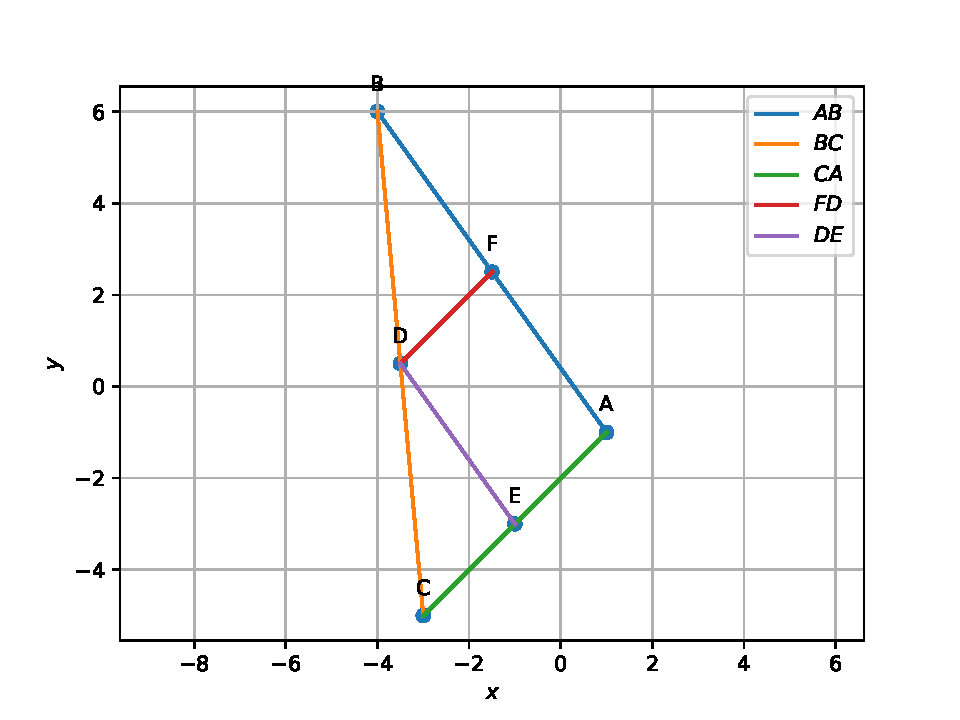
\includegraphics[width=0.75\columnwidth]{figs/triangle/pgm.pdf}
\caption{$AFDE$ forms a parallelogram in triangle ABC}
\label{fig:Triangle-pgm}
\end{figure}






















\item   Points $\vec{A}, \vec{B}, \vec{C}$ are defined to be collinear if 
		\begin{align}
			\label{eq:app-app-line-rank}
			\rank{\myvec{1 & 1 & 1 \\ \vec{A}& \vec{B}&\vec{C}}} = 2
		\end{align}
Are the given points in
			\eqref{eq:app-tri-pts}
collinear?
\\
\solution 
From 
			\eqref{eq:app-tri-pts},
\begin{align}
    \label{eq:app-1.1.3,2}
\myvec{
    1 & 1 & 1\\
    \vec{A} & \vec{B} & \vec{C} \\
    } 
    =
    %\label{eq:app-matthrowoperations}
    \myvec{
    1 & 1 & 1
    \\
    1 & -4 & -3
    \\
    -1 & 6 & -5
    }
     \xleftrightarrow[]{R_3 \leftarrow R_3+R_2}
    \myvec{
    1 & 1 & 1
    \\
    1 & -4 & -3
    \\
    0 & 2 & -8 
    }
    \\
     \xleftrightarrow[]{R_2\leftarrow R_1-R_2}
    \myvec{
    1 & 1 & 1
    \\
    0 & 5 & 4
    \\
    0 & 2 & -8 
    }
     \xleftrightarrow[]{R_3\leftarrow R_3-\frac{2}{5}R_2}
    \myvec{
    1 & 1 & 1
    \\
    0 & 5 & 4
    \\
    0 & 0 & \frac{-48}{5}
    }
\end{align}
There are no zero rows. So,
\begin{align}
    \text{rank}\myvec{
    1 & 1 & 1\\
    \vec{A} & \vec{B} & \vec{C} \\
    } &= 3 
\end{align}  
Hence,  the points $\vec{A},\vec{B},\vec{C}$ are not collinear. 
This is visible in 
\figref{fig1:Triangle}.
\begin{figure}[H]
\centering
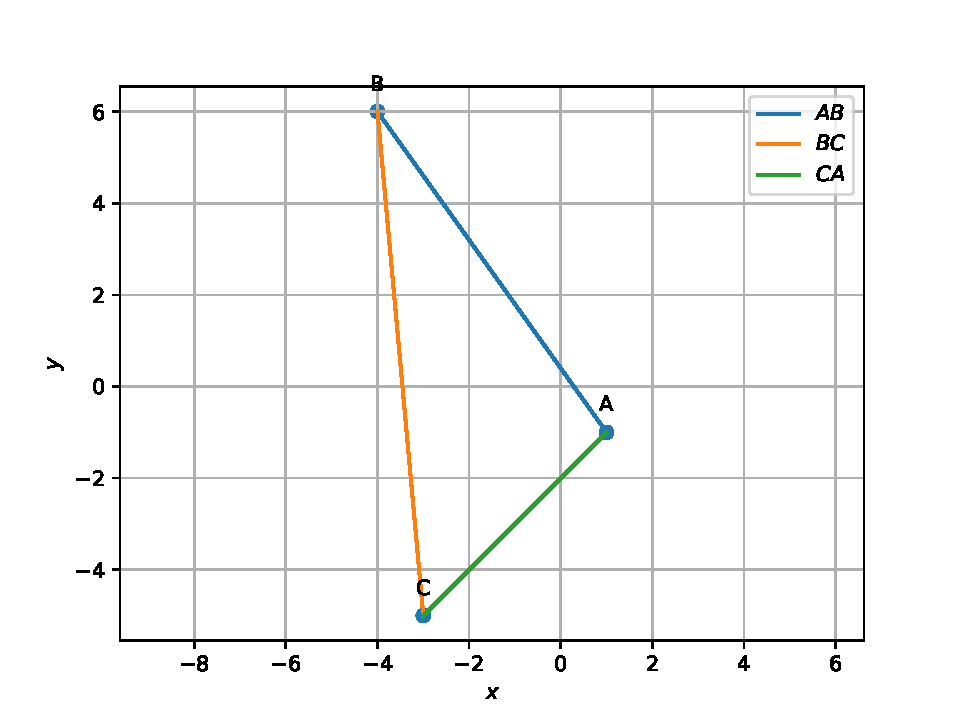
\includegraphics[width=0.75\columnwidth]{figs/triangle/vector.pdf}
\caption{$\triangle ABC$}
\label{fig1:Triangle}
\end{figure}
% \\		\\ \solution 
\begin{align}
    \vec{A}-\vec{F}&=\myvec{1\\-1}-\myvec{\frac{-3}{2}\\\frac{5}{2}}
    =\myvec{\frac{5}{2}\\\frac{-7}{2}}
    \\
    \vec{E}-\vec{D}&=\myvec{-1\\-3}-\myvec{\frac{-7}{2}\\\frac{1}{2}}
    =\myvec{\frac{5}{2}\\\frac{-7}{2}}
    \\
	\implies	\vec{A}-\vec{F} &= \vec{E}-\vec{D}
\end{align}
See \figref{fig:Triangle-pgm}, 
\begin{figure}
\centering
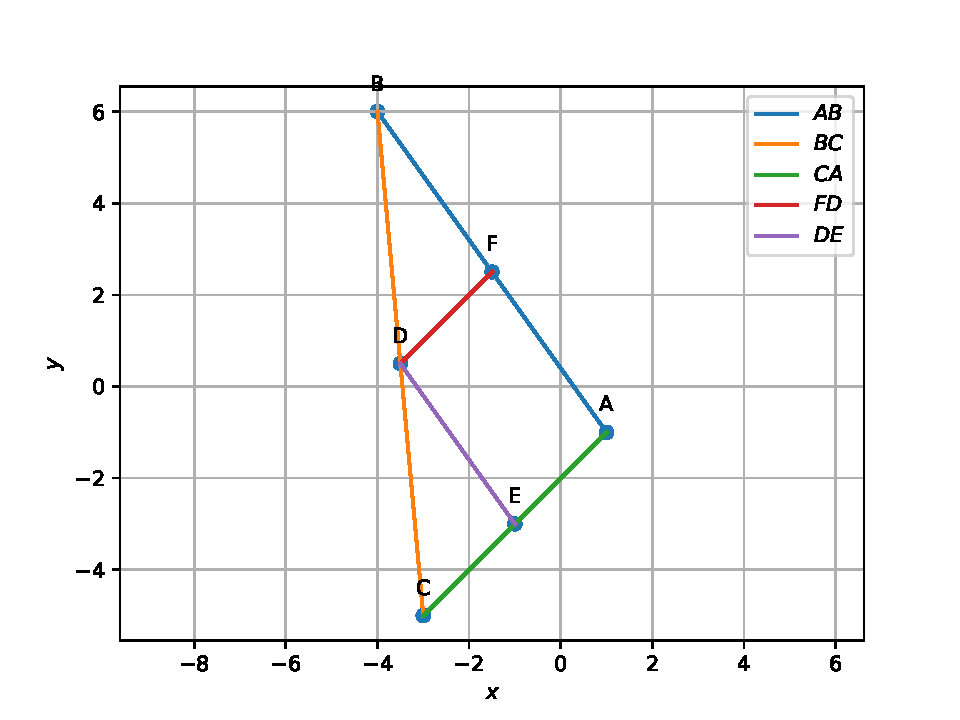
\includegraphics[width=0.75\columnwidth]{figs/triangle/pgm.pdf}
\caption{$AFDE$ forms a parallelogram in triangle ABC}
\label{fig:Triangle-pgm}
\end{figure}






















\item The parameteric form of the equation  of $AB$ is 
		\begin{align}
			\label{eq:app-geo-param}
			\vec{x}=\vec{A}+k\vec{m} \quad k \ne 0,
		\end{align}
		where
		\begin{align}
\vec{m}=\vec{B}-\vec{A}
		\end{align}
is the direction vector of $AB$.
Find the parameteric equations of $AB, BC$ and $CA$.
\\
\solution
From 
			\eqref{eq:app-geo-param} and
		\eqref{eq:app-geo-dir-vec-ab},
the parametric equation for $AB$ is given by
\begin{align}
AB: \vec{x} = &\myvec{1\\-1} + k \myvec{-5\\7}
\end{align}
Similarly, from 
		\eqref{eq:app-geo-dir-vec-bc} and
		\eqref{eq:app-geo-dir-vec-ca},
\begin{align}
BC: \vec{x} = &\myvec{-4\\6} + k \myvec{1\\-11}\\
CA: \vec{x} = &\myvec{-3\\-5} + k \myvec{4\\4}
\end{align}

%		\\ \solution 
\begin{align}
    \vec{A}-\vec{F}&=\myvec{1\\-1}-\myvec{\frac{-3}{2}\\\frac{5}{2}}
    =\myvec{\frac{5}{2}\\\frac{-7}{2}}
    \\
    \vec{E}-\vec{D}&=\myvec{-1\\-3}-\myvec{\frac{-7}{2}\\\frac{1}{2}}
    =\myvec{\frac{5}{2}\\\frac{-7}{2}}
    \\
	\implies	\vec{A}-\vec{F} &= \vec{E}-\vec{D}
\end{align}
See \figref{fig:Triangle-pgm}, 
\begin{figure}
\centering
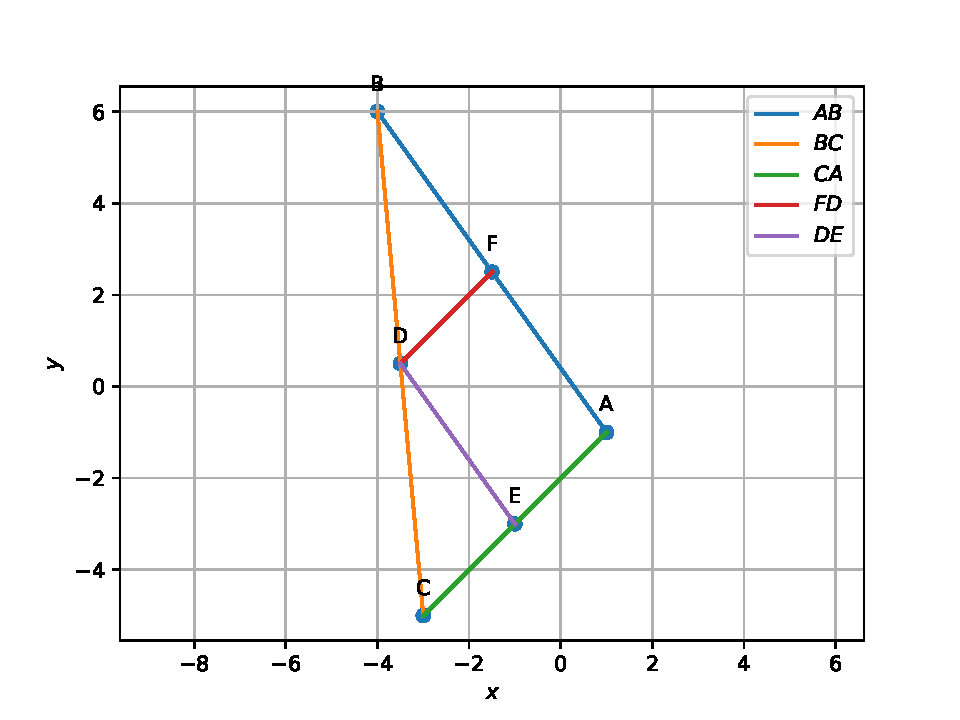
\includegraphics[width=0.75\columnwidth]{figs/triangle/pgm.pdf}
\caption{$AFDE$ forms a parallelogram in triangle ABC}
\label{fig:Triangle-pgm}
\end{figure}






















\item The normal form of the equation of $AB$  is 
		\begin{align}
			\label{eq:app-geo-normal}
			\vec{n}^{\top}\brak{	\vec{x}-\vec{A}} = 0
		\end{align}
		where 
		\begin{align}
			\vec{n}^{\top}\vec{m}&=\vec{n}^{\top}\brak{\vec{B}-\vec{A}} = 0
			\\
			\text{or, } \vec{n}&=\myvec{0 & 1 \\ -1 & 0} \vec{m}
			\label{eq:app-geo-norm-vec}
		\end{align}
Find the normal form of the equations of $AB, BC$ and $CA$.
\\
\solution
\begin{enumerate}
	\item
From
		\eqref{eq:app-geo-dir-vec-bc}, 
the direction vector of side $\vec{BC}$ is
\begin{align}
\vec{m}
	&=\myvec{1\\-11}
	\\
\implies \vec{n} &= \myvec{0 & 1\\
  -1 & 0}\myvec{1\\-11}
 = \myvec{-11\\-1}
		\label{eq:app-geo-norm-vec-bc}
\end{align}
from 
			\eqref{eq:app-geo-norm-vec}.
Hence, from 
			\eqref{eq:app-geo-normal},
the normal equation of side $BC$ is 
\begin{align}
	\vec{n}^{\top}\brak{	\vec{x}-\vec{B}} &= 0
			\\
\implies    \myvec{-11 & -1}\vec{x}&=\myvec{-11 & -1}\myvec{-4\\6}\\
    \implies
BC: \quad    \myvec{11 & 1}\vec{x}&=-38
\end{align}
\item Similarly, for $AB$,
from 
		\eqref{eq:app-geo-dir-vec-ab}, 
\begin{align}
	\vec{m} &= \myvec{-5\\7}
	\\
\implies        \vec{n} 
                &= \myvec{0&1\\-1&0}\myvec{-5\\7}
                = \myvec{7\\5}
		\label{eq:app-geo-norm-vec-ab}
\end{align}
and 
\begin{align}
	\vec{n}^{\top}\brak{	\vec{x}-\vec{A}} &= 0
	\\
	\implies
                AB: \quad  \vec{n}^{\top}\vec{x} &= \myvec{7&5}\myvec{1\\-1}\\    
       \implies\myvec{7&5}\vec{x} &= 2
\end{align}
\item For 
$CA$, 
from 
		\eqref{eq:app-geo-dir-vec-ca}, 
\begin{align}
\vec{m} &= \myvec{1 \\ 1}
\\
		\label{eq:app-geo-norm-vec-ca}
\implies \vec{n} 
&= \myvec{0&1 \\ -1&0}\myvec{1 \\ 1}
= \myvec{1 \\ -1}\\
\\
\implies	\vec{n}^{\top}\brak{	\vec{x}-\vec{C}} &= 0
\\
\implies \myvec{1&-1}{\vec{x}} &= \myvec{1&-1}\myvec{-3 \\ -5} 
= 2 
\end{align}
\end{enumerate}

%\begin{enumerate}
	\item
From
		\eqref{eq:geo-dir-vec-bc}, 
the direction vector of side $\vec{BC}$ is
\begin{align}
\vec{m}
	&=\myvec{1\\-11}
	\\
\implies \vec{n} &= \myvec{0 & 1\\
  -1 & 0}\myvec{1\\-11}
 = \myvec{-11\\-1}
		\label{eq:geo-norm-vec-bc}
\end{align}
from 
			\eqref{eq:geo-norm-vec}.
Hence, from 
			\eqref{eq:geo-normal},
the normal equation of side $BC$ is 
\begin{align}
	\vec{n}^{\top}\brak{	\vec{x}-\vec{B}} &= 0
			\\
\implies    \myvec{-11 & -1}\vec{x}&=\myvec{-11 & -1}\myvec{-4\\6}\\
    \implies
BC: \quad    \myvec{11 & 1}\vec{x}&=-38
\end{align}
\item Similarly, for $AB$,
from 
		\eqref{eq:geo-dir-vec-ab}, 
\begin{align}
	\vec{m} &= \myvec{-5\\7}
	\\
\implies        \vec{n} 
                &= \myvec{0&1\\-1&0}\myvec{-5\\7}
                = \myvec{7\\5}
		\label{eq:geo-norm-vec-ab}
\end{align}
and 
\begin{align}
	\vec{n}^{\top}\brak{	\vec{x}-\vec{A}} &= 0
	\\
	\implies
                AB: \quad  \vec{n}^{\top}\vec{x} &= \myvec{7&5}\myvec{1\\-1}\\    
       \implies\myvec{7&5}\vec{x} &= 2
\end{align}
\item For 
$CA$, 
from 
		\eqref{eq:geo-dir-vec-ca}, 
\begin{align}
\vec{m} &= \myvec{1 \\ 1}
\\
		\label{eq:geo-norm-vec-ca}
\implies \vec{n} 
&= \myvec{0&1 \\ -1&0}\myvec{1 \\ 1}
= \myvec{1 \\ -1}\\
\\
\implies	\vec{n}^{\top}\brak{	\vec{x}-\vec{C}} &= 0
\\
\implies \myvec{1&-1}{\vec{x}} &= \myvec{1&-1}\myvec{-3 \\ -5} 
= 2 
\end{align}
\end{enumerate}


\item The area of $\triangle ABC$ is defined as
		\begin{align}
			\label{eq:app-tri-area-cross}
			\frac{1}{2}\norm{{\brak{\vec{A}-\vec{B}}\times \brak{\vec{A}-\vec{C}}}}
		\end{align}
		where
		\begin{align}
			\vec{A}\times\vec{B} \triangleq \mydet{1 & -4 \\-1 & 6}
		\end{align}
		Find the area of $\triangle ABC$.\\
\solution
From
		\eqref{eq:app-geo-dir-vec-ab}
		and
		\eqref{eq:app-geo-dir-vec-ca},
\begin{align}
	\vec{A}-\vec{B}=\myvec{5\\-7},
	\vec{A}-\vec{C}&=\myvec{4\\4}\\
\implies (\vec{A}-\vec{B})\times(\vec{A}-\vec{C}) &=\mydet{5 & 4\\-7 & 4}\\
&=5\times 4-4\times (-7)\\&=48\\
\implies\frac{1}{2}\norm{(\vec{A}-\vec{B})\times(\vec{A}-\vec{C})}&=\frac{48}{2}=24
\end{align}
which is the desired area.

%  		\\ \solution 
\begin{align}
    \vec{A}-\vec{F}&=\myvec{1\\-1}-\myvec{\frac{-3}{2}\\\frac{5}{2}}
    =\myvec{\frac{5}{2}\\\frac{-7}{2}}
    \\
    \vec{E}-\vec{D}&=\myvec{-1\\-3}-\myvec{\frac{-7}{2}\\\frac{1}{2}}
    =\myvec{\frac{5}{2}\\\frac{-7}{2}}
    \\
	\implies	\vec{A}-\vec{F} &= \vec{E}-\vec{D}
\end{align}
See \figref{fig:Triangle-pgm}, 
\begin{figure}
\centering
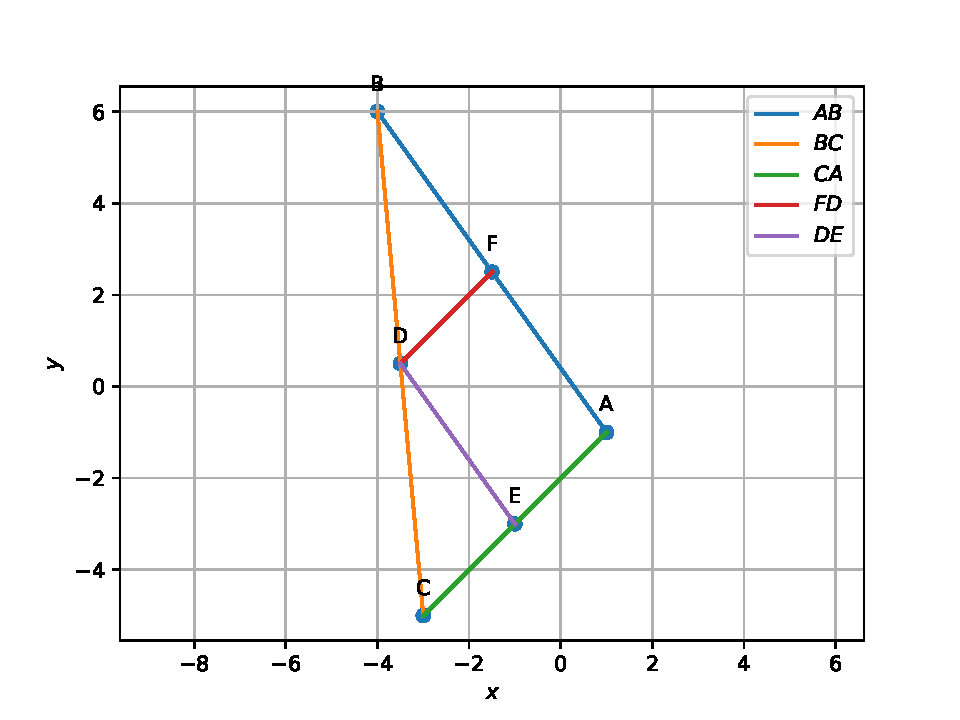
\includegraphics[width=0.75\columnwidth]{figs/triangle/pgm.pdf}
\caption{$AFDE$ forms a parallelogram in triangle ABC}
\label{fig:Triangle-pgm}
\end{figure}






















	\item Find the angles $A, B, C$ if 
%    \label{prop:angle2d}
  \begin{align}
    \label{eq:app-angle2d}
			\cos A \triangleq 
\frac{\brak{\vec{B}-\vec{A}}^{\top}{\vec{C}-\vec{A}}}{\norm{\vec{B}-\vec{A}}\norm{\vec{C}-\vec{A}}}
  \end{align}\\
  \solution
\begin{enumerate}
	\item From 
		\eqref{eq:app-geo-dir-vec-ab},
		\eqref{eq:app-geo-dir-vec-ca},
		\eqref{eq:app-geo-norm-ab}
		and
		\eqref{eq:app-geo-norm-ca}
\begin{align}
	(\vec{B}-\vec{A})^{\top}(\vec{C}-\vec{A})&=\myvec{-5&7}\myvec{-4\\-4}\\
	&=-8
	\\
	\implies
	\cos{A}&= \frac{-8}{\sqrt{74} \sqrt{32}}
	= \frac{-1}{\sqrt{37}}\\
	\implies A&=\cos^{-1}{\frac{-1}{\sqrt{37}}}
\end{align}
	\item From 
		\eqref{eq:app-geo-dir-vec-ab},
		\eqref{eq:app-geo-dir-vec-bc},
		\eqref{eq:app-geo-norm-ab}
		and
		\eqref{eq:app-geo-norm-bc}
\begin{align}
	(\vec{C}-\vec{B})^{\top}(\vec{A}-\vec{B})&=\myvec{1&-11}\myvec{5\\-7}\\
	&= 82
	\\
	\implies
	\cos{B}&= \frac{82}{\sqrt{74} \sqrt{122}}
	= \frac{41}{\sqrt{2257}}\\
	\implies B&=\cos^{-1}{\frac{41}{\sqrt{2257}}}
\end{align}
	\item From 
		\eqref{eq:app-geo-dir-vec-bc},
		\eqref{eq:app-geo-dir-vec-ca},
		\eqref{eq:app-geo-norm-bc}
		and
		\eqref{eq:app-geo-norm-ca}
\begin{align}
	(\vec{A}-\vec{C})^{\top}(\vec{B}-\vec{C})&=\myvec{4&4}\myvec{-1\\11}\\
	&=40
	\\
\implies	\cos{C}&= \frac{40}{\sqrt{32} \sqrt{122}}
	= \frac{5}{\sqrt{61}}\\
	\implies C&=\cos^{-1}{\frac{5}{\sqrt{61}}}
\end{align}

\end{enumerate}
%  	\\ \solution 
\begin{align}
    \vec{A}-\vec{F}&=\myvec{1\\-1}-\myvec{\frac{-3}{2}\\\frac{5}{2}}
    =\myvec{\frac{5}{2}\\\frac{-7}{2}}
    \\
    \vec{E}-\vec{D}&=\myvec{-1\\-3}-\myvec{\frac{-7}{2}\\\frac{1}{2}}
    =\myvec{\frac{5}{2}\\\frac{-7}{2}}
    \\
	\implies	\vec{A}-\vec{F} &= \vec{E}-\vec{D}
\end{align}
See \figref{fig:Triangle-pgm}, 
\begin{figure}
\centering
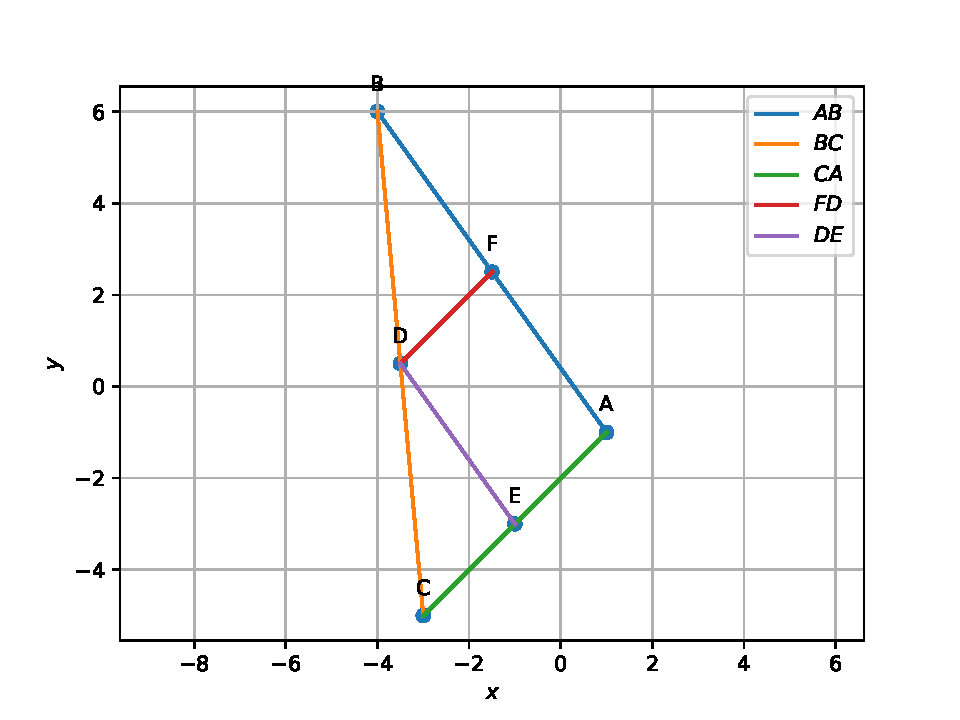
\includegraphics[width=0.75\columnwidth]{figs/triangle/pgm.pdf}
\caption{$AFDE$ forms a parallelogram in triangle ABC}
\label{fig:Triangle-pgm}
\end{figure}






















All codes for this section are available at
\begin{lstlisting}
	codes/triangle/sides.py
\end{lstlisting}
\end{enumerate}

\item Find the values of $x, y, z$ so that the vectors 
$x\hat{i}+2\hat{j}+z\hat{k}$
and 
$2\hat{i}+y\hat{j}+\hat{k}$
are equal.
\item Find the sum of the vectors $\vec{a}=\hat{i}-2\hat{j}+\hat{k}$,  $\vec{b}=-2\hat{i}+4\hat{j}+5\hat{k}$ and $\vec{c}=\hat{i}-6\hat{j}-7\hat{k}$.
\item Find the slope of a line,  which passes through the origin and the mid point of the line segment joining the points $\vec{P}$(0, -4) and $\vec{B}$(8, 0).
\label{chapters/11/10/1/5}
	\\
	\solution
The direction vector
\begin{align}
	\vec{B}-\vec{A}
	=
	\myvec{
  h-x_1\\
  k-y_1
  }
   \equiv
	\myvec{
1\\
	\frac{ k-y_1}{h-x_1}
  }
  \\
	\implies m = 
	\frac{ k-y_1}{h-x_1},
\end{align}
yielding the desired result.

\item Find the angle between x-axis and the line joining points (3, -1) and (4, -2).
\label{chapters/11/10/1/10}
\\
\solution 
The direction vector
\begin{align}
	\vec{B}-\vec{A}
	=
	\myvec{
  h-x_1\\
  k-y_1
  }
   \equiv
	\myvec{
1\\
	\frac{ k-y_1}{h-x_1}
  }
  \\
	\implies m = 
	\frac{ k-y_1}{h-x_1},
\end{align}
yielding the desired result.

\item A line passes through $\vec{A}(x_1, y_1)$ and $\vec{B}(h, k)$. If slope of the line is m,  show that $(k-y_1)=m(h-x_1)$.
\label{chapters/11/10/1/12}
\\
\solution 
The direction vector
\begin{align}
	\vec{B}-\vec{A}
	=
	\myvec{
  h-x_1\\
  k-y_1
  }
   \equiv
	\myvec{
1\\
	\frac{ k-y_1}{h-x_1}
  }
  \\
	\implies m = 
	\frac{ k-y_1}{h-x_1},
\end{align}
yielding the desired result.

\item
Show that the line through the points \brak{4, 7, 8}, \brak{2, 3, 4} is parallel to the line through the points \brak{-1, -2, 1}, \brak{1, 2, 5}.
	\label{12.11.2.3}
\\
\solution
	\begin{align}
\myvec{4 \\ 7 \\ 8}- \myvec{2 \\ 3 \\ 4}= \myvec{-1 \\ -2 \\ 1}- \myvec{1 \\ 2 \\ 5}
\equiv \myvec{2\\4\\4}
\end{align}
which means that the given lines have the same direction vector and are hence parallel.

\item The vector having intial and terminal points as (-2, 5, 0) and (3, 7, 4), respectively is
\solution
The desired vector is
\begin{align}
	\myvec{3 \\ 7 \\ 4}
	-\myvec{-2 \\ 5 \\ 0} = 
	\myvec{5 \\ 2 \\ 4}  
\end{align}
\item Find the vector joining the points $\vec{P}\brak{2, 3, 0}$ and $\vec{Q}\brak{-1, -2, -4}$ directed from $\vec{P}$ to $\vec{Q}$.
\item Without using distance formula,  show that points $\vec{A}(– 2,  – 1),  \vec{B}(4,  0),  \vec{C}(3,  3)$ and $\vec{D}(–3,  2)$ are the vertices of a parallelogram.
\label{chapters/11/10/1/9}
\\
\solution
%\renewcommand{\theequation}{\theenumi}
\begin{enumerate}[label=\thesubsection.\arabic*.,ref=\thesubsection.\theenumi]
%\numberwithin{equation}{enumi}
\item The direction vector of $AB$ is defined as
		\begin{align}
			\vec{B}-
			\vec{A}
		\end{align}
Find the direction vectors of $AB, BC$ and $CA$.
\\
\solution 
\begin{enumerate} 
\item  The Direction vector of $AB$ is 
	\begin{align}  \vec{B} - \vec{A} 
		=\myvec{ -4\\ 6 } - \myvec{ 1\\ -1 }
 = \myvec{ -4 - 1\\ 6 - (-1) } = \myvec{ -5\\ 7 }
		\label{eq:app-geo-dir-vec-ab}
 \end{align}
\item The Direction vector of $BC$ is
	\begin{align} \vec{C} - \vec{B}=\myvec{ -3\\ -5} - \myvec{ -4\\ 6 }
 = \myvec{ -3 - (-4)\\ -5 - 6 } = \myvec{1\\ -11 }
		\label{eq:app-geo-dir-vec-bc}
  \end{align}
  \item  The Direction vector of $CA$  is
	  \begin{align}  \vec{A} - \vec{C} =\myvec{ 1\\ -1 }-\myvec{ -3\\ -5}
 = \myvec{ 1 - (-3)\\ -1 - (-5) } = \myvec{ 4\\ 4 }
		\label{eq:app-geo-dir-vec-ca}
  \end{align}
 \end{enumerate}
%	\solution 
\begin{enumerate} 
\item  The Direction vector of $AB$ is 
	\begin{align}  \vec{B} - \vec{A} 
		=\myvec{ -4\\ 6 } - \myvec{ 1\\ -1 }
 = \myvec{ -4 - 1\\ 6 - (-1) } = \myvec{ -5\\ 7 }
		\label{eq:geo-dir-vec-ab}
 \end{align}
\item The Direction vector of $BC$ is
	\begin{align} \vec{C} - \vec{B}=\myvec{ -3\\ -5} - \myvec{ -4\\ 6 }
 = \myvec{ -3 - (-4)\\ -5 - 6 } = \myvec{1\\ -11 }
		\label{eq:geo-dir-vec-bc}
  \end{align}
  \item  The Direction vector of $CA$  is
	  \begin{align}  \vec{A} - \vec{C} =\myvec{ 1\\ -1 }-\myvec{ -3\\ -5}
 = \myvec{ 1 - (-3)\\ -1 - (-5) } = \myvec{ 4\\ 4 }
		\label{eq:geo-dir-vec-ca}
  \end{align}
 \end{enumerate}


	\item The length of side $BC$ is 
		\label{prob:side-length}
		\begin{align}
			c = \norm{\vec{B}-\vec{A}} \triangleq \sqrt{\brak{\vec{B}-\vec{A}}^{\top}\brak{\vec{B}-\vec{A}}}
		\end{align}
		where
		\begin{align}
			\vec{A}^{\top}\triangleq\myvec{1 & -1}
		\end{align}
		Similarly, 
		\begin{align}
b = \norm{\vec{C}-\vec{B}},\,
a = \norm{\vec{A}-\vec{C}}
		\end{align}
		Find $a, b, c$.
\begin{enumerate}
	\item 
	From 	
		\eqref{eq:app-geo-dir-vec-ab},
\begin{align}
\vec{A}-\vec{B} &= \myvec{5\\-7}, \\
\implies 	c &= 	\norm{\vec{B}-\vec{A}} = \norm{\vec{A}-\vec{B}} 
	\\
	&= \sqrt{\myvec{5 & -7}\myvec{5\\-7}}
= \sqrt{\brak{5}^2 +\brak{7}^2}\\
	&=\sqrt{74}
		\label{eq:app-geo-norm-ab}
\end{align}
	\item Similarly, from 
		\eqref{eq:app-geo-dir-vec-bc},
\begin{align}
	a &= \norm{\vec{B}-\vec{C}} 
	= \sqrt{\myvec{-1 & 11}\myvec{-1\\11}}
\\
&= \sqrt{\brak{1}^2+\brak{11}^2}
	= \sqrt{122}
		\label{eq:app-geo-norm-bc}
\end{align}
and
		from 		\eqref{eq:app-geo-dir-vec-ca},
	\item 
		\begin{align}
			b &= \norm{\vec{A}-\vec{C}} = \sqrt{\myvec{4 & 4}\myvec{4\\4}}
\\
&= \sqrt{\brak{4}^2+\brak{4}^2}
	=\sqrt{32}
		\label{eq:app-geo-norm-ca}
\end{align}
\end{enumerate}
%  \\            
  %\\ \solution 
\begin{align}
    \vec{A}-\vec{F}&=\myvec{1\\-1}-\myvec{\frac{-3}{2}\\\frac{5}{2}}
    =\myvec{\frac{5}{2}\\\frac{-7}{2}}
    \\
    \vec{E}-\vec{D}&=\myvec{-1\\-3}-\myvec{\frac{-7}{2}\\\frac{1}{2}}
    =\myvec{\frac{5}{2}\\\frac{-7}{2}}
    \\
	\implies	\vec{A}-\vec{F} &= \vec{E}-\vec{D}
\end{align}
See \figref{fig:Triangle-pgm}, 
\begin{figure}
\centering
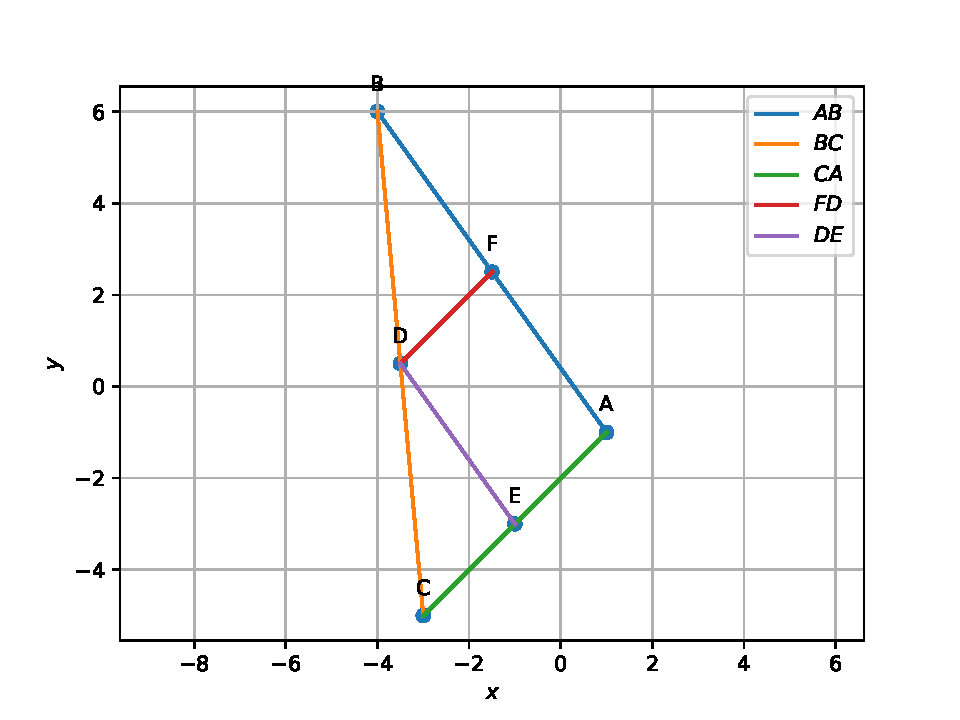
\includegraphics[width=0.75\columnwidth]{figs/triangle/pgm.pdf}
\caption{$AFDE$ forms a parallelogram in triangle ABC}
\label{fig:Triangle-pgm}
\end{figure}






















\item   Points $\vec{A}, \vec{B}, \vec{C}$ are defined to be collinear if 
		\begin{align}
			\label{eq:app-app-line-rank}
			\rank{\myvec{1 & 1 & 1 \\ \vec{A}& \vec{B}&\vec{C}}} = 2
		\end{align}
Are the given points in
			\eqref{eq:app-tri-pts}
collinear?
\\
\solution 
From 
			\eqref{eq:app-tri-pts},
\begin{align}
    \label{eq:app-1.1.3,2}
\myvec{
    1 & 1 & 1\\
    \vec{A} & \vec{B} & \vec{C} \\
    } 
    =
    %\label{eq:app-matthrowoperations}
    \myvec{
    1 & 1 & 1
    \\
    1 & -4 & -3
    \\
    -1 & 6 & -5
    }
     \xleftrightarrow[]{R_3 \leftarrow R_3+R_2}
    \myvec{
    1 & 1 & 1
    \\
    1 & -4 & -3
    \\
    0 & 2 & -8 
    }
    \\
     \xleftrightarrow[]{R_2\leftarrow R_1-R_2}
    \myvec{
    1 & 1 & 1
    \\
    0 & 5 & 4
    \\
    0 & 2 & -8 
    }
     \xleftrightarrow[]{R_3\leftarrow R_3-\frac{2}{5}R_2}
    \myvec{
    1 & 1 & 1
    \\
    0 & 5 & 4
    \\
    0 & 0 & \frac{-48}{5}
    }
\end{align}
There are no zero rows. So,
\begin{align}
    \text{rank}\myvec{
    1 & 1 & 1\\
    \vec{A} & \vec{B} & \vec{C} \\
    } &= 3 
\end{align}  
Hence,  the points $\vec{A},\vec{B},\vec{C}$ are not collinear. 
This is visible in 
\figref{fig1:Triangle}.
\begin{figure}[H]
\centering
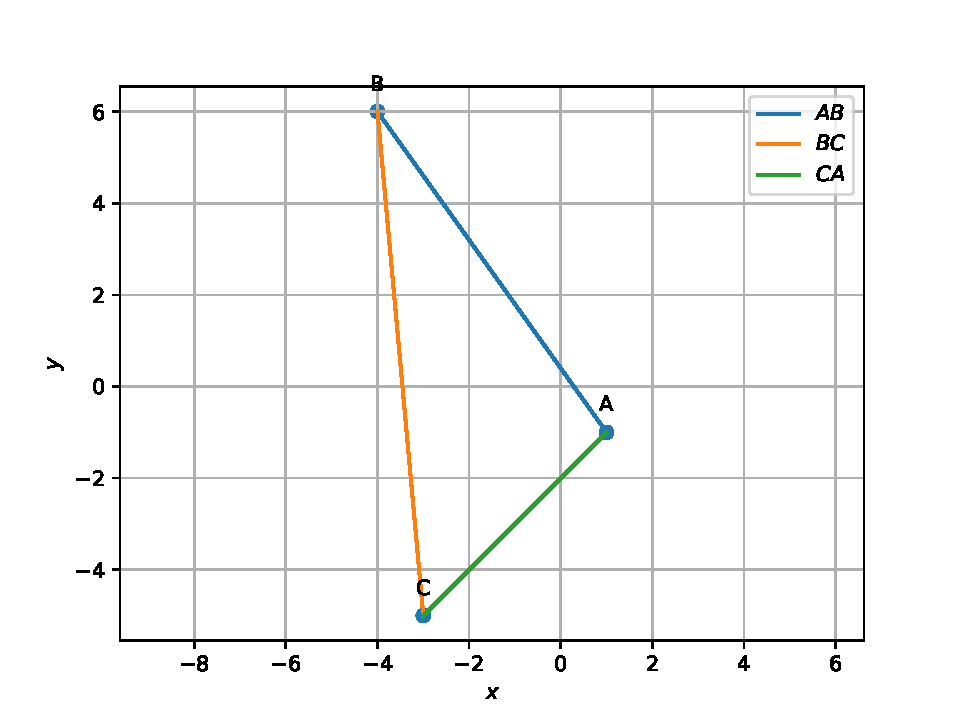
\includegraphics[width=0.75\columnwidth]{figs/triangle/vector.pdf}
\caption{$\triangle ABC$}
\label{fig1:Triangle}
\end{figure}
% \\		\\ \solution 
\begin{align}
    \vec{A}-\vec{F}&=\myvec{1\\-1}-\myvec{\frac{-3}{2}\\\frac{5}{2}}
    =\myvec{\frac{5}{2}\\\frac{-7}{2}}
    \\
    \vec{E}-\vec{D}&=\myvec{-1\\-3}-\myvec{\frac{-7}{2}\\\frac{1}{2}}
    =\myvec{\frac{5}{2}\\\frac{-7}{2}}
    \\
	\implies	\vec{A}-\vec{F} &= \vec{E}-\vec{D}
\end{align}
See \figref{fig:Triangle-pgm}, 
\begin{figure}
\centering
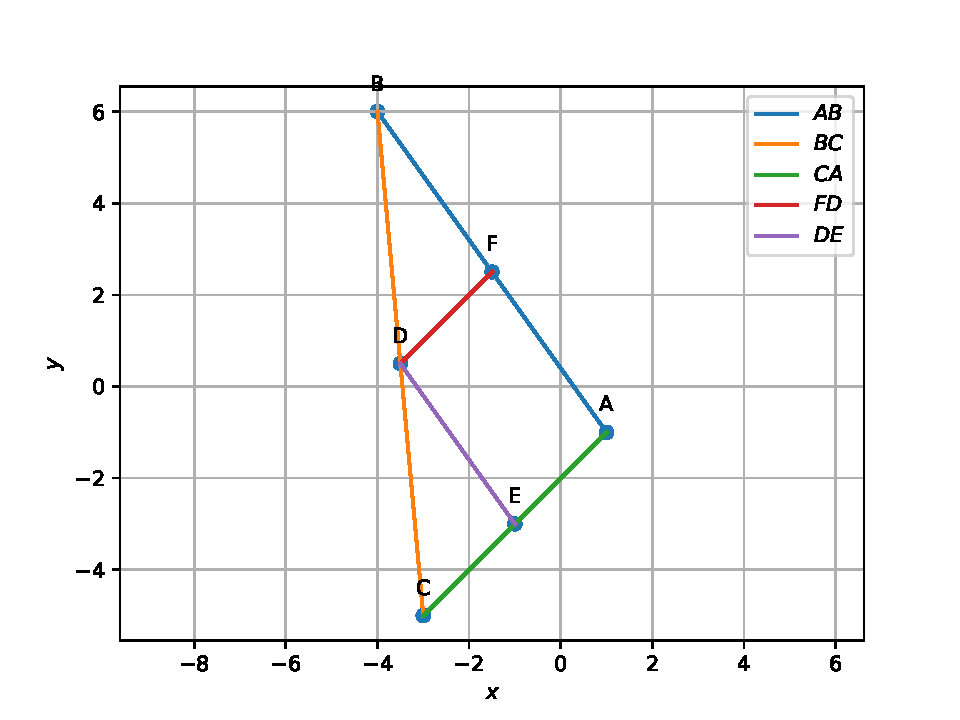
\includegraphics[width=0.75\columnwidth]{figs/triangle/pgm.pdf}
\caption{$AFDE$ forms a parallelogram in triangle ABC}
\label{fig:Triangle-pgm}
\end{figure}






















\item The parameteric form of the equation  of $AB$ is 
		\begin{align}
			\label{eq:app-geo-param}
			\vec{x}=\vec{A}+k\vec{m} \quad k \ne 0,
		\end{align}
		where
		\begin{align}
\vec{m}=\vec{B}-\vec{A}
		\end{align}
is the direction vector of $AB$.
Find the parameteric equations of $AB, BC$ and $CA$.
\\
\solution
From 
			\eqref{eq:app-geo-param} and
		\eqref{eq:app-geo-dir-vec-ab},
the parametric equation for $AB$ is given by
\begin{align}
AB: \vec{x} = &\myvec{1\\-1} + k \myvec{-5\\7}
\end{align}
Similarly, from 
		\eqref{eq:app-geo-dir-vec-bc} and
		\eqref{eq:app-geo-dir-vec-ca},
\begin{align}
BC: \vec{x} = &\myvec{-4\\6} + k \myvec{1\\-11}\\
CA: \vec{x} = &\myvec{-3\\-5} + k \myvec{4\\4}
\end{align}

%		\\ \solution 
\begin{align}
    \vec{A}-\vec{F}&=\myvec{1\\-1}-\myvec{\frac{-3}{2}\\\frac{5}{2}}
    =\myvec{\frac{5}{2}\\\frac{-7}{2}}
    \\
    \vec{E}-\vec{D}&=\myvec{-1\\-3}-\myvec{\frac{-7}{2}\\\frac{1}{2}}
    =\myvec{\frac{5}{2}\\\frac{-7}{2}}
    \\
	\implies	\vec{A}-\vec{F} &= \vec{E}-\vec{D}
\end{align}
See \figref{fig:Triangle-pgm}, 
\begin{figure}
\centering
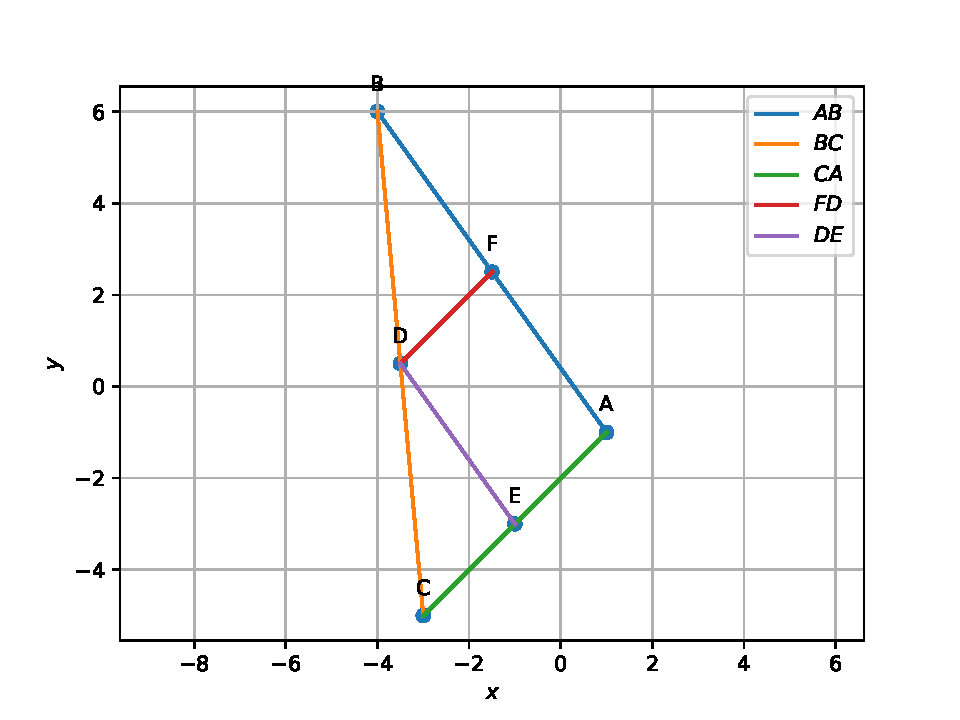
\includegraphics[width=0.75\columnwidth]{figs/triangle/pgm.pdf}
\caption{$AFDE$ forms a parallelogram in triangle ABC}
\label{fig:Triangle-pgm}
\end{figure}






















\item The normal form of the equation of $AB$  is 
		\begin{align}
			\label{eq:app-geo-normal}
			\vec{n}^{\top}\brak{	\vec{x}-\vec{A}} = 0
		\end{align}
		where 
		\begin{align}
			\vec{n}^{\top}\vec{m}&=\vec{n}^{\top}\brak{\vec{B}-\vec{A}} = 0
			\\
			\text{or, } \vec{n}&=\myvec{0 & 1 \\ -1 & 0} \vec{m}
			\label{eq:app-geo-norm-vec}
		\end{align}
Find the normal form of the equations of $AB, BC$ and $CA$.
\\
\solution
\begin{enumerate}
	\item
From
		\eqref{eq:app-geo-dir-vec-bc}, 
the direction vector of side $\vec{BC}$ is
\begin{align}
\vec{m}
	&=\myvec{1\\-11}
	\\
\implies \vec{n} &= \myvec{0 & 1\\
  -1 & 0}\myvec{1\\-11}
 = \myvec{-11\\-1}
		\label{eq:app-geo-norm-vec-bc}
\end{align}
from 
			\eqref{eq:app-geo-norm-vec}.
Hence, from 
			\eqref{eq:app-geo-normal},
the normal equation of side $BC$ is 
\begin{align}
	\vec{n}^{\top}\brak{	\vec{x}-\vec{B}} &= 0
			\\
\implies    \myvec{-11 & -1}\vec{x}&=\myvec{-11 & -1}\myvec{-4\\6}\\
    \implies
BC: \quad    \myvec{11 & 1}\vec{x}&=-38
\end{align}
\item Similarly, for $AB$,
from 
		\eqref{eq:app-geo-dir-vec-ab}, 
\begin{align}
	\vec{m} &= \myvec{-5\\7}
	\\
\implies        \vec{n} 
                &= \myvec{0&1\\-1&0}\myvec{-5\\7}
                = \myvec{7\\5}
		\label{eq:app-geo-norm-vec-ab}
\end{align}
and 
\begin{align}
	\vec{n}^{\top}\brak{	\vec{x}-\vec{A}} &= 0
	\\
	\implies
                AB: \quad  \vec{n}^{\top}\vec{x} &= \myvec{7&5}\myvec{1\\-1}\\    
       \implies\myvec{7&5}\vec{x} &= 2
\end{align}
\item For 
$CA$, 
from 
		\eqref{eq:app-geo-dir-vec-ca}, 
\begin{align}
\vec{m} &= \myvec{1 \\ 1}
\\
		\label{eq:app-geo-norm-vec-ca}
\implies \vec{n} 
&= \myvec{0&1 \\ -1&0}\myvec{1 \\ 1}
= \myvec{1 \\ -1}\\
\\
\implies	\vec{n}^{\top}\brak{	\vec{x}-\vec{C}} &= 0
\\
\implies \myvec{1&-1}{\vec{x}} &= \myvec{1&-1}\myvec{-3 \\ -5} 
= 2 
\end{align}
\end{enumerate}

%\begin{enumerate}
	\item
From
		\eqref{eq:geo-dir-vec-bc}, 
the direction vector of side $\vec{BC}$ is
\begin{align}
\vec{m}
	&=\myvec{1\\-11}
	\\
\implies \vec{n} &= \myvec{0 & 1\\
  -1 & 0}\myvec{1\\-11}
 = \myvec{-11\\-1}
		\label{eq:geo-norm-vec-bc}
\end{align}
from 
			\eqref{eq:geo-norm-vec}.
Hence, from 
			\eqref{eq:geo-normal},
the normal equation of side $BC$ is 
\begin{align}
	\vec{n}^{\top}\brak{	\vec{x}-\vec{B}} &= 0
			\\
\implies    \myvec{-11 & -1}\vec{x}&=\myvec{-11 & -1}\myvec{-4\\6}\\
    \implies
BC: \quad    \myvec{11 & 1}\vec{x}&=-38
\end{align}
\item Similarly, for $AB$,
from 
		\eqref{eq:geo-dir-vec-ab}, 
\begin{align}
	\vec{m} &= \myvec{-5\\7}
	\\
\implies        \vec{n} 
                &= \myvec{0&1\\-1&0}\myvec{-5\\7}
                = \myvec{7\\5}
		\label{eq:geo-norm-vec-ab}
\end{align}
and 
\begin{align}
	\vec{n}^{\top}\brak{	\vec{x}-\vec{A}} &= 0
	\\
	\implies
                AB: \quad  \vec{n}^{\top}\vec{x} &= \myvec{7&5}\myvec{1\\-1}\\    
       \implies\myvec{7&5}\vec{x} &= 2
\end{align}
\item For 
$CA$, 
from 
		\eqref{eq:geo-dir-vec-ca}, 
\begin{align}
\vec{m} &= \myvec{1 \\ 1}
\\
		\label{eq:geo-norm-vec-ca}
\implies \vec{n} 
&= \myvec{0&1 \\ -1&0}\myvec{1 \\ 1}
= \myvec{1 \\ -1}\\
\\
\implies	\vec{n}^{\top}\brak{	\vec{x}-\vec{C}} &= 0
\\
\implies \myvec{1&-1}{\vec{x}} &= \myvec{1&-1}\myvec{-3 \\ -5} 
= 2 
\end{align}
\end{enumerate}


\item The area of $\triangle ABC$ is defined as
		\begin{align}
			\label{eq:app-tri-area-cross}
			\frac{1}{2}\norm{{\brak{\vec{A}-\vec{B}}\times \brak{\vec{A}-\vec{C}}}}
		\end{align}
		where
		\begin{align}
			\vec{A}\times\vec{B} \triangleq \mydet{1 & -4 \\-1 & 6}
		\end{align}
		Find the area of $\triangle ABC$.\\
\solution
From
		\eqref{eq:app-geo-dir-vec-ab}
		and
		\eqref{eq:app-geo-dir-vec-ca},
\begin{align}
	\vec{A}-\vec{B}=\myvec{5\\-7},
	\vec{A}-\vec{C}&=\myvec{4\\4}\\
\implies (\vec{A}-\vec{B})\times(\vec{A}-\vec{C}) &=\mydet{5 & 4\\-7 & 4}\\
&=5\times 4-4\times (-7)\\&=48\\
\implies\frac{1}{2}\norm{(\vec{A}-\vec{B})\times(\vec{A}-\vec{C})}&=\frac{48}{2}=24
\end{align}
which is the desired area.

%  		\\ \solution 
\begin{align}
    \vec{A}-\vec{F}&=\myvec{1\\-1}-\myvec{\frac{-3}{2}\\\frac{5}{2}}
    =\myvec{\frac{5}{2}\\\frac{-7}{2}}
    \\
    \vec{E}-\vec{D}&=\myvec{-1\\-3}-\myvec{\frac{-7}{2}\\\frac{1}{2}}
    =\myvec{\frac{5}{2}\\\frac{-7}{2}}
    \\
	\implies	\vec{A}-\vec{F} &= \vec{E}-\vec{D}
\end{align}
See \figref{fig:Triangle-pgm}, 
\begin{figure}
\centering
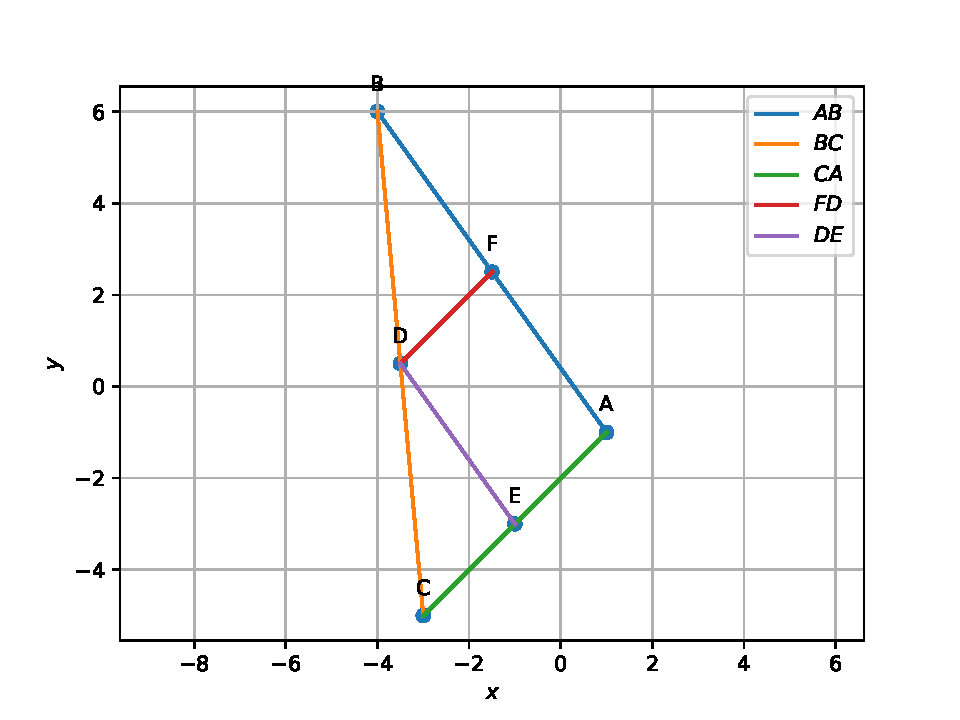
\includegraphics[width=0.75\columnwidth]{figs/triangle/pgm.pdf}
\caption{$AFDE$ forms a parallelogram in triangle ABC}
\label{fig:Triangle-pgm}
\end{figure}






















	\item Find the angles $A, B, C$ if 
%    \label{prop:angle2d}
  \begin{align}
    \label{eq:app-angle2d}
			\cos A \triangleq 
\frac{\brak{\vec{B}-\vec{A}}^{\top}{\vec{C}-\vec{A}}}{\norm{\vec{B}-\vec{A}}\norm{\vec{C}-\vec{A}}}
  \end{align}\\
  \solution
\begin{enumerate}
	\item From 
		\eqref{eq:app-geo-dir-vec-ab},
		\eqref{eq:app-geo-dir-vec-ca},
		\eqref{eq:app-geo-norm-ab}
		and
		\eqref{eq:app-geo-norm-ca}
\begin{align}
	(\vec{B}-\vec{A})^{\top}(\vec{C}-\vec{A})&=\myvec{-5&7}\myvec{-4\\-4}\\
	&=-8
	\\
	\implies
	\cos{A}&= \frac{-8}{\sqrt{74} \sqrt{32}}
	= \frac{-1}{\sqrt{37}}\\
	\implies A&=\cos^{-1}{\frac{-1}{\sqrt{37}}}
\end{align}
	\item From 
		\eqref{eq:app-geo-dir-vec-ab},
		\eqref{eq:app-geo-dir-vec-bc},
		\eqref{eq:app-geo-norm-ab}
		and
		\eqref{eq:app-geo-norm-bc}
\begin{align}
	(\vec{C}-\vec{B})^{\top}(\vec{A}-\vec{B})&=\myvec{1&-11}\myvec{5\\-7}\\
	&= 82
	\\
	\implies
	\cos{B}&= \frac{82}{\sqrt{74} \sqrt{122}}
	= \frac{41}{\sqrt{2257}}\\
	\implies B&=\cos^{-1}{\frac{41}{\sqrt{2257}}}
\end{align}
	\item From 
		\eqref{eq:app-geo-dir-vec-bc},
		\eqref{eq:app-geo-dir-vec-ca},
		\eqref{eq:app-geo-norm-bc}
		and
		\eqref{eq:app-geo-norm-ca}
\begin{align}
	(\vec{A}-\vec{C})^{\top}(\vec{B}-\vec{C})&=\myvec{4&4}\myvec{-1\\11}\\
	&=40
	\\
\implies	\cos{C}&= \frac{40}{\sqrt{32} \sqrt{122}}
	= \frac{5}{\sqrt{61}}\\
	\implies C&=\cos^{-1}{\frac{5}{\sqrt{61}}}
\end{align}

\end{enumerate}
%  	\\ \solution 
\begin{align}
    \vec{A}-\vec{F}&=\myvec{1\\-1}-\myvec{\frac{-3}{2}\\\frac{5}{2}}
    =\myvec{\frac{5}{2}\\\frac{-7}{2}}
    \\
    \vec{E}-\vec{D}&=\myvec{-1\\-3}-\myvec{\frac{-7}{2}\\\frac{1}{2}}
    =\myvec{\frac{5}{2}\\\frac{-7}{2}}
    \\
	\implies	\vec{A}-\vec{F} &= \vec{E}-\vec{D}
\end{align}
See \figref{fig:Triangle-pgm}, 
\begin{figure}
\centering
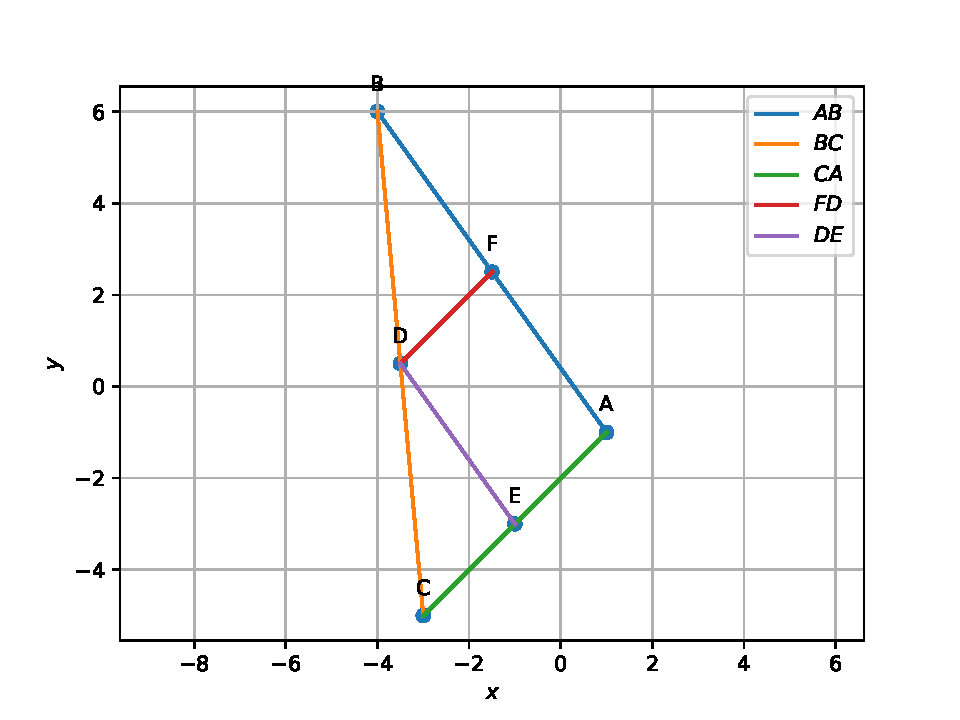
\includegraphics[width=0.75\columnwidth]{figs/triangle/pgm.pdf}
\caption{$AFDE$ forms a parallelogram in triangle ABC}
\label{fig:Triangle-pgm}
\end{figure}






















All codes for this section are available at
\begin{lstlisting}
	codes/triangle/sides.py
\end{lstlisting}
\end{enumerate}

\item If the points $\vec{A}(6,  1),  \vec{B}(8,  2),  \vec{C}(9,  4)$ and $\vec{D}(p,  3)$ are the vertices of a parallelogram,  taken in order,  find the value of $p$.
\label{10/7/0/10}
\item 
If $(1,  2),  (4,  y),  (x,  6)$ and $(3,  5)$ are the vertices of a parallelogram taken in order,  find $x$ and $y$.
\label{10/7/2/6}
\item The fourth vertex $\vec{D}$ of a parallelogram $ABCD$ whose three vertices are
	$\vec{A} (–2,  3),  \vec{B} (6,  7)$ and  $\vec{C} (8,  3)$ is
\item Verify if the points $\vec{A}(4, 3),  \vec{B}(6, 4), \vec{C}(5, -6)$  and  $\vec{D}(-3, 5)$ are the vertices of a parallelogram.
\item A girl walks 4 km towards west,  then she walks 3 km in a direction 30$^{\circ}$ east of north and stops. Determine the girl's displacement from her initial point of departure.\\
	\solution
		\iffalse
\documentclass[10pt]{article}
\usepackage{graphicx}
\def\inputGnumericTable{}
\usepackage[latin1]{inputenc}
\usepackage{fullpage}
\usepackage{color}
\usepackage{array}
\usepackage{longtable}
\usepackage{calc}
\usepackage{multirow}
\usepackage{hhline}
\usepackage{ifthen}
\usepackage{amsmath}
\usepackage[none]{hyphenat}
\usepackage{listings}
\usepackage[english]{babel}
\usepackage{siunitx}
\usepackage{caption}
\usepackage{booktabs}
\usepackage{array}
\usepackage{extarrows}
\usepackage{enumerate}
\usepackage{enumitem}
\usepackage{amsmath}
\usepackage{commath}
\usepackage{gensymb}
\usepackage{amssymb}
\usepackage{multicol}
%\usepackage[utf8]{inputenc}
\lstset{
 frame=single,
 breaklines=true
}
\usepackage{hyperref}
\usepackage[margin=0.65in]{geometry}	 
%\usepackage{exsheets}% also loads the `tasks' package
\usepackage{atbegshi}
\AtBeginDocument{\AtBeginShipoutNext{\AtBeginShipoutDiscard}}

%new macro definitions
\renewcommand{\labelenumi}{(\roman{enumi})}
\newcommand{\mydet}[1]{\ensuremath{\begin{vmatrix}#1\end{vmatrix}}}
\providecommand{\brak}[1]{\ensuremath{\left(#1\right)}}
\newcommand{\solution}{\noindent \textbf{Solution: }}
\newcommand{\myvec}[1]{\ensuremath{\begin{pmatrix}#1\end{pmatrix}}}
\newenvironment{amatrix}[1]{%
	\left(\begin{array}{@{}*{#1}{c}|c@{}}
}{%
	\end{array}\right)
}

\newcommand{\myaugvec}[2]{\ensuremath{\begin{amatrix}{#1}#2\end{amatrix}}}
\providecommand{\norm}[1]{\left\1Vert#1\right\rVert}
\let\vec\mathbf{}


%\SetEnumitemKey{twocol}{
% before=\raggedcolumns\begin{multicols}{2},
% after=\end{multicols}}
%\SetEnumitemKey{fourcol}{
% before=\raggedcolumns\begin{multicols}{4},
% after=\end{multicols}} 


\begin{document}
\begin{center}
\title{\textbf{TRIANGLES}}
\date{\vspace{-5ex}}
\maketitle
\end{center}
\section*{9$^{th}$Math - Chapter 7}
This is Problem-8 from Exercise 7.1\\\\


\section*{\large Construction:}
\fi
The input parameters for construction
	are available in Table \ref{tab:chapters/9/7/1/8/table}.
\begin{table}[H]
	\centering
	%\subimport{../chapters/9/7/1/8/tables/}{table.tex}
     %%%%%%%%%%%%%%%%%%%%%%%%%%%%%%%%%%%%%%%%%%%%%%%%%%%%%%%%%%%%%%%%%%%%%%
%%                                                                  %%
%%  This is the header of a LaTeX2e file exported from Gnumeric.    %%
%%                                                                  %%
%%  This file can be compiled as it stands or included in another   %%
%%  LaTeX document. The table is based on the longtable package so  %%
%%  the longtable options (headers, footers...) can be set in the   %%
%%  preamble section below (see PRAMBLE).                           %%
%%                                                                  %%
%%  To include the file in another, the following two lines must be %%
%%  in the including file:                                          %%
%%        \def\inputGnumericTable{}                                 %%
%%  at the beginning of the file and:                               %%
%%        \input{name-of-this-file.tex}                             %%
%%  where the table is to be placed. Note also that the including   %%
%%  file must use the following packages for the table to be        %%
%%  rendered correctly:                                             %%
%%    \usepackage[latin1]{inputenc}                                 %%
%%    \usepackage{color}                                            %%
%%    \usepackage{array}                                            %%
%%    \usepackage{longtable}                                        %%
%%    \usepackage{calc}                                             %%
%%    \usepackage{multirow}                                         %%
%%    \usepackage{hhline}                                           %%
%%    \usepackage{ifthen}                                           %%
%%  optionally (for landscape tables embedded in another document): %%
%%    \usepackage{lscape}                                           %%
%%                                                                  %%
%%%%%%%%%%%%%%%%%%%%%%%%%%%%%%%%%%%%%%%%%%%%%%%%%%%%%%%%%%%%%%%%%%%%%



%%  This section checks if we are begin input into another file or  %%
%%  the file will be compiled alone. First use a macro taken from   %%
%%  the TeXbook ex 7.7 (suggestion of Han-Wen Nienhuys).            %%
\def\ifundefined#1{\expandafter\ifx\csname#1\endcsname\relax}


%%  Check for the \def token for inputed files. If it is not        %%
%%  defined, the file will be processed as a standalone and the     %%
%%  preamble will be used.                                          %%
\ifundefined{inputGnumericTable}

%%  We must be able to close or not the document at the end.        %%
	\def\gnumericTableEnd{\end{document}}


%%%%%%%%%%%%%%%%%%%%%%%%%%%%%%%%%%%%%%%%%%%%%%%%%%%%%%%%%%%%%%%%%%%%%%
%%                                                                  %%
%%  This is the PREAMBLE. Change these values to get the right      %%
%%  paper size and other niceties.                                  %%
%%                                                                  %%
%%%%%%%%%%%%%%%%%%%%%%%%%%%%%%%%%%%%%%%%%%%%%%%%%%%%%%%%%%%%%%%%%%%%%%

	\documentclass[12pt%
			  %,landscape%
                    ]{report}
       \usepackage[latin1]{inputenc}
       \usepackage{fullpage}
       \usepackage{color}
       \usepackage{array}
       \usepackage{longtable}
       \usepackage{calc}
       \usepackage{multirow}
       \usepackage{hhline}
       \usepackage{ifthen}
       \usepackage{gensymb}
       \usepackage{graphicx}
\usepackage{amsmath}
\usepackage{mathtools}
\newcommand{\mydet}[1]{\ensuremath{\begin{vmatrix}#1\end{vmatrix}}}
\providecommand{\brak}[1]{\ensuremath{\left(#1\right)}}
\providecommand{\norm}[1]{\left\lVert#1\right\rVert}
\newcommand{\solution}{\noindent \textbf{Solution: }}
\newcommand{\myvec}[1]{\ensuremath{\begin{pmatrix}#1\end{pmatrix}}}
\let\vec\mathbf
	\begin{document}


%%  End of the preamble for the standalone. The next section is for %%
%%  documents which are included into other LaTeX2e files.          %%
\else

%%  We are not a stand alone document. For a regular able, we will %%
%%  have no preamble and only define the closing to mean nothing.   %%
    \def\gnumericTableEnd{}

%%  If we want landscape mode in an embedded document, comment out  %%
%%  the line above and uncomment the two below. The table will      %%
%%  begin on a new page and run in landscape mode.                  %%
%       \def\gnumericTableEnd{\end{landscape}}
%       \begin{landscape}


%%  End of the else clause for this file being \input.              %%
\fi

%%%%%%%%%%%%%%%%%%%%%%%%%%%%%%%%%%%%%%%%%%%%%%%%%%%%%%%%%%%%%%%%%%%%%%
%%                                                                  %%
%%  The rest is the gnumeric table, except for the closing          %%
%%  statement. Changes below will alter the table's appearance.     %%
%%                                                                  %%
%%%%%%%%%%%%%%%%%%%%%%%%%%%%%%%%%%%%%%%%%%%%%%%%%%%%%%%%%%%%%%%%%%%%%%
\providecommand{\gnumericmathit}[1]{#1} 
%%  Uncomment the next line if you would like your numbers to be in %%
%%  italics if they are italizised in the gnumeric table.           %%
%\renewcommand{\gnumericmathit}[1]{\mathit{#1}}
\providecommand{\gnumericPB}[1]%
{\let\gnumericTemp=\\#1\let\\=\gnumericTemp\hspace{0pt}}
 \ifundefined{gnumericTableWidthDefined}
        \newlength{\gnumericTableWidth}
        \newlength{\gnumericTableWidthComplete}
        \newlength{\gnumericMultiRowLength}
        \global\def\gnumericTableWidthDefined{}
 \fi
%% The following setting protects this code from babel shorthands.  %%
 \ifthenelse{\isundefined{\languageshorthands}}{}{\languageshorthands{english}}
%%  The default table format retains the relative column widths of  %%
%%  gnumeric. They can easily be changed to c, r or l. In that case %%
%%  you may want to comment out the next line and uncomment the one %%
%%  thereafter                                                      %%
\providecommand\gnumbox{\makebox[0pt]}
%%\providecommand\gnumbox[1][]{\makebox}

%% to adjust positions in multirow situations                       %%
\setlength{\bigstrutjot}{\jot}
\setlength{\extrarowheight}{\doublerulesep}

%%  The \setlongtables command keeps column widths the same across  %%
%%  pages. Simply comment out next line for varying column widths.  %%
\setlongtables

\setlength\gnumericTableWidth{%
	40pt+%
	35pt+%
	210pt+%
0pt}
\def\gumericNumCols{3}
\setlength\gnumericTableWidthComplete{\gnumericTableWidth+%
         \tabcolsep*\gumericNumCols*2+\arrayrulewidth*\gumericNumCols}
\ifthenelse{\lengthtest{\gnumericTableWidthComplete > \linewidth}}%
         {\def\gnumericScale{\ratio{\linewidth-%
                        \tabcolsep*\gumericNumCols*2-%
                        \arrayrulewidth*\gumericNumCols}%
{\gnumericTableWidth}}}%
{\def\gnumericScale{1}}

%%%%%%%%%%%%%%%%%%%%%%%%%%%%%%%%%%%%%%%%%%%%%%%%%%%%%%%%%%%%%%%%%%%%%%
%%                                                                  %%
%% The following are the widths of the various columns. We are      %%
%% defining them here because then they are easier to change.       %%
%% Depending on the cell formats we may use them more than once.    %%
%%                                                                  %%
%%%%%%%%%%%%%%%%%%%%%%%%%%%%%%%%%%%%%%%%%%%%%%%%%%%%%%%%%%%%%%%%%%%%%%

\ifthenelse{\isundefined{\gnumericColA}}{\newlength{\gnumericColA}}{}\settowidth{\gnumericColA}{\begin{tabular}{@{}p{40pt*\gnumericScale}@{}}x\end{tabular}}
\ifthenelse{\isundefined{\gnumericColB}}{\newlength{\gnumericColB}}{}\settowidth{\gnumericColB}{\begin{tabular}{@{}p{35pt*\gnumericScale}@{}}x\end{tabular}}
\ifthenelse{\isundefined{\gnumericColC}}{\newlength{\gnumericColC}}{}\settowidth{\gnumericColC}{\begin{tabular}{@{}p{65pt*\gnumericScale}@{}}x\end{tabular}}

\begin{longtable}[c]{%
	b{\gnumericColA}%
	b{\gnumericColB}%
	b{\gnumericColC}%
	}

%%%%%%%%%%%%%%%%%%%%%%%%%%%%%%%%%%%%%%%%%%%%%%%%%%%%%%%%%%%%%%%%%%%%%%
%%  The longtable options. (Caption, headers... see Goosens, p.124) %%
%	\caption{The Table Caption.}             \\	%
% \hline	% Across the top of the table.
%%  The rest of these options are table rows which are placed on    %%
%%  the first, last or every page. Use \multicolumn if you want.    %%

%%  Header for the first page.                                      %%
%	\multicolumn{3}{c}{The First Header} \\ \hline 
%	\multicolumn{1}{c}{colTag}	%Column 1
%	&\multicolumn{1}{c}{colTag}	%Column 2
%	&\multicolumn{1}{c}{colTag}	\\ \hline %Last column
%	\endfirsthead

%%  The running header definition.                                  %%
%	\hline
%	\multicolumn{3}{l}{\ldots\small\slshape continued} \\ \hline
%	\multicolumn{1}{c}{colTag}	%Column 1
%	&\multicolumn{1}{c}{colTag}	%Column 2
%	&\multicolumn{1}{c}{colTag}	\\ \hline %Last column
%	\endhead

%%  The running footer definition.                                  %%
%	\hline
%	\multicolumn{3}{r}{\small\slshape continued\ldots} \\
%	\endfoot

%%  The ending footer definition.                                   %%
%	\multicolumn{3}{c}{That's all folks} \\ \hline 
%	\endlastfoot
%%%%%%%%%%%%%%%%%%%%%%%%%%%%%%%%%%%%%%%%%%%%%%%%%%%%%%%%%%%%%%%%%%%%%%

\hhline{|-|-|-}
	 \multicolumn{1}{|p{\gnumericColA}|}%
	{\gnumericPB{\raggedright}\gnumbox[l]{\textbf{Symbol}}}
	&\multicolumn{1}{p{\gnumericColB}|}%
	{\gnumericPB{\raggedright}\gnumbox[l]{\textbf{Values}}}
	&\multicolumn{1}{p{\gnumericColC}|}%
	{\gnumericPB{\raggedright}\gnumbox[l]{\textbf{Description}}}
\\
\hhline{|---|}
	 \multicolumn{1}{|p{\gnumericColA}|}%
	{\gnumericPB{\raggedright}\gnumbox[l]{$r$}}
	&\multicolumn{1}{p{\gnumericColB}|}%
	{\gnumericPB{\raggedright}\gnumbox[l]{2}}
	&\multicolumn{1}{p{\gnumericColC}|}%
	{\gnumericPB{\raggedright}\gnumbox[l]{radius}}
\\
\hhline{|---|}
	 \multicolumn{1}{|p{\gnumericColA}|}%
	{\gnumericPB{\raggedright}\gnumbox[l]{$\vec{O}$}}
	&\multicolumn{1}{p{\gnumericColB}|}%
	{\gnumericPB{\raggedright}\gnumbox[l]{$\myvec{0\\0}$}}
	&\multicolumn{1}{p{\gnumericColC}|}%
	{\gnumericPB{\raggedright}\gnumbox[l]{center}}
\\
\hhline{|---|}
\end{longtable}

\ifthenelse{\isundefined{\languageshorthands}}{}{\languageshorthands{\languagename}}
\gnumericTableEnd%t

	\caption{}
	\label{tab:chapters/9/7/1/8/table}
\end{table}
Thus, 
\begin{align}
	\vec{A}=\myvec{0\\b},\,
	\vec{B}=\myvec{a\\0},\,
	\vec{C}=\myvec{0\\0}
\end{align}
yielding
\begin{align}
	\vec{M}&=\frac{\vec{A}+\vec{B}}{2}=\frac{1}{2}\myvec{a\\b}
\end{align}
Also, 
\begin{align}
	\vec{M}&=\frac{\vec{C}+\vec{D}}{2}\\
	\implies \vec{D}&=2\vec{M}-\vec{C}=\myvec{a\\b}
\end{align}
\iffalse
\solution
Given
\begin{align}
	\vec{M}&=\frac{\vec{A}+\vec{B}}{2}
	\label{eq:chapters/9/7/1/8/1}\\
	\vec{D}-\vec{M}&=\vec{C}-\vec{M}
	\label{eq:chapters/9/7/1/8/2}\\
	\angle ACB&=90\degree
\end{align}
\textbf{Proof:} From Figure \ref{fig:chapters/9/7/1/8/1}
\fi
Thus,
\begin{align}
	\brak{\vec{D}-\vec{B}}^{\top}\brak{\vec{B}-\vec{C}} &= \myvec{0 & b}\myvec{a\\0}=0\\
	\implies BD & \perp BC\\
\end{align}
Also, 
\begin{align}
	\norm{\vec{A}-\vec{B}}&=\norm{\myvec{-a\\b}}\\
	\norm{\vec{C}-\vec{D}}&=\norm{\myvec{-a\\-b}}\\
	\implies \norm{\vec{A}-\vec{B}} &= \norm{\vec{C}-\vec{D}}\\
	\text{ or, } AB &= CD
	\label{eq:chapters/9/7/1/8/3}	
\end{align}
From \eqref{eq:chapters/9/7/1/8/3}
\begin{align}
	\implies CM = \frac{1}{2}CD = \frac{1}{2}AB 
\end{align}
See Fig. 
\ref{fig:chapters/9/7/1/8/1}.
\begin{figure}[H]
	\begin{center}
		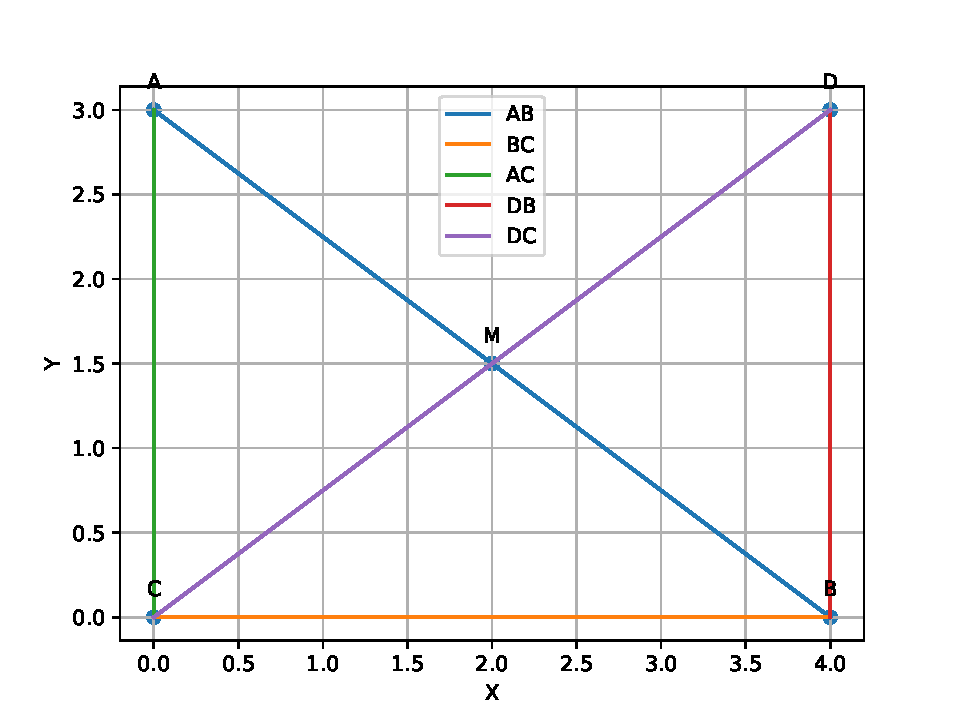
\includegraphics[width=0.75\columnwidth]{./chapters/9/7/1/8/figs/fig.pdf}
	\end{center}
\caption{}
\label{fig:chapters/9/7/1/8/1}
\end{figure}


\item $(-1, 2, 1),  (1, -2, 5),  (4, -7, 8)$ and $(2, -3, 4)$ are the vertices of a parallelogram.
\item Three vertices of a parallelogram $ABCD$ are $\vec{A}(3, -1, 2),  \vec{B}(1, -2, 4)$ and $\vec{C}(-1, 1, 2)$. Find the coordinates of the fourth vertex.
\item If the origin is the centroid of the triangle $PQR$ with vertices $\vec{P}(2a, 2, 6),  \vec{Q}(-4, 3b, -10)$ and $R(8, 14, 2c)$,  then find the values of $a,  b$ and $c$.
\item Find the slope of lines
\begin{enumerate}
\item  Passing through the points $(3, -2)$ and $(-1, 4)$
\item  Passing through the points $(3, -2)$ and $(7, -2)$
\item  passing through the points $(3, -2)$ and $(3, 4)$	
\item  Making inclination of $60\degree$ with the positive direction of x-axis.
\end{enumerate}
\item The centroid of a triangle $ABC$ is at the point $(1, 1, 1)$. If the coordinates of $\vec{A}$ and $\vec{B}$ are $(3, -5, 7)$ and $(-1, 7, -6)$,  respectively find the coordinates of the point $\vec{C}$.
\item Represent graphically a displacement of $40$ km,  $30\degree$ west of south.
	\item Rain is falling vertically with a speed of 35 $m s^{-1}$
. Winds starts blowing after sometime with a speed of 12 $m s^{-1}$ in
east to west direction. In which direction should a boy waiting at a bus stop hold his umbrella ?
%
\item A motorboat is racing towards north at 25 km/h and the water current in that region is 10 km/h in the direction of 60$\degree$ east of south. Find the resultant velocity of the boat.
\item Rain is falling vertically with a speed of 35 $m s^{-1}$
. A woman rides a bicycle with a speed of 12 $ms^{-1}$ in east to west
direction. What is the direction in which she should hold her umbrella ?
\item Rain is falling vertically with a speed of 30 $m s^{-1}$. A woman rides a bicycle with a speed  of 10 $m s^{-1}$ in the north to south direction. What is the direction in which she should
hold her umbrella?
\item A man can swim with a speed of 4.0 km/h in still water. How long does he take to cross a river 1.0 km wide if the river flows steadily at 3.0 km/h and he makes his strokes normal to the river current? How far down the river does he go when he reaches the other bank ?
\item In a harbour,  wind is blowing at the speed of 72 km/h and the flag on the mast of a boat anchored in the harbour flutters along the N-E direction. If the boat starts moving at a speed of 51 km/h to the north,  what is the direction of the flag on the mast of the boat ?
\item In which quadrant or on which axis do each of the points (-2, 4), (3, -1), (-1, 0), (1, 2) and (-3, -5) lie? Verify your answer by locating them on the Cartesian plane.
\item Plot the points $(x, y)$ given in 
\tabref{table:Table of values}.
\begin{table}[H]
	\centering
\begin{tabular}{|c|c|c|c|c|c|}
\hline	
x & -2 & -1 & 0 & 1 & 3\\
\hline
y & 8 & 7 & -1.25 & 3 & -1\\
\hline
\end{tabular}
\caption{}
\label{table:Table of values}
\end{table}
\end{enumerate}

\subsection{CBSE}
\begin{enumerate}[label=\thesubsection.\arabic*, ref=\thesubsection.\theenumi]
	\item 		Find the values of $x$ and $y$ so that the vectors
$2\hat{i}+3\hat{j}$
and 
$x\hat{i}+y\hat{j}$
are equal.
\\
\solution
%\renewcommand{\theequation}{\theenumi}
\begin{enumerate}[label=\thesubsection.\arabic*.,ref=\thesubsection.\theenumi]
%\numberwithin{equation}{enumi}
\item The direction vector of $AB$ is defined as
		\begin{align}
			\vec{B}-
			\vec{A}
		\end{align}
Find the direction vectors of $AB, BC$ and $CA$.
\\
\solution 
\begin{enumerate} 
\item  The Direction vector of $AB$ is 
	\begin{align}  \vec{B} - \vec{A} 
		=\myvec{ -4\\ 6 } - \myvec{ 1\\ -1 }
 = \myvec{ -4 - 1\\ 6 - (-1) } = \myvec{ -5\\ 7 }
		\label{eq:app-geo-dir-vec-ab}
 \end{align}
\item The Direction vector of $BC$ is
	\begin{align} \vec{C} - \vec{B}=\myvec{ -3\\ -5} - \myvec{ -4\\ 6 }
 = \myvec{ -3 - (-4)\\ -5 - 6 } = \myvec{1\\ -11 }
		\label{eq:app-geo-dir-vec-bc}
  \end{align}
  \item  The Direction vector of $CA$  is
	  \begin{align}  \vec{A} - \vec{C} =\myvec{ 1\\ -1 }-\myvec{ -3\\ -5}
 = \myvec{ 1 - (-3)\\ -1 - (-5) } = \myvec{ 4\\ 4 }
		\label{eq:app-geo-dir-vec-ca}
  \end{align}
 \end{enumerate}
%	\solution 
\begin{enumerate} 
\item  The Direction vector of $AB$ is 
	\begin{align}  \vec{B} - \vec{A} 
		=\myvec{ -4\\ 6 } - \myvec{ 1\\ -1 }
 = \myvec{ -4 - 1\\ 6 - (-1) } = \myvec{ -5\\ 7 }
		\label{eq:geo-dir-vec-ab}
 \end{align}
\item The Direction vector of $BC$ is
	\begin{align} \vec{C} - \vec{B}=\myvec{ -3\\ -5} - \myvec{ -4\\ 6 }
 = \myvec{ -3 - (-4)\\ -5 - 6 } = \myvec{1\\ -11 }
		\label{eq:geo-dir-vec-bc}
  \end{align}
  \item  The Direction vector of $CA$  is
	  \begin{align}  \vec{A} - \vec{C} =\myvec{ 1\\ -1 }-\myvec{ -3\\ -5}
 = \myvec{ 1 - (-3)\\ -1 - (-5) } = \myvec{ 4\\ 4 }
		\label{eq:geo-dir-vec-ca}
  \end{align}
 \end{enumerate}


	\item The length of side $BC$ is 
		\label{prob:side-length}
		\begin{align}
			c = \norm{\vec{B}-\vec{A}} \triangleq \sqrt{\brak{\vec{B}-\vec{A}}^{\top}\brak{\vec{B}-\vec{A}}}
		\end{align}
		where
		\begin{align}
			\vec{A}^{\top}\triangleq\myvec{1 & -1}
		\end{align}
		Similarly, 
		\begin{align}
b = \norm{\vec{C}-\vec{B}},\,
a = \norm{\vec{A}-\vec{C}}
		\end{align}
		Find $a, b, c$.
\begin{enumerate}
	\item 
	From 	
		\eqref{eq:app-geo-dir-vec-ab},
\begin{align}
\vec{A}-\vec{B} &= \myvec{5\\-7}, \\
\implies 	c &= 	\norm{\vec{B}-\vec{A}} = \norm{\vec{A}-\vec{B}} 
	\\
	&= \sqrt{\myvec{5 & -7}\myvec{5\\-7}}
= \sqrt{\brak{5}^2 +\brak{7}^2}\\
	&=\sqrt{74}
		\label{eq:app-geo-norm-ab}
\end{align}
	\item Similarly, from 
		\eqref{eq:app-geo-dir-vec-bc},
\begin{align}
	a &= \norm{\vec{B}-\vec{C}} 
	= \sqrt{\myvec{-1 & 11}\myvec{-1\\11}}
\\
&= \sqrt{\brak{1}^2+\brak{11}^2}
	= \sqrt{122}
		\label{eq:app-geo-norm-bc}
\end{align}
and
		from 		\eqref{eq:app-geo-dir-vec-ca},
	\item 
		\begin{align}
			b &= \norm{\vec{A}-\vec{C}} = \sqrt{\myvec{4 & 4}\myvec{4\\4}}
\\
&= \sqrt{\brak{4}^2+\brak{4}^2}
	=\sqrt{32}
		\label{eq:app-geo-norm-ca}
\end{align}
\end{enumerate}
%  \\            
  %\\ \solution 
\begin{align}
    \vec{A}-\vec{F}&=\myvec{1\\-1}-\myvec{\frac{-3}{2}\\\frac{5}{2}}
    =\myvec{\frac{5}{2}\\\frac{-7}{2}}
    \\
    \vec{E}-\vec{D}&=\myvec{-1\\-3}-\myvec{\frac{-7}{2}\\\frac{1}{2}}
    =\myvec{\frac{5}{2}\\\frac{-7}{2}}
    \\
	\implies	\vec{A}-\vec{F} &= \vec{E}-\vec{D}
\end{align}
See \figref{fig:Triangle-pgm}, 
\begin{figure}
\centering
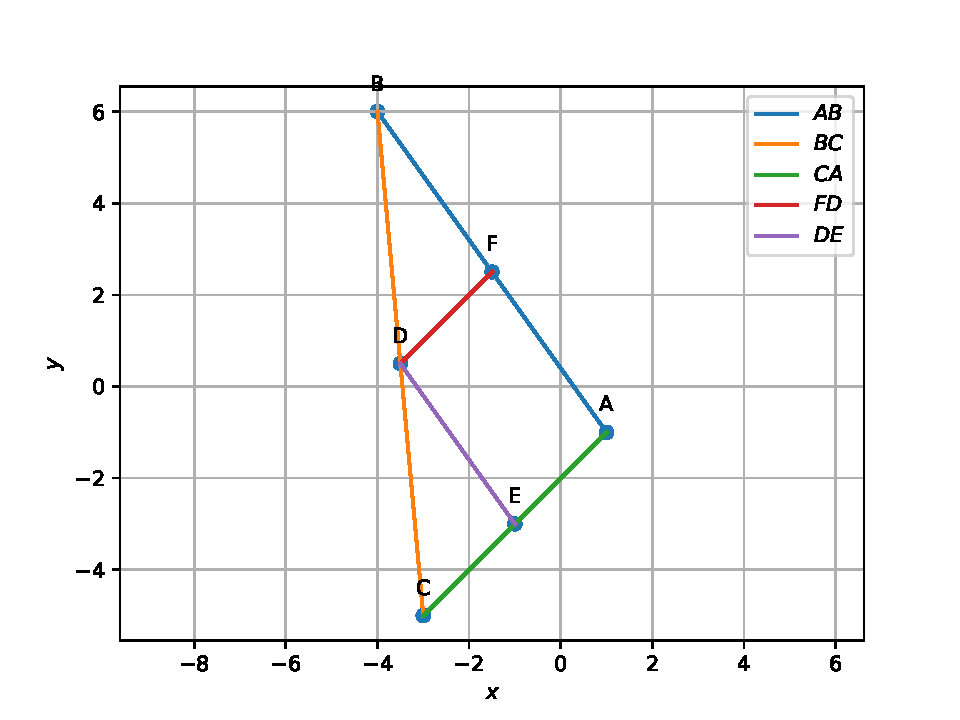
\includegraphics[width=0.75\columnwidth]{figs/triangle/pgm.pdf}
\caption{$AFDE$ forms a parallelogram in triangle ABC}
\label{fig:Triangle-pgm}
\end{figure}






















\item   Points $\vec{A}, \vec{B}, \vec{C}$ are defined to be collinear if 
		\begin{align}
			\label{eq:app-app-line-rank}
			\rank{\myvec{1 & 1 & 1 \\ \vec{A}& \vec{B}&\vec{C}}} = 2
		\end{align}
Are the given points in
			\eqref{eq:app-tri-pts}
collinear?
\\
\solution 
From 
			\eqref{eq:app-tri-pts},
\begin{align}
    \label{eq:app-1.1.3,2}
\myvec{
    1 & 1 & 1\\
    \vec{A} & \vec{B} & \vec{C} \\
    } 
    =
    %\label{eq:app-matthrowoperations}
    \myvec{
    1 & 1 & 1
    \\
    1 & -4 & -3
    \\
    -1 & 6 & -5
    }
     \xleftrightarrow[]{R_3 \leftarrow R_3+R_2}
    \myvec{
    1 & 1 & 1
    \\
    1 & -4 & -3
    \\
    0 & 2 & -8 
    }
    \\
     \xleftrightarrow[]{R_2\leftarrow R_1-R_2}
    \myvec{
    1 & 1 & 1
    \\
    0 & 5 & 4
    \\
    0 & 2 & -8 
    }
     \xleftrightarrow[]{R_3\leftarrow R_3-\frac{2}{5}R_2}
    \myvec{
    1 & 1 & 1
    \\
    0 & 5 & 4
    \\
    0 & 0 & \frac{-48}{5}
    }
\end{align}
There are no zero rows. So,
\begin{align}
    \text{rank}\myvec{
    1 & 1 & 1\\
    \vec{A} & \vec{B} & \vec{C} \\
    } &= 3 
\end{align}  
Hence,  the points $\vec{A},\vec{B},\vec{C}$ are not collinear. 
This is visible in 
\figref{fig1:Triangle}.
\begin{figure}[H]
\centering
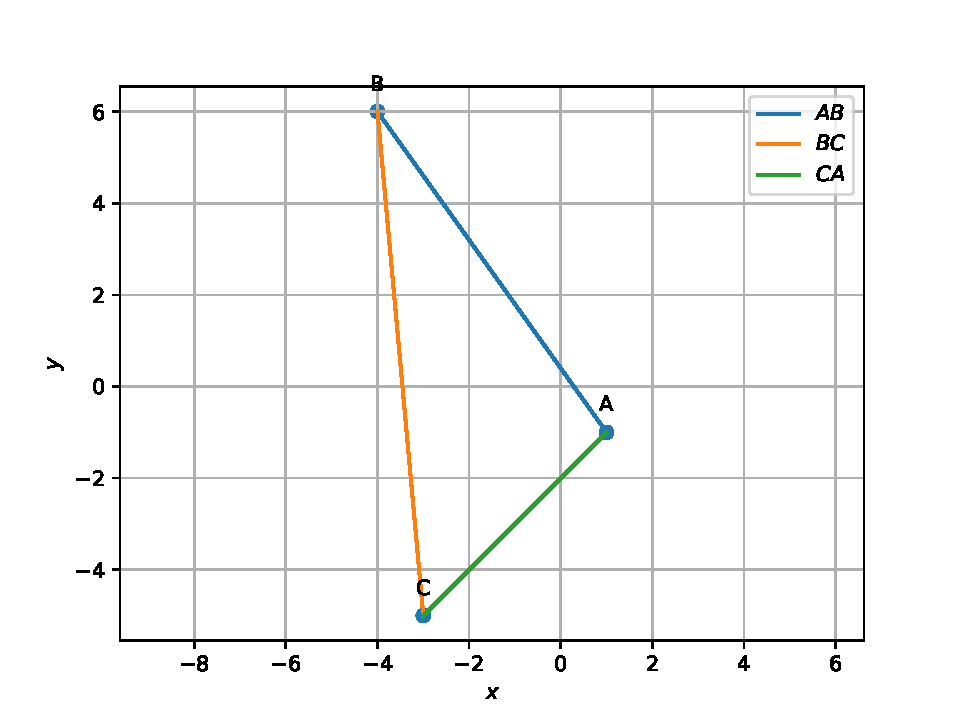
\includegraphics[width=0.75\columnwidth]{figs/triangle/vector.pdf}
\caption{$\triangle ABC$}
\label{fig1:Triangle}
\end{figure}
% \\		\\ \solution 
\begin{align}
    \vec{A}-\vec{F}&=\myvec{1\\-1}-\myvec{\frac{-3}{2}\\\frac{5}{2}}
    =\myvec{\frac{5}{2}\\\frac{-7}{2}}
    \\
    \vec{E}-\vec{D}&=\myvec{-1\\-3}-\myvec{\frac{-7}{2}\\\frac{1}{2}}
    =\myvec{\frac{5}{2}\\\frac{-7}{2}}
    \\
	\implies	\vec{A}-\vec{F} &= \vec{E}-\vec{D}
\end{align}
See \figref{fig:Triangle-pgm}, 
\begin{figure}
\centering
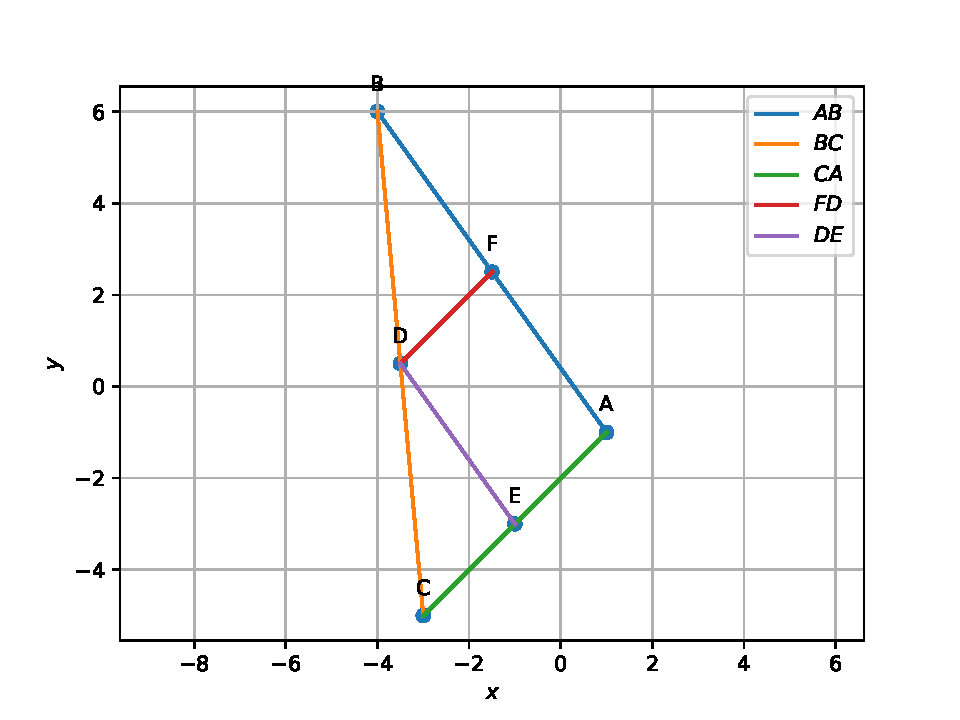
\includegraphics[width=0.75\columnwidth]{figs/triangle/pgm.pdf}
\caption{$AFDE$ forms a parallelogram in triangle ABC}
\label{fig:Triangle-pgm}
\end{figure}






















\item The parameteric form of the equation  of $AB$ is 
		\begin{align}
			\label{eq:app-geo-param}
			\vec{x}=\vec{A}+k\vec{m} \quad k \ne 0,
		\end{align}
		where
		\begin{align}
\vec{m}=\vec{B}-\vec{A}
		\end{align}
is the direction vector of $AB$.
Find the parameteric equations of $AB, BC$ and $CA$.
\\
\solution
From 
			\eqref{eq:app-geo-param} and
		\eqref{eq:app-geo-dir-vec-ab},
the parametric equation for $AB$ is given by
\begin{align}
AB: \vec{x} = &\myvec{1\\-1} + k \myvec{-5\\7}
\end{align}
Similarly, from 
		\eqref{eq:app-geo-dir-vec-bc} and
		\eqref{eq:app-geo-dir-vec-ca},
\begin{align}
BC: \vec{x} = &\myvec{-4\\6} + k \myvec{1\\-11}\\
CA: \vec{x} = &\myvec{-3\\-5} + k \myvec{4\\4}
\end{align}

%		\\ \solution 
\begin{align}
    \vec{A}-\vec{F}&=\myvec{1\\-1}-\myvec{\frac{-3}{2}\\\frac{5}{2}}
    =\myvec{\frac{5}{2}\\\frac{-7}{2}}
    \\
    \vec{E}-\vec{D}&=\myvec{-1\\-3}-\myvec{\frac{-7}{2}\\\frac{1}{2}}
    =\myvec{\frac{5}{2}\\\frac{-7}{2}}
    \\
	\implies	\vec{A}-\vec{F} &= \vec{E}-\vec{D}
\end{align}
See \figref{fig:Triangle-pgm}, 
\begin{figure}
\centering
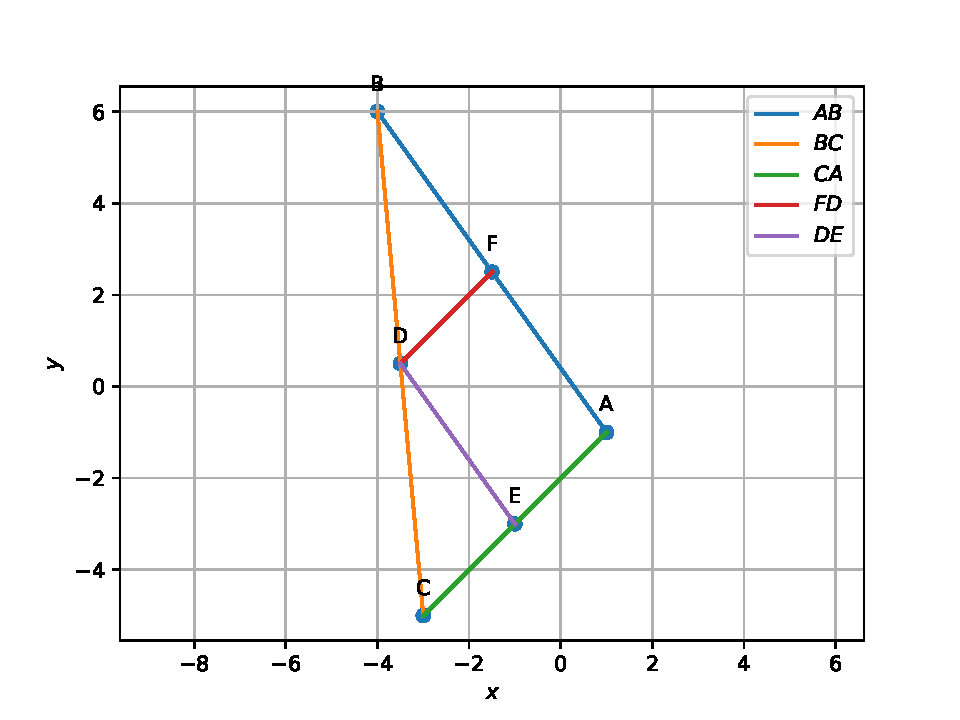
\includegraphics[width=0.75\columnwidth]{figs/triangle/pgm.pdf}
\caption{$AFDE$ forms a parallelogram in triangle ABC}
\label{fig:Triangle-pgm}
\end{figure}






















\item The normal form of the equation of $AB$  is 
		\begin{align}
			\label{eq:app-geo-normal}
			\vec{n}^{\top}\brak{	\vec{x}-\vec{A}} = 0
		\end{align}
		where 
		\begin{align}
			\vec{n}^{\top}\vec{m}&=\vec{n}^{\top}\brak{\vec{B}-\vec{A}} = 0
			\\
			\text{or, } \vec{n}&=\myvec{0 & 1 \\ -1 & 0} \vec{m}
			\label{eq:app-geo-norm-vec}
		\end{align}
Find the normal form of the equations of $AB, BC$ and $CA$.
\\
\solution
\begin{enumerate}
	\item
From
		\eqref{eq:app-geo-dir-vec-bc}, 
the direction vector of side $\vec{BC}$ is
\begin{align}
\vec{m}
	&=\myvec{1\\-11}
	\\
\implies \vec{n} &= \myvec{0 & 1\\
  -1 & 0}\myvec{1\\-11}
 = \myvec{-11\\-1}
		\label{eq:app-geo-norm-vec-bc}
\end{align}
from 
			\eqref{eq:app-geo-norm-vec}.
Hence, from 
			\eqref{eq:app-geo-normal},
the normal equation of side $BC$ is 
\begin{align}
	\vec{n}^{\top}\brak{	\vec{x}-\vec{B}} &= 0
			\\
\implies    \myvec{-11 & -1}\vec{x}&=\myvec{-11 & -1}\myvec{-4\\6}\\
    \implies
BC: \quad    \myvec{11 & 1}\vec{x}&=-38
\end{align}
\item Similarly, for $AB$,
from 
		\eqref{eq:app-geo-dir-vec-ab}, 
\begin{align}
	\vec{m} &= \myvec{-5\\7}
	\\
\implies        \vec{n} 
                &= \myvec{0&1\\-1&0}\myvec{-5\\7}
                = \myvec{7\\5}
		\label{eq:app-geo-norm-vec-ab}
\end{align}
and 
\begin{align}
	\vec{n}^{\top}\brak{	\vec{x}-\vec{A}} &= 0
	\\
	\implies
                AB: \quad  \vec{n}^{\top}\vec{x} &= \myvec{7&5}\myvec{1\\-1}\\    
       \implies\myvec{7&5}\vec{x} &= 2
\end{align}
\item For 
$CA$, 
from 
		\eqref{eq:app-geo-dir-vec-ca}, 
\begin{align}
\vec{m} &= \myvec{1 \\ 1}
\\
		\label{eq:app-geo-norm-vec-ca}
\implies \vec{n} 
&= \myvec{0&1 \\ -1&0}\myvec{1 \\ 1}
= \myvec{1 \\ -1}\\
\\
\implies	\vec{n}^{\top}\brak{	\vec{x}-\vec{C}} &= 0
\\
\implies \myvec{1&-1}{\vec{x}} &= \myvec{1&-1}\myvec{-3 \\ -5} 
= 2 
\end{align}
\end{enumerate}

%\begin{enumerate}
	\item
From
		\eqref{eq:geo-dir-vec-bc}, 
the direction vector of side $\vec{BC}$ is
\begin{align}
\vec{m}
	&=\myvec{1\\-11}
	\\
\implies \vec{n} &= \myvec{0 & 1\\
  -1 & 0}\myvec{1\\-11}
 = \myvec{-11\\-1}
		\label{eq:geo-norm-vec-bc}
\end{align}
from 
			\eqref{eq:geo-norm-vec}.
Hence, from 
			\eqref{eq:geo-normal},
the normal equation of side $BC$ is 
\begin{align}
	\vec{n}^{\top}\brak{	\vec{x}-\vec{B}} &= 0
			\\
\implies    \myvec{-11 & -1}\vec{x}&=\myvec{-11 & -1}\myvec{-4\\6}\\
    \implies
BC: \quad    \myvec{11 & 1}\vec{x}&=-38
\end{align}
\item Similarly, for $AB$,
from 
		\eqref{eq:geo-dir-vec-ab}, 
\begin{align}
	\vec{m} &= \myvec{-5\\7}
	\\
\implies        \vec{n} 
                &= \myvec{0&1\\-1&0}\myvec{-5\\7}
                = \myvec{7\\5}
		\label{eq:geo-norm-vec-ab}
\end{align}
and 
\begin{align}
	\vec{n}^{\top}\brak{	\vec{x}-\vec{A}} &= 0
	\\
	\implies
                AB: \quad  \vec{n}^{\top}\vec{x} &= \myvec{7&5}\myvec{1\\-1}\\    
       \implies\myvec{7&5}\vec{x} &= 2
\end{align}
\item For 
$CA$, 
from 
		\eqref{eq:geo-dir-vec-ca}, 
\begin{align}
\vec{m} &= \myvec{1 \\ 1}
\\
		\label{eq:geo-norm-vec-ca}
\implies \vec{n} 
&= \myvec{0&1 \\ -1&0}\myvec{1 \\ 1}
= \myvec{1 \\ -1}\\
\\
\implies	\vec{n}^{\top}\brak{	\vec{x}-\vec{C}} &= 0
\\
\implies \myvec{1&-1}{\vec{x}} &= \myvec{1&-1}\myvec{-3 \\ -5} 
= 2 
\end{align}
\end{enumerate}


\item The area of $\triangle ABC$ is defined as
		\begin{align}
			\label{eq:app-tri-area-cross}
			\frac{1}{2}\norm{{\brak{\vec{A}-\vec{B}}\times \brak{\vec{A}-\vec{C}}}}
		\end{align}
		where
		\begin{align}
			\vec{A}\times\vec{B} \triangleq \mydet{1 & -4 \\-1 & 6}
		\end{align}
		Find the area of $\triangle ABC$.\\
\solution
From
		\eqref{eq:app-geo-dir-vec-ab}
		and
		\eqref{eq:app-geo-dir-vec-ca},
\begin{align}
	\vec{A}-\vec{B}=\myvec{5\\-7},
	\vec{A}-\vec{C}&=\myvec{4\\4}\\
\implies (\vec{A}-\vec{B})\times(\vec{A}-\vec{C}) &=\mydet{5 & 4\\-7 & 4}\\
&=5\times 4-4\times (-7)\\&=48\\
\implies\frac{1}{2}\norm{(\vec{A}-\vec{B})\times(\vec{A}-\vec{C})}&=\frac{48}{2}=24
\end{align}
which is the desired area.

%  		\\ \solution 
\begin{align}
    \vec{A}-\vec{F}&=\myvec{1\\-1}-\myvec{\frac{-3}{2}\\\frac{5}{2}}
    =\myvec{\frac{5}{2}\\\frac{-7}{2}}
    \\
    \vec{E}-\vec{D}&=\myvec{-1\\-3}-\myvec{\frac{-7}{2}\\\frac{1}{2}}
    =\myvec{\frac{5}{2}\\\frac{-7}{2}}
    \\
	\implies	\vec{A}-\vec{F} &= \vec{E}-\vec{D}
\end{align}
See \figref{fig:Triangle-pgm}, 
\begin{figure}
\centering
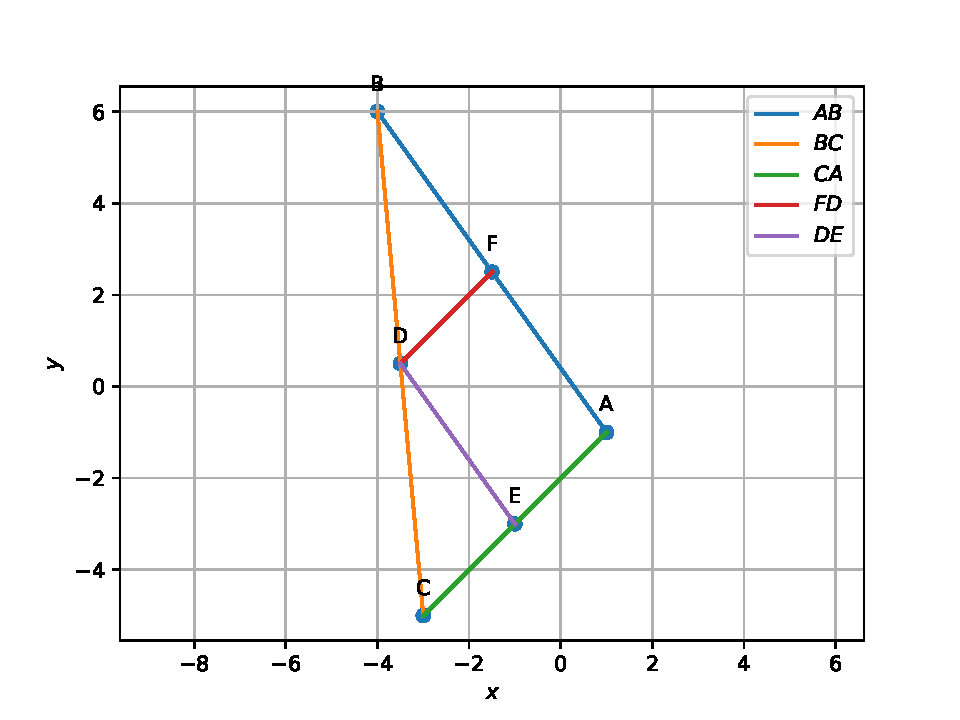
\includegraphics[width=0.75\columnwidth]{figs/triangle/pgm.pdf}
\caption{$AFDE$ forms a parallelogram in triangle ABC}
\label{fig:Triangle-pgm}
\end{figure}






















	\item Find the angles $A, B, C$ if 
%    \label{prop:angle2d}
  \begin{align}
    \label{eq:app-angle2d}
			\cos A \triangleq 
\frac{\brak{\vec{B}-\vec{A}}^{\top}{\vec{C}-\vec{A}}}{\norm{\vec{B}-\vec{A}}\norm{\vec{C}-\vec{A}}}
  \end{align}\\
  \solution
\begin{enumerate}
	\item From 
		\eqref{eq:app-geo-dir-vec-ab},
		\eqref{eq:app-geo-dir-vec-ca},
		\eqref{eq:app-geo-norm-ab}
		and
		\eqref{eq:app-geo-norm-ca}
\begin{align}
	(\vec{B}-\vec{A})^{\top}(\vec{C}-\vec{A})&=\myvec{-5&7}\myvec{-4\\-4}\\
	&=-8
	\\
	\implies
	\cos{A}&= \frac{-8}{\sqrt{74} \sqrt{32}}
	= \frac{-1}{\sqrt{37}}\\
	\implies A&=\cos^{-1}{\frac{-1}{\sqrt{37}}}
\end{align}
	\item From 
		\eqref{eq:app-geo-dir-vec-ab},
		\eqref{eq:app-geo-dir-vec-bc},
		\eqref{eq:app-geo-norm-ab}
		and
		\eqref{eq:app-geo-norm-bc}
\begin{align}
	(\vec{C}-\vec{B})^{\top}(\vec{A}-\vec{B})&=\myvec{1&-11}\myvec{5\\-7}\\
	&= 82
	\\
	\implies
	\cos{B}&= \frac{82}{\sqrt{74} \sqrt{122}}
	= \frac{41}{\sqrt{2257}}\\
	\implies B&=\cos^{-1}{\frac{41}{\sqrt{2257}}}
\end{align}
	\item From 
		\eqref{eq:app-geo-dir-vec-bc},
		\eqref{eq:app-geo-dir-vec-ca},
		\eqref{eq:app-geo-norm-bc}
		and
		\eqref{eq:app-geo-norm-ca}
\begin{align}
	(\vec{A}-\vec{C})^{\top}(\vec{B}-\vec{C})&=\myvec{4&4}\myvec{-1\\11}\\
	&=40
	\\
\implies	\cos{C}&= \frac{40}{\sqrt{32} \sqrt{122}}
	= \frac{5}{\sqrt{61}}\\
	\implies C&=\cos^{-1}{\frac{5}{\sqrt{61}}}
\end{align}

\end{enumerate}
%  	\\ \solution 
\begin{align}
    \vec{A}-\vec{F}&=\myvec{1\\-1}-\myvec{\frac{-3}{2}\\\frac{5}{2}}
    =\myvec{\frac{5}{2}\\\frac{-7}{2}}
    \\
    \vec{E}-\vec{D}&=\myvec{-1\\-3}-\myvec{\frac{-7}{2}\\\frac{1}{2}}
    =\myvec{\frac{5}{2}\\\frac{-7}{2}}
    \\
	\implies	\vec{A}-\vec{F} &= \vec{E}-\vec{D}
\end{align}
See \figref{fig:Triangle-pgm}, 
\begin{figure}
\centering
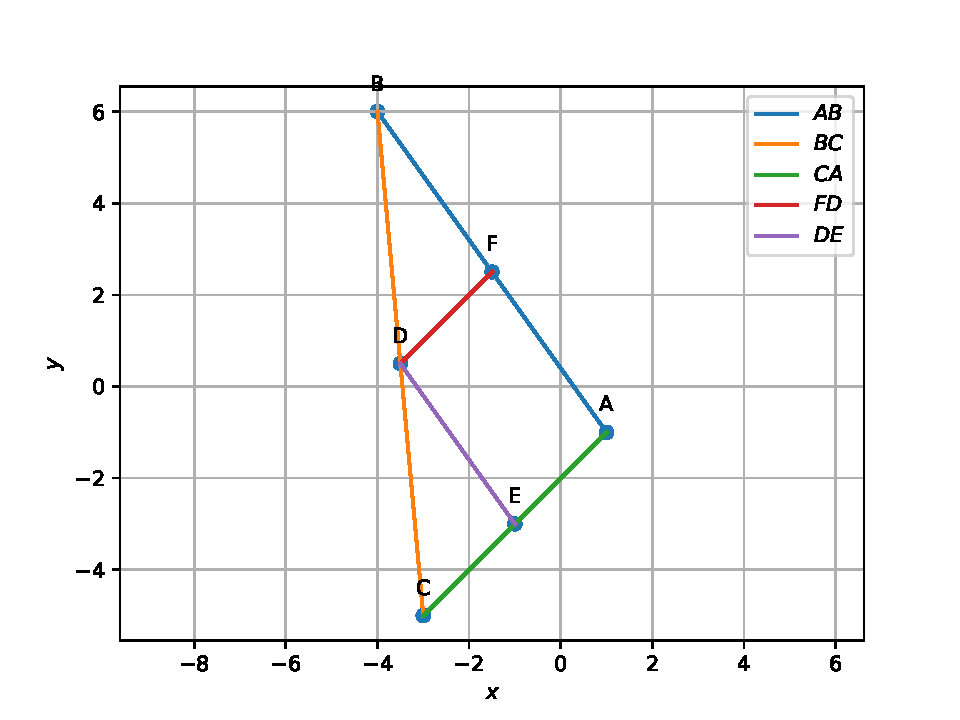
\includegraphics[width=0.75\columnwidth]{figs/triangle/pgm.pdf}
\caption{$AFDE$ forms a parallelogram in triangle ABC}
\label{fig:Triangle-pgm}
\end{figure}






















All codes for this section are available at
\begin{lstlisting}
	codes/triangle/sides.py
\end{lstlisting}
\end{enumerate}

\item Find the values of $x, y, z$ so that the vectors 
$x\hat{i}+2\hat{j}+z\hat{k}$
and 
$2\hat{i}+y\hat{j}+\hat{k}$
are equal.
\item Find the sum of the vectors $\vec{a}=\hat{i}-2\hat{j}+\hat{k}$,  $\vec{b}=-2\hat{i}+4\hat{j}+5\hat{k}$ and $\vec{c}=\hat{i}-6\hat{j}-7\hat{k}$.
\item Find the slope of a line,  which passes through the origin and the mid point of the line segment joining the points $\vec{P}$(0, -4) and $\vec{B}$(8, 0).
\label{chapters/11/10/1/5}
	\\
	\solution
The direction vector
\begin{align}
	\vec{B}-\vec{A}
	=
	\myvec{
  h-x_1\\
  k-y_1
  }
   \equiv
	\myvec{
1\\
	\frac{ k-y_1}{h-x_1}
  }
  \\
	\implies m = 
	\frac{ k-y_1}{h-x_1},
\end{align}
yielding the desired result.

\item Find the angle between x-axis and the line joining points (3, -1) and (4, -2).
\label{chapters/11/10/1/10}
\\
\solution 
The direction vector
\begin{align}
	\vec{B}-\vec{A}
	=
	\myvec{
  h-x_1\\
  k-y_1
  }
   \equiv
	\myvec{
1\\
	\frac{ k-y_1}{h-x_1}
  }
  \\
	\implies m = 
	\frac{ k-y_1}{h-x_1},
\end{align}
yielding the desired result.

\item A line passes through $\vec{A}(x_1, y_1)$ and $\vec{B}(h, k)$. If slope of the line is m,  show that $(k-y_1)=m(h-x_1)$.
\label{chapters/11/10/1/12}
\\
\solution 
The direction vector
\begin{align}
	\vec{B}-\vec{A}
	=
	\myvec{
  h-x_1\\
  k-y_1
  }
   \equiv
	\myvec{
1\\
	\frac{ k-y_1}{h-x_1}
  }
  \\
	\implies m = 
	\frac{ k-y_1}{h-x_1},
\end{align}
yielding the desired result.

\item
Show that the line through the points \brak{4, 7, 8}, \brak{2, 3, 4} is parallel to the line through the points \brak{-1, -2, 1}, \brak{1, 2, 5}.
	\label{12.11.2.3}
\\
\solution
	\begin{align}
\myvec{4 \\ 7 \\ 8}- \myvec{2 \\ 3 \\ 4}= \myvec{-1 \\ -2 \\ 1}- \myvec{1 \\ 2 \\ 5}
\equiv \myvec{2\\4\\4}
\end{align}
which means that the given lines have the same direction vector and are hence parallel.

\item The vector having intial and terminal points as (-2, 5, 0) and (3, 7, 4), respectively is
\solution
The desired vector is
\begin{align}
	\myvec{3 \\ 7 \\ 4}
	-\myvec{-2 \\ 5 \\ 0} = 
	\myvec{5 \\ 2 \\ 4}  
\end{align}
\item Find the vector joining the points $\vec{P}\brak{2, 3, 0}$ and $\vec{Q}\brak{-1, -2, -4}$ directed from $\vec{P}$ to $\vec{Q}$.
\item Without using distance formula,  show that points $\vec{A}(– 2,  – 1),  \vec{B}(4,  0),  \vec{C}(3,  3)$ and $\vec{D}(–3,  2)$ are the vertices of a parallelogram.
\label{chapters/11/10/1/9}
\\
\solution
%\renewcommand{\theequation}{\theenumi}
\begin{enumerate}[label=\thesubsection.\arabic*.,ref=\thesubsection.\theenumi]
%\numberwithin{equation}{enumi}
\item The direction vector of $AB$ is defined as
		\begin{align}
			\vec{B}-
			\vec{A}
		\end{align}
Find the direction vectors of $AB, BC$ and $CA$.
\\
\solution 
\begin{enumerate} 
\item  The Direction vector of $AB$ is 
	\begin{align}  \vec{B} - \vec{A} 
		=\myvec{ -4\\ 6 } - \myvec{ 1\\ -1 }
 = \myvec{ -4 - 1\\ 6 - (-1) } = \myvec{ -5\\ 7 }
		\label{eq:app-geo-dir-vec-ab}
 \end{align}
\item The Direction vector of $BC$ is
	\begin{align} \vec{C} - \vec{B}=\myvec{ -3\\ -5} - \myvec{ -4\\ 6 }
 = \myvec{ -3 - (-4)\\ -5 - 6 } = \myvec{1\\ -11 }
		\label{eq:app-geo-dir-vec-bc}
  \end{align}
  \item  The Direction vector of $CA$  is
	  \begin{align}  \vec{A} - \vec{C} =\myvec{ 1\\ -1 }-\myvec{ -3\\ -5}
 = \myvec{ 1 - (-3)\\ -1 - (-5) } = \myvec{ 4\\ 4 }
		\label{eq:app-geo-dir-vec-ca}
  \end{align}
 \end{enumerate}
%	\solution 
\begin{enumerate} 
\item  The Direction vector of $AB$ is 
	\begin{align}  \vec{B} - \vec{A} 
		=\myvec{ -4\\ 6 } - \myvec{ 1\\ -1 }
 = \myvec{ -4 - 1\\ 6 - (-1) } = \myvec{ -5\\ 7 }
		\label{eq:geo-dir-vec-ab}
 \end{align}
\item The Direction vector of $BC$ is
	\begin{align} \vec{C} - \vec{B}=\myvec{ -3\\ -5} - \myvec{ -4\\ 6 }
 = \myvec{ -3 - (-4)\\ -5 - 6 } = \myvec{1\\ -11 }
		\label{eq:geo-dir-vec-bc}
  \end{align}
  \item  The Direction vector of $CA$  is
	  \begin{align}  \vec{A} - \vec{C} =\myvec{ 1\\ -1 }-\myvec{ -3\\ -5}
 = \myvec{ 1 - (-3)\\ -1 - (-5) } = \myvec{ 4\\ 4 }
		\label{eq:geo-dir-vec-ca}
  \end{align}
 \end{enumerate}


	\item The length of side $BC$ is 
		\label{prob:side-length}
		\begin{align}
			c = \norm{\vec{B}-\vec{A}} \triangleq \sqrt{\brak{\vec{B}-\vec{A}}^{\top}\brak{\vec{B}-\vec{A}}}
		\end{align}
		where
		\begin{align}
			\vec{A}^{\top}\triangleq\myvec{1 & -1}
		\end{align}
		Similarly, 
		\begin{align}
b = \norm{\vec{C}-\vec{B}},\,
a = \norm{\vec{A}-\vec{C}}
		\end{align}
		Find $a, b, c$.
\begin{enumerate}
	\item 
	From 	
		\eqref{eq:app-geo-dir-vec-ab},
\begin{align}
\vec{A}-\vec{B} &= \myvec{5\\-7}, \\
\implies 	c &= 	\norm{\vec{B}-\vec{A}} = \norm{\vec{A}-\vec{B}} 
	\\
	&= \sqrt{\myvec{5 & -7}\myvec{5\\-7}}
= \sqrt{\brak{5}^2 +\brak{7}^2}\\
	&=\sqrt{74}
		\label{eq:app-geo-norm-ab}
\end{align}
	\item Similarly, from 
		\eqref{eq:app-geo-dir-vec-bc},
\begin{align}
	a &= \norm{\vec{B}-\vec{C}} 
	= \sqrt{\myvec{-1 & 11}\myvec{-1\\11}}
\\
&= \sqrt{\brak{1}^2+\brak{11}^2}
	= \sqrt{122}
		\label{eq:app-geo-norm-bc}
\end{align}
and
		from 		\eqref{eq:app-geo-dir-vec-ca},
	\item 
		\begin{align}
			b &= \norm{\vec{A}-\vec{C}} = \sqrt{\myvec{4 & 4}\myvec{4\\4}}
\\
&= \sqrt{\brak{4}^2+\brak{4}^2}
	=\sqrt{32}
		\label{eq:app-geo-norm-ca}
\end{align}
\end{enumerate}
%  \\            
  %\\ \solution 
\begin{align}
    \vec{A}-\vec{F}&=\myvec{1\\-1}-\myvec{\frac{-3}{2}\\\frac{5}{2}}
    =\myvec{\frac{5}{2}\\\frac{-7}{2}}
    \\
    \vec{E}-\vec{D}&=\myvec{-1\\-3}-\myvec{\frac{-7}{2}\\\frac{1}{2}}
    =\myvec{\frac{5}{2}\\\frac{-7}{2}}
    \\
	\implies	\vec{A}-\vec{F} &= \vec{E}-\vec{D}
\end{align}
See \figref{fig:Triangle-pgm}, 
\begin{figure}
\centering
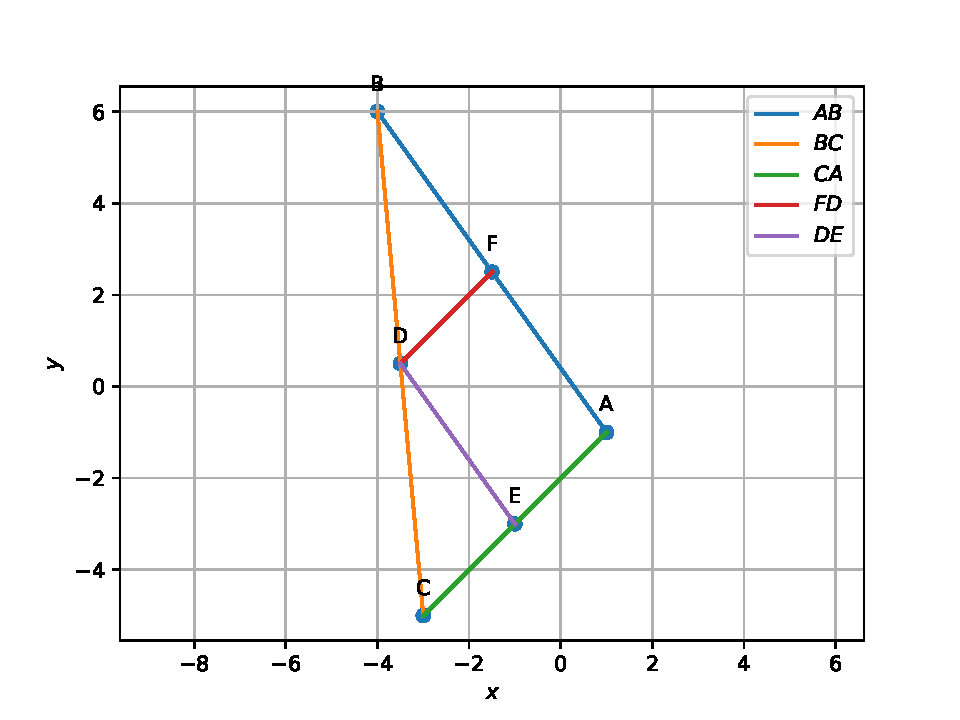
\includegraphics[width=0.75\columnwidth]{figs/triangle/pgm.pdf}
\caption{$AFDE$ forms a parallelogram in triangle ABC}
\label{fig:Triangle-pgm}
\end{figure}






















\item   Points $\vec{A}, \vec{B}, \vec{C}$ are defined to be collinear if 
		\begin{align}
			\label{eq:app-app-line-rank}
			\rank{\myvec{1 & 1 & 1 \\ \vec{A}& \vec{B}&\vec{C}}} = 2
		\end{align}
Are the given points in
			\eqref{eq:app-tri-pts}
collinear?
\\
\solution 
From 
			\eqref{eq:app-tri-pts},
\begin{align}
    \label{eq:app-1.1.3,2}
\myvec{
    1 & 1 & 1\\
    \vec{A} & \vec{B} & \vec{C} \\
    } 
    =
    %\label{eq:app-matthrowoperations}
    \myvec{
    1 & 1 & 1
    \\
    1 & -4 & -3
    \\
    -1 & 6 & -5
    }
     \xleftrightarrow[]{R_3 \leftarrow R_3+R_2}
    \myvec{
    1 & 1 & 1
    \\
    1 & -4 & -3
    \\
    0 & 2 & -8 
    }
    \\
     \xleftrightarrow[]{R_2\leftarrow R_1-R_2}
    \myvec{
    1 & 1 & 1
    \\
    0 & 5 & 4
    \\
    0 & 2 & -8 
    }
     \xleftrightarrow[]{R_3\leftarrow R_3-\frac{2}{5}R_2}
    \myvec{
    1 & 1 & 1
    \\
    0 & 5 & 4
    \\
    0 & 0 & \frac{-48}{5}
    }
\end{align}
There are no zero rows. So,
\begin{align}
    \text{rank}\myvec{
    1 & 1 & 1\\
    \vec{A} & \vec{B} & \vec{C} \\
    } &= 3 
\end{align}  
Hence,  the points $\vec{A},\vec{B},\vec{C}$ are not collinear. 
This is visible in 
\figref{fig1:Triangle}.
\begin{figure}[H]
\centering
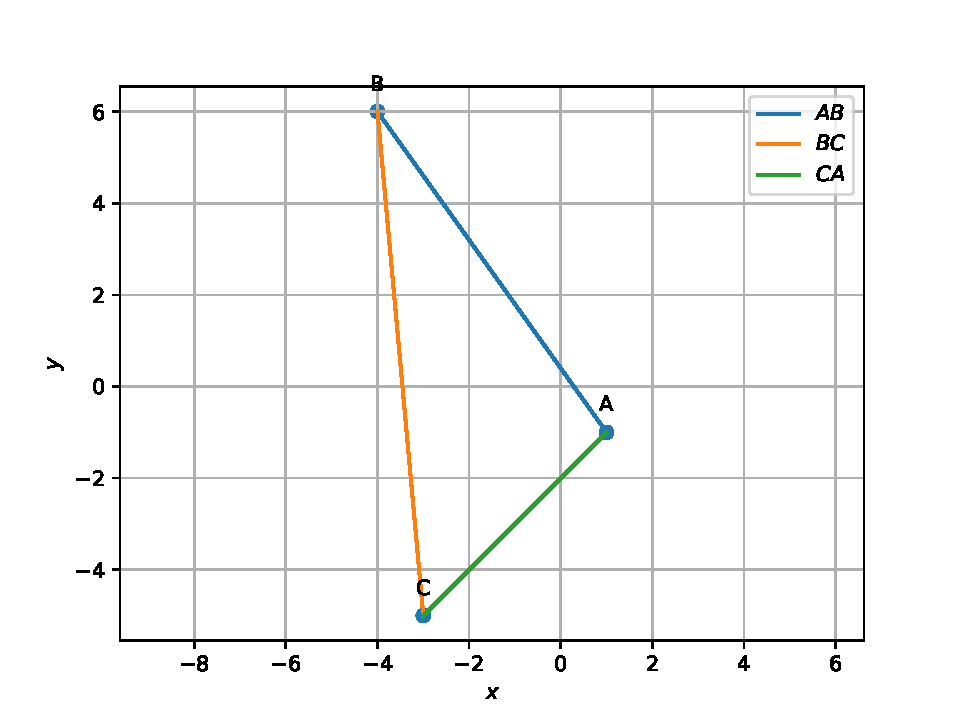
\includegraphics[width=0.75\columnwidth]{figs/triangle/vector.pdf}
\caption{$\triangle ABC$}
\label{fig1:Triangle}
\end{figure}
% \\		\\ \solution 
\begin{align}
    \vec{A}-\vec{F}&=\myvec{1\\-1}-\myvec{\frac{-3}{2}\\\frac{5}{2}}
    =\myvec{\frac{5}{2}\\\frac{-7}{2}}
    \\
    \vec{E}-\vec{D}&=\myvec{-1\\-3}-\myvec{\frac{-7}{2}\\\frac{1}{2}}
    =\myvec{\frac{5}{2}\\\frac{-7}{2}}
    \\
	\implies	\vec{A}-\vec{F} &= \vec{E}-\vec{D}
\end{align}
See \figref{fig:Triangle-pgm}, 
\begin{figure}
\centering
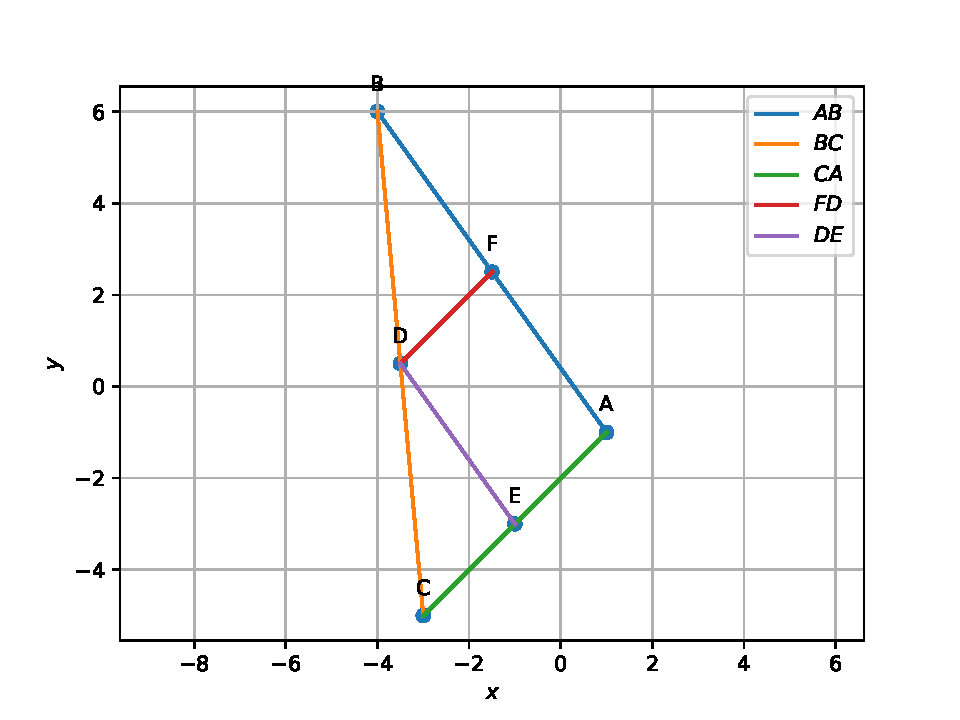
\includegraphics[width=0.75\columnwidth]{figs/triangle/pgm.pdf}
\caption{$AFDE$ forms a parallelogram in triangle ABC}
\label{fig:Triangle-pgm}
\end{figure}






















\item The parameteric form of the equation  of $AB$ is 
		\begin{align}
			\label{eq:app-geo-param}
			\vec{x}=\vec{A}+k\vec{m} \quad k \ne 0,
		\end{align}
		where
		\begin{align}
\vec{m}=\vec{B}-\vec{A}
		\end{align}
is the direction vector of $AB$.
Find the parameteric equations of $AB, BC$ and $CA$.
\\
\solution
From 
			\eqref{eq:app-geo-param} and
		\eqref{eq:app-geo-dir-vec-ab},
the parametric equation for $AB$ is given by
\begin{align}
AB: \vec{x} = &\myvec{1\\-1} + k \myvec{-5\\7}
\end{align}
Similarly, from 
		\eqref{eq:app-geo-dir-vec-bc} and
		\eqref{eq:app-geo-dir-vec-ca},
\begin{align}
BC: \vec{x} = &\myvec{-4\\6} + k \myvec{1\\-11}\\
CA: \vec{x} = &\myvec{-3\\-5} + k \myvec{4\\4}
\end{align}

%		\\ \solution 
\begin{align}
    \vec{A}-\vec{F}&=\myvec{1\\-1}-\myvec{\frac{-3}{2}\\\frac{5}{2}}
    =\myvec{\frac{5}{2}\\\frac{-7}{2}}
    \\
    \vec{E}-\vec{D}&=\myvec{-1\\-3}-\myvec{\frac{-7}{2}\\\frac{1}{2}}
    =\myvec{\frac{5}{2}\\\frac{-7}{2}}
    \\
	\implies	\vec{A}-\vec{F} &= \vec{E}-\vec{D}
\end{align}
See \figref{fig:Triangle-pgm}, 
\begin{figure}
\centering
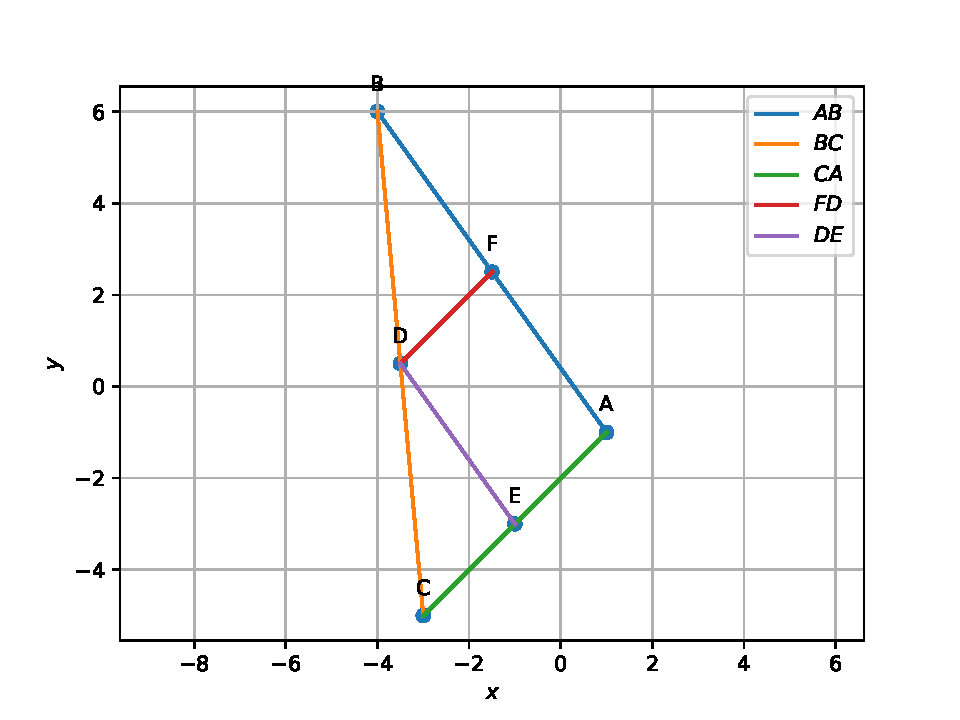
\includegraphics[width=0.75\columnwidth]{figs/triangle/pgm.pdf}
\caption{$AFDE$ forms a parallelogram in triangle ABC}
\label{fig:Triangle-pgm}
\end{figure}






















\item The normal form of the equation of $AB$  is 
		\begin{align}
			\label{eq:app-geo-normal}
			\vec{n}^{\top}\brak{	\vec{x}-\vec{A}} = 0
		\end{align}
		where 
		\begin{align}
			\vec{n}^{\top}\vec{m}&=\vec{n}^{\top}\brak{\vec{B}-\vec{A}} = 0
			\\
			\text{or, } \vec{n}&=\myvec{0 & 1 \\ -1 & 0} \vec{m}
			\label{eq:app-geo-norm-vec}
		\end{align}
Find the normal form of the equations of $AB, BC$ and $CA$.
\\
\solution
\begin{enumerate}
	\item
From
		\eqref{eq:app-geo-dir-vec-bc}, 
the direction vector of side $\vec{BC}$ is
\begin{align}
\vec{m}
	&=\myvec{1\\-11}
	\\
\implies \vec{n} &= \myvec{0 & 1\\
  -1 & 0}\myvec{1\\-11}
 = \myvec{-11\\-1}
		\label{eq:app-geo-norm-vec-bc}
\end{align}
from 
			\eqref{eq:app-geo-norm-vec}.
Hence, from 
			\eqref{eq:app-geo-normal},
the normal equation of side $BC$ is 
\begin{align}
	\vec{n}^{\top}\brak{	\vec{x}-\vec{B}} &= 0
			\\
\implies    \myvec{-11 & -1}\vec{x}&=\myvec{-11 & -1}\myvec{-4\\6}\\
    \implies
BC: \quad    \myvec{11 & 1}\vec{x}&=-38
\end{align}
\item Similarly, for $AB$,
from 
		\eqref{eq:app-geo-dir-vec-ab}, 
\begin{align}
	\vec{m} &= \myvec{-5\\7}
	\\
\implies        \vec{n} 
                &= \myvec{0&1\\-1&0}\myvec{-5\\7}
                = \myvec{7\\5}
		\label{eq:app-geo-norm-vec-ab}
\end{align}
and 
\begin{align}
	\vec{n}^{\top}\brak{	\vec{x}-\vec{A}} &= 0
	\\
	\implies
                AB: \quad  \vec{n}^{\top}\vec{x} &= \myvec{7&5}\myvec{1\\-1}\\    
       \implies\myvec{7&5}\vec{x} &= 2
\end{align}
\item For 
$CA$, 
from 
		\eqref{eq:app-geo-dir-vec-ca}, 
\begin{align}
\vec{m} &= \myvec{1 \\ 1}
\\
		\label{eq:app-geo-norm-vec-ca}
\implies \vec{n} 
&= \myvec{0&1 \\ -1&0}\myvec{1 \\ 1}
= \myvec{1 \\ -1}\\
\\
\implies	\vec{n}^{\top}\brak{	\vec{x}-\vec{C}} &= 0
\\
\implies \myvec{1&-1}{\vec{x}} &= \myvec{1&-1}\myvec{-3 \\ -5} 
= 2 
\end{align}
\end{enumerate}

%\begin{enumerate}
	\item
From
		\eqref{eq:geo-dir-vec-bc}, 
the direction vector of side $\vec{BC}$ is
\begin{align}
\vec{m}
	&=\myvec{1\\-11}
	\\
\implies \vec{n} &= \myvec{0 & 1\\
  -1 & 0}\myvec{1\\-11}
 = \myvec{-11\\-1}
		\label{eq:geo-norm-vec-bc}
\end{align}
from 
			\eqref{eq:geo-norm-vec}.
Hence, from 
			\eqref{eq:geo-normal},
the normal equation of side $BC$ is 
\begin{align}
	\vec{n}^{\top}\brak{	\vec{x}-\vec{B}} &= 0
			\\
\implies    \myvec{-11 & -1}\vec{x}&=\myvec{-11 & -1}\myvec{-4\\6}\\
    \implies
BC: \quad    \myvec{11 & 1}\vec{x}&=-38
\end{align}
\item Similarly, for $AB$,
from 
		\eqref{eq:geo-dir-vec-ab}, 
\begin{align}
	\vec{m} &= \myvec{-5\\7}
	\\
\implies        \vec{n} 
                &= \myvec{0&1\\-1&0}\myvec{-5\\7}
                = \myvec{7\\5}
		\label{eq:geo-norm-vec-ab}
\end{align}
and 
\begin{align}
	\vec{n}^{\top}\brak{	\vec{x}-\vec{A}} &= 0
	\\
	\implies
                AB: \quad  \vec{n}^{\top}\vec{x} &= \myvec{7&5}\myvec{1\\-1}\\    
       \implies\myvec{7&5}\vec{x} &= 2
\end{align}
\item For 
$CA$, 
from 
		\eqref{eq:geo-dir-vec-ca}, 
\begin{align}
\vec{m} &= \myvec{1 \\ 1}
\\
		\label{eq:geo-norm-vec-ca}
\implies \vec{n} 
&= \myvec{0&1 \\ -1&0}\myvec{1 \\ 1}
= \myvec{1 \\ -1}\\
\\
\implies	\vec{n}^{\top}\brak{	\vec{x}-\vec{C}} &= 0
\\
\implies \myvec{1&-1}{\vec{x}} &= \myvec{1&-1}\myvec{-3 \\ -5} 
= 2 
\end{align}
\end{enumerate}


\item The area of $\triangle ABC$ is defined as
		\begin{align}
			\label{eq:app-tri-area-cross}
			\frac{1}{2}\norm{{\brak{\vec{A}-\vec{B}}\times \brak{\vec{A}-\vec{C}}}}
		\end{align}
		where
		\begin{align}
			\vec{A}\times\vec{B} \triangleq \mydet{1 & -4 \\-1 & 6}
		\end{align}
		Find the area of $\triangle ABC$.\\
\solution
From
		\eqref{eq:app-geo-dir-vec-ab}
		and
		\eqref{eq:app-geo-dir-vec-ca},
\begin{align}
	\vec{A}-\vec{B}=\myvec{5\\-7},
	\vec{A}-\vec{C}&=\myvec{4\\4}\\
\implies (\vec{A}-\vec{B})\times(\vec{A}-\vec{C}) &=\mydet{5 & 4\\-7 & 4}\\
&=5\times 4-4\times (-7)\\&=48\\
\implies\frac{1}{2}\norm{(\vec{A}-\vec{B})\times(\vec{A}-\vec{C})}&=\frac{48}{2}=24
\end{align}
which is the desired area.

%  		\\ \solution 
\begin{align}
    \vec{A}-\vec{F}&=\myvec{1\\-1}-\myvec{\frac{-3}{2}\\\frac{5}{2}}
    =\myvec{\frac{5}{2}\\\frac{-7}{2}}
    \\
    \vec{E}-\vec{D}&=\myvec{-1\\-3}-\myvec{\frac{-7}{2}\\\frac{1}{2}}
    =\myvec{\frac{5}{2}\\\frac{-7}{2}}
    \\
	\implies	\vec{A}-\vec{F} &= \vec{E}-\vec{D}
\end{align}
See \figref{fig:Triangle-pgm}, 
\begin{figure}
\centering
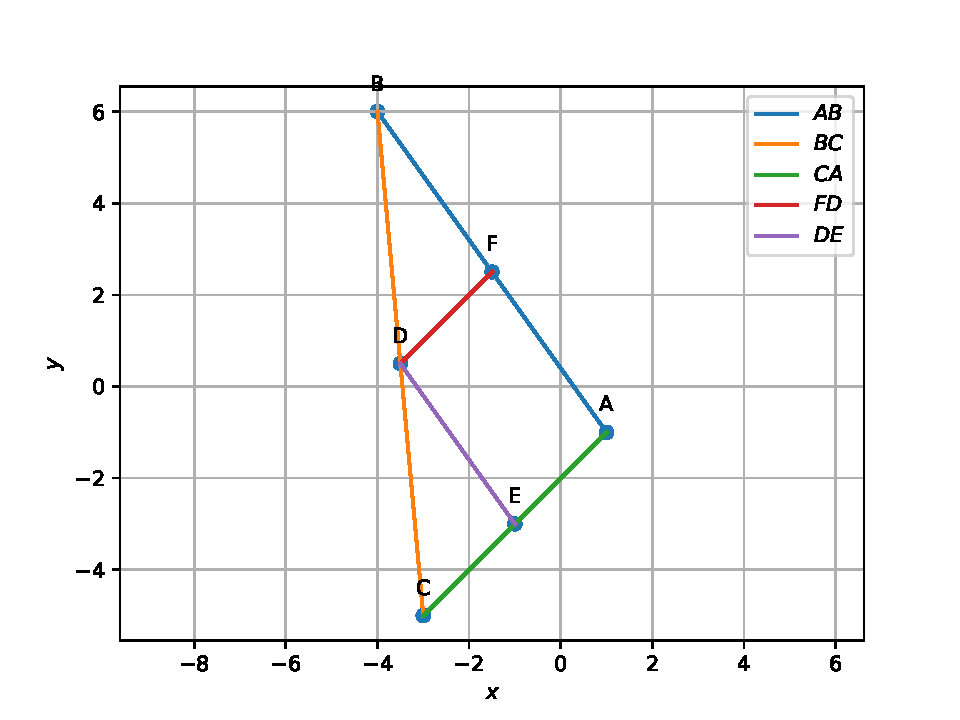
\includegraphics[width=0.75\columnwidth]{figs/triangle/pgm.pdf}
\caption{$AFDE$ forms a parallelogram in triangle ABC}
\label{fig:Triangle-pgm}
\end{figure}






















	\item Find the angles $A, B, C$ if 
%    \label{prop:angle2d}
  \begin{align}
    \label{eq:app-angle2d}
			\cos A \triangleq 
\frac{\brak{\vec{B}-\vec{A}}^{\top}{\vec{C}-\vec{A}}}{\norm{\vec{B}-\vec{A}}\norm{\vec{C}-\vec{A}}}
  \end{align}\\
  \solution
\begin{enumerate}
	\item From 
		\eqref{eq:app-geo-dir-vec-ab},
		\eqref{eq:app-geo-dir-vec-ca},
		\eqref{eq:app-geo-norm-ab}
		and
		\eqref{eq:app-geo-norm-ca}
\begin{align}
	(\vec{B}-\vec{A})^{\top}(\vec{C}-\vec{A})&=\myvec{-5&7}\myvec{-4\\-4}\\
	&=-8
	\\
	\implies
	\cos{A}&= \frac{-8}{\sqrt{74} \sqrt{32}}
	= \frac{-1}{\sqrt{37}}\\
	\implies A&=\cos^{-1}{\frac{-1}{\sqrt{37}}}
\end{align}
	\item From 
		\eqref{eq:app-geo-dir-vec-ab},
		\eqref{eq:app-geo-dir-vec-bc},
		\eqref{eq:app-geo-norm-ab}
		and
		\eqref{eq:app-geo-norm-bc}
\begin{align}
	(\vec{C}-\vec{B})^{\top}(\vec{A}-\vec{B})&=\myvec{1&-11}\myvec{5\\-7}\\
	&= 82
	\\
	\implies
	\cos{B}&= \frac{82}{\sqrt{74} \sqrt{122}}
	= \frac{41}{\sqrt{2257}}\\
	\implies B&=\cos^{-1}{\frac{41}{\sqrt{2257}}}
\end{align}
	\item From 
		\eqref{eq:app-geo-dir-vec-bc},
		\eqref{eq:app-geo-dir-vec-ca},
		\eqref{eq:app-geo-norm-bc}
		and
		\eqref{eq:app-geo-norm-ca}
\begin{align}
	(\vec{A}-\vec{C})^{\top}(\vec{B}-\vec{C})&=\myvec{4&4}\myvec{-1\\11}\\
	&=40
	\\
\implies	\cos{C}&= \frac{40}{\sqrt{32} \sqrt{122}}
	= \frac{5}{\sqrt{61}}\\
	\implies C&=\cos^{-1}{\frac{5}{\sqrt{61}}}
\end{align}

\end{enumerate}
%  	\\ \solution 
\begin{align}
    \vec{A}-\vec{F}&=\myvec{1\\-1}-\myvec{\frac{-3}{2}\\\frac{5}{2}}
    =\myvec{\frac{5}{2}\\\frac{-7}{2}}
    \\
    \vec{E}-\vec{D}&=\myvec{-1\\-3}-\myvec{\frac{-7}{2}\\\frac{1}{2}}
    =\myvec{\frac{5}{2}\\\frac{-7}{2}}
    \\
	\implies	\vec{A}-\vec{F} &= \vec{E}-\vec{D}
\end{align}
See \figref{fig:Triangle-pgm}, 
\begin{figure}
\centering
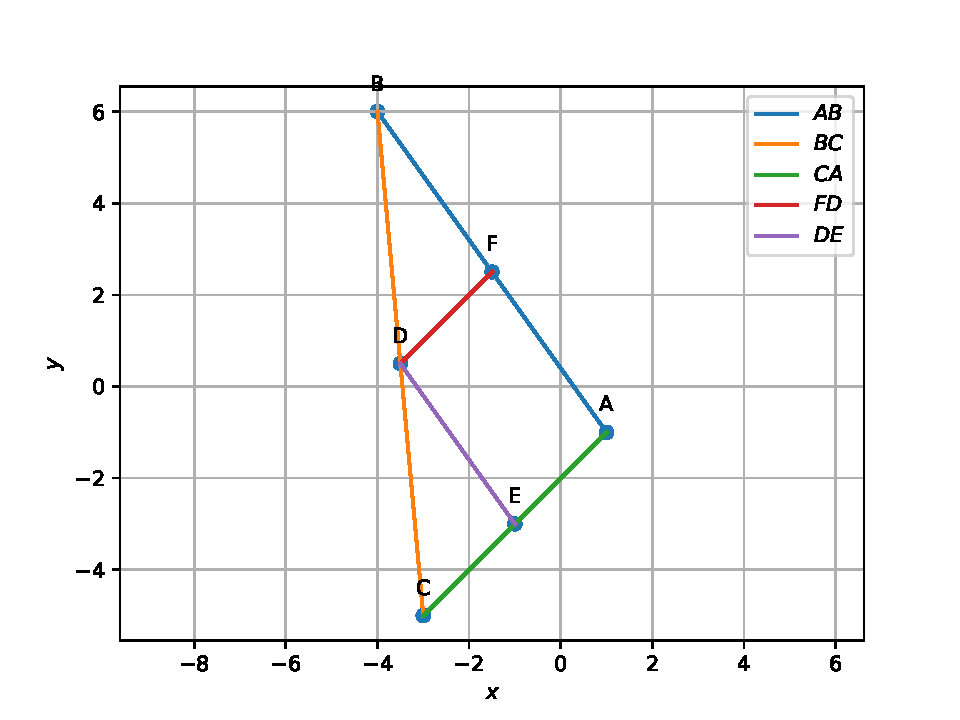
\includegraphics[width=0.75\columnwidth]{figs/triangle/pgm.pdf}
\caption{$AFDE$ forms a parallelogram in triangle ABC}
\label{fig:Triangle-pgm}
\end{figure}






















All codes for this section are available at
\begin{lstlisting}
	codes/triangle/sides.py
\end{lstlisting}
\end{enumerate}

\item If the points $\vec{A}(6,  1),  \vec{B}(8,  2),  \vec{C}(9,  4)$ and $\vec{D}(p,  3)$ are the vertices of a parallelogram,  taken in order,  find the value of $p$.
\label{10/7/0/10}
\item 
If $(1,  2),  (4,  y),  (x,  6)$ and $(3,  5)$ are the vertices of a parallelogram taken in order,  find $x$ and $y$.
\label{10/7/2/6}
\item The fourth vertex $\vec{D}$ of a parallelogram $ABCD$ whose three vertices are
	$\vec{A} (–2,  3),  \vec{B} (6,  7)$ and  $\vec{C} (8,  3)$ is
\item Verify if the points $\vec{A}(4, 3),  \vec{B}(6, 4), \vec{C}(5, -6)$  and  $\vec{D}(-3, 5)$ are the vertices of a parallelogram.
\item A girl walks 4 km towards west,  then she walks 3 km in a direction 30$^{\circ}$ east of north and stops. Determine the girl's displacement from her initial point of departure.\\
	\solution
		\iffalse
\documentclass[10pt]{article}
\usepackage{graphicx}
\def\inputGnumericTable{}
\usepackage[latin1]{inputenc}
\usepackage{fullpage}
\usepackage{color}
\usepackage{array}
\usepackage{longtable}
\usepackage{calc}
\usepackage{multirow}
\usepackage{hhline}
\usepackage{ifthen}
\usepackage{amsmath}
\usepackage[none]{hyphenat}
\usepackage{listings}
\usepackage[english]{babel}
\usepackage{siunitx}
\usepackage{caption}
\usepackage{booktabs}
\usepackage{array}
\usepackage{extarrows}
\usepackage{enumerate}
\usepackage{enumitem}
\usepackage{amsmath}
\usepackage{commath}
\usepackage{gensymb}
\usepackage{amssymb}
\usepackage{multicol}
%\usepackage[utf8]{inputenc}
\lstset{
 frame=single,
 breaklines=true
}
\usepackage{hyperref}
\usepackage[margin=0.65in]{geometry}	 
%\usepackage{exsheets}% also loads the `tasks' package
\usepackage{atbegshi}
\AtBeginDocument{\AtBeginShipoutNext{\AtBeginShipoutDiscard}}

%new macro definitions
\renewcommand{\labelenumi}{(\roman{enumi})}
\newcommand{\mydet}[1]{\ensuremath{\begin{vmatrix}#1\end{vmatrix}}}
\providecommand{\brak}[1]{\ensuremath{\left(#1\right)}}
\newcommand{\solution}{\noindent \textbf{Solution: }}
\newcommand{\myvec}[1]{\ensuremath{\begin{pmatrix}#1\end{pmatrix}}}
\newenvironment{amatrix}[1]{%
	\left(\begin{array}{@{}*{#1}{c}|c@{}}
}{%
	\end{array}\right)
}

\newcommand{\myaugvec}[2]{\ensuremath{\begin{amatrix}{#1}#2\end{amatrix}}}
\providecommand{\norm}[1]{\left\1Vert#1\right\rVert}
\let\vec\mathbf{}


%\SetEnumitemKey{twocol}{
% before=\raggedcolumns\begin{multicols}{2},
% after=\end{multicols}}
%\SetEnumitemKey{fourcol}{
% before=\raggedcolumns\begin{multicols}{4},
% after=\end{multicols}} 


\begin{document}
\begin{center}
\title{\textbf{TRIANGLES}}
\date{\vspace{-5ex}}
\maketitle
\end{center}
\section*{9$^{th}$Math - Chapter 7}
This is Problem-8 from Exercise 7.1\\\\


\section*{\large Construction:}
\fi
The input parameters for construction
	are available in Table \ref{tab:chapters/9/7/1/8/table}.
\begin{table}[H]
	\centering
	%\subimport{../chapters/9/7/1/8/tables/}{table.tex}
     %%%%%%%%%%%%%%%%%%%%%%%%%%%%%%%%%%%%%%%%%%%%%%%%%%%%%%%%%%%%%%%%%%%%%%
%%                                                                  %%
%%  This is the header of a LaTeX2e file exported from Gnumeric.    %%
%%                                                                  %%
%%  This file can be compiled as it stands or included in another   %%
%%  LaTeX document. The table is based on the longtable package so  %%
%%  the longtable options (headers, footers...) can be set in the   %%
%%  preamble section below (see PRAMBLE).                           %%
%%                                                                  %%
%%  To include the file in another, the following two lines must be %%
%%  in the including file:                                          %%
%%        \def\inputGnumericTable{}                                 %%
%%  at the beginning of the file and:                               %%
%%        \input{name-of-this-file.tex}                             %%
%%  where the table is to be placed. Note also that the including   %%
%%  file must use the following packages for the table to be        %%
%%  rendered correctly:                                             %%
%%    \usepackage[latin1]{inputenc}                                 %%
%%    \usepackage{color}                                            %%
%%    \usepackage{array}                                            %%
%%    \usepackage{longtable}                                        %%
%%    \usepackage{calc}                                             %%
%%    \usepackage{multirow}                                         %%
%%    \usepackage{hhline}                                           %%
%%    \usepackage{ifthen}                                           %%
%%  optionally (for landscape tables embedded in another document): %%
%%    \usepackage{lscape}                                           %%
%%                                                                  %%
%%%%%%%%%%%%%%%%%%%%%%%%%%%%%%%%%%%%%%%%%%%%%%%%%%%%%%%%%%%%%%%%%%%%%



%%  This section checks if we are begin input into another file or  %%
%%  the file will be compiled alone. First use a macro taken from   %%
%%  the TeXbook ex 7.7 (suggestion of Han-Wen Nienhuys).            %%
\def\ifundefined#1{\expandafter\ifx\csname#1\endcsname\relax}


%%  Check for the \def token for inputed files. If it is not        %%
%%  defined, the file will be processed as a standalone and the     %%
%%  preamble will be used.                                          %%
\ifundefined{inputGnumericTable}

%%  We must be able to close or not the document at the end.        %%
	\def\gnumericTableEnd{\end{document}}


%%%%%%%%%%%%%%%%%%%%%%%%%%%%%%%%%%%%%%%%%%%%%%%%%%%%%%%%%%%%%%%%%%%%%%
%%                                                                  %%
%%  This is the PREAMBLE. Change these values to get the right      %%
%%  paper size and other niceties.                                  %%
%%                                                                  %%
%%%%%%%%%%%%%%%%%%%%%%%%%%%%%%%%%%%%%%%%%%%%%%%%%%%%%%%%%%%%%%%%%%%%%%

	\documentclass[12pt%
			  %,landscape%
                    ]{report}
       \usepackage[latin1]{inputenc}
       \usepackage{fullpage}
       \usepackage{color}
       \usepackage{array}
       \usepackage{longtable}
       \usepackage{calc}
       \usepackage{multirow}
       \usepackage{hhline}
       \usepackage{ifthen}
       \usepackage{gensymb}
       \usepackage{graphicx}
\usepackage{amsmath}
\usepackage{mathtools}
\newcommand{\mydet}[1]{\ensuremath{\begin{vmatrix}#1\end{vmatrix}}}
\providecommand{\brak}[1]{\ensuremath{\left(#1\right)}}
\providecommand{\norm}[1]{\left\lVert#1\right\rVert}
\newcommand{\solution}{\noindent \textbf{Solution: }}
\newcommand{\myvec}[1]{\ensuremath{\begin{pmatrix}#1\end{pmatrix}}}
\let\vec\mathbf
	\begin{document}


%%  End of the preamble for the standalone. The next section is for %%
%%  documents which are included into other LaTeX2e files.          %%
\else

%%  We are not a stand alone document. For a regular able, we will %%
%%  have no preamble and only define the closing to mean nothing.   %%
    \def\gnumericTableEnd{}

%%  If we want landscape mode in an embedded document, comment out  %%
%%  the line above and uncomment the two below. The table will      %%
%%  begin on a new page and run in landscape mode.                  %%
%       \def\gnumericTableEnd{\end{landscape}}
%       \begin{landscape}


%%  End of the else clause for this file being \input.              %%
\fi

%%%%%%%%%%%%%%%%%%%%%%%%%%%%%%%%%%%%%%%%%%%%%%%%%%%%%%%%%%%%%%%%%%%%%%
%%                                                                  %%
%%  The rest is the gnumeric table, except for the closing          %%
%%  statement. Changes below will alter the table's appearance.     %%
%%                                                                  %%
%%%%%%%%%%%%%%%%%%%%%%%%%%%%%%%%%%%%%%%%%%%%%%%%%%%%%%%%%%%%%%%%%%%%%%
\providecommand{\gnumericmathit}[1]{#1} 
%%  Uncomment the next line if you would like your numbers to be in %%
%%  italics if they are italizised in the gnumeric table.           %%
%\renewcommand{\gnumericmathit}[1]{\mathit{#1}}
\providecommand{\gnumericPB}[1]%
{\let\gnumericTemp=\\#1\let\\=\gnumericTemp\hspace{0pt}}
 \ifundefined{gnumericTableWidthDefined}
        \newlength{\gnumericTableWidth}
        \newlength{\gnumericTableWidthComplete}
        \newlength{\gnumericMultiRowLength}
        \global\def\gnumericTableWidthDefined{}
 \fi
%% The following setting protects this code from babel shorthands.  %%
 \ifthenelse{\isundefined{\languageshorthands}}{}{\languageshorthands{english}}
%%  The default table format retains the relative column widths of  %%
%%  gnumeric. They can easily be changed to c, r or l. In that case %%
%%  you may want to comment out the next line and uncomment the one %%
%%  thereafter                                                      %%
\providecommand\gnumbox{\makebox[0pt]}
%%\providecommand\gnumbox[1][]{\makebox}

%% to adjust positions in multirow situations                       %%
\setlength{\bigstrutjot}{\jot}
\setlength{\extrarowheight}{\doublerulesep}

%%  The \setlongtables command keeps column widths the same across  %%
%%  pages. Simply comment out next line for varying column widths.  %%
\setlongtables

\setlength\gnumericTableWidth{%
	40pt+%
	35pt+%
	210pt+%
0pt}
\def\gumericNumCols{3}
\setlength\gnumericTableWidthComplete{\gnumericTableWidth+%
         \tabcolsep*\gumericNumCols*2+\arrayrulewidth*\gumericNumCols}
\ifthenelse{\lengthtest{\gnumericTableWidthComplete > \linewidth}}%
         {\def\gnumericScale{\ratio{\linewidth-%
                        \tabcolsep*\gumericNumCols*2-%
                        \arrayrulewidth*\gumericNumCols}%
{\gnumericTableWidth}}}%
{\def\gnumericScale{1}}

%%%%%%%%%%%%%%%%%%%%%%%%%%%%%%%%%%%%%%%%%%%%%%%%%%%%%%%%%%%%%%%%%%%%%%
%%                                                                  %%
%% The following are the widths of the various columns. We are      %%
%% defining them here because then they are easier to change.       %%
%% Depending on the cell formats we may use them more than once.    %%
%%                                                                  %%
%%%%%%%%%%%%%%%%%%%%%%%%%%%%%%%%%%%%%%%%%%%%%%%%%%%%%%%%%%%%%%%%%%%%%%

\ifthenelse{\isundefined{\gnumericColA}}{\newlength{\gnumericColA}}{}\settowidth{\gnumericColA}{\begin{tabular}{@{}p{40pt*\gnumericScale}@{}}x\end{tabular}}
\ifthenelse{\isundefined{\gnumericColB}}{\newlength{\gnumericColB}}{}\settowidth{\gnumericColB}{\begin{tabular}{@{}p{35pt*\gnumericScale}@{}}x\end{tabular}}
\ifthenelse{\isundefined{\gnumericColC}}{\newlength{\gnumericColC}}{}\settowidth{\gnumericColC}{\begin{tabular}{@{}p{65pt*\gnumericScale}@{}}x\end{tabular}}

\begin{longtable}[c]{%
	b{\gnumericColA}%
	b{\gnumericColB}%
	b{\gnumericColC}%
	}

%%%%%%%%%%%%%%%%%%%%%%%%%%%%%%%%%%%%%%%%%%%%%%%%%%%%%%%%%%%%%%%%%%%%%%
%%  The longtable options. (Caption, headers... see Goosens, p.124) %%
%	\caption{The Table Caption.}             \\	%
% \hline	% Across the top of the table.
%%  The rest of these options are table rows which are placed on    %%
%%  the first, last or every page. Use \multicolumn if you want.    %%

%%  Header for the first page.                                      %%
%	\multicolumn{3}{c}{The First Header} \\ \hline 
%	\multicolumn{1}{c}{colTag}	%Column 1
%	&\multicolumn{1}{c}{colTag}	%Column 2
%	&\multicolumn{1}{c}{colTag}	\\ \hline %Last column
%	\endfirsthead

%%  The running header definition.                                  %%
%	\hline
%	\multicolumn{3}{l}{\ldots\small\slshape continued} \\ \hline
%	\multicolumn{1}{c}{colTag}	%Column 1
%	&\multicolumn{1}{c}{colTag}	%Column 2
%	&\multicolumn{1}{c}{colTag}	\\ \hline %Last column
%	\endhead

%%  The running footer definition.                                  %%
%	\hline
%	\multicolumn{3}{r}{\small\slshape continued\ldots} \\
%	\endfoot

%%  The ending footer definition.                                   %%
%	\multicolumn{3}{c}{That's all folks} \\ \hline 
%	\endlastfoot
%%%%%%%%%%%%%%%%%%%%%%%%%%%%%%%%%%%%%%%%%%%%%%%%%%%%%%%%%%%%%%%%%%%%%%

\hhline{|-|-|-}
	 \multicolumn{1}{|p{\gnumericColA}|}%
	{\gnumericPB{\raggedright}\gnumbox[l]{\textbf{Symbol}}}
	&\multicolumn{1}{p{\gnumericColB}|}%
	{\gnumericPB{\raggedright}\gnumbox[l]{\textbf{Values}}}
	&\multicolumn{1}{p{\gnumericColC}|}%
	{\gnumericPB{\raggedright}\gnumbox[l]{\textbf{Description}}}
\\
\hhline{|---|}
	 \multicolumn{1}{|p{\gnumericColA}|}%
	{\gnumericPB{\raggedright}\gnumbox[l]{$r$}}
	&\multicolumn{1}{p{\gnumericColB}|}%
	{\gnumericPB{\raggedright}\gnumbox[l]{2}}
	&\multicolumn{1}{p{\gnumericColC}|}%
	{\gnumericPB{\raggedright}\gnumbox[l]{radius}}
\\
\hhline{|---|}
	 \multicolumn{1}{|p{\gnumericColA}|}%
	{\gnumericPB{\raggedright}\gnumbox[l]{$\vec{O}$}}
	&\multicolumn{1}{p{\gnumericColB}|}%
	{\gnumericPB{\raggedright}\gnumbox[l]{$\myvec{0\\0}$}}
	&\multicolumn{1}{p{\gnumericColC}|}%
	{\gnumericPB{\raggedright}\gnumbox[l]{center}}
\\
\hhline{|---|}
\end{longtable}

\ifthenelse{\isundefined{\languageshorthands}}{}{\languageshorthands{\languagename}}
\gnumericTableEnd%t

	\caption{}
	\label{tab:chapters/9/7/1/8/table}
\end{table}
Thus, 
\begin{align}
	\vec{A}=\myvec{0\\b},\,
	\vec{B}=\myvec{a\\0},\,
	\vec{C}=\myvec{0\\0}
\end{align}
yielding
\begin{align}
	\vec{M}&=\frac{\vec{A}+\vec{B}}{2}=\frac{1}{2}\myvec{a\\b}
\end{align}
Also, 
\begin{align}
	\vec{M}&=\frac{\vec{C}+\vec{D}}{2}\\
	\implies \vec{D}&=2\vec{M}-\vec{C}=\myvec{a\\b}
\end{align}
\iffalse
\solution
Given
\begin{align}
	\vec{M}&=\frac{\vec{A}+\vec{B}}{2}
	\label{eq:chapters/9/7/1/8/1}\\
	\vec{D}-\vec{M}&=\vec{C}-\vec{M}
	\label{eq:chapters/9/7/1/8/2}\\
	\angle ACB&=90\degree
\end{align}
\textbf{Proof:} From Figure \ref{fig:chapters/9/7/1/8/1}
\fi
Thus,
\begin{align}
	\brak{\vec{D}-\vec{B}}^{\top}\brak{\vec{B}-\vec{C}} &= \myvec{0 & b}\myvec{a\\0}=0\\
	\implies BD & \perp BC\\
\end{align}
Also, 
\begin{align}
	\norm{\vec{A}-\vec{B}}&=\norm{\myvec{-a\\b}}\\
	\norm{\vec{C}-\vec{D}}&=\norm{\myvec{-a\\-b}}\\
	\implies \norm{\vec{A}-\vec{B}} &= \norm{\vec{C}-\vec{D}}\\
	\text{ or, } AB &= CD
	\label{eq:chapters/9/7/1/8/3}	
\end{align}
From \eqref{eq:chapters/9/7/1/8/3}
\begin{align}
	\implies CM = \frac{1}{2}CD = \frac{1}{2}AB 
\end{align}
See Fig. 
\ref{fig:chapters/9/7/1/8/1}.
\begin{figure}[H]
	\begin{center}
		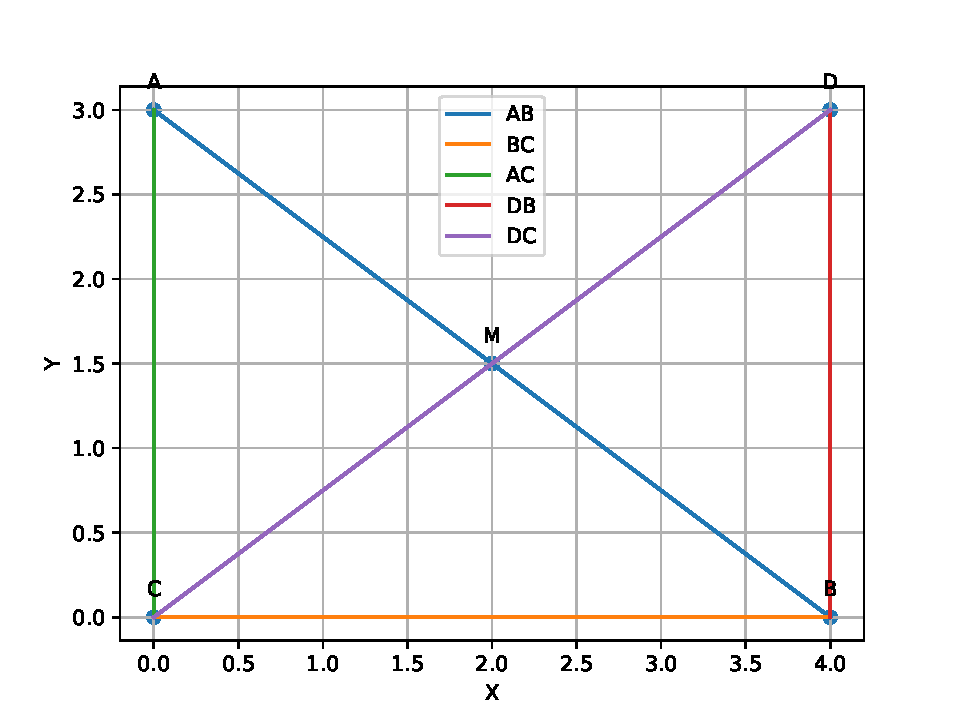
\includegraphics[width=0.75\columnwidth]{./chapters/9/7/1/8/figs/fig.pdf}
	\end{center}
\caption{}
\label{fig:chapters/9/7/1/8/1}
\end{figure}


\item $(-1, 2, 1),  (1, -2, 5),  (4, -7, 8)$ and $(2, -3, 4)$ are the vertices of a parallelogram.
\item Three vertices of a parallelogram $ABCD$ are $\vec{A}(3, -1, 2),  \vec{B}(1, -2, 4)$ and $\vec{C}(-1, 1, 2)$. Find the coordinates of the fourth vertex.
\item If the origin is the centroid of the triangle $PQR$ with vertices $\vec{P}(2a, 2, 6),  \vec{Q}(-4, 3b, -10)$ and $R(8, 14, 2c)$,  then find the values of $a,  b$ and $c$.
\item Find the slope of lines
\begin{enumerate}
\item  Passing through the points $(3, -2)$ and $(-1, 4)$
\item  Passing through the points $(3, -2)$ and $(7, -2)$
\item  passing through the points $(3, -2)$ and $(3, 4)$	
\item  Making inclination of $60\degree$ with the positive direction of x-axis.
\end{enumerate}
\item The centroid of a triangle $ABC$ is at the point $(1, 1, 1)$. If the coordinates of $\vec{A}$ and $\vec{B}$ are $(3, -5, 7)$ and $(-1, 7, -6)$,  respectively find the coordinates of the point $\vec{C}$.
\item Represent graphically a displacement of $40$ km,  $30\degree$ west of south.
	\item Rain is falling vertically with a speed of 35 $m s^{-1}$
. Winds starts blowing after sometime with a speed of 12 $m s^{-1}$ in
east to west direction. In which direction should a boy waiting at a bus stop hold his umbrella ?
%
\item A motorboat is racing towards north at 25 km/h and the water current in that region is 10 km/h in the direction of 60$\degree$ east of south. Find the resultant velocity of the boat.
\item Rain is falling vertically with a speed of 35 $m s^{-1}$
. A woman rides a bicycle with a speed of 12 $ms^{-1}$ in east to west
direction. What is the direction in which she should hold her umbrella ?
\item Rain is falling vertically with a speed of 30 $m s^{-1}$. A woman rides a bicycle with a speed  of 10 $m s^{-1}$ in the north to south direction. What is the direction in which she should
hold her umbrella?
\item A man can swim with a speed of 4.0 km/h in still water. How long does he take to cross a river 1.0 km wide if the river flows steadily at 3.0 km/h and he makes his strokes normal to the river current? How far down the river does he go when he reaches the other bank ?
\item In a harbour,  wind is blowing at the speed of 72 km/h and the flag on the mast of a boat anchored in the harbour flutters along the N-E direction. If the boat starts moving at a speed of 51 km/h to the north,  what is the direction of the flag on the mast of the boat ?
\item In which quadrant or on which axis do each of the points (-2, 4), (3, -1), (-1, 0), (1, 2) and (-3, -5) lie? Verify your answer by locating them on the Cartesian plane.
\item Plot the points $(x, y)$ given in 
\tabref{table:Table of values}.
\begin{table}[H]
	\centering
\begin{tabular}{|c|c|c|c|c|c|}
\hline	
x & -2 & -1 & 0 & 1 & 3\\
\hline
y & 8 & 7 & -1.25 & 3 & -1\\
\hline
\end{tabular}
\caption{}
\label{table:Table of values}
\end{table}
\end{enumerate}

\subsection{Section Formula}
The desired vector is
\begin{align}
\frac{1}{2}\myvec{2\\3\\4} +  \frac{1}{2}\myvec{4\\1\\-2} =\myvec{3\\2\\1} 
\end{align}




\subsection{CBSE}
The desired vector is
\begin{align}
\frac{1}{2}\myvec{2\\3\\4} +  \frac{1}{2}\myvec{4\\1\\-2} =\myvec{3\\2\\1} 
\end{align}




\subsection{Rank}
\iffalse
\documentclass[12pt]{article}
\usepackage{graphicx}
\usepackage{amsmath}
\usepackage{mathtools}
\usepackage{gensymb}

\newcommand{\mydet}[1]{\ensuremath{\begin{vmatrix}#1\end{vmatrix}}}
\providecommand{\brak}[1]{\ensuremath{\left(#1\right)}}
\providecommand{\norm}[1]{\left\lVert#1\right\rVert}
\newcommand{\solution}{\noindent \textbf{Solution: }}
\newcommand{\myvec}[1]{\ensuremath{\begin{pmatrix}#1\end{pmatrix}}}
\let\vec\mathbf

\begin{document}
\begin{center}
\textbf\large{CHAPTER-7 \\ COORDINATE GEOMETRY}
\end{center}
\section*{Excercise 7.4}

Q2. Find a relation between x and y if the points $\vec(x, y), \vec(1, 2) \text{ and } \vec(7, 0)$ are collinear.
\\
\solution
\\
The coordinates are given as
\fi
Let
	\begin{align}
	\vec{A} = \myvec{
		x\\
		y\\
		},
	\vec{B} = \myvec{
		1\\
		2\\
		},
	\vec{C} = \myvec{
		7\\
		0\\
		}
	\end{align}
	Then
	\begin{align}
\vec{D} &=\brak{\vec{A}-\vec{B}} = \brak{\myvec{x \\y } - \myvec{1 \\2 } } = \myvec{x-1 \\ y-2 }\\
\vec{E} &= \brak{\vec{A}-\vec{C}} = \brak{\myvec{x \\ y } - \myvec{7 \\0} } = \myvec{x-7 \\y}
\end{align}
Forming the collinearity matrix
\begin{align}
	\vec{F} &={\myvec{\vec{D}^{\top}\\ \vec{E}^{\top}}}
\end{align}
and performing row reduction,
\begin{align}
\label{eq:chapters/10/7/4/2chem_balance_mat_row}
\myvec{
x-1 & y-2
\\
x-7 & y
}
\xleftrightarrow[]{R_2 = R_2-R_1}
\myvec{
  x-1 & y-2
  \\
	  -6 & 2                 
	  }
	  \\
	\xleftrightarrow[]{R_2 = \frac{R_2}{-6}(x-1)-R_1}
\myvec{
x-1 & y-2
\\
	0 & -\frac{1}{3}(x-1)-(y-2)
}
\end{align}
For the rank of the matrix to be 1,
\begin{align}
	-\frac{1}{3}(x-1)-(y-2)&=0\\
	\implies \myvec{1 & 3}\vec{x} &=7	
\end{align}
For $x=-2, y=3$, see Fig. \ref{fig:chapters/10/7/4/2Fig} verifying that the points are collinear.
\begin{figure}[H]
	\begin{center} 
	    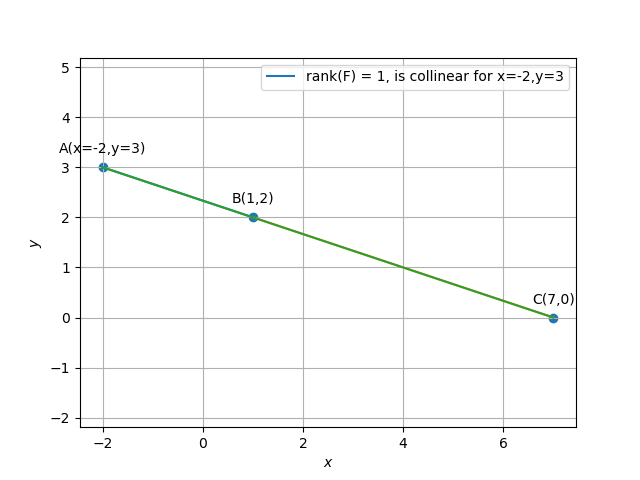
\includegraphics[width=0.75\columnwidth]{chapters/10/7/4/2/figs/sc1.png}
	\end{center}
\caption{}
\label{fig:chapters/10/7/4/2Fig}
\end{figure}

\subsection{CBSE}
\iffalse
\documentclass[12pt]{article}
\usepackage{graphicx}
\usepackage{amsmath}
\usepackage{mathtools}
\usepackage{gensymb}

\newcommand{\mydet}[1]{\ensuremath{\begin{vmatrix}#1\end{vmatrix}}}
\providecommand{\brak}[1]{\ensuremath{\left(#1\right)}}
\providecommand{\norm}[1]{\left\lVert#1\right\rVert}
\newcommand{\solution}{\noindent \textbf{Solution: }}
\newcommand{\myvec}[1]{\ensuremath{\begin{pmatrix}#1\end{pmatrix}}}
\let\vec\mathbf

\begin{document}
\begin{center}
\textbf\large{CHAPTER-7 \\ COORDINATE GEOMETRY}
\end{center}
\section*{Excercise 7.4}

Q2. Find a relation between x and y if the points $\vec(x, y), \vec(1, 2) \text{ and } \vec(7, 0)$ are collinear.
\\
\solution
\\
The coordinates are given as
\fi
Let
	\begin{align}
	\vec{A} = \myvec{
		x\\
		y\\
		},
	\vec{B} = \myvec{
		1\\
		2\\
		},
	\vec{C} = \myvec{
		7\\
		0\\
		}
	\end{align}
	Then
	\begin{align}
\vec{D} &=\brak{\vec{A}-\vec{B}} = \brak{\myvec{x \\y } - \myvec{1 \\2 } } = \myvec{x-1 \\ y-2 }\\
\vec{E} &= \brak{\vec{A}-\vec{C}} = \brak{\myvec{x \\ y } - \myvec{7 \\0} } = \myvec{x-7 \\y}
\end{align}
Forming the collinearity matrix
\begin{align}
	\vec{F} &={\myvec{\vec{D}^{\top}\\ \vec{E}^{\top}}}
\end{align}
and performing row reduction,
\begin{align}
\label{eq:chapters/10/7/4/2chem_balance_mat_row}
\myvec{
x-1 & y-2
\\
x-7 & y
}
\xleftrightarrow[]{R_2 = R_2-R_1}
\myvec{
  x-1 & y-2
  \\
	  -6 & 2                 
	  }
	  \\
	\xleftrightarrow[]{R_2 = \frac{R_2}{-6}(x-1)-R_1}
\myvec{
x-1 & y-2
\\
	0 & -\frac{1}{3}(x-1)-(y-2)
}
\end{align}
For the rank of the matrix to be 1,
\begin{align}
	-\frac{1}{3}(x-1)-(y-2)&=0\\
	\implies \myvec{1 & 3}\vec{x} &=7	
\end{align}
For $x=-2, y=3$, see Fig. \ref{fig:chapters/10/7/4/2Fig} verifying that the points are collinear.
\begin{figure}[H]
	\begin{center} 
	    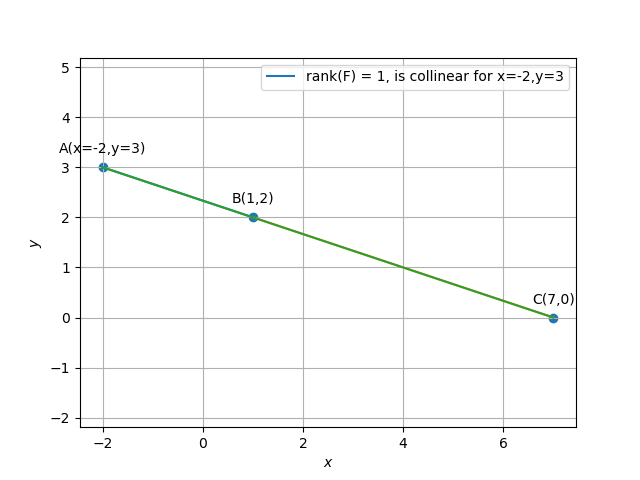
\includegraphics[width=0.75\columnwidth]{chapters/10/7/4/2/figs/sc1.png}
	\end{center}
\caption{}
\label{fig:chapters/10/7/4/2Fig}
\end{figure}

\subsection{Length}
\begin{enumerate}[label=\thesubsection.\arabic*, ref=\thesubsection.\theenumi]
\item Compute the magnitude of the following vectors:
\begin{align}
	\vec{a}&=\hat{i}+\hat{j}+\hat{k}
	\\
	\vec{b}&=2\hat{i}-7\hat{j}-3\hat{k}
	\\
	\vec{c}&=\frac{1}{\sqrt{3}}\hat{i}+\frac{1}{\sqrt{3}}\hat{j}-\frac{1}{3}\hat{k}
\end{align}
    \solution 
		From the given information,
		\begin{align}
			\vec{a}=\myvec{\cos\frac{\pi}{3}\\\cos\frac{\pi}{4}\\\cos\theta}
			= 
\myvec{\frac{1}{2}\\[1ex]\frac{1}{\sqrt{2}}\\[1ex]\cos\theta}
		\end{align}
\begin{align}
\because    \norm{\vec{a}}&=1,
\\
\frac{1}{4}+\frac{1}{2}+\cos^2\theta&=1
\\
    \implies\cos\theta &=\frac{1}{2}
\end{align}
$\because \theta$ is an acute angle.
    Hence 
\begin{align}
		\vec{a}=\myvec{\frac{1}{2}\\[1ex] \frac{1}{\sqrt{2}}\\[1ex] \frac{1}{2}}
\end{align}

\item Find the distance between the following pairs of points
\begin{enumerate}[label=(\roman*)]
\item $(2, 3, 5)$ and $(4, 3, 1)$
\item $(-3, 7, 2)$ and $(2, 4, -1)$
\item $(-1, 3, -4)$ and $(1, -3, 4)$
\item $(2, -1, 3)$ and $(-2, 1, 3)$
\end{enumerate}
\item Find the lengths of the medians of the triangle with vertices $\vec{A}(0, 0, 6),  \vec{B}(0, 4, 0)$ and $\vec{C}(6, 0, 0)$.
\item Find the coordinates of a point on Y axis which is at a distance of $5\sqrt2$ from the point $\vec{P}(3, -2, 5)$.
\item If $\vec{A}$ and $\vec{B}$ be the points $(3, 4, 5)$ and $(-1, 3, -7)$ respectively,  find the equation of the set of the points $\vec{P}$ such that $PA^2+PB^2=K^2$ where $K$ is a constant.
\item Find the distances between the following pairs of points
\begin{enumerate}
\item $(2, 3), (4, 1)$
\item $(-5, 7), (-1, 3)$
\item $(a, b), (-a, -b)$
\end{enumerate}
\solution
		\begin{enumerate}
\item 
	\begin{align}
\because
		\vec{A} - \vec{B} = \myvec{2\\3} - \myvec{4\\1} &= \myvec{-2\\2},		
\\
(\vec{A}-\vec{B})^\top (\vec{A}-\vec{B}) &= 8
	\end{align}
	Thus, the desired distance is 
	\begin{align}
		d=\norm{\vec{A}-\vec{B}} =\sqrt{8}
	\end{align}
\item 
	\begin{align}
		\vec{C} - \vec{D} = \myvec{-5\\7} - \myvec{-1\\3} &= \myvec{-4\\4}		
		\\
		\implies		(\vec{C}-\vec{D})^\top (\vec{C}-\vec{D}) &= 32
	\end{align}
Thus,	
	\begin{align}
		d=\norm{\vec{C}-\vec{D}}
 =4\sqrt{2}
\end{align}	
%	
\item 
	\begin{align}
\vec{E} - \vec{F} = \myvec{a\\b} - \myvec{-a\\-b} &= \myvec{2a\\2b}		
		\\
		\implies
		(\vec{E}-\vec{F})^\top (\vec{E}-\vec{F}) = 4a^2+4b^2 
	\end{align}
Thus,	
	\begin{align}
		d=\norm{\vec{E}-\vec{F}} =
2\sqrt{a^2+b^2}
\end{align}	
\iffalse
\begin{figure}[H]
	\begin{center} 
	    %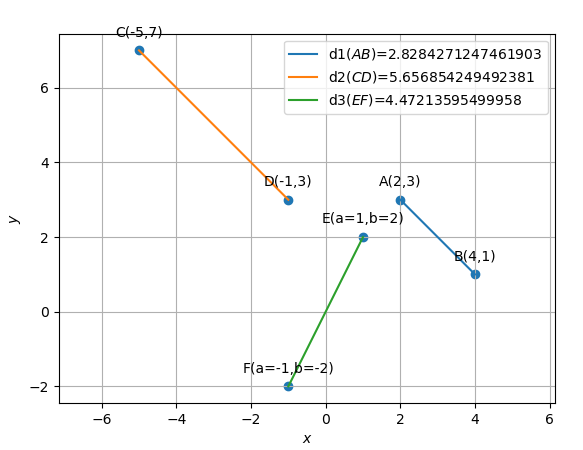
\includegraphics[width=0.75\columnwidth]{chapters/10/7/1/1/figs/graph.png}
	    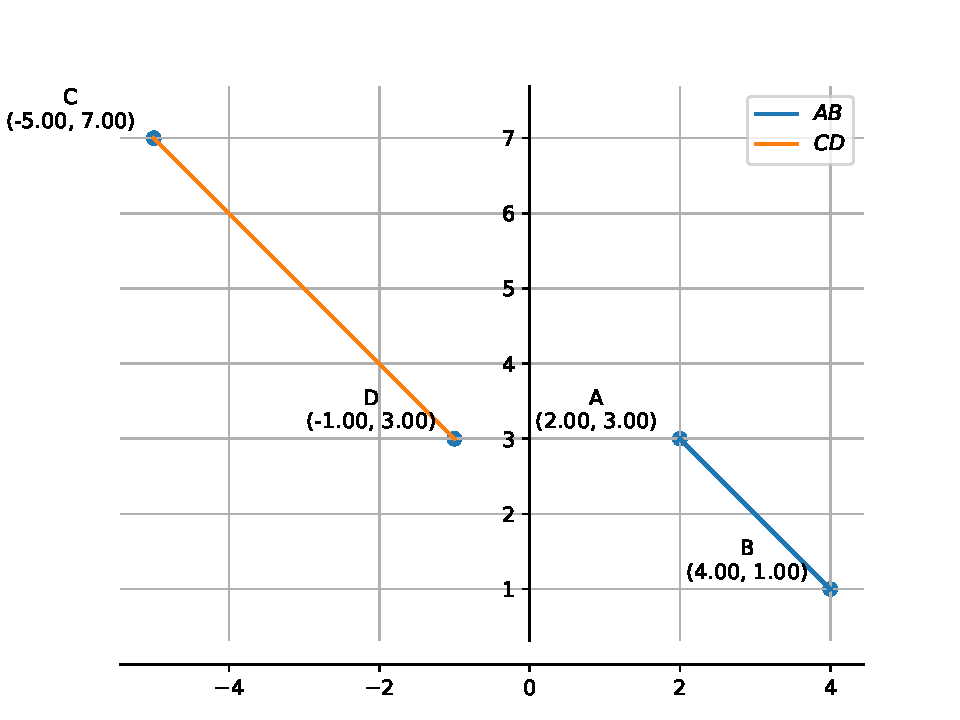
\includegraphics[width=0.75\columnwidth]{chapters/10/7/1/1/figs/fig.pdf}
	\end{center}
\caption{}
\label{fig:10/7/1/1Fig}
\end{figure}
\fi
\end{enumerate}

\item Find the distance between the points $(0, 0)$ and $ (36, 15)$.
	\\
		\solution
		%\renewcommand{\theequation}{\theenumi}
\begin{enumerate}[label=\thesubsection.\arabic*.,ref=\thesubsection.\theenumi]
%\numberwithin{equation}{enumi}
\item The direction vector of $AB$ is defined as
		\begin{align}
			\vec{B}-
			\vec{A}
		\end{align}
Find the direction vectors of $AB, BC$ and $CA$.
\\
\solution 
\begin{enumerate} 
\item  The Direction vector of $AB$ is 
	\begin{align}  \vec{B} - \vec{A} 
		=\myvec{ -4\\ 6 } - \myvec{ 1\\ -1 }
 = \myvec{ -4 - 1\\ 6 - (-1) } = \myvec{ -5\\ 7 }
		\label{eq:app-geo-dir-vec-ab}
 \end{align}
\item The Direction vector of $BC$ is
	\begin{align} \vec{C} - \vec{B}=\myvec{ -3\\ -5} - \myvec{ -4\\ 6 }
 = \myvec{ -3 - (-4)\\ -5 - 6 } = \myvec{1\\ -11 }
		\label{eq:app-geo-dir-vec-bc}
  \end{align}
  \item  The Direction vector of $CA$  is
	  \begin{align}  \vec{A} - \vec{C} =\myvec{ 1\\ -1 }-\myvec{ -3\\ -5}
 = \myvec{ 1 - (-3)\\ -1 - (-5) } = \myvec{ 4\\ 4 }
		\label{eq:app-geo-dir-vec-ca}
  \end{align}
 \end{enumerate}
%	\solution 
\begin{enumerate} 
\item  The Direction vector of $AB$ is 
	\begin{align}  \vec{B} - \vec{A} 
		=\myvec{ -4\\ 6 } - \myvec{ 1\\ -1 }
 = \myvec{ -4 - 1\\ 6 - (-1) } = \myvec{ -5\\ 7 }
		\label{eq:geo-dir-vec-ab}
 \end{align}
\item The Direction vector of $BC$ is
	\begin{align} \vec{C} - \vec{B}=\myvec{ -3\\ -5} - \myvec{ -4\\ 6 }
 = \myvec{ -3 - (-4)\\ -5 - 6 } = \myvec{1\\ -11 }
		\label{eq:geo-dir-vec-bc}
  \end{align}
  \item  The Direction vector of $CA$  is
	  \begin{align}  \vec{A} - \vec{C} =\myvec{ 1\\ -1 }-\myvec{ -3\\ -5}
 = \myvec{ 1 - (-3)\\ -1 - (-5) } = \myvec{ 4\\ 4 }
		\label{eq:geo-dir-vec-ca}
  \end{align}
 \end{enumerate}


	\item The length of side $BC$ is 
		\label{prob:side-length}
		\begin{align}
			c = \norm{\vec{B}-\vec{A}} \triangleq \sqrt{\brak{\vec{B}-\vec{A}}^{\top}\brak{\vec{B}-\vec{A}}}
		\end{align}
		where
		\begin{align}
			\vec{A}^{\top}\triangleq\myvec{1 & -1}
		\end{align}
		Similarly, 
		\begin{align}
b = \norm{\vec{C}-\vec{B}},\,
a = \norm{\vec{A}-\vec{C}}
		\end{align}
		Find $a, b, c$.
\begin{enumerate}
	\item 
	From 	
		\eqref{eq:app-geo-dir-vec-ab},
\begin{align}
\vec{A}-\vec{B} &= \myvec{5\\-7}, \\
\implies 	c &= 	\norm{\vec{B}-\vec{A}} = \norm{\vec{A}-\vec{B}} 
	\\
	&= \sqrt{\myvec{5 & -7}\myvec{5\\-7}}
= \sqrt{\brak{5}^2 +\brak{7}^2}\\
	&=\sqrt{74}
		\label{eq:app-geo-norm-ab}
\end{align}
	\item Similarly, from 
		\eqref{eq:app-geo-dir-vec-bc},
\begin{align}
	a &= \norm{\vec{B}-\vec{C}} 
	= \sqrt{\myvec{-1 & 11}\myvec{-1\\11}}
\\
&= \sqrt{\brak{1}^2+\brak{11}^2}
	= \sqrt{122}
		\label{eq:app-geo-norm-bc}
\end{align}
and
		from 		\eqref{eq:app-geo-dir-vec-ca},
	\item 
		\begin{align}
			b &= \norm{\vec{A}-\vec{C}} = \sqrt{\myvec{4 & 4}\myvec{4\\4}}
\\
&= \sqrt{\brak{4}^2+\brak{4}^2}
	=\sqrt{32}
		\label{eq:app-geo-norm-ca}
\end{align}
\end{enumerate}
%  \\            
  %\\ \solution 
\begin{align}
    \vec{A}-\vec{F}&=\myvec{1\\-1}-\myvec{\frac{-3}{2}\\\frac{5}{2}}
    =\myvec{\frac{5}{2}\\\frac{-7}{2}}
    \\
    \vec{E}-\vec{D}&=\myvec{-1\\-3}-\myvec{\frac{-7}{2}\\\frac{1}{2}}
    =\myvec{\frac{5}{2}\\\frac{-7}{2}}
    \\
	\implies	\vec{A}-\vec{F} &= \vec{E}-\vec{D}
\end{align}
See \figref{fig:Triangle-pgm}, 
\begin{figure}
\centering
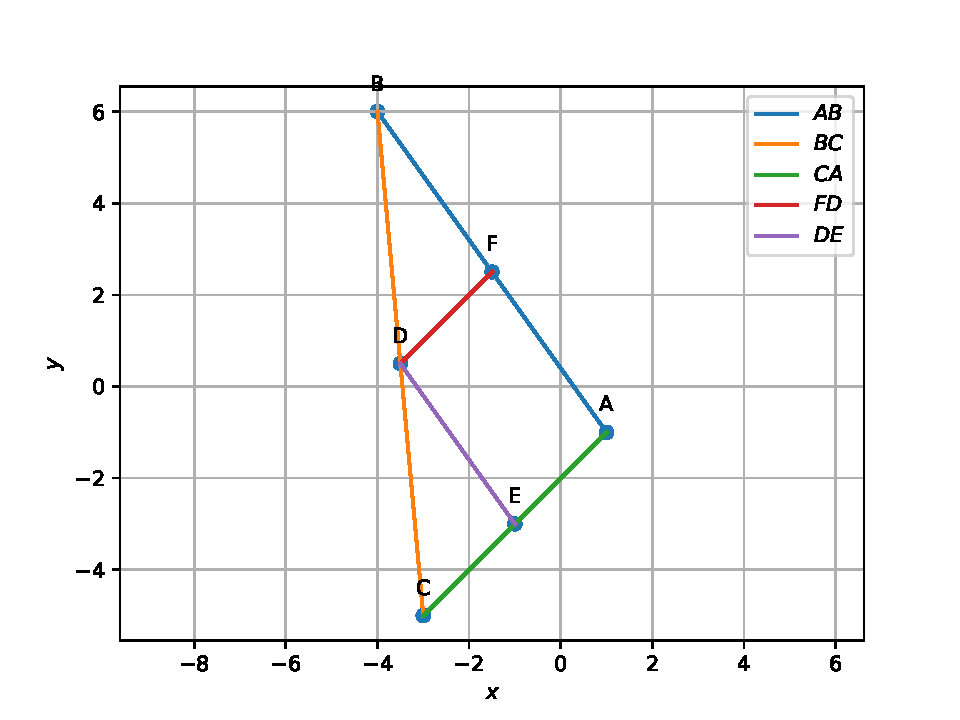
\includegraphics[width=0.75\columnwidth]{figs/triangle/pgm.pdf}
\caption{$AFDE$ forms a parallelogram in triangle ABC}
\label{fig:Triangle-pgm}
\end{figure}






















\item   Points $\vec{A}, \vec{B}, \vec{C}$ are defined to be collinear if 
		\begin{align}
			\label{eq:app-app-line-rank}
			\rank{\myvec{1 & 1 & 1 \\ \vec{A}& \vec{B}&\vec{C}}} = 2
		\end{align}
Are the given points in
			\eqref{eq:app-tri-pts}
collinear?
\\
\solution 
From 
			\eqref{eq:app-tri-pts},
\begin{align}
    \label{eq:app-1.1.3,2}
\myvec{
    1 & 1 & 1\\
    \vec{A} & \vec{B} & \vec{C} \\
    } 
    =
    %\label{eq:app-matthrowoperations}
    \myvec{
    1 & 1 & 1
    \\
    1 & -4 & -3
    \\
    -1 & 6 & -5
    }
     \xleftrightarrow[]{R_3 \leftarrow R_3+R_2}
    \myvec{
    1 & 1 & 1
    \\
    1 & -4 & -3
    \\
    0 & 2 & -8 
    }
    \\
     \xleftrightarrow[]{R_2\leftarrow R_1-R_2}
    \myvec{
    1 & 1 & 1
    \\
    0 & 5 & 4
    \\
    0 & 2 & -8 
    }
     \xleftrightarrow[]{R_3\leftarrow R_3-\frac{2}{5}R_2}
    \myvec{
    1 & 1 & 1
    \\
    0 & 5 & 4
    \\
    0 & 0 & \frac{-48}{5}
    }
\end{align}
There are no zero rows. So,
\begin{align}
    \text{rank}\myvec{
    1 & 1 & 1\\
    \vec{A} & \vec{B} & \vec{C} \\
    } &= 3 
\end{align}  
Hence,  the points $\vec{A},\vec{B},\vec{C}$ are not collinear. 
This is visible in 
\figref{fig1:Triangle}.
\begin{figure}[H]
\centering
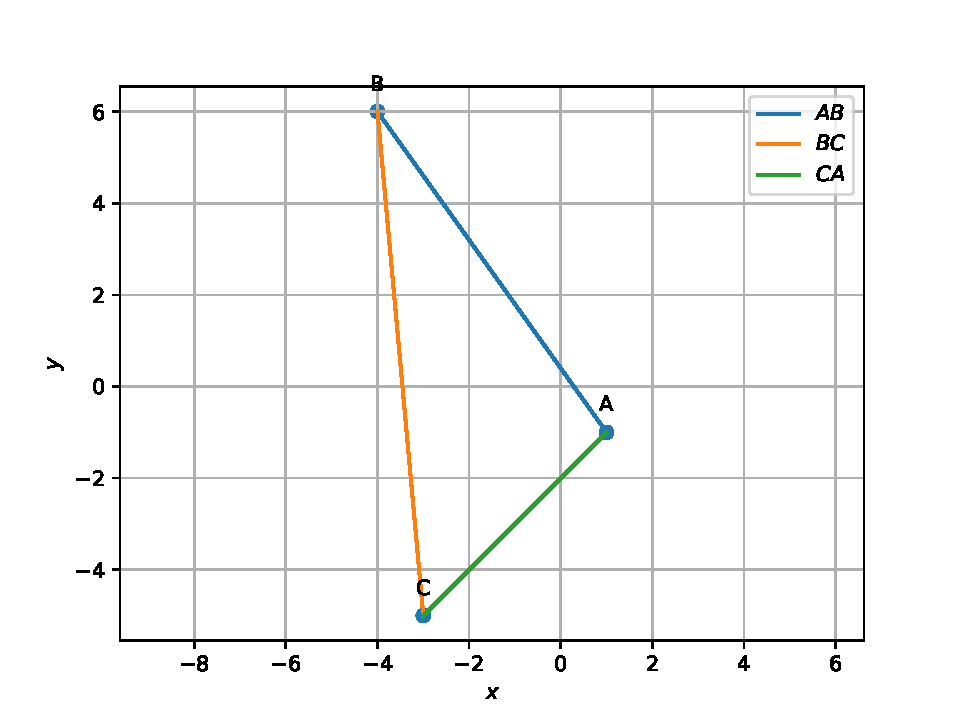
\includegraphics[width=0.75\columnwidth]{figs/triangle/vector.pdf}
\caption{$\triangle ABC$}
\label{fig1:Triangle}
\end{figure}
% \\		\\ \solution 
\begin{align}
    \vec{A}-\vec{F}&=\myvec{1\\-1}-\myvec{\frac{-3}{2}\\\frac{5}{2}}
    =\myvec{\frac{5}{2}\\\frac{-7}{2}}
    \\
    \vec{E}-\vec{D}&=\myvec{-1\\-3}-\myvec{\frac{-7}{2}\\\frac{1}{2}}
    =\myvec{\frac{5}{2}\\\frac{-7}{2}}
    \\
	\implies	\vec{A}-\vec{F} &= \vec{E}-\vec{D}
\end{align}
See \figref{fig:Triangle-pgm}, 
\begin{figure}
\centering
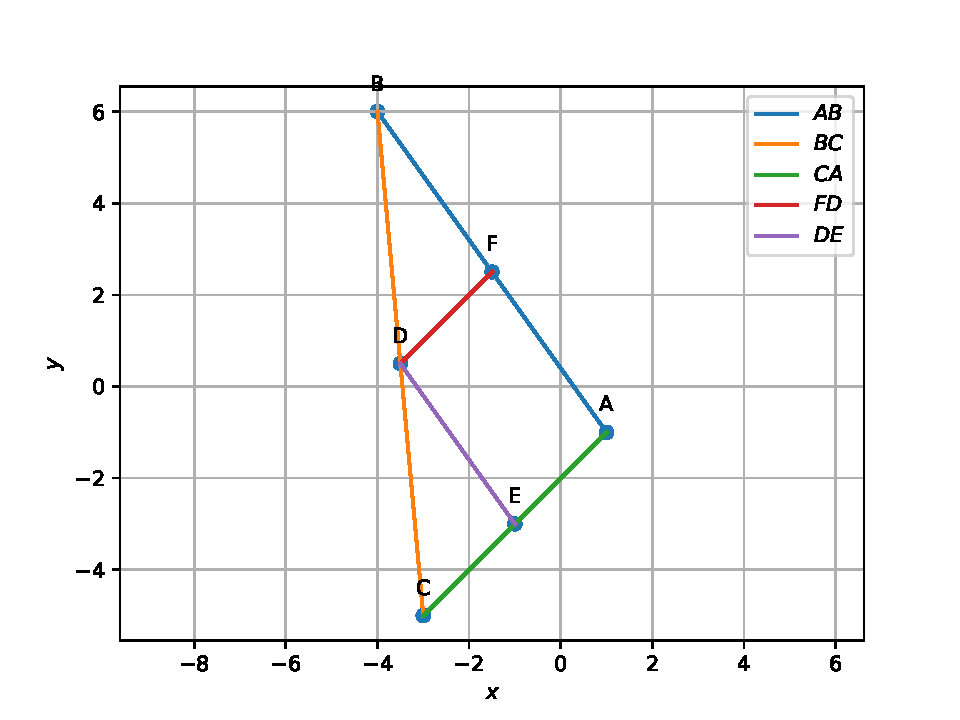
\includegraphics[width=0.75\columnwidth]{figs/triangle/pgm.pdf}
\caption{$AFDE$ forms a parallelogram in triangle ABC}
\label{fig:Triangle-pgm}
\end{figure}






















\item The parameteric form of the equation  of $AB$ is 
		\begin{align}
			\label{eq:app-geo-param}
			\vec{x}=\vec{A}+k\vec{m} \quad k \ne 0,
		\end{align}
		where
		\begin{align}
\vec{m}=\vec{B}-\vec{A}
		\end{align}
is the direction vector of $AB$.
Find the parameteric equations of $AB, BC$ and $CA$.
\\
\solution
From 
			\eqref{eq:app-geo-param} and
		\eqref{eq:app-geo-dir-vec-ab},
the parametric equation for $AB$ is given by
\begin{align}
AB: \vec{x} = &\myvec{1\\-1} + k \myvec{-5\\7}
\end{align}
Similarly, from 
		\eqref{eq:app-geo-dir-vec-bc} and
		\eqref{eq:app-geo-dir-vec-ca},
\begin{align}
BC: \vec{x} = &\myvec{-4\\6} + k \myvec{1\\-11}\\
CA: \vec{x} = &\myvec{-3\\-5} + k \myvec{4\\4}
\end{align}

%		\\ \solution 
\begin{align}
    \vec{A}-\vec{F}&=\myvec{1\\-1}-\myvec{\frac{-3}{2}\\\frac{5}{2}}
    =\myvec{\frac{5}{2}\\\frac{-7}{2}}
    \\
    \vec{E}-\vec{D}&=\myvec{-1\\-3}-\myvec{\frac{-7}{2}\\\frac{1}{2}}
    =\myvec{\frac{5}{2}\\\frac{-7}{2}}
    \\
	\implies	\vec{A}-\vec{F} &= \vec{E}-\vec{D}
\end{align}
See \figref{fig:Triangle-pgm}, 
\begin{figure}
\centering
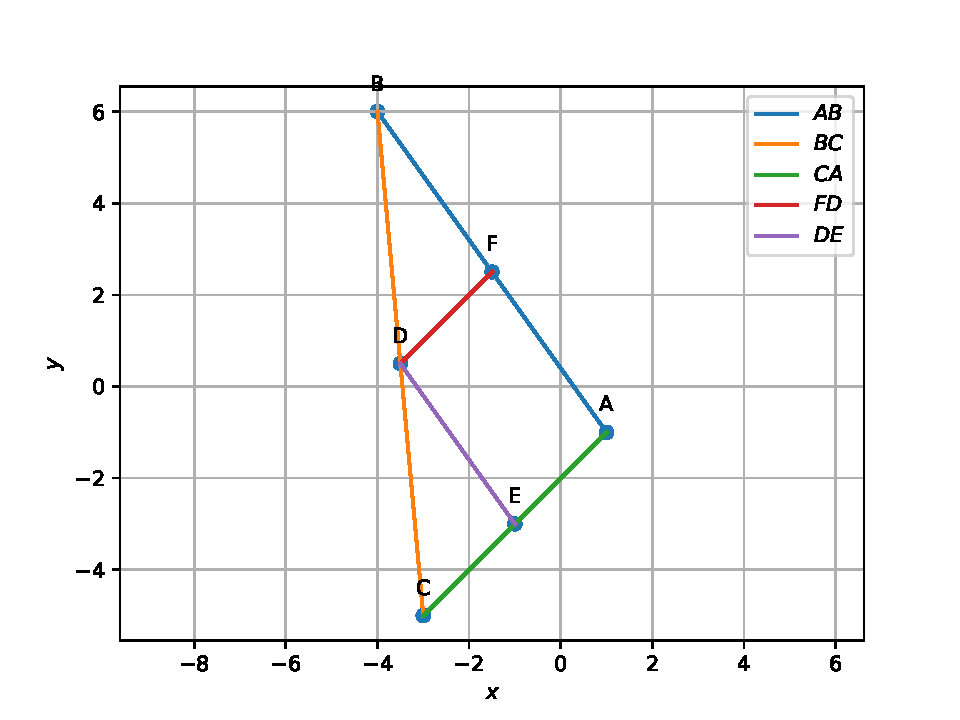
\includegraphics[width=0.75\columnwidth]{figs/triangle/pgm.pdf}
\caption{$AFDE$ forms a parallelogram in triangle ABC}
\label{fig:Triangle-pgm}
\end{figure}






















\item The normal form of the equation of $AB$  is 
		\begin{align}
			\label{eq:app-geo-normal}
			\vec{n}^{\top}\brak{	\vec{x}-\vec{A}} = 0
		\end{align}
		where 
		\begin{align}
			\vec{n}^{\top}\vec{m}&=\vec{n}^{\top}\brak{\vec{B}-\vec{A}} = 0
			\\
			\text{or, } \vec{n}&=\myvec{0 & 1 \\ -1 & 0} \vec{m}
			\label{eq:app-geo-norm-vec}
		\end{align}
Find the normal form of the equations of $AB, BC$ and $CA$.
\\
\solution
\begin{enumerate}
	\item
From
		\eqref{eq:app-geo-dir-vec-bc}, 
the direction vector of side $\vec{BC}$ is
\begin{align}
\vec{m}
	&=\myvec{1\\-11}
	\\
\implies \vec{n} &= \myvec{0 & 1\\
  -1 & 0}\myvec{1\\-11}
 = \myvec{-11\\-1}
		\label{eq:app-geo-norm-vec-bc}
\end{align}
from 
			\eqref{eq:app-geo-norm-vec}.
Hence, from 
			\eqref{eq:app-geo-normal},
the normal equation of side $BC$ is 
\begin{align}
	\vec{n}^{\top}\brak{	\vec{x}-\vec{B}} &= 0
			\\
\implies    \myvec{-11 & -1}\vec{x}&=\myvec{-11 & -1}\myvec{-4\\6}\\
    \implies
BC: \quad    \myvec{11 & 1}\vec{x}&=-38
\end{align}
\item Similarly, for $AB$,
from 
		\eqref{eq:app-geo-dir-vec-ab}, 
\begin{align}
	\vec{m} &= \myvec{-5\\7}
	\\
\implies        \vec{n} 
                &= \myvec{0&1\\-1&0}\myvec{-5\\7}
                = \myvec{7\\5}
		\label{eq:app-geo-norm-vec-ab}
\end{align}
and 
\begin{align}
	\vec{n}^{\top}\brak{	\vec{x}-\vec{A}} &= 0
	\\
	\implies
                AB: \quad  \vec{n}^{\top}\vec{x} &= \myvec{7&5}\myvec{1\\-1}\\    
       \implies\myvec{7&5}\vec{x} &= 2
\end{align}
\item For 
$CA$, 
from 
		\eqref{eq:app-geo-dir-vec-ca}, 
\begin{align}
\vec{m} &= \myvec{1 \\ 1}
\\
		\label{eq:app-geo-norm-vec-ca}
\implies \vec{n} 
&= \myvec{0&1 \\ -1&0}\myvec{1 \\ 1}
= \myvec{1 \\ -1}\\
\\
\implies	\vec{n}^{\top}\brak{	\vec{x}-\vec{C}} &= 0
\\
\implies \myvec{1&-1}{\vec{x}} &= \myvec{1&-1}\myvec{-3 \\ -5} 
= 2 
\end{align}
\end{enumerate}

%\begin{enumerate}
	\item
From
		\eqref{eq:geo-dir-vec-bc}, 
the direction vector of side $\vec{BC}$ is
\begin{align}
\vec{m}
	&=\myvec{1\\-11}
	\\
\implies \vec{n} &= \myvec{0 & 1\\
  -1 & 0}\myvec{1\\-11}
 = \myvec{-11\\-1}
		\label{eq:geo-norm-vec-bc}
\end{align}
from 
			\eqref{eq:geo-norm-vec}.
Hence, from 
			\eqref{eq:geo-normal},
the normal equation of side $BC$ is 
\begin{align}
	\vec{n}^{\top}\brak{	\vec{x}-\vec{B}} &= 0
			\\
\implies    \myvec{-11 & -1}\vec{x}&=\myvec{-11 & -1}\myvec{-4\\6}\\
    \implies
BC: \quad    \myvec{11 & 1}\vec{x}&=-38
\end{align}
\item Similarly, for $AB$,
from 
		\eqref{eq:geo-dir-vec-ab}, 
\begin{align}
	\vec{m} &= \myvec{-5\\7}
	\\
\implies        \vec{n} 
                &= \myvec{0&1\\-1&0}\myvec{-5\\7}
                = \myvec{7\\5}
		\label{eq:geo-norm-vec-ab}
\end{align}
and 
\begin{align}
	\vec{n}^{\top}\brak{	\vec{x}-\vec{A}} &= 0
	\\
	\implies
                AB: \quad  \vec{n}^{\top}\vec{x} &= \myvec{7&5}\myvec{1\\-1}\\    
       \implies\myvec{7&5}\vec{x} &= 2
\end{align}
\item For 
$CA$, 
from 
		\eqref{eq:geo-dir-vec-ca}, 
\begin{align}
\vec{m} &= \myvec{1 \\ 1}
\\
		\label{eq:geo-norm-vec-ca}
\implies \vec{n} 
&= \myvec{0&1 \\ -1&0}\myvec{1 \\ 1}
= \myvec{1 \\ -1}\\
\\
\implies	\vec{n}^{\top}\brak{	\vec{x}-\vec{C}} &= 0
\\
\implies \myvec{1&-1}{\vec{x}} &= \myvec{1&-1}\myvec{-3 \\ -5} 
= 2 
\end{align}
\end{enumerate}


\item The area of $\triangle ABC$ is defined as
		\begin{align}
			\label{eq:app-tri-area-cross}
			\frac{1}{2}\norm{{\brak{\vec{A}-\vec{B}}\times \brak{\vec{A}-\vec{C}}}}
		\end{align}
		where
		\begin{align}
			\vec{A}\times\vec{B} \triangleq \mydet{1 & -4 \\-1 & 6}
		\end{align}
		Find the area of $\triangle ABC$.\\
\solution
From
		\eqref{eq:app-geo-dir-vec-ab}
		and
		\eqref{eq:app-geo-dir-vec-ca},
\begin{align}
	\vec{A}-\vec{B}=\myvec{5\\-7},
	\vec{A}-\vec{C}&=\myvec{4\\4}\\
\implies (\vec{A}-\vec{B})\times(\vec{A}-\vec{C}) &=\mydet{5 & 4\\-7 & 4}\\
&=5\times 4-4\times (-7)\\&=48\\
\implies\frac{1}{2}\norm{(\vec{A}-\vec{B})\times(\vec{A}-\vec{C})}&=\frac{48}{2}=24
\end{align}
which is the desired area.

%  		\\ \solution 
\begin{align}
    \vec{A}-\vec{F}&=\myvec{1\\-1}-\myvec{\frac{-3}{2}\\\frac{5}{2}}
    =\myvec{\frac{5}{2}\\\frac{-7}{2}}
    \\
    \vec{E}-\vec{D}&=\myvec{-1\\-3}-\myvec{\frac{-7}{2}\\\frac{1}{2}}
    =\myvec{\frac{5}{2}\\\frac{-7}{2}}
    \\
	\implies	\vec{A}-\vec{F} &= \vec{E}-\vec{D}
\end{align}
See \figref{fig:Triangle-pgm}, 
\begin{figure}
\centering
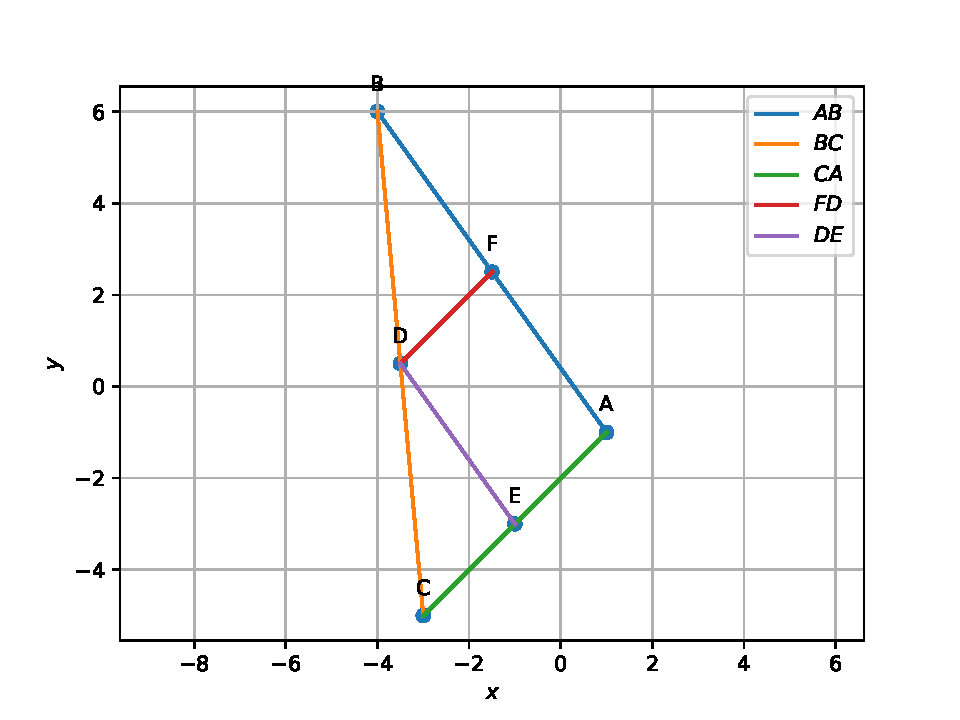
\includegraphics[width=0.75\columnwidth]{figs/triangle/pgm.pdf}
\caption{$AFDE$ forms a parallelogram in triangle ABC}
\label{fig:Triangle-pgm}
\end{figure}






















	\item Find the angles $A, B, C$ if 
%    \label{prop:angle2d}
  \begin{align}
    \label{eq:app-angle2d}
			\cos A \triangleq 
\frac{\brak{\vec{B}-\vec{A}}^{\top}{\vec{C}-\vec{A}}}{\norm{\vec{B}-\vec{A}}\norm{\vec{C}-\vec{A}}}
  \end{align}\\
  \solution
\begin{enumerate}
	\item From 
		\eqref{eq:app-geo-dir-vec-ab},
		\eqref{eq:app-geo-dir-vec-ca},
		\eqref{eq:app-geo-norm-ab}
		and
		\eqref{eq:app-geo-norm-ca}
\begin{align}
	(\vec{B}-\vec{A})^{\top}(\vec{C}-\vec{A})&=\myvec{-5&7}\myvec{-4\\-4}\\
	&=-8
	\\
	\implies
	\cos{A}&= \frac{-8}{\sqrt{74} \sqrt{32}}
	= \frac{-1}{\sqrt{37}}\\
	\implies A&=\cos^{-1}{\frac{-1}{\sqrt{37}}}
\end{align}
	\item From 
		\eqref{eq:app-geo-dir-vec-ab},
		\eqref{eq:app-geo-dir-vec-bc},
		\eqref{eq:app-geo-norm-ab}
		and
		\eqref{eq:app-geo-norm-bc}
\begin{align}
	(\vec{C}-\vec{B})^{\top}(\vec{A}-\vec{B})&=\myvec{1&-11}\myvec{5\\-7}\\
	&= 82
	\\
	\implies
	\cos{B}&= \frac{82}{\sqrt{74} \sqrt{122}}
	= \frac{41}{\sqrt{2257}}\\
	\implies B&=\cos^{-1}{\frac{41}{\sqrt{2257}}}
\end{align}
	\item From 
		\eqref{eq:app-geo-dir-vec-bc},
		\eqref{eq:app-geo-dir-vec-ca},
		\eqref{eq:app-geo-norm-bc}
		and
		\eqref{eq:app-geo-norm-ca}
\begin{align}
	(\vec{A}-\vec{C})^{\top}(\vec{B}-\vec{C})&=\myvec{4&4}\myvec{-1\\11}\\
	&=40
	\\
\implies	\cos{C}&= \frac{40}{\sqrt{32} \sqrt{122}}
	= \frac{5}{\sqrt{61}}\\
	\implies C&=\cos^{-1}{\frac{5}{\sqrt{61}}}
\end{align}

\end{enumerate}
%  	\\ \solution 
\begin{align}
    \vec{A}-\vec{F}&=\myvec{1\\-1}-\myvec{\frac{-3}{2}\\\frac{5}{2}}
    =\myvec{\frac{5}{2}\\\frac{-7}{2}}
    \\
    \vec{E}-\vec{D}&=\myvec{-1\\-3}-\myvec{\frac{-7}{2}\\\frac{1}{2}}
    =\myvec{\frac{5}{2}\\\frac{-7}{2}}
    \\
	\implies	\vec{A}-\vec{F} &= \vec{E}-\vec{D}
\end{align}
See \figref{fig:Triangle-pgm}, 
\begin{figure}
\centering
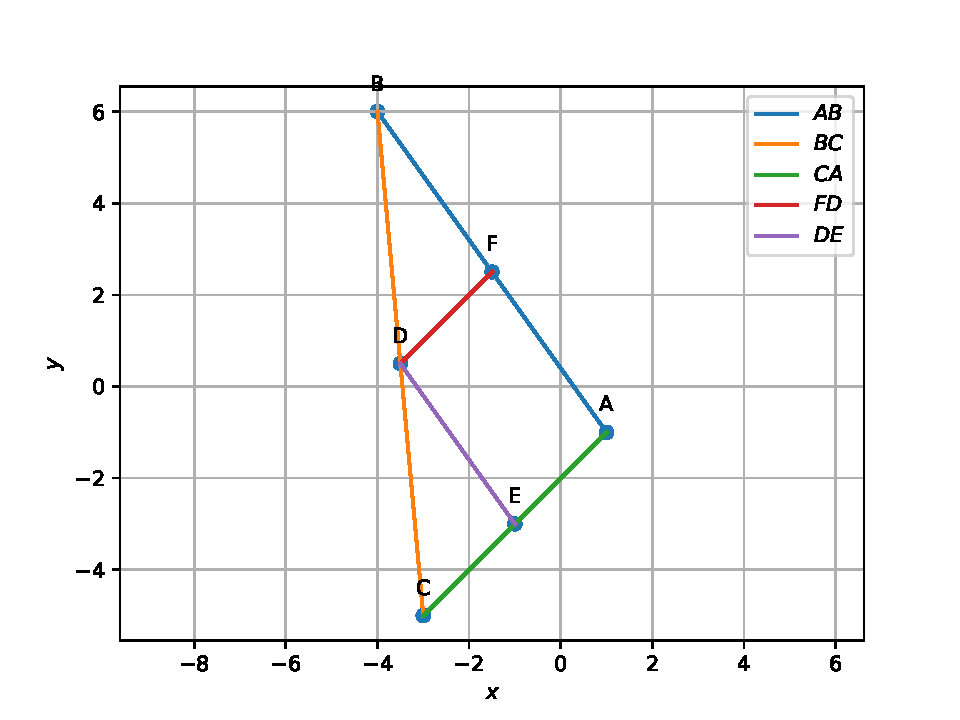
\includegraphics[width=0.75\columnwidth]{figs/triangle/pgm.pdf}
\caption{$AFDE$ forms a parallelogram in triangle ABC}
\label{fig:Triangle-pgm}
\end{figure}






















All codes for this section are available at
\begin{lstlisting}
	codes/triangle/sides.py
\end{lstlisting}
\end{enumerate}

\item Find the point on the X axis which is equidistant from $(2, -5)$ and $(-2, 9)$.
	\label{it:10/7/1/7}
	\\
\solution
		%\renewcommand{\theequation}{\theenumi}
\begin{enumerate}[label=\thesubsection.\arabic*.,ref=\thesubsection.\theenumi]
%\numberwithin{equation}{enumi}
\item The direction vector of $AB$ is defined as
		\begin{align}
			\vec{B}-
			\vec{A}
		\end{align}
Find the direction vectors of $AB, BC$ and $CA$.
\\
\solution 
\begin{enumerate} 
\item  The Direction vector of $AB$ is 
	\begin{align}  \vec{B} - \vec{A} 
		=\myvec{ -4\\ 6 } - \myvec{ 1\\ -1 }
 = \myvec{ -4 - 1\\ 6 - (-1) } = \myvec{ -5\\ 7 }
		\label{eq:app-geo-dir-vec-ab}
 \end{align}
\item The Direction vector of $BC$ is
	\begin{align} \vec{C} - \vec{B}=\myvec{ -3\\ -5} - \myvec{ -4\\ 6 }
 = \myvec{ -3 - (-4)\\ -5 - 6 } = \myvec{1\\ -11 }
		\label{eq:app-geo-dir-vec-bc}
  \end{align}
  \item  The Direction vector of $CA$  is
	  \begin{align}  \vec{A} - \vec{C} =\myvec{ 1\\ -1 }-\myvec{ -3\\ -5}
 = \myvec{ 1 - (-3)\\ -1 - (-5) } = \myvec{ 4\\ 4 }
		\label{eq:app-geo-dir-vec-ca}
  \end{align}
 \end{enumerate}
%	\solution 
\begin{enumerate} 
\item  The Direction vector of $AB$ is 
	\begin{align}  \vec{B} - \vec{A} 
		=\myvec{ -4\\ 6 } - \myvec{ 1\\ -1 }
 = \myvec{ -4 - 1\\ 6 - (-1) } = \myvec{ -5\\ 7 }
		\label{eq:geo-dir-vec-ab}
 \end{align}
\item The Direction vector of $BC$ is
	\begin{align} \vec{C} - \vec{B}=\myvec{ -3\\ -5} - \myvec{ -4\\ 6 }
 = \myvec{ -3 - (-4)\\ -5 - 6 } = \myvec{1\\ -11 }
		\label{eq:geo-dir-vec-bc}
  \end{align}
  \item  The Direction vector of $CA$  is
	  \begin{align}  \vec{A} - \vec{C} =\myvec{ 1\\ -1 }-\myvec{ -3\\ -5}
 = \myvec{ 1 - (-3)\\ -1 - (-5) } = \myvec{ 4\\ 4 }
		\label{eq:geo-dir-vec-ca}
  \end{align}
 \end{enumerate}


	\item The length of side $BC$ is 
		\label{prob:side-length}
		\begin{align}
			c = \norm{\vec{B}-\vec{A}} \triangleq \sqrt{\brak{\vec{B}-\vec{A}}^{\top}\brak{\vec{B}-\vec{A}}}
		\end{align}
		where
		\begin{align}
			\vec{A}^{\top}\triangleq\myvec{1 & -1}
		\end{align}
		Similarly, 
		\begin{align}
b = \norm{\vec{C}-\vec{B}},\,
a = \norm{\vec{A}-\vec{C}}
		\end{align}
		Find $a, b, c$.
\begin{enumerate}
	\item 
	From 	
		\eqref{eq:app-geo-dir-vec-ab},
\begin{align}
\vec{A}-\vec{B} &= \myvec{5\\-7}, \\
\implies 	c &= 	\norm{\vec{B}-\vec{A}} = \norm{\vec{A}-\vec{B}} 
	\\
	&= \sqrt{\myvec{5 & -7}\myvec{5\\-7}}
= \sqrt{\brak{5}^2 +\brak{7}^2}\\
	&=\sqrt{74}
		\label{eq:app-geo-norm-ab}
\end{align}
	\item Similarly, from 
		\eqref{eq:app-geo-dir-vec-bc},
\begin{align}
	a &= \norm{\vec{B}-\vec{C}} 
	= \sqrt{\myvec{-1 & 11}\myvec{-1\\11}}
\\
&= \sqrt{\brak{1}^2+\brak{11}^2}
	= \sqrt{122}
		\label{eq:app-geo-norm-bc}
\end{align}
and
		from 		\eqref{eq:app-geo-dir-vec-ca},
	\item 
		\begin{align}
			b &= \norm{\vec{A}-\vec{C}} = \sqrt{\myvec{4 & 4}\myvec{4\\4}}
\\
&= \sqrt{\brak{4}^2+\brak{4}^2}
	=\sqrt{32}
		\label{eq:app-geo-norm-ca}
\end{align}
\end{enumerate}
%  \\            
  %\\ \solution 
\begin{align}
    \vec{A}-\vec{F}&=\myvec{1\\-1}-\myvec{\frac{-3}{2}\\\frac{5}{2}}
    =\myvec{\frac{5}{2}\\\frac{-7}{2}}
    \\
    \vec{E}-\vec{D}&=\myvec{-1\\-3}-\myvec{\frac{-7}{2}\\\frac{1}{2}}
    =\myvec{\frac{5}{2}\\\frac{-7}{2}}
    \\
	\implies	\vec{A}-\vec{F} &= \vec{E}-\vec{D}
\end{align}
See \figref{fig:Triangle-pgm}, 
\begin{figure}
\centering
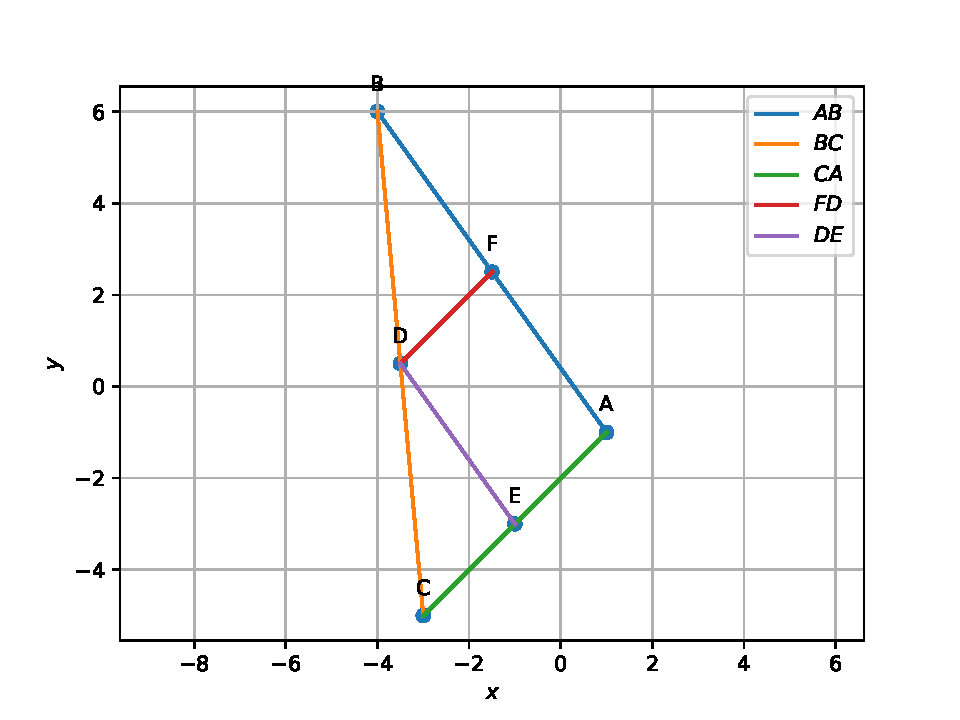
\includegraphics[width=0.75\columnwidth]{figs/triangle/pgm.pdf}
\caption{$AFDE$ forms a parallelogram in triangle ABC}
\label{fig:Triangle-pgm}
\end{figure}






















\item   Points $\vec{A}, \vec{B}, \vec{C}$ are defined to be collinear if 
		\begin{align}
			\label{eq:app-app-line-rank}
			\rank{\myvec{1 & 1 & 1 \\ \vec{A}& \vec{B}&\vec{C}}} = 2
		\end{align}
Are the given points in
			\eqref{eq:app-tri-pts}
collinear?
\\
\solution 
From 
			\eqref{eq:app-tri-pts},
\begin{align}
    \label{eq:app-1.1.3,2}
\myvec{
    1 & 1 & 1\\
    \vec{A} & \vec{B} & \vec{C} \\
    } 
    =
    %\label{eq:app-matthrowoperations}
    \myvec{
    1 & 1 & 1
    \\
    1 & -4 & -3
    \\
    -1 & 6 & -5
    }
     \xleftrightarrow[]{R_3 \leftarrow R_3+R_2}
    \myvec{
    1 & 1 & 1
    \\
    1 & -4 & -3
    \\
    0 & 2 & -8 
    }
    \\
     \xleftrightarrow[]{R_2\leftarrow R_1-R_2}
    \myvec{
    1 & 1 & 1
    \\
    0 & 5 & 4
    \\
    0 & 2 & -8 
    }
     \xleftrightarrow[]{R_3\leftarrow R_3-\frac{2}{5}R_2}
    \myvec{
    1 & 1 & 1
    \\
    0 & 5 & 4
    \\
    0 & 0 & \frac{-48}{5}
    }
\end{align}
There are no zero rows. So,
\begin{align}
    \text{rank}\myvec{
    1 & 1 & 1\\
    \vec{A} & \vec{B} & \vec{C} \\
    } &= 3 
\end{align}  
Hence,  the points $\vec{A},\vec{B},\vec{C}$ are not collinear. 
This is visible in 
\figref{fig1:Triangle}.
\begin{figure}[H]
\centering
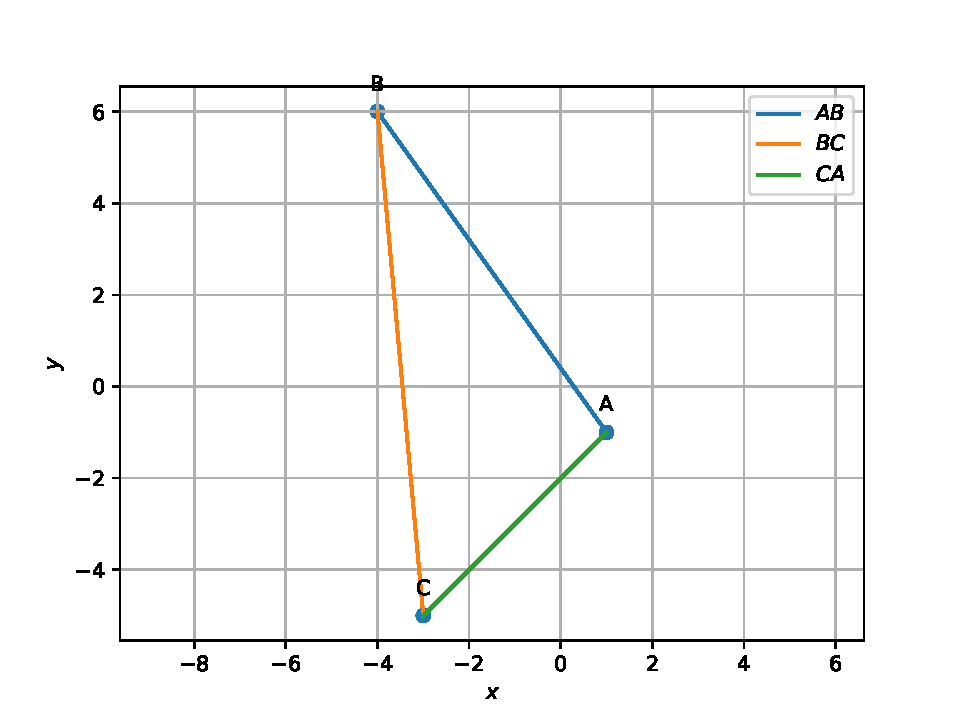
\includegraphics[width=0.75\columnwidth]{figs/triangle/vector.pdf}
\caption{$\triangle ABC$}
\label{fig1:Triangle}
\end{figure}
% \\		\\ \solution 
\begin{align}
    \vec{A}-\vec{F}&=\myvec{1\\-1}-\myvec{\frac{-3}{2}\\\frac{5}{2}}
    =\myvec{\frac{5}{2}\\\frac{-7}{2}}
    \\
    \vec{E}-\vec{D}&=\myvec{-1\\-3}-\myvec{\frac{-7}{2}\\\frac{1}{2}}
    =\myvec{\frac{5}{2}\\\frac{-7}{2}}
    \\
	\implies	\vec{A}-\vec{F} &= \vec{E}-\vec{D}
\end{align}
See \figref{fig:Triangle-pgm}, 
\begin{figure}
\centering
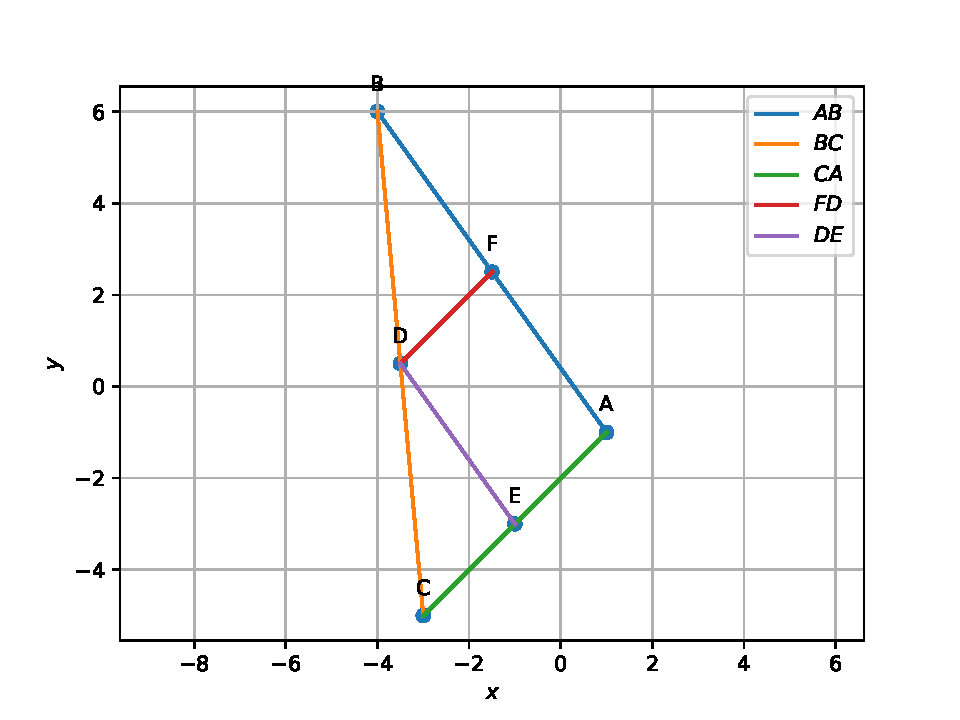
\includegraphics[width=0.75\columnwidth]{figs/triangle/pgm.pdf}
\caption{$AFDE$ forms a parallelogram in triangle ABC}
\label{fig:Triangle-pgm}
\end{figure}






















\item The parameteric form of the equation  of $AB$ is 
		\begin{align}
			\label{eq:app-geo-param}
			\vec{x}=\vec{A}+k\vec{m} \quad k \ne 0,
		\end{align}
		where
		\begin{align}
\vec{m}=\vec{B}-\vec{A}
		\end{align}
is the direction vector of $AB$.
Find the parameteric equations of $AB, BC$ and $CA$.
\\
\solution
From 
			\eqref{eq:app-geo-param} and
		\eqref{eq:app-geo-dir-vec-ab},
the parametric equation for $AB$ is given by
\begin{align}
AB: \vec{x} = &\myvec{1\\-1} + k \myvec{-5\\7}
\end{align}
Similarly, from 
		\eqref{eq:app-geo-dir-vec-bc} and
		\eqref{eq:app-geo-dir-vec-ca},
\begin{align}
BC: \vec{x} = &\myvec{-4\\6} + k \myvec{1\\-11}\\
CA: \vec{x} = &\myvec{-3\\-5} + k \myvec{4\\4}
\end{align}

%		\\ \solution 
\begin{align}
    \vec{A}-\vec{F}&=\myvec{1\\-1}-\myvec{\frac{-3}{2}\\\frac{5}{2}}
    =\myvec{\frac{5}{2}\\\frac{-7}{2}}
    \\
    \vec{E}-\vec{D}&=\myvec{-1\\-3}-\myvec{\frac{-7}{2}\\\frac{1}{2}}
    =\myvec{\frac{5}{2}\\\frac{-7}{2}}
    \\
	\implies	\vec{A}-\vec{F} &= \vec{E}-\vec{D}
\end{align}
See \figref{fig:Triangle-pgm}, 
\begin{figure}
\centering
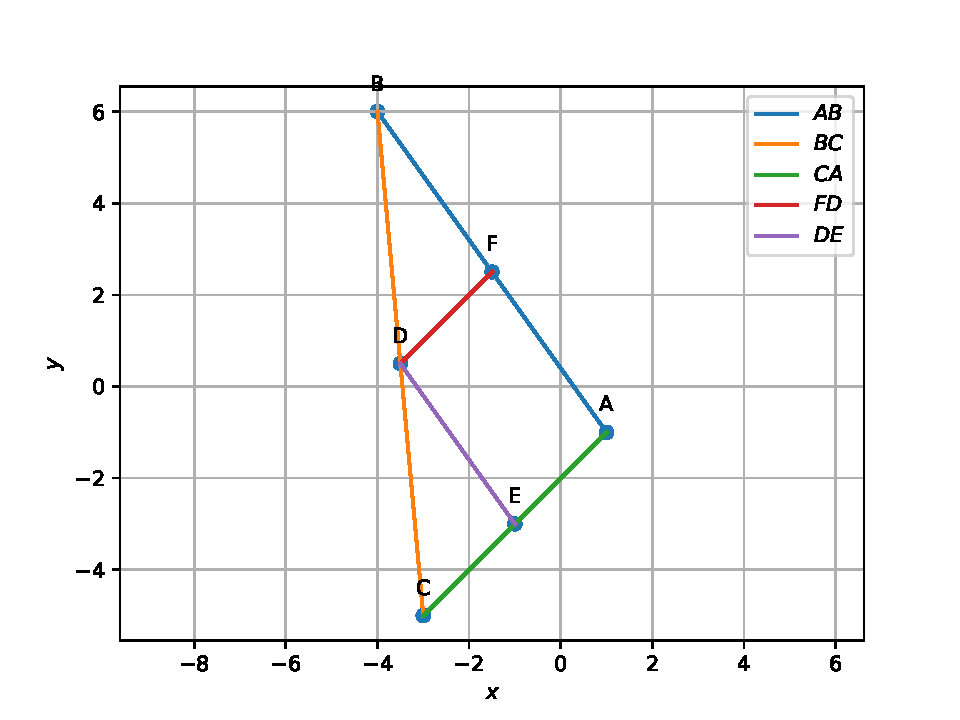
\includegraphics[width=0.75\columnwidth]{figs/triangle/pgm.pdf}
\caption{$AFDE$ forms a parallelogram in triangle ABC}
\label{fig:Triangle-pgm}
\end{figure}






















\item The normal form of the equation of $AB$  is 
		\begin{align}
			\label{eq:app-geo-normal}
			\vec{n}^{\top}\brak{	\vec{x}-\vec{A}} = 0
		\end{align}
		where 
		\begin{align}
			\vec{n}^{\top}\vec{m}&=\vec{n}^{\top}\brak{\vec{B}-\vec{A}} = 0
			\\
			\text{or, } \vec{n}&=\myvec{0 & 1 \\ -1 & 0} \vec{m}
			\label{eq:app-geo-norm-vec}
		\end{align}
Find the normal form of the equations of $AB, BC$ and $CA$.
\\
\solution
\begin{enumerate}
	\item
From
		\eqref{eq:app-geo-dir-vec-bc}, 
the direction vector of side $\vec{BC}$ is
\begin{align}
\vec{m}
	&=\myvec{1\\-11}
	\\
\implies \vec{n} &= \myvec{0 & 1\\
  -1 & 0}\myvec{1\\-11}
 = \myvec{-11\\-1}
		\label{eq:app-geo-norm-vec-bc}
\end{align}
from 
			\eqref{eq:app-geo-norm-vec}.
Hence, from 
			\eqref{eq:app-geo-normal},
the normal equation of side $BC$ is 
\begin{align}
	\vec{n}^{\top}\brak{	\vec{x}-\vec{B}} &= 0
			\\
\implies    \myvec{-11 & -1}\vec{x}&=\myvec{-11 & -1}\myvec{-4\\6}\\
    \implies
BC: \quad    \myvec{11 & 1}\vec{x}&=-38
\end{align}
\item Similarly, for $AB$,
from 
		\eqref{eq:app-geo-dir-vec-ab}, 
\begin{align}
	\vec{m} &= \myvec{-5\\7}
	\\
\implies        \vec{n} 
                &= \myvec{0&1\\-1&0}\myvec{-5\\7}
                = \myvec{7\\5}
		\label{eq:app-geo-norm-vec-ab}
\end{align}
and 
\begin{align}
	\vec{n}^{\top}\brak{	\vec{x}-\vec{A}} &= 0
	\\
	\implies
                AB: \quad  \vec{n}^{\top}\vec{x} &= \myvec{7&5}\myvec{1\\-1}\\    
       \implies\myvec{7&5}\vec{x} &= 2
\end{align}
\item For 
$CA$, 
from 
		\eqref{eq:app-geo-dir-vec-ca}, 
\begin{align}
\vec{m} &= \myvec{1 \\ 1}
\\
		\label{eq:app-geo-norm-vec-ca}
\implies \vec{n} 
&= \myvec{0&1 \\ -1&0}\myvec{1 \\ 1}
= \myvec{1 \\ -1}\\
\\
\implies	\vec{n}^{\top}\brak{	\vec{x}-\vec{C}} &= 0
\\
\implies \myvec{1&-1}{\vec{x}} &= \myvec{1&-1}\myvec{-3 \\ -5} 
= 2 
\end{align}
\end{enumerate}

%\begin{enumerate}
	\item
From
		\eqref{eq:geo-dir-vec-bc}, 
the direction vector of side $\vec{BC}$ is
\begin{align}
\vec{m}
	&=\myvec{1\\-11}
	\\
\implies \vec{n} &= \myvec{0 & 1\\
  -1 & 0}\myvec{1\\-11}
 = \myvec{-11\\-1}
		\label{eq:geo-norm-vec-bc}
\end{align}
from 
			\eqref{eq:geo-norm-vec}.
Hence, from 
			\eqref{eq:geo-normal},
the normal equation of side $BC$ is 
\begin{align}
	\vec{n}^{\top}\brak{	\vec{x}-\vec{B}} &= 0
			\\
\implies    \myvec{-11 & -1}\vec{x}&=\myvec{-11 & -1}\myvec{-4\\6}\\
    \implies
BC: \quad    \myvec{11 & 1}\vec{x}&=-38
\end{align}
\item Similarly, for $AB$,
from 
		\eqref{eq:geo-dir-vec-ab}, 
\begin{align}
	\vec{m} &= \myvec{-5\\7}
	\\
\implies        \vec{n} 
                &= \myvec{0&1\\-1&0}\myvec{-5\\7}
                = \myvec{7\\5}
		\label{eq:geo-norm-vec-ab}
\end{align}
and 
\begin{align}
	\vec{n}^{\top}\brak{	\vec{x}-\vec{A}} &= 0
	\\
	\implies
                AB: \quad  \vec{n}^{\top}\vec{x} &= \myvec{7&5}\myvec{1\\-1}\\    
       \implies\myvec{7&5}\vec{x} &= 2
\end{align}
\item For 
$CA$, 
from 
		\eqref{eq:geo-dir-vec-ca}, 
\begin{align}
\vec{m} &= \myvec{1 \\ 1}
\\
		\label{eq:geo-norm-vec-ca}
\implies \vec{n} 
&= \myvec{0&1 \\ -1&0}\myvec{1 \\ 1}
= \myvec{1 \\ -1}\\
\\
\implies	\vec{n}^{\top}\brak{	\vec{x}-\vec{C}} &= 0
\\
\implies \myvec{1&-1}{\vec{x}} &= \myvec{1&-1}\myvec{-3 \\ -5} 
= 2 
\end{align}
\end{enumerate}


\item The area of $\triangle ABC$ is defined as
		\begin{align}
			\label{eq:app-tri-area-cross}
			\frac{1}{2}\norm{{\brak{\vec{A}-\vec{B}}\times \brak{\vec{A}-\vec{C}}}}
		\end{align}
		where
		\begin{align}
			\vec{A}\times\vec{B} \triangleq \mydet{1 & -4 \\-1 & 6}
		\end{align}
		Find the area of $\triangle ABC$.\\
\solution
From
		\eqref{eq:app-geo-dir-vec-ab}
		and
		\eqref{eq:app-geo-dir-vec-ca},
\begin{align}
	\vec{A}-\vec{B}=\myvec{5\\-7},
	\vec{A}-\vec{C}&=\myvec{4\\4}\\
\implies (\vec{A}-\vec{B})\times(\vec{A}-\vec{C}) &=\mydet{5 & 4\\-7 & 4}\\
&=5\times 4-4\times (-7)\\&=48\\
\implies\frac{1}{2}\norm{(\vec{A}-\vec{B})\times(\vec{A}-\vec{C})}&=\frac{48}{2}=24
\end{align}
which is the desired area.

%  		\\ \solution 
\begin{align}
    \vec{A}-\vec{F}&=\myvec{1\\-1}-\myvec{\frac{-3}{2}\\\frac{5}{2}}
    =\myvec{\frac{5}{2}\\\frac{-7}{2}}
    \\
    \vec{E}-\vec{D}&=\myvec{-1\\-3}-\myvec{\frac{-7}{2}\\\frac{1}{2}}
    =\myvec{\frac{5}{2}\\\frac{-7}{2}}
    \\
	\implies	\vec{A}-\vec{F} &= \vec{E}-\vec{D}
\end{align}
See \figref{fig:Triangle-pgm}, 
\begin{figure}
\centering
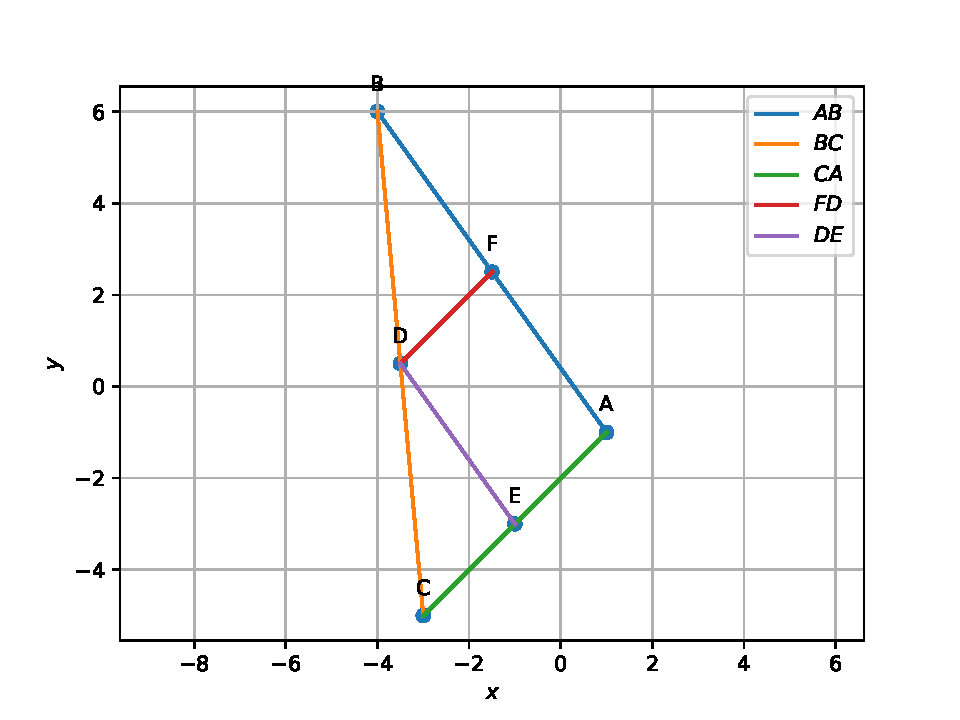
\includegraphics[width=0.75\columnwidth]{figs/triangle/pgm.pdf}
\caption{$AFDE$ forms a parallelogram in triangle ABC}
\label{fig:Triangle-pgm}
\end{figure}






















	\item Find the angles $A, B, C$ if 
%    \label{prop:angle2d}
  \begin{align}
    \label{eq:app-angle2d}
			\cos A \triangleq 
\frac{\brak{\vec{B}-\vec{A}}^{\top}{\vec{C}-\vec{A}}}{\norm{\vec{B}-\vec{A}}\norm{\vec{C}-\vec{A}}}
  \end{align}\\
  \solution
\begin{enumerate}
	\item From 
		\eqref{eq:app-geo-dir-vec-ab},
		\eqref{eq:app-geo-dir-vec-ca},
		\eqref{eq:app-geo-norm-ab}
		and
		\eqref{eq:app-geo-norm-ca}
\begin{align}
	(\vec{B}-\vec{A})^{\top}(\vec{C}-\vec{A})&=\myvec{-5&7}\myvec{-4\\-4}\\
	&=-8
	\\
	\implies
	\cos{A}&= \frac{-8}{\sqrt{74} \sqrt{32}}
	= \frac{-1}{\sqrt{37}}\\
	\implies A&=\cos^{-1}{\frac{-1}{\sqrt{37}}}
\end{align}
	\item From 
		\eqref{eq:app-geo-dir-vec-ab},
		\eqref{eq:app-geo-dir-vec-bc},
		\eqref{eq:app-geo-norm-ab}
		and
		\eqref{eq:app-geo-norm-bc}
\begin{align}
	(\vec{C}-\vec{B})^{\top}(\vec{A}-\vec{B})&=\myvec{1&-11}\myvec{5\\-7}\\
	&= 82
	\\
	\implies
	\cos{B}&= \frac{82}{\sqrt{74} \sqrt{122}}
	= \frac{41}{\sqrt{2257}}\\
	\implies B&=\cos^{-1}{\frac{41}{\sqrt{2257}}}
\end{align}
	\item From 
		\eqref{eq:app-geo-dir-vec-bc},
		\eqref{eq:app-geo-dir-vec-ca},
		\eqref{eq:app-geo-norm-bc}
		and
		\eqref{eq:app-geo-norm-ca}
\begin{align}
	(\vec{A}-\vec{C})^{\top}(\vec{B}-\vec{C})&=\myvec{4&4}\myvec{-1\\11}\\
	&=40
	\\
\implies	\cos{C}&= \frac{40}{\sqrt{32} \sqrt{122}}
	= \frac{5}{\sqrt{61}}\\
	\implies C&=\cos^{-1}{\frac{5}{\sqrt{61}}}
\end{align}

\end{enumerate}
%  	\\ \solution 
\begin{align}
    \vec{A}-\vec{F}&=\myvec{1\\-1}-\myvec{\frac{-3}{2}\\\frac{5}{2}}
    =\myvec{\frac{5}{2}\\\frac{-7}{2}}
    \\
    \vec{E}-\vec{D}&=\myvec{-1\\-3}-\myvec{\frac{-7}{2}\\\frac{1}{2}}
    =\myvec{\frac{5}{2}\\\frac{-7}{2}}
    \\
	\implies	\vec{A}-\vec{F} &= \vec{E}-\vec{D}
\end{align}
See \figref{fig:Triangle-pgm}, 
\begin{figure}
\centering
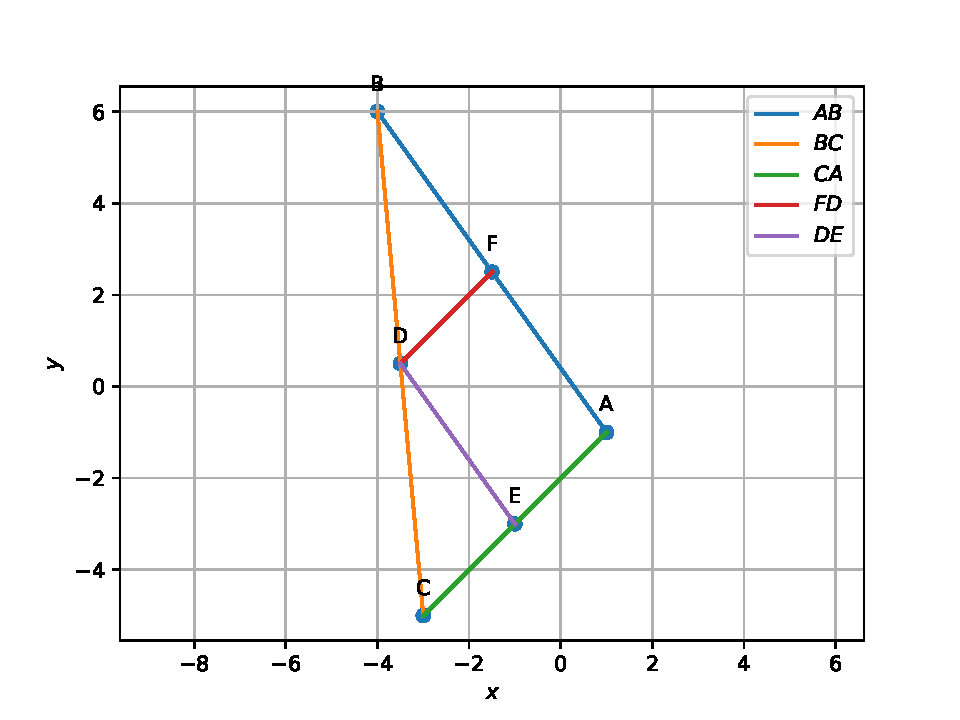
\includegraphics[width=0.75\columnwidth]{figs/triangle/pgm.pdf}
\caption{$AFDE$ forms a parallelogram in triangle ABC}
\label{fig:Triangle-pgm}
\end{figure}






















All codes for this section are available at
\begin{lstlisting}
	codes/triangle/sides.py
\end{lstlisting}
\end{enumerate}

\item Find the values of $y$ for which the distance between the points                  $\vec{P}(2, -3)$ and $\vec{Q}(10, y)$ is 10 units.
\item  If $\vec{Q}(0,  1)$ is equidistant from $\vec{P}(5,  -3)$ and $\vec{R}(x,  6)$,  find the values of $x$. Also find the
distances $QR$ and $PR$.
\item  Find a relation between $x$ and $y$ such that the point $(x, y)$ is equidistant from the point
$(3,  6)$ and $(– 3,  4)$.
	\item Find a point on the X axis, which is equidistant from the points $\myvec{
  7 \\
  6 \\
 }$ and $\myvec{
  3 \\
  4 \\
 }$
.
\label{chapters/11/10/1/4}
%	\\
%	\solution 
%The direction vector
\begin{align}
	\vec{B}-\vec{A}
	=
	\myvec{
  h-x_1\\
  k-y_1
  }
   \equiv
	\myvec{
1\\
	\frac{ k-y_1}{h-x_1}
  }
  \\
	\implies m = 
	\frac{ k-y_1}{h-x_1},
\end{align}
yielding the desired result.

\item The distance between the points $\vec{A}(0,  6) \text{ and } \vec{B}(0,  –2)$ is
\item The distance of the point $\vec{P} (–6,  8)$ from the origin is
\item The distance between the points $\vec(0,  5)\text{ and }(–5,  0)$ is
\item $AOBC$ is a rectangle whose three vertices are vertices $\vec{A} (0,  3),  \vec{O}(0,  0)\text{ and }
	\vec{B} (5,  0)$. The length of its diagonal is
\item The perimeter of a triangle with vertices $\vec(0,  4),  (0,  0) \text{ and } (3,  0)$ is
\item If the distance between the points $(4, P)$  and $ (1, 0)$ is 5, then the value of $P$ is
\item Find the points on the $X$ axis which are at a distance on $2\sqrt{5}$ from the point $ (7, -4).$ How many such points are there?
\item Find the value of $a$,  if the if the distance between the points $\vec{A}(-3, -14)$  and $\vec{B}(a, -5)$ is 9 units.
\item Find a point which is equidistant from the points $\vec{A}(-5, 4)$  and $(-1, 6)$.  How many such points are there ?
\item If the point $\vec{A}(2, -4)$ is equidistant from $\vec{P}(3, 8)$  and $\vec{Q}(-10, y)$,  find the values of $y$.  Also find distance $PQ$.
\item If $(a, b)$ is the mid-point of the line segment joining the point $\vec{A}(10, -6)\text{ and }\vec{B}(k, 4)$ and $a-2b=18$,  find the value of $a, b$ and the distance $AB$.
\item Find a relation between $x$ and $y$ such that the point $(x,y)$ is equidistant from the points $(7,1)$ and $(3,5)$.
\item Find a point on the Y axis which is equidistant from the points $\vec{A}(6,5)$ and $\vec{B}(-4,3)$.
\item Find the equation of set of points $\vec{P}$ such that $PA^2+PB^2=2k^2$, where $\vec{A}$ and $\vec{B}$ are the points $(3,4,5)$ and $(-1,3,-7)$, respectively.
\item Find the equation of the set of the points $\vec{P}$ such that its distances from the points $\vec{A}(3,4,-5)$ and $\vec{B}(-2,1,4)$ are equal.
\item Find a vector in the direction of vector $\overrightarrow{a}=\hat{i} -2\hat{j}$ that has magnitude $7$ units.
\end{enumerate}

\subsection{CBSE}
\begin{enumerate}[label=\thesubsection.\arabic*, ref=\thesubsection.\theenumi]
\item Compute the magnitude of the following vectors:
\begin{align}
	\vec{a}&=\hat{i}+\hat{j}+\hat{k}
	\\
	\vec{b}&=2\hat{i}-7\hat{j}-3\hat{k}
	\\
	\vec{c}&=\frac{1}{\sqrt{3}}\hat{i}+\frac{1}{\sqrt{3}}\hat{j}-\frac{1}{3}\hat{k}
\end{align}
    \solution 
		From the given information,
		\begin{align}
			\vec{a}=\myvec{\cos\frac{\pi}{3}\\\cos\frac{\pi}{4}\\\cos\theta}
			= 
\myvec{\frac{1}{2}\\[1ex]\frac{1}{\sqrt{2}}\\[1ex]\cos\theta}
		\end{align}
\begin{align}
\because    \norm{\vec{a}}&=1,
\\
\frac{1}{4}+\frac{1}{2}+\cos^2\theta&=1
\\
    \implies\cos\theta &=\frac{1}{2}
\end{align}
$\because \theta$ is an acute angle.
    Hence 
\begin{align}
		\vec{a}=\myvec{\frac{1}{2}\\[1ex] \frac{1}{\sqrt{2}}\\[1ex] \frac{1}{2}}
\end{align}

\item Find the distance between the following pairs of points
\begin{enumerate}[label=(\roman*)]
\item $(2, 3, 5)$ and $(4, 3, 1)$
\item $(-3, 7, 2)$ and $(2, 4, -1)$
\item $(-1, 3, -4)$ and $(1, -3, 4)$
\item $(2, -1, 3)$ and $(-2, 1, 3)$
\end{enumerate}
\item Find the lengths of the medians of the triangle with vertices $\vec{A}(0, 0, 6),  \vec{B}(0, 4, 0)$ and $\vec{C}(6, 0, 0)$.
\item Find the coordinates of a point on Y axis which is at a distance of $5\sqrt2$ from the point $\vec{P}(3, -2, 5)$.
\item If $\vec{A}$ and $\vec{B}$ be the points $(3, 4, 5)$ and $(-1, 3, -7)$ respectively,  find the equation of the set of the points $\vec{P}$ such that $PA^2+PB^2=K^2$ where $K$ is a constant.
\item Find the distances between the following pairs of points
\begin{enumerate}
\item $(2, 3), (4, 1)$
\item $(-5, 7), (-1, 3)$
\item $(a, b), (-a, -b)$
\end{enumerate}
\solution
		\begin{enumerate}
\item 
	\begin{align}
\because
		\vec{A} - \vec{B} = \myvec{2\\3} - \myvec{4\\1} &= \myvec{-2\\2},		
\\
(\vec{A}-\vec{B})^\top (\vec{A}-\vec{B}) &= 8
	\end{align}
	Thus, the desired distance is 
	\begin{align}
		d=\norm{\vec{A}-\vec{B}} =\sqrt{8}
	\end{align}
\item 
	\begin{align}
		\vec{C} - \vec{D} = \myvec{-5\\7} - \myvec{-1\\3} &= \myvec{-4\\4}		
		\\
		\implies		(\vec{C}-\vec{D})^\top (\vec{C}-\vec{D}) &= 32
	\end{align}
Thus,	
	\begin{align}
		d=\norm{\vec{C}-\vec{D}}
 =4\sqrt{2}
\end{align}	
%	
\item 
	\begin{align}
\vec{E} - \vec{F} = \myvec{a\\b} - \myvec{-a\\-b} &= \myvec{2a\\2b}		
		\\
		\implies
		(\vec{E}-\vec{F})^\top (\vec{E}-\vec{F}) = 4a^2+4b^2 
	\end{align}
Thus,	
	\begin{align}
		d=\norm{\vec{E}-\vec{F}} =
2\sqrt{a^2+b^2}
\end{align}	
\iffalse
\begin{figure}[H]
	\begin{center} 
	    %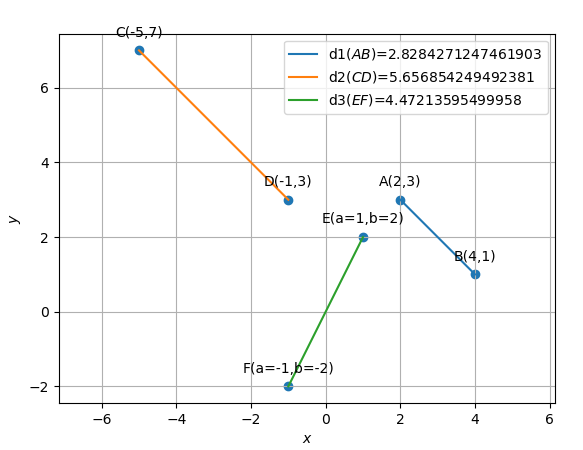
\includegraphics[width=0.75\columnwidth]{chapters/10/7/1/1/figs/graph.png}
	    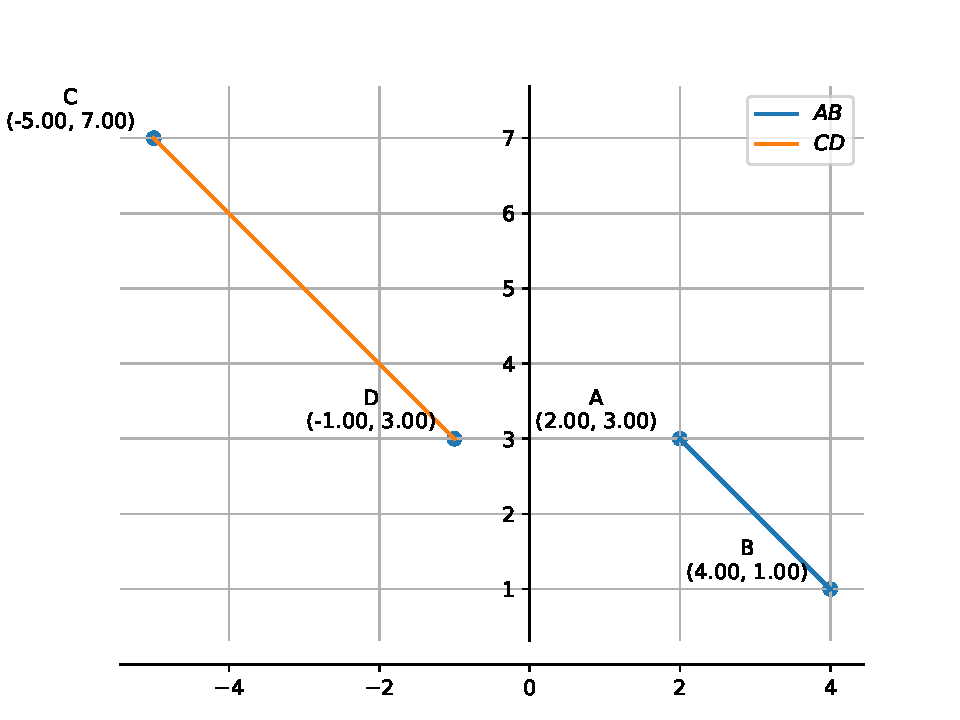
\includegraphics[width=0.75\columnwidth]{chapters/10/7/1/1/figs/fig.pdf}
	\end{center}
\caption{}
\label{fig:10/7/1/1Fig}
\end{figure}
\fi
\end{enumerate}

\item Find the distance between the points $(0, 0)$ and $ (36, 15)$.
	\\
		\solution
		%\renewcommand{\theequation}{\theenumi}
\begin{enumerate}[label=\thesubsection.\arabic*.,ref=\thesubsection.\theenumi]
%\numberwithin{equation}{enumi}
\item The direction vector of $AB$ is defined as
		\begin{align}
			\vec{B}-
			\vec{A}
		\end{align}
Find the direction vectors of $AB, BC$ and $CA$.
\\
\solution 
\begin{enumerate} 
\item  The Direction vector of $AB$ is 
	\begin{align}  \vec{B} - \vec{A} 
		=\myvec{ -4\\ 6 } - \myvec{ 1\\ -1 }
 = \myvec{ -4 - 1\\ 6 - (-1) } = \myvec{ -5\\ 7 }
		\label{eq:app-geo-dir-vec-ab}
 \end{align}
\item The Direction vector of $BC$ is
	\begin{align} \vec{C} - \vec{B}=\myvec{ -3\\ -5} - \myvec{ -4\\ 6 }
 = \myvec{ -3 - (-4)\\ -5 - 6 } = \myvec{1\\ -11 }
		\label{eq:app-geo-dir-vec-bc}
  \end{align}
  \item  The Direction vector of $CA$  is
	  \begin{align}  \vec{A} - \vec{C} =\myvec{ 1\\ -1 }-\myvec{ -3\\ -5}
 = \myvec{ 1 - (-3)\\ -1 - (-5) } = \myvec{ 4\\ 4 }
		\label{eq:app-geo-dir-vec-ca}
  \end{align}
 \end{enumerate}
%	\solution 
\begin{enumerate} 
\item  The Direction vector of $AB$ is 
	\begin{align}  \vec{B} - \vec{A} 
		=\myvec{ -4\\ 6 } - \myvec{ 1\\ -1 }
 = \myvec{ -4 - 1\\ 6 - (-1) } = \myvec{ -5\\ 7 }
		\label{eq:geo-dir-vec-ab}
 \end{align}
\item The Direction vector of $BC$ is
	\begin{align} \vec{C} - \vec{B}=\myvec{ -3\\ -5} - \myvec{ -4\\ 6 }
 = \myvec{ -3 - (-4)\\ -5 - 6 } = \myvec{1\\ -11 }
		\label{eq:geo-dir-vec-bc}
  \end{align}
  \item  The Direction vector of $CA$  is
	  \begin{align}  \vec{A} - \vec{C} =\myvec{ 1\\ -1 }-\myvec{ -3\\ -5}
 = \myvec{ 1 - (-3)\\ -1 - (-5) } = \myvec{ 4\\ 4 }
		\label{eq:geo-dir-vec-ca}
  \end{align}
 \end{enumerate}


	\item The length of side $BC$ is 
		\label{prob:side-length}
		\begin{align}
			c = \norm{\vec{B}-\vec{A}} \triangleq \sqrt{\brak{\vec{B}-\vec{A}}^{\top}\brak{\vec{B}-\vec{A}}}
		\end{align}
		where
		\begin{align}
			\vec{A}^{\top}\triangleq\myvec{1 & -1}
		\end{align}
		Similarly, 
		\begin{align}
b = \norm{\vec{C}-\vec{B}},\,
a = \norm{\vec{A}-\vec{C}}
		\end{align}
		Find $a, b, c$.
\begin{enumerate}
	\item 
	From 	
		\eqref{eq:app-geo-dir-vec-ab},
\begin{align}
\vec{A}-\vec{B} &= \myvec{5\\-7}, \\
\implies 	c &= 	\norm{\vec{B}-\vec{A}} = \norm{\vec{A}-\vec{B}} 
	\\
	&= \sqrt{\myvec{5 & -7}\myvec{5\\-7}}
= \sqrt{\brak{5}^2 +\brak{7}^2}\\
	&=\sqrt{74}
		\label{eq:app-geo-norm-ab}
\end{align}
	\item Similarly, from 
		\eqref{eq:app-geo-dir-vec-bc},
\begin{align}
	a &= \norm{\vec{B}-\vec{C}} 
	= \sqrt{\myvec{-1 & 11}\myvec{-1\\11}}
\\
&= \sqrt{\brak{1}^2+\brak{11}^2}
	= \sqrt{122}
		\label{eq:app-geo-norm-bc}
\end{align}
and
		from 		\eqref{eq:app-geo-dir-vec-ca},
	\item 
		\begin{align}
			b &= \norm{\vec{A}-\vec{C}} = \sqrt{\myvec{4 & 4}\myvec{4\\4}}
\\
&= \sqrt{\brak{4}^2+\brak{4}^2}
	=\sqrt{32}
		\label{eq:app-geo-norm-ca}
\end{align}
\end{enumerate}
%  \\            
  %\\ \solution 
\begin{align}
    \vec{A}-\vec{F}&=\myvec{1\\-1}-\myvec{\frac{-3}{2}\\\frac{5}{2}}
    =\myvec{\frac{5}{2}\\\frac{-7}{2}}
    \\
    \vec{E}-\vec{D}&=\myvec{-1\\-3}-\myvec{\frac{-7}{2}\\\frac{1}{2}}
    =\myvec{\frac{5}{2}\\\frac{-7}{2}}
    \\
	\implies	\vec{A}-\vec{F} &= \vec{E}-\vec{D}
\end{align}
See \figref{fig:Triangle-pgm}, 
\begin{figure}
\centering
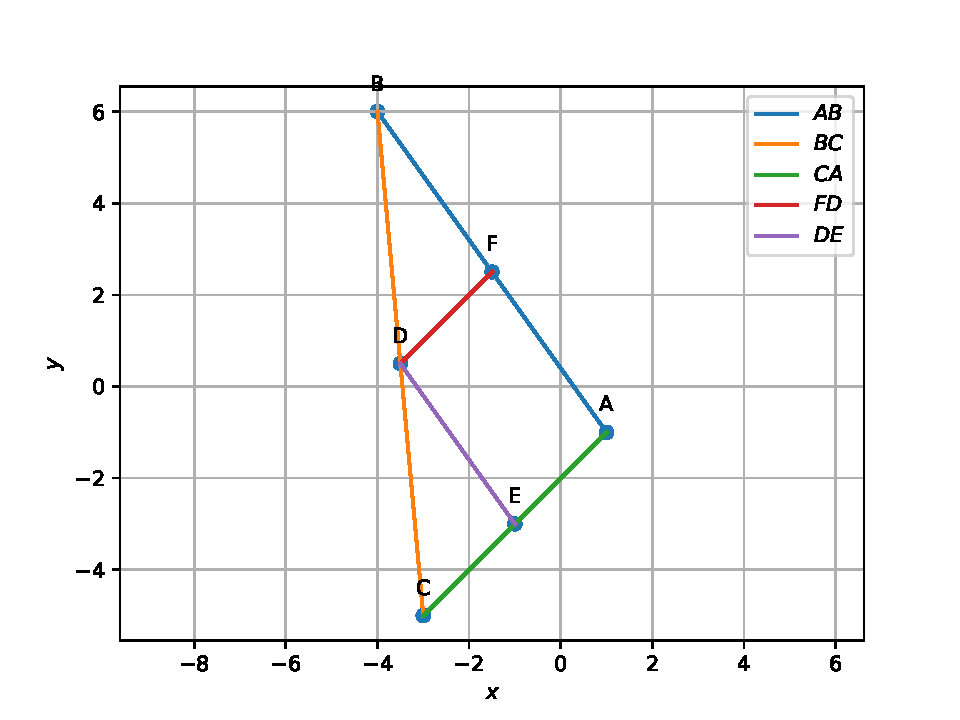
\includegraphics[width=0.75\columnwidth]{figs/triangle/pgm.pdf}
\caption{$AFDE$ forms a parallelogram in triangle ABC}
\label{fig:Triangle-pgm}
\end{figure}






















\item   Points $\vec{A}, \vec{B}, \vec{C}$ are defined to be collinear if 
		\begin{align}
			\label{eq:app-app-line-rank}
			\rank{\myvec{1 & 1 & 1 \\ \vec{A}& \vec{B}&\vec{C}}} = 2
		\end{align}
Are the given points in
			\eqref{eq:app-tri-pts}
collinear?
\\
\solution 
From 
			\eqref{eq:app-tri-pts},
\begin{align}
    \label{eq:app-1.1.3,2}
\myvec{
    1 & 1 & 1\\
    \vec{A} & \vec{B} & \vec{C} \\
    } 
    =
    %\label{eq:app-matthrowoperations}
    \myvec{
    1 & 1 & 1
    \\
    1 & -4 & -3
    \\
    -1 & 6 & -5
    }
     \xleftrightarrow[]{R_3 \leftarrow R_3+R_2}
    \myvec{
    1 & 1 & 1
    \\
    1 & -4 & -3
    \\
    0 & 2 & -8 
    }
    \\
     \xleftrightarrow[]{R_2\leftarrow R_1-R_2}
    \myvec{
    1 & 1 & 1
    \\
    0 & 5 & 4
    \\
    0 & 2 & -8 
    }
     \xleftrightarrow[]{R_3\leftarrow R_3-\frac{2}{5}R_2}
    \myvec{
    1 & 1 & 1
    \\
    0 & 5 & 4
    \\
    0 & 0 & \frac{-48}{5}
    }
\end{align}
There are no zero rows. So,
\begin{align}
    \text{rank}\myvec{
    1 & 1 & 1\\
    \vec{A} & \vec{B} & \vec{C} \\
    } &= 3 
\end{align}  
Hence,  the points $\vec{A},\vec{B},\vec{C}$ are not collinear. 
This is visible in 
\figref{fig1:Triangle}.
\begin{figure}[H]
\centering
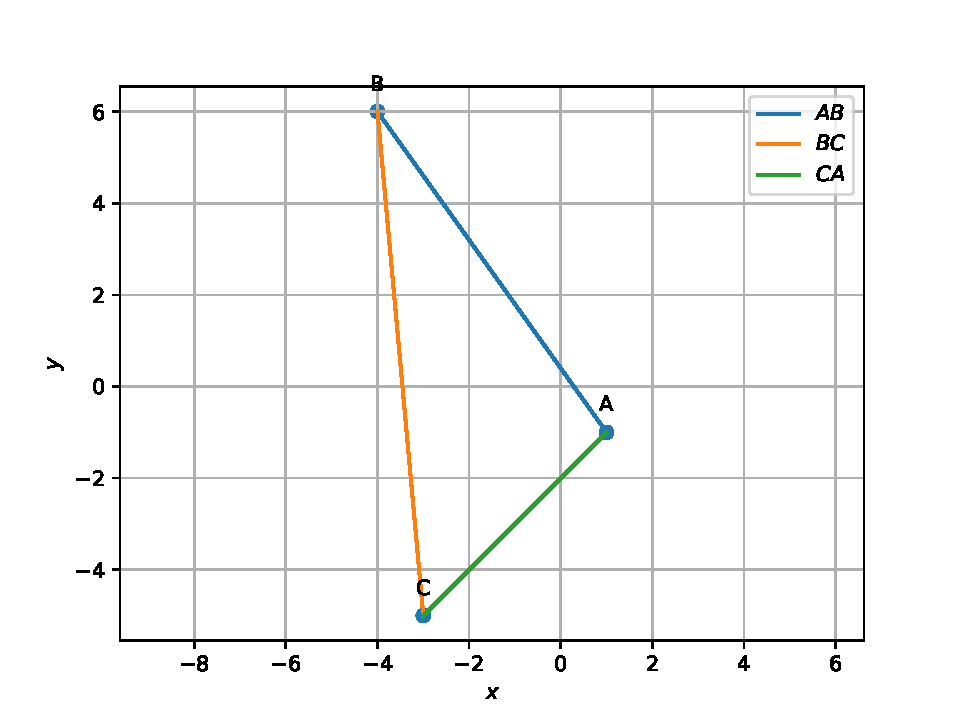
\includegraphics[width=0.75\columnwidth]{figs/triangle/vector.pdf}
\caption{$\triangle ABC$}
\label{fig1:Triangle}
\end{figure}
% \\		\\ \solution 
\begin{align}
    \vec{A}-\vec{F}&=\myvec{1\\-1}-\myvec{\frac{-3}{2}\\\frac{5}{2}}
    =\myvec{\frac{5}{2}\\\frac{-7}{2}}
    \\
    \vec{E}-\vec{D}&=\myvec{-1\\-3}-\myvec{\frac{-7}{2}\\\frac{1}{2}}
    =\myvec{\frac{5}{2}\\\frac{-7}{2}}
    \\
	\implies	\vec{A}-\vec{F} &= \vec{E}-\vec{D}
\end{align}
See \figref{fig:Triangle-pgm}, 
\begin{figure}
\centering
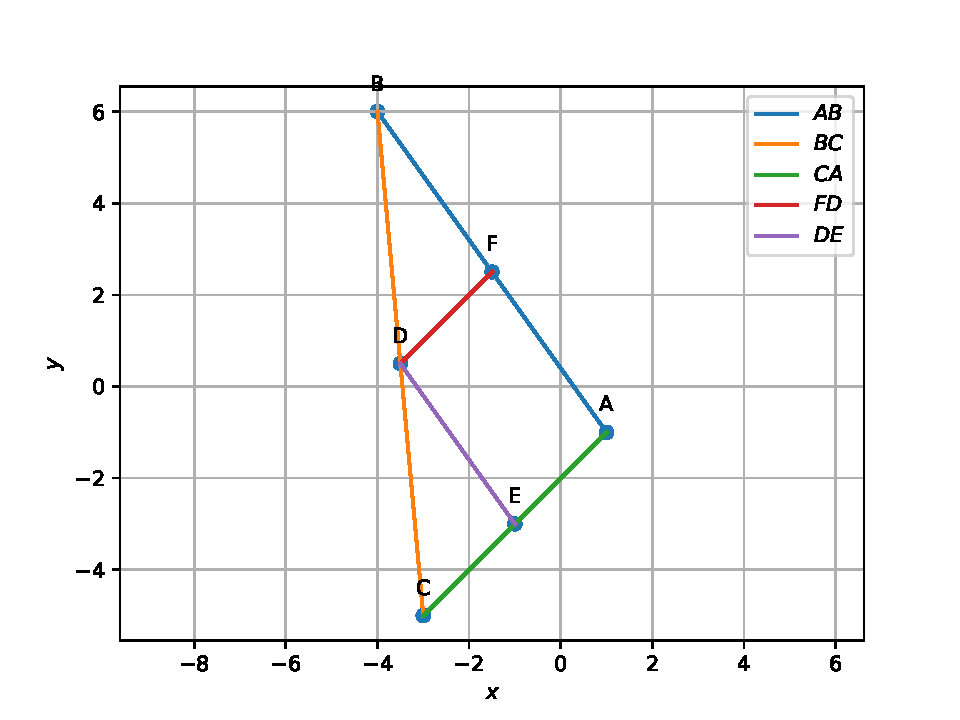
\includegraphics[width=0.75\columnwidth]{figs/triangle/pgm.pdf}
\caption{$AFDE$ forms a parallelogram in triangle ABC}
\label{fig:Triangle-pgm}
\end{figure}






















\item The parameteric form of the equation  of $AB$ is 
		\begin{align}
			\label{eq:app-geo-param}
			\vec{x}=\vec{A}+k\vec{m} \quad k \ne 0,
		\end{align}
		where
		\begin{align}
\vec{m}=\vec{B}-\vec{A}
		\end{align}
is the direction vector of $AB$.
Find the parameteric equations of $AB, BC$ and $CA$.
\\
\solution
From 
			\eqref{eq:app-geo-param} and
		\eqref{eq:app-geo-dir-vec-ab},
the parametric equation for $AB$ is given by
\begin{align}
AB: \vec{x} = &\myvec{1\\-1} + k \myvec{-5\\7}
\end{align}
Similarly, from 
		\eqref{eq:app-geo-dir-vec-bc} and
		\eqref{eq:app-geo-dir-vec-ca},
\begin{align}
BC: \vec{x} = &\myvec{-4\\6} + k \myvec{1\\-11}\\
CA: \vec{x} = &\myvec{-3\\-5} + k \myvec{4\\4}
\end{align}

%		\\ \solution 
\begin{align}
    \vec{A}-\vec{F}&=\myvec{1\\-1}-\myvec{\frac{-3}{2}\\\frac{5}{2}}
    =\myvec{\frac{5}{2}\\\frac{-7}{2}}
    \\
    \vec{E}-\vec{D}&=\myvec{-1\\-3}-\myvec{\frac{-7}{2}\\\frac{1}{2}}
    =\myvec{\frac{5}{2}\\\frac{-7}{2}}
    \\
	\implies	\vec{A}-\vec{F} &= \vec{E}-\vec{D}
\end{align}
See \figref{fig:Triangle-pgm}, 
\begin{figure}
\centering
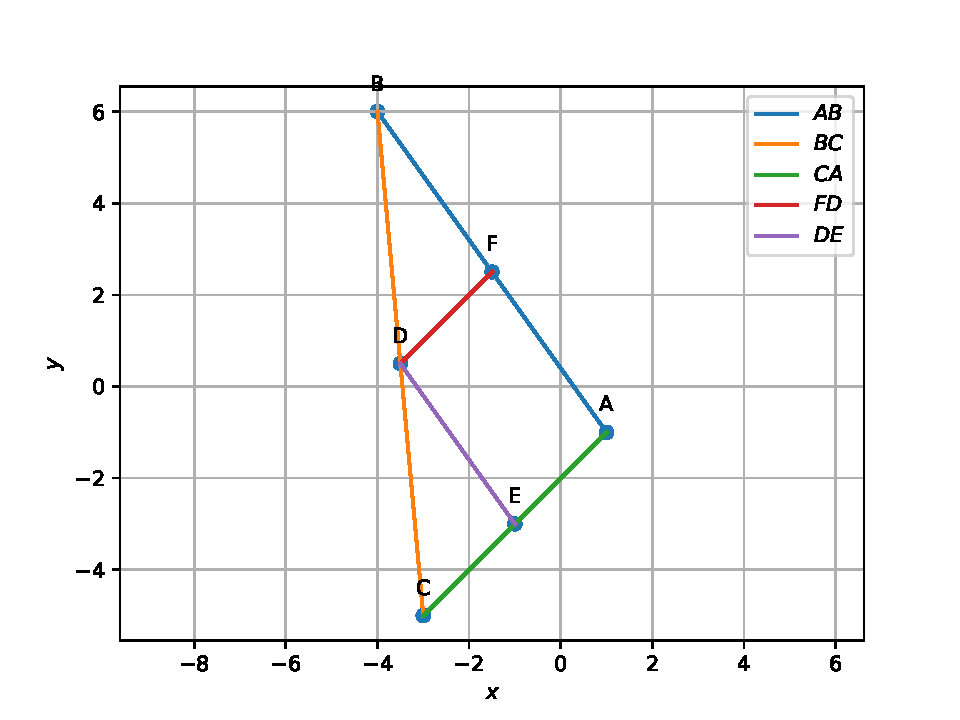
\includegraphics[width=0.75\columnwidth]{figs/triangle/pgm.pdf}
\caption{$AFDE$ forms a parallelogram in triangle ABC}
\label{fig:Triangle-pgm}
\end{figure}






















\item The normal form of the equation of $AB$  is 
		\begin{align}
			\label{eq:app-geo-normal}
			\vec{n}^{\top}\brak{	\vec{x}-\vec{A}} = 0
		\end{align}
		where 
		\begin{align}
			\vec{n}^{\top}\vec{m}&=\vec{n}^{\top}\brak{\vec{B}-\vec{A}} = 0
			\\
			\text{or, } \vec{n}&=\myvec{0 & 1 \\ -1 & 0} \vec{m}
			\label{eq:app-geo-norm-vec}
		\end{align}
Find the normal form of the equations of $AB, BC$ and $CA$.
\\
\solution
\begin{enumerate}
	\item
From
		\eqref{eq:app-geo-dir-vec-bc}, 
the direction vector of side $\vec{BC}$ is
\begin{align}
\vec{m}
	&=\myvec{1\\-11}
	\\
\implies \vec{n} &= \myvec{0 & 1\\
  -1 & 0}\myvec{1\\-11}
 = \myvec{-11\\-1}
		\label{eq:app-geo-norm-vec-bc}
\end{align}
from 
			\eqref{eq:app-geo-norm-vec}.
Hence, from 
			\eqref{eq:app-geo-normal},
the normal equation of side $BC$ is 
\begin{align}
	\vec{n}^{\top}\brak{	\vec{x}-\vec{B}} &= 0
			\\
\implies    \myvec{-11 & -1}\vec{x}&=\myvec{-11 & -1}\myvec{-4\\6}\\
    \implies
BC: \quad    \myvec{11 & 1}\vec{x}&=-38
\end{align}
\item Similarly, for $AB$,
from 
		\eqref{eq:app-geo-dir-vec-ab}, 
\begin{align}
	\vec{m} &= \myvec{-5\\7}
	\\
\implies        \vec{n} 
                &= \myvec{0&1\\-1&0}\myvec{-5\\7}
                = \myvec{7\\5}
		\label{eq:app-geo-norm-vec-ab}
\end{align}
and 
\begin{align}
	\vec{n}^{\top}\brak{	\vec{x}-\vec{A}} &= 0
	\\
	\implies
                AB: \quad  \vec{n}^{\top}\vec{x} &= \myvec{7&5}\myvec{1\\-1}\\    
       \implies\myvec{7&5}\vec{x} &= 2
\end{align}
\item For 
$CA$, 
from 
		\eqref{eq:app-geo-dir-vec-ca}, 
\begin{align}
\vec{m} &= \myvec{1 \\ 1}
\\
		\label{eq:app-geo-norm-vec-ca}
\implies \vec{n} 
&= \myvec{0&1 \\ -1&0}\myvec{1 \\ 1}
= \myvec{1 \\ -1}\\
\\
\implies	\vec{n}^{\top}\brak{	\vec{x}-\vec{C}} &= 0
\\
\implies \myvec{1&-1}{\vec{x}} &= \myvec{1&-1}\myvec{-3 \\ -5} 
= 2 
\end{align}
\end{enumerate}

%\begin{enumerate}
	\item
From
		\eqref{eq:geo-dir-vec-bc}, 
the direction vector of side $\vec{BC}$ is
\begin{align}
\vec{m}
	&=\myvec{1\\-11}
	\\
\implies \vec{n} &= \myvec{0 & 1\\
  -1 & 0}\myvec{1\\-11}
 = \myvec{-11\\-1}
		\label{eq:geo-norm-vec-bc}
\end{align}
from 
			\eqref{eq:geo-norm-vec}.
Hence, from 
			\eqref{eq:geo-normal},
the normal equation of side $BC$ is 
\begin{align}
	\vec{n}^{\top}\brak{	\vec{x}-\vec{B}} &= 0
			\\
\implies    \myvec{-11 & -1}\vec{x}&=\myvec{-11 & -1}\myvec{-4\\6}\\
    \implies
BC: \quad    \myvec{11 & 1}\vec{x}&=-38
\end{align}
\item Similarly, for $AB$,
from 
		\eqref{eq:geo-dir-vec-ab}, 
\begin{align}
	\vec{m} &= \myvec{-5\\7}
	\\
\implies        \vec{n} 
                &= \myvec{0&1\\-1&0}\myvec{-5\\7}
                = \myvec{7\\5}
		\label{eq:geo-norm-vec-ab}
\end{align}
and 
\begin{align}
	\vec{n}^{\top}\brak{	\vec{x}-\vec{A}} &= 0
	\\
	\implies
                AB: \quad  \vec{n}^{\top}\vec{x} &= \myvec{7&5}\myvec{1\\-1}\\    
       \implies\myvec{7&5}\vec{x} &= 2
\end{align}
\item For 
$CA$, 
from 
		\eqref{eq:geo-dir-vec-ca}, 
\begin{align}
\vec{m} &= \myvec{1 \\ 1}
\\
		\label{eq:geo-norm-vec-ca}
\implies \vec{n} 
&= \myvec{0&1 \\ -1&0}\myvec{1 \\ 1}
= \myvec{1 \\ -1}\\
\\
\implies	\vec{n}^{\top}\brak{	\vec{x}-\vec{C}} &= 0
\\
\implies \myvec{1&-1}{\vec{x}} &= \myvec{1&-1}\myvec{-3 \\ -5} 
= 2 
\end{align}
\end{enumerate}


\item The area of $\triangle ABC$ is defined as
		\begin{align}
			\label{eq:app-tri-area-cross}
			\frac{1}{2}\norm{{\brak{\vec{A}-\vec{B}}\times \brak{\vec{A}-\vec{C}}}}
		\end{align}
		where
		\begin{align}
			\vec{A}\times\vec{B} \triangleq \mydet{1 & -4 \\-1 & 6}
		\end{align}
		Find the area of $\triangle ABC$.\\
\solution
From
		\eqref{eq:app-geo-dir-vec-ab}
		and
		\eqref{eq:app-geo-dir-vec-ca},
\begin{align}
	\vec{A}-\vec{B}=\myvec{5\\-7},
	\vec{A}-\vec{C}&=\myvec{4\\4}\\
\implies (\vec{A}-\vec{B})\times(\vec{A}-\vec{C}) &=\mydet{5 & 4\\-7 & 4}\\
&=5\times 4-4\times (-7)\\&=48\\
\implies\frac{1}{2}\norm{(\vec{A}-\vec{B})\times(\vec{A}-\vec{C})}&=\frac{48}{2}=24
\end{align}
which is the desired area.

%  		\\ \solution 
\begin{align}
    \vec{A}-\vec{F}&=\myvec{1\\-1}-\myvec{\frac{-3}{2}\\\frac{5}{2}}
    =\myvec{\frac{5}{2}\\\frac{-7}{2}}
    \\
    \vec{E}-\vec{D}&=\myvec{-1\\-3}-\myvec{\frac{-7}{2}\\\frac{1}{2}}
    =\myvec{\frac{5}{2}\\\frac{-7}{2}}
    \\
	\implies	\vec{A}-\vec{F} &= \vec{E}-\vec{D}
\end{align}
See \figref{fig:Triangle-pgm}, 
\begin{figure}
\centering
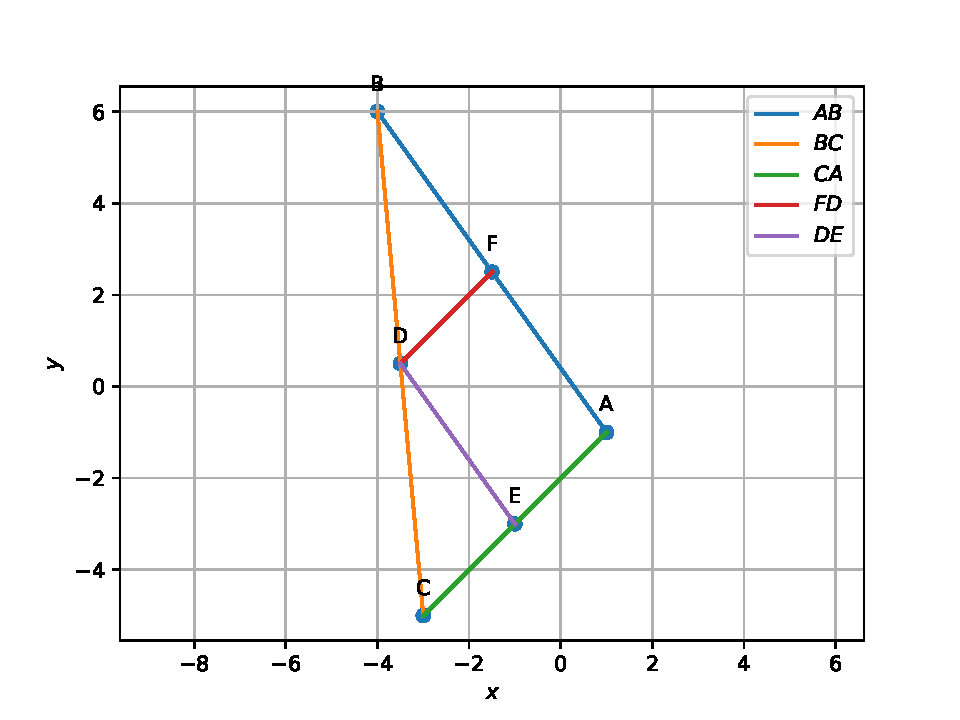
\includegraphics[width=0.75\columnwidth]{figs/triangle/pgm.pdf}
\caption{$AFDE$ forms a parallelogram in triangle ABC}
\label{fig:Triangle-pgm}
\end{figure}






















	\item Find the angles $A, B, C$ if 
%    \label{prop:angle2d}
  \begin{align}
    \label{eq:app-angle2d}
			\cos A \triangleq 
\frac{\brak{\vec{B}-\vec{A}}^{\top}{\vec{C}-\vec{A}}}{\norm{\vec{B}-\vec{A}}\norm{\vec{C}-\vec{A}}}
  \end{align}\\
  \solution
\begin{enumerate}
	\item From 
		\eqref{eq:app-geo-dir-vec-ab},
		\eqref{eq:app-geo-dir-vec-ca},
		\eqref{eq:app-geo-norm-ab}
		and
		\eqref{eq:app-geo-norm-ca}
\begin{align}
	(\vec{B}-\vec{A})^{\top}(\vec{C}-\vec{A})&=\myvec{-5&7}\myvec{-4\\-4}\\
	&=-8
	\\
	\implies
	\cos{A}&= \frac{-8}{\sqrt{74} \sqrt{32}}
	= \frac{-1}{\sqrt{37}}\\
	\implies A&=\cos^{-1}{\frac{-1}{\sqrt{37}}}
\end{align}
	\item From 
		\eqref{eq:app-geo-dir-vec-ab},
		\eqref{eq:app-geo-dir-vec-bc},
		\eqref{eq:app-geo-norm-ab}
		and
		\eqref{eq:app-geo-norm-bc}
\begin{align}
	(\vec{C}-\vec{B})^{\top}(\vec{A}-\vec{B})&=\myvec{1&-11}\myvec{5\\-7}\\
	&= 82
	\\
	\implies
	\cos{B}&= \frac{82}{\sqrt{74} \sqrt{122}}
	= \frac{41}{\sqrt{2257}}\\
	\implies B&=\cos^{-1}{\frac{41}{\sqrt{2257}}}
\end{align}
	\item From 
		\eqref{eq:app-geo-dir-vec-bc},
		\eqref{eq:app-geo-dir-vec-ca},
		\eqref{eq:app-geo-norm-bc}
		and
		\eqref{eq:app-geo-norm-ca}
\begin{align}
	(\vec{A}-\vec{C})^{\top}(\vec{B}-\vec{C})&=\myvec{4&4}\myvec{-1\\11}\\
	&=40
	\\
\implies	\cos{C}&= \frac{40}{\sqrt{32} \sqrt{122}}
	= \frac{5}{\sqrt{61}}\\
	\implies C&=\cos^{-1}{\frac{5}{\sqrt{61}}}
\end{align}

\end{enumerate}
%  	\\ \solution 
\begin{align}
    \vec{A}-\vec{F}&=\myvec{1\\-1}-\myvec{\frac{-3}{2}\\\frac{5}{2}}
    =\myvec{\frac{5}{2}\\\frac{-7}{2}}
    \\
    \vec{E}-\vec{D}&=\myvec{-1\\-3}-\myvec{\frac{-7}{2}\\\frac{1}{2}}
    =\myvec{\frac{5}{2}\\\frac{-7}{2}}
    \\
	\implies	\vec{A}-\vec{F} &= \vec{E}-\vec{D}
\end{align}
See \figref{fig:Triangle-pgm}, 
\begin{figure}
\centering
\includegraphics[width=0.75\columnwidth]{figs/triangle/pgm.pdf}
\caption{$AFDE$ forms a parallelogram in triangle ABC}
\label{fig:Triangle-pgm}
\end{figure}






















All codes for this section are available at
\begin{lstlisting}
	codes/triangle/sides.py
\end{lstlisting}
\end{enumerate}

\item Find the point on the X axis which is equidistant from $(2, -5)$ and $(-2, 9)$.
	\label{it:10/7/1/7}
	\\
\solution
		%\renewcommand{\theequation}{\theenumi}
\begin{enumerate}[label=\thesubsection.\arabic*.,ref=\thesubsection.\theenumi]
%\numberwithin{equation}{enumi}
\item The direction vector of $AB$ is defined as
		\begin{align}
			\vec{B}-
			\vec{A}
		\end{align}
Find the direction vectors of $AB, BC$ and $CA$.
\\
\solution 
\begin{enumerate} 
\item  The Direction vector of $AB$ is 
	\begin{align}  \vec{B} - \vec{A} 
		=\myvec{ -4\\ 6 } - \myvec{ 1\\ -1 }
 = \myvec{ -4 - 1\\ 6 - (-1) } = \myvec{ -5\\ 7 }
		\label{eq:app-geo-dir-vec-ab}
 \end{align}
\item The Direction vector of $BC$ is
	\begin{align} \vec{C} - \vec{B}=\myvec{ -3\\ -5} - \myvec{ -4\\ 6 }
 = \myvec{ -3 - (-4)\\ -5 - 6 } = \myvec{1\\ -11 }
		\label{eq:app-geo-dir-vec-bc}
  \end{align}
  \item  The Direction vector of $CA$  is
	  \begin{align}  \vec{A} - \vec{C} =\myvec{ 1\\ -1 }-\myvec{ -3\\ -5}
 = \myvec{ 1 - (-3)\\ -1 - (-5) } = \myvec{ 4\\ 4 }
		\label{eq:app-geo-dir-vec-ca}
  \end{align}
 \end{enumerate}
%	\solution 
\begin{enumerate} 
\item  The Direction vector of $AB$ is 
	\begin{align}  \vec{B} - \vec{A} 
		=\myvec{ -4\\ 6 } - \myvec{ 1\\ -1 }
 = \myvec{ -4 - 1\\ 6 - (-1) } = \myvec{ -5\\ 7 }
		\label{eq:geo-dir-vec-ab}
 \end{align}
\item The Direction vector of $BC$ is
	\begin{align} \vec{C} - \vec{B}=\myvec{ -3\\ -5} - \myvec{ -4\\ 6 }
 = \myvec{ -3 - (-4)\\ -5 - 6 } = \myvec{1\\ -11 }
		\label{eq:geo-dir-vec-bc}
  \end{align}
  \item  The Direction vector of $CA$  is
	  \begin{align}  \vec{A} - \vec{C} =\myvec{ 1\\ -1 }-\myvec{ -3\\ -5}
 = \myvec{ 1 - (-3)\\ -1 - (-5) } = \myvec{ 4\\ 4 }
		\label{eq:geo-dir-vec-ca}
  \end{align}
 \end{enumerate}


	\item The length of side $BC$ is 
		\label{prob:side-length}
		\begin{align}
			c = \norm{\vec{B}-\vec{A}} \triangleq \sqrt{\brak{\vec{B}-\vec{A}}^{\top}\brak{\vec{B}-\vec{A}}}
		\end{align}
		where
		\begin{align}
			\vec{A}^{\top}\triangleq\myvec{1 & -1}
		\end{align}
		Similarly, 
		\begin{align}
b = \norm{\vec{C}-\vec{B}},\,
a = \norm{\vec{A}-\vec{C}}
		\end{align}
		Find $a, b, c$.
\begin{enumerate}
	\item 
	From 	
		\eqref{eq:app-geo-dir-vec-ab},
\begin{align}
\vec{A}-\vec{B} &= \myvec{5\\-7}, \\
\implies 	c &= 	\norm{\vec{B}-\vec{A}} = \norm{\vec{A}-\vec{B}} 
	\\
	&= \sqrt{\myvec{5 & -7}\myvec{5\\-7}}
= \sqrt{\brak{5}^2 +\brak{7}^2}\\
	&=\sqrt{74}
		\label{eq:app-geo-norm-ab}
\end{align}
	\item Similarly, from 
		\eqref{eq:app-geo-dir-vec-bc},
\begin{align}
	a &= \norm{\vec{B}-\vec{C}} 
	= \sqrt{\myvec{-1 & 11}\myvec{-1\\11}}
\\
&= \sqrt{\brak{1}^2+\brak{11}^2}
	= \sqrt{122}
		\label{eq:app-geo-norm-bc}
\end{align}
and
		from 		\eqref{eq:app-geo-dir-vec-ca},
	\item 
		\begin{align}
			b &= \norm{\vec{A}-\vec{C}} = \sqrt{\myvec{4 & 4}\myvec{4\\4}}
\\
&= \sqrt{\brak{4}^2+\brak{4}^2}
	=\sqrt{32}
		\label{eq:app-geo-norm-ca}
\end{align}
\end{enumerate}
%  \\            
  %\\ \solution 
\begin{align}
    \vec{A}-\vec{F}&=\myvec{1\\-1}-\myvec{\frac{-3}{2}\\\frac{5}{2}}
    =\myvec{\frac{5}{2}\\\frac{-7}{2}}
    \\
    \vec{E}-\vec{D}&=\myvec{-1\\-3}-\myvec{\frac{-7}{2}\\\frac{1}{2}}
    =\myvec{\frac{5}{2}\\\frac{-7}{2}}
    \\
	\implies	\vec{A}-\vec{F} &= \vec{E}-\vec{D}
\end{align}
See \figref{fig:Triangle-pgm}, 
\begin{figure}
\centering
\includegraphics[width=0.75\columnwidth]{figs/triangle/pgm.pdf}
\caption{$AFDE$ forms a parallelogram in triangle ABC}
\label{fig:Triangle-pgm}
\end{figure}






















\item   Points $\vec{A}, \vec{B}, \vec{C}$ are defined to be collinear if 
		\begin{align}
			\label{eq:app-app-line-rank}
			\rank{\myvec{1 & 1 & 1 \\ \vec{A}& \vec{B}&\vec{C}}} = 2
		\end{align}
Are the given points in
			\eqref{eq:app-tri-pts}
collinear?
\\
\solution 
From 
			\eqref{eq:app-tri-pts},
\begin{align}
    \label{eq:app-1.1.3,2}
\myvec{
    1 & 1 & 1\\
    \vec{A} & \vec{B} & \vec{C} \\
    } 
    =
    %\label{eq:app-matthrowoperations}
    \myvec{
    1 & 1 & 1
    \\
    1 & -4 & -3
    \\
    -1 & 6 & -5
    }
     \xleftrightarrow[]{R_3 \leftarrow R_3+R_2}
    \myvec{
    1 & 1 & 1
    \\
    1 & -4 & -3
    \\
    0 & 2 & -8 
    }
    \\
     \xleftrightarrow[]{R_2\leftarrow R_1-R_2}
    \myvec{
    1 & 1 & 1
    \\
    0 & 5 & 4
    \\
    0 & 2 & -8 
    }
     \xleftrightarrow[]{R_3\leftarrow R_3-\frac{2}{5}R_2}
    \myvec{
    1 & 1 & 1
    \\
    0 & 5 & 4
    \\
    0 & 0 & \frac{-48}{5}
    }
\end{align}
There are no zero rows. So,
\begin{align}
    \text{rank}\myvec{
    1 & 1 & 1\\
    \vec{A} & \vec{B} & \vec{C} \\
    } &= 3 
\end{align}  
Hence,  the points $\vec{A},\vec{B},\vec{C}$ are not collinear. 
This is visible in 
\figref{fig1:Triangle}.
\begin{figure}[H]
\centering
\includegraphics[width=0.75\columnwidth]{figs/triangle/vector.pdf}
\caption{$\triangle ABC$}
\label{fig1:Triangle}
\end{figure}
% \\		\\ \solution 
\begin{align}
    \vec{A}-\vec{F}&=\myvec{1\\-1}-\myvec{\frac{-3}{2}\\\frac{5}{2}}
    =\myvec{\frac{5}{2}\\\frac{-7}{2}}
    \\
    \vec{E}-\vec{D}&=\myvec{-1\\-3}-\myvec{\frac{-7}{2}\\\frac{1}{2}}
    =\myvec{\frac{5}{2}\\\frac{-7}{2}}
    \\
	\implies	\vec{A}-\vec{F} &= \vec{E}-\vec{D}
\end{align}
See \figref{fig:Triangle-pgm}, 
\begin{figure}
\centering
\includegraphics[width=0.75\columnwidth]{figs/triangle/pgm.pdf}
\caption{$AFDE$ forms a parallelogram in triangle ABC}
\label{fig:Triangle-pgm}
\end{figure}






















\item The parameteric form of the equation  of $AB$ is 
		\begin{align}
			\label{eq:app-geo-param}
			\vec{x}=\vec{A}+k\vec{m} \quad k \ne 0,
		\end{align}
		where
		\begin{align}
\vec{m}=\vec{B}-\vec{A}
		\end{align}
is the direction vector of $AB$.
Find the parameteric equations of $AB, BC$ and $CA$.
\\
\solution
From 
			\eqref{eq:app-geo-param} and
		\eqref{eq:app-geo-dir-vec-ab},
the parametric equation for $AB$ is given by
\begin{align}
AB: \vec{x} = &\myvec{1\\-1} + k \myvec{-5\\7}
\end{align}
Similarly, from 
		\eqref{eq:app-geo-dir-vec-bc} and
		\eqref{eq:app-geo-dir-vec-ca},
\begin{align}
BC: \vec{x} = &\myvec{-4\\6} + k \myvec{1\\-11}\\
CA: \vec{x} = &\myvec{-3\\-5} + k \myvec{4\\4}
\end{align}

%		\\ \solution 
\begin{align}
    \vec{A}-\vec{F}&=\myvec{1\\-1}-\myvec{\frac{-3}{2}\\\frac{5}{2}}
    =\myvec{\frac{5}{2}\\\frac{-7}{2}}
    \\
    \vec{E}-\vec{D}&=\myvec{-1\\-3}-\myvec{\frac{-7}{2}\\\frac{1}{2}}
    =\myvec{\frac{5}{2}\\\frac{-7}{2}}
    \\
	\implies	\vec{A}-\vec{F} &= \vec{E}-\vec{D}
\end{align}
See \figref{fig:Triangle-pgm}, 
\begin{figure}
\centering
\includegraphics[width=0.75\columnwidth]{figs/triangle/pgm.pdf}
\caption{$AFDE$ forms a parallelogram in triangle ABC}
\label{fig:Triangle-pgm}
\end{figure}






















\item The normal form of the equation of $AB$  is 
		\begin{align}
			\label{eq:app-geo-normal}
			\vec{n}^{\top}\brak{	\vec{x}-\vec{A}} = 0
		\end{align}
		where 
		\begin{align}
			\vec{n}^{\top}\vec{m}&=\vec{n}^{\top}\brak{\vec{B}-\vec{A}} = 0
			\\
			\text{or, } \vec{n}&=\myvec{0 & 1 \\ -1 & 0} \vec{m}
			\label{eq:app-geo-norm-vec}
		\end{align}
Find the normal form of the equations of $AB, BC$ and $CA$.
\\
\solution
\begin{enumerate}
	\item
From
		\eqref{eq:app-geo-dir-vec-bc}, 
the direction vector of side $\vec{BC}$ is
\begin{align}
\vec{m}
	&=\myvec{1\\-11}
	\\
\implies \vec{n} &= \myvec{0 & 1\\
  -1 & 0}\myvec{1\\-11}
 = \myvec{-11\\-1}
		\label{eq:app-geo-norm-vec-bc}
\end{align}
from 
			\eqref{eq:app-geo-norm-vec}.
Hence, from 
			\eqref{eq:app-geo-normal},
the normal equation of side $BC$ is 
\begin{align}
	\vec{n}^{\top}\brak{	\vec{x}-\vec{B}} &= 0
			\\
\implies    \myvec{-11 & -1}\vec{x}&=\myvec{-11 & -1}\myvec{-4\\6}\\
    \implies
BC: \quad    \myvec{11 & 1}\vec{x}&=-38
\end{align}
\item Similarly, for $AB$,
from 
		\eqref{eq:app-geo-dir-vec-ab}, 
\begin{align}
	\vec{m} &= \myvec{-5\\7}
	\\
\implies        \vec{n} 
                &= \myvec{0&1\\-1&0}\myvec{-5\\7}
                = \myvec{7\\5}
		\label{eq:app-geo-norm-vec-ab}
\end{align}
and 
\begin{align}
	\vec{n}^{\top}\brak{	\vec{x}-\vec{A}} &= 0
	\\
	\implies
                AB: \quad  \vec{n}^{\top}\vec{x} &= \myvec{7&5}\myvec{1\\-1}\\    
       \implies\myvec{7&5}\vec{x} &= 2
\end{align}
\item For 
$CA$, 
from 
		\eqref{eq:app-geo-dir-vec-ca}, 
\begin{align}
\vec{m} &= \myvec{1 \\ 1}
\\
		\label{eq:app-geo-norm-vec-ca}
\implies \vec{n} 
&= \myvec{0&1 \\ -1&0}\myvec{1 \\ 1}
= \myvec{1 \\ -1}\\
\\
\implies	\vec{n}^{\top}\brak{	\vec{x}-\vec{C}} &= 0
\\
\implies \myvec{1&-1}{\vec{x}} &= \myvec{1&-1}\myvec{-3 \\ -5} 
= 2 
\end{align}
\end{enumerate}

%\begin{enumerate}
	\item
From
		\eqref{eq:geo-dir-vec-bc}, 
the direction vector of side $\vec{BC}$ is
\begin{align}
\vec{m}
	&=\myvec{1\\-11}
	\\
\implies \vec{n} &= \myvec{0 & 1\\
  -1 & 0}\myvec{1\\-11}
 = \myvec{-11\\-1}
		\label{eq:geo-norm-vec-bc}
\end{align}
from 
			\eqref{eq:geo-norm-vec}.
Hence, from 
			\eqref{eq:geo-normal},
the normal equation of side $BC$ is 
\begin{align}
	\vec{n}^{\top}\brak{	\vec{x}-\vec{B}} &= 0
			\\
\implies    \myvec{-11 & -1}\vec{x}&=\myvec{-11 & -1}\myvec{-4\\6}\\
    \implies
BC: \quad    \myvec{11 & 1}\vec{x}&=-38
\end{align}
\item Similarly, for $AB$,
from 
		\eqref{eq:geo-dir-vec-ab}, 
\begin{align}
	\vec{m} &= \myvec{-5\\7}
	\\
\implies        \vec{n} 
                &= \myvec{0&1\\-1&0}\myvec{-5\\7}
                = \myvec{7\\5}
		\label{eq:geo-norm-vec-ab}
\end{align}
and 
\begin{align}
	\vec{n}^{\top}\brak{	\vec{x}-\vec{A}} &= 0
	\\
	\implies
                AB: \quad  \vec{n}^{\top}\vec{x} &= \myvec{7&5}\myvec{1\\-1}\\    
       \implies\myvec{7&5}\vec{x} &= 2
\end{align}
\item For 
$CA$, 
from 
		\eqref{eq:geo-dir-vec-ca}, 
\begin{align}
\vec{m} &= \myvec{1 \\ 1}
\\
		\label{eq:geo-norm-vec-ca}
\implies \vec{n} 
&= \myvec{0&1 \\ -1&0}\myvec{1 \\ 1}
= \myvec{1 \\ -1}\\
\\
\implies	\vec{n}^{\top}\brak{	\vec{x}-\vec{C}} &= 0
\\
\implies \myvec{1&-1}{\vec{x}} &= \myvec{1&-1}\myvec{-3 \\ -5} 
= 2 
\end{align}
\end{enumerate}


\item The area of $\triangle ABC$ is defined as
		\begin{align}
			\label{eq:app-tri-area-cross}
			\frac{1}{2}\norm{{\brak{\vec{A}-\vec{B}}\times \brak{\vec{A}-\vec{C}}}}
		\end{align}
		where
		\begin{align}
			\vec{A}\times\vec{B} \triangleq \mydet{1 & -4 \\-1 & 6}
		\end{align}
		Find the area of $\triangle ABC$.\\
\solution
From
		\eqref{eq:app-geo-dir-vec-ab}
		and
		\eqref{eq:app-geo-dir-vec-ca},
\begin{align}
	\vec{A}-\vec{B}=\myvec{5\\-7},
	\vec{A}-\vec{C}&=\myvec{4\\4}\\
\implies (\vec{A}-\vec{B})\times(\vec{A}-\vec{C}) &=\mydet{5 & 4\\-7 & 4}\\
&=5\times 4-4\times (-7)\\&=48\\
\implies\frac{1}{2}\norm{(\vec{A}-\vec{B})\times(\vec{A}-\vec{C})}&=\frac{48}{2}=24
\end{align}
which is the desired area.

%  		\\ \solution 
\begin{align}
    \vec{A}-\vec{F}&=\myvec{1\\-1}-\myvec{\frac{-3}{2}\\\frac{5}{2}}
    =\myvec{\frac{5}{2}\\\frac{-7}{2}}
    \\
    \vec{E}-\vec{D}&=\myvec{-1\\-3}-\myvec{\frac{-7}{2}\\\frac{1}{2}}
    =\myvec{\frac{5}{2}\\\frac{-7}{2}}
    \\
	\implies	\vec{A}-\vec{F} &= \vec{E}-\vec{D}
\end{align}
See \figref{fig:Triangle-pgm}, 
\begin{figure}
\centering
\includegraphics[width=0.75\columnwidth]{figs/triangle/pgm.pdf}
\caption{$AFDE$ forms a parallelogram in triangle ABC}
\label{fig:Triangle-pgm}
\end{figure}






















	\item Find the angles $A, B, C$ if 
%    \label{prop:angle2d}
  \begin{align}
    \label{eq:app-angle2d}
			\cos A \triangleq 
\frac{\brak{\vec{B}-\vec{A}}^{\top}{\vec{C}-\vec{A}}}{\norm{\vec{B}-\vec{A}}\norm{\vec{C}-\vec{A}}}
  \end{align}\\
  \solution
\begin{enumerate}
	\item From 
		\eqref{eq:app-geo-dir-vec-ab},
		\eqref{eq:app-geo-dir-vec-ca},
		\eqref{eq:app-geo-norm-ab}
		and
		\eqref{eq:app-geo-norm-ca}
\begin{align}
	(\vec{B}-\vec{A})^{\top}(\vec{C}-\vec{A})&=\myvec{-5&7}\myvec{-4\\-4}\\
	&=-8
	\\
	\implies
	\cos{A}&= \frac{-8}{\sqrt{74} \sqrt{32}}
	= \frac{-1}{\sqrt{37}}\\
	\implies A&=\cos^{-1}{\frac{-1}{\sqrt{37}}}
\end{align}
	\item From 
		\eqref{eq:app-geo-dir-vec-ab},
		\eqref{eq:app-geo-dir-vec-bc},
		\eqref{eq:app-geo-norm-ab}
		and
		\eqref{eq:app-geo-norm-bc}
\begin{align}
	(\vec{C}-\vec{B})^{\top}(\vec{A}-\vec{B})&=\myvec{1&-11}\myvec{5\\-7}\\
	&= 82
	\\
	\implies
	\cos{B}&= \frac{82}{\sqrt{74} \sqrt{122}}
	= \frac{41}{\sqrt{2257}}\\
	\implies B&=\cos^{-1}{\frac{41}{\sqrt{2257}}}
\end{align}
	\item From 
		\eqref{eq:app-geo-dir-vec-bc},
		\eqref{eq:app-geo-dir-vec-ca},
		\eqref{eq:app-geo-norm-bc}
		and
		\eqref{eq:app-geo-norm-ca}
\begin{align}
	(\vec{A}-\vec{C})^{\top}(\vec{B}-\vec{C})&=\myvec{4&4}\myvec{-1\\11}\\
	&=40
	\\
\implies	\cos{C}&= \frac{40}{\sqrt{32} \sqrt{122}}
	= \frac{5}{\sqrt{61}}\\
	\implies C&=\cos^{-1}{\frac{5}{\sqrt{61}}}
\end{align}

\end{enumerate}
%  	\\ \solution 
\begin{align}
    \vec{A}-\vec{F}&=\myvec{1\\-1}-\myvec{\frac{-3}{2}\\\frac{5}{2}}
    =\myvec{\frac{5}{2}\\\frac{-7}{2}}
    \\
    \vec{E}-\vec{D}&=\myvec{-1\\-3}-\myvec{\frac{-7}{2}\\\frac{1}{2}}
    =\myvec{\frac{5}{2}\\\frac{-7}{2}}
    \\
	\implies	\vec{A}-\vec{F} &= \vec{E}-\vec{D}
\end{align}
See \figref{fig:Triangle-pgm}, 
\begin{figure}
\centering
\includegraphics[width=0.75\columnwidth]{figs/triangle/pgm.pdf}
\caption{$AFDE$ forms a parallelogram in triangle ABC}
\label{fig:Triangle-pgm}
\end{figure}






















All codes for this section are available at
\begin{lstlisting}
	codes/triangle/sides.py
\end{lstlisting}
\end{enumerate}

\item Find the values of $y$ for which the distance between the points                  $\vec{P}(2, -3)$ and $\vec{Q}(10, y)$ is 10 units.
\item  If $\vec{Q}(0,  1)$ is equidistant from $\vec{P}(5,  -3)$ and $\vec{R}(x,  6)$,  find the values of $x$. Also find the
distances $QR$ and $PR$.
\item  Find a relation between $x$ and $y$ such that the point $(x, y)$ is equidistant from the point
$(3,  6)$ and $(– 3,  4)$.
	\item Find a point on the X axis, which is equidistant from the points $\myvec{
  7 \\
  6 \\
 }$ and $\myvec{
  3 \\
  4 \\
 }$
.
\label{chapters/11/10/1/4}
%	\\
%	\solution 
%The direction vector
\begin{align}
	\vec{B}-\vec{A}
	=
	\myvec{
  h-x_1\\
  k-y_1
  }
   \equiv
	\myvec{
1\\
	\frac{ k-y_1}{h-x_1}
  }
  \\
	\implies m = 
	\frac{ k-y_1}{h-x_1},
\end{align}
yielding the desired result.

\item The distance between the points $\vec{A}(0,  6) \text{ and } \vec{B}(0,  –2)$ is
\item The distance of the point $\vec{P} (–6,  8)$ from the origin is
\item The distance between the points $\vec(0,  5)\text{ and }(–5,  0)$ is
\item $AOBC$ is a rectangle whose three vertices are vertices $\vec{A} (0,  3),  \vec{O}(0,  0)\text{ and }
	\vec{B} (5,  0)$. The length of its diagonal is
\item The perimeter of a triangle with vertices $\vec(0,  4),  (0,  0) \text{ and } (3,  0)$ is
\item If the distance between the points $(4, P)$  and $ (1, 0)$ is 5, then the value of $P$ is
\item Find the points on the $X$ axis which are at a distance on $2\sqrt{5}$ from the point $ (7, -4).$ How many such points are there?
\item Find the value of $a$,  if the if the distance between the points $\vec{A}(-3, -14)$  and $\vec{B}(a, -5)$ is 9 units.
\item Find a point which is equidistant from the points $\vec{A}(-5, 4)$  and $(-1, 6)$.  How many such points are there ?
\item If the point $\vec{A}(2, -4)$ is equidistant from $\vec{P}(3, 8)$  and $\vec{Q}(-10, y)$,  find the values of $y$.  Also find distance $PQ$.
\item If $(a, b)$ is the mid-point of the line segment joining the point $\vec{A}(10, -6)\text{ and }\vec{B}(k, 4)$ and $a-2b=18$,  find the value of $a, b$ and the distance $AB$.
\item Find a relation between $x$ and $y$ such that the point $(x,y)$ is equidistant from the points $(7,1)$ and $(3,5)$.
\item Find a point on the Y axis which is equidistant from the points $\vec{A}(6,5)$ and $\vec{B}(-4,3)$.
\item Find the equation of set of points $\vec{P}$ such that $PA^2+PB^2=2k^2$, where $\vec{A}$ and $\vec{B}$ are the points $(3,4,5)$ and $(-1,3,-7)$, respectively.
\item Find the equation of the set of the points $\vec{P}$ such that its distances from the points $\vec{A}(3,4,-5)$ and $\vec{B}(-2,1,4)$ are equal.
\item Find a vector in the direction of vector $\overrightarrow{a}=\hat{i} -2\hat{j}$ that has magnitude $7$ units.
\end{enumerate}

\subsection{Unit Vector}
\begin{enumerate}[label=\thesubsection.\arabic*, ref=\thesubsection.\theenumi]
\item Find the value of $x$ for which $x(\hat{i}+\hat{j}+\hat{k})$ is a unit vector.\\
	\solution
		From the given information,
		\begin{align}
			\vec{a}=\myvec{\cos\frac{\pi}{3}\\\cos\frac{\pi}{4}\\\cos\theta}
			= 
\myvec{\frac{1}{2}\\[1ex]\frac{1}{\sqrt{2}}\\[1ex]\cos\theta}
		\end{align}
\begin{align}
\because    \norm{\vec{a}}&=1,
\\
\frac{1}{4}+\frac{1}{2}+\cos^2\theta&=1
\\
    \implies\cos\theta &=\frac{1}{2}
\end{align}
$\because \theta$ is an acute angle.
    Hence 
\begin{align}
		\vec{a}=\myvec{\frac{1}{2}\\[1ex] \frac{1}{\sqrt{2}}\\[1ex] \frac{1}{2}}
\end{align}

\item For given vectors,  $\vec{a}=2\hat{i}-\hat{j}+2\hat{k}$ and $\vec{b}=-\hat{i}+\hat{j}-\hat{k}$ ,  find the unit vector in the
direction of the vector $\vec{a}+\vec{b}$.
        \label{prob:12/10/2/9}
\\
    \solution 
		From the given information,
		\begin{align}
			\vec{a}=\myvec{\cos\frac{\pi}{3}\\\cos\frac{\pi}{4}\\\cos\theta}
			= 
\myvec{\frac{1}{2}\\[1ex]\frac{1}{\sqrt{2}}\\[1ex]\cos\theta}
		\end{align}
\begin{align}
\because    \norm{\vec{a}}&=1,
\\
\frac{1}{4}+\frac{1}{2}+\cos^2\theta&=1
\\
    \implies\cos\theta &=\frac{1}{2}
\end{align}
$\because \theta$ is an acute angle.
    Hence 
\begin{align}
		\vec{a}=\myvec{\frac{1}{2}\\[1ex] \frac{1}{\sqrt{2}}\\[1ex] \frac{1}{2}}
\end{align}

\item Find a vector in the direction of vector $5\hat{i}-\hat{j}+2\hat{k}$ which has magnitude 8 units.
        \label{prob:12/10/2/10const}
   \\ 
    \solution 
		From the given information,
		\begin{align}
			\vec{a}=\myvec{\cos\frac{\pi}{3}\\\cos\frac{\pi}{4}\\\cos\theta}
			= 
\myvec{\frac{1}{2}\\[1ex]\frac{1}{\sqrt{2}}\\[1ex]\cos\theta}
		\end{align}
\begin{align}
\because    \norm{\vec{a}}&=1,
\\
\frac{1}{4}+\frac{1}{2}+\cos^2\theta&=1
\\
    \implies\cos\theta &=\frac{1}{2}
\end{align}
$\because \theta$ is an acute angle.
    Hence 
\begin{align}
		\vec{a}=\myvec{\frac{1}{2}\\[1ex] \frac{1}{\sqrt{2}}\\[1ex] \frac{1}{2}}
\end{align}

\item Find the unit vector in the direction of sum of vectors $\vec{a}$= $2\hat{i}-\hat{j}+\hat{k}$  and  $\vec{b}=2\hat{j}+\hat{k}$.
\item If $\vec{a}$=$\hat{i}+\hat{j}+2\hat{k}$  and  $\vec{b}$=$2\hat{i}+\hat{j}-2\hat{k}$,  find the unit vector in the direction of
	\begin{enumerate}
		\item 6$\vec{a}$   
		\item 2$\vec{a}$-$\vec{b}$
	\end{enumerate}

\item Find a unit vector in the direction of $\overline{PQ} $,  where $\vec{P}$ and $\vec{Q}$ have co-ordinates (5, 0, 8) and (3, 3, 2), respectively.
\item The vector in the direction of the vector $\hat{i}-2\hat{j}+2\hat{k}$ that has magnitude 9 is
	\begin{enumerate}
\item $\hat{i}-2\hat{j}+2\hat{k}$
\item $\hat{i}-2\hat{j}$
\item $3(\hat{i}-2\hat{j}+2\hat{k})$
\item $9(\hat{i}-2\hat{j}+2\hat{k})$
\end{enumerate}
\item Find the unit vector in the direction of the vector $\vec{a}=\hat{i}+\hat{j}+2\hat{k}$.
\item Find the unit vector in the direction of vector $\overrightarrow{PQ}$ ,  where $\vec{P}$ and $\vec{Q}$ are the points
(1,  2,  3) and (4,  5,  6),  respectively.
\item Find a vector of magnitude 5 units,  and parallel to the resultant of the vectors $\vec{a}=2\hat{i}+3\hat{j}-\hat{k}$ and $\vec{b}=\hat{i}-2\hat{j}+\hat{k}$.\\
\item If $\vec{a}=\hat{i}+\hat{j}+\hat{k},  \vec{b}=2\hat{i}-\hat{j}+3\hat{k}$ and $\vec{c}=\hat{i}-2\hat{j}+\hat{k}$,  find a unit vector parallel to the vector $2\vec{a}-\vec{b}+3\vec{c}$.\\
	\solution
		From the given information,
		\begin{align}
			\vec{a}=\myvec{\cos\frac{\pi}{3}\\\cos\frac{\pi}{4}\\\cos\theta}
			= 
\myvec{\frac{1}{2}\\[1ex]\frac{1}{\sqrt{2}}\\[1ex]\cos\theta}
		\end{align}
\begin{align}
\because    \norm{\vec{a}}&=1,
\\
\frac{1}{4}+\frac{1}{2}+\cos^2\theta&=1
\\
    \implies\cos\theta &=\frac{1}{2}
\end{align}
$\because \theta$ is an acute angle.
    Hence 
\begin{align}
		\vec{a}=\myvec{\frac{1}{2}\\[1ex] \frac{1}{\sqrt{2}}\\[1ex] \frac{1}{2}}
\end{align}

	\item 
Find a vector of magnitude 5 units,  and parallel to the resultant of the vectors $\vec{a} = 2\hat{i}+3\hat{j}-\hat{k}$ and $\vec{b} = \hat{i}-2\hat{j}+\hat{k}$.
\\
\solution
		\begin{align}
\because     \Vec{a}=\myvec{
        2\\3\\-1
    },\Vec{b}=\myvec{
        1\\-2\\1
    }\\
	\vec{a}+\vec{b}=\myvec{
        3\\1\\0
    }
    \implies
	\norm{\vec{a}+\vec{b}}=\sqrt{10}
\end{align}
From problem
        \ref{prob:12/10/2/9},
the unit vector in the direction of 
${\vec{a}+\vec{b}}$
is
\begin{align}
	\frac{{\vec{a}+\vec{b}}}{\norm{\vec{a}+\vec{b}}}
=\frac{1}{\sqrt{10}}\myvec{
        3\\1\\0
    }
\end{align}
The desired vector can then be expressed as
\begin{align}
\pm\frac{5}{\sqrt{10}}\myvec{
        3\\1\\0
    }
\end{align}


	\item If a line makes angles $90\degree, 135\degree, 45\degree$ with X, Y and Z axis respectivly. Find its direction cosines.
		\\
		\solution
		\iffalse
\documentclass[10pt]{article}
\usepackage{graphicx}
\def\inputGnumericTable{}
\usepackage[latin1]{inputenc}
\usepackage{fullpage}
\usepackage{color}
\usepackage{array}
\usepackage{longtable}
\usepackage{calc}
\usepackage{multirow}
\usepackage{hhline}
\usepackage{ifthen}
\usepackage{amsmath}
\usepackage[none]{hyphenat}
\usepackage{listings}
\usepackage[english]{babel}
\usepackage{siunitx}
\usepackage{caption}
\usepackage{booktabs}
\usepackage{array}
\usepackage{extarrows}
\usepackage{enumerate}
\usepackage{enumitem}
\usepackage{amsmath}
\usepackage{commath}
\usepackage{gensymb}
\usepackage{amssymb}
\usepackage{multicol}
%\usepackage[utf8]{inputenc}
\lstset{
 frame=single,
 breaklines=true
}
\usepackage{hyperref}
\usepackage[margin=0.65in]{geometry}	 
%\usepackage{exsheets}% also loads the `tasks' package
\usepackage{atbegshi}
\AtBeginDocument{\AtBeginShipoutNext{\AtBeginShipoutDiscard}}

%new macro definitions
\renewcommand{\labelenumi}{(\roman{enumi})}
\newcommand{\mydet}[1]{\ensuremath{\begin{vmatrix}#1\end{vmatrix}}}
\providecommand{\brak}[1]{\ensuremath{\left(#1\right)}}
\newcommand{\solution}{\noindent \textbf{Solution: }}
\newcommand{\myvec}[1]{\ensuremath{\begin{pmatrix}#1\end{pmatrix}}}
\newenvironment{amatrix}[1]{%
	\left(\begin{array}{@{}*{#1}{c}|c@{}}
}{%
	\end{array}\right)
}

\newcommand{\myaugvec}[2]{\ensuremath{\begin{amatrix}{#1}#2\end{amatrix}}}
\providecommand{\norm}[1]{\left\1Vert#1\right\rVert}
\let\vec\mathbf{}


%\SetEnumitemKey{twocol}{
% before=\raggedcolumns\begin{multicols}{2},
% after=\end{multicols}}
%\SetEnumitemKey{fourcol}{
% before=\raggedcolumns\begin{multicols}{4},
% after=\end{multicols}} 


\begin{document}
\begin{center}
\title{\textbf{TRIANGLES}}
\date{\vspace{-5ex}}
\maketitle
\end{center}
\section*{9$^{th}$Math - Chapter 7}
This is Problem-8 from Exercise 7.1\\\\


\section*{\large Construction:}
\fi
The input parameters for construction
	are available in Table \ref{tab:chapters/9/7/1/8/table}.
\begin{table}[H]
	\centering
	%\subimport{../chapters/9/7/1/8/tables/}{table.tex}
     %%%%%%%%%%%%%%%%%%%%%%%%%%%%%%%%%%%%%%%%%%%%%%%%%%%%%%%%%%%%%%%%%%%%%%
%%                                                                  %%
%%  This is the header of a LaTeX2e file exported from Gnumeric.    %%
%%                                                                  %%
%%  This file can be compiled as it stands or included in another   %%
%%  LaTeX document. The table is based on the longtable package so  %%
%%  the longtable options (headers, footers...) can be set in the   %%
%%  preamble section below (see PRAMBLE).                           %%
%%                                                                  %%
%%  To include the file in another, the following two lines must be %%
%%  in the including file:                                          %%
%%        \def\inputGnumericTable{}                                 %%
%%  at the beginning of the file and:                               %%
%%        \input{name-of-this-file.tex}                             %%
%%  where the table is to be placed. Note also that the including   %%
%%  file must use the following packages for the table to be        %%
%%  rendered correctly:                                             %%
%%    \usepackage[latin1]{inputenc}                                 %%
%%    \usepackage{color}                                            %%
%%    \usepackage{array}                                            %%
%%    \usepackage{longtable}                                        %%
%%    \usepackage{calc}                                             %%
%%    \usepackage{multirow}                                         %%
%%    \usepackage{hhline}                                           %%
%%    \usepackage{ifthen}                                           %%
%%  optionally (for landscape tables embedded in another document): %%
%%    \usepackage{lscape}                                           %%
%%                                                                  %%
%%%%%%%%%%%%%%%%%%%%%%%%%%%%%%%%%%%%%%%%%%%%%%%%%%%%%%%%%%%%%%%%%%%%%



%%  This section checks if we are begin input into another file or  %%
%%  the file will be compiled alone. First use a macro taken from   %%
%%  the TeXbook ex 7.7 (suggestion of Han-Wen Nienhuys).            %%
\def\ifundefined#1{\expandafter\ifx\csname#1\endcsname\relax}


%%  Check for the \def token for inputed files. If it is not        %%
%%  defined, the file will be processed as a standalone and the     %%
%%  preamble will be used.                                          %%
\ifundefined{inputGnumericTable}

%%  We must be able to close or not the document at the end.        %%
	\def\gnumericTableEnd{\end{document}}


%%%%%%%%%%%%%%%%%%%%%%%%%%%%%%%%%%%%%%%%%%%%%%%%%%%%%%%%%%%%%%%%%%%%%%
%%                                                                  %%
%%  This is the PREAMBLE. Change these values to get the right      %%
%%  paper size and other niceties.                                  %%
%%                                                                  %%
%%%%%%%%%%%%%%%%%%%%%%%%%%%%%%%%%%%%%%%%%%%%%%%%%%%%%%%%%%%%%%%%%%%%%%

	\documentclass[12pt%
			  %,landscape%
                    ]{report}
       \usepackage[latin1]{inputenc}
       \usepackage{fullpage}
       \usepackage{color}
       \usepackage{array}
       \usepackage{longtable}
       \usepackage{calc}
       \usepackage{multirow}
       \usepackage{hhline}
       \usepackage{ifthen}
       \usepackage{gensymb}
       \usepackage{graphicx}
\usepackage{amsmath}
\usepackage{mathtools}
\newcommand{\mydet}[1]{\ensuremath{\begin{vmatrix}#1\end{vmatrix}}}
\providecommand{\brak}[1]{\ensuremath{\left(#1\right)}}
\providecommand{\norm}[1]{\left\lVert#1\right\rVert}
\newcommand{\solution}{\noindent \textbf{Solution: }}
\newcommand{\myvec}[1]{\ensuremath{\begin{pmatrix}#1\end{pmatrix}}}
\let\vec\mathbf
	\begin{document}


%%  End of the preamble for the standalone. The next section is for %%
%%  documents which are included into other LaTeX2e files.          %%
\else

%%  We are not a stand alone document. For a regular able, we will %%
%%  have no preamble and only define the closing to mean nothing.   %%
    \def\gnumericTableEnd{}

%%  If we want landscape mode in an embedded document, comment out  %%
%%  the line above and uncomment the two below. The table will      %%
%%  begin on a new page and run in landscape mode.                  %%
%       \def\gnumericTableEnd{\end{landscape}}
%       \begin{landscape}


%%  End of the else clause for this file being \input.              %%
\fi

%%%%%%%%%%%%%%%%%%%%%%%%%%%%%%%%%%%%%%%%%%%%%%%%%%%%%%%%%%%%%%%%%%%%%%
%%                                                                  %%
%%  The rest is the gnumeric table, except for the closing          %%
%%  statement. Changes below will alter the table's appearance.     %%
%%                                                                  %%
%%%%%%%%%%%%%%%%%%%%%%%%%%%%%%%%%%%%%%%%%%%%%%%%%%%%%%%%%%%%%%%%%%%%%%
\providecommand{\gnumericmathit}[1]{#1} 
%%  Uncomment the next line if you would like your numbers to be in %%
%%  italics if they are italizised in the gnumeric table.           %%
%\renewcommand{\gnumericmathit}[1]{\mathit{#1}}
\providecommand{\gnumericPB}[1]%
{\let\gnumericTemp=\\#1\let\\=\gnumericTemp\hspace{0pt}}
 \ifundefined{gnumericTableWidthDefined}
        \newlength{\gnumericTableWidth}
        \newlength{\gnumericTableWidthComplete}
        \newlength{\gnumericMultiRowLength}
        \global\def\gnumericTableWidthDefined{}
 \fi
%% The following setting protects this code from babel shorthands.  %%
 \ifthenelse{\isundefined{\languageshorthands}}{}{\languageshorthands{english}}
%%  The default table format retains the relative column widths of  %%
%%  gnumeric. They can easily be changed to c, r or l. In that case %%
%%  you may want to comment out the next line and uncomment the one %%
%%  thereafter                                                      %%
\providecommand\gnumbox{\makebox[0pt]}
%%\providecommand\gnumbox[1][]{\makebox}

%% to adjust positions in multirow situations                       %%
\setlength{\bigstrutjot}{\jot}
\setlength{\extrarowheight}{\doublerulesep}

%%  The \setlongtables command keeps column widths the same across  %%
%%  pages. Simply comment out next line for varying column widths.  %%
\setlongtables

\setlength\gnumericTableWidth{%
	40pt+%
	35pt+%
	210pt+%
0pt}
\def\gumericNumCols{3}
\setlength\gnumericTableWidthComplete{\gnumericTableWidth+%
         \tabcolsep*\gumericNumCols*2+\arrayrulewidth*\gumericNumCols}
\ifthenelse{\lengthtest{\gnumericTableWidthComplete > \linewidth}}%
         {\def\gnumericScale{\ratio{\linewidth-%
                        \tabcolsep*\gumericNumCols*2-%
                        \arrayrulewidth*\gumericNumCols}%
{\gnumericTableWidth}}}%
{\def\gnumericScale{1}}

%%%%%%%%%%%%%%%%%%%%%%%%%%%%%%%%%%%%%%%%%%%%%%%%%%%%%%%%%%%%%%%%%%%%%%
%%                                                                  %%
%% The following are the widths of the various columns. We are      %%
%% defining them here because then they are easier to change.       %%
%% Depending on the cell formats we may use them more than once.    %%
%%                                                                  %%
%%%%%%%%%%%%%%%%%%%%%%%%%%%%%%%%%%%%%%%%%%%%%%%%%%%%%%%%%%%%%%%%%%%%%%

\ifthenelse{\isundefined{\gnumericColA}}{\newlength{\gnumericColA}}{}\settowidth{\gnumericColA}{\begin{tabular}{@{}p{40pt*\gnumericScale}@{}}x\end{tabular}}
\ifthenelse{\isundefined{\gnumericColB}}{\newlength{\gnumericColB}}{}\settowidth{\gnumericColB}{\begin{tabular}{@{}p{35pt*\gnumericScale}@{}}x\end{tabular}}
\ifthenelse{\isundefined{\gnumericColC}}{\newlength{\gnumericColC}}{}\settowidth{\gnumericColC}{\begin{tabular}{@{}p{65pt*\gnumericScale}@{}}x\end{tabular}}

\begin{longtable}[c]{%
	b{\gnumericColA}%
	b{\gnumericColB}%
	b{\gnumericColC}%
	}

%%%%%%%%%%%%%%%%%%%%%%%%%%%%%%%%%%%%%%%%%%%%%%%%%%%%%%%%%%%%%%%%%%%%%%
%%  The longtable options. (Caption, headers... see Goosens, p.124) %%
%	\caption{The Table Caption.}             \\	%
% \hline	% Across the top of the table.
%%  The rest of these options are table rows which are placed on    %%
%%  the first, last or every page. Use \multicolumn if you want.    %%

%%  Header for the first page.                                      %%
%	\multicolumn{3}{c}{The First Header} \\ \hline 
%	\multicolumn{1}{c}{colTag}	%Column 1
%	&\multicolumn{1}{c}{colTag}	%Column 2
%	&\multicolumn{1}{c}{colTag}	\\ \hline %Last column
%	\endfirsthead

%%  The running header definition.                                  %%
%	\hline
%	\multicolumn{3}{l}{\ldots\small\slshape continued} \\ \hline
%	\multicolumn{1}{c}{colTag}	%Column 1
%	&\multicolumn{1}{c}{colTag}	%Column 2
%	&\multicolumn{1}{c}{colTag}	\\ \hline %Last column
%	\endhead

%%  The running footer definition.                                  %%
%	\hline
%	\multicolumn{3}{r}{\small\slshape continued\ldots} \\
%	\endfoot

%%  The ending footer definition.                                   %%
%	\multicolumn{3}{c}{That's all folks} \\ \hline 
%	\endlastfoot
%%%%%%%%%%%%%%%%%%%%%%%%%%%%%%%%%%%%%%%%%%%%%%%%%%%%%%%%%%%%%%%%%%%%%%

\hhline{|-|-|-}
	 \multicolumn{1}{|p{\gnumericColA}|}%
	{\gnumericPB{\raggedright}\gnumbox[l]{\textbf{Symbol}}}
	&\multicolumn{1}{p{\gnumericColB}|}%
	{\gnumericPB{\raggedright}\gnumbox[l]{\textbf{Values}}}
	&\multicolumn{1}{p{\gnumericColC}|}%
	{\gnumericPB{\raggedright}\gnumbox[l]{\textbf{Description}}}
\\
\hhline{|---|}
	 \multicolumn{1}{|p{\gnumericColA}|}%
	{\gnumericPB{\raggedright}\gnumbox[l]{$r$}}
	&\multicolumn{1}{p{\gnumericColB}|}%
	{\gnumericPB{\raggedright}\gnumbox[l]{2}}
	&\multicolumn{1}{p{\gnumericColC}|}%
	{\gnumericPB{\raggedright}\gnumbox[l]{radius}}
\\
\hhline{|---|}
	 \multicolumn{1}{|p{\gnumericColA}|}%
	{\gnumericPB{\raggedright}\gnumbox[l]{$\vec{O}$}}
	&\multicolumn{1}{p{\gnumericColB}|}%
	{\gnumericPB{\raggedright}\gnumbox[l]{$\myvec{0\\0}$}}
	&\multicolumn{1}{p{\gnumericColC}|}%
	{\gnumericPB{\raggedright}\gnumbox[l]{center}}
\\
\hhline{|---|}
\end{longtable}

\ifthenelse{\isundefined{\languageshorthands}}{}{\languageshorthands{\languagename}}
\gnumericTableEnd%t

	\caption{}
	\label{tab:chapters/9/7/1/8/table}
\end{table}
Thus, 
\begin{align}
	\vec{A}=\myvec{0\\b},\,
	\vec{B}=\myvec{a\\0},\,
	\vec{C}=\myvec{0\\0}
\end{align}
yielding
\begin{align}
	\vec{M}&=\frac{\vec{A}+\vec{B}}{2}=\frac{1}{2}\myvec{a\\b}
\end{align}
Also, 
\begin{align}
	\vec{M}&=\frac{\vec{C}+\vec{D}}{2}\\
	\implies \vec{D}&=2\vec{M}-\vec{C}=\myvec{a\\b}
\end{align}
\iffalse
\solution
Given
\begin{align}
	\vec{M}&=\frac{\vec{A}+\vec{B}}{2}
	\label{eq:chapters/9/7/1/8/1}\\
	\vec{D}-\vec{M}&=\vec{C}-\vec{M}
	\label{eq:chapters/9/7/1/8/2}\\
	\angle ACB&=90\degree
\end{align}
\textbf{Proof:} From Figure \ref{fig:chapters/9/7/1/8/1}
\fi
Thus,
\begin{align}
	\brak{\vec{D}-\vec{B}}^{\top}\brak{\vec{B}-\vec{C}} &= \myvec{0 & b}\myvec{a\\0}=0\\
	\implies BD & \perp BC\\
\end{align}
Also, 
\begin{align}
	\norm{\vec{A}-\vec{B}}&=\norm{\myvec{-a\\b}}\\
	\norm{\vec{C}-\vec{D}}&=\norm{\myvec{-a\\-b}}\\
	\implies \norm{\vec{A}-\vec{B}} &= \norm{\vec{C}-\vec{D}}\\
	\text{ or, } AB &= CD
	\label{eq:chapters/9/7/1/8/3}	
\end{align}
From \eqref{eq:chapters/9/7/1/8/3}
\begin{align}
	\implies CM = \frac{1}{2}CD = \frac{1}{2}AB 
\end{align}
See Fig. 
\ref{fig:chapters/9/7/1/8/1}.
\begin{figure}[H]
	\begin{center}
		\includegraphics[width=0.75\columnwidth]{./chapters/9/7/1/8/figs/fig.pdf}
	\end{center}
\caption{}
\label{fig:chapters/9/7/1/8/1}
\end{figure}


\item Find the direction cosines of the vector joining the points $\vec{A}$ (1,  2,  –3) and
$\vec{B}$(–1,  –2,  1),  directed from $\vec{A}$ to $\vec{B}$.
	\\
    \solution 
		From the given information,
		\begin{align}
			\vec{a}=\myvec{\cos\frac{\pi}{3}\\\cos\frac{\pi}{4}\\\cos\theta}
			= 
\myvec{\frac{1}{2}\\[1ex]\frac{1}{\sqrt{2}}\\[1ex]\cos\theta}
		\end{align}
\begin{align}
\because    \norm{\vec{a}}&=1,
\\
\frac{1}{4}+\frac{1}{2}+\cos^2\theta&=1
\\
    \implies\cos\theta &=\frac{1}{2}
\end{align}
$\because \theta$ is an acute angle.
    Hence 
\begin{align}
		\vec{a}=\myvec{\frac{1}{2}\\[1ex] \frac{1}{\sqrt{2}}\\[1ex] \frac{1}{2}}
\end{align}

\item Show that the vector $\hat{i}+\hat{j}+\hat{k}$ is equally inclined to the axes OX,  OY and OZ.
	\\
\solution
		\iffalse
\documentclass[journal,12pt,twocolumn]{IEEEtran}
%
\usepackage{setspace}
\usepackage{gensymb}
%\doublespacing
\singlespacing

%\usepackage{graphicx}
%\usepackage{amssymb}
%\usepackage{relsize}
\usepackage[cmex10]{amsmath}
%\usepackage{amsthm}
%\interdisplaylinepenalty=2500
%\savesymbol{iint}
%\usepackage{txfonts}
%\restoresymbol{TXF}{iint}
%\usepackage{wasysym}
\usepackage{amsthm}
%\usepackage{iithtlc}
\usepackage{mathrsfs}
\usepackage{txfonts}
\usepackage{stfloats}
\usepackage{bm}
\usepackage{cite}
\usepackage{cases}
\usepackage{subfig}
%\usepackage{xtab}
\usepackage{longtable}
\usepackage{multirow}
%\usepackage{algorithm}
%\usepackage{algpseudocode}
\usepackage{enumitem}
\usepackage{mathtools}
\usepackage{steinmetz}
\usepackage{tikz}
\usepackage{circuitikz}
\usepackage{verbatim}
\usepackage{tfrupee}
\usepackage[breaklinks=true]{hyperref}
%\usepackage{stmaryrd}
\usepackage{tkz-euclide} % loads  TikZ and tkz-base
%\usetkzobj{all}
\usetikzlibrary{calc,math}
\usepackage{listings}
    \usepackage{color}                                            %%
    \usepackage{array}                                            %%
    \usepackage{longtable}                                        %%
    \usepackage{calc}                                             %%
    \usepackage{multirow}                                         %%
    \usepackage{hhline}                                           %%
    \usepackage{ifthen}                                           %%
  %optionally (for landscape tables embedded in another document): %%
    \usepackage{lscape}     
\usepackage{multicol}
\usepackage{chngcntr}
%\usepackage{enumerate}

%\usepackage{wasysym}
%\newcounter{MYtempeqncnt}
\DeclareMathOperator*{\Res}{Res}
%\renewcommand{\baselinestretch}{2}
\renewcommand\thesection{\arabic{section}}
\renewcommand\thesubsection{\thesection.\arabic{subsection}}
\renewcommand\thesubsubsection{\thesubsection.\arabic{subsubsection}}

\renewcommand\thesectiondis{\arabic{section}}
\renewcommand\thesubsectiondis{\thesectiondis.\arabic{subsection}}
\renewcommand\thesubsubsectiondis{\thesubsectiondis.\arabic{subsubsection}}

% correct bad hyphenation here
\hyphenation{op-tical net-works semi-conduc-tor}
\def\inputGnumericTable{}                                 %%

\lstset{
%language=C,
frame=single, 
breaklines=true,
columns=fullflexible
}
%\lstset{
%language=tex,
%frame=single, 
%breaklines=true
%}


\begin{document}
%


\newtheorem{theorem}{Theorem}[section]
\newtheorem{problem}{Problem}
\newtheorem{proposition}{Proposition}[section]
\newtheorem{lemma}{Lemma}[section]
\newtheorem{corollary}[theorem]{Corollary}
\newtheorem{example}{Example}[section]
\newtheorem{definition}[problem]{Definition}
%\newtheorem{thm}{Theorem}[section] 
%\newtheorem{defn}[thm]{Definition}
%\newtheorem{algorithm}{Algorithm}[section]
%\newtheorem{cor}{Corollary}
\newcommand{\BEQA}{\begin{eqnarray}}
\newcommand{\EEQA}{\end{eqnarray}}
\newcommand{\define}{\stackrel{\triangle}{=}}

\bibliographystyle{IEEEtran}
%\bibliographystyle{ieeetr}


\providecommand{\mbf}{\mathbf}
\providecommand{\pr}[1]{\ensuremath{\Pr\left(#1\right)}}
\providecommand{\qfunc}[1]{\ensuremath{Q\left(#1\right)}}
\providecommand{\sbrak}[1]{\ensuremath{{}\left[#1\right]}}
\providecommand{\lsbrak}[1]{\ensuremath{{}\left[#1\right.}}
\providecommand{\rsbrak}[1]{\ensuremath{{}\left.#1\right]}}
\providecommand{\brak}[1]{\ensuremath{\left(#1\right)}}
\providecommand{\lbrak}[1]{\ensuremath{\left(#1\right.}}
\providecommand{\rbrak}[1]{\ensuremath{\left.#1\right)}}
\providecommand{\cbrak}[1]{\ensuremath{\left\{#1\right\}}}
\providecommand{\lcbrak}[1]{\ensuremath{\left\{#1\right.}}
\providecommand{\rcbrak}[1]{\ensuremath{\left.#1\right\}}}
\theoremstyle{remark}
\newtheorem{rem}{Remark}
\newcommand{\sgn}{\mathop{\mathrm{sgn}}}
\providecommand{\abs}[1]{\left\vert#1\right\vert}
\providecommand{\res}[1]{\Res\displaylimits_{#1}} 
\providecommand{\norm}[1]{\left\lVert#1\right\rVert}
%\providecommand{\norm}[1]{\lVert#1\rVert}
\providecommand{\mtx}[1]{\mathbf{#1}}
\providecommand{\mean}[1]{E\left[ #1 \right]}
\providecommand{\fourier}{\overset{\mathcal{F}}{ \rightleftharpoons}}
%\providecommand{\hilbert}{\overset{\mathcal{H}}{ \rightleftharpoons}}
\providecommand{\system}{\overset{\mathcal{H}}{ \longleftrightarrow}}
	%\newcommand{\solution}[2]{\textbf{Solution:}{#1}}
\newcommand{\solution}{\noindent \textbf{Solution: }}
\newcommand{\cosec}{\,\text{cosec}\,}
\providecommand{\dec}[2]{\ensuremath{\overset{#1}{\underset{#2}{\gtrless}}}}
\newcommand{\myvec}[1]{\ensuremath{\begin{pmatrix}#1\end{pmatrix}}}
\newcommand{\mydet}[1]{\ensuremath{\begin{vmatrix}#1\end{vmatrix}}}
%\numberwithin{equation}{section}
\numberwithin{equation}{subsection}
%\numberwithin{problem}{section}
%\numberwithin{definition}{section}
\makeatletter
\@addtoreset{figure}{problem}
\makeatother

\let\StandardTheFigure\thefigure
\let\vec\mathbf
%\renewcommand{\thefigure}{\theproblem.\arabic{figure}}
\renewcommand{\thefigure}{\theproblem}
%\setlist[enumerate,1]{before=\renewcommand\theequation{\theenumi.\arabic{equation}}
%\counterwithin{equation}{enumi}


%\renewcommand{\theequation}{\arabic{subsection}.\arabic{equation}}

\def\putbox#1#2#3{\makebox[0in][l]{\makebox[#1][l]{}\raisebox{\baselineskip}[0in][0in]{\raisebox{#2}[0in][0in]{#3}}}}
     \def\rightbox#1{\makebox[0in][r]{#1}}
     \def\centbox#1{\makebox[0in]{#1}}
     \def\topbox#1{\raisebox{-\baselineskip}[0in][0in]{#1}}
     \def\midbox#1{\raisebox{-0.5\baselineskip}[0in][0in]{#1}}

\vspace{3cm}


\title{Quiz 4}
\author{S Nithish}





% make the title area
\maketitle

\newpage

%\tableofcontents

\bigskip

\renewcommand{\thefigure}{\theenumi}
\renewcommand{\thetable}{\theenumi}
%\renewcommand{\theequation}{\theenumi}


\begin{abstract}
This document contains the solution of the question from NCERT 11th standard chapter 10 exercise 10.1 problem 7
\end{abstract}

%Download all python codes 
%
%\begin{lstlisting}
%svn co https://github.com/JayatiD93/trunk/My_solution_design/codes
%\end{lstlisting}

%Download all and latex-tikz codes from 
%
%\begin{lstlisting}
%svn co https://github.com/gadepall/school/trunk/ncert/geometry/figs
%\end{lstlisting}
%


\section{Exercise 10.1}

\begin{enumerate}

	\fi
Let the direction vector of the y-axis be
\begin{align}
\vec{m_1} = \myvec{0 \\ 1}
\end{align}
and the direction vector of the line be,
\begin{align}
\vec{m_2} = \myvec{1 \\ m}
\end{align}
where $m$ is the slope of the line.
Then, 
\begin{align}
	\vec{m_1}^{\top} \vec{m_2}   = m, \,
	\norm{\vec{m_1}}   = 1, \,
	\norm{\vec{m_2}}  = \sqrt{1+m^2}
\end{align}
yielding
the angle between the two as
\begin{align}
	\cos (\phi) &= \frac{m}{\sqrt{1+m^2}}
	 = \frac{\sqrt{3}}{2}\\
\implies
	m &= \pm \sqrt{3} 
\end{align}
Thus, 
$m=\sqrt{3}$ is the correct slope.


\item If a line has the direction ratios –18,  12,  –4,  then what are its direction cosines?
		\\
		\solution
		From the given information,
		\begin{align}
			\vec{a}=\myvec{\cos\frac{\pi}{3}\\\cos\frac{\pi}{4}\\\cos\theta}
			= 
\myvec{\frac{1}{2}\\[1ex]\frac{1}{\sqrt{2}}\\[1ex]\cos\theta}
		\end{align}
\begin{align}
\because    \norm{\vec{a}}&=1,
\\
\frac{1}{4}+\frac{1}{2}+\cos^2\theta&=1
\\
    \implies\cos\theta &=\frac{1}{2}
\end{align}
$\because \theta$ is an acute angle.
    Hence 
\begin{align}
		\vec{a}=\myvec{\frac{1}{2}\\[1ex] \frac{1}{\sqrt{2}}\\[1ex] \frac{1}{2}}
\end{align}

	\item Find the direction cosines of the sides of a triangle whose vertices are $\myvec{3\\ 5\\-4 }$,  $\myvec{ -1\\1 \\2 }$ and $\myvec{-5 \\-5 \\-2 }$.
		\\
		\solution
		\iffalse
\documentclass[journal,12pt,twocolumn]{IEEEtran}
%
\usepackage{setspace}
\usepackage{gensymb}
%\doublespacing
\singlespacing

%\usepackage{graphicx}
%\usepackage{amssymb}
%\usepackage{relsize}
\usepackage[cmex10]{amsmath}
%\usepackage{amsthm}
%\interdisplaylinepenalty=2500
%\savesymbol{iint}
%\usepackage{txfonts}
%\restoresymbol{TXF}{iint}
%\usepackage{wasysym}
\usepackage{amsthm}
%\usepackage{iithtlc}
\usepackage{mathrsfs}
\usepackage{txfonts}
\usepackage{stfloats}
\usepackage{bm}
\usepackage{cite}
\usepackage{cases}
\usepackage{subfig}
%\usepackage{xtab}
\usepackage{longtable}
\usepackage{multirow}
%\usepackage{algorithm}
%\usepackage{algpseudocode}
\usepackage{enumitem}
\usepackage{mathtools}
\usepackage{steinmetz}
\usepackage{tikz}
\usepackage{circuitikz}
\usepackage{verbatim}
\usepackage{tfrupee}
\usepackage[breaklinks=true]{hyperref}
%\usepackage{stmaryrd}
\usepackage{tkz-euclide} % loads  TikZ and tkz-base
%\usetkzobj{all}
\usetikzlibrary{calc,math}
\usepackage{listings}
    \usepackage{color}                                            %%
    \usepackage{array}                                            %%
    \usepackage{longtable}                                        %%
    \usepackage{calc}                                             %%
    \usepackage{multirow}                                         %%
    \usepackage{hhline}                                           %%
    \usepackage{ifthen}                                           %%
  %optionally (for landscape tables embedded in another document): %%
    \usepackage{lscape}     
\usepackage{multicol}
\usepackage{chngcntr}
%\usepackage{enumerate}

%\usepackage{wasysym}
%\newcounter{MYtempeqncnt}
\DeclareMathOperator*{\Res}{Res}
%\renewcommand{\baselinestretch}{2}
\renewcommand\thesection{\arabic{section}}
\renewcommand\thesubsection{\thesection.\arabic{subsection}}
\renewcommand\thesubsubsection{\thesubsection.\arabic{subsubsection}}

\renewcommand\thesectiondis{\arabic{section}}
\renewcommand\thesubsectiondis{\thesectiondis.\arabic{subsection}}
\renewcommand\thesubsubsectiondis{\thesubsectiondis.\arabic{subsubsection}}

% correct bad hyphenation here
\hyphenation{op-tical net-works semi-conduc-tor}
\def\inputGnumericTable{}                                 %%

\lstset{
%language=C,
frame=single, 
breaklines=true,
columns=fullflexible
}
%\lstset{
%language=tex,
%frame=single, 
%breaklines=true
%}


\begin{document}
%


\newtheorem{theorem}{Theorem}[section]
\newtheorem{problem}{Problem}
\newtheorem{proposition}{Proposition}[section]
\newtheorem{lemma}{Lemma}[section]
\newtheorem{corollary}[theorem]{Corollary}
\newtheorem{example}{Example}[section]
\newtheorem{definition}[problem]{Definition}
%\newtheorem{thm}{Theorem}[section] 
%\newtheorem{defn}[thm]{Definition}
%\newtheorem{algorithm}{Algorithm}[section]
%\newtheorem{cor}{Corollary}
\newcommand{\BEQA}{\begin{eqnarray}}
\newcommand{\EEQA}{\end{eqnarray}}
\newcommand{\define}{\stackrel{\triangle}{=}}

\bibliographystyle{IEEEtran}
%\bibliographystyle{ieeetr}


\providecommand{\mbf}{\mathbf}
\providecommand{\pr}[1]{\ensuremath{\Pr\left(#1\right)}}
\providecommand{\qfunc}[1]{\ensuremath{Q\left(#1\right)}}
\providecommand{\sbrak}[1]{\ensuremath{{}\left[#1\right]}}
\providecommand{\lsbrak}[1]{\ensuremath{{}\left[#1\right.}}
\providecommand{\rsbrak}[1]{\ensuremath{{}\left.#1\right]}}
\providecommand{\brak}[1]{\ensuremath{\left(#1\right)}}
\providecommand{\lbrak}[1]{\ensuremath{\left(#1\right.}}
\providecommand{\rbrak}[1]{\ensuremath{\left.#1\right)}}
\providecommand{\cbrak}[1]{\ensuremath{\left\{#1\right\}}}
\providecommand{\lcbrak}[1]{\ensuremath{\left\{#1\right.}}
\providecommand{\rcbrak}[1]{\ensuremath{\left.#1\right\}}}
\theoremstyle{remark}
\newtheorem{rem}{Remark}
\newcommand{\sgn}{\mathop{\mathrm{sgn}}}
\providecommand{\abs}[1]{\left\vert#1\right\vert}
\providecommand{\res}[1]{\Res\displaylimits_{#1}} 
\providecommand{\norm}[1]{\left\lVert#1\right\rVert}
%\providecommand{\norm}[1]{\lVert#1\rVert}
\providecommand{\mtx}[1]{\mathbf{#1}}
\providecommand{\mean}[1]{E\left[ #1 \right]}
\providecommand{\fourier}{\overset{\mathcal{F}}{ \rightleftharpoons}}
%\providecommand{\hilbert}{\overset{\mathcal{H}}{ \rightleftharpoons}}
\providecommand{\system}{\overset{\mathcal{H}}{ \longleftrightarrow}}
	%\newcommand{\solution}[2]{\textbf{Solution:}{#1}}
\newcommand{\solution}{\noindent \textbf{Solution: }}
\newcommand{\cosec}{\,\text{cosec}\,}
\providecommand{\dec}[2]{\ensuremath{\overset{#1}{\underset{#2}{\gtrless}}}}
\newcommand{\myvec}[1]{\ensuremath{\begin{pmatrix}#1\end{pmatrix}}}
\newcommand{\mydet}[1]{\ensuremath{\begin{vmatrix}#1\end{vmatrix}}}
%\numberwithin{equation}{section}
\numberwithin{equation}{subsection}
%\numberwithin{problem}{section}
%\numberwithin{definition}{section}
\makeatletter
\@addtoreset{figure}{problem}
\makeatother

\let\StandardTheFigure\thefigure
\let\vec\mathbf
%\renewcommand{\thefigure}{\theproblem.\arabic{figure}}
\renewcommand{\thefigure}{\theproblem}
%\setlist[enumerate,1]{before=\renewcommand\theequation{\theenumi.\arabic{equation}}
%\counterwithin{equation}{enumi}


%\renewcommand{\theequation}{\arabic{subsection}.\arabic{equation}}

\def\putbox#1#2#3{\makebox[0in][l]{\makebox[#1][l]{}\raisebox{\baselineskip}[0in][0in]{\raisebox{#2}[0in][0in]{#3}}}}
     \def\rightbox#1{\makebox[0in][r]{#1}}
     \def\centbox#1{\makebox[0in]{#1}}
     \def\topbox#1{\raisebox{-\baselineskip}[0in][0in]{#1}}
     \def\midbox#1{\raisebox{-0.5\baselineskip}[0in][0in]{#1}}

\vspace{3cm}


\title{Quiz 4}
\author{S Nithish}





% make the title area
\maketitle

\newpage

%\tableofcontents

\bigskip

\renewcommand{\thefigure}{\theenumi}
\renewcommand{\thetable}{\theenumi}
%\renewcommand{\theequation}{\theenumi}


\begin{abstract}
This document contains the solution of the question from NCERT 11th standard chapter 10 exercise 10.1 problem 7
\end{abstract}

%Download all python codes 
%
%\begin{lstlisting}
%svn co https://github.com/JayatiD93/trunk/My_solution_design/codes
%\end{lstlisting}

%Download all and latex-tikz codes from 
%
%\begin{lstlisting}
%svn co https://github.com/gadepall/school/trunk/ncert/geometry/figs
%\end{lstlisting}
%


\section{Exercise 10.1}

\begin{enumerate}

	\fi
Let the direction vector of the y-axis be
\begin{align}
\vec{m_1} = \myvec{0 \\ 1}
\end{align}
and the direction vector of the line be,
\begin{align}
\vec{m_2} = \myvec{1 \\ m}
\end{align}
where $m$ is the slope of the line.
Then, 
\begin{align}
	\vec{m_1}^{\top} \vec{m_2}   = m, \,
	\norm{\vec{m_1}}   = 1, \,
	\norm{\vec{m_2}}  = \sqrt{1+m^2}
\end{align}
yielding
the angle between the two as
\begin{align}
	\cos (\phi) &= \frac{m}{\sqrt{1+m^2}}
	 = \frac{\sqrt{3}}{2}\\
\implies
	m &= \pm \sqrt{3} 
\end{align}
Thus, 
$m=\sqrt{3}$ is the correct slope.


\item Find the direction cosines of the vector $\hat{i}+2\hat{j}+3\hat{k}$.
	\\
    \solution 
		\iffalse
\documentclass[journal,12pt,twocolumn]{IEEEtran}
%
\usepackage{setspace}
\usepackage{gensymb}
%\doublespacing
\singlespacing

%\usepackage{graphicx}
%\usepackage{amssymb}
%\usepackage{relsize}
\usepackage[cmex10]{amsmath}
%\usepackage{amsthm}
%\interdisplaylinepenalty=2500
%\savesymbol{iint}
%\usepackage{txfonts}
%\restoresymbol{TXF}{iint}
%\usepackage{wasysym}
\usepackage{amsthm}
%\usepackage{iithtlc}
\usepackage{mathrsfs}
\usepackage{txfonts}
\usepackage{stfloats}
\usepackage{bm}
\usepackage{cite}
\usepackage{cases}
\usepackage{subfig}
%\usepackage{xtab}
\usepackage{longtable}
\usepackage{multirow}
%\usepackage{algorithm}
%\usepackage{algpseudocode}
\usepackage{enumitem}
\usepackage{mathtools}
\usepackage{steinmetz}
\usepackage{tikz}
\usepackage{circuitikz}
\usepackage{verbatim}
\usepackage{tfrupee}
\usepackage[breaklinks=true]{hyperref}
%\usepackage{stmaryrd}
\usepackage{tkz-euclide} % loads  TikZ and tkz-base
%\usetkzobj{all}
\usetikzlibrary{calc,math}
\usepackage{listings}
    \usepackage{color}                                            %%
    \usepackage{array}                                            %%
    \usepackage{longtable}                                        %%
    \usepackage{calc}                                             %%
    \usepackage{multirow}                                         %%
    \usepackage{hhline}                                           %%
    \usepackage{ifthen}                                           %%
  %optionally (for landscape tables embedded in another document): %%
    \usepackage{lscape}     
\usepackage{multicol}
\usepackage{chngcntr}
%\usepackage{enumerate}

%\usepackage{wasysym}
%\newcounter{MYtempeqncnt}
\DeclareMathOperator*{\Res}{Res}
%\renewcommand{\baselinestretch}{2}
\renewcommand\thesection{\arabic{section}}
\renewcommand\thesubsection{\thesection.\arabic{subsection}}
\renewcommand\thesubsubsection{\thesubsection.\arabic{subsubsection}}

\renewcommand\thesectiondis{\arabic{section}}
\renewcommand\thesubsectiondis{\thesectiondis.\arabic{subsection}}
\renewcommand\thesubsubsectiondis{\thesubsectiondis.\arabic{subsubsection}}

% correct bad hyphenation here
\hyphenation{op-tical net-works semi-conduc-tor}
\def\inputGnumericTable{}                                 %%

\lstset{
%language=C,
frame=single, 
breaklines=true,
columns=fullflexible
}
%\lstset{
%language=tex,
%frame=single, 
%breaklines=true
%}


\begin{document}
%


\newtheorem{theorem}{Theorem}[section]
\newtheorem{problem}{Problem}
\newtheorem{proposition}{Proposition}[section]
\newtheorem{lemma}{Lemma}[section]
\newtheorem{corollary}[theorem]{Corollary}
\newtheorem{example}{Example}[section]
\newtheorem{definition}[problem]{Definition}
%\newtheorem{thm}{Theorem}[section] 
%\newtheorem{defn}[thm]{Definition}
%\newtheorem{algorithm}{Algorithm}[section]
%\newtheorem{cor}{Corollary}
\newcommand{\BEQA}{\begin{eqnarray}}
\newcommand{\EEQA}{\end{eqnarray}}
\newcommand{\define}{\stackrel{\triangle}{=}}

\bibliographystyle{IEEEtran}
%\bibliographystyle{ieeetr}


\providecommand{\mbf}{\mathbf}
\providecommand{\pr}[1]{\ensuremath{\Pr\left(#1\right)}}
\providecommand{\qfunc}[1]{\ensuremath{Q\left(#1\right)}}
\providecommand{\sbrak}[1]{\ensuremath{{}\left[#1\right]}}
\providecommand{\lsbrak}[1]{\ensuremath{{}\left[#1\right.}}
\providecommand{\rsbrak}[1]{\ensuremath{{}\left.#1\right]}}
\providecommand{\brak}[1]{\ensuremath{\left(#1\right)}}
\providecommand{\lbrak}[1]{\ensuremath{\left(#1\right.}}
\providecommand{\rbrak}[1]{\ensuremath{\left.#1\right)}}
\providecommand{\cbrak}[1]{\ensuremath{\left\{#1\right\}}}
\providecommand{\lcbrak}[1]{\ensuremath{\left\{#1\right.}}
\providecommand{\rcbrak}[1]{\ensuremath{\left.#1\right\}}}
\theoremstyle{remark}
\newtheorem{rem}{Remark}
\newcommand{\sgn}{\mathop{\mathrm{sgn}}}
\providecommand{\abs}[1]{\left\vert#1\right\vert}
\providecommand{\res}[1]{\Res\displaylimits_{#1}} 
\providecommand{\norm}[1]{\left\lVert#1\right\rVert}
%\providecommand{\norm}[1]{\lVert#1\rVert}
\providecommand{\mtx}[1]{\mathbf{#1}}
\providecommand{\mean}[1]{E\left[ #1 \right]}
\providecommand{\fourier}{\overset{\mathcal{F}}{ \rightleftharpoons}}
%\providecommand{\hilbert}{\overset{\mathcal{H}}{ \rightleftharpoons}}
\providecommand{\system}{\overset{\mathcal{H}}{ \longleftrightarrow}}
	%\newcommand{\solution}[2]{\textbf{Solution:}{#1}}
\newcommand{\solution}{\noindent \textbf{Solution: }}
\newcommand{\cosec}{\,\text{cosec}\,}
\providecommand{\dec}[2]{\ensuremath{\overset{#1}{\underset{#2}{\gtrless}}}}
\newcommand{\myvec}[1]{\ensuremath{\begin{pmatrix}#1\end{pmatrix}}}
\newcommand{\mydet}[1]{\ensuremath{\begin{vmatrix}#1\end{vmatrix}}}
%\numberwithin{equation}{section}
\numberwithin{equation}{subsection}
%\numberwithin{problem}{section}
%\numberwithin{definition}{section}
\makeatletter
\@addtoreset{figure}{problem}
\makeatother

\let\StandardTheFigure\thefigure
\let\vec\mathbf
%\renewcommand{\thefigure}{\theproblem.\arabic{figure}}
\renewcommand{\thefigure}{\theproblem}
%\setlist[enumerate,1]{before=\renewcommand\theequation{\theenumi.\arabic{equation}}
%\counterwithin{equation}{enumi}


%\renewcommand{\theequation}{\arabic{subsection}.\arabic{equation}}

\def\putbox#1#2#3{\makebox[0in][l]{\makebox[#1][l]{}\raisebox{\baselineskip}[0in][0in]{\raisebox{#2}[0in][0in]{#3}}}}
     \def\rightbox#1{\makebox[0in][r]{#1}}
     \def\centbox#1{\makebox[0in]{#1}}
     \def\topbox#1{\raisebox{-\baselineskip}[0in][0in]{#1}}
     \def\midbox#1{\raisebox{-0.5\baselineskip}[0in][0in]{#1}}

\vspace{3cm}


\title{Quiz 4}
\author{S Nithish}





% make the title area
\maketitle

\newpage

%\tableofcontents

\bigskip

\renewcommand{\thefigure}{\theenumi}
\renewcommand{\thetable}{\theenumi}
%\renewcommand{\theequation}{\theenumi}


\begin{abstract}
This document contains the solution of the question from NCERT 11th standard chapter 10 exercise 10.1 problem 7
\end{abstract}

%Download all python codes 
%
%\begin{lstlisting}
%svn co https://github.com/JayatiD93/trunk/My_solution_design/codes
%\end{lstlisting}

%Download all and latex-tikz codes from 
%
%\begin{lstlisting}
%svn co https://github.com/gadepall/school/trunk/ncert/geometry/figs
%\end{lstlisting}
%


\section{Exercise 10.1}

\begin{enumerate}

	\fi
Let the direction vector of the y-axis be
\begin{align}
\vec{m_1} = \myvec{0 \\ 1}
\end{align}
and the direction vector of the line be,
\begin{align}
\vec{m_2} = \myvec{1 \\ m}
\end{align}
where $m$ is the slope of the line.
Then, 
\begin{align}
	\vec{m_1}^{\top} \vec{m_2}   = m, \,
	\norm{\vec{m_1}}   = 1, \,
	\norm{\vec{m_2}}  = \sqrt{1+m^2}
\end{align}
yielding
the angle between the two as
\begin{align}
	\cos (\phi) &= \frac{m}{\sqrt{1+m^2}}
	 = \frac{\sqrt{3}}{2}\\
\implies
	m &= \pm \sqrt{3} 
\end{align}
Thus, 
$m=\sqrt{3}$ is the correct slope.


    \item Find the direction cosines of a line which makes equal angles with the coordinate
    axes.
		\\
		\solution
		From the given information,
		\begin{align}
			\vec{a}=\myvec{\cos\frac{\pi}{3}\\\cos\frac{\pi}{4}\\\cos\theta}
			= 
\myvec{\frac{1}{2}\\[1ex]\frac{1}{\sqrt{2}}\\[1ex]\cos\theta}
		\end{align}
\begin{align}
\because    \norm{\vec{a}}&=1,
\\
\frac{1}{4}+\frac{1}{2}+\cos^2\theta&=1
\\
    \implies\cos\theta &=\frac{1}{2}
\end{align}
$\because \theta$ is an acute angle.
    Hence 
\begin{align}
		\vec{a}=\myvec{\frac{1}{2}\\[1ex] \frac{1}{\sqrt{2}}\\[1ex] \frac{1}{2}}
\end{align}

\item If a unit vector $\overrightarrow{a}$ makes angles $\frac{\pi}{3}\text{ with }\hat{i},  \frac{\pi}{4}\text{ with }\hat{j}$ and an acute angle $\theta \text{ with }\hat{k}, \text{ then find } \theta$ and hence,  the components of $\overrightarrow{a}$.
	\\
		\solution
		From the given information,
		\begin{align}
			\vec{a}=\myvec{\cos\frac{\pi}{3}\\\cos\frac{\pi}{4}\\\cos\theta}
			= 
\myvec{\frac{1}{2}\\[1ex]\frac{1}{\sqrt{2}}\\[1ex]\cos\theta}
		\end{align}
\begin{align}
\because    \norm{\vec{a}}&=1,
\\
\frac{1}{4}+\frac{1}{2}+\cos^2\theta&=1
\\
    \implies\cos\theta &=\frac{1}{2}
\end{align}
$\because \theta$ is an acute angle.
    Hence 
\begin{align}
		\vec{a}=\myvec{\frac{1}{2}\\[1ex] \frac{1}{\sqrt{2}}\\[1ex] \frac{1}{2}}
\end{align}

\item Write down a unit vector in XY-plane,  making an angle of 30$\degree$ with the positive direction of X axis.\\
\item A vector $\vec{r}$ is inclined at equal angles to the three axis. If the magnitude of $\vec{r}$ is $2\sqrt{3}$ units,  find $\vec{r}$.
\item The direction cosines of the vector $(2\hat{i}+2\hat{j}-\hat{k})$ are \noindent\rule{2cm}{0.4pt}.
\item A vector $\vec{r}$ has a magnitude 14 and direction ratios 2,  3,  -6. Find the direction cosines and components of $\vec{r}$,  given that $\vec{r}$ makes an acute angle with X axis.
\item Find the unit vector in the direction of vector $\overrightarrow{a} = 2\hat{i} +3\hat{j} +\hat{k}$.
\item Find the unit vector in the direction of the sum of the vectors, $\overrightarrow{a} = 2\hat{i} +2\hat{j} -5\hat{k}$ and $\overrightarrow{b} = 2\hat{i} +\hat{j} +3\hat{k}$.
\item Write the direction ratios of the vector $\overrightarrow{a} = \hat{i} +\hat{j} -\hat{k}$ and hence calculate its direction cosines.
\item Find the direction cosines of the unit vector perpendicular to the plane $\overrightarrow{r} \cdot(6 \hat{i}- 3 \hat{j}- 2 \hat{k})+ 1= 0$ passing through the origin.
\item If a line makes angle $90 \degree, 60 \degree$ and $30 \degree$ with the positive direction of X, Y and Z axes respectively, find its direction cosines.
\item If a line has direction ratios $2, -1, -2$, determine its direction cosines.
\item Find the direction cosines of the line passing through the two points $(-2, 4, -5)$ and $(1, 2, 3)$.
\end{enumerate}

\subsection{CBSE}
\begin{enumerate}[label=\thesubsection.\arabic*, ref=\thesubsection.\theenumi]
\item Find the value of $x$ for which $x(\hat{i}+\hat{j}+\hat{k})$ is a unit vector.\\
	\solution
		From the given information,
		\begin{align}
			\vec{a}=\myvec{\cos\frac{\pi}{3}\\\cos\frac{\pi}{4}\\\cos\theta}
			= 
\myvec{\frac{1}{2}\\[1ex]\frac{1}{\sqrt{2}}\\[1ex]\cos\theta}
		\end{align}
\begin{align}
\because    \norm{\vec{a}}&=1,
\\
\frac{1}{4}+\frac{1}{2}+\cos^2\theta&=1
\\
    \implies\cos\theta &=\frac{1}{2}
\end{align}
$\because \theta$ is an acute angle.
    Hence 
\begin{align}
		\vec{a}=\myvec{\frac{1}{2}\\[1ex] \frac{1}{\sqrt{2}}\\[1ex] \frac{1}{2}}
\end{align}

\item For given vectors,  $\vec{a}=2\hat{i}-\hat{j}+2\hat{k}$ and $\vec{b}=-\hat{i}+\hat{j}-\hat{k}$ ,  find the unit vector in the
direction of the vector $\vec{a}+\vec{b}$.
        \label{prob:12/10/2/9}
\\
    \solution 
		From the given information,
		\begin{align}
			\vec{a}=\myvec{\cos\frac{\pi}{3}\\\cos\frac{\pi}{4}\\\cos\theta}
			= 
\myvec{\frac{1}{2}\\[1ex]\frac{1}{\sqrt{2}}\\[1ex]\cos\theta}
		\end{align}
\begin{align}
\because    \norm{\vec{a}}&=1,
\\
\frac{1}{4}+\frac{1}{2}+\cos^2\theta&=1
\\
    \implies\cos\theta &=\frac{1}{2}
\end{align}
$\because \theta$ is an acute angle.
    Hence 
\begin{align}
		\vec{a}=\myvec{\frac{1}{2}\\[1ex] \frac{1}{\sqrt{2}}\\[1ex] \frac{1}{2}}
\end{align}

\item Find a vector in the direction of vector $5\hat{i}-\hat{j}+2\hat{k}$ which has magnitude 8 units.
        \label{prob:12/10/2/10const}
   \\ 
    \solution 
		From the given information,
		\begin{align}
			\vec{a}=\myvec{\cos\frac{\pi}{3}\\\cos\frac{\pi}{4}\\\cos\theta}
			= 
\myvec{\frac{1}{2}\\[1ex]\frac{1}{\sqrt{2}}\\[1ex]\cos\theta}
		\end{align}
\begin{align}
\because    \norm{\vec{a}}&=1,
\\
\frac{1}{4}+\frac{1}{2}+\cos^2\theta&=1
\\
    \implies\cos\theta &=\frac{1}{2}
\end{align}
$\because \theta$ is an acute angle.
    Hence 
\begin{align}
		\vec{a}=\myvec{\frac{1}{2}\\[1ex] \frac{1}{\sqrt{2}}\\[1ex] \frac{1}{2}}
\end{align}

\item Find the unit vector in the direction of sum of vectors $\vec{a}$= $2\hat{i}-\hat{j}+\hat{k}$  and  $\vec{b}=2\hat{j}+\hat{k}$.
\item If $\vec{a}$=$\hat{i}+\hat{j}+2\hat{k}$  and  $\vec{b}$=$2\hat{i}+\hat{j}-2\hat{k}$,  find the unit vector in the direction of
	\begin{enumerate}
		\item 6$\vec{a}$   
		\item 2$\vec{a}$-$\vec{b}$
	\end{enumerate}

\item Find a unit vector in the direction of $\overline{PQ} $,  where $\vec{P}$ and $\vec{Q}$ have co-ordinates (5, 0, 8) and (3, 3, 2), respectively.
\item The vector in the direction of the vector $\hat{i}-2\hat{j}+2\hat{k}$ that has magnitude 9 is
	\begin{enumerate}
\item $\hat{i}-2\hat{j}+2\hat{k}$
\item $\hat{i}-2\hat{j}$
\item $3(\hat{i}-2\hat{j}+2\hat{k})$
\item $9(\hat{i}-2\hat{j}+2\hat{k})$
\end{enumerate}
\item Find the unit vector in the direction of the vector $\vec{a}=\hat{i}+\hat{j}+2\hat{k}$.
\item Find the unit vector in the direction of vector $\overrightarrow{PQ}$ ,  where $\vec{P}$ and $\vec{Q}$ are the points
(1,  2,  3) and (4,  5,  6),  respectively.
\item Find a vector of magnitude 5 units,  and parallel to the resultant of the vectors $\vec{a}=2\hat{i}+3\hat{j}-\hat{k}$ and $\vec{b}=\hat{i}-2\hat{j}+\hat{k}$.\\
\item If $\vec{a}=\hat{i}+\hat{j}+\hat{k},  \vec{b}=2\hat{i}-\hat{j}+3\hat{k}$ and $\vec{c}=\hat{i}-2\hat{j}+\hat{k}$,  find a unit vector parallel to the vector $2\vec{a}-\vec{b}+3\vec{c}$.\\
	\solution
		From the given information,
		\begin{align}
			\vec{a}=\myvec{\cos\frac{\pi}{3}\\\cos\frac{\pi}{4}\\\cos\theta}
			= 
\myvec{\frac{1}{2}\\[1ex]\frac{1}{\sqrt{2}}\\[1ex]\cos\theta}
		\end{align}
\begin{align}
\because    \norm{\vec{a}}&=1,
\\
\frac{1}{4}+\frac{1}{2}+\cos^2\theta&=1
\\
    \implies\cos\theta &=\frac{1}{2}
\end{align}
$\because \theta$ is an acute angle.
    Hence 
\begin{align}
		\vec{a}=\myvec{\frac{1}{2}\\[1ex] \frac{1}{\sqrt{2}}\\[1ex] \frac{1}{2}}
\end{align}

	\item 
Find a vector of magnitude 5 units,  and parallel to the resultant of the vectors $\vec{a} = 2\hat{i}+3\hat{j}-\hat{k}$ and $\vec{b} = \hat{i}-2\hat{j}+\hat{k}$.
\\
\solution
		\begin{align}
\because     \Vec{a}=\myvec{
        2\\3\\-1
    },\Vec{b}=\myvec{
        1\\-2\\1
    }\\
	\vec{a}+\vec{b}=\myvec{
        3\\1\\0
    }
    \implies
	\norm{\vec{a}+\vec{b}}=\sqrt{10}
\end{align}
From problem
        \ref{prob:12/10/2/9},
the unit vector in the direction of 
${\vec{a}+\vec{b}}$
is
\begin{align}
	\frac{{\vec{a}+\vec{b}}}{\norm{\vec{a}+\vec{b}}}
=\frac{1}{\sqrt{10}}\myvec{
        3\\1\\0
    }
\end{align}
The desired vector can then be expressed as
\begin{align}
\pm\frac{5}{\sqrt{10}}\myvec{
        3\\1\\0
    }
\end{align}


	\item If a line makes angles $90\degree, 135\degree, 45\degree$ with X, Y and Z axis respectivly. Find its direction cosines.
		\\
		\solution
		\iffalse
\documentclass[10pt]{article}
\usepackage{graphicx}
\def\inputGnumericTable{}
\usepackage[latin1]{inputenc}
\usepackage{fullpage}
\usepackage{color}
\usepackage{array}
\usepackage{longtable}
\usepackage{calc}
\usepackage{multirow}
\usepackage{hhline}
\usepackage{ifthen}
\usepackage{amsmath}
\usepackage[none]{hyphenat}
\usepackage{listings}
\usepackage[english]{babel}
\usepackage{siunitx}
\usepackage{caption}
\usepackage{booktabs}
\usepackage{array}
\usepackage{extarrows}
\usepackage{enumerate}
\usepackage{enumitem}
\usepackage{amsmath}
\usepackage{commath}
\usepackage{gensymb}
\usepackage{amssymb}
\usepackage{multicol}
%\usepackage[utf8]{inputenc}
\lstset{
 frame=single,
 breaklines=true
}
\usepackage{hyperref}
\usepackage[margin=0.65in]{geometry}	 
%\usepackage{exsheets}% also loads the `tasks' package
\usepackage{atbegshi}
\AtBeginDocument{\AtBeginShipoutNext{\AtBeginShipoutDiscard}}

%new macro definitions
\renewcommand{\labelenumi}{(\roman{enumi})}
\newcommand{\mydet}[1]{\ensuremath{\begin{vmatrix}#1\end{vmatrix}}}
\providecommand{\brak}[1]{\ensuremath{\left(#1\right)}}
\newcommand{\solution}{\noindent \textbf{Solution: }}
\newcommand{\myvec}[1]{\ensuremath{\begin{pmatrix}#1\end{pmatrix}}}
\newenvironment{amatrix}[1]{%
	\left(\begin{array}{@{}*{#1}{c}|c@{}}
}{%
	\end{array}\right)
}

\newcommand{\myaugvec}[2]{\ensuremath{\begin{amatrix}{#1}#2\end{amatrix}}}
\providecommand{\norm}[1]{\left\1Vert#1\right\rVert}
\let\vec\mathbf{}


%\SetEnumitemKey{twocol}{
% before=\raggedcolumns\begin{multicols}{2},
% after=\end{multicols}}
%\SetEnumitemKey{fourcol}{
% before=\raggedcolumns\begin{multicols}{4},
% after=\end{multicols}} 


\begin{document}
\begin{center}
\title{\textbf{TRIANGLES}}
\date{\vspace{-5ex}}
\maketitle
\end{center}
\section*{9$^{th}$Math - Chapter 7}
This is Problem-8 from Exercise 7.1\\\\


\section*{\large Construction:}
\fi
The input parameters for construction
	are available in Table \ref{tab:chapters/9/7/1/8/table}.
\begin{table}[H]
	\centering
	%\subimport{../chapters/9/7/1/8/tables/}{table.tex}
     %%%%%%%%%%%%%%%%%%%%%%%%%%%%%%%%%%%%%%%%%%%%%%%%%%%%%%%%%%%%%%%%%%%%%%
%%                                                                  %%
%%  This is the header of a LaTeX2e file exported from Gnumeric.    %%
%%                                                                  %%
%%  This file can be compiled as it stands or included in another   %%
%%  LaTeX document. The table is based on the longtable package so  %%
%%  the longtable options (headers, footers...) can be set in the   %%
%%  preamble section below (see PRAMBLE).                           %%
%%                                                                  %%
%%  To include the file in another, the following two lines must be %%
%%  in the including file:                                          %%
%%        \def\inputGnumericTable{}                                 %%
%%  at the beginning of the file and:                               %%
%%        \input{name-of-this-file.tex}                             %%
%%  where the table is to be placed. Note also that the including   %%
%%  file must use the following packages for the table to be        %%
%%  rendered correctly:                                             %%
%%    \usepackage[latin1]{inputenc}                                 %%
%%    \usepackage{color}                                            %%
%%    \usepackage{array}                                            %%
%%    \usepackage{longtable}                                        %%
%%    \usepackage{calc}                                             %%
%%    \usepackage{multirow}                                         %%
%%    \usepackage{hhline}                                           %%
%%    \usepackage{ifthen}                                           %%
%%  optionally (for landscape tables embedded in another document): %%
%%    \usepackage{lscape}                                           %%
%%                                                                  %%
%%%%%%%%%%%%%%%%%%%%%%%%%%%%%%%%%%%%%%%%%%%%%%%%%%%%%%%%%%%%%%%%%%%%%



%%  This section checks if we are begin input into another file or  %%
%%  the file will be compiled alone. First use a macro taken from   %%
%%  the TeXbook ex 7.7 (suggestion of Han-Wen Nienhuys).            %%
\def\ifundefined#1{\expandafter\ifx\csname#1\endcsname\relax}


%%  Check for the \def token for inputed files. If it is not        %%
%%  defined, the file will be processed as a standalone and the     %%
%%  preamble will be used.                                          %%
\ifundefined{inputGnumericTable}

%%  We must be able to close or not the document at the end.        %%
	\def\gnumericTableEnd{\end{document}}


%%%%%%%%%%%%%%%%%%%%%%%%%%%%%%%%%%%%%%%%%%%%%%%%%%%%%%%%%%%%%%%%%%%%%%
%%                                                                  %%
%%  This is the PREAMBLE. Change these values to get the right      %%
%%  paper size and other niceties.                                  %%
%%                                                                  %%
%%%%%%%%%%%%%%%%%%%%%%%%%%%%%%%%%%%%%%%%%%%%%%%%%%%%%%%%%%%%%%%%%%%%%%

	\documentclass[12pt%
			  %,landscape%
                    ]{report}
       \usepackage[latin1]{inputenc}
       \usepackage{fullpage}
       \usepackage{color}
       \usepackage{array}
       \usepackage{longtable}
       \usepackage{calc}
       \usepackage{multirow}
       \usepackage{hhline}
       \usepackage{ifthen}
       \usepackage{gensymb}
       \usepackage{graphicx}
\usepackage{amsmath}
\usepackage{mathtools}
\newcommand{\mydet}[1]{\ensuremath{\begin{vmatrix}#1\end{vmatrix}}}
\providecommand{\brak}[1]{\ensuremath{\left(#1\right)}}
\providecommand{\norm}[1]{\left\lVert#1\right\rVert}
\newcommand{\solution}{\noindent \textbf{Solution: }}
\newcommand{\myvec}[1]{\ensuremath{\begin{pmatrix}#1\end{pmatrix}}}
\let\vec\mathbf
	\begin{document}


%%  End of the preamble for the standalone. The next section is for %%
%%  documents which are included into other LaTeX2e files.          %%
\else

%%  We are not a stand alone document. For a regular able, we will %%
%%  have no preamble and only define the closing to mean nothing.   %%
    \def\gnumericTableEnd{}

%%  If we want landscape mode in an embedded document, comment out  %%
%%  the line above and uncomment the two below. The table will      %%
%%  begin on a new page and run in landscape mode.                  %%
%       \def\gnumericTableEnd{\end{landscape}}
%       \begin{landscape}


%%  End of the else clause for this file being \input.              %%
\fi

%%%%%%%%%%%%%%%%%%%%%%%%%%%%%%%%%%%%%%%%%%%%%%%%%%%%%%%%%%%%%%%%%%%%%%
%%                                                                  %%
%%  The rest is the gnumeric table, except for the closing          %%
%%  statement. Changes below will alter the table's appearance.     %%
%%                                                                  %%
%%%%%%%%%%%%%%%%%%%%%%%%%%%%%%%%%%%%%%%%%%%%%%%%%%%%%%%%%%%%%%%%%%%%%%
\providecommand{\gnumericmathit}[1]{#1} 
%%  Uncomment the next line if you would like your numbers to be in %%
%%  italics if they are italizised in the gnumeric table.           %%
%\renewcommand{\gnumericmathit}[1]{\mathit{#1}}
\providecommand{\gnumericPB}[1]%
{\let\gnumericTemp=\\#1\let\\=\gnumericTemp\hspace{0pt}}
 \ifundefined{gnumericTableWidthDefined}
        \newlength{\gnumericTableWidth}
        \newlength{\gnumericTableWidthComplete}
        \newlength{\gnumericMultiRowLength}
        \global\def\gnumericTableWidthDefined{}
 \fi
%% The following setting protects this code from babel shorthands.  %%
 \ifthenelse{\isundefined{\languageshorthands}}{}{\languageshorthands{english}}
%%  The default table format retains the relative column widths of  %%
%%  gnumeric. They can easily be changed to c, r or l. In that case %%
%%  you may want to comment out the next line and uncomment the one %%
%%  thereafter                                                      %%
\providecommand\gnumbox{\makebox[0pt]}
%%\providecommand\gnumbox[1][]{\makebox}

%% to adjust positions in multirow situations                       %%
\setlength{\bigstrutjot}{\jot}
\setlength{\extrarowheight}{\doublerulesep}

%%  The \setlongtables command keeps column widths the same across  %%
%%  pages. Simply comment out next line for varying column widths.  %%
\setlongtables

\setlength\gnumericTableWidth{%
	40pt+%
	35pt+%
	210pt+%
0pt}
\def\gumericNumCols{3}
\setlength\gnumericTableWidthComplete{\gnumericTableWidth+%
         \tabcolsep*\gumericNumCols*2+\arrayrulewidth*\gumericNumCols}
\ifthenelse{\lengthtest{\gnumericTableWidthComplete > \linewidth}}%
         {\def\gnumericScale{\ratio{\linewidth-%
                        \tabcolsep*\gumericNumCols*2-%
                        \arrayrulewidth*\gumericNumCols}%
{\gnumericTableWidth}}}%
{\def\gnumericScale{1}}

%%%%%%%%%%%%%%%%%%%%%%%%%%%%%%%%%%%%%%%%%%%%%%%%%%%%%%%%%%%%%%%%%%%%%%
%%                                                                  %%
%% The following are the widths of the various columns. We are      %%
%% defining them here because then they are easier to change.       %%
%% Depending on the cell formats we may use them more than once.    %%
%%                                                                  %%
%%%%%%%%%%%%%%%%%%%%%%%%%%%%%%%%%%%%%%%%%%%%%%%%%%%%%%%%%%%%%%%%%%%%%%

\ifthenelse{\isundefined{\gnumericColA}}{\newlength{\gnumericColA}}{}\settowidth{\gnumericColA}{\begin{tabular}{@{}p{40pt*\gnumericScale}@{}}x\end{tabular}}
\ifthenelse{\isundefined{\gnumericColB}}{\newlength{\gnumericColB}}{}\settowidth{\gnumericColB}{\begin{tabular}{@{}p{35pt*\gnumericScale}@{}}x\end{tabular}}
\ifthenelse{\isundefined{\gnumericColC}}{\newlength{\gnumericColC}}{}\settowidth{\gnumericColC}{\begin{tabular}{@{}p{65pt*\gnumericScale}@{}}x\end{tabular}}

\begin{longtable}[c]{%
	b{\gnumericColA}%
	b{\gnumericColB}%
	b{\gnumericColC}%
	}

%%%%%%%%%%%%%%%%%%%%%%%%%%%%%%%%%%%%%%%%%%%%%%%%%%%%%%%%%%%%%%%%%%%%%%
%%  The longtable options. (Caption, headers... see Goosens, p.124) %%
%	\caption{The Table Caption.}             \\	%
% \hline	% Across the top of the table.
%%  The rest of these options are table rows which are placed on    %%
%%  the first, last or every page. Use \multicolumn if you want.    %%

%%  Header for the first page.                                      %%
%	\multicolumn{3}{c}{The First Header} \\ \hline 
%	\multicolumn{1}{c}{colTag}	%Column 1
%	&\multicolumn{1}{c}{colTag}	%Column 2
%	&\multicolumn{1}{c}{colTag}	\\ \hline %Last column
%	\endfirsthead

%%  The running header definition.                                  %%
%	\hline
%	\multicolumn{3}{l}{\ldots\small\slshape continued} \\ \hline
%	\multicolumn{1}{c}{colTag}	%Column 1
%	&\multicolumn{1}{c}{colTag}	%Column 2
%	&\multicolumn{1}{c}{colTag}	\\ \hline %Last column
%	\endhead

%%  The running footer definition.                                  %%
%	\hline
%	\multicolumn{3}{r}{\small\slshape continued\ldots} \\
%	\endfoot

%%  The ending footer definition.                                   %%
%	\multicolumn{3}{c}{That's all folks} \\ \hline 
%	\endlastfoot
%%%%%%%%%%%%%%%%%%%%%%%%%%%%%%%%%%%%%%%%%%%%%%%%%%%%%%%%%%%%%%%%%%%%%%

\hhline{|-|-|-}
	 \multicolumn{1}{|p{\gnumericColA}|}%
	{\gnumericPB{\raggedright}\gnumbox[l]{\textbf{Symbol}}}
	&\multicolumn{1}{p{\gnumericColB}|}%
	{\gnumericPB{\raggedright}\gnumbox[l]{\textbf{Values}}}
	&\multicolumn{1}{p{\gnumericColC}|}%
	{\gnumericPB{\raggedright}\gnumbox[l]{\textbf{Description}}}
\\
\hhline{|---|}
	 \multicolumn{1}{|p{\gnumericColA}|}%
	{\gnumericPB{\raggedright}\gnumbox[l]{$r$}}
	&\multicolumn{1}{p{\gnumericColB}|}%
	{\gnumericPB{\raggedright}\gnumbox[l]{2}}
	&\multicolumn{1}{p{\gnumericColC}|}%
	{\gnumericPB{\raggedright}\gnumbox[l]{radius}}
\\
\hhline{|---|}
	 \multicolumn{1}{|p{\gnumericColA}|}%
	{\gnumericPB{\raggedright}\gnumbox[l]{$\vec{O}$}}
	&\multicolumn{1}{p{\gnumericColB}|}%
	{\gnumericPB{\raggedright}\gnumbox[l]{$\myvec{0\\0}$}}
	&\multicolumn{1}{p{\gnumericColC}|}%
	{\gnumericPB{\raggedright}\gnumbox[l]{center}}
\\
\hhline{|---|}
\end{longtable}

\ifthenelse{\isundefined{\languageshorthands}}{}{\languageshorthands{\languagename}}
\gnumericTableEnd%t

	\caption{}
	\label{tab:chapters/9/7/1/8/table}
\end{table}
Thus, 
\begin{align}
	\vec{A}=\myvec{0\\b},\,
	\vec{B}=\myvec{a\\0},\,
	\vec{C}=\myvec{0\\0}
\end{align}
yielding
\begin{align}
	\vec{M}&=\frac{\vec{A}+\vec{B}}{2}=\frac{1}{2}\myvec{a\\b}
\end{align}
Also, 
\begin{align}
	\vec{M}&=\frac{\vec{C}+\vec{D}}{2}\\
	\implies \vec{D}&=2\vec{M}-\vec{C}=\myvec{a\\b}
\end{align}
\iffalse
\solution
Given
\begin{align}
	\vec{M}&=\frac{\vec{A}+\vec{B}}{2}
	\label{eq:chapters/9/7/1/8/1}\\
	\vec{D}-\vec{M}&=\vec{C}-\vec{M}
	\label{eq:chapters/9/7/1/8/2}\\
	\angle ACB&=90\degree
\end{align}
\textbf{Proof:} From Figure \ref{fig:chapters/9/7/1/8/1}
\fi
Thus,
\begin{align}
	\brak{\vec{D}-\vec{B}}^{\top}\brak{\vec{B}-\vec{C}} &= \myvec{0 & b}\myvec{a\\0}=0\\
	\implies BD & \perp BC\\
\end{align}
Also, 
\begin{align}
	\norm{\vec{A}-\vec{B}}&=\norm{\myvec{-a\\b}}\\
	\norm{\vec{C}-\vec{D}}&=\norm{\myvec{-a\\-b}}\\
	\implies \norm{\vec{A}-\vec{B}} &= \norm{\vec{C}-\vec{D}}\\
	\text{ or, } AB &= CD
	\label{eq:chapters/9/7/1/8/3}	
\end{align}
From \eqref{eq:chapters/9/7/1/8/3}
\begin{align}
	\implies CM = \frac{1}{2}CD = \frac{1}{2}AB 
\end{align}
See Fig. 
\ref{fig:chapters/9/7/1/8/1}.
\begin{figure}[H]
	\begin{center}
		\includegraphics[width=0.75\columnwidth]{./chapters/9/7/1/8/figs/fig.pdf}
	\end{center}
\caption{}
\label{fig:chapters/9/7/1/8/1}
\end{figure}


\item Find the direction cosines of the vector joining the points $\vec{A}$ (1,  2,  –3) and
$\vec{B}$(–1,  –2,  1),  directed from $\vec{A}$ to $\vec{B}$.
	\\
    \solution 
		From the given information,
		\begin{align}
			\vec{a}=\myvec{\cos\frac{\pi}{3}\\\cos\frac{\pi}{4}\\\cos\theta}
			= 
\myvec{\frac{1}{2}\\[1ex]\frac{1}{\sqrt{2}}\\[1ex]\cos\theta}
		\end{align}
\begin{align}
\because    \norm{\vec{a}}&=1,
\\
\frac{1}{4}+\frac{1}{2}+\cos^2\theta&=1
\\
    \implies\cos\theta &=\frac{1}{2}
\end{align}
$\because \theta$ is an acute angle.
    Hence 
\begin{align}
		\vec{a}=\myvec{\frac{1}{2}\\[1ex] \frac{1}{\sqrt{2}}\\[1ex] \frac{1}{2}}
\end{align}

\item Show that the vector $\hat{i}+\hat{j}+\hat{k}$ is equally inclined to the axes OX,  OY and OZ.
	\\
\solution
		\iffalse
\documentclass[journal,12pt,twocolumn]{IEEEtran}
%
\usepackage{setspace}
\usepackage{gensymb}
%\doublespacing
\singlespacing

%\usepackage{graphicx}
%\usepackage{amssymb}
%\usepackage{relsize}
\usepackage[cmex10]{amsmath}
%\usepackage{amsthm}
%\interdisplaylinepenalty=2500
%\savesymbol{iint}
%\usepackage{txfonts}
%\restoresymbol{TXF}{iint}
%\usepackage{wasysym}
\usepackage{amsthm}
%\usepackage{iithtlc}
\usepackage{mathrsfs}
\usepackage{txfonts}
\usepackage{stfloats}
\usepackage{bm}
\usepackage{cite}
\usepackage{cases}
\usepackage{subfig}
%\usepackage{xtab}
\usepackage{longtable}
\usepackage{multirow}
%\usepackage{algorithm}
%\usepackage{algpseudocode}
\usepackage{enumitem}
\usepackage{mathtools}
\usepackage{steinmetz}
\usepackage{tikz}
\usepackage{circuitikz}
\usepackage{verbatim}
\usepackage{tfrupee}
\usepackage[breaklinks=true]{hyperref}
%\usepackage{stmaryrd}
\usepackage{tkz-euclide} % loads  TikZ and tkz-base
%\usetkzobj{all}
\usetikzlibrary{calc,math}
\usepackage{listings}
    \usepackage{color}                                            %%
    \usepackage{array}                                            %%
    \usepackage{longtable}                                        %%
    \usepackage{calc}                                             %%
    \usepackage{multirow}                                         %%
    \usepackage{hhline}                                           %%
    \usepackage{ifthen}                                           %%
  %optionally (for landscape tables embedded in another document): %%
    \usepackage{lscape}     
\usepackage{multicol}
\usepackage{chngcntr}
%\usepackage{enumerate}

%\usepackage{wasysym}
%\newcounter{MYtempeqncnt}
\DeclareMathOperator*{\Res}{Res}
%\renewcommand{\baselinestretch}{2}
\renewcommand\thesection{\arabic{section}}
\renewcommand\thesubsection{\thesection.\arabic{subsection}}
\renewcommand\thesubsubsection{\thesubsection.\arabic{subsubsection}}

\renewcommand\thesectiondis{\arabic{section}}
\renewcommand\thesubsectiondis{\thesectiondis.\arabic{subsection}}
\renewcommand\thesubsubsectiondis{\thesubsectiondis.\arabic{subsubsection}}

% correct bad hyphenation here
\hyphenation{op-tical net-works semi-conduc-tor}
\def\inputGnumericTable{}                                 %%

\lstset{
%language=C,
frame=single, 
breaklines=true,
columns=fullflexible
}
%\lstset{
%language=tex,
%frame=single, 
%breaklines=true
%}


\begin{document}
%


\newtheorem{theorem}{Theorem}[section]
\newtheorem{problem}{Problem}
\newtheorem{proposition}{Proposition}[section]
\newtheorem{lemma}{Lemma}[section]
\newtheorem{corollary}[theorem]{Corollary}
\newtheorem{example}{Example}[section]
\newtheorem{definition}[problem]{Definition}
%\newtheorem{thm}{Theorem}[section] 
%\newtheorem{defn}[thm]{Definition}
%\newtheorem{algorithm}{Algorithm}[section]
%\newtheorem{cor}{Corollary}
\newcommand{\BEQA}{\begin{eqnarray}}
\newcommand{\EEQA}{\end{eqnarray}}
\newcommand{\define}{\stackrel{\triangle}{=}}

\bibliographystyle{IEEEtran}
%\bibliographystyle{ieeetr}


\providecommand{\mbf}{\mathbf}
\providecommand{\pr}[1]{\ensuremath{\Pr\left(#1\right)}}
\providecommand{\qfunc}[1]{\ensuremath{Q\left(#1\right)}}
\providecommand{\sbrak}[1]{\ensuremath{{}\left[#1\right]}}
\providecommand{\lsbrak}[1]{\ensuremath{{}\left[#1\right.}}
\providecommand{\rsbrak}[1]{\ensuremath{{}\left.#1\right]}}
\providecommand{\brak}[1]{\ensuremath{\left(#1\right)}}
\providecommand{\lbrak}[1]{\ensuremath{\left(#1\right.}}
\providecommand{\rbrak}[1]{\ensuremath{\left.#1\right)}}
\providecommand{\cbrak}[1]{\ensuremath{\left\{#1\right\}}}
\providecommand{\lcbrak}[1]{\ensuremath{\left\{#1\right.}}
\providecommand{\rcbrak}[1]{\ensuremath{\left.#1\right\}}}
\theoremstyle{remark}
\newtheorem{rem}{Remark}
\newcommand{\sgn}{\mathop{\mathrm{sgn}}}
\providecommand{\abs}[1]{\left\vert#1\right\vert}
\providecommand{\res}[1]{\Res\displaylimits_{#1}} 
\providecommand{\norm}[1]{\left\lVert#1\right\rVert}
%\providecommand{\norm}[1]{\lVert#1\rVert}
\providecommand{\mtx}[1]{\mathbf{#1}}
\providecommand{\mean}[1]{E\left[ #1 \right]}
\providecommand{\fourier}{\overset{\mathcal{F}}{ \rightleftharpoons}}
%\providecommand{\hilbert}{\overset{\mathcal{H}}{ \rightleftharpoons}}
\providecommand{\system}{\overset{\mathcal{H}}{ \longleftrightarrow}}
	%\newcommand{\solution}[2]{\textbf{Solution:}{#1}}
\newcommand{\solution}{\noindent \textbf{Solution: }}
\newcommand{\cosec}{\,\text{cosec}\,}
\providecommand{\dec}[2]{\ensuremath{\overset{#1}{\underset{#2}{\gtrless}}}}
\newcommand{\myvec}[1]{\ensuremath{\begin{pmatrix}#1\end{pmatrix}}}
\newcommand{\mydet}[1]{\ensuremath{\begin{vmatrix}#1\end{vmatrix}}}
%\numberwithin{equation}{section}
\numberwithin{equation}{subsection}
%\numberwithin{problem}{section}
%\numberwithin{definition}{section}
\makeatletter
\@addtoreset{figure}{problem}
\makeatother

\let\StandardTheFigure\thefigure
\let\vec\mathbf
%\renewcommand{\thefigure}{\theproblem.\arabic{figure}}
\renewcommand{\thefigure}{\theproblem}
%\setlist[enumerate,1]{before=\renewcommand\theequation{\theenumi.\arabic{equation}}
%\counterwithin{equation}{enumi}


%\renewcommand{\theequation}{\arabic{subsection}.\arabic{equation}}

\def\putbox#1#2#3{\makebox[0in][l]{\makebox[#1][l]{}\raisebox{\baselineskip}[0in][0in]{\raisebox{#2}[0in][0in]{#3}}}}
     \def\rightbox#1{\makebox[0in][r]{#1}}
     \def\centbox#1{\makebox[0in]{#1}}
     \def\topbox#1{\raisebox{-\baselineskip}[0in][0in]{#1}}
     \def\midbox#1{\raisebox{-0.5\baselineskip}[0in][0in]{#1}}

\vspace{3cm}


\title{Quiz 4}
\author{S Nithish}





% make the title area
\maketitle

\newpage

%\tableofcontents

\bigskip

\renewcommand{\thefigure}{\theenumi}
\renewcommand{\thetable}{\theenumi}
%\renewcommand{\theequation}{\theenumi}


\begin{abstract}
This document contains the solution of the question from NCERT 11th standard chapter 10 exercise 10.1 problem 7
\end{abstract}

%Download all python codes 
%
%\begin{lstlisting}
%svn co https://github.com/JayatiD93/trunk/My_solution_design/codes
%\end{lstlisting}

%Download all and latex-tikz codes from 
%
%\begin{lstlisting}
%svn co https://github.com/gadepall/school/trunk/ncert/geometry/figs
%\end{lstlisting}
%


\section{Exercise 10.1}

\begin{enumerate}

	\fi
Let the direction vector of the y-axis be
\begin{align}
\vec{m_1} = \myvec{0 \\ 1}
\end{align}
and the direction vector of the line be,
\begin{align}
\vec{m_2} = \myvec{1 \\ m}
\end{align}
where $m$ is the slope of the line.
Then, 
\begin{align}
	\vec{m_1}^{\top} \vec{m_2}   = m, \,
	\norm{\vec{m_1}}   = 1, \,
	\norm{\vec{m_2}}  = \sqrt{1+m^2}
\end{align}
yielding
the angle between the two as
\begin{align}
	\cos (\phi) &= \frac{m}{\sqrt{1+m^2}}
	 = \frac{\sqrt{3}}{2}\\
\implies
	m &= \pm \sqrt{3} 
\end{align}
Thus, 
$m=\sqrt{3}$ is the correct slope.


\item If a line has the direction ratios –18,  12,  –4,  then what are its direction cosines?
		\\
		\solution
		From the given information,
		\begin{align}
			\vec{a}=\myvec{\cos\frac{\pi}{3}\\\cos\frac{\pi}{4}\\\cos\theta}
			= 
\myvec{\frac{1}{2}\\[1ex]\frac{1}{\sqrt{2}}\\[1ex]\cos\theta}
		\end{align}
\begin{align}
\because    \norm{\vec{a}}&=1,
\\
\frac{1}{4}+\frac{1}{2}+\cos^2\theta&=1
\\
    \implies\cos\theta &=\frac{1}{2}
\end{align}
$\because \theta$ is an acute angle.
    Hence 
\begin{align}
		\vec{a}=\myvec{\frac{1}{2}\\[1ex] \frac{1}{\sqrt{2}}\\[1ex] \frac{1}{2}}
\end{align}

	\item Find the direction cosines of the sides of a triangle whose vertices are $\myvec{3\\ 5\\-4 }$,  $\myvec{ -1\\1 \\2 }$ and $\myvec{-5 \\-5 \\-2 }$.
		\\
		\solution
		\iffalse
\documentclass[journal,12pt,twocolumn]{IEEEtran}
%
\usepackage{setspace}
\usepackage{gensymb}
%\doublespacing
\singlespacing

%\usepackage{graphicx}
%\usepackage{amssymb}
%\usepackage{relsize}
\usepackage[cmex10]{amsmath}
%\usepackage{amsthm}
%\interdisplaylinepenalty=2500
%\savesymbol{iint}
%\usepackage{txfonts}
%\restoresymbol{TXF}{iint}
%\usepackage{wasysym}
\usepackage{amsthm}
%\usepackage{iithtlc}
\usepackage{mathrsfs}
\usepackage{txfonts}
\usepackage{stfloats}
\usepackage{bm}
\usepackage{cite}
\usepackage{cases}
\usepackage{subfig}
%\usepackage{xtab}
\usepackage{longtable}
\usepackage{multirow}
%\usepackage{algorithm}
%\usepackage{algpseudocode}
\usepackage{enumitem}
\usepackage{mathtools}
\usepackage{steinmetz}
\usepackage{tikz}
\usepackage{circuitikz}
\usepackage{verbatim}
\usepackage{tfrupee}
\usepackage[breaklinks=true]{hyperref}
%\usepackage{stmaryrd}
\usepackage{tkz-euclide} % loads  TikZ and tkz-base
%\usetkzobj{all}
\usetikzlibrary{calc,math}
\usepackage{listings}
    \usepackage{color}                                            %%
    \usepackage{array}                                            %%
    \usepackage{longtable}                                        %%
    \usepackage{calc}                                             %%
    \usepackage{multirow}                                         %%
    \usepackage{hhline}                                           %%
    \usepackage{ifthen}                                           %%
  %optionally (for landscape tables embedded in another document): %%
    \usepackage{lscape}     
\usepackage{multicol}
\usepackage{chngcntr}
%\usepackage{enumerate}

%\usepackage{wasysym}
%\newcounter{MYtempeqncnt}
\DeclareMathOperator*{\Res}{Res}
%\renewcommand{\baselinestretch}{2}
\renewcommand\thesection{\arabic{section}}
\renewcommand\thesubsection{\thesection.\arabic{subsection}}
\renewcommand\thesubsubsection{\thesubsection.\arabic{subsubsection}}

\renewcommand\thesectiondis{\arabic{section}}
\renewcommand\thesubsectiondis{\thesectiondis.\arabic{subsection}}
\renewcommand\thesubsubsectiondis{\thesubsectiondis.\arabic{subsubsection}}

% correct bad hyphenation here
\hyphenation{op-tical net-works semi-conduc-tor}
\def\inputGnumericTable{}                                 %%

\lstset{
%language=C,
frame=single, 
breaklines=true,
columns=fullflexible
}
%\lstset{
%language=tex,
%frame=single, 
%breaklines=true
%}


\begin{document}
%


\newtheorem{theorem}{Theorem}[section]
\newtheorem{problem}{Problem}
\newtheorem{proposition}{Proposition}[section]
\newtheorem{lemma}{Lemma}[section]
\newtheorem{corollary}[theorem]{Corollary}
\newtheorem{example}{Example}[section]
\newtheorem{definition}[problem]{Definition}
%\newtheorem{thm}{Theorem}[section] 
%\newtheorem{defn}[thm]{Definition}
%\newtheorem{algorithm}{Algorithm}[section]
%\newtheorem{cor}{Corollary}
\newcommand{\BEQA}{\begin{eqnarray}}
\newcommand{\EEQA}{\end{eqnarray}}
\newcommand{\define}{\stackrel{\triangle}{=}}

\bibliographystyle{IEEEtran}
%\bibliographystyle{ieeetr}


\providecommand{\mbf}{\mathbf}
\providecommand{\pr}[1]{\ensuremath{\Pr\left(#1\right)}}
\providecommand{\qfunc}[1]{\ensuremath{Q\left(#1\right)}}
\providecommand{\sbrak}[1]{\ensuremath{{}\left[#1\right]}}
\providecommand{\lsbrak}[1]{\ensuremath{{}\left[#1\right.}}
\providecommand{\rsbrak}[1]{\ensuremath{{}\left.#1\right]}}
\providecommand{\brak}[1]{\ensuremath{\left(#1\right)}}
\providecommand{\lbrak}[1]{\ensuremath{\left(#1\right.}}
\providecommand{\rbrak}[1]{\ensuremath{\left.#1\right)}}
\providecommand{\cbrak}[1]{\ensuremath{\left\{#1\right\}}}
\providecommand{\lcbrak}[1]{\ensuremath{\left\{#1\right.}}
\providecommand{\rcbrak}[1]{\ensuremath{\left.#1\right\}}}
\theoremstyle{remark}
\newtheorem{rem}{Remark}
\newcommand{\sgn}{\mathop{\mathrm{sgn}}}
\providecommand{\abs}[1]{\left\vert#1\right\vert}
\providecommand{\res}[1]{\Res\displaylimits_{#1}} 
\providecommand{\norm}[1]{\left\lVert#1\right\rVert}
%\providecommand{\norm}[1]{\lVert#1\rVert}
\providecommand{\mtx}[1]{\mathbf{#1}}
\providecommand{\mean}[1]{E\left[ #1 \right]}
\providecommand{\fourier}{\overset{\mathcal{F}}{ \rightleftharpoons}}
%\providecommand{\hilbert}{\overset{\mathcal{H}}{ \rightleftharpoons}}
\providecommand{\system}{\overset{\mathcal{H}}{ \longleftrightarrow}}
	%\newcommand{\solution}[2]{\textbf{Solution:}{#1}}
\newcommand{\solution}{\noindent \textbf{Solution: }}
\newcommand{\cosec}{\,\text{cosec}\,}
\providecommand{\dec}[2]{\ensuremath{\overset{#1}{\underset{#2}{\gtrless}}}}
\newcommand{\myvec}[1]{\ensuremath{\begin{pmatrix}#1\end{pmatrix}}}
\newcommand{\mydet}[1]{\ensuremath{\begin{vmatrix}#1\end{vmatrix}}}
%\numberwithin{equation}{section}
\numberwithin{equation}{subsection}
%\numberwithin{problem}{section}
%\numberwithin{definition}{section}
\makeatletter
\@addtoreset{figure}{problem}
\makeatother

\let\StandardTheFigure\thefigure
\let\vec\mathbf
%\renewcommand{\thefigure}{\theproblem.\arabic{figure}}
\renewcommand{\thefigure}{\theproblem}
%\setlist[enumerate,1]{before=\renewcommand\theequation{\theenumi.\arabic{equation}}
%\counterwithin{equation}{enumi}


%\renewcommand{\theequation}{\arabic{subsection}.\arabic{equation}}

\def\putbox#1#2#3{\makebox[0in][l]{\makebox[#1][l]{}\raisebox{\baselineskip}[0in][0in]{\raisebox{#2}[0in][0in]{#3}}}}
     \def\rightbox#1{\makebox[0in][r]{#1}}
     \def\centbox#1{\makebox[0in]{#1}}
     \def\topbox#1{\raisebox{-\baselineskip}[0in][0in]{#1}}
     \def\midbox#1{\raisebox{-0.5\baselineskip}[0in][0in]{#1}}

\vspace{3cm}


\title{Quiz 4}
\author{S Nithish}





% make the title area
\maketitle

\newpage

%\tableofcontents

\bigskip

\renewcommand{\thefigure}{\theenumi}
\renewcommand{\thetable}{\theenumi}
%\renewcommand{\theequation}{\theenumi}


\begin{abstract}
This document contains the solution of the question from NCERT 11th standard chapter 10 exercise 10.1 problem 7
\end{abstract}

%Download all python codes 
%
%\begin{lstlisting}
%svn co https://github.com/JayatiD93/trunk/My_solution_design/codes
%\end{lstlisting}

%Download all and latex-tikz codes from 
%
%\begin{lstlisting}
%svn co https://github.com/gadepall/school/trunk/ncert/geometry/figs
%\end{lstlisting}
%


\section{Exercise 10.1}

\begin{enumerate}

	\fi
Let the direction vector of the y-axis be
\begin{align}
\vec{m_1} = \myvec{0 \\ 1}
\end{align}
and the direction vector of the line be,
\begin{align}
\vec{m_2} = \myvec{1 \\ m}
\end{align}
where $m$ is the slope of the line.
Then, 
\begin{align}
	\vec{m_1}^{\top} \vec{m_2}   = m, \,
	\norm{\vec{m_1}}   = 1, \,
	\norm{\vec{m_2}}  = \sqrt{1+m^2}
\end{align}
yielding
the angle between the two as
\begin{align}
	\cos (\phi) &= \frac{m}{\sqrt{1+m^2}}
	 = \frac{\sqrt{3}}{2}\\
\implies
	m &= \pm \sqrt{3} 
\end{align}
Thus, 
$m=\sqrt{3}$ is the correct slope.


\item Find the direction cosines of the vector $\hat{i}+2\hat{j}+3\hat{k}$.
	\\
    \solution 
		\iffalse
\documentclass[journal,12pt,twocolumn]{IEEEtran}
%
\usepackage{setspace}
\usepackage{gensymb}
%\doublespacing
\singlespacing

%\usepackage{graphicx}
%\usepackage{amssymb}
%\usepackage{relsize}
\usepackage[cmex10]{amsmath}
%\usepackage{amsthm}
%\interdisplaylinepenalty=2500
%\savesymbol{iint}
%\usepackage{txfonts}
%\restoresymbol{TXF}{iint}
%\usepackage{wasysym}
\usepackage{amsthm}
%\usepackage{iithtlc}
\usepackage{mathrsfs}
\usepackage{txfonts}
\usepackage{stfloats}
\usepackage{bm}
\usepackage{cite}
\usepackage{cases}
\usepackage{subfig}
%\usepackage{xtab}
\usepackage{longtable}
\usepackage{multirow}
%\usepackage{algorithm}
%\usepackage{algpseudocode}
\usepackage{enumitem}
\usepackage{mathtools}
\usepackage{steinmetz}
\usepackage{tikz}
\usepackage{circuitikz}
\usepackage{verbatim}
\usepackage{tfrupee}
\usepackage[breaklinks=true]{hyperref}
%\usepackage{stmaryrd}
\usepackage{tkz-euclide} % loads  TikZ and tkz-base
%\usetkzobj{all}
\usetikzlibrary{calc,math}
\usepackage{listings}
    \usepackage{color}                                            %%
    \usepackage{array}                                            %%
    \usepackage{longtable}                                        %%
    \usepackage{calc}                                             %%
    \usepackage{multirow}                                         %%
    \usepackage{hhline}                                           %%
    \usepackage{ifthen}                                           %%
  %optionally (for landscape tables embedded in another document): %%
    \usepackage{lscape}     
\usepackage{multicol}
\usepackage{chngcntr}
%\usepackage{enumerate}

%\usepackage{wasysym}
%\newcounter{MYtempeqncnt}
\DeclareMathOperator*{\Res}{Res}
%\renewcommand{\baselinestretch}{2}
\renewcommand\thesection{\arabic{section}}
\renewcommand\thesubsection{\thesection.\arabic{subsection}}
\renewcommand\thesubsubsection{\thesubsection.\arabic{subsubsection}}

\renewcommand\thesectiondis{\arabic{section}}
\renewcommand\thesubsectiondis{\thesectiondis.\arabic{subsection}}
\renewcommand\thesubsubsectiondis{\thesubsectiondis.\arabic{subsubsection}}

% correct bad hyphenation here
\hyphenation{op-tical net-works semi-conduc-tor}
\def\inputGnumericTable{}                                 %%

\lstset{
%language=C,
frame=single, 
breaklines=true,
columns=fullflexible
}
%\lstset{
%language=tex,
%frame=single, 
%breaklines=true
%}


\begin{document}
%


\newtheorem{theorem}{Theorem}[section]
\newtheorem{problem}{Problem}
\newtheorem{proposition}{Proposition}[section]
\newtheorem{lemma}{Lemma}[section]
\newtheorem{corollary}[theorem]{Corollary}
\newtheorem{example}{Example}[section]
\newtheorem{definition}[problem]{Definition}
%\newtheorem{thm}{Theorem}[section] 
%\newtheorem{defn}[thm]{Definition}
%\newtheorem{algorithm}{Algorithm}[section]
%\newtheorem{cor}{Corollary}
\newcommand{\BEQA}{\begin{eqnarray}}
\newcommand{\EEQA}{\end{eqnarray}}
\newcommand{\define}{\stackrel{\triangle}{=}}

\bibliographystyle{IEEEtran}
%\bibliographystyle{ieeetr}


\providecommand{\mbf}{\mathbf}
\providecommand{\pr}[1]{\ensuremath{\Pr\left(#1\right)}}
\providecommand{\qfunc}[1]{\ensuremath{Q\left(#1\right)}}
\providecommand{\sbrak}[1]{\ensuremath{{}\left[#1\right]}}
\providecommand{\lsbrak}[1]{\ensuremath{{}\left[#1\right.}}
\providecommand{\rsbrak}[1]{\ensuremath{{}\left.#1\right]}}
\providecommand{\brak}[1]{\ensuremath{\left(#1\right)}}
\providecommand{\lbrak}[1]{\ensuremath{\left(#1\right.}}
\providecommand{\rbrak}[1]{\ensuremath{\left.#1\right)}}
\providecommand{\cbrak}[1]{\ensuremath{\left\{#1\right\}}}
\providecommand{\lcbrak}[1]{\ensuremath{\left\{#1\right.}}
\providecommand{\rcbrak}[1]{\ensuremath{\left.#1\right\}}}
\theoremstyle{remark}
\newtheorem{rem}{Remark}
\newcommand{\sgn}{\mathop{\mathrm{sgn}}}
\providecommand{\abs}[1]{\left\vert#1\right\vert}
\providecommand{\res}[1]{\Res\displaylimits_{#1}} 
\providecommand{\norm}[1]{\left\lVert#1\right\rVert}
%\providecommand{\norm}[1]{\lVert#1\rVert}
\providecommand{\mtx}[1]{\mathbf{#1}}
\providecommand{\mean}[1]{E\left[ #1 \right]}
\providecommand{\fourier}{\overset{\mathcal{F}}{ \rightleftharpoons}}
%\providecommand{\hilbert}{\overset{\mathcal{H}}{ \rightleftharpoons}}
\providecommand{\system}{\overset{\mathcal{H}}{ \longleftrightarrow}}
	%\newcommand{\solution}[2]{\textbf{Solution:}{#1}}
\newcommand{\solution}{\noindent \textbf{Solution: }}
\newcommand{\cosec}{\,\text{cosec}\,}
\providecommand{\dec}[2]{\ensuremath{\overset{#1}{\underset{#2}{\gtrless}}}}
\newcommand{\myvec}[1]{\ensuremath{\begin{pmatrix}#1\end{pmatrix}}}
\newcommand{\mydet}[1]{\ensuremath{\begin{vmatrix}#1\end{vmatrix}}}
%\numberwithin{equation}{section}
\numberwithin{equation}{subsection}
%\numberwithin{problem}{section}
%\numberwithin{definition}{section}
\makeatletter
\@addtoreset{figure}{problem}
\makeatother

\let\StandardTheFigure\thefigure
\let\vec\mathbf
%\renewcommand{\thefigure}{\theproblem.\arabic{figure}}
\renewcommand{\thefigure}{\theproblem}
%\setlist[enumerate,1]{before=\renewcommand\theequation{\theenumi.\arabic{equation}}
%\counterwithin{equation}{enumi}


%\renewcommand{\theequation}{\arabic{subsection}.\arabic{equation}}

\def\putbox#1#2#3{\makebox[0in][l]{\makebox[#1][l]{}\raisebox{\baselineskip}[0in][0in]{\raisebox{#2}[0in][0in]{#3}}}}
     \def\rightbox#1{\makebox[0in][r]{#1}}
     \def\centbox#1{\makebox[0in]{#1}}
     \def\topbox#1{\raisebox{-\baselineskip}[0in][0in]{#1}}
     \def\midbox#1{\raisebox{-0.5\baselineskip}[0in][0in]{#1}}

\vspace{3cm}


\title{Quiz 4}
\author{S Nithish}





% make the title area
\maketitle

\newpage

%\tableofcontents

\bigskip

\renewcommand{\thefigure}{\theenumi}
\renewcommand{\thetable}{\theenumi}
%\renewcommand{\theequation}{\theenumi}


\begin{abstract}
This document contains the solution of the question from NCERT 11th standard chapter 10 exercise 10.1 problem 7
\end{abstract}

%Download all python codes 
%
%\begin{lstlisting}
%svn co https://github.com/JayatiD93/trunk/My_solution_design/codes
%\end{lstlisting}

%Download all and latex-tikz codes from 
%
%\begin{lstlisting}
%svn co https://github.com/gadepall/school/trunk/ncert/geometry/figs
%\end{lstlisting}
%


\section{Exercise 10.1}

\begin{enumerate}

	\fi
Let the direction vector of the y-axis be
\begin{align}
\vec{m_1} = \myvec{0 \\ 1}
\end{align}
and the direction vector of the line be,
\begin{align}
\vec{m_2} = \myvec{1 \\ m}
\end{align}
where $m$ is the slope of the line.
Then, 
\begin{align}
	\vec{m_1}^{\top} \vec{m_2}   = m, \,
	\norm{\vec{m_1}}   = 1, \,
	\norm{\vec{m_2}}  = \sqrt{1+m^2}
\end{align}
yielding
the angle between the two as
\begin{align}
	\cos (\phi) &= \frac{m}{\sqrt{1+m^2}}
	 = \frac{\sqrt{3}}{2}\\
\implies
	m &= \pm \sqrt{3} 
\end{align}
Thus, 
$m=\sqrt{3}$ is the correct slope.


    \item Find the direction cosines of a line which makes equal angles with the coordinate
    axes.
		\\
		\solution
		From the given information,
		\begin{align}
			\vec{a}=\myvec{\cos\frac{\pi}{3}\\\cos\frac{\pi}{4}\\\cos\theta}
			= 
\myvec{\frac{1}{2}\\[1ex]\frac{1}{\sqrt{2}}\\[1ex]\cos\theta}
		\end{align}
\begin{align}
\because    \norm{\vec{a}}&=1,
\\
\frac{1}{4}+\frac{1}{2}+\cos^2\theta&=1
\\
    \implies\cos\theta &=\frac{1}{2}
\end{align}
$\because \theta$ is an acute angle.
    Hence 
\begin{align}
		\vec{a}=\myvec{\frac{1}{2}\\[1ex] \frac{1}{\sqrt{2}}\\[1ex] \frac{1}{2}}
\end{align}

\item If a unit vector $\overrightarrow{a}$ makes angles $\frac{\pi}{3}\text{ with }\hat{i},  \frac{\pi}{4}\text{ with }\hat{j}$ and an acute angle $\theta \text{ with }\hat{k}, \text{ then find } \theta$ and hence,  the components of $\overrightarrow{a}$.
	\\
		\solution
		From the given information,
		\begin{align}
			\vec{a}=\myvec{\cos\frac{\pi}{3}\\\cos\frac{\pi}{4}\\\cos\theta}
			= 
\myvec{\frac{1}{2}\\[1ex]\frac{1}{\sqrt{2}}\\[1ex]\cos\theta}
		\end{align}
\begin{align}
\because    \norm{\vec{a}}&=1,
\\
\frac{1}{4}+\frac{1}{2}+\cos^2\theta&=1
\\
    \implies\cos\theta &=\frac{1}{2}
\end{align}
$\because \theta$ is an acute angle.
    Hence 
\begin{align}
		\vec{a}=\myvec{\frac{1}{2}\\[1ex] \frac{1}{\sqrt{2}}\\[1ex] \frac{1}{2}}
\end{align}

\item Write down a unit vector in XY-plane,  making an angle of 30$\degree$ with the positive direction of X axis.\\
\item A vector $\vec{r}$ is inclined at equal angles to the three axis. If the magnitude of $\vec{r}$ is $2\sqrt{3}$ units,  find $\vec{r}$.
\item The direction cosines of the vector $(2\hat{i}+2\hat{j}-\hat{k})$ are \noindent\rule{2cm}{0.4pt}.
\item A vector $\vec{r}$ has a magnitude 14 and direction ratios 2,  3,  -6. Find the direction cosines and components of $\vec{r}$,  given that $\vec{r}$ makes an acute angle with X axis.
\item Find the unit vector in the direction of vector $\overrightarrow{a} = 2\hat{i} +3\hat{j} +\hat{k}$.
\item Find the unit vector in the direction of the sum of the vectors, $\overrightarrow{a} = 2\hat{i} +2\hat{j} -5\hat{k}$ and $\overrightarrow{b} = 2\hat{i} +\hat{j} +3\hat{k}$.
\item Write the direction ratios of the vector $\overrightarrow{a} = \hat{i} +\hat{j} -\hat{k}$ and hence calculate its direction cosines.
\item Find the direction cosines of the unit vector perpendicular to the plane $\overrightarrow{r} \cdot(6 \hat{i}- 3 \hat{j}- 2 \hat{k})+ 1= 0$ passing through the origin.
\item If a line makes angle $90 \degree, 60 \degree$ and $30 \degree$ with the positive direction of X, Y and Z axes respectively, find its direction cosines.
\item If a line has direction ratios $2, -1, -2$, determine its direction cosines.
\item Find the direction cosines of the line passing through the two points $(-2, 4, -5)$ and $(1, 2, 3)$.
\end{enumerate}

%
\newpage
\section{Vector Multiplication}
\subsection{Formulae}
\begin{enumerate}[label=\thesubsection.\arabic*.,ref=\thesubsection.\theenumi]
	\item The angle $\theta$ between $\vec{a}, \vec{b}$,
		is given by 
\begin{align}
	\label{eq:angle-inner}
		\cos\theta=\frac{{\vec{a}^{\top}}{\vec{b}}}{\norm{\vec{a}}\norm{\vec{b}}}
\end{align}
\item The equation of a line is given by 
\begin{align}
	\label{eq:param-form}
	\vec{x} = \vec{h} + \kappa \vec{m}
\end{align}
\item 
	For
\begin{align}
	\vec{m}^{\top}\vec{n} = 0,
\end{align}
which means that $\vec{m}\perp \vec{n}$,
	\eqref{eq:param-form} can be expressed as
\begin{align}
	\vec{n}^{\top}\vec{x} &= \vec{n}^{\top}\vec{h} + \kappa \vec{n}^{\top}\vec{m}
	\\
	\label{eq:normal-form}
	\implies	\vec{n}^{\top}\vec{x} &= c
\end{align}
for 
\begin{align}
c = 	\vec{n}^{\top}\vec{h}. 
\end{align}
$\vec{n}$ is defined to be the
{\em normal vector}
		of the line.  
	In 3D, \eqref{eq:normal-form} represents a plane.
	\item Mathematically, 
the projection of $\vec{A}$ on $\vec{B}$ is defined as
		\begin{align}
	\vec{C} = k \vec{B},\, \text{such that}
	\brak{\vec{A}-\vec{C}}^{\top}\vec{C} = 0
\end{align}
yielding
\begin{align}
	\brak{\vec{A}-k\vec{B}}^{\top}\vec{B} = 0
	\\
	\text{or, } k = 
	\frac{\vec{A}^{\top}\vec{B}}{\norm{\vec{B}}^2}
	\implies 
	\vec{C} = 
	\frac{\vec{A}^{\top}\vec{B}}{\norm{\vec{B}}^2}
 \vec{B}
	\label{eq:12/10/3/4/proj}
\end{align}
\item If $\vec{A}, \vec{B}$ are unit vectors, 
\begin{align}
	\brak{\vec{A}-\vec{B}}^{\top} 
	\brak{\vec{A}+\vec{B}} 
	=
\norm{\vec{A}}^2 - \norm{\vec{B}}^2
	= 0
	\label{eq:12/10/3/11/unit}
\end{align}
  \item If 
\begin{align}
	\vec{A}^{\top}\vec{A} =\vec{I},
\label{eq:12/10/3/5/inner}
\end{align}
		then $	\vec{A}$ is an {\em orthogonal} matrix.  This also means that its rows and columns are unit vectors and mutually perpendicular.
	\item The determinant
\begin{align}
  \label{eq:det-2d}
	\mydet{a_1 & b_1 \\ a_2 & b_2} = a_1 b_2 - a_2 b_1.
\end{align}
\item Let 
\begin{align}
  \vec{A} &= \myvec{a_1\\a_2 \\ a_3} \equiv a_1\overrightarrow{i}+a_2\overrightarrow{j}+a_3\overrightarrow{j}, 
  \\
  \vec{B} &= \myvec{b_1\\b_2 \\ b_3}, 
\end{align}
and 
\begin{align}
  \label{eq:cross3d-submat}
\begin{split}
  \vec{A}_{ij} &= \myvec{a_i\\a_j}, 
  \\
  \vec{B}_{ij} &= \myvec{b_i\\b_j}. 
\end{split}
\end{align}

\item The {\em cross product} or {\em vector product} of $\vec{A}, \vec{B}$ is defined as
\begin{align}
  \label{eq:cross3d}
	\vec{A} \times \vec{B} 
	 = \myvec{ \mydet{\vec{A}_{23} & \vec{B}_{23}} \\[1ex] \mydet{\vec{A}_{31} & \vec{B}_{31}} \\[1ex] \mydet{\vec{A}_{12}  & \vec{B}_{12}}}
\end{align}
\item Verify that
\begin{align}
  \label{eq:cross3d-commute}
  \vec{A} \times \vec{B} = -  \vec{B} \times \vec{A} 
  \\
  \label{eq:cross3d-same}
  \vec{A} \times \vec{A} = \vec{0}
\end{align}
\item If 
		\label{prop:lin-dep-cross}
\begin{align}
  \vec{A} \times \vec{B} = \vec{0},
\end{align}
  $\vec{A}$ and $ \vec{B} $ are linearly independent, i.e., they are points on the same line.
  \item 
\begin{align}
	\label{eq:cross-sin}
	\norm{ \vec{A} \times \vec{B} }
	=
	\norm{\vec{A}} \times 	\norm{\vec{B}} \sin \theta
\end{align}
where $\theta$ is the angle between the vectors.
\item 
\begin{align}
	ar\brak{ABCD} = 
         \frac{1}{2}\brak{\brak{\vec{C}-\vec{A}}\times\brak{\vec{D}-\vec{B}}} \\
        \label{eq:11/10/1/1area-diag} 
\end{align}
\item The area of $\triangle ABC$ is 
		\begin{align}
			\label{eq:tri-area-cross}
			\frac{1}{2}\norm{{\brak{\vec{A}-\vec{B}}\times \brak{\vec{A}-\vec{C}}}}
		\end{align}
	\item 
The affine transformation is given by 
\begin{align}
	\label{eq:conic_affine}
	\vec{x} = \vec{P}\vec{y}+\vec{c}
\end{align}
where $\vec{c}$ is the translation vector.
\item The matrix
\begin{align}
\vec{P} =
\myvec{
\cos\theta & -\sin\theta \\
\sin\theta & \cos\theta 
}
\end{align}
is defined to be the rotation matrix. 
\item 
\begin{align}
	\vec{P}^{\top} \vec{P} = \vec{I}
\end{align}
		$\vec{P}$ is known as as {\em orthogonal} matrix.
\item Given vertices $\vec{A}, \vec{C}$ of a square, the other two vertices are given by
\begin{align}
\begin{split}
	\vec{B} = \norm{\vec{C}-\vec{A}}\cos \frac{\pi}{4}\vec{P}\vec{e}_1+\vec{A}
	\\
	\vec{D} = \norm{\vec{C}-\vec{A}}\cos \frac{\pi}{4}\vec{P}\vec{e}_2+\vec{A}
\end{split}
	\label{eq:affine-square-bd}
\end{align}
%-c}}{\norm{\vec{n}}}\vec{n}
\item Code for orthogonality
	\begin{lstlisting}
	codes/book/orth.py
\end{lstlisting}
\item Code for cross product
	\begin{lstlisting}
	codes/book/cross.py
\end{lstlisting}
\iffalse
	\\
		\solution Shifting $\vec{A}$ to the origin and rotating the square clockwise by an angle $\phi$ made by $CA$ with the $x$-axis,
	from \eqref{eq:conic_affine},
\begin{align}
\vec{A} = \vec{P}\vec{0}+\vec{c}
\\
\implies 
\vec{c} = \vec{A}
\\
	\theta =  \phi -\frac{\pi}{4} 
\end{align}
and we obtain a square with the other vertices as
\begin{align}
\begin{split}
	\vec{B}_1 = \norm{\vec{C}-\vec{A}}\cos \frac{\pi}{4}\vec{e}_1
	\\
	\vec{D}_1 = \norm{\vec{C}-\vec{A}}\cos \frac{\pi}{4}\vec{e}_2
\end{split}
	\label{eq:affine-bd}
\end{align}
	From \eqref{eq:conic_affine}
	and 
	\eqref{eq:affine-bd},
	we obtain \eqref{eq:affine-square-bd}.
	\fi
\end{enumerate}

\subsection{Scalar Product}
\begin{enumerate}[label=\thesubsection.\arabic*.,ref=\thesubsection.\theenumi]
	\item Mathematically, 
the projection of $\vec{A}$ on $\vec{B}$ is defined as
		\begin{align}
	\vec{C} = k \vec{B},\, \text{such that}
	\brak{\vec{A}-\vec{C}}^{\top}\vec{C} = 0
\end{align}
yielding
\begin{align}
	\brak{\vec{A}-k\vec{B}}^{\top}\vec{B} = 0
	\\
	\text{or, } k = 
	\frac{\vec{A}^{\top}\vec{B}}{\norm{\vec{B}}^2}
	\implies 
	\vec{C} = 
	\frac{\vec{A}^{\top}\vec{B}}{\norm{\vec{B}}^2}
 \vec{B}
	\label{eq:12/10/3/4/proj}
\end{align}
\item If $\vec{A}, \vec{B}$ are unit vectors, 
\begin{multline}
	\brak{\vec{A}-\vec{B}}^{\top} 
	\brak{\vec{A}+\vec{B}} 
	\\
\norm{\vec{A}}^2 - \norm{\vec{B}}^2
	= 0
	\label{eq:12/10/3/11/unit}
\end{multline}
  \item If 
\begin{align}
	\vec{A}^{\top}\vec{A} =\vec{I},
\label{eq:12/10/3/5/inner}
\end{align}
		then $	\vec{A}$ is an {\em orthogonal} matrix.
\end{enumerate}

\subsection{CBSE}
\begin{enumerate}[label=\thesubsection.\arabic*.,ref=\thesubsection.\theenumi]
	\item Mathematically, 
the projection of $\vec{A}$ on $\vec{B}$ is defined as
		\begin{align}
	\vec{C} = k \vec{B},\, \text{such that}
	\brak{\vec{A}-\vec{C}}^{\top}\vec{C} = 0
\end{align}
yielding
\begin{align}
	\brak{\vec{A}-k\vec{B}}^{\top}\vec{B} = 0
	\\
	\text{or, } k = 
	\frac{\vec{A}^{\top}\vec{B}}{\norm{\vec{B}}^2}
	\implies 
	\vec{C} = 
	\frac{\vec{A}^{\top}\vec{B}}{\norm{\vec{B}}^2}
 \vec{B}
	\label{eq:12/10/3/4/proj}
\end{align}
\item If $\vec{A}, \vec{B}$ are unit vectors, 
\begin{multline}
	\brak{\vec{A}-\vec{B}}^{\top} 
	\brak{\vec{A}+\vec{B}} 
	\\
\norm{\vec{A}}^2 - \norm{\vec{B}}^2
	= 0
	\label{eq:12/10/3/11/unit}
\end{multline}
  \item If 
\begin{align}
	\vec{A}^{\top}\vec{A} =\vec{I},
\label{eq:12/10/3/5/inner}
\end{align}
		then $	\vec{A}$ is an {\em orthogonal} matrix.
\end{enumerate}

\subsection{Orthogonality}
\begin{enumerate}[label=\thesubsection.\arabic*, ref=\thesubsection.\theenumi]
\item Name the type of quadrilateral formed,  if any,  by the following points, and give reasons for your answer
\begin{enumerate}
\item $\vec{A}(-1, -2),  \vec{B}(1, 0),  \vec{C}(-1, 2),  \vec{D}(-3, 0)$
\item $\vec{A}(-3, 5),  \vec{B}(3, 1),  \vec{C}(0, 3),  \vec{D}(-1, -4)$
\item $\vec{A}(4, 5),  \vec{B}(7, 6),  \vec{C}(4, 3),  \vec{D}(1, 2)$
\end{enumerate}
\solution
		\iffalse
\documentclass[journal,12pt,twocolumn]{IEEEtran}
%
\usepackage{setspace}
\usepackage{gensymb}
%\doublespacing
\singlespacing

%\usepackage{graphicx}
%\usepackage{amssymb}
%\usepackage{relsize}
\usepackage[cmex10]{amsmath}
%\usepackage{amsthm}
%\interdisplaylinepenalty=2500
%\savesymbol{iint}
%\usepackage{txfonts}
%\restoresymbol{TXF}{iint}
%\usepackage{wasysym}
\usepackage{amsthm}
%\usepackage{iithtlc}
\usepackage{mathrsfs}
\usepackage{txfonts}
\usepackage{stfloats}
\usepackage{bm}
\usepackage{cite}
\usepackage{cases}
\usepackage{subfig}
%\usepackage{xtab}
\usepackage{longtable}
\usepackage{multirow}
%\usepackage{algorithm}
%\usepackage{algpseudocode}
\usepackage{enumitem}
\usepackage{mathtools}
\usepackage{steinmetz}
\usepackage{tikz}
\usepackage{circuitikz}
\usepackage{verbatim}
\usepackage{tfrupee}
\usepackage[breaklinks=true]{hyperref}
%\usepackage{stmaryrd}
\usepackage{tkz-euclide} % loads  TikZ and tkz-base
%\usetkzobj{all}
\usetikzlibrary{calc,math}
\usepackage{listings}
    \usepackage{color}                                            %%
    \usepackage{array}                                            %%
    \usepackage{longtable}                                        %%
    \usepackage{calc}                                             %%
    \usepackage{multirow}                                         %%
    \usepackage{hhline}                                           %%
    \usepackage{ifthen}                                           %%
  %optionally (for landscape tables embedded in another document): %%
    \usepackage{lscape}     
\usepackage{multicol}
\usepackage{chngcntr}
%\usepackage{enumerate}

%\usepackage{wasysym}
%\newcounter{MYtempeqncnt}
\DeclareMathOperator*{\Res}{Res}
%\renewcommand{\baselinestretch}{2}
\renewcommand\thesection{\arabic{section}}
\renewcommand\thesubsection{\thesection.\arabic{subsection}}
\renewcommand\thesubsubsection{\thesubsection.\arabic{subsubsection}}

\renewcommand\thesectiondis{\arabic{section}}
\renewcommand\thesubsectiondis{\thesectiondis.\arabic{subsection}}
\renewcommand\thesubsubsectiondis{\thesubsectiondis.\arabic{subsubsection}}

% correct bad hyphenation here
\hyphenation{op-tical net-works semi-conduc-tor}
\def\inputGnumericTable{}                                 %%

\lstset{
%language=C,
frame=single, 
breaklines=true,
columns=fullflexible
}
%\lstset{
%language=tex,
%frame=single, 
%breaklines=true
%}


\begin{document}
%


\newtheorem{theorem}{Theorem}[section]
\newtheorem{problem}{Problem}
\newtheorem{proposition}{Proposition}[section]
\newtheorem{lemma}{Lemma}[section]
\newtheorem{corollary}[theorem]{Corollary}
\newtheorem{example}{Example}[section]
\newtheorem{definition}[problem]{Definition}
%\newtheorem{thm}{Theorem}[section] 
%\newtheorem{defn}[thm]{Definition}
%\newtheorem{algorithm}{Algorithm}[section]
%\newtheorem{cor}{Corollary}
\newcommand{\BEQA}{\begin{eqnarray}}
\newcommand{\EEQA}{\end{eqnarray}}
\newcommand{\define}{\stackrel{\triangle}{=}}

\bibliographystyle{IEEEtran}
%\bibliographystyle{ieeetr}


\providecommand{\mbf}{\mathbf}
\providecommand{\pr}[1]{\ensuremath{\Pr\left(#1\right)}}
\providecommand{\qfunc}[1]{\ensuremath{Q\left(#1\right)}}
\providecommand{\sbrak}[1]{\ensuremath{{}\left[#1\right]}}
\providecommand{\lsbrak}[1]{\ensuremath{{}\left[#1\right.}}
\providecommand{\rsbrak}[1]{\ensuremath{{}\left.#1\right]}}
\providecommand{\brak}[1]{\ensuremath{\left(#1\right)}}
\providecommand{\lbrak}[1]{\ensuremath{\left(#1\right.}}
\providecommand{\rbrak}[1]{\ensuremath{\left.#1\right)}}
\providecommand{\cbrak}[1]{\ensuremath{\left\{#1\right\}}}
\providecommand{\lcbrak}[1]{\ensuremath{\left\{#1\right.}}
\providecommand{\rcbrak}[1]{\ensuremath{\left.#1\right\}}}
\theoremstyle{remark}
\newtheorem{rem}{Remark}
\newcommand{\sgn}{\mathop{\mathrm{sgn}}}
\providecommand{\abs}[1]{\left\vert#1\right\vert}
\providecommand{\res}[1]{\Res\displaylimits_{#1}} 
\providecommand{\norm}[1]{\left\lVert#1\right\rVert}
%\providecommand{\norm}[1]{\lVert#1\rVert}
\providecommand{\mtx}[1]{\mathbf{#1}}
\providecommand{\mean}[1]{E\left[ #1 \right]}
\providecommand{\fourier}{\overset{\mathcal{F}}{ \rightleftharpoons}}
%\providecommand{\hilbert}{\overset{\mathcal{H}}{ \rightleftharpoons}}
\providecommand{\system}{\overset{\mathcal{H}}{ \longleftrightarrow}}
	%\newcommand{\solution}[2]{\textbf{Solution:}{#1}}
\newcommand{\solution}{\noindent \textbf{Solution: }}
\newcommand{\cosec}{\,\text{cosec}\,}
\providecommand{\dec}[2]{\ensuremath{\overset{#1}{\underset{#2}{\gtrless}}}}
\newcommand{\myvec}[1]{\ensuremath{\begin{pmatrix}#1\end{pmatrix}}}
\newcommand{\mydet}[1]{\ensuremath{\begin{vmatrix}#1\end{vmatrix}}}
%\numberwithin{equation}{section}
\numberwithin{equation}{subsection}
%\numberwithin{problem}{section}
%\numberwithin{definition}{section}
\makeatletter
\@addtoreset{figure}{problem}
\makeatother

\let\StandardTheFigure\thefigure
\let\vec\mathbf
%\renewcommand{\thefigure}{\theproblem.\arabic{figure}}
\renewcommand{\thefigure}{\theproblem}
%\setlist[enumerate,1]{before=\renewcommand\theequation{\theenumi.\arabic{equation}}
%\counterwithin{equation}{enumi}


%\renewcommand{\theequation}{\arabic{subsection}.\arabic{equation}}

\def\putbox#1#2#3{\makebox[0in][l]{\makebox[#1][l]{}\raisebox{\baselineskip}[0in][0in]{\raisebox{#2}[0in][0in]{#3}}}}
     \def\rightbox#1{\makebox[0in][r]{#1}}
     \def\centbox#1{\makebox[0in]{#1}}
     \def\topbox#1{\raisebox{-\baselineskip}[0in][0in]{#1}}
     \def\midbox#1{\raisebox{-0.5\baselineskip}[0in][0in]{#1}}

\vspace{3cm}


\title{Quiz 4}
\author{S Nithish}





% make the title area
\maketitle

\newpage

%\tableofcontents

\bigskip

\renewcommand{\thefigure}{\theenumi}
\renewcommand{\thetable}{\theenumi}
%\renewcommand{\theequation}{\theenumi}


\begin{abstract}
This document contains the solution of the question from NCERT 11th standard chapter 10 exercise 10.1 problem 7
\end{abstract}

%Download all python codes 
%
%\begin{lstlisting}
%svn co https://github.com/JayatiD93/trunk/My_solution_design/codes
%\end{lstlisting}

%Download all and latex-tikz codes from 
%
%\begin{lstlisting}
%svn co https://github.com/gadepall/school/trunk/ncert/geometry/figs
%\end{lstlisting}
%


\section{Exercise 10.1}

\begin{enumerate}

	\fi
Let the direction vector of the y-axis be
\begin{align}
\vec{m_1} = \myvec{0 \\ 1}
\end{align}
and the direction vector of the line be,
\begin{align}
\vec{m_2} = \myvec{1 \\ m}
\end{align}
where $m$ is the slope of the line.
Then, 
\begin{align}
	\vec{m_1}^{\top} \vec{m_2}   = m, \,
	\norm{\vec{m_1}}   = 1, \,
	\norm{\vec{m_2}}  = \sqrt{1+m^2}
\end{align}
yielding
the angle between the two as
\begin{align}
	\cos (\phi) &= \frac{m}{\sqrt{1+m^2}}
	 = \frac{\sqrt{3}}{2}\\
\implies
	m &= \pm \sqrt{3} 
\end{align}
Thus, 
$m=\sqrt{3}$ is the correct slope.


\item Find the projection of the vector $\hat{i}+3\hat{j}+7\hat{k}$ on the vector $7\hat{i}-\hat{j}+8\hat{k}$.
	\\
	\solution
		\iffalse
\documentclass[journal,12pt,twocolumn]{IEEEtran}
%
\usepackage{setspace}
\usepackage{gensymb}
%\doublespacing
\singlespacing

%\usepackage{graphicx}
%\usepackage{amssymb}
%\usepackage{relsize}
\usepackage[cmex10]{amsmath}
%\usepackage{amsthm}
%\interdisplaylinepenalty=2500
%\savesymbol{iint}
%\usepackage{txfonts}
%\restoresymbol{TXF}{iint}
%\usepackage{wasysym}
\usepackage{amsthm}
%\usepackage{iithtlc}
\usepackage{mathrsfs}
\usepackage{txfonts}
\usepackage{stfloats}
\usepackage{bm}
\usepackage{cite}
\usepackage{cases}
\usepackage{subfig}
%\usepackage{xtab}
\usepackage{longtable}
\usepackage{multirow}
%\usepackage{algorithm}
%\usepackage{algpseudocode}
\usepackage{enumitem}
\usepackage{mathtools}
\usepackage{steinmetz}
\usepackage{tikz}
\usepackage{circuitikz}
\usepackage{verbatim}
\usepackage{tfrupee}
\usepackage[breaklinks=true]{hyperref}
%\usepackage{stmaryrd}
\usepackage{tkz-euclide} % loads  TikZ and tkz-base
%\usetkzobj{all}
\usetikzlibrary{calc,math}
\usepackage{listings}
    \usepackage{color}                                            %%
    \usepackage{array}                                            %%
    \usepackage{longtable}                                        %%
    \usepackage{calc}                                             %%
    \usepackage{multirow}                                         %%
    \usepackage{hhline}                                           %%
    \usepackage{ifthen}                                           %%
  %optionally (for landscape tables embedded in another document): %%
    \usepackage{lscape}     
\usepackage{multicol}
\usepackage{chngcntr}
%\usepackage{enumerate}

%\usepackage{wasysym}
%\newcounter{MYtempeqncnt}
\DeclareMathOperator*{\Res}{Res}
%\renewcommand{\baselinestretch}{2}
\renewcommand\thesection{\arabic{section}}
\renewcommand\thesubsection{\thesection.\arabic{subsection}}
\renewcommand\thesubsubsection{\thesubsection.\arabic{subsubsection}}

\renewcommand\thesectiondis{\arabic{section}}
\renewcommand\thesubsectiondis{\thesectiondis.\arabic{subsection}}
\renewcommand\thesubsubsectiondis{\thesubsectiondis.\arabic{subsubsection}}

% correct bad hyphenation here
\hyphenation{op-tical net-works semi-conduc-tor}
\def\inputGnumericTable{}                                 %%

\lstset{
%language=C,
frame=single, 
breaklines=true,
columns=fullflexible
}
%\lstset{
%language=tex,
%frame=single, 
%breaklines=true
%}


\begin{document}
%


\newtheorem{theorem}{Theorem}[section]
\newtheorem{problem}{Problem}
\newtheorem{proposition}{Proposition}[section]
\newtheorem{lemma}{Lemma}[section]
\newtheorem{corollary}[theorem]{Corollary}
\newtheorem{example}{Example}[section]
\newtheorem{definition}[problem]{Definition}
%\newtheorem{thm}{Theorem}[section] 
%\newtheorem{defn}[thm]{Definition}
%\newtheorem{algorithm}{Algorithm}[section]
%\newtheorem{cor}{Corollary}
\newcommand{\BEQA}{\begin{eqnarray}}
\newcommand{\EEQA}{\end{eqnarray}}
\newcommand{\define}{\stackrel{\triangle}{=}}

\bibliographystyle{IEEEtran}
%\bibliographystyle{ieeetr}


\providecommand{\mbf}{\mathbf}
\providecommand{\pr}[1]{\ensuremath{\Pr\left(#1\right)}}
\providecommand{\qfunc}[1]{\ensuremath{Q\left(#1\right)}}
\providecommand{\sbrak}[1]{\ensuremath{{}\left[#1\right]}}
\providecommand{\lsbrak}[1]{\ensuremath{{}\left[#1\right.}}
\providecommand{\rsbrak}[1]{\ensuremath{{}\left.#1\right]}}
\providecommand{\brak}[1]{\ensuremath{\left(#1\right)}}
\providecommand{\lbrak}[1]{\ensuremath{\left(#1\right.}}
\providecommand{\rbrak}[1]{\ensuremath{\left.#1\right)}}
\providecommand{\cbrak}[1]{\ensuremath{\left\{#1\right\}}}
\providecommand{\lcbrak}[1]{\ensuremath{\left\{#1\right.}}
\providecommand{\rcbrak}[1]{\ensuremath{\left.#1\right\}}}
\theoremstyle{remark}
\newtheorem{rem}{Remark}
\newcommand{\sgn}{\mathop{\mathrm{sgn}}}
\providecommand{\abs}[1]{\left\vert#1\right\vert}
\providecommand{\res}[1]{\Res\displaylimits_{#1}} 
\providecommand{\norm}[1]{\left\lVert#1\right\rVert}
%\providecommand{\norm}[1]{\lVert#1\rVert}
\providecommand{\mtx}[1]{\mathbf{#1}}
\providecommand{\mean}[1]{E\left[ #1 \right]}
\providecommand{\fourier}{\overset{\mathcal{F}}{ \rightleftharpoons}}
%\providecommand{\hilbert}{\overset{\mathcal{H}}{ \rightleftharpoons}}
\providecommand{\system}{\overset{\mathcal{H}}{ \longleftrightarrow}}
	%\newcommand{\solution}[2]{\textbf{Solution:}{#1}}
\newcommand{\solution}{\noindent \textbf{Solution: }}
\newcommand{\cosec}{\,\text{cosec}\,}
\providecommand{\dec}[2]{\ensuremath{\overset{#1}{\underset{#2}{\gtrless}}}}
\newcommand{\myvec}[1]{\ensuremath{\begin{pmatrix}#1\end{pmatrix}}}
\newcommand{\mydet}[1]{\ensuremath{\begin{vmatrix}#1\end{vmatrix}}}
%\numberwithin{equation}{section}
\numberwithin{equation}{subsection}
%\numberwithin{problem}{section}
%\numberwithin{definition}{section}
\makeatletter
\@addtoreset{figure}{problem}
\makeatother

\let\StandardTheFigure\thefigure
\let\vec\mathbf
%\renewcommand{\thefigure}{\theproblem.\arabic{figure}}
\renewcommand{\thefigure}{\theproblem}
%\setlist[enumerate,1]{before=\renewcommand\theequation{\theenumi.\arabic{equation}}
%\counterwithin{equation}{enumi}


%\renewcommand{\theequation}{\arabic{subsection}.\arabic{equation}}

\def\putbox#1#2#3{\makebox[0in][l]{\makebox[#1][l]{}\raisebox{\baselineskip}[0in][0in]{\raisebox{#2}[0in][0in]{#3}}}}
     \def\rightbox#1{\makebox[0in][r]{#1}}
     \def\centbox#1{\makebox[0in]{#1}}
     \def\topbox#1{\raisebox{-\baselineskip}[0in][0in]{#1}}
     \def\midbox#1{\raisebox{-0.5\baselineskip}[0in][0in]{#1}}

\vspace{3cm}


\title{Quiz 4}
\author{S Nithish}





% make the title area
\maketitle

\newpage

%\tableofcontents

\bigskip

\renewcommand{\thefigure}{\theenumi}
\renewcommand{\thetable}{\theenumi}
%\renewcommand{\theequation}{\theenumi}


\begin{abstract}
This document contains the solution of the question from NCERT 11th standard chapter 10 exercise 10.1 problem 7
\end{abstract}

%Download all python codes 
%
%\begin{lstlisting}
%svn co https://github.com/JayatiD93/trunk/My_solution_design/codes
%\end{lstlisting}

%Download all and latex-tikz codes from 
%
%\begin{lstlisting}
%svn co https://github.com/gadepall/school/trunk/ncert/geometry/figs
%\end{lstlisting}
%


\section{Exercise 10.1}

\begin{enumerate}

	\fi
Let the direction vector of the y-axis be
\begin{align}
\vec{m_1} = \myvec{0 \\ 1}
\end{align}
and the direction vector of the line be,
\begin{align}
\vec{m_2} = \myvec{1 \\ m}
\end{align}
where $m$ is the slope of the line.
Then, 
\begin{align}
	\vec{m_1}^{\top} \vec{m_2}   = m, \,
	\norm{\vec{m_1}}   = 1, \,
	\norm{\vec{m_2}}  = \sqrt{1+m^2}
\end{align}
yielding
the angle between the two as
\begin{align}
	\cos (\phi) &= \frac{m}{\sqrt{1+m^2}}
	 = \frac{\sqrt{3}}{2}\\
\implies
	m &= \pm \sqrt{3} 
\end{align}
Thus, 
$m=\sqrt{3}$ is the correct slope.


\item Find the projection of the vector $\hat{i}-\hat{j}$ on the vector $\hat{i}+\hat{j}$.
	\\
\solution
		\iffalse
\documentclass[journal,12pt,twocolumn]{IEEEtran}
%
\usepackage{setspace}
\usepackage{gensymb}
%\doublespacing
\singlespacing

%\usepackage{graphicx}
%\usepackage{amssymb}
%\usepackage{relsize}
\usepackage[cmex10]{amsmath}
%\usepackage{amsthm}
%\interdisplaylinepenalty=2500
%\savesymbol{iint}
%\usepackage{txfonts}
%\restoresymbol{TXF}{iint}
%\usepackage{wasysym}
\usepackage{amsthm}
%\usepackage{iithtlc}
\usepackage{mathrsfs}
\usepackage{txfonts}
\usepackage{stfloats}
\usepackage{bm}
\usepackage{cite}
\usepackage{cases}
\usepackage{subfig}
%\usepackage{xtab}
\usepackage{longtable}
\usepackage{multirow}
%\usepackage{algorithm}
%\usepackage{algpseudocode}
\usepackage{enumitem}
\usepackage{mathtools}
\usepackage{steinmetz}
\usepackage{tikz}
\usepackage{circuitikz}
\usepackage{verbatim}
\usepackage{tfrupee}
\usepackage[breaklinks=true]{hyperref}
%\usepackage{stmaryrd}
\usepackage{tkz-euclide} % loads  TikZ and tkz-base
%\usetkzobj{all}
\usetikzlibrary{calc,math}
\usepackage{listings}
    \usepackage{color}                                            %%
    \usepackage{array}                                            %%
    \usepackage{longtable}                                        %%
    \usepackage{calc}                                             %%
    \usepackage{multirow}                                         %%
    \usepackage{hhline}                                           %%
    \usepackage{ifthen}                                           %%
  %optionally (for landscape tables embedded in another document): %%
    \usepackage{lscape}     
\usepackage{multicol}
\usepackage{chngcntr}
%\usepackage{enumerate}

%\usepackage{wasysym}
%\newcounter{MYtempeqncnt}
\DeclareMathOperator*{\Res}{Res}
%\renewcommand{\baselinestretch}{2}
\renewcommand\thesection{\arabic{section}}
\renewcommand\thesubsection{\thesection.\arabic{subsection}}
\renewcommand\thesubsubsection{\thesubsection.\arabic{subsubsection}}

\renewcommand\thesectiondis{\arabic{section}}
\renewcommand\thesubsectiondis{\thesectiondis.\arabic{subsection}}
\renewcommand\thesubsubsectiondis{\thesubsectiondis.\arabic{subsubsection}}

% correct bad hyphenation here
\hyphenation{op-tical net-works semi-conduc-tor}
\def\inputGnumericTable{}                                 %%

\lstset{
%language=C,
frame=single, 
breaklines=true,
columns=fullflexible
}
%\lstset{
%language=tex,
%frame=single, 
%breaklines=true
%}


\begin{document}
%


\newtheorem{theorem}{Theorem}[section]
\newtheorem{problem}{Problem}
\newtheorem{proposition}{Proposition}[section]
\newtheorem{lemma}{Lemma}[section]
\newtheorem{corollary}[theorem]{Corollary}
\newtheorem{example}{Example}[section]
\newtheorem{definition}[problem]{Definition}
%\newtheorem{thm}{Theorem}[section] 
%\newtheorem{defn}[thm]{Definition}
%\newtheorem{algorithm}{Algorithm}[section]
%\newtheorem{cor}{Corollary}
\newcommand{\BEQA}{\begin{eqnarray}}
\newcommand{\EEQA}{\end{eqnarray}}
\newcommand{\define}{\stackrel{\triangle}{=}}

\bibliographystyle{IEEEtran}
%\bibliographystyle{ieeetr}


\providecommand{\mbf}{\mathbf}
\providecommand{\pr}[1]{\ensuremath{\Pr\left(#1\right)}}
\providecommand{\qfunc}[1]{\ensuremath{Q\left(#1\right)}}
\providecommand{\sbrak}[1]{\ensuremath{{}\left[#1\right]}}
\providecommand{\lsbrak}[1]{\ensuremath{{}\left[#1\right.}}
\providecommand{\rsbrak}[1]{\ensuremath{{}\left.#1\right]}}
\providecommand{\brak}[1]{\ensuremath{\left(#1\right)}}
\providecommand{\lbrak}[1]{\ensuremath{\left(#1\right.}}
\providecommand{\rbrak}[1]{\ensuremath{\left.#1\right)}}
\providecommand{\cbrak}[1]{\ensuremath{\left\{#1\right\}}}
\providecommand{\lcbrak}[1]{\ensuremath{\left\{#1\right.}}
\providecommand{\rcbrak}[1]{\ensuremath{\left.#1\right\}}}
\theoremstyle{remark}
\newtheorem{rem}{Remark}
\newcommand{\sgn}{\mathop{\mathrm{sgn}}}
\providecommand{\abs}[1]{\left\vert#1\right\vert}
\providecommand{\res}[1]{\Res\displaylimits_{#1}} 
\providecommand{\norm}[1]{\left\lVert#1\right\rVert}
%\providecommand{\norm}[1]{\lVert#1\rVert}
\providecommand{\mtx}[1]{\mathbf{#1}}
\providecommand{\mean}[1]{E\left[ #1 \right]}
\providecommand{\fourier}{\overset{\mathcal{F}}{ \rightleftharpoons}}
%\providecommand{\hilbert}{\overset{\mathcal{H}}{ \rightleftharpoons}}
\providecommand{\system}{\overset{\mathcal{H}}{ \longleftrightarrow}}
	%\newcommand{\solution}[2]{\textbf{Solution:}{#1}}
\newcommand{\solution}{\noindent \textbf{Solution: }}
\newcommand{\cosec}{\,\text{cosec}\,}
\providecommand{\dec}[2]{\ensuremath{\overset{#1}{\underset{#2}{\gtrless}}}}
\newcommand{\myvec}[1]{\ensuremath{\begin{pmatrix}#1\end{pmatrix}}}
\newcommand{\mydet}[1]{\ensuremath{\begin{vmatrix}#1\end{vmatrix}}}
%\numberwithin{equation}{section}
\numberwithin{equation}{subsection}
%\numberwithin{problem}{section}
%\numberwithin{definition}{section}
\makeatletter
\@addtoreset{figure}{problem}
\makeatother

\let\StandardTheFigure\thefigure
\let\vec\mathbf
%\renewcommand{\thefigure}{\theproblem.\arabic{figure}}
\renewcommand{\thefigure}{\theproblem}
%\setlist[enumerate,1]{before=\renewcommand\theequation{\theenumi.\arabic{equation}}
%\counterwithin{equation}{enumi}


%\renewcommand{\theequation}{\arabic{subsection}.\arabic{equation}}

\def\putbox#1#2#3{\makebox[0in][l]{\makebox[#1][l]{}\raisebox{\baselineskip}[0in][0in]{\raisebox{#2}[0in][0in]{#3}}}}
     \def\rightbox#1{\makebox[0in][r]{#1}}
     \def\centbox#1{\makebox[0in]{#1}}
     \def\topbox#1{\raisebox{-\baselineskip}[0in][0in]{#1}}
     \def\midbox#1{\raisebox{-0.5\baselineskip}[0in][0in]{#1}}

\vspace{3cm}


\title{Quiz 4}
\author{S Nithish}





% make the title area
\maketitle

\newpage

%\tableofcontents

\bigskip

\renewcommand{\thefigure}{\theenumi}
\renewcommand{\thetable}{\theenumi}
%\renewcommand{\theequation}{\theenumi}


\begin{abstract}
This document contains the solution of the question from NCERT 11th standard chapter 10 exercise 10.1 problem 7
\end{abstract}

%Download all python codes 
%
%\begin{lstlisting}
%svn co https://github.com/JayatiD93/trunk/My_solution_design/codes
%\end{lstlisting}

%Download all and latex-tikz codes from 
%
%\begin{lstlisting}
%svn co https://github.com/gadepall/school/trunk/ncert/geometry/figs
%\end{lstlisting}
%


\section{Exercise 10.1}

\begin{enumerate}

	\fi
Let the direction vector of the y-axis be
\begin{align}
\vec{m_1} = \myvec{0 \\ 1}
\end{align}
and the direction vector of the line be,
\begin{align}
\vec{m_2} = \myvec{1 \\ m}
\end{align}
where $m$ is the slope of the line.
Then, 
\begin{align}
	\vec{m_1}^{\top} \vec{m_2}   = m, \,
	\norm{\vec{m_1}}   = 1, \,
	\norm{\vec{m_2}}  = \sqrt{1+m^2}
\end{align}
yielding
the angle between the two as
\begin{align}
	\cos (\phi) &= \frac{m}{\sqrt{1+m^2}}
	 = \frac{\sqrt{3}}{2}\\
\implies
	m &= \pm \sqrt{3} 
\end{align}
Thus, 
$m=\sqrt{3}$ is the correct slope.


\item Show that each of the given three vectors is a unit vector: 
 $\frac{1}{7}(2\hat{i}+3\hat{j}+6\hat{k}), \frac{1}{7}(3\hat{i}-6\hat{j}+2\hat{k}), \frac{1}{7}(6\hat{i}+2\hat{j}-3\hat{k}$).
Also, show that they are mutually perpendicular to each other.
	\\
	\solution
		\iffalse
\documentclass[journal,12pt,twocolumn]{IEEEtran}
%
\usepackage{setspace}
\usepackage{gensymb}
%\doublespacing
\singlespacing

%\usepackage{graphicx}
%\usepackage{amssymb}
%\usepackage{relsize}
\usepackage[cmex10]{amsmath}
%\usepackage{amsthm}
%\interdisplaylinepenalty=2500
%\savesymbol{iint}
%\usepackage{txfonts}
%\restoresymbol{TXF}{iint}
%\usepackage{wasysym}
\usepackage{amsthm}
%\usepackage{iithtlc}
\usepackage{mathrsfs}
\usepackage{txfonts}
\usepackage{stfloats}
\usepackage{bm}
\usepackage{cite}
\usepackage{cases}
\usepackage{subfig}
%\usepackage{xtab}
\usepackage{longtable}
\usepackage{multirow}
%\usepackage{algorithm}
%\usepackage{algpseudocode}
\usepackage{enumitem}
\usepackage{mathtools}
\usepackage{steinmetz}
\usepackage{tikz}
\usepackage{circuitikz}
\usepackage{verbatim}
\usepackage{tfrupee}
\usepackage[breaklinks=true]{hyperref}
%\usepackage{stmaryrd}
\usepackage{tkz-euclide} % loads  TikZ and tkz-base
%\usetkzobj{all}
\usetikzlibrary{calc,math}
\usepackage{listings}
    \usepackage{color}                                            %%
    \usepackage{array}                                            %%
    \usepackage{longtable}                                        %%
    \usepackage{calc}                                             %%
    \usepackage{multirow}                                         %%
    \usepackage{hhline}                                           %%
    \usepackage{ifthen}                                           %%
  %optionally (for landscape tables embedded in another document): %%
    \usepackage{lscape}     
\usepackage{multicol}
\usepackage{chngcntr}
%\usepackage{enumerate}

%\usepackage{wasysym}
%\newcounter{MYtempeqncnt}
\DeclareMathOperator*{\Res}{Res}
%\renewcommand{\baselinestretch}{2}
\renewcommand\thesection{\arabic{section}}
\renewcommand\thesubsection{\thesection.\arabic{subsection}}
\renewcommand\thesubsubsection{\thesubsection.\arabic{subsubsection}}

\renewcommand\thesectiondis{\arabic{section}}
\renewcommand\thesubsectiondis{\thesectiondis.\arabic{subsection}}
\renewcommand\thesubsubsectiondis{\thesubsectiondis.\arabic{subsubsection}}

% correct bad hyphenation here
\hyphenation{op-tical net-works semi-conduc-tor}
\def\inputGnumericTable{}                                 %%

\lstset{
%language=C,
frame=single, 
breaklines=true,
columns=fullflexible
}
%\lstset{
%language=tex,
%frame=single, 
%breaklines=true
%}


\begin{document}
%


\newtheorem{theorem}{Theorem}[section]
\newtheorem{problem}{Problem}
\newtheorem{proposition}{Proposition}[section]
\newtheorem{lemma}{Lemma}[section]
\newtheorem{corollary}[theorem]{Corollary}
\newtheorem{example}{Example}[section]
\newtheorem{definition}[problem]{Definition}
%\newtheorem{thm}{Theorem}[section] 
%\newtheorem{defn}[thm]{Definition}
%\newtheorem{algorithm}{Algorithm}[section]
%\newtheorem{cor}{Corollary}
\newcommand{\BEQA}{\begin{eqnarray}}
\newcommand{\EEQA}{\end{eqnarray}}
\newcommand{\define}{\stackrel{\triangle}{=}}

\bibliographystyle{IEEEtran}
%\bibliographystyle{ieeetr}


\providecommand{\mbf}{\mathbf}
\providecommand{\pr}[1]{\ensuremath{\Pr\left(#1\right)}}
\providecommand{\qfunc}[1]{\ensuremath{Q\left(#1\right)}}
\providecommand{\sbrak}[1]{\ensuremath{{}\left[#1\right]}}
\providecommand{\lsbrak}[1]{\ensuremath{{}\left[#1\right.}}
\providecommand{\rsbrak}[1]{\ensuremath{{}\left.#1\right]}}
\providecommand{\brak}[1]{\ensuremath{\left(#1\right)}}
\providecommand{\lbrak}[1]{\ensuremath{\left(#1\right.}}
\providecommand{\rbrak}[1]{\ensuremath{\left.#1\right)}}
\providecommand{\cbrak}[1]{\ensuremath{\left\{#1\right\}}}
\providecommand{\lcbrak}[1]{\ensuremath{\left\{#1\right.}}
\providecommand{\rcbrak}[1]{\ensuremath{\left.#1\right\}}}
\theoremstyle{remark}
\newtheorem{rem}{Remark}
\newcommand{\sgn}{\mathop{\mathrm{sgn}}}
\providecommand{\abs}[1]{\left\vert#1\right\vert}
\providecommand{\res}[1]{\Res\displaylimits_{#1}} 
\providecommand{\norm}[1]{\left\lVert#1\right\rVert}
%\providecommand{\norm}[1]{\lVert#1\rVert}
\providecommand{\mtx}[1]{\mathbf{#1}}
\providecommand{\mean}[1]{E\left[ #1 \right]}
\providecommand{\fourier}{\overset{\mathcal{F}}{ \rightleftharpoons}}
%\providecommand{\hilbert}{\overset{\mathcal{H}}{ \rightleftharpoons}}
\providecommand{\system}{\overset{\mathcal{H}}{ \longleftrightarrow}}
	%\newcommand{\solution}[2]{\textbf{Solution:}{#1}}
\newcommand{\solution}{\noindent \textbf{Solution: }}
\newcommand{\cosec}{\,\text{cosec}\,}
\providecommand{\dec}[2]{\ensuremath{\overset{#1}{\underset{#2}{\gtrless}}}}
\newcommand{\myvec}[1]{\ensuremath{\begin{pmatrix}#1\end{pmatrix}}}
\newcommand{\mydet}[1]{\ensuremath{\begin{vmatrix}#1\end{vmatrix}}}
%\numberwithin{equation}{section}
\numberwithin{equation}{subsection}
%\numberwithin{problem}{section}
%\numberwithin{definition}{section}
\makeatletter
\@addtoreset{figure}{problem}
\makeatother

\let\StandardTheFigure\thefigure
\let\vec\mathbf
%\renewcommand{\thefigure}{\theproblem.\arabic{figure}}
\renewcommand{\thefigure}{\theproblem}
%\setlist[enumerate,1]{before=\renewcommand\theequation{\theenumi.\arabic{equation}}
%\counterwithin{equation}{enumi}


%\renewcommand{\theequation}{\arabic{subsection}.\arabic{equation}}

\def\putbox#1#2#3{\makebox[0in][l]{\makebox[#1][l]{}\raisebox{\baselineskip}[0in][0in]{\raisebox{#2}[0in][0in]{#3}}}}
     \def\rightbox#1{\makebox[0in][r]{#1}}
     \def\centbox#1{\makebox[0in]{#1}}
     \def\topbox#1{\raisebox{-\baselineskip}[0in][0in]{#1}}
     \def\midbox#1{\raisebox{-0.5\baselineskip}[0in][0in]{#1}}

\vspace{3cm}


\title{Quiz 4}
\author{S Nithish}





% make the title area
\maketitle

\newpage

%\tableofcontents

\bigskip

\renewcommand{\thefigure}{\theenumi}
\renewcommand{\thetable}{\theenumi}
%\renewcommand{\theequation}{\theenumi}


\begin{abstract}
This document contains the solution of the question from NCERT 11th standard chapter 10 exercise 10.1 problem 7
\end{abstract}

%Download all python codes 
%
%\begin{lstlisting}
%svn co https://github.com/JayatiD93/trunk/My_solution_design/codes
%\end{lstlisting}

%Download all and latex-tikz codes from 
%
%\begin{lstlisting}
%svn co https://github.com/gadepall/school/trunk/ncert/geometry/figs
%\end{lstlisting}
%


\section{Exercise 10.1}

\begin{enumerate}

	\fi
Let the direction vector of the y-axis be
\begin{align}
\vec{m_1} = \myvec{0 \\ 1}
\end{align}
and the direction vector of the line be,
\begin{align}
\vec{m_2} = \myvec{1 \\ m}
\end{align}
where $m$ is the slope of the line.
Then, 
\begin{align}
	\vec{m_1}^{\top} \vec{m_2}   = m, \,
	\norm{\vec{m_1}}   = 1, \,
	\norm{\vec{m_2}}  = \sqrt{1+m^2}
\end{align}
yielding
the angle between the two as
\begin{align}
	\cos (\phi) &= \frac{m}{\sqrt{1+m^2}}
	 = \frac{\sqrt{3}}{2}\\
\implies
	m &= \pm \sqrt{3} 
\end{align}
Thus, 
$m=\sqrt{3}$ is the correct slope.


\item Show that the vectors $2\hat{i}-\hat{j}+\hat{k}, \hat{i}-3\hat{j}-5\hat{k}$ and  $3\hat{i}-4\hat{j}-4\hat{k}$ from the vertices of a right angled triangle.
	\\
	\solution
		\iffalse
\documentclass[journal,12pt,twocolumn]{IEEEtran}
%
\usepackage{setspace}
\usepackage{gensymb}
%\doublespacing
\singlespacing

%\usepackage{graphicx}
%\usepackage{amssymb}
%\usepackage{relsize}
\usepackage[cmex10]{amsmath}
%\usepackage{amsthm}
%\interdisplaylinepenalty=2500
%\savesymbol{iint}
%\usepackage{txfonts}
%\restoresymbol{TXF}{iint}
%\usepackage{wasysym}
\usepackage{amsthm}
%\usepackage{iithtlc}
\usepackage{mathrsfs}
\usepackage{txfonts}
\usepackage{stfloats}
\usepackage{bm}
\usepackage{cite}
\usepackage{cases}
\usepackage{subfig}
%\usepackage{xtab}
\usepackage{longtable}
\usepackage{multirow}
%\usepackage{algorithm}
%\usepackage{algpseudocode}
\usepackage{enumitem}
\usepackage{mathtools}
\usepackage{steinmetz}
\usepackage{tikz}
\usepackage{circuitikz}
\usepackage{verbatim}
\usepackage{tfrupee}
\usepackage[breaklinks=true]{hyperref}
%\usepackage{stmaryrd}
\usepackage{tkz-euclide} % loads  TikZ and tkz-base
%\usetkzobj{all}
\usetikzlibrary{calc,math}
\usepackage{listings}
    \usepackage{color}                                            %%
    \usepackage{array}                                            %%
    \usepackage{longtable}                                        %%
    \usepackage{calc}                                             %%
    \usepackage{multirow}                                         %%
    \usepackage{hhline}                                           %%
    \usepackage{ifthen}                                           %%
  %optionally (for landscape tables embedded in another document): %%
    \usepackage{lscape}     
\usepackage{multicol}
\usepackage{chngcntr}
%\usepackage{enumerate}

%\usepackage{wasysym}
%\newcounter{MYtempeqncnt}
\DeclareMathOperator*{\Res}{Res}
%\renewcommand{\baselinestretch}{2}
\renewcommand\thesection{\arabic{section}}
\renewcommand\thesubsection{\thesection.\arabic{subsection}}
\renewcommand\thesubsubsection{\thesubsection.\arabic{subsubsection}}

\renewcommand\thesectiondis{\arabic{section}}
\renewcommand\thesubsectiondis{\thesectiondis.\arabic{subsection}}
\renewcommand\thesubsubsectiondis{\thesubsectiondis.\arabic{subsubsection}}

% correct bad hyphenation here
\hyphenation{op-tical net-works semi-conduc-tor}
\def\inputGnumericTable{}                                 %%

\lstset{
%language=C,
frame=single, 
breaklines=true,
columns=fullflexible
}
%\lstset{
%language=tex,
%frame=single, 
%breaklines=true
%}


\begin{document}
%


\newtheorem{theorem}{Theorem}[section]
\newtheorem{problem}{Problem}
\newtheorem{proposition}{Proposition}[section]
\newtheorem{lemma}{Lemma}[section]
\newtheorem{corollary}[theorem]{Corollary}
\newtheorem{example}{Example}[section]
\newtheorem{definition}[problem]{Definition}
%\newtheorem{thm}{Theorem}[section] 
%\newtheorem{defn}[thm]{Definition}
%\newtheorem{algorithm}{Algorithm}[section]
%\newtheorem{cor}{Corollary}
\newcommand{\BEQA}{\begin{eqnarray}}
\newcommand{\EEQA}{\end{eqnarray}}
\newcommand{\define}{\stackrel{\triangle}{=}}

\bibliographystyle{IEEEtran}
%\bibliographystyle{ieeetr}


\providecommand{\mbf}{\mathbf}
\providecommand{\pr}[1]{\ensuremath{\Pr\left(#1\right)}}
\providecommand{\qfunc}[1]{\ensuremath{Q\left(#1\right)}}
\providecommand{\sbrak}[1]{\ensuremath{{}\left[#1\right]}}
\providecommand{\lsbrak}[1]{\ensuremath{{}\left[#1\right.}}
\providecommand{\rsbrak}[1]{\ensuremath{{}\left.#1\right]}}
\providecommand{\brak}[1]{\ensuremath{\left(#1\right)}}
\providecommand{\lbrak}[1]{\ensuremath{\left(#1\right.}}
\providecommand{\rbrak}[1]{\ensuremath{\left.#1\right)}}
\providecommand{\cbrak}[1]{\ensuremath{\left\{#1\right\}}}
\providecommand{\lcbrak}[1]{\ensuremath{\left\{#1\right.}}
\providecommand{\rcbrak}[1]{\ensuremath{\left.#1\right\}}}
\theoremstyle{remark}
\newtheorem{rem}{Remark}
\newcommand{\sgn}{\mathop{\mathrm{sgn}}}
\providecommand{\abs}[1]{\left\vert#1\right\vert}
\providecommand{\res}[1]{\Res\displaylimits_{#1}} 
\providecommand{\norm}[1]{\left\lVert#1\right\rVert}
%\providecommand{\norm}[1]{\lVert#1\rVert}
\providecommand{\mtx}[1]{\mathbf{#1}}
\providecommand{\mean}[1]{E\left[ #1 \right]}
\providecommand{\fourier}{\overset{\mathcal{F}}{ \rightleftharpoons}}
%\providecommand{\hilbert}{\overset{\mathcal{H}}{ \rightleftharpoons}}
\providecommand{\system}{\overset{\mathcal{H}}{ \longleftrightarrow}}
	%\newcommand{\solution}[2]{\textbf{Solution:}{#1}}
\newcommand{\solution}{\noindent \textbf{Solution: }}
\newcommand{\cosec}{\,\text{cosec}\,}
\providecommand{\dec}[2]{\ensuremath{\overset{#1}{\underset{#2}{\gtrless}}}}
\newcommand{\myvec}[1]{\ensuremath{\begin{pmatrix}#1\end{pmatrix}}}
\newcommand{\mydet}[1]{\ensuremath{\begin{vmatrix}#1\end{vmatrix}}}
%\numberwithin{equation}{section}
\numberwithin{equation}{subsection}
%\numberwithin{problem}{section}
%\numberwithin{definition}{section}
\makeatletter
\@addtoreset{figure}{problem}
\makeatother

\let\StandardTheFigure\thefigure
\let\vec\mathbf
%\renewcommand{\thefigure}{\theproblem.\arabic{figure}}
\renewcommand{\thefigure}{\theproblem}
%\setlist[enumerate,1]{before=\renewcommand\theequation{\theenumi.\arabic{equation}}
%\counterwithin{equation}{enumi}


%\renewcommand{\theequation}{\arabic{subsection}.\arabic{equation}}

\def\putbox#1#2#3{\makebox[0in][l]{\makebox[#1][l]{}\raisebox{\baselineskip}[0in][0in]{\raisebox{#2}[0in][0in]{#3}}}}
     \def\rightbox#1{\makebox[0in][r]{#1}}
     \def\centbox#1{\makebox[0in]{#1}}
     \def\topbox#1{\raisebox{-\baselineskip}[0in][0in]{#1}}
     \def\midbox#1{\raisebox{-0.5\baselineskip}[0in][0in]{#1}}

\vspace{3cm}


\title{Quiz 4}
\author{S Nithish}





% make the title area
\maketitle

\newpage

%\tableofcontents

\bigskip

\renewcommand{\thefigure}{\theenumi}
\renewcommand{\thetable}{\theenumi}
%\renewcommand{\theequation}{\theenumi}


\begin{abstract}
This document contains the solution of the question from NCERT 11th standard chapter 10 exercise 10.1 problem 7
\end{abstract}

%Download all python codes 
%
%\begin{lstlisting}
%svn co https://github.com/JayatiD93/trunk/My_solution_design/codes
%\end{lstlisting}

%Download all and latex-tikz codes from 
%
%\begin{lstlisting}
%svn co https://github.com/gadepall/school/trunk/ncert/geometry/figs
%\end{lstlisting}
%


\section{Exercise 10.1}

\begin{enumerate}

	\fi
Let the direction vector of the y-axis be
\begin{align}
\vec{m_1} = \myvec{0 \\ 1}
\end{align}
and the direction vector of the line be,
\begin{align}
\vec{m_2} = \myvec{1 \\ m}
\end{align}
where $m$ is the slope of the line.
Then, 
\begin{align}
	\vec{m_1}^{\top} \vec{m_2}   = m, \,
	\norm{\vec{m_1}}   = 1, \,
	\norm{\vec{m_2}}  = \sqrt{1+m^2}
\end{align}
yielding
the angle between the two as
\begin{align}
	\cos (\phi) &= \frac{m}{\sqrt{1+m^2}}
	 = \frac{\sqrt{3}}{2}\\
\implies
	m &= \pm \sqrt{3} 
\end{align}
Thus, 
$m=\sqrt{3}$ is the correct slope.


\item Show that the points $\vec{A},  \vec{B}$ and $\vec{C}$ with position vectors,  $3\hat{i}-4\hat{j}-4\hat{k},  2\hat{i}-\hat{j}+\hat{k}$ and $\hat{i}-3\hat{j}-5\hat{k}$,  respectively,  form the vertices of a right angled
triangle.
\\
\solution
		\iffalse
\documentclass[journal,12pt,twocolumn]{IEEEtran}
%
\usepackage{setspace}
\usepackage{gensymb}
%\doublespacing
\singlespacing

%\usepackage{graphicx}
%\usepackage{amssymb}
%\usepackage{relsize}
\usepackage[cmex10]{amsmath}
%\usepackage{amsthm}
%\interdisplaylinepenalty=2500
%\savesymbol{iint}
%\usepackage{txfonts}
%\restoresymbol{TXF}{iint}
%\usepackage{wasysym}
\usepackage{amsthm}
%\usepackage{iithtlc}
\usepackage{mathrsfs}
\usepackage{txfonts}
\usepackage{stfloats}
\usepackage{bm}
\usepackage{cite}
\usepackage{cases}
\usepackage{subfig}
%\usepackage{xtab}
\usepackage{longtable}
\usepackage{multirow}
%\usepackage{algorithm}
%\usepackage{algpseudocode}
\usepackage{enumitem}
\usepackage{mathtools}
\usepackage{steinmetz}
\usepackage{tikz}
\usepackage{circuitikz}
\usepackage{verbatim}
\usepackage{tfrupee}
\usepackage[breaklinks=true]{hyperref}
%\usepackage{stmaryrd}
\usepackage{tkz-euclide} % loads  TikZ and tkz-base
%\usetkzobj{all}
\usetikzlibrary{calc,math}
\usepackage{listings}
    \usepackage{color}                                            %%
    \usepackage{array}                                            %%
    \usepackage{longtable}                                        %%
    \usepackage{calc}                                             %%
    \usepackage{multirow}                                         %%
    \usepackage{hhline}                                           %%
    \usepackage{ifthen}                                           %%
  %optionally (for landscape tables embedded in another document): %%
    \usepackage{lscape}     
\usepackage{multicol}
\usepackage{chngcntr}
%\usepackage{enumerate}

%\usepackage{wasysym}
%\newcounter{MYtempeqncnt}
\DeclareMathOperator*{\Res}{Res}
%\renewcommand{\baselinestretch}{2}
\renewcommand\thesection{\arabic{section}}
\renewcommand\thesubsection{\thesection.\arabic{subsection}}
\renewcommand\thesubsubsection{\thesubsection.\arabic{subsubsection}}

\renewcommand\thesectiondis{\arabic{section}}
\renewcommand\thesubsectiondis{\thesectiondis.\arabic{subsection}}
\renewcommand\thesubsubsectiondis{\thesubsectiondis.\arabic{subsubsection}}

% correct bad hyphenation here
\hyphenation{op-tical net-works semi-conduc-tor}
\def\inputGnumericTable{}                                 %%

\lstset{
%language=C,
frame=single, 
breaklines=true,
columns=fullflexible
}
%\lstset{
%language=tex,
%frame=single, 
%breaklines=true
%}


\begin{document}
%


\newtheorem{theorem}{Theorem}[section]
\newtheorem{problem}{Problem}
\newtheorem{proposition}{Proposition}[section]
\newtheorem{lemma}{Lemma}[section]
\newtheorem{corollary}[theorem]{Corollary}
\newtheorem{example}{Example}[section]
\newtheorem{definition}[problem]{Definition}
%\newtheorem{thm}{Theorem}[section] 
%\newtheorem{defn}[thm]{Definition}
%\newtheorem{algorithm}{Algorithm}[section]
%\newtheorem{cor}{Corollary}
\newcommand{\BEQA}{\begin{eqnarray}}
\newcommand{\EEQA}{\end{eqnarray}}
\newcommand{\define}{\stackrel{\triangle}{=}}

\bibliographystyle{IEEEtran}
%\bibliographystyle{ieeetr}


\providecommand{\mbf}{\mathbf}
\providecommand{\pr}[1]{\ensuremath{\Pr\left(#1\right)}}
\providecommand{\qfunc}[1]{\ensuremath{Q\left(#1\right)}}
\providecommand{\sbrak}[1]{\ensuremath{{}\left[#1\right]}}
\providecommand{\lsbrak}[1]{\ensuremath{{}\left[#1\right.}}
\providecommand{\rsbrak}[1]{\ensuremath{{}\left.#1\right]}}
\providecommand{\brak}[1]{\ensuremath{\left(#1\right)}}
\providecommand{\lbrak}[1]{\ensuremath{\left(#1\right.}}
\providecommand{\rbrak}[1]{\ensuremath{\left.#1\right)}}
\providecommand{\cbrak}[1]{\ensuremath{\left\{#1\right\}}}
\providecommand{\lcbrak}[1]{\ensuremath{\left\{#1\right.}}
\providecommand{\rcbrak}[1]{\ensuremath{\left.#1\right\}}}
\theoremstyle{remark}
\newtheorem{rem}{Remark}
\newcommand{\sgn}{\mathop{\mathrm{sgn}}}
\providecommand{\abs}[1]{\left\vert#1\right\vert}
\providecommand{\res}[1]{\Res\displaylimits_{#1}} 
\providecommand{\norm}[1]{\left\lVert#1\right\rVert}
%\providecommand{\norm}[1]{\lVert#1\rVert}
\providecommand{\mtx}[1]{\mathbf{#1}}
\providecommand{\mean}[1]{E\left[ #1 \right]}
\providecommand{\fourier}{\overset{\mathcal{F}}{ \rightleftharpoons}}
%\providecommand{\hilbert}{\overset{\mathcal{H}}{ \rightleftharpoons}}
\providecommand{\system}{\overset{\mathcal{H}}{ \longleftrightarrow}}
	%\newcommand{\solution}[2]{\textbf{Solution:}{#1}}
\newcommand{\solution}{\noindent \textbf{Solution: }}
\newcommand{\cosec}{\,\text{cosec}\,}
\providecommand{\dec}[2]{\ensuremath{\overset{#1}{\underset{#2}{\gtrless}}}}
\newcommand{\myvec}[1]{\ensuremath{\begin{pmatrix}#1\end{pmatrix}}}
\newcommand{\mydet}[1]{\ensuremath{\begin{vmatrix}#1\end{vmatrix}}}
%\numberwithin{equation}{section}
\numberwithin{equation}{subsection}
%\numberwithin{problem}{section}
%\numberwithin{definition}{section}
\makeatletter
\@addtoreset{figure}{problem}
\makeatother

\let\StandardTheFigure\thefigure
\let\vec\mathbf
%\renewcommand{\thefigure}{\theproblem.\arabic{figure}}
\renewcommand{\thefigure}{\theproblem}
%\setlist[enumerate,1]{before=\renewcommand\theequation{\theenumi.\arabic{equation}}
%\counterwithin{equation}{enumi}


%\renewcommand{\theequation}{\arabic{subsection}.\arabic{equation}}

\def\putbox#1#2#3{\makebox[0in][l]{\makebox[#1][l]{}\raisebox{\baselineskip}[0in][0in]{\raisebox{#2}[0in][0in]{#3}}}}
     \def\rightbox#1{\makebox[0in][r]{#1}}
     \def\centbox#1{\makebox[0in]{#1}}
     \def\topbox#1{\raisebox{-\baselineskip}[0in][0in]{#1}}
     \def\midbox#1{\raisebox{-0.5\baselineskip}[0in][0in]{#1}}

\vspace{3cm}


\title{Quiz 4}
\author{S Nithish}





% make the title area
\maketitle

\newpage

%\tableofcontents

\bigskip

\renewcommand{\thefigure}{\theenumi}
\renewcommand{\thetable}{\theenumi}
%\renewcommand{\theequation}{\theenumi}


\begin{abstract}
This document contains the solution of the question from NCERT 11th standard chapter 10 exercise 10.1 problem 7
\end{abstract}

%Download all python codes 
%
%\begin{lstlisting}
%svn co https://github.com/JayatiD93/trunk/My_solution_design/codes
%\end{lstlisting}

%Download all and latex-tikz codes from 
%
%\begin{lstlisting}
%svn co https://github.com/gadepall/school/trunk/ncert/geometry/figs
%\end{lstlisting}
%


\section{Exercise 10.1}

\begin{enumerate}

	\fi
Let the direction vector of the y-axis be
\begin{align}
\vec{m_1} = \myvec{0 \\ 1}
\end{align}
and the direction vector of the line be,
\begin{align}
\vec{m_2} = \myvec{1 \\ m}
\end{align}
where $m$ is the slope of the line.
Then, 
\begin{align}
	\vec{m_1}^{\top} \vec{m_2}   = m, \,
	\norm{\vec{m_1}}   = 1, \,
	\norm{\vec{m_2}}  = \sqrt{1+m^2}
\end{align}
yielding
the angle between the two as
\begin{align}
	\cos (\phi) &= \frac{m}{\sqrt{1+m^2}}
	 = \frac{\sqrt{3}}{2}\\
\implies
	m &= \pm \sqrt{3} 
\end{align}
Thus, 
$m=\sqrt{3}$ is the correct slope.


\item Let $\vec{a}=\hat{i}+4\hat{j}+2\hat{k},  \vec{b}=3\hat{i}-2\hat{j}+7\hat{k}$ and $\vec{c}=2\hat{i}-\hat{j}+4\hat{k}$. Find a vector $\vec{d}$ which is perpendicular to both $\vec{a}$ and $\vec{b}$,  and $\vec{c}\cdot \vec{d}$=15.\\
	\solution
		\begin{enumerate}[label=\thesubsection.\arabic*,ref=\thesubsection.\theenumi]
\item For what value of $k$, the system of linear equations
      \begin{align*}
          x+y+z    & = 2 \\
          2x+y-z   & =3  \\
          3x+2y+kz & =4
      \end{align*}
      has a unique solution? \hfill (12, 2016)
\item The pair of linear equations
$\frac{3x}{2}+\frac{5y}{3}=7$ and $9x+10y=14$ is
\begin{enumerate}[label=(\alph*)]
\item consistent
\item inconsistent
\item consistent with one solution 
\item consistent with many solutions 
\end{enumerate}
\hfill (12, 2020)
\item Solve the equation $x+2y=6$ and $2x-5y=12$ graphically.
\hfill (10, 2022)
\item Solve the following equations for $x$ and $y$ using cross-multiplication method
	\begin{align*}
		(ax-by)+(a+4b)=0 \\
                (bx+ay)+(b-4a)=0
	\end{align*}
\hfill (10, 2022)
	\item The pair of linear equations $ 2x=5y+6 $ and $ 15y=6x-18 $ represents two lines which are  
\begin{enumerate}
    \item intersecting
    \item parallel
    \item coincident
    \item either intersecting or parallel
\end{enumerate}
\hfill (10, 2023)
\item If the pair of equations $3x - y + 8 = 0$ and $6x - ry +16 =0$ represents coincident lines, then the value of $r$ is \rule{1cm}{0.2pt}.
\hfill (10, 2023)
\item If the system of linear equations 
$2x + 3y = 7$  and   $2ax +\brak{a + b}y =28$ 
have infinite number of solutions, then find the values of $a$ and $b$.
\hfill (10, 2023)
\item  If $217x + 131y = 913$ and  
$131x + 217y = 827$,  then solve the equations for the values of $x$ and $y$.
\hfill (10, 2023)
    \item If $\myvec{2 & 0 \\5 & 4} = \vec{P} + \vec{Q}$ 
	    is a symmetric and $\vec{Q}$ is a skew symmetric matrix, then $\vec{Q}$ is equal to \rule{1cm}{0.2pt}.
\hfill (12, 2023)
    \item If $\vec{A}=\myvec{ -3 & -2 & -4\\2 & 1 & 2\\2 & 1 & 3}$
and $\vec{B} =\myvec{  1 & 2 & 0\\-2 & -1 & -2\\0 & -1 & 1}$, then find $AB$ and use it to solve the following system of equations 
\begin{align*} x - 2y &= 3\\2x - y - z &= 2\\-2y + z &= 3\end{align*}
\hfill (12, 2023)
    \item Find whether the following pair of linear equations are consistent or inconsistent
    \begin{align*}
     5x - 3y = 11, -10x + 6y = 22.
    \end{align*}
\hfill (10, 2021)
    \item Solve for $x$ and $y$
    \begin{align*}
    x + y = 6, 2x - 3y = 4.
    \end{align*}
\hfill (10, 2021)
    \item Find out whether the pair of equations $2x + 3y = 0$ and $2x - 3y = 26$ is consistent or inconsistent.
\hfill (10, 2021)
    
    \item For what values of $k$, does the pair of linear equations $kx - 2y = 3$ and $3x + y = 5$ have a unique solution?
\hfill (10, 2021)
    
    \item What type of lines will you get by drawing the graph of the pair of equations $x - 2y + 3 = 0$ and $2x - 4y = 5$?
\hfill (10, 2021)
    \item Find the value of $k$ for which the system of equations $x + 2y = 5$ and $3x + ky + 15 = 0$ has no solution.
\hfill (10, 2021)
    \item Solve the system of linear equations using the matrix method
    \begin{align*}
        7x + 2y &= 11 \\
        4x - 7y &= 2
    \end{align*}
\hfill (12, 2021)
\item Using matrix method, solve the following system of equations 
\begin{align*}
    2x-3y+5z&=13\\
    3x+2y-4z &=-2\\
    x+y-2z&=-2.
\end{align*}
\hfill (12, 2019)
\item Using matrices solve the following system of linear equations
	\begin{align*}
		    2x+3y+10z&=4\\4x+6y+5z&=1\\6x+9y-20z&=2
	\end{align*}       
\hfill (12, 2019)
\item Find the solution of the pair of equations 
\begin{align*}
    \frac{3}{x}+\frac{8}{y}=-1; \frac{1}{x}-\frac{2}{y}=2, x, y\neq 0
\end{align*}
\hfill (10, 2019)

\item Find the value(s) of $k$ for which the pair of equations
\begin{align*}
    kx+2y=3\\
3x+6y=10
\end{align*}
has a unique solution.
\hfill (10, 2019)
 \item Find the value(s) of $k$ so that the pair of equations $x + 2y = 5$ and $3x + ky + 15 = 0$ has a unique solution.
\hfill (10, 2019)

 \item For what value of $k$, will the following pair of equations have infinitely many solutions 
\begin{align*}
	2x + 3y = 7 \hspace{2pt} \text{and} \hspace{2pt} \brak{k+2}x - 3\brak{1-k}y = 5k+1 
\end{align*}
\hfill (10, 2019)

\item Solve the following pair of linear equations 
\begin{align*}
 3x - 5y = 4\\
2y + 7 = 9x   
\end{align*}    
\hfill (10, 2019)

\item Solve the following pair of linear equations 
\begin{align*}
 3x + 4y = 10\\
2x - 2y = 2   
\end{align*}    
\hfill (10, 2019)
\item For what value of $k$, does the system of linear equations
\begin{align*}
   2x + 3y = 7\\
 \brak{k - 1} x + \brak{k + 2} y = 3k
\end{align*}
have an infinite number of solutions ?
\hfill (10, 2019)
\item Using matrices, solve the following system of linear equations 
	\begin{align*}
		x+2y-3z=-4\\
		2x+3y+2z=2\\
		3x-3y-4z=11.
	\end{align*}
\hfill (12, 2018)
\item Determine the product	$\myvec{-4 & 4 & 4\\-7 & 1 & 3\\5 & -3 & -1}$ $\myvec{1 & -1 &  1\\1 & -2 & -2\\2 &  1 &  3}$ and use it to solve the system of equations 

\begin{align*}
	x-y+z&=4\\
	x-2y-2z&=9
	\\
	2x+y+3z&=1 .
\end{align*}
\hfill (12, 2017)
\item Solve the equations $x+2y=6$ and $2x-5y=12$ graphically. \hfill (12, 2022)
\item Solve the system of linear equations, using matrix method  
\begin{align*}
  7x + 2y &= 11\\
  4x - y &= 2
\end{align*}
\hfill (12, 2021)
\item Find the value of $k$ for which the following pair of linear equations have infinitely many solutions. 
\begin{align*}
	2x+3y&=7
	\\
	(k+1)x+(2k-1)y&=4k+1
\end{align*}
\hfill (10, 2019)

\end{enumerate}

\item $ABCD$ is a rectangle formed by the points $\vec{A}(–1,  –1),  \vec{B}(– 1,  4),  \vec{C}(5,  4)$  and  $\vec{D}(5,  – 1)$. $\vec{P},  \vec{Q},  \vec{R}$ and $\vec{S}$ are the mid-points of $AB,  BC,  CD$ and $DA$ respectively. Is the quadrilateral $PQRS$ a square? a rectangle? or a rhombus? Justify your answer.
	\\
	\iffalse
\documentclass[journal,12pt,twocolumn]{IEEEtran}
%
\usepackage{setspace}
\usepackage{gensymb}
%\doublespacing
\singlespacing

%\usepackage{graphicx}
%\usepackage{amssymb}
%\usepackage{relsize}
\usepackage[cmex10]{amsmath}
%\usepackage{amsthm}
%\interdisplaylinepenalty=2500
%\savesymbol{iint}
%\usepackage{txfonts}
%\restoresymbol{TXF}{iint}
%\usepackage{wasysym}
\usepackage{amsthm}
%\usepackage{iithtlc}
\usepackage{mathrsfs}
\usepackage{txfonts}
\usepackage{stfloats}
\usepackage{bm}
\usepackage{cite}
\usepackage{cases}
\usepackage{subfig}
%\usepackage{xtab}
\usepackage{longtable}
\usepackage{multirow}
%\usepackage{algorithm}
%\usepackage{algpseudocode}
\usepackage{enumitem}
\usepackage{mathtools}
\usepackage{steinmetz}
\usepackage{tikz}
\usepackage{circuitikz}
\usepackage{verbatim}
\usepackage{tfrupee}
\usepackage[breaklinks=true]{hyperref}
%\usepackage{stmaryrd}
\usepackage{tkz-euclide} % loads  TikZ and tkz-base
%\usetkzobj{all}
\usetikzlibrary{calc,math}
\usepackage{listings}
    \usepackage{color}                                            %%
    \usepackage{array}                                            %%
    \usepackage{longtable}                                        %%
    \usepackage{calc}                                             %%
    \usepackage{multirow}                                         %%
    \usepackage{hhline}                                           %%
    \usepackage{ifthen}                                           %%
  %optionally (for landscape tables embedded in another document): %%
    \usepackage{lscape}     
\usepackage{multicol}
\usepackage{chngcntr}
%\usepackage{enumerate}

%\usepackage{wasysym}
%\newcounter{MYtempeqncnt}
\DeclareMathOperator*{\Res}{Res}
%\renewcommand{\baselinestretch}{2}
\renewcommand\thesection{\arabic{section}}
\renewcommand\thesubsection{\thesection.\arabic{subsection}}
\renewcommand\thesubsubsection{\thesubsection.\arabic{subsubsection}}

\renewcommand\thesectiondis{\arabic{section}}
\renewcommand\thesubsectiondis{\thesectiondis.\arabic{subsection}}
\renewcommand\thesubsubsectiondis{\thesubsectiondis.\arabic{subsubsection}}

% correct bad hyphenation here
\hyphenation{op-tical net-works semi-conduc-tor}
\def\inputGnumericTable{}                                 %%

\lstset{
%language=C,
frame=single, 
breaklines=true,
columns=fullflexible
}
%\lstset{
%language=tex,
%frame=single, 
%breaklines=true
%}


\begin{document}
%


\newtheorem{theorem}{Theorem}[section]
\newtheorem{problem}{Problem}
\newtheorem{proposition}{Proposition}[section]
\newtheorem{lemma}{Lemma}[section]
\newtheorem{corollary}[theorem]{Corollary}
\newtheorem{example}{Example}[section]
\newtheorem{definition}[problem]{Definition}
%\newtheorem{thm}{Theorem}[section] 
%\newtheorem{defn}[thm]{Definition}
%\newtheorem{algorithm}{Algorithm}[section]
%\newtheorem{cor}{Corollary}
\newcommand{\BEQA}{\begin{eqnarray}}
\newcommand{\EEQA}{\end{eqnarray}}
\newcommand{\define}{\stackrel{\triangle}{=}}

\bibliographystyle{IEEEtran}
%\bibliographystyle{ieeetr}


\providecommand{\mbf}{\mathbf}
\providecommand{\pr}[1]{\ensuremath{\Pr\left(#1\right)}}
\providecommand{\qfunc}[1]{\ensuremath{Q\left(#1\right)}}
\providecommand{\sbrak}[1]{\ensuremath{{}\left[#1\right]}}
\providecommand{\lsbrak}[1]{\ensuremath{{}\left[#1\right.}}
\providecommand{\rsbrak}[1]{\ensuremath{{}\left.#1\right]}}
\providecommand{\brak}[1]{\ensuremath{\left(#1\right)}}
\providecommand{\lbrak}[1]{\ensuremath{\left(#1\right.}}
\providecommand{\rbrak}[1]{\ensuremath{\left.#1\right)}}
\providecommand{\cbrak}[1]{\ensuremath{\left\{#1\right\}}}
\providecommand{\lcbrak}[1]{\ensuremath{\left\{#1\right.}}
\providecommand{\rcbrak}[1]{\ensuremath{\left.#1\right\}}}
\theoremstyle{remark}
\newtheorem{rem}{Remark}
\newcommand{\sgn}{\mathop{\mathrm{sgn}}}
\providecommand{\abs}[1]{\left\vert#1\right\vert}
\providecommand{\res}[1]{\Res\displaylimits_{#1}} 
\providecommand{\norm}[1]{\left\lVert#1\right\rVert}
%\providecommand{\norm}[1]{\lVert#1\rVert}
\providecommand{\mtx}[1]{\mathbf{#1}}
\providecommand{\mean}[1]{E\left[ #1 \right]}
\providecommand{\fourier}{\overset{\mathcal{F}}{ \rightleftharpoons}}
%\providecommand{\hilbert}{\overset{\mathcal{H}}{ \rightleftharpoons}}
\providecommand{\system}{\overset{\mathcal{H}}{ \longleftrightarrow}}
	%\newcommand{\solution}[2]{\textbf{Solution:}{#1}}
\newcommand{\solution}{\noindent \textbf{Solution: }}
\newcommand{\cosec}{\,\text{cosec}\,}
\providecommand{\dec}[2]{\ensuremath{\overset{#1}{\underset{#2}{\gtrless}}}}
\newcommand{\myvec}[1]{\ensuremath{\begin{pmatrix}#1\end{pmatrix}}}
\newcommand{\mydet}[1]{\ensuremath{\begin{vmatrix}#1\end{vmatrix}}}
%\numberwithin{equation}{section}
\numberwithin{equation}{subsection}
%\numberwithin{problem}{section}
%\numberwithin{definition}{section}
\makeatletter
\@addtoreset{figure}{problem}
\makeatother

\let\StandardTheFigure\thefigure
\let\vec\mathbf
%\renewcommand{\thefigure}{\theproblem.\arabic{figure}}
\renewcommand{\thefigure}{\theproblem}
%\setlist[enumerate,1]{before=\renewcommand\theequation{\theenumi.\arabic{equation}}
%\counterwithin{equation}{enumi}


%\renewcommand{\theequation}{\arabic{subsection}.\arabic{equation}}

\def\putbox#1#2#3{\makebox[0in][l]{\makebox[#1][l]{}\raisebox{\baselineskip}[0in][0in]{\raisebox{#2}[0in][0in]{#3}}}}
     \def\rightbox#1{\makebox[0in][r]{#1}}
     \def\centbox#1{\makebox[0in]{#1}}
     \def\topbox#1{\raisebox{-\baselineskip}[0in][0in]{#1}}
     \def\midbox#1{\raisebox{-0.5\baselineskip}[0in][0in]{#1}}

\vspace{3cm}


\title{Quiz 4}
\author{S Nithish}





% make the title area
\maketitle

\newpage

%\tableofcontents

\bigskip

\renewcommand{\thefigure}{\theenumi}
\renewcommand{\thetable}{\theenumi}
%\renewcommand{\theequation}{\theenumi}


\begin{abstract}
This document contains the solution of the question from NCERT 11th standard chapter 10 exercise 10.1 problem 7
\end{abstract}

%Download all python codes 
%
%\begin{lstlisting}
%svn co https://github.com/JayatiD93/trunk/My_solution_design/codes
%\end{lstlisting}

%Download all and latex-tikz codes from 
%
%\begin{lstlisting}
%svn co https://github.com/gadepall/school/trunk/ncert/geometry/figs
%\end{lstlisting}
%


\section{Exercise 10.1}

\begin{enumerate}

	\fi
Let the direction vector of the y-axis be
\begin{align}
\vec{m_1} = \myvec{0 \\ 1}
\end{align}
and the direction vector of the line be,
\begin{align}
\vec{m_2} = \myvec{1 \\ m}
\end{align}
where $m$ is the slope of the line.
Then, 
\begin{align}
	\vec{m_1}^{\top} \vec{m_2}   = m, \,
	\norm{\vec{m_1}}   = 1, \,
	\norm{\vec{m_2}}  = \sqrt{1+m^2}
\end{align}
yielding
the angle between the two as
\begin{align}
	\cos (\phi) &= \frac{m}{\sqrt{1+m^2}}
	 = \frac{\sqrt{3}}{2}\\
\implies
	m &= \pm \sqrt{3} 
\end{align}
Thus, 
$m=\sqrt{3}$ is the correct slope.


\item Without using the Baudhayana theorem,  show that the points $\vec{A}(4, 4),  \vec{B}(3, 5)$ and $\vec{C}(-1, -1)$ are the vertices of a right angled triangle.
\label{chapters/11/10/1/6}
\\
\solution
The direction vector
\begin{align}
	\vec{B}-\vec{A}
	=
	\myvec{
  h-x_1\\
  k-y_1
  }
   \equiv
	\myvec{
1\\
	\frac{ k-y_1}{h-x_1}
  }
  \\
	\implies m = 
	\frac{ k-y_1}{h-x_1},
\end{align}
yielding the desired result.

\item In the following cases,  determine whether the given planes are parallel or perpendicular,  and in case they are neither,  find the angles between them.
\begin{enumerate}
\item $7x + 5y + 6z + 30 = 0$ and $3x – y – 10z + 4 = 0$
\item $2x + y + 3z – 2 = 0$ and $x – 2y + 5 = 0$
\item $2x – 2y + 4z + 5 = 0$ and $3x – 3y + 6z – 1 = 0$
\item $2x – y + 3z – 1 = 0$ and $2x – y + 3z + 3 = 0$
\item $4x + 8y + z – 8 = 0$ and $y + z – 4 = 0$
\end{enumerate}
    \solution
		\iffalse
\documentclass[journal,12pt,twocolumn]{IEEEtran}
%
\usepackage{setspace}
\usepackage{gensymb}
%\doublespacing
\singlespacing

%\usepackage{graphicx}
%\usepackage{amssymb}
%\usepackage{relsize}
\usepackage[cmex10]{amsmath}
%\usepackage{amsthm}
%\interdisplaylinepenalty=2500
%\savesymbol{iint}
%\usepackage{txfonts}
%\restoresymbol{TXF}{iint}
%\usepackage{wasysym}
\usepackage{amsthm}
%\usepackage{iithtlc}
\usepackage{mathrsfs}
\usepackage{txfonts}
\usepackage{stfloats}
\usepackage{bm}
\usepackage{cite}
\usepackage{cases}
\usepackage{subfig}
%\usepackage{xtab}
\usepackage{longtable}
\usepackage{multirow}
%\usepackage{algorithm}
%\usepackage{algpseudocode}
\usepackage{enumitem}
\usepackage{mathtools}
\usepackage{steinmetz}
\usepackage{tikz}
\usepackage{circuitikz}
\usepackage{verbatim}
\usepackage{tfrupee}
\usepackage[breaklinks=true]{hyperref}
%\usepackage{stmaryrd}
\usepackage{tkz-euclide} % loads  TikZ and tkz-base
%\usetkzobj{all}
\usetikzlibrary{calc,math}
\usepackage{listings}
    \usepackage{color}                                            %%
    \usepackage{array}                                            %%
    \usepackage{longtable}                                        %%
    \usepackage{calc}                                             %%
    \usepackage{multirow}                                         %%
    \usepackage{hhline}                                           %%
    \usepackage{ifthen}                                           %%
  %optionally (for landscape tables embedded in another document): %%
    \usepackage{lscape}     
\usepackage{multicol}
\usepackage{chngcntr}
%\usepackage{enumerate}

%\usepackage{wasysym}
%\newcounter{MYtempeqncnt}
\DeclareMathOperator*{\Res}{Res}
%\renewcommand{\baselinestretch}{2}
\renewcommand\thesection{\arabic{section}}
\renewcommand\thesubsection{\thesection.\arabic{subsection}}
\renewcommand\thesubsubsection{\thesubsection.\arabic{subsubsection}}

\renewcommand\thesectiondis{\arabic{section}}
\renewcommand\thesubsectiondis{\thesectiondis.\arabic{subsection}}
\renewcommand\thesubsubsectiondis{\thesubsectiondis.\arabic{subsubsection}}

% correct bad hyphenation here
\hyphenation{op-tical net-works semi-conduc-tor}
\def\inputGnumericTable{}                                 %%

\lstset{
%language=C,
frame=single, 
breaklines=true,
columns=fullflexible
}
%\lstset{
%language=tex,
%frame=single, 
%breaklines=true
%}


\begin{document}
%


\newtheorem{theorem}{Theorem}[section]
\newtheorem{problem}{Problem}
\newtheorem{proposition}{Proposition}[section]
\newtheorem{lemma}{Lemma}[section]
\newtheorem{corollary}[theorem]{Corollary}
\newtheorem{example}{Example}[section]
\newtheorem{definition}[problem]{Definition}
%\newtheorem{thm}{Theorem}[section] 
%\newtheorem{defn}[thm]{Definition}
%\newtheorem{algorithm}{Algorithm}[section]
%\newtheorem{cor}{Corollary}
\newcommand{\BEQA}{\begin{eqnarray}}
\newcommand{\EEQA}{\end{eqnarray}}
\newcommand{\define}{\stackrel{\triangle}{=}}

\bibliographystyle{IEEEtran}
%\bibliographystyle{ieeetr}


\providecommand{\mbf}{\mathbf}
\providecommand{\pr}[1]{\ensuremath{\Pr\left(#1\right)}}
\providecommand{\qfunc}[1]{\ensuremath{Q\left(#1\right)}}
\providecommand{\sbrak}[1]{\ensuremath{{}\left[#1\right]}}
\providecommand{\lsbrak}[1]{\ensuremath{{}\left[#1\right.}}
\providecommand{\rsbrak}[1]{\ensuremath{{}\left.#1\right]}}
\providecommand{\brak}[1]{\ensuremath{\left(#1\right)}}
\providecommand{\lbrak}[1]{\ensuremath{\left(#1\right.}}
\providecommand{\rbrak}[1]{\ensuremath{\left.#1\right)}}
\providecommand{\cbrak}[1]{\ensuremath{\left\{#1\right\}}}
\providecommand{\lcbrak}[1]{\ensuremath{\left\{#1\right.}}
\providecommand{\rcbrak}[1]{\ensuremath{\left.#1\right\}}}
\theoremstyle{remark}
\newtheorem{rem}{Remark}
\newcommand{\sgn}{\mathop{\mathrm{sgn}}}
\providecommand{\abs}[1]{\left\vert#1\right\vert}
\providecommand{\res}[1]{\Res\displaylimits_{#1}} 
\providecommand{\norm}[1]{\left\lVert#1\right\rVert}
%\providecommand{\norm}[1]{\lVert#1\rVert}
\providecommand{\mtx}[1]{\mathbf{#1}}
\providecommand{\mean}[1]{E\left[ #1 \right]}
\providecommand{\fourier}{\overset{\mathcal{F}}{ \rightleftharpoons}}
%\providecommand{\hilbert}{\overset{\mathcal{H}}{ \rightleftharpoons}}
\providecommand{\system}{\overset{\mathcal{H}}{ \longleftrightarrow}}
	%\newcommand{\solution}[2]{\textbf{Solution:}{#1}}
\newcommand{\solution}{\noindent \textbf{Solution: }}
\newcommand{\cosec}{\,\text{cosec}\,}
\providecommand{\dec}[2]{\ensuremath{\overset{#1}{\underset{#2}{\gtrless}}}}
\newcommand{\myvec}[1]{\ensuremath{\begin{pmatrix}#1\end{pmatrix}}}
\newcommand{\mydet}[1]{\ensuremath{\begin{vmatrix}#1\end{vmatrix}}}
%\numberwithin{equation}{section}
\numberwithin{equation}{subsection}
%\numberwithin{problem}{section}
%\numberwithin{definition}{section}
\makeatletter
\@addtoreset{figure}{problem}
\makeatother

\let\StandardTheFigure\thefigure
\let\vec\mathbf
%\renewcommand{\thefigure}{\theproblem.\arabic{figure}}
\renewcommand{\thefigure}{\theproblem}
%\setlist[enumerate,1]{before=\renewcommand\theequation{\theenumi.\arabic{equation}}
%\counterwithin{equation}{enumi}


%\renewcommand{\theequation}{\arabic{subsection}.\arabic{equation}}

\def\putbox#1#2#3{\makebox[0in][l]{\makebox[#1][l]{}\raisebox{\baselineskip}[0in][0in]{\raisebox{#2}[0in][0in]{#3}}}}
     \def\rightbox#1{\makebox[0in][r]{#1}}
     \def\centbox#1{\makebox[0in]{#1}}
     \def\topbox#1{\raisebox{-\baselineskip}[0in][0in]{#1}}
     \def\midbox#1{\raisebox{-0.5\baselineskip}[0in][0in]{#1}}

\vspace{3cm}


\title{Quiz 4}
\author{S Nithish}





% make the title area
\maketitle

\newpage

%\tableofcontents

\bigskip

\renewcommand{\thefigure}{\theenumi}
\renewcommand{\thetable}{\theenumi}
%\renewcommand{\theequation}{\theenumi}


\begin{abstract}
This document contains the solution of the question from NCERT 11th standard chapter 10 exercise 10.1 problem 7
\end{abstract}

%Download all python codes 
%
%\begin{lstlisting}
%svn co https://github.com/JayatiD93/trunk/My_solution_design/codes
%\end{lstlisting}

%Download all and latex-tikz codes from 
%
%\begin{lstlisting}
%svn co https://github.com/gadepall/school/trunk/ncert/geometry/figs
%\end{lstlisting}
%


\section{Exercise 10.1}

\begin{enumerate}

	\fi
Let the direction vector of the y-axis be
\begin{align}
\vec{m_1} = \myvec{0 \\ 1}
\end{align}
and the direction vector of the line be,
\begin{align}
\vec{m_2} = \myvec{1 \\ m}
\end{align}
where $m$ is the slope of the line.
Then, 
\begin{align}
	\vec{m_1}^{\top} \vec{m_2}   = m, \,
	\norm{\vec{m_1}}   = 1, \,
	\norm{\vec{m_2}}  = \sqrt{1+m^2}
\end{align}
yielding
the angle between the two as
\begin{align}
	\cos (\phi) &= \frac{m}{\sqrt{1+m^2}}
	 = \frac{\sqrt{3}}{2}\\
\implies
	m &= \pm \sqrt{3} 
\end{align}
Thus, 
$m=\sqrt{3}$ is the correct slope.


		\item 
 Show that the line joining the origin to the point $\vec{P}(2,  1,  1)$ is perpendicular to the
line determined by the points $\vec{A}(3,  5,  – 1),  \vec{B}(4,  3,  – 1)$.
\\
    \solution
		\iffalse
\documentclass[journal,12pt,twocolumn]{IEEEtran}
%
\usepackage{setspace}
\usepackage{gensymb}
%\doublespacing
\singlespacing

%\usepackage{graphicx}
%\usepackage{amssymb}
%\usepackage{relsize}
\usepackage[cmex10]{amsmath}
%\usepackage{amsthm}
%\interdisplaylinepenalty=2500
%\savesymbol{iint}
%\usepackage{txfonts}
%\restoresymbol{TXF}{iint}
%\usepackage{wasysym}
\usepackage{amsthm}
%\usepackage{iithtlc}
\usepackage{mathrsfs}
\usepackage{txfonts}
\usepackage{stfloats}
\usepackage{bm}
\usepackage{cite}
\usepackage{cases}
\usepackage{subfig}
%\usepackage{xtab}
\usepackage{longtable}
\usepackage{multirow}
%\usepackage{algorithm}
%\usepackage{algpseudocode}
\usepackage{enumitem}
\usepackage{mathtools}
\usepackage{steinmetz}
\usepackage{tikz}
\usepackage{circuitikz}
\usepackage{verbatim}
\usepackage{tfrupee}
\usepackage[breaklinks=true]{hyperref}
%\usepackage{stmaryrd}
\usepackage{tkz-euclide} % loads  TikZ and tkz-base
%\usetkzobj{all}
\usetikzlibrary{calc,math}
\usepackage{listings}
    \usepackage{color}                                            %%
    \usepackage{array}                                            %%
    \usepackage{longtable}                                        %%
    \usepackage{calc}                                             %%
    \usepackage{multirow}                                         %%
    \usepackage{hhline}                                           %%
    \usepackage{ifthen}                                           %%
  %optionally (for landscape tables embedded in another document): %%
    \usepackage{lscape}     
\usepackage{multicol}
\usepackage{chngcntr}
%\usepackage{enumerate}

%\usepackage{wasysym}
%\newcounter{MYtempeqncnt}
\DeclareMathOperator*{\Res}{Res}
%\renewcommand{\baselinestretch}{2}
\renewcommand\thesection{\arabic{section}}
\renewcommand\thesubsection{\thesection.\arabic{subsection}}
\renewcommand\thesubsubsection{\thesubsection.\arabic{subsubsection}}

\renewcommand\thesectiondis{\arabic{section}}
\renewcommand\thesubsectiondis{\thesectiondis.\arabic{subsection}}
\renewcommand\thesubsubsectiondis{\thesubsectiondis.\arabic{subsubsection}}

% correct bad hyphenation here
\hyphenation{op-tical net-works semi-conduc-tor}
\def\inputGnumericTable{}                                 %%

\lstset{
%language=C,
frame=single, 
breaklines=true,
columns=fullflexible
}
%\lstset{
%language=tex,
%frame=single, 
%breaklines=true
%}


\begin{document}
%


\newtheorem{theorem}{Theorem}[section]
\newtheorem{problem}{Problem}
\newtheorem{proposition}{Proposition}[section]
\newtheorem{lemma}{Lemma}[section]
\newtheorem{corollary}[theorem]{Corollary}
\newtheorem{example}{Example}[section]
\newtheorem{definition}[problem]{Definition}
%\newtheorem{thm}{Theorem}[section] 
%\newtheorem{defn}[thm]{Definition}
%\newtheorem{algorithm}{Algorithm}[section]
%\newtheorem{cor}{Corollary}
\newcommand{\BEQA}{\begin{eqnarray}}
\newcommand{\EEQA}{\end{eqnarray}}
\newcommand{\define}{\stackrel{\triangle}{=}}

\bibliographystyle{IEEEtran}
%\bibliographystyle{ieeetr}


\providecommand{\mbf}{\mathbf}
\providecommand{\pr}[1]{\ensuremath{\Pr\left(#1\right)}}
\providecommand{\qfunc}[1]{\ensuremath{Q\left(#1\right)}}
\providecommand{\sbrak}[1]{\ensuremath{{}\left[#1\right]}}
\providecommand{\lsbrak}[1]{\ensuremath{{}\left[#1\right.}}
\providecommand{\rsbrak}[1]{\ensuremath{{}\left.#1\right]}}
\providecommand{\brak}[1]{\ensuremath{\left(#1\right)}}
\providecommand{\lbrak}[1]{\ensuremath{\left(#1\right.}}
\providecommand{\rbrak}[1]{\ensuremath{\left.#1\right)}}
\providecommand{\cbrak}[1]{\ensuremath{\left\{#1\right\}}}
\providecommand{\lcbrak}[1]{\ensuremath{\left\{#1\right.}}
\providecommand{\rcbrak}[1]{\ensuremath{\left.#1\right\}}}
\theoremstyle{remark}
\newtheorem{rem}{Remark}
\newcommand{\sgn}{\mathop{\mathrm{sgn}}}
\providecommand{\abs}[1]{\left\vert#1\right\vert}
\providecommand{\res}[1]{\Res\displaylimits_{#1}} 
\providecommand{\norm}[1]{\left\lVert#1\right\rVert}
%\providecommand{\norm}[1]{\lVert#1\rVert}
\providecommand{\mtx}[1]{\mathbf{#1}}
\providecommand{\mean}[1]{E\left[ #1 \right]}
\providecommand{\fourier}{\overset{\mathcal{F}}{ \rightleftharpoons}}
%\providecommand{\hilbert}{\overset{\mathcal{H}}{ \rightleftharpoons}}
\providecommand{\system}{\overset{\mathcal{H}}{ \longleftrightarrow}}
	%\newcommand{\solution}[2]{\textbf{Solution:}{#1}}
\newcommand{\solution}{\noindent \textbf{Solution: }}
\newcommand{\cosec}{\,\text{cosec}\,}
\providecommand{\dec}[2]{\ensuremath{\overset{#1}{\underset{#2}{\gtrless}}}}
\newcommand{\myvec}[1]{\ensuremath{\begin{pmatrix}#1\end{pmatrix}}}
\newcommand{\mydet}[1]{\ensuremath{\begin{vmatrix}#1\end{vmatrix}}}
%\numberwithin{equation}{section}
\numberwithin{equation}{subsection}
%\numberwithin{problem}{section}
%\numberwithin{definition}{section}
\makeatletter
\@addtoreset{figure}{problem}
\makeatother

\let\StandardTheFigure\thefigure
\let\vec\mathbf
%\renewcommand{\thefigure}{\theproblem.\arabic{figure}}
\renewcommand{\thefigure}{\theproblem}
%\setlist[enumerate,1]{before=\renewcommand\theequation{\theenumi.\arabic{equation}}
%\counterwithin{equation}{enumi}


%\renewcommand{\theequation}{\arabic{subsection}.\arabic{equation}}

\def\putbox#1#2#3{\makebox[0in][l]{\makebox[#1][l]{}\raisebox{\baselineskip}[0in][0in]{\raisebox{#2}[0in][0in]{#3}}}}
     \def\rightbox#1{\makebox[0in][r]{#1}}
     \def\centbox#1{\makebox[0in]{#1}}
     \def\topbox#1{\raisebox{-\baselineskip}[0in][0in]{#1}}
     \def\midbox#1{\raisebox{-0.5\baselineskip}[0in][0in]{#1}}

\vspace{3cm}


\title{Quiz 4}
\author{S Nithish}





% make the title area
\maketitle

\newpage

%\tableofcontents

\bigskip

\renewcommand{\thefigure}{\theenumi}
\renewcommand{\thetable}{\theenumi}
%\renewcommand{\theequation}{\theenumi}


\begin{abstract}
This document contains the solution of the question from NCERT 11th standard chapter 10 exercise 10.1 problem 7
\end{abstract}

%Download all python codes 
%
%\begin{lstlisting}
%svn co https://github.com/JayatiD93/trunk/My_solution_design/codes
%\end{lstlisting}

%Download all and latex-tikz codes from 
%
%\begin{lstlisting}
%svn co https://github.com/gadepall/school/trunk/ncert/geometry/figs
%\end{lstlisting}
%


\section{Exercise 10.1}

\begin{enumerate}

	\fi
Let the direction vector of the y-axis be
\begin{align}
\vec{m_1} = \myvec{0 \\ 1}
\end{align}
and the direction vector of the line be,
\begin{align}
\vec{m_2} = \myvec{1 \\ m}
\end{align}
where $m$ is the slope of the line.
Then, 
\begin{align}
	\vec{m_1}^{\top} \vec{m_2}   = m, \,
	\norm{\vec{m_1}}   = 1, \,
	\norm{\vec{m_2}}  = \sqrt{1+m^2}
\end{align}
yielding
the angle between the two as
\begin{align}
	\cos (\phi) &= \frac{m}{\sqrt{1+m^2}}
	 = \frac{\sqrt{3}}{2}\\
\implies
	m &= \pm \sqrt{3} 
\end{align}
Thus, 
$m=\sqrt{3}$ is the correct slope.


\item Find a unit vector perpendicular to each of the vectors $\overrightarrow{a}+\overrightarrow{b}$ and $\overrightarrow{a}-\overrightarrow{b}, \text{ where } \overrightarrow{a}=3\hat{i}+2\hat{j}+2\hat{k}$ and $ \overrightarrow{b}=\hat{i}+2\hat{j}-2\hat{k}$. 
	\\
		\solution
		\iffalse
\documentclass[journal,12pt,twocolumn]{IEEEtran}
%
\usepackage{setspace}
\usepackage{gensymb}
%\doublespacing
\singlespacing

%\usepackage{graphicx}
%\usepackage{amssymb}
%\usepackage{relsize}
\usepackage[cmex10]{amsmath}
%\usepackage{amsthm}
%\interdisplaylinepenalty=2500
%\savesymbol{iint}
%\usepackage{txfonts}
%\restoresymbol{TXF}{iint}
%\usepackage{wasysym}
\usepackage{amsthm}
%\usepackage{iithtlc}
\usepackage{mathrsfs}
\usepackage{txfonts}
\usepackage{stfloats}
\usepackage{bm}
\usepackage{cite}
\usepackage{cases}
\usepackage{subfig}
%\usepackage{xtab}
\usepackage{longtable}
\usepackage{multirow}
%\usepackage{algorithm}
%\usepackage{algpseudocode}
\usepackage{enumitem}
\usepackage{mathtools}
\usepackage{steinmetz}
\usepackage{tikz}
\usepackage{circuitikz}
\usepackage{verbatim}
\usepackage{tfrupee}
\usepackage[breaklinks=true]{hyperref}
%\usepackage{stmaryrd}
\usepackage{tkz-euclide} % loads  TikZ and tkz-base
%\usetkzobj{all}
\usetikzlibrary{calc,math}
\usepackage{listings}
    \usepackage{color}                                            %%
    \usepackage{array}                                            %%
    \usepackage{longtable}                                        %%
    \usepackage{calc}                                             %%
    \usepackage{multirow}                                         %%
    \usepackage{hhline}                                           %%
    \usepackage{ifthen}                                           %%
  %optionally (for landscape tables embedded in another document): %%
    \usepackage{lscape}     
\usepackage{multicol}
\usepackage{chngcntr}
%\usepackage{enumerate}

%\usepackage{wasysym}
%\newcounter{MYtempeqncnt}
\DeclareMathOperator*{\Res}{Res}
%\renewcommand{\baselinestretch}{2}
\renewcommand\thesection{\arabic{section}}
\renewcommand\thesubsection{\thesection.\arabic{subsection}}
\renewcommand\thesubsubsection{\thesubsection.\arabic{subsubsection}}

\renewcommand\thesectiondis{\arabic{section}}
\renewcommand\thesubsectiondis{\thesectiondis.\arabic{subsection}}
\renewcommand\thesubsubsectiondis{\thesubsectiondis.\arabic{subsubsection}}

% correct bad hyphenation here
\hyphenation{op-tical net-works semi-conduc-tor}
\def\inputGnumericTable{}                                 %%

\lstset{
%language=C,
frame=single, 
breaklines=true,
columns=fullflexible
}
%\lstset{
%language=tex,
%frame=single, 
%breaklines=true
%}


\begin{document}
%


\newtheorem{theorem}{Theorem}[section]
\newtheorem{problem}{Problem}
\newtheorem{proposition}{Proposition}[section]
\newtheorem{lemma}{Lemma}[section]
\newtheorem{corollary}[theorem]{Corollary}
\newtheorem{example}{Example}[section]
\newtheorem{definition}[problem]{Definition}
%\newtheorem{thm}{Theorem}[section] 
%\newtheorem{defn}[thm]{Definition}
%\newtheorem{algorithm}{Algorithm}[section]
%\newtheorem{cor}{Corollary}
\newcommand{\BEQA}{\begin{eqnarray}}
\newcommand{\EEQA}{\end{eqnarray}}
\newcommand{\define}{\stackrel{\triangle}{=}}

\bibliographystyle{IEEEtran}
%\bibliographystyle{ieeetr}


\providecommand{\mbf}{\mathbf}
\providecommand{\pr}[1]{\ensuremath{\Pr\left(#1\right)}}
\providecommand{\qfunc}[1]{\ensuremath{Q\left(#1\right)}}
\providecommand{\sbrak}[1]{\ensuremath{{}\left[#1\right]}}
\providecommand{\lsbrak}[1]{\ensuremath{{}\left[#1\right.}}
\providecommand{\rsbrak}[1]{\ensuremath{{}\left.#1\right]}}
\providecommand{\brak}[1]{\ensuremath{\left(#1\right)}}
\providecommand{\lbrak}[1]{\ensuremath{\left(#1\right.}}
\providecommand{\rbrak}[1]{\ensuremath{\left.#1\right)}}
\providecommand{\cbrak}[1]{\ensuremath{\left\{#1\right\}}}
\providecommand{\lcbrak}[1]{\ensuremath{\left\{#1\right.}}
\providecommand{\rcbrak}[1]{\ensuremath{\left.#1\right\}}}
\theoremstyle{remark}
\newtheorem{rem}{Remark}
\newcommand{\sgn}{\mathop{\mathrm{sgn}}}
\providecommand{\abs}[1]{\left\vert#1\right\vert}
\providecommand{\res}[1]{\Res\displaylimits_{#1}} 
\providecommand{\norm}[1]{\left\lVert#1\right\rVert}
%\providecommand{\norm}[1]{\lVert#1\rVert}
\providecommand{\mtx}[1]{\mathbf{#1}}
\providecommand{\mean}[1]{E\left[ #1 \right]}
\providecommand{\fourier}{\overset{\mathcal{F}}{ \rightleftharpoons}}
%\providecommand{\hilbert}{\overset{\mathcal{H}}{ \rightleftharpoons}}
\providecommand{\system}{\overset{\mathcal{H}}{ \longleftrightarrow}}
	%\newcommand{\solution}[2]{\textbf{Solution:}{#1}}
\newcommand{\solution}{\noindent \textbf{Solution: }}
\newcommand{\cosec}{\,\text{cosec}\,}
\providecommand{\dec}[2]{\ensuremath{\overset{#1}{\underset{#2}{\gtrless}}}}
\newcommand{\myvec}[1]{\ensuremath{\begin{pmatrix}#1\end{pmatrix}}}
\newcommand{\mydet}[1]{\ensuremath{\begin{vmatrix}#1\end{vmatrix}}}
%\numberwithin{equation}{section}
\numberwithin{equation}{subsection}
%\numberwithin{problem}{section}
%\numberwithin{definition}{section}
\makeatletter
\@addtoreset{figure}{problem}
\makeatother

\let\StandardTheFigure\thefigure
\let\vec\mathbf
%\renewcommand{\thefigure}{\theproblem.\arabic{figure}}
\renewcommand{\thefigure}{\theproblem}
%\setlist[enumerate,1]{before=\renewcommand\theequation{\theenumi.\arabic{equation}}
%\counterwithin{equation}{enumi}


%\renewcommand{\theequation}{\arabic{subsection}.\arabic{equation}}

\def\putbox#1#2#3{\makebox[0in][l]{\makebox[#1][l]{}\raisebox{\baselineskip}[0in][0in]{\raisebox{#2}[0in][0in]{#3}}}}
     \def\rightbox#1{\makebox[0in][r]{#1}}
     \def\centbox#1{\makebox[0in]{#1}}
     \def\topbox#1{\raisebox{-\baselineskip}[0in][0in]{#1}}
     \def\midbox#1{\raisebox{-0.5\baselineskip}[0in][0in]{#1}}

\vspace{3cm}


\title{Quiz 4}
\author{S Nithish}





% make the title area
\maketitle

\newpage

%\tableofcontents

\bigskip

\renewcommand{\thefigure}{\theenumi}
\renewcommand{\thetable}{\theenumi}
%\renewcommand{\theequation}{\theenumi}


\begin{abstract}
This document contains the solution of the question from NCERT 11th standard chapter 10 exercise 10.1 problem 7
\end{abstract}

%Download all python codes 
%
%\begin{lstlisting}
%svn co https://github.com/JayatiD93/trunk/My_solution_design/codes
%\end{lstlisting}

%Download all and latex-tikz codes from 
%
%\begin{lstlisting}
%svn co https://github.com/gadepall/school/trunk/ncert/geometry/figs
%\end{lstlisting}
%


\section{Exercise 10.1}

\begin{enumerate}

	\fi
Let the direction vector of the y-axis be
\begin{align}
\vec{m_1} = \myvec{0 \\ 1}
\end{align}
and the direction vector of the line be,
\begin{align}
\vec{m_2} = \myvec{1 \\ m}
\end{align}
where $m$ is the slope of the line.
Then, 
\begin{align}
	\vec{m_1}^{\top} \vec{m_2}   = m, \,
	\norm{\vec{m_1}}   = 1, \,
	\norm{\vec{m_2}}  = \sqrt{1+m^2}
\end{align}
yielding
the angle between the two as
\begin{align}
	\cos (\phi) &= \frac{m}{\sqrt{1+m^2}}
	 = \frac{\sqrt{3}}{2}\\
\implies
	m &= \pm \sqrt{3} 
\end{align}
Thus, 
$m=\sqrt{3}$ is the correct slope.


\item If $\overrightarrow {a}=2\hat{i}+2\hat{j}3\hat{k}, \overrightarrow {b}=\hat{-i}+2\hat{j}+\hat{k}$ and $\overrightarrow {c}=3\hat{i}+\hat{j}$ are such that $\overrightarrow {a}+\lambda\overrightarrow {b}$ is perpendicular to $\overrightarrow {c}$, then find the value of $\lambda$.
	\\
		\iffalse
\documentclass[journal,12pt,twocolumn]{IEEEtran}
%
\usepackage{setspace}
\usepackage{gensymb}
%\doublespacing
\singlespacing

%\usepackage{graphicx}
%\usepackage{amssymb}
%\usepackage{relsize}
\usepackage[cmex10]{amsmath}
%\usepackage{amsthm}
%\interdisplaylinepenalty=2500
%\savesymbol{iint}
%\usepackage{txfonts}
%\restoresymbol{TXF}{iint}
%\usepackage{wasysym}
\usepackage{amsthm}
%\usepackage{iithtlc}
\usepackage{mathrsfs}
\usepackage{txfonts}
\usepackage{stfloats}
\usepackage{bm}
\usepackage{cite}
\usepackage{cases}
\usepackage{subfig}
%\usepackage{xtab}
\usepackage{longtable}
\usepackage{multirow}
%\usepackage{algorithm}
%\usepackage{algpseudocode}
\usepackage{enumitem}
\usepackage{mathtools}
\usepackage{steinmetz}
\usepackage{tikz}
\usepackage{circuitikz}
\usepackage{verbatim}
\usepackage{tfrupee}
\usepackage[breaklinks=true]{hyperref}
%\usepackage{stmaryrd}
\usepackage{tkz-euclide} % loads  TikZ and tkz-base
%\usetkzobj{all}
\usetikzlibrary{calc,math}
\usepackage{listings}
    \usepackage{color}                                            %%
    \usepackage{array}                                            %%
    \usepackage{longtable}                                        %%
    \usepackage{calc}                                             %%
    \usepackage{multirow}                                         %%
    \usepackage{hhline}                                           %%
    \usepackage{ifthen}                                           %%
  %optionally (for landscape tables embedded in another document): %%
    \usepackage{lscape}     
\usepackage{multicol}
\usepackage{chngcntr}
%\usepackage{enumerate}

%\usepackage{wasysym}
%\newcounter{MYtempeqncnt}
\DeclareMathOperator*{\Res}{Res}
%\renewcommand{\baselinestretch}{2}
\renewcommand\thesection{\arabic{section}}
\renewcommand\thesubsection{\thesection.\arabic{subsection}}
\renewcommand\thesubsubsection{\thesubsection.\arabic{subsubsection}}

\renewcommand\thesectiondis{\arabic{section}}
\renewcommand\thesubsectiondis{\thesectiondis.\arabic{subsection}}
\renewcommand\thesubsubsectiondis{\thesubsectiondis.\arabic{subsubsection}}

% correct bad hyphenation here
\hyphenation{op-tical net-works semi-conduc-tor}
\def\inputGnumericTable{}                                 %%

\lstset{
%language=C,
frame=single, 
breaklines=true,
columns=fullflexible
}
%\lstset{
%language=tex,
%frame=single, 
%breaklines=true
%}


\begin{document}
%


\newtheorem{theorem}{Theorem}[section]
\newtheorem{problem}{Problem}
\newtheorem{proposition}{Proposition}[section]
\newtheorem{lemma}{Lemma}[section]
\newtheorem{corollary}[theorem]{Corollary}
\newtheorem{example}{Example}[section]
\newtheorem{definition}[problem]{Definition}
%\newtheorem{thm}{Theorem}[section] 
%\newtheorem{defn}[thm]{Definition}
%\newtheorem{algorithm}{Algorithm}[section]
%\newtheorem{cor}{Corollary}
\newcommand{\BEQA}{\begin{eqnarray}}
\newcommand{\EEQA}{\end{eqnarray}}
\newcommand{\define}{\stackrel{\triangle}{=}}

\bibliographystyle{IEEEtran}
%\bibliographystyle{ieeetr}


\providecommand{\mbf}{\mathbf}
\providecommand{\pr}[1]{\ensuremath{\Pr\left(#1\right)}}
\providecommand{\qfunc}[1]{\ensuremath{Q\left(#1\right)}}
\providecommand{\sbrak}[1]{\ensuremath{{}\left[#1\right]}}
\providecommand{\lsbrak}[1]{\ensuremath{{}\left[#1\right.}}
\providecommand{\rsbrak}[1]{\ensuremath{{}\left.#1\right]}}
\providecommand{\brak}[1]{\ensuremath{\left(#1\right)}}
\providecommand{\lbrak}[1]{\ensuremath{\left(#1\right.}}
\providecommand{\rbrak}[1]{\ensuremath{\left.#1\right)}}
\providecommand{\cbrak}[1]{\ensuremath{\left\{#1\right\}}}
\providecommand{\lcbrak}[1]{\ensuremath{\left\{#1\right.}}
\providecommand{\rcbrak}[1]{\ensuremath{\left.#1\right\}}}
\theoremstyle{remark}
\newtheorem{rem}{Remark}
\newcommand{\sgn}{\mathop{\mathrm{sgn}}}
\providecommand{\abs}[1]{\left\vert#1\right\vert}
\providecommand{\res}[1]{\Res\displaylimits_{#1}} 
\providecommand{\norm}[1]{\left\lVert#1\right\rVert}
%\providecommand{\norm}[1]{\lVert#1\rVert}
\providecommand{\mtx}[1]{\mathbf{#1}}
\providecommand{\mean}[1]{E\left[ #1 \right]}
\providecommand{\fourier}{\overset{\mathcal{F}}{ \rightleftharpoons}}
%\providecommand{\hilbert}{\overset{\mathcal{H}}{ \rightleftharpoons}}
\providecommand{\system}{\overset{\mathcal{H}}{ \longleftrightarrow}}
	%\newcommand{\solution}[2]{\textbf{Solution:}{#1}}
\newcommand{\solution}{\noindent \textbf{Solution: }}
\newcommand{\cosec}{\,\text{cosec}\,}
\providecommand{\dec}[2]{\ensuremath{\overset{#1}{\underset{#2}{\gtrless}}}}
\newcommand{\myvec}[1]{\ensuremath{\begin{pmatrix}#1\end{pmatrix}}}
\newcommand{\mydet}[1]{\ensuremath{\begin{vmatrix}#1\end{vmatrix}}}
%\numberwithin{equation}{section}
\numberwithin{equation}{subsection}
%\numberwithin{problem}{section}
%\numberwithin{definition}{section}
\makeatletter
\@addtoreset{figure}{problem}
\makeatother

\let\StandardTheFigure\thefigure
\let\vec\mathbf
%\renewcommand{\thefigure}{\theproblem.\arabic{figure}}
\renewcommand{\thefigure}{\theproblem}
%\setlist[enumerate,1]{before=\renewcommand\theequation{\theenumi.\arabic{equation}}
%\counterwithin{equation}{enumi}


%\renewcommand{\theequation}{\arabic{subsection}.\arabic{equation}}

\def\putbox#1#2#3{\makebox[0in][l]{\makebox[#1][l]{}\raisebox{\baselineskip}[0in][0in]{\raisebox{#2}[0in][0in]{#3}}}}
     \def\rightbox#1{\makebox[0in][r]{#1}}
     \def\centbox#1{\makebox[0in]{#1}}
     \def\topbox#1{\raisebox{-\baselineskip}[0in][0in]{#1}}
     \def\midbox#1{\raisebox{-0.5\baselineskip}[0in][0in]{#1}}

\vspace{3cm}


\title{Quiz 4}
\author{S Nithish}





% make the title area
\maketitle

\newpage

%\tableofcontents

\bigskip

\renewcommand{\thefigure}{\theenumi}
\renewcommand{\thetable}{\theenumi}
%\renewcommand{\theequation}{\theenumi}


\begin{abstract}
This document contains the solution of the question from NCERT 11th standard chapter 10 exercise 10.1 problem 7
\end{abstract}

%Download all python codes 
%
%\begin{lstlisting}
%svn co https://github.com/JayatiD93/trunk/My_solution_design/codes
%\end{lstlisting}

%Download all and latex-tikz codes from 
%
%\begin{lstlisting}
%svn co https://github.com/gadepall/school/trunk/ncert/geometry/figs
%\end{lstlisting}
%


\section{Exercise 10.1}

\begin{enumerate}

	\fi
Let the direction vector of the y-axis be
\begin{align}
\vec{m_1} = \myvec{0 \\ 1}
\end{align}
and the direction vector of the line be,
\begin{align}
\vec{m_2} = \myvec{1 \\ m}
\end{align}
where $m$ is the slope of the line.
Then, 
\begin{align}
	\vec{m_1}^{\top} \vec{m_2}   = m, \,
	\norm{\vec{m_1}}   = 1, \,
	\norm{\vec{m_2}}  = \sqrt{1+m^2}
\end{align}
yielding
the angle between the two as
\begin{align}
	\cos (\phi) &= \frac{m}{\sqrt{1+m^2}}
	 = \frac{\sqrt{3}}{2}\\
\implies
	m &= \pm \sqrt{3} 
\end{align}
Thus, 
$m=\sqrt{3}$ is the correct slope.


\item Check whether $(5, -2),  (6, 4)$ and $(7, -2)$ are the vertices of an isosceles triangle.
\item The perpendicular bisector of the line segment joining the points $\vec{A} (1,  5) $ and $
\vec{B} (4,  6)$ cuts the y-axis at
\item The point which lies on the perpendicular bisector of the line segment joining the
	points $\vec{A} (–2,  –5)\text { and } \vec{B} (2,  5) $ is
\begin{enumerate}
\item  	$(0,  0)$
\item  $(0,  2)$ 
\item  $(2,  0)$ 
\item  $(–2,  0)$
\end{enumerate}
\item The points $ (–4,  0),  (4,  0),  (0,  3) $ are the vertices of
	\begin{enumerate}
\item right triangle 
\item isosceles triangle
\item  equilateral triangle
\item  scalene triangle 
\end{enumerate}
\item The point $\vec{A}(2, 7)$ lies on the perpendicular bisector of line segment joining the points $\vec{P}(6, 5)$ and $ \vec{Q}(0, -4)$.
\item The points $\vec{A}(-1, -2),  \vec{B}(4, 3),  \vec{C}(2, 5) $ and $ \vec{D}(-3, 0)$ in that order form a rectangle.
\item Name the type of triangle formed by the points $\vec{A}(-5, 6), \vec{B}(-4, -2), $ and $\vec{C}(7, 5)$.
\item What type of a quadrilateral do the points $\vec{A}(2, -2), \vec{B}(7, 3), \vec{C}(11, -1), $ and $\vec{D}(6, -6)$ taken in that order,  form?
\item Find the coordinates of the point $\vec{Q}$ on the $x$-axis which lies on the perpendicular bisector of the line segment joining the points $\vec{A}(-5, -2) $ and $ \vec{B}(4, -2)$. Name the type of triangle formed by points $\vec{Q}, \vec{A}$ and $\vec{B}$.
\item The points $\vec{A}(2, 9), \vec{B}(a, 5) $ and $\vec{C}(5, 5)$ are the vertices of a triangle $\vec{ABC}$ right angled at $\vec{B}$. Find the values of a and hence the area of $\triangle \vec{ABC}$.
\item Find a vector of magnitude 6,  which is perpendicular to both the vectors $2\hat{i}-\hat{j}$+$2\hat{k}$ and $4\hat{i}-\hat{j}+3\hat{k}$.
\item If $\vec{A}, \vec{B}, \vec{C}, \vec{D}$  are the points with position vectors $\hat{i}+\hat{j}-\hat{k}$,  $2\hat{i}-\hat{j}+3\hat{k}$,  $2\hat{i}-3\hat{k}$,  $3\hat{i}$-$2\hat{j}$+$\hat{k}$,  respectively,  find the projection of $\overline{AB}$ $\text{ along }$ $\overline{CD}$.
\item Find the value of $\lambda$ such that the vectors $\vec{a}=2\hat{i}+\lambda\hat{j}+\hat{k}$ $\text{and}$ $\vec{b}=\hat{i}+2\hat{j}+3\hat{k}$ are orthogonal.
\item The number of vectors of unit length perpendicular to the vectors $\vec{a}=2\hat{i}+\hat{j}+2\hat{k}$  and  $\vec{b}=\hat{j}+\hat{k}$ is
\item Find the equation of a plane which  bisects perpendicularly the line joining the points $\vec{A}(2, 3, 4)$ and $\vec{B}(4, 5, 8)$ at right angles.
\item $\overrightarrow{AB}=3\hat{i}-\hat{j}+\hat{k}$ and $\overrightarrow{CD}=-3\hat{i}+2\hat{j}+4\hat{k}$ are two vectors. The position vectors of the points $\vec{A}$ and $\vec{C}$ are $6\hat{i}+7\hat{j}+4\hat{k}$ and $-9\hat{j}+2\hat{k}, $ respectively. Find the position vector of a point $\vec{P}$ on the line AB and a point $\vec{Q}$ on the line CD such that $\overrightarrow{PQ}$ is perpendicular to $\overrightarrow{AB}$ and $\overrightarrow{CD}$ both.
\item Line joining the points (3, -4) and (-2, 6) is perpendicular to the line joining the points (-3, 6) and (9, -18).
\item Verify the following:
\begin{enumerate}
\item $(0, 7, -10),  (1, 6, -6)$ and $(4, 9, -6)$ are the vertices of an isoceles triangle.
\item $(0, 7, 10),  (-1, 6, 6)$ and $(-4, 9, 6)$ are the vertices of a right angled triangle.
\end{enumerate}
\item  Show that the line through the points $(1, -1, 2), (3, 4, -2 )$ is perpendicular to the line through the points $(0, 3, 2)$ and $(3, 5, 6)$.
\item Find the values of $p$ so that the lines $ \frac{1-x}{3}=\frac{7y-14}{2p}=\frac{z-3}{2}$ and $ \frac{7-7x}{3p}=\frac{y-5}{1}=\frac{6-z}{5}$ are at right angles.
\item Show that the lines $ \frac{x-5}{7}=\frac{y+2}{-5}=\frac{z}{1}$ and $ \frac{x}{1}=\frac{y}{2}=\frac{z}{3}$ are perpendicular to each other.
\item Do the points $(3,2), (-2,-3)$ and $(2,3)$ form a triangle? If so, name the type of triangle formed.
\item Show that the points $(1,7),(4,2),(-1,-1)$ and $(-4,4)$ are the vertices of a square.
\item Line through the points $(-2,6)$ and $(4,8)$ is perpendicular to the line through the points $(8,12)$ and $(x,24)$. Find the value of $x$.
\item Find the angle between the lines $y-\sqrt 3x-5=0$ and $\sqrt 3y-x+6=0$.
\item Are the points $\vec{A}(3,6,9), \vec{B}(10,20,30)$ and $\vec{C}(24,-41,5)$ the vertices of a right angled triangle?
\item Show that the points $\vec{A}(1,2,3), \vec{B}(-1,-2,-1), \vec{C}(2,3,2)$ and $\vec{D}(4,7,6)$ are the vertices of a parallelogram $ABCD$, but it is not a rectangle.
\item Show that the points $\vec{A}(2\hat{i} -\hat{j} +\hat{k}), \vec{B}(\hat{i} -3\hat{j}-5\hat{k}),\vec{C}(3\hat{i} -4\hat{j} -4\hat{k})$ are the vertices of a right angled triangle.
\item If $\overrightarrow{a} = 5\hat{i} -\hat{j} -3{k}$ and $\overrightarrow{b} = \hat{i} +3\hat{j} -5\hat{k}$, then show that the vectors $\overrightarrow{a}+\overrightarrow{b}$ and $\overrightarrow{a}-\overrightarrow{b}$ are perpendicular.
\item Find the projection of the vector $\overrightarrow{a} = 2\hat{i} +3\hat{j} +2\hat{k}$ on the vector $\overrightarrow{b} = \hat{i} +2\hat{j} +\hat{k}$.
\item Find a unit vector perpendicular to each of the vectors $(\overrightarrow{a} +\overrightarrow{b})$ and $(\overrightarrow{a} -\overrightarrow{b})$, where $\overrightarrow{a}=\hat{i} +\hat{j} +\hat{k}, \overrightarrow{b} = \hat{i} +2\hat{j} +3\hat{k}$.
\end{enumerate}

\subsection{CBSE}
\begin{enumerate}[label=\thesubsection.\arabic*, ref=\thesubsection.\theenumi]
\item Name the type of quadrilateral formed,  if any,  by the following points, and give reasons for your answer
\begin{enumerate}
\item $\vec{A}(-1, -2),  \vec{B}(1, 0),  \vec{C}(-1, 2),  \vec{D}(-3, 0)$
\item $\vec{A}(-3, 5),  \vec{B}(3, 1),  \vec{C}(0, 3),  \vec{D}(-1, -4)$
\item $\vec{A}(4, 5),  \vec{B}(7, 6),  \vec{C}(4, 3),  \vec{D}(1, 2)$
\end{enumerate}
\solution
		\iffalse
\documentclass[journal,12pt,twocolumn]{IEEEtran}
%
\usepackage{setspace}
\usepackage{gensymb}
%\doublespacing
\singlespacing

%\usepackage{graphicx}
%\usepackage{amssymb}
%\usepackage{relsize}
\usepackage[cmex10]{amsmath}
%\usepackage{amsthm}
%\interdisplaylinepenalty=2500
%\savesymbol{iint}
%\usepackage{txfonts}
%\restoresymbol{TXF}{iint}
%\usepackage{wasysym}
\usepackage{amsthm}
%\usepackage{iithtlc}
\usepackage{mathrsfs}
\usepackage{txfonts}
\usepackage{stfloats}
\usepackage{bm}
\usepackage{cite}
\usepackage{cases}
\usepackage{subfig}
%\usepackage{xtab}
\usepackage{longtable}
\usepackage{multirow}
%\usepackage{algorithm}
%\usepackage{algpseudocode}
\usepackage{enumitem}
\usepackage{mathtools}
\usepackage{steinmetz}
\usepackage{tikz}
\usepackage{circuitikz}
\usepackage{verbatim}
\usepackage{tfrupee}
\usepackage[breaklinks=true]{hyperref}
%\usepackage{stmaryrd}
\usepackage{tkz-euclide} % loads  TikZ and tkz-base
%\usetkzobj{all}
\usetikzlibrary{calc,math}
\usepackage{listings}
    \usepackage{color}                                            %%
    \usepackage{array}                                            %%
    \usepackage{longtable}                                        %%
    \usepackage{calc}                                             %%
    \usepackage{multirow}                                         %%
    \usepackage{hhline}                                           %%
    \usepackage{ifthen}                                           %%
  %optionally (for landscape tables embedded in another document): %%
    \usepackage{lscape}     
\usepackage{multicol}
\usepackage{chngcntr}
%\usepackage{enumerate}

%\usepackage{wasysym}
%\newcounter{MYtempeqncnt}
\DeclareMathOperator*{\Res}{Res}
%\renewcommand{\baselinestretch}{2}
\renewcommand\thesection{\arabic{section}}
\renewcommand\thesubsection{\thesection.\arabic{subsection}}
\renewcommand\thesubsubsection{\thesubsection.\arabic{subsubsection}}

\renewcommand\thesectiondis{\arabic{section}}
\renewcommand\thesubsectiondis{\thesectiondis.\arabic{subsection}}
\renewcommand\thesubsubsectiondis{\thesubsectiondis.\arabic{subsubsection}}

% correct bad hyphenation here
\hyphenation{op-tical net-works semi-conduc-tor}
\def\inputGnumericTable{}                                 %%

\lstset{
%language=C,
frame=single, 
breaklines=true,
columns=fullflexible
}
%\lstset{
%language=tex,
%frame=single, 
%breaklines=true
%}


\begin{document}
%


\newtheorem{theorem}{Theorem}[section]
\newtheorem{problem}{Problem}
\newtheorem{proposition}{Proposition}[section]
\newtheorem{lemma}{Lemma}[section]
\newtheorem{corollary}[theorem]{Corollary}
\newtheorem{example}{Example}[section]
\newtheorem{definition}[problem]{Definition}
%\newtheorem{thm}{Theorem}[section] 
%\newtheorem{defn}[thm]{Definition}
%\newtheorem{algorithm}{Algorithm}[section]
%\newtheorem{cor}{Corollary}
\newcommand{\BEQA}{\begin{eqnarray}}
\newcommand{\EEQA}{\end{eqnarray}}
\newcommand{\define}{\stackrel{\triangle}{=}}

\bibliographystyle{IEEEtran}
%\bibliographystyle{ieeetr}


\providecommand{\mbf}{\mathbf}
\providecommand{\pr}[1]{\ensuremath{\Pr\left(#1\right)}}
\providecommand{\qfunc}[1]{\ensuremath{Q\left(#1\right)}}
\providecommand{\sbrak}[1]{\ensuremath{{}\left[#1\right]}}
\providecommand{\lsbrak}[1]{\ensuremath{{}\left[#1\right.}}
\providecommand{\rsbrak}[1]{\ensuremath{{}\left.#1\right]}}
\providecommand{\brak}[1]{\ensuremath{\left(#1\right)}}
\providecommand{\lbrak}[1]{\ensuremath{\left(#1\right.}}
\providecommand{\rbrak}[1]{\ensuremath{\left.#1\right)}}
\providecommand{\cbrak}[1]{\ensuremath{\left\{#1\right\}}}
\providecommand{\lcbrak}[1]{\ensuremath{\left\{#1\right.}}
\providecommand{\rcbrak}[1]{\ensuremath{\left.#1\right\}}}
\theoremstyle{remark}
\newtheorem{rem}{Remark}
\newcommand{\sgn}{\mathop{\mathrm{sgn}}}
\providecommand{\abs}[1]{\left\vert#1\right\vert}
\providecommand{\res}[1]{\Res\displaylimits_{#1}} 
\providecommand{\norm}[1]{\left\lVert#1\right\rVert}
%\providecommand{\norm}[1]{\lVert#1\rVert}
\providecommand{\mtx}[1]{\mathbf{#1}}
\providecommand{\mean}[1]{E\left[ #1 \right]}
\providecommand{\fourier}{\overset{\mathcal{F}}{ \rightleftharpoons}}
%\providecommand{\hilbert}{\overset{\mathcal{H}}{ \rightleftharpoons}}
\providecommand{\system}{\overset{\mathcal{H}}{ \longleftrightarrow}}
	%\newcommand{\solution}[2]{\textbf{Solution:}{#1}}
\newcommand{\solution}{\noindent \textbf{Solution: }}
\newcommand{\cosec}{\,\text{cosec}\,}
\providecommand{\dec}[2]{\ensuremath{\overset{#1}{\underset{#2}{\gtrless}}}}
\newcommand{\myvec}[1]{\ensuremath{\begin{pmatrix}#1\end{pmatrix}}}
\newcommand{\mydet}[1]{\ensuremath{\begin{vmatrix}#1\end{vmatrix}}}
%\numberwithin{equation}{section}
\numberwithin{equation}{subsection}
%\numberwithin{problem}{section}
%\numberwithin{definition}{section}
\makeatletter
\@addtoreset{figure}{problem}
\makeatother

\let\StandardTheFigure\thefigure
\let\vec\mathbf
%\renewcommand{\thefigure}{\theproblem.\arabic{figure}}
\renewcommand{\thefigure}{\theproblem}
%\setlist[enumerate,1]{before=\renewcommand\theequation{\theenumi.\arabic{equation}}
%\counterwithin{equation}{enumi}


%\renewcommand{\theequation}{\arabic{subsection}.\arabic{equation}}

\def\putbox#1#2#3{\makebox[0in][l]{\makebox[#1][l]{}\raisebox{\baselineskip}[0in][0in]{\raisebox{#2}[0in][0in]{#3}}}}
     \def\rightbox#1{\makebox[0in][r]{#1}}
     \def\centbox#1{\makebox[0in]{#1}}
     \def\topbox#1{\raisebox{-\baselineskip}[0in][0in]{#1}}
     \def\midbox#1{\raisebox{-0.5\baselineskip}[0in][0in]{#1}}

\vspace{3cm}


\title{Quiz 4}
\author{S Nithish}





% make the title area
\maketitle

\newpage

%\tableofcontents

\bigskip

\renewcommand{\thefigure}{\theenumi}
\renewcommand{\thetable}{\theenumi}
%\renewcommand{\theequation}{\theenumi}


\begin{abstract}
This document contains the solution of the question from NCERT 11th standard chapter 10 exercise 10.1 problem 7
\end{abstract}

%Download all python codes 
%
%\begin{lstlisting}
%svn co https://github.com/JayatiD93/trunk/My_solution_design/codes
%\end{lstlisting}

%Download all and latex-tikz codes from 
%
%\begin{lstlisting}
%svn co https://github.com/gadepall/school/trunk/ncert/geometry/figs
%\end{lstlisting}
%


\section{Exercise 10.1}

\begin{enumerate}

	\fi
Let the direction vector of the y-axis be
\begin{align}
\vec{m_1} = \myvec{0 \\ 1}
\end{align}
and the direction vector of the line be,
\begin{align}
\vec{m_2} = \myvec{1 \\ m}
\end{align}
where $m$ is the slope of the line.
Then, 
\begin{align}
	\vec{m_1}^{\top} \vec{m_2}   = m, \,
	\norm{\vec{m_1}}   = 1, \,
	\norm{\vec{m_2}}  = \sqrt{1+m^2}
\end{align}
yielding
the angle between the two as
\begin{align}
	\cos (\phi) &= \frac{m}{\sqrt{1+m^2}}
	 = \frac{\sqrt{3}}{2}\\
\implies
	m &= \pm \sqrt{3} 
\end{align}
Thus, 
$m=\sqrt{3}$ is the correct slope.


\item Find the projection of the vector $\hat{i}+3\hat{j}+7\hat{k}$ on the vector $7\hat{i}-\hat{j}+8\hat{k}$.
	\\
	\solution
		\iffalse
\documentclass[journal,12pt,twocolumn]{IEEEtran}
%
\usepackage{setspace}
\usepackage{gensymb}
%\doublespacing
\singlespacing

%\usepackage{graphicx}
%\usepackage{amssymb}
%\usepackage{relsize}
\usepackage[cmex10]{amsmath}
%\usepackage{amsthm}
%\interdisplaylinepenalty=2500
%\savesymbol{iint}
%\usepackage{txfonts}
%\restoresymbol{TXF}{iint}
%\usepackage{wasysym}
\usepackage{amsthm}
%\usepackage{iithtlc}
\usepackage{mathrsfs}
\usepackage{txfonts}
\usepackage{stfloats}
\usepackage{bm}
\usepackage{cite}
\usepackage{cases}
\usepackage{subfig}
%\usepackage{xtab}
\usepackage{longtable}
\usepackage{multirow}
%\usepackage{algorithm}
%\usepackage{algpseudocode}
\usepackage{enumitem}
\usepackage{mathtools}
\usepackage{steinmetz}
\usepackage{tikz}
\usepackage{circuitikz}
\usepackage{verbatim}
\usepackage{tfrupee}
\usepackage[breaklinks=true]{hyperref}
%\usepackage{stmaryrd}
\usepackage{tkz-euclide} % loads  TikZ and tkz-base
%\usetkzobj{all}
\usetikzlibrary{calc,math}
\usepackage{listings}
    \usepackage{color}                                            %%
    \usepackage{array}                                            %%
    \usepackage{longtable}                                        %%
    \usepackage{calc}                                             %%
    \usepackage{multirow}                                         %%
    \usepackage{hhline}                                           %%
    \usepackage{ifthen}                                           %%
  %optionally (for landscape tables embedded in another document): %%
    \usepackage{lscape}     
\usepackage{multicol}
\usepackage{chngcntr}
%\usepackage{enumerate}

%\usepackage{wasysym}
%\newcounter{MYtempeqncnt}
\DeclareMathOperator*{\Res}{Res}
%\renewcommand{\baselinestretch}{2}
\renewcommand\thesection{\arabic{section}}
\renewcommand\thesubsection{\thesection.\arabic{subsection}}
\renewcommand\thesubsubsection{\thesubsection.\arabic{subsubsection}}

\renewcommand\thesectiondis{\arabic{section}}
\renewcommand\thesubsectiondis{\thesectiondis.\arabic{subsection}}
\renewcommand\thesubsubsectiondis{\thesubsectiondis.\arabic{subsubsection}}

% correct bad hyphenation here
\hyphenation{op-tical net-works semi-conduc-tor}
\def\inputGnumericTable{}                                 %%

\lstset{
%language=C,
frame=single, 
breaklines=true,
columns=fullflexible
}
%\lstset{
%language=tex,
%frame=single, 
%breaklines=true
%}


\begin{document}
%


\newtheorem{theorem}{Theorem}[section]
\newtheorem{problem}{Problem}
\newtheorem{proposition}{Proposition}[section]
\newtheorem{lemma}{Lemma}[section]
\newtheorem{corollary}[theorem]{Corollary}
\newtheorem{example}{Example}[section]
\newtheorem{definition}[problem]{Definition}
%\newtheorem{thm}{Theorem}[section] 
%\newtheorem{defn}[thm]{Definition}
%\newtheorem{algorithm}{Algorithm}[section]
%\newtheorem{cor}{Corollary}
\newcommand{\BEQA}{\begin{eqnarray}}
\newcommand{\EEQA}{\end{eqnarray}}
\newcommand{\define}{\stackrel{\triangle}{=}}

\bibliographystyle{IEEEtran}
%\bibliographystyle{ieeetr}


\providecommand{\mbf}{\mathbf}
\providecommand{\pr}[1]{\ensuremath{\Pr\left(#1\right)}}
\providecommand{\qfunc}[1]{\ensuremath{Q\left(#1\right)}}
\providecommand{\sbrak}[1]{\ensuremath{{}\left[#1\right]}}
\providecommand{\lsbrak}[1]{\ensuremath{{}\left[#1\right.}}
\providecommand{\rsbrak}[1]{\ensuremath{{}\left.#1\right]}}
\providecommand{\brak}[1]{\ensuremath{\left(#1\right)}}
\providecommand{\lbrak}[1]{\ensuremath{\left(#1\right.}}
\providecommand{\rbrak}[1]{\ensuremath{\left.#1\right)}}
\providecommand{\cbrak}[1]{\ensuremath{\left\{#1\right\}}}
\providecommand{\lcbrak}[1]{\ensuremath{\left\{#1\right.}}
\providecommand{\rcbrak}[1]{\ensuremath{\left.#1\right\}}}
\theoremstyle{remark}
\newtheorem{rem}{Remark}
\newcommand{\sgn}{\mathop{\mathrm{sgn}}}
\providecommand{\abs}[1]{\left\vert#1\right\vert}
\providecommand{\res}[1]{\Res\displaylimits_{#1}} 
\providecommand{\norm}[1]{\left\lVert#1\right\rVert}
%\providecommand{\norm}[1]{\lVert#1\rVert}
\providecommand{\mtx}[1]{\mathbf{#1}}
\providecommand{\mean}[1]{E\left[ #1 \right]}
\providecommand{\fourier}{\overset{\mathcal{F}}{ \rightleftharpoons}}
%\providecommand{\hilbert}{\overset{\mathcal{H}}{ \rightleftharpoons}}
\providecommand{\system}{\overset{\mathcal{H}}{ \longleftrightarrow}}
	%\newcommand{\solution}[2]{\textbf{Solution:}{#1}}
\newcommand{\solution}{\noindent \textbf{Solution: }}
\newcommand{\cosec}{\,\text{cosec}\,}
\providecommand{\dec}[2]{\ensuremath{\overset{#1}{\underset{#2}{\gtrless}}}}
\newcommand{\myvec}[1]{\ensuremath{\begin{pmatrix}#1\end{pmatrix}}}
\newcommand{\mydet}[1]{\ensuremath{\begin{vmatrix}#1\end{vmatrix}}}
%\numberwithin{equation}{section}
\numberwithin{equation}{subsection}
%\numberwithin{problem}{section}
%\numberwithin{definition}{section}
\makeatletter
\@addtoreset{figure}{problem}
\makeatother

\let\StandardTheFigure\thefigure
\let\vec\mathbf
%\renewcommand{\thefigure}{\theproblem.\arabic{figure}}
\renewcommand{\thefigure}{\theproblem}
%\setlist[enumerate,1]{before=\renewcommand\theequation{\theenumi.\arabic{equation}}
%\counterwithin{equation}{enumi}


%\renewcommand{\theequation}{\arabic{subsection}.\arabic{equation}}

\def\putbox#1#2#3{\makebox[0in][l]{\makebox[#1][l]{}\raisebox{\baselineskip}[0in][0in]{\raisebox{#2}[0in][0in]{#3}}}}
     \def\rightbox#1{\makebox[0in][r]{#1}}
     \def\centbox#1{\makebox[0in]{#1}}
     \def\topbox#1{\raisebox{-\baselineskip}[0in][0in]{#1}}
     \def\midbox#1{\raisebox{-0.5\baselineskip}[0in][0in]{#1}}

\vspace{3cm}


\title{Quiz 4}
\author{S Nithish}





% make the title area
\maketitle

\newpage

%\tableofcontents

\bigskip

\renewcommand{\thefigure}{\theenumi}
\renewcommand{\thetable}{\theenumi}
%\renewcommand{\theequation}{\theenumi}


\begin{abstract}
This document contains the solution of the question from NCERT 11th standard chapter 10 exercise 10.1 problem 7
\end{abstract}

%Download all python codes 
%
%\begin{lstlisting}
%svn co https://github.com/JayatiD93/trunk/My_solution_design/codes
%\end{lstlisting}

%Download all and latex-tikz codes from 
%
%\begin{lstlisting}
%svn co https://github.com/gadepall/school/trunk/ncert/geometry/figs
%\end{lstlisting}
%


\section{Exercise 10.1}

\begin{enumerate}

	\fi
Let the direction vector of the y-axis be
\begin{align}
\vec{m_1} = \myvec{0 \\ 1}
\end{align}
and the direction vector of the line be,
\begin{align}
\vec{m_2} = \myvec{1 \\ m}
\end{align}
where $m$ is the slope of the line.
Then, 
\begin{align}
	\vec{m_1}^{\top} \vec{m_2}   = m, \,
	\norm{\vec{m_1}}   = 1, \,
	\norm{\vec{m_2}}  = \sqrt{1+m^2}
\end{align}
yielding
the angle between the two as
\begin{align}
	\cos (\phi) &= \frac{m}{\sqrt{1+m^2}}
	 = \frac{\sqrt{3}}{2}\\
\implies
	m &= \pm \sqrt{3} 
\end{align}
Thus, 
$m=\sqrt{3}$ is the correct slope.


\item Find the projection of the vector $\hat{i}-\hat{j}$ on the vector $\hat{i}+\hat{j}$.
	\\
\solution
		\iffalse
\documentclass[journal,12pt,twocolumn]{IEEEtran}
%
\usepackage{setspace}
\usepackage{gensymb}
%\doublespacing
\singlespacing

%\usepackage{graphicx}
%\usepackage{amssymb}
%\usepackage{relsize}
\usepackage[cmex10]{amsmath}
%\usepackage{amsthm}
%\interdisplaylinepenalty=2500
%\savesymbol{iint}
%\usepackage{txfonts}
%\restoresymbol{TXF}{iint}
%\usepackage{wasysym}
\usepackage{amsthm}
%\usepackage{iithtlc}
\usepackage{mathrsfs}
\usepackage{txfonts}
\usepackage{stfloats}
\usepackage{bm}
\usepackage{cite}
\usepackage{cases}
\usepackage{subfig}
%\usepackage{xtab}
\usepackage{longtable}
\usepackage{multirow}
%\usepackage{algorithm}
%\usepackage{algpseudocode}
\usepackage{enumitem}
\usepackage{mathtools}
\usepackage{steinmetz}
\usepackage{tikz}
\usepackage{circuitikz}
\usepackage{verbatim}
\usepackage{tfrupee}
\usepackage[breaklinks=true]{hyperref}
%\usepackage{stmaryrd}
\usepackage{tkz-euclide} % loads  TikZ and tkz-base
%\usetkzobj{all}
\usetikzlibrary{calc,math}
\usepackage{listings}
    \usepackage{color}                                            %%
    \usepackage{array}                                            %%
    \usepackage{longtable}                                        %%
    \usepackage{calc}                                             %%
    \usepackage{multirow}                                         %%
    \usepackage{hhline}                                           %%
    \usepackage{ifthen}                                           %%
  %optionally (for landscape tables embedded in another document): %%
    \usepackage{lscape}     
\usepackage{multicol}
\usepackage{chngcntr}
%\usepackage{enumerate}

%\usepackage{wasysym}
%\newcounter{MYtempeqncnt}
\DeclareMathOperator*{\Res}{Res}
%\renewcommand{\baselinestretch}{2}
\renewcommand\thesection{\arabic{section}}
\renewcommand\thesubsection{\thesection.\arabic{subsection}}
\renewcommand\thesubsubsection{\thesubsection.\arabic{subsubsection}}

\renewcommand\thesectiondis{\arabic{section}}
\renewcommand\thesubsectiondis{\thesectiondis.\arabic{subsection}}
\renewcommand\thesubsubsectiondis{\thesubsectiondis.\arabic{subsubsection}}

% correct bad hyphenation here
\hyphenation{op-tical net-works semi-conduc-tor}
\def\inputGnumericTable{}                                 %%

\lstset{
%language=C,
frame=single, 
breaklines=true,
columns=fullflexible
}
%\lstset{
%language=tex,
%frame=single, 
%breaklines=true
%}


\begin{document}
%


\newtheorem{theorem}{Theorem}[section]
\newtheorem{problem}{Problem}
\newtheorem{proposition}{Proposition}[section]
\newtheorem{lemma}{Lemma}[section]
\newtheorem{corollary}[theorem]{Corollary}
\newtheorem{example}{Example}[section]
\newtheorem{definition}[problem]{Definition}
%\newtheorem{thm}{Theorem}[section] 
%\newtheorem{defn}[thm]{Definition}
%\newtheorem{algorithm}{Algorithm}[section]
%\newtheorem{cor}{Corollary}
\newcommand{\BEQA}{\begin{eqnarray}}
\newcommand{\EEQA}{\end{eqnarray}}
\newcommand{\define}{\stackrel{\triangle}{=}}

\bibliographystyle{IEEEtran}
%\bibliographystyle{ieeetr}


\providecommand{\mbf}{\mathbf}
\providecommand{\pr}[1]{\ensuremath{\Pr\left(#1\right)}}
\providecommand{\qfunc}[1]{\ensuremath{Q\left(#1\right)}}
\providecommand{\sbrak}[1]{\ensuremath{{}\left[#1\right]}}
\providecommand{\lsbrak}[1]{\ensuremath{{}\left[#1\right.}}
\providecommand{\rsbrak}[1]{\ensuremath{{}\left.#1\right]}}
\providecommand{\brak}[1]{\ensuremath{\left(#1\right)}}
\providecommand{\lbrak}[1]{\ensuremath{\left(#1\right.}}
\providecommand{\rbrak}[1]{\ensuremath{\left.#1\right)}}
\providecommand{\cbrak}[1]{\ensuremath{\left\{#1\right\}}}
\providecommand{\lcbrak}[1]{\ensuremath{\left\{#1\right.}}
\providecommand{\rcbrak}[1]{\ensuremath{\left.#1\right\}}}
\theoremstyle{remark}
\newtheorem{rem}{Remark}
\newcommand{\sgn}{\mathop{\mathrm{sgn}}}
\providecommand{\abs}[1]{\left\vert#1\right\vert}
\providecommand{\res}[1]{\Res\displaylimits_{#1}} 
\providecommand{\norm}[1]{\left\lVert#1\right\rVert}
%\providecommand{\norm}[1]{\lVert#1\rVert}
\providecommand{\mtx}[1]{\mathbf{#1}}
\providecommand{\mean}[1]{E\left[ #1 \right]}
\providecommand{\fourier}{\overset{\mathcal{F}}{ \rightleftharpoons}}
%\providecommand{\hilbert}{\overset{\mathcal{H}}{ \rightleftharpoons}}
\providecommand{\system}{\overset{\mathcal{H}}{ \longleftrightarrow}}
	%\newcommand{\solution}[2]{\textbf{Solution:}{#1}}
\newcommand{\solution}{\noindent \textbf{Solution: }}
\newcommand{\cosec}{\,\text{cosec}\,}
\providecommand{\dec}[2]{\ensuremath{\overset{#1}{\underset{#2}{\gtrless}}}}
\newcommand{\myvec}[1]{\ensuremath{\begin{pmatrix}#1\end{pmatrix}}}
\newcommand{\mydet}[1]{\ensuremath{\begin{vmatrix}#1\end{vmatrix}}}
%\numberwithin{equation}{section}
\numberwithin{equation}{subsection}
%\numberwithin{problem}{section}
%\numberwithin{definition}{section}
\makeatletter
\@addtoreset{figure}{problem}
\makeatother

\let\StandardTheFigure\thefigure
\let\vec\mathbf
%\renewcommand{\thefigure}{\theproblem.\arabic{figure}}
\renewcommand{\thefigure}{\theproblem}
%\setlist[enumerate,1]{before=\renewcommand\theequation{\theenumi.\arabic{equation}}
%\counterwithin{equation}{enumi}


%\renewcommand{\theequation}{\arabic{subsection}.\arabic{equation}}

\def\putbox#1#2#3{\makebox[0in][l]{\makebox[#1][l]{}\raisebox{\baselineskip}[0in][0in]{\raisebox{#2}[0in][0in]{#3}}}}
     \def\rightbox#1{\makebox[0in][r]{#1}}
     \def\centbox#1{\makebox[0in]{#1}}
     \def\topbox#1{\raisebox{-\baselineskip}[0in][0in]{#1}}
     \def\midbox#1{\raisebox{-0.5\baselineskip}[0in][0in]{#1}}

\vspace{3cm}


\title{Quiz 4}
\author{S Nithish}





% make the title area
\maketitle

\newpage

%\tableofcontents

\bigskip

\renewcommand{\thefigure}{\theenumi}
\renewcommand{\thetable}{\theenumi}
%\renewcommand{\theequation}{\theenumi}


\begin{abstract}
This document contains the solution of the question from NCERT 11th standard chapter 10 exercise 10.1 problem 7
\end{abstract}

%Download all python codes 
%
%\begin{lstlisting}
%svn co https://github.com/JayatiD93/trunk/My_solution_design/codes
%\end{lstlisting}

%Download all and latex-tikz codes from 
%
%\begin{lstlisting}
%svn co https://github.com/gadepall/school/trunk/ncert/geometry/figs
%\end{lstlisting}
%


\section{Exercise 10.1}

\begin{enumerate}

	\fi
Let the direction vector of the y-axis be
\begin{align}
\vec{m_1} = \myvec{0 \\ 1}
\end{align}
and the direction vector of the line be,
\begin{align}
\vec{m_2} = \myvec{1 \\ m}
\end{align}
where $m$ is the slope of the line.
Then, 
\begin{align}
	\vec{m_1}^{\top} \vec{m_2}   = m, \,
	\norm{\vec{m_1}}   = 1, \,
	\norm{\vec{m_2}}  = \sqrt{1+m^2}
\end{align}
yielding
the angle between the two as
\begin{align}
	\cos (\phi) &= \frac{m}{\sqrt{1+m^2}}
	 = \frac{\sqrt{3}}{2}\\
\implies
	m &= \pm \sqrt{3} 
\end{align}
Thus, 
$m=\sqrt{3}$ is the correct slope.


\item Show that each of the given three vectors is a unit vector: 
 $\frac{1}{7}(2\hat{i}+3\hat{j}+6\hat{k}), \frac{1}{7}(3\hat{i}-6\hat{j}+2\hat{k}), \frac{1}{7}(6\hat{i}+2\hat{j}-3\hat{k}$).
Also, show that they are mutually perpendicular to each other.
	\\
	\solution
		\iffalse
\documentclass[journal,12pt,twocolumn]{IEEEtran}
%
\usepackage{setspace}
\usepackage{gensymb}
%\doublespacing
\singlespacing

%\usepackage{graphicx}
%\usepackage{amssymb}
%\usepackage{relsize}
\usepackage[cmex10]{amsmath}
%\usepackage{amsthm}
%\interdisplaylinepenalty=2500
%\savesymbol{iint}
%\usepackage{txfonts}
%\restoresymbol{TXF}{iint}
%\usepackage{wasysym}
\usepackage{amsthm}
%\usepackage{iithtlc}
\usepackage{mathrsfs}
\usepackage{txfonts}
\usepackage{stfloats}
\usepackage{bm}
\usepackage{cite}
\usepackage{cases}
\usepackage{subfig}
%\usepackage{xtab}
\usepackage{longtable}
\usepackage{multirow}
%\usepackage{algorithm}
%\usepackage{algpseudocode}
\usepackage{enumitem}
\usepackage{mathtools}
\usepackage{steinmetz}
\usepackage{tikz}
\usepackage{circuitikz}
\usepackage{verbatim}
\usepackage{tfrupee}
\usepackage[breaklinks=true]{hyperref}
%\usepackage{stmaryrd}
\usepackage{tkz-euclide} % loads  TikZ and tkz-base
%\usetkzobj{all}
\usetikzlibrary{calc,math}
\usepackage{listings}
    \usepackage{color}                                            %%
    \usepackage{array}                                            %%
    \usepackage{longtable}                                        %%
    \usepackage{calc}                                             %%
    \usepackage{multirow}                                         %%
    \usepackage{hhline}                                           %%
    \usepackage{ifthen}                                           %%
  %optionally (for landscape tables embedded in another document): %%
    \usepackage{lscape}     
\usepackage{multicol}
\usepackage{chngcntr}
%\usepackage{enumerate}

%\usepackage{wasysym}
%\newcounter{MYtempeqncnt}
\DeclareMathOperator*{\Res}{Res}
%\renewcommand{\baselinestretch}{2}
\renewcommand\thesection{\arabic{section}}
\renewcommand\thesubsection{\thesection.\arabic{subsection}}
\renewcommand\thesubsubsection{\thesubsection.\arabic{subsubsection}}

\renewcommand\thesectiondis{\arabic{section}}
\renewcommand\thesubsectiondis{\thesectiondis.\arabic{subsection}}
\renewcommand\thesubsubsectiondis{\thesubsectiondis.\arabic{subsubsection}}

% correct bad hyphenation here
\hyphenation{op-tical net-works semi-conduc-tor}
\def\inputGnumericTable{}                                 %%

\lstset{
%language=C,
frame=single, 
breaklines=true,
columns=fullflexible
}
%\lstset{
%language=tex,
%frame=single, 
%breaklines=true
%}


\begin{document}
%


\newtheorem{theorem}{Theorem}[section]
\newtheorem{problem}{Problem}
\newtheorem{proposition}{Proposition}[section]
\newtheorem{lemma}{Lemma}[section]
\newtheorem{corollary}[theorem]{Corollary}
\newtheorem{example}{Example}[section]
\newtheorem{definition}[problem]{Definition}
%\newtheorem{thm}{Theorem}[section] 
%\newtheorem{defn}[thm]{Definition}
%\newtheorem{algorithm}{Algorithm}[section]
%\newtheorem{cor}{Corollary}
\newcommand{\BEQA}{\begin{eqnarray}}
\newcommand{\EEQA}{\end{eqnarray}}
\newcommand{\define}{\stackrel{\triangle}{=}}

\bibliographystyle{IEEEtran}
%\bibliographystyle{ieeetr}


\providecommand{\mbf}{\mathbf}
\providecommand{\pr}[1]{\ensuremath{\Pr\left(#1\right)}}
\providecommand{\qfunc}[1]{\ensuremath{Q\left(#1\right)}}
\providecommand{\sbrak}[1]{\ensuremath{{}\left[#1\right]}}
\providecommand{\lsbrak}[1]{\ensuremath{{}\left[#1\right.}}
\providecommand{\rsbrak}[1]{\ensuremath{{}\left.#1\right]}}
\providecommand{\brak}[1]{\ensuremath{\left(#1\right)}}
\providecommand{\lbrak}[1]{\ensuremath{\left(#1\right.}}
\providecommand{\rbrak}[1]{\ensuremath{\left.#1\right)}}
\providecommand{\cbrak}[1]{\ensuremath{\left\{#1\right\}}}
\providecommand{\lcbrak}[1]{\ensuremath{\left\{#1\right.}}
\providecommand{\rcbrak}[1]{\ensuremath{\left.#1\right\}}}
\theoremstyle{remark}
\newtheorem{rem}{Remark}
\newcommand{\sgn}{\mathop{\mathrm{sgn}}}
\providecommand{\abs}[1]{\left\vert#1\right\vert}
\providecommand{\res}[1]{\Res\displaylimits_{#1}} 
\providecommand{\norm}[1]{\left\lVert#1\right\rVert}
%\providecommand{\norm}[1]{\lVert#1\rVert}
\providecommand{\mtx}[1]{\mathbf{#1}}
\providecommand{\mean}[1]{E\left[ #1 \right]}
\providecommand{\fourier}{\overset{\mathcal{F}}{ \rightleftharpoons}}
%\providecommand{\hilbert}{\overset{\mathcal{H}}{ \rightleftharpoons}}
\providecommand{\system}{\overset{\mathcal{H}}{ \longleftrightarrow}}
	%\newcommand{\solution}[2]{\textbf{Solution:}{#1}}
\newcommand{\solution}{\noindent \textbf{Solution: }}
\newcommand{\cosec}{\,\text{cosec}\,}
\providecommand{\dec}[2]{\ensuremath{\overset{#1}{\underset{#2}{\gtrless}}}}
\newcommand{\myvec}[1]{\ensuremath{\begin{pmatrix}#1\end{pmatrix}}}
\newcommand{\mydet}[1]{\ensuremath{\begin{vmatrix}#1\end{vmatrix}}}
%\numberwithin{equation}{section}
\numberwithin{equation}{subsection}
%\numberwithin{problem}{section}
%\numberwithin{definition}{section}
\makeatletter
\@addtoreset{figure}{problem}
\makeatother

\let\StandardTheFigure\thefigure
\let\vec\mathbf
%\renewcommand{\thefigure}{\theproblem.\arabic{figure}}
\renewcommand{\thefigure}{\theproblem}
%\setlist[enumerate,1]{before=\renewcommand\theequation{\theenumi.\arabic{equation}}
%\counterwithin{equation}{enumi}


%\renewcommand{\theequation}{\arabic{subsection}.\arabic{equation}}

\def\putbox#1#2#3{\makebox[0in][l]{\makebox[#1][l]{}\raisebox{\baselineskip}[0in][0in]{\raisebox{#2}[0in][0in]{#3}}}}
     \def\rightbox#1{\makebox[0in][r]{#1}}
     \def\centbox#1{\makebox[0in]{#1}}
     \def\topbox#1{\raisebox{-\baselineskip}[0in][0in]{#1}}
     \def\midbox#1{\raisebox{-0.5\baselineskip}[0in][0in]{#1}}

\vspace{3cm}


\title{Quiz 4}
\author{S Nithish}





% make the title area
\maketitle

\newpage

%\tableofcontents

\bigskip

\renewcommand{\thefigure}{\theenumi}
\renewcommand{\thetable}{\theenumi}
%\renewcommand{\theequation}{\theenumi}


\begin{abstract}
This document contains the solution of the question from NCERT 11th standard chapter 10 exercise 10.1 problem 7
\end{abstract}

%Download all python codes 
%
%\begin{lstlisting}
%svn co https://github.com/JayatiD93/trunk/My_solution_design/codes
%\end{lstlisting}

%Download all and latex-tikz codes from 
%
%\begin{lstlisting}
%svn co https://github.com/gadepall/school/trunk/ncert/geometry/figs
%\end{lstlisting}
%


\section{Exercise 10.1}

\begin{enumerate}

	\fi
Let the direction vector of the y-axis be
\begin{align}
\vec{m_1} = \myvec{0 \\ 1}
\end{align}
and the direction vector of the line be,
\begin{align}
\vec{m_2} = \myvec{1 \\ m}
\end{align}
where $m$ is the slope of the line.
Then, 
\begin{align}
	\vec{m_1}^{\top} \vec{m_2}   = m, \,
	\norm{\vec{m_1}}   = 1, \,
	\norm{\vec{m_2}}  = \sqrt{1+m^2}
\end{align}
yielding
the angle between the two as
\begin{align}
	\cos (\phi) &= \frac{m}{\sqrt{1+m^2}}
	 = \frac{\sqrt{3}}{2}\\
\implies
	m &= \pm \sqrt{3} 
\end{align}
Thus, 
$m=\sqrt{3}$ is the correct slope.


\item Show that the vectors $2\hat{i}-\hat{j}+\hat{k}, \hat{i}-3\hat{j}-5\hat{k}$ and  $3\hat{i}-4\hat{j}-4\hat{k}$ from the vertices of a right angled triangle.
	\\
	\solution
		\iffalse
\documentclass[journal,12pt,twocolumn]{IEEEtran}
%
\usepackage{setspace}
\usepackage{gensymb}
%\doublespacing
\singlespacing

%\usepackage{graphicx}
%\usepackage{amssymb}
%\usepackage{relsize}
\usepackage[cmex10]{amsmath}
%\usepackage{amsthm}
%\interdisplaylinepenalty=2500
%\savesymbol{iint}
%\usepackage{txfonts}
%\restoresymbol{TXF}{iint}
%\usepackage{wasysym}
\usepackage{amsthm}
%\usepackage{iithtlc}
\usepackage{mathrsfs}
\usepackage{txfonts}
\usepackage{stfloats}
\usepackage{bm}
\usepackage{cite}
\usepackage{cases}
\usepackage{subfig}
%\usepackage{xtab}
\usepackage{longtable}
\usepackage{multirow}
%\usepackage{algorithm}
%\usepackage{algpseudocode}
\usepackage{enumitem}
\usepackage{mathtools}
\usepackage{steinmetz}
\usepackage{tikz}
\usepackage{circuitikz}
\usepackage{verbatim}
\usepackage{tfrupee}
\usepackage[breaklinks=true]{hyperref}
%\usepackage{stmaryrd}
\usepackage{tkz-euclide} % loads  TikZ and tkz-base
%\usetkzobj{all}
\usetikzlibrary{calc,math}
\usepackage{listings}
    \usepackage{color}                                            %%
    \usepackage{array}                                            %%
    \usepackage{longtable}                                        %%
    \usepackage{calc}                                             %%
    \usepackage{multirow}                                         %%
    \usepackage{hhline}                                           %%
    \usepackage{ifthen}                                           %%
  %optionally (for landscape tables embedded in another document): %%
    \usepackage{lscape}     
\usepackage{multicol}
\usepackage{chngcntr}
%\usepackage{enumerate}

%\usepackage{wasysym}
%\newcounter{MYtempeqncnt}
\DeclareMathOperator*{\Res}{Res}
%\renewcommand{\baselinestretch}{2}
\renewcommand\thesection{\arabic{section}}
\renewcommand\thesubsection{\thesection.\arabic{subsection}}
\renewcommand\thesubsubsection{\thesubsection.\arabic{subsubsection}}

\renewcommand\thesectiondis{\arabic{section}}
\renewcommand\thesubsectiondis{\thesectiondis.\arabic{subsection}}
\renewcommand\thesubsubsectiondis{\thesubsectiondis.\arabic{subsubsection}}

% correct bad hyphenation here
\hyphenation{op-tical net-works semi-conduc-tor}
\def\inputGnumericTable{}                                 %%

\lstset{
%language=C,
frame=single, 
breaklines=true,
columns=fullflexible
}
%\lstset{
%language=tex,
%frame=single, 
%breaklines=true
%}


\begin{document}
%


\newtheorem{theorem}{Theorem}[section]
\newtheorem{problem}{Problem}
\newtheorem{proposition}{Proposition}[section]
\newtheorem{lemma}{Lemma}[section]
\newtheorem{corollary}[theorem]{Corollary}
\newtheorem{example}{Example}[section]
\newtheorem{definition}[problem]{Definition}
%\newtheorem{thm}{Theorem}[section] 
%\newtheorem{defn}[thm]{Definition}
%\newtheorem{algorithm}{Algorithm}[section]
%\newtheorem{cor}{Corollary}
\newcommand{\BEQA}{\begin{eqnarray}}
\newcommand{\EEQA}{\end{eqnarray}}
\newcommand{\define}{\stackrel{\triangle}{=}}

\bibliographystyle{IEEEtran}
%\bibliographystyle{ieeetr}


\providecommand{\mbf}{\mathbf}
\providecommand{\pr}[1]{\ensuremath{\Pr\left(#1\right)}}
\providecommand{\qfunc}[1]{\ensuremath{Q\left(#1\right)}}
\providecommand{\sbrak}[1]{\ensuremath{{}\left[#1\right]}}
\providecommand{\lsbrak}[1]{\ensuremath{{}\left[#1\right.}}
\providecommand{\rsbrak}[1]{\ensuremath{{}\left.#1\right]}}
\providecommand{\brak}[1]{\ensuremath{\left(#1\right)}}
\providecommand{\lbrak}[1]{\ensuremath{\left(#1\right.}}
\providecommand{\rbrak}[1]{\ensuremath{\left.#1\right)}}
\providecommand{\cbrak}[1]{\ensuremath{\left\{#1\right\}}}
\providecommand{\lcbrak}[1]{\ensuremath{\left\{#1\right.}}
\providecommand{\rcbrak}[1]{\ensuremath{\left.#1\right\}}}
\theoremstyle{remark}
\newtheorem{rem}{Remark}
\newcommand{\sgn}{\mathop{\mathrm{sgn}}}
\providecommand{\abs}[1]{\left\vert#1\right\vert}
\providecommand{\res}[1]{\Res\displaylimits_{#1}} 
\providecommand{\norm}[1]{\left\lVert#1\right\rVert}
%\providecommand{\norm}[1]{\lVert#1\rVert}
\providecommand{\mtx}[1]{\mathbf{#1}}
\providecommand{\mean}[1]{E\left[ #1 \right]}
\providecommand{\fourier}{\overset{\mathcal{F}}{ \rightleftharpoons}}
%\providecommand{\hilbert}{\overset{\mathcal{H}}{ \rightleftharpoons}}
\providecommand{\system}{\overset{\mathcal{H}}{ \longleftrightarrow}}
	%\newcommand{\solution}[2]{\textbf{Solution:}{#1}}
\newcommand{\solution}{\noindent \textbf{Solution: }}
\newcommand{\cosec}{\,\text{cosec}\,}
\providecommand{\dec}[2]{\ensuremath{\overset{#1}{\underset{#2}{\gtrless}}}}
\newcommand{\myvec}[1]{\ensuremath{\begin{pmatrix}#1\end{pmatrix}}}
\newcommand{\mydet}[1]{\ensuremath{\begin{vmatrix}#1\end{vmatrix}}}
%\numberwithin{equation}{section}
\numberwithin{equation}{subsection}
%\numberwithin{problem}{section}
%\numberwithin{definition}{section}
\makeatletter
\@addtoreset{figure}{problem}
\makeatother

\let\StandardTheFigure\thefigure
\let\vec\mathbf
%\renewcommand{\thefigure}{\theproblem.\arabic{figure}}
\renewcommand{\thefigure}{\theproblem}
%\setlist[enumerate,1]{before=\renewcommand\theequation{\theenumi.\arabic{equation}}
%\counterwithin{equation}{enumi}


%\renewcommand{\theequation}{\arabic{subsection}.\arabic{equation}}

\def\putbox#1#2#3{\makebox[0in][l]{\makebox[#1][l]{}\raisebox{\baselineskip}[0in][0in]{\raisebox{#2}[0in][0in]{#3}}}}
     \def\rightbox#1{\makebox[0in][r]{#1}}
     \def\centbox#1{\makebox[0in]{#1}}
     \def\topbox#1{\raisebox{-\baselineskip}[0in][0in]{#1}}
     \def\midbox#1{\raisebox{-0.5\baselineskip}[0in][0in]{#1}}

\vspace{3cm}


\title{Quiz 4}
\author{S Nithish}





% make the title area
\maketitle

\newpage

%\tableofcontents

\bigskip

\renewcommand{\thefigure}{\theenumi}
\renewcommand{\thetable}{\theenumi}
%\renewcommand{\theequation}{\theenumi}


\begin{abstract}
This document contains the solution of the question from NCERT 11th standard chapter 10 exercise 10.1 problem 7
\end{abstract}

%Download all python codes 
%
%\begin{lstlisting}
%svn co https://github.com/JayatiD93/trunk/My_solution_design/codes
%\end{lstlisting}

%Download all and latex-tikz codes from 
%
%\begin{lstlisting}
%svn co https://github.com/gadepall/school/trunk/ncert/geometry/figs
%\end{lstlisting}
%


\section{Exercise 10.1}

\begin{enumerate}

	\fi
Let the direction vector of the y-axis be
\begin{align}
\vec{m_1} = \myvec{0 \\ 1}
\end{align}
and the direction vector of the line be,
\begin{align}
\vec{m_2} = \myvec{1 \\ m}
\end{align}
where $m$ is the slope of the line.
Then, 
\begin{align}
	\vec{m_1}^{\top} \vec{m_2}   = m, \,
	\norm{\vec{m_1}}   = 1, \,
	\norm{\vec{m_2}}  = \sqrt{1+m^2}
\end{align}
yielding
the angle between the two as
\begin{align}
	\cos (\phi) &= \frac{m}{\sqrt{1+m^2}}
	 = \frac{\sqrt{3}}{2}\\
\implies
	m &= \pm \sqrt{3} 
\end{align}
Thus, 
$m=\sqrt{3}$ is the correct slope.


\item Show that the points $\vec{A},  \vec{B}$ and $\vec{C}$ with position vectors,  $3\hat{i}-4\hat{j}-4\hat{k},  2\hat{i}-\hat{j}+\hat{k}$ and $\hat{i}-3\hat{j}-5\hat{k}$,  respectively,  form the vertices of a right angled
triangle.
\\
\solution
		\iffalse
\documentclass[journal,12pt,twocolumn]{IEEEtran}
%
\usepackage{setspace}
\usepackage{gensymb}
%\doublespacing
\singlespacing

%\usepackage{graphicx}
%\usepackage{amssymb}
%\usepackage{relsize}
\usepackage[cmex10]{amsmath}
%\usepackage{amsthm}
%\interdisplaylinepenalty=2500
%\savesymbol{iint}
%\usepackage{txfonts}
%\restoresymbol{TXF}{iint}
%\usepackage{wasysym}
\usepackage{amsthm}
%\usepackage{iithtlc}
\usepackage{mathrsfs}
\usepackage{txfonts}
\usepackage{stfloats}
\usepackage{bm}
\usepackage{cite}
\usepackage{cases}
\usepackage{subfig}
%\usepackage{xtab}
\usepackage{longtable}
\usepackage{multirow}
%\usepackage{algorithm}
%\usepackage{algpseudocode}
\usepackage{enumitem}
\usepackage{mathtools}
\usepackage{steinmetz}
\usepackage{tikz}
\usepackage{circuitikz}
\usepackage{verbatim}
\usepackage{tfrupee}
\usepackage[breaklinks=true]{hyperref}
%\usepackage{stmaryrd}
\usepackage{tkz-euclide} % loads  TikZ and tkz-base
%\usetkzobj{all}
\usetikzlibrary{calc,math}
\usepackage{listings}
    \usepackage{color}                                            %%
    \usepackage{array}                                            %%
    \usepackage{longtable}                                        %%
    \usepackage{calc}                                             %%
    \usepackage{multirow}                                         %%
    \usepackage{hhline}                                           %%
    \usepackage{ifthen}                                           %%
  %optionally (for landscape tables embedded in another document): %%
    \usepackage{lscape}     
\usepackage{multicol}
\usepackage{chngcntr}
%\usepackage{enumerate}

%\usepackage{wasysym}
%\newcounter{MYtempeqncnt}
\DeclareMathOperator*{\Res}{Res}
%\renewcommand{\baselinestretch}{2}
\renewcommand\thesection{\arabic{section}}
\renewcommand\thesubsection{\thesection.\arabic{subsection}}
\renewcommand\thesubsubsection{\thesubsection.\arabic{subsubsection}}

\renewcommand\thesectiondis{\arabic{section}}
\renewcommand\thesubsectiondis{\thesectiondis.\arabic{subsection}}
\renewcommand\thesubsubsectiondis{\thesubsectiondis.\arabic{subsubsection}}

% correct bad hyphenation here
\hyphenation{op-tical net-works semi-conduc-tor}
\def\inputGnumericTable{}                                 %%

\lstset{
%language=C,
frame=single, 
breaklines=true,
columns=fullflexible
}
%\lstset{
%language=tex,
%frame=single, 
%breaklines=true
%}


\begin{document}
%


\newtheorem{theorem}{Theorem}[section]
\newtheorem{problem}{Problem}
\newtheorem{proposition}{Proposition}[section]
\newtheorem{lemma}{Lemma}[section]
\newtheorem{corollary}[theorem]{Corollary}
\newtheorem{example}{Example}[section]
\newtheorem{definition}[problem]{Definition}
%\newtheorem{thm}{Theorem}[section] 
%\newtheorem{defn}[thm]{Definition}
%\newtheorem{algorithm}{Algorithm}[section]
%\newtheorem{cor}{Corollary}
\newcommand{\BEQA}{\begin{eqnarray}}
\newcommand{\EEQA}{\end{eqnarray}}
\newcommand{\define}{\stackrel{\triangle}{=}}

\bibliographystyle{IEEEtran}
%\bibliographystyle{ieeetr}


\providecommand{\mbf}{\mathbf}
\providecommand{\pr}[1]{\ensuremath{\Pr\left(#1\right)}}
\providecommand{\qfunc}[1]{\ensuremath{Q\left(#1\right)}}
\providecommand{\sbrak}[1]{\ensuremath{{}\left[#1\right]}}
\providecommand{\lsbrak}[1]{\ensuremath{{}\left[#1\right.}}
\providecommand{\rsbrak}[1]{\ensuremath{{}\left.#1\right]}}
\providecommand{\brak}[1]{\ensuremath{\left(#1\right)}}
\providecommand{\lbrak}[1]{\ensuremath{\left(#1\right.}}
\providecommand{\rbrak}[1]{\ensuremath{\left.#1\right)}}
\providecommand{\cbrak}[1]{\ensuremath{\left\{#1\right\}}}
\providecommand{\lcbrak}[1]{\ensuremath{\left\{#1\right.}}
\providecommand{\rcbrak}[1]{\ensuremath{\left.#1\right\}}}
\theoremstyle{remark}
\newtheorem{rem}{Remark}
\newcommand{\sgn}{\mathop{\mathrm{sgn}}}
\providecommand{\abs}[1]{\left\vert#1\right\vert}
\providecommand{\res}[1]{\Res\displaylimits_{#1}} 
\providecommand{\norm}[1]{\left\lVert#1\right\rVert}
%\providecommand{\norm}[1]{\lVert#1\rVert}
\providecommand{\mtx}[1]{\mathbf{#1}}
\providecommand{\mean}[1]{E\left[ #1 \right]}
\providecommand{\fourier}{\overset{\mathcal{F}}{ \rightleftharpoons}}
%\providecommand{\hilbert}{\overset{\mathcal{H}}{ \rightleftharpoons}}
\providecommand{\system}{\overset{\mathcal{H}}{ \longleftrightarrow}}
	%\newcommand{\solution}[2]{\textbf{Solution:}{#1}}
\newcommand{\solution}{\noindent \textbf{Solution: }}
\newcommand{\cosec}{\,\text{cosec}\,}
\providecommand{\dec}[2]{\ensuremath{\overset{#1}{\underset{#2}{\gtrless}}}}
\newcommand{\myvec}[1]{\ensuremath{\begin{pmatrix}#1\end{pmatrix}}}
\newcommand{\mydet}[1]{\ensuremath{\begin{vmatrix}#1\end{vmatrix}}}
%\numberwithin{equation}{section}
\numberwithin{equation}{subsection}
%\numberwithin{problem}{section}
%\numberwithin{definition}{section}
\makeatletter
\@addtoreset{figure}{problem}
\makeatother

\let\StandardTheFigure\thefigure
\let\vec\mathbf
%\renewcommand{\thefigure}{\theproblem.\arabic{figure}}
\renewcommand{\thefigure}{\theproblem}
%\setlist[enumerate,1]{before=\renewcommand\theequation{\theenumi.\arabic{equation}}
%\counterwithin{equation}{enumi}


%\renewcommand{\theequation}{\arabic{subsection}.\arabic{equation}}

\def\putbox#1#2#3{\makebox[0in][l]{\makebox[#1][l]{}\raisebox{\baselineskip}[0in][0in]{\raisebox{#2}[0in][0in]{#3}}}}
     \def\rightbox#1{\makebox[0in][r]{#1}}
     \def\centbox#1{\makebox[0in]{#1}}
     \def\topbox#1{\raisebox{-\baselineskip}[0in][0in]{#1}}
     \def\midbox#1{\raisebox{-0.5\baselineskip}[0in][0in]{#1}}

\vspace{3cm}


\title{Quiz 4}
\author{S Nithish}





% make the title area
\maketitle

\newpage

%\tableofcontents

\bigskip

\renewcommand{\thefigure}{\theenumi}
\renewcommand{\thetable}{\theenumi}
%\renewcommand{\theequation}{\theenumi}


\begin{abstract}
This document contains the solution of the question from NCERT 11th standard chapter 10 exercise 10.1 problem 7
\end{abstract}

%Download all python codes 
%
%\begin{lstlisting}
%svn co https://github.com/JayatiD93/trunk/My_solution_design/codes
%\end{lstlisting}

%Download all and latex-tikz codes from 
%
%\begin{lstlisting}
%svn co https://github.com/gadepall/school/trunk/ncert/geometry/figs
%\end{lstlisting}
%


\section{Exercise 10.1}

\begin{enumerate}

	\fi
Let the direction vector of the y-axis be
\begin{align}
\vec{m_1} = \myvec{0 \\ 1}
\end{align}
and the direction vector of the line be,
\begin{align}
\vec{m_2} = \myvec{1 \\ m}
\end{align}
where $m$ is the slope of the line.
Then, 
\begin{align}
	\vec{m_1}^{\top} \vec{m_2}   = m, \,
	\norm{\vec{m_1}}   = 1, \,
	\norm{\vec{m_2}}  = \sqrt{1+m^2}
\end{align}
yielding
the angle between the two as
\begin{align}
	\cos (\phi) &= \frac{m}{\sqrt{1+m^2}}
	 = \frac{\sqrt{3}}{2}\\
\implies
	m &= \pm \sqrt{3} 
\end{align}
Thus, 
$m=\sqrt{3}$ is the correct slope.


\item Let $\vec{a}=\hat{i}+4\hat{j}+2\hat{k},  \vec{b}=3\hat{i}-2\hat{j}+7\hat{k}$ and $\vec{c}=2\hat{i}-\hat{j}+4\hat{k}$. Find a vector $\vec{d}$ which is perpendicular to both $\vec{a}$ and $\vec{b}$,  and $\vec{c}\cdot \vec{d}$=15.\\
	\solution
		\begin{enumerate}[label=\thesubsection.\arabic*,ref=\thesubsection.\theenumi]
\item For what value of $k$, the system of linear equations
      \begin{align*}
          x+y+z    & = 2 \\
          2x+y-z   & =3  \\
          3x+2y+kz & =4
      \end{align*}
      has a unique solution? \hfill (12, 2016)
\item The pair of linear equations
$\frac{3x}{2}+\frac{5y}{3}=7$ and $9x+10y=14$ is
\begin{enumerate}[label=(\alph*)]
\item consistent
\item inconsistent
\item consistent with one solution 
\item consistent with many solutions 
\end{enumerate}
\hfill (12, 2020)
\item Solve the equation $x+2y=6$ and $2x-5y=12$ graphically.
\hfill (10, 2022)
\item Solve the following equations for $x$ and $y$ using cross-multiplication method
	\begin{align*}
		(ax-by)+(a+4b)=0 \\
                (bx+ay)+(b-4a)=0
	\end{align*}
\hfill (10, 2022)
	\item The pair of linear equations $ 2x=5y+6 $ and $ 15y=6x-18 $ represents two lines which are  
\begin{enumerate}
    \item intersecting
    \item parallel
    \item coincident
    \item either intersecting or parallel
\end{enumerate}
\hfill (10, 2023)
\item If the pair of equations $3x - y + 8 = 0$ and $6x - ry +16 =0$ represents coincident lines, then the value of $r$ is \rule{1cm}{0.2pt}.
\hfill (10, 2023)
\item If the system of linear equations 
$2x + 3y = 7$  and   $2ax +\brak{a + b}y =28$ 
have infinite number of solutions, then find the values of $a$ and $b$.
\hfill (10, 2023)
\item  If $217x + 131y = 913$ and  
$131x + 217y = 827$,  then solve the equations for the values of $x$ and $y$.
\hfill (10, 2023)
    \item If $\myvec{2 & 0 \\5 & 4} = \vec{P} + \vec{Q}$ 
	    is a symmetric and $\vec{Q}$ is a skew symmetric matrix, then $\vec{Q}$ is equal to \rule{1cm}{0.2pt}.
\hfill (12, 2023)
    \item If $\vec{A}=\myvec{ -3 & -2 & -4\\2 & 1 & 2\\2 & 1 & 3}$
and $\vec{B} =\myvec{  1 & 2 & 0\\-2 & -1 & -2\\0 & -1 & 1}$, then find $AB$ and use it to solve the following system of equations 
\begin{align*} x - 2y &= 3\\2x - y - z &= 2\\-2y + z &= 3\end{align*}
\hfill (12, 2023)
    \item Find whether the following pair of linear equations are consistent or inconsistent
    \begin{align*}
     5x - 3y = 11, -10x + 6y = 22.
    \end{align*}
\hfill (10, 2021)
    \item Solve for $x$ and $y$
    \begin{align*}
    x + y = 6, 2x - 3y = 4.
    \end{align*}
\hfill (10, 2021)
    \item Find out whether the pair of equations $2x + 3y = 0$ and $2x - 3y = 26$ is consistent or inconsistent.
\hfill (10, 2021)
    
    \item For what values of $k$, does the pair of linear equations $kx - 2y = 3$ and $3x + y = 5$ have a unique solution?
\hfill (10, 2021)
    
    \item What type of lines will you get by drawing the graph of the pair of equations $x - 2y + 3 = 0$ and $2x - 4y = 5$?
\hfill (10, 2021)
    \item Find the value of $k$ for which the system of equations $x + 2y = 5$ and $3x + ky + 15 = 0$ has no solution.
\hfill (10, 2021)
    \item Solve the system of linear equations using the matrix method
    \begin{align*}
        7x + 2y &= 11 \\
        4x - 7y &= 2
    \end{align*}
\hfill (12, 2021)
\item Using matrix method, solve the following system of equations 
\begin{align*}
    2x-3y+5z&=13\\
    3x+2y-4z &=-2\\
    x+y-2z&=-2.
\end{align*}
\hfill (12, 2019)
\item Using matrices solve the following system of linear equations
	\begin{align*}
		    2x+3y+10z&=4\\4x+6y+5z&=1\\6x+9y-20z&=2
	\end{align*}       
\hfill (12, 2019)
\item Find the solution of the pair of equations 
\begin{align*}
    \frac{3}{x}+\frac{8}{y}=-1; \frac{1}{x}-\frac{2}{y}=2, x, y\neq 0
\end{align*}
\hfill (10, 2019)

\item Find the value(s) of $k$ for which the pair of equations
\begin{align*}
    kx+2y=3\\
3x+6y=10
\end{align*}
has a unique solution.
\hfill (10, 2019)
 \item Find the value(s) of $k$ so that the pair of equations $x + 2y = 5$ and $3x + ky + 15 = 0$ has a unique solution.
\hfill (10, 2019)

 \item For what value of $k$, will the following pair of equations have infinitely many solutions 
\begin{align*}
	2x + 3y = 7 \hspace{2pt} \text{and} \hspace{2pt} \brak{k+2}x - 3\brak{1-k}y = 5k+1 
\end{align*}
\hfill (10, 2019)

\item Solve the following pair of linear equations 
\begin{align*}
 3x - 5y = 4\\
2y + 7 = 9x   
\end{align*}    
\hfill (10, 2019)

\item Solve the following pair of linear equations 
\begin{align*}
 3x + 4y = 10\\
2x - 2y = 2   
\end{align*}    
\hfill (10, 2019)
\item For what value of $k$, does the system of linear equations
\begin{align*}
   2x + 3y = 7\\
 \brak{k - 1} x + \brak{k + 2} y = 3k
\end{align*}
have an infinite number of solutions ?
\hfill (10, 2019)
\item Using matrices, solve the following system of linear equations 
	\begin{align*}
		x+2y-3z=-4\\
		2x+3y+2z=2\\
		3x-3y-4z=11.
	\end{align*}
\hfill (12, 2018)
\item Determine the product	$\myvec{-4 & 4 & 4\\-7 & 1 & 3\\5 & -3 & -1}$ $\myvec{1 & -1 &  1\\1 & -2 & -2\\2 &  1 &  3}$ and use it to solve the system of equations 

\begin{align*}
	x-y+z&=4\\
	x-2y-2z&=9
	\\
	2x+y+3z&=1 .
\end{align*}
\hfill (12, 2017)
\item Solve the equations $x+2y=6$ and $2x-5y=12$ graphically. \hfill (12, 2022)
\item Solve the system of linear equations, using matrix method  
\begin{align*}
  7x + 2y &= 11\\
  4x - y &= 2
\end{align*}
\hfill (12, 2021)
\item Find the value of $k$ for which the following pair of linear equations have infinitely many solutions. 
\begin{align*}
	2x+3y&=7
	\\
	(k+1)x+(2k-1)y&=4k+1
\end{align*}
\hfill (10, 2019)

\end{enumerate}

\item $ABCD$ is a rectangle formed by the points $\vec{A}(–1,  –1),  \vec{B}(– 1,  4),  \vec{C}(5,  4)$  and  $\vec{D}(5,  – 1)$. $\vec{P},  \vec{Q},  \vec{R}$ and $\vec{S}$ are the mid-points of $AB,  BC,  CD$ and $DA$ respectively. Is the quadrilateral $PQRS$ a square? a rectangle? or a rhombus? Justify your answer.
	\\
	\iffalse
\documentclass[journal,12pt,twocolumn]{IEEEtran}
%
\usepackage{setspace}
\usepackage{gensymb}
%\doublespacing
\singlespacing

%\usepackage{graphicx}
%\usepackage{amssymb}
%\usepackage{relsize}
\usepackage[cmex10]{amsmath}
%\usepackage{amsthm}
%\interdisplaylinepenalty=2500
%\savesymbol{iint}
%\usepackage{txfonts}
%\restoresymbol{TXF}{iint}
%\usepackage{wasysym}
\usepackage{amsthm}
%\usepackage{iithtlc}
\usepackage{mathrsfs}
\usepackage{txfonts}
\usepackage{stfloats}
\usepackage{bm}
\usepackage{cite}
\usepackage{cases}
\usepackage{subfig}
%\usepackage{xtab}
\usepackage{longtable}
\usepackage{multirow}
%\usepackage{algorithm}
%\usepackage{algpseudocode}
\usepackage{enumitem}
\usepackage{mathtools}
\usepackage{steinmetz}
\usepackage{tikz}
\usepackage{circuitikz}
\usepackage{verbatim}
\usepackage{tfrupee}
\usepackage[breaklinks=true]{hyperref}
%\usepackage{stmaryrd}
\usepackage{tkz-euclide} % loads  TikZ and tkz-base
%\usetkzobj{all}
\usetikzlibrary{calc,math}
\usepackage{listings}
    \usepackage{color}                                            %%
    \usepackage{array}                                            %%
    \usepackage{longtable}                                        %%
    \usepackage{calc}                                             %%
    \usepackage{multirow}                                         %%
    \usepackage{hhline}                                           %%
    \usepackage{ifthen}                                           %%
  %optionally (for landscape tables embedded in another document): %%
    \usepackage{lscape}     
\usepackage{multicol}
\usepackage{chngcntr}
%\usepackage{enumerate}

%\usepackage{wasysym}
%\newcounter{MYtempeqncnt}
\DeclareMathOperator*{\Res}{Res}
%\renewcommand{\baselinestretch}{2}
\renewcommand\thesection{\arabic{section}}
\renewcommand\thesubsection{\thesection.\arabic{subsection}}
\renewcommand\thesubsubsection{\thesubsection.\arabic{subsubsection}}

\renewcommand\thesectiondis{\arabic{section}}
\renewcommand\thesubsectiondis{\thesectiondis.\arabic{subsection}}
\renewcommand\thesubsubsectiondis{\thesubsectiondis.\arabic{subsubsection}}

% correct bad hyphenation here
\hyphenation{op-tical net-works semi-conduc-tor}
\def\inputGnumericTable{}                                 %%

\lstset{
%language=C,
frame=single, 
breaklines=true,
columns=fullflexible
}
%\lstset{
%language=tex,
%frame=single, 
%breaklines=true
%}


\begin{document}
%


\newtheorem{theorem}{Theorem}[section]
\newtheorem{problem}{Problem}
\newtheorem{proposition}{Proposition}[section]
\newtheorem{lemma}{Lemma}[section]
\newtheorem{corollary}[theorem]{Corollary}
\newtheorem{example}{Example}[section]
\newtheorem{definition}[problem]{Definition}
%\newtheorem{thm}{Theorem}[section] 
%\newtheorem{defn}[thm]{Definition}
%\newtheorem{algorithm}{Algorithm}[section]
%\newtheorem{cor}{Corollary}
\newcommand{\BEQA}{\begin{eqnarray}}
\newcommand{\EEQA}{\end{eqnarray}}
\newcommand{\define}{\stackrel{\triangle}{=}}

\bibliographystyle{IEEEtran}
%\bibliographystyle{ieeetr}


\providecommand{\mbf}{\mathbf}
\providecommand{\pr}[1]{\ensuremath{\Pr\left(#1\right)}}
\providecommand{\qfunc}[1]{\ensuremath{Q\left(#1\right)}}
\providecommand{\sbrak}[1]{\ensuremath{{}\left[#1\right]}}
\providecommand{\lsbrak}[1]{\ensuremath{{}\left[#1\right.}}
\providecommand{\rsbrak}[1]{\ensuremath{{}\left.#1\right]}}
\providecommand{\brak}[1]{\ensuremath{\left(#1\right)}}
\providecommand{\lbrak}[1]{\ensuremath{\left(#1\right.}}
\providecommand{\rbrak}[1]{\ensuremath{\left.#1\right)}}
\providecommand{\cbrak}[1]{\ensuremath{\left\{#1\right\}}}
\providecommand{\lcbrak}[1]{\ensuremath{\left\{#1\right.}}
\providecommand{\rcbrak}[1]{\ensuremath{\left.#1\right\}}}
\theoremstyle{remark}
\newtheorem{rem}{Remark}
\newcommand{\sgn}{\mathop{\mathrm{sgn}}}
\providecommand{\abs}[1]{\left\vert#1\right\vert}
\providecommand{\res}[1]{\Res\displaylimits_{#1}} 
\providecommand{\norm}[1]{\left\lVert#1\right\rVert}
%\providecommand{\norm}[1]{\lVert#1\rVert}
\providecommand{\mtx}[1]{\mathbf{#1}}
\providecommand{\mean}[1]{E\left[ #1 \right]}
\providecommand{\fourier}{\overset{\mathcal{F}}{ \rightleftharpoons}}
%\providecommand{\hilbert}{\overset{\mathcal{H}}{ \rightleftharpoons}}
\providecommand{\system}{\overset{\mathcal{H}}{ \longleftrightarrow}}
	%\newcommand{\solution}[2]{\textbf{Solution:}{#1}}
\newcommand{\solution}{\noindent \textbf{Solution: }}
\newcommand{\cosec}{\,\text{cosec}\,}
\providecommand{\dec}[2]{\ensuremath{\overset{#1}{\underset{#2}{\gtrless}}}}
\newcommand{\myvec}[1]{\ensuremath{\begin{pmatrix}#1\end{pmatrix}}}
\newcommand{\mydet}[1]{\ensuremath{\begin{vmatrix}#1\end{vmatrix}}}
%\numberwithin{equation}{section}
\numberwithin{equation}{subsection}
%\numberwithin{problem}{section}
%\numberwithin{definition}{section}
\makeatletter
\@addtoreset{figure}{problem}
\makeatother

\let\StandardTheFigure\thefigure
\let\vec\mathbf
%\renewcommand{\thefigure}{\theproblem.\arabic{figure}}
\renewcommand{\thefigure}{\theproblem}
%\setlist[enumerate,1]{before=\renewcommand\theequation{\theenumi.\arabic{equation}}
%\counterwithin{equation}{enumi}


%\renewcommand{\theequation}{\arabic{subsection}.\arabic{equation}}

\def\putbox#1#2#3{\makebox[0in][l]{\makebox[#1][l]{}\raisebox{\baselineskip}[0in][0in]{\raisebox{#2}[0in][0in]{#3}}}}
     \def\rightbox#1{\makebox[0in][r]{#1}}
     \def\centbox#1{\makebox[0in]{#1}}
     \def\topbox#1{\raisebox{-\baselineskip}[0in][0in]{#1}}
     \def\midbox#1{\raisebox{-0.5\baselineskip}[0in][0in]{#1}}

\vspace{3cm}


\title{Quiz 4}
\author{S Nithish}





% make the title area
\maketitle

\newpage

%\tableofcontents

\bigskip

\renewcommand{\thefigure}{\theenumi}
\renewcommand{\thetable}{\theenumi}
%\renewcommand{\theequation}{\theenumi}


\begin{abstract}
This document contains the solution of the question from NCERT 11th standard chapter 10 exercise 10.1 problem 7
\end{abstract}

%Download all python codes 
%
%\begin{lstlisting}
%svn co https://github.com/JayatiD93/trunk/My_solution_design/codes
%\end{lstlisting}

%Download all and latex-tikz codes from 
%
%\begin{lstlisting}
%svn co https://github.com/gadepall/school/trunk/ncert/geometry/figs
%\end{lstlisting}
%


\section{Exercise 10.1}

\begin{enumerate}

	\fi
Let the direction vector of the y-axis be
\begin{align}
\vec{m_1} = \myvec{0 \\ 1}
\end{align}
and the direction vector of the line be,
\begin{align}
\vec{m_2} = \myvec{1 \\ m}
\end{align}
where $m$ is the slope of the line.
Then, 
\begin{align}
	\vec{m_1}^{\top} \vec{m_2}   = m, \,
	\norm{\vec{m_1}}   = 1, \,
	\norm{\vec{m_2}}  = \sqrt{1+m^2}
\end{align}
yielding
the angle between the two as
\begin{align}
	\cos (\phi) &= \frac{m}{\sqrt{1+m^2}}
	 = \frac{\sqrt{3}}{2}\\
\implies
	m &= \pm \sqrt{3} 
\end{align}
Thus, 
$m=\sqrt{3}$ is the correct slope.


\item Without using the Baudhayana theorem,  show that the points $\vec{A}(4, 4),  \vec{B}(3, 5)$ and $\vec{C}(-1, -1)$ are the vertices of a right angled triangle.
\label{chapters/11/10/1/6}
\\
\solution
The direction vector
\begin{align}
	\vec{B}-\vec{A}
	=
	\myvec{
  h-x_1\\
  k-y_1
  }
   \equiv
	\myvec{
1\\
	\frac{ k-y_1}{h-x_1}
  }
  \\
	\implies m = 
	\frac{ k-y_1}{h-x_1},
\end{align}
yielding the desired result.

\item In the following cases,  determine whether the given planes are parallel or perpendicular,  and in case they are neither,  find the angles between them.
\begin{enumerate}
\item $7x + 5y + 6z + 30 = 0$ and $3x – y – 10z + 4 = 0$
\item $2x + y + 3z – 2 = 0$ and $x – 2y + 5 = 0$
\item $2x – 2y + 4z + 5 = 0$ and $3x – 3y + 6z – 1 = 0$
\item $2x – y + 3z – 1 = 0$ and $2x – y + 3z + 3 = 0$
\item $4x + 8y + z – 8 = 0$ and $y + z – 4 = 0$
\end{enumerate}
    \solution
		\iffalse
\documentclass[journal,12pt,twocolumn]{IEEEtran}
%
\usepackage{setspace}
\usepackage{gensymb}
%\doublespacing
\singlespacing

%\usepackage{graphicx}
%\usepackage{amssymb}
%\usepackage{relsize}
\usepackage[cmex10]{amsmath}
%\usepackage{amsthm}
%\interdisplaylinepenalty=2500
%\savesymbol{iint}
%\usepackage{txfonts}
%\restoresymbol{TXF}{iint}
%\usepackage{wasysym}
\usepackage{amsthm}
%\usepackage{iithtlc}
\usepackage{mathrsfs}
\usepackage{txfonts}
\usepackage{stfloats}
\usepackage{bm}
\usepackage{cite}
\usepackage{cases}
\usepackage{subfig}
%\usepackage{xtab}
\usepackage{longtable}
\usepackage{multirow}
%\usepackage{algorithm}
%\usepackage{algpseudocode}
\usepackage{enumitem}
\usepackage{mathtools}
\usepackage{steinmetz}
\usepackage{tikz}
\usepackage{circuitikz}
\usepackage{verbatim}
\usepackage{tfrupee}
\usepackage[breaklinks=true]{hyperref}
%\usepackage{stmaryrd}
\usepackage{tkz-euclide} % loads  TikZ and tkz-base
%\usetkzobj{all}
\usetikzlibrary{calc,math}
\usepackage{listings}
    \usepackage{color}                                            %%
    \usepackage{array}                                            %%
    \usepackage{longtable}                                        %%
    \usepackage{calc}                                             %%
    \usepackage{multirow}                                         %%
    \usepackage{hhline}                                           %%
    \usepackage{ifthen}                                           %%
  %optionally (for landscape tables embedded in another document): %%
    \usepackage{lscape}     
\usepackage{multicol}
\usepackage{chngcntr}
%\usepackage{enumerate}

%\usepackage{wasysym}
%\newcounter{MYtempeqncnt}
\DeclareMathOperator*{\Res}{Res}
%\renewcommand{\baselinestretch}{2}
\renewcommand\thesection{\arabic{section}}
\renewcommand\thesubsection{\thesection.\arabic{subsection}}
\renewcommand\thesubsubsection{\thesubsection.\arabic{subsubsection}}

\renewcommand\thesectiondis{\arabic{section}}
\renewcommand\thesubsectiondis{\thesectiondis.\arabic{subsection}}
\renewcommand\thesubsubsectiondis{\thesubsectiondis.\arabic{subsubsection}}

% correct bad hyphenation here
\hyphenation{op-tical net-works semi-conduc-tor}
\def\inputGnumericTable{}                                 %%

\lstset{
%language=C,
frame=single, 
breaklines=true,
columns=fullflexible
}
%\lstset{
%language=tex,
%frame=single, 
%breaklines=true
%}


\begin{document}
%


\newtheorem{theorem}{Theorem}[section]
\newtheorem{problem}{Problem}
\newtheorem{proposition}{Proposition}[section]
\newtheorem{lemma}{Lemma}[section]
\newtheorem{corollary}[theorem]{Corollary}
\newtheorem{example}{Example}[section]
\newtheorem{definition}[problem]{Definition}
%\newtheorem{thm}{Theorem}[section] 
%\newtheorem{defn}[thm]{Definition}
%\newtheorem{algorithm}{Algorithm}[section]
%\newtheorem{cor}{Corollary}
\newcommand{\BEQA}{\begin{eqnarray}}
\newcommand{\EEQA}{\end{eqnarray}}
\newcommand{\define}{\stackrel{\triangle}{=}}

\bibliographystyle{IEEEtran}
%\bibliographystyle{ieeetr}


\providecommand{\mbf}{\mathbf}
\providecommand{\pr}[1]{\ensuremath{\Pr\left(#1\right)}}
\providecommand{\qfunc}[1]{\ensuremath{Q\left(#1\right)}}
\providecommand{\sbrak}[1]{\ensuremath{{}\left[#1\right]}}
\providecommand{\lsbrak}[1]{\ensuremath{{}\left[#1\right.}}
\providecommand{\rsbrak}[1]{\ensuremath{{}\left.#1\right]}}
\providecommand{\brak}[1]{\ensuremath{\left(#1\right)}}
\providecommand{\lbrak}[1]{\ensuremath{\left(#1\right.}}
\providecommand{\rbrak}[1]{\ensuremath{\left.#1\right)}}
\providecommand{\cbrak}[1]{\ensuremath{\left\{#1\right\}}}
\providecommand{\lcbrak}[1]{\ensuremath{\left\{#1\right.}}
\providecommand{\rcbrak}[1]{\ensuremath{\left.#1\right\}}}
\theoremstyle{remark}
\newtheorem{rem}{Remark}
\newcommand{\sgn}{\mathop{\mathrm{sgn}}}
\providecommand{\abs}[1]{\left\vert#1\right\vert}
\providecommand{\res}[1]{\Res\displaylimits_{#1}} 
\providecommand{\norm}[1]{\left\lVert#1\right\rVert}
%\providecommand{\norm}[1]{\lVert#1\rVert}
\providecommand{\mtx}[1]{\mathbf{#1}}
\providecommand{\mean}[1]{E\left[ #1 \right]}
\providecommand{\fourier}{\overset{\mathcal{F}}{ \rightleftharpoons}}
%\providecommand{\hilbert}{\overset{\mathcal{H}}{ \rightleftharpoons}}
\providecommand{\system}{\overset{\mathcal{H}}{ \longleftrightarrow}}
	%\newcommand{\solution}[2]{\textbf{Solution:}{#1}}
\newcommand{\solution}{\noindent \textbf{Solution: }}
\newcommand{\cosec}{\,\text{cosec}\,}
\providecommand{\dec}[2]{\ensuremath{\overset{#1}{\underset{#2}{\gtrless}}}}
\newcommand{\myvec}[1]{\ensuremath{\begin{pmatrix}#1\end{pmatrix}}}
\newcommand{\mydet}[1]{\ensuremath{\begin{vmatrix}#1\end{vmatrix}}}
%\numberwithin{equation}{section}
\numberwithin{equation}{subsection}
%\numberwithin{problem}{section}
%\numberwithin{definition}{section}
\makeatletter
\@addtoreset{figure}{problem}
\makeatother

\let\StandardTheFigure\thefigure
\let\vec\mathbf
%\renewcommand{\thefigure}{\theproblem.\arabic{figure}}
\renewcommand{\thefigure}{\theproblem}
%\setlist[enumerate,1]{before=\renewcommand\theequation{\theenumi.\arabic{equation}}
%\counterwithin{equation}{enumi}


%\renewcommand{\theequation}{\arabic{subsection}.\arabic{equation}}

\def\putbox#1#2#3{\makebox[0in][l]{\makebox[#1][l]{}\raisebox{\baselineskip}[0in][0in]{\raisebox{#2}[0in][0in]{#3}}}}
     \def\rightbox#1{\makebox[0in][r]{#1}}
     \def\centbox#1{\makebox[0in]{#1}}
     \def\topbox#1{\raisebox{-\baselineskip}[0in][0in]{#1}}
     \def\midbox#1{\raisebox{-0.5\baselineskip}[0in][0in]{#1}}

\vspace{3cm}


\title{Quiz 4}
\author{S Nithish}





% make the title area
\maketitle

\newpage

%\tableofcontents

\bigskip

\renewcommand{\thefigure}{\theenumi}
\renewcommand{\thetable}{\theenumi}
%\renewcommand{\theequation}{\theenumi}


\begin{abstract}
This document contains the solution of the question from NCERT 11th standard chapter 10 exercise 10.1 problem 7
\end{abstract}

%Download all python codes 
%
%\begin{lstlisting}
%svn co https://github.com/JayatiD93/trunk/My_solution_design/codes
%\end{lstlisting}

%Download all and latex-tikz codes from 
%
%\begin{lstlisting}
%svn co https://github.com/gadepall/school/trunk/ncert/geometry/figs
%\end{lstlisting}
%


\section{Exercise 10.1}

\begin{enumerate}

	\fi
Let the direction vector of the y-axis be
\begin{align}
\vec{m_1} = \myvec{0 \\ 1}
\end{align}
and the direction vector of the line be,
\begin{align}
\vec{m_2} = \myvec{1 \\ m}
\end{align}
where $m$ is the slope of the line.
Then, 
\begin{align}
	\vec{m_1}^{\top} \vec{m_2}   = m, \,
	\norm{\vec{m_1}}   = 1, \,
	\norm{\vec{m_2}}  = \sqrt{1+m^2}
\end{align}
yielding
the angle between the two as
\begin{align}
	\cos (\phi) &= \frac{m}{\sqrt{1+m^2}}
	 = \frac{\sqrt{3}}{2}\\
\implies
	m &= \pm \sqrt{3} 
\end{align}
Thus, 
$m=\sqrt{3}$ is the correct slope.


		\item 
 Show that the line joining the origin to the point $\vec{P}(2,  1,  1)$ is perpendicular to the
line determined by the points $\vec{A}(3,  5,  – 1),  \vec{B}(4,  3,  – 1)$.
\\
    \solution
		\iffalse
\documentclass[journal,12pt,twocolumn]{IEEEtran}
%
\usepackage{setspace}
\usepackage{gensymb}
%\doublespacing
\singlespacing

%\usepackage{graphicx}
%\usepackage{amssymb}
%\usepackage{relsize}
\usepackage[cmex10]{amsmath}
%\usepackage{amsthm}
%\interdisplaylinepenalty=2500
%\savesymbol{iint}
%\usepackage{txfonts}
%\restoresymbol{TXF}{iint}
%\usepackage{wasysym}
\usepackage{amsthm}
%\usepackage{iithtlc}
\usepackage{mathrsfs}
\usepackage{txfonts}
\usepackage{stfloats}
\usepackage{bm}
\usepackage{cite}
\usepackage{cases}
\usepackage{subfig}
%\usepackage{xtab}
\usepackage{longtable}
\usepackage{multirow}
%\usepackage{algorithm}
%\usepackage{algpseudocode}
\usepackage{enumitem}
\usepackage{mathtools}
\usepackage{steinmetz}
\usepackage{tikz}
\usepackage{circuitikz}
\usepackage{verbatim}
\usepackage{tfrupee}
\usepackage[breaklinks=true]{hyperref}
%\usepackage{stmaryrd}
\usepackage{tkz-euclide} % loads  TikZ and tkz-base
%\usetkzobj{all}
\usetikzlibrary{calc,math}
\usepackage{listings}
    \usepackage{color}                                            %%
    \usepackage{array}                                            %%
    \usepackage{longtable}                                        %%
    \usepackage{calc}                                             %%
    \usepackage{multirow}                                         %%
    \usepackage{hhline}                                           %%
    \usepackage{ifthen}                                           %%
  %optionally (for landscape tables embedded in another document): %%
    \usepackage{lscape}     
\usepackage{multicol}
\usepackage{chngcntr}
%\usepackage{enumerate}

%\usepackage{wasysym}
%\newcounter{MYtempeqncnt}
\DeclareMathOperator*{\Res}{Res}
%\renewcommand{\baselinestretch}{2}
\renewcommand\thesection{\arabic{section}}
\renewcommand\thesubsection{\thesection.\arabic{subsection}}
\renewcommand\thesubsubsection{\thesubsection.\arabic{subsubsection}}

\renewcommand\thesectiondis{\arabic{section}}
\renewcommand\thesubsectiondis{\thesectiondis.\arabic{subsection}}
\renewcommand\thesubsubsectiondis{\thesubsectiondis.\arabic{subsubsection}}

% correct bad hyphenation here
\hyphenation{op-tical net-works semi-conduc-tor}
\def\inputGnumericTable{}                                 %%

\lstset{
%language=C,
frame=single, 
breaklines=true,
columns=fullflexible
}
%\lstset{
%language=tex,
%frame=single, 
%breaklines=true
%}


\begin{document}
%


\newtheorem{theorem}{Theorem}[section]
\newtheorem{problem}{Problem}
\newtheorem{proposition}{Proposition}[section]
\newtheorem{lemma}{Lemma}[section]
\newtheorem{corollary}[theorem]{Corollary}
\newtheorem{example}{Example}[section]
\newtheorem{definition}[problem]{Definition}
%\newtheorem{thm}{Theorem}[section] 
%\newtheorem{defn}[thm]{Definition}
%\newtheorem{algorithm}{Algorithm}[section]
%\newtheorem{cor}{Corollary}
\newcommand{\BEQA}{\begin{eqnarray}}
\newcommand{\EEQA}{\end{eqnarray}}
\newcommand{\define}{\stackrel{\triangle}{=}}

\bibliographystyle{IEEEtran}
%\bibliographystyle{ieeetr}


\providecommand{\mbf}{\mathbf}
\providecommand{\pr}[1]{\ensuremath{\Pr\left(#1\right)}}
\providecommand{\qfunc}[1]{\ensuremath{Q\left(#1\right)}}
\providecommand{\sbrak}[1]{\ensuremath{{}\left[#1\right]}}
\providecommand{\lsbrak}[1]{\ensuremath{{}\left[#1\right.}}
\providecommand{\rsbrak}[1]{\ensuremath{{}\left.#1\right]}}
\providecommand{\brak}[1]{\ensuremath{\left(#1\right)}}
\providecommand{\lbrak}[1]{\ensuremath{\left(#1\right.}}
\providecommand{\rbrak}[1]{\ensuremath{\left.#1\right)}}
\providecommand{\cbrak}[1]{\ensuremath{\left\{#1\right\}}}
\providecommand{\lcbrak}[1]{\ensuremath{\left\{#1\right.}}
\providecommand{\rcbrak}[1]{\ensuremath{\left.#1\right\}}}
\theoremstyle{remark}
\newtheorem{rem}{Remark}
\newcommand{\sgn}{\mathop{\mathrm{sgn}}}
\providecommand{\abs}[1]{\left\vert#1\right\vert}
\providecommand{\res}[1]{\Res\displaylimits_{#1}} 
\providecommand{\norm}[1]{\left\lVert#1\right\rVert}
%\providecommand{\norm}[1]{\lVert#1\rVert}
\providecommand{\mtx}[1]{\mathbf{#1}}
\providecommand{\mean}[1]{E\left[ #1 \right]}
\providecommand{\fourier}{\overset{\mathcal{F}}{ \rightleftharpoons}}
%\providecommand{\hilbert}{\overset{\mathcal{H}}{ \rightleftharpoons}}
\providecommand{\system}{\overset{\mathcal{H}}{ \longleftrightarrow}}
	%\newcommand{\solution}[2]{\textbf{Solution:}{#1}}
\newcommand{\solution}{\noindent \textbf{Solution: }}
\newcommand{\cosec}{\,\text{cosec}\,}
\providecommand{\dec}[2]{\ensuremath{\overset{#1}{\underset{#2}{\gtrless}}}}
\newcommand{\myvec}[1]{\ensuremath{\begin{pmatrix}#1\end{pmatrix}}}
\newcommand{\mydet}[1]{\ensuremath{\begin{vmatrix}#1\end{vmatrix}}}
%\numberwithin{equation}{section}
\numberwithin{equation}{subsection}
%\numberwithin{problem}{section}
%\numberwithin{definition}{section}
\makeatletter
\@addtoreset{figure}{problem}
\makeatother

\let\StandardTheFigure\thefigure
\let\vec\mathbf
%\renewcommand{\thefigure}{\theproblem.\arabic{figure}}
\renewcommand{\thefigure}{\theproblem}
%\setlist[enumerate,1]{before=\renewcommand\theequation{\theenumi.\arabic{equation}}
%\counterwithin{equation}{enumi}


%\renewcommand{\theequation}{\arabic{subsection}.\arabic{equation}}

\def\putbox#1#2#3{\makebox[0in][l]{\makebox[#1][l]{}\raisebox{\baselineskip}[0in][0in]{\raisebox{#2}[0in][0in]{#3}}}}
     \def\rightbox#1{\makebox[0in][r]{#1}}
     \def\centbox#1{\makebox[0in]{#1}}
     \def\topbox#1{\raisebox{-\baselineskip}[0in][0in]{#1}}
     \def\midbox#1{\raisebox{-0.5\baselineskip}[0in][0in]{#1}}

\vspace{3cm}


\title{Quiz 4}
\author{S Nithish}





% make the title area
\maketitle

\newpage

%\tableofcontents

\bigskip

\renewcommand{\thefigure}{\theenumi}
\renewcommand{\thetable}{\theenumi}
%\renewcommand{\theequation}{\theenumi}


\begin{abstract}
This document contains the solution of the question from NCERT 11th standard chapter 10 exercise 10.1 problem 7
\end{abstract}

%Download all python codes 
%
%\begin{lstlisting}
%svn co https://github.com/JayatiD93/trunk/My_solution_design/codes
%\end{lstlisting}

%Download all and latex-tikz codes from 
%
%\begin{lstlisting}
%svn co https://github.com/gadepall/school/trunk/ncert/geometry/figs
%\end{lstlisting}
%


\section{Exercise 10.1}

\begin{enumerate}

	\fi
Let the direction vector of the y-axis be
\begin{align}
\vec{m_1} = \myvec{0 \\ 1}
\end{align}
and the direction vector of the line be,
\begin{align}
\vec{m_2} = \myvec{1 \\ m}
\end{align}
where $m$ is the slope of the line.
Then, 
\begin{align}
	\vec{m_1}^{\top} \vec{m_2}   = m, \,
	\norm{\vec{m_1}}   = 1, \,
	\norm{\vec{m_2}}  = \sqrt{1+m^2}
\end{align}
yielding
the angle between the two as
\begin{align}
	\cos (\phi) &= \frac{m}{\sqrt{1+m^2}}
	 = \frac{\sqrt{3}}{2}\\
\implies
	m &= \pm \sqrt{3} 
\end{align}
Thus, 
$m=\sqrt{3}$ is the correct slope.


\item Find a unit vector perpendicular to each of the vectors $\overrightarrow{a}+\overrightarrow{b}$ and $\overrightarrow{a}-\overrightarrow{b}, \text{ where } \overrightarrow{a}=3\hat{i}+2\hat{j}+2\hat{k}$ and $ \overrightarrow{b}=\hat{i}+2\hat{j}-2\hat{k}$. 
	\\
		\solution
		\iffalse
\documentclass[journal,12pt,twocolumn]{IEEEtran}
%
\usepackage{setspace}
\usepackage{gensymb}
%\doublespacing
\singlespacing

%\usepackage{graphicx}
%\usepackage{amssymb}
%\usepackage{relsize}
\usepackage[cmex10]{amsmath}
%\usepackage{amsthm}
%\interdisplaylinepenalty=2500
%\savesymbol{iint}
%\usepackage{txfonts}
%\restoresymbol{TXF}{iint}
%\usepackage{wasysym}
\usepackage{amsthm}
%\usepackage{iithtlc}
\usepackage{mathrsfs}
\usepackage{txfonts}
\usepackage{stfloats}
\usepackage{bm}
\usepackage{cite}
\usepackage{cases}
\usepackage{subfig}
%\usepackage{xtab}
\usepackage{longtable}
\usepackage{multirow}
%\usepackage{algorithm}
%\usepackage{algpseudocode}
\usepackage{enumitem}
\usepackage{mathtools}
\usepackage{steinmetz}
\usepackage{tikz}
\usepackage{circuitikz}
\usepackage{verbatim}
\usepackage{tfrupee}
\usepackage[breaklinks=true]{hyperref}
%\usepackage{stmaryrd}
\usepackage{tkz-euclide} % loads  TikZ and tkz-base
%\usetkzobj{all}
\usetikzlibrary{calc,math}
\usepackage{listings}
    \usepackage{color}                                            %%
    \usepackage{array}                                            %%
    \usepackage{longtable}                                        %%
    \usepackage{calc}                                             %%
    \usepackage{multirow}                                         %%
    \usepackage{hhline}                                           %%
    \usepackage{ifthen}                                           %%
  %optionally (for landscape tables embedded in another document): %%
    \usepackage{lscape}     
\usepackage{multicol}
\usepackage{chngcntr}
%\usepackage{enumerate}

%\usepackage{wasysym}
%\newcounter{MYtempeqncnt}
\DeclareMathOperator*{\Res}{Res}
%\renewcommand{\baselinestretch}{2}
\renewcommand\thesection{\arabic{section}}
\renewcommand\thesubsection{\thesection.\arabic{subsection}}
\renewcommand\thesubsubsection{\thesubsection.\arabic{subsubsection}}

\renewcommand\thesectiondis{\arabic{section}}
\renewcommand\thesubsectiondis{\thesectiondis.\arabic{subsection}}
\renewcommand\thesubsubsectiondis{\thesubsectiondis.\arabic{subsubsection}}

% correct bad hyphenation here
\hyphenation{op-tical net-works semi-conduc-tor}
\def\inputGnumericTable{}                                 %%

\lstset{
%language=C,
frame=single, 
breaklines=true,
columns=fullflexible
}
%\lstset{
%language=tex,
%frame=single, 
%breaklines=true
%}


\begin{document}
%


\newtheorem{theorem}{Theorem}[section]
\newtheorem{problem}{Problem}
\newtheorem{proposition}{Proposition}[section]
\newtheorem{lemma}{Lemma}[section]
\newtheorem{corollary}[theorem]{Corollary}
\newtheorem{example}{Example}[section]
\newtheorem{definition}[problem]{Definition}
%\newtheorem{thm}{Theorem}[section] 
%\newtheorem{defn}[thm]{Definition}
%\newtheorem{algorithm}{Algorithm}[section]
%\newtheorem{cor}{Corollary}
\newcommand{\BEQA}{\begin{eqnarray}}
\newcommand{\EEQA}{\end{eqnarray}}
\newcommand{\define}{\stackrel{\triangle}{=}}

\bibliographystyle{IEEEtran}
%\bibliographystyle{ieeetr}


\providecommand{\mbf}{\mathbf}
\providecommand{\pr}[1]{\ensuremath{\Pr\left(#1\right)}}
\providecommand{\qfunc}[1]{\ensuremath{Q\left(#1\right)}}
\providecommand{\sbrak}[1]{\ensuremath{{}\left[#1\right]}}
\providecommand{\lsbrak}[1]{\ensuremath{{}\left[#1\right.}}
\providecommand{\rsbrak}[1]{\ensuremath{{}\left.#1\right]}}
\providecommand{\brak}[1]{\ensuremath{\left(#1\right)}}
\providecommand{\lbrak}[1]{\ensuremath{\left(#1\right.}}
\providecommand{\rbrak}[1]{\ensuremath{\left.#1\right)}}
\providecommand{\cbrak}[1]{\ensuremath{\left\{#1\right\}}}
\providecommand{\lcbrak}[1]{\ensuremath{\left\{#1\right.}}
\providecommand{\rcbrak}[1]{\ensuremath{\left.#1\right\}}}
\theoremstyle{remark}
\newtheorem{rem}{Remark}
\newcommand{\sgn}{\mathop{\mathrm{sgn}}}
\providecommand{\abs}[1]{\left\vert#1\right\vert}
\providecommand{\res}[1]{\Res\displaylimits_{#1}} 
\providecommand{\norm}[1]{\left\lVert#1\right\rVert}
%\providecommand{\norm}[1]{\lVert#1\rVert}
\providecommand{\mtx}[1]{\mathbf{#1}}
\providecommand{\mean}[1]{E\left[ #1 \right]}
\providecommand{\fourier}{\overset{\mathcal{F}}{ \rightleftharpoons}}
%\providecommand{\hilbert}{\overset{\mathcal{H}}{ \rightleftharpoons}}
\providecommand{\system}{\overset{\mathcal{H}}{ \longleftrightarrow}}
	%\newcommand{\solution}[2]{\textbf{Solution:}{#1}}
\newcommand{\solution}{\noindent \textbf{Solution: }}
\newcommand{\cosec}{\,\text{cosec}\,}
\providecommand{\dec}[2]{\ensuremath{\overset{#1}{\underset{#2}{\gtrless}}}}
\newcommand{\myvec}[1]{\ensuremath{\begin{pmatrix}#1\end{pmatrix}}}
\newcommand{\mydet}[1]{\ensuremath{\begin{vmatrix}#1\end{vmatrix}}}
%\numberwithin{equation}{section}
\numberwithin{equation}{subsection}
%\numberwithin{problem}{section}
%\numberwithin{definition}{section}
\makeatletter
\@addtoreset{figure}{problem}
\makeatother

\let\StandardTheFigure\thefigure
\let\vec\mathbf
%\renewcommand{\thefigure}{\theproblem.\arabic{figure}}
\renewcommand{\thefigure}{\theproblem}
%\setlist[enumerate,1]{before=\renewcommand\theequation{\theenumi.\arabic{equation}}
%\counterwithin{equation}{enumi}


%\renewcommand{\theequation}{\arabic{subsection}.\arabic{equation}}

\def\putbox#1#2#3{\makebox[0in][l]{\makebox[#1][l]{}\raisebox{\baselineskip}[0in][0in]{\raisebox{#2}[0in][0in]{#3}}}}
     \def\rightbox#1{\makebox[0in][r]{#1}}
     \def\centbox#1{\makebox[0in]{#1}}
     \def\topbox#1{\raisebox{-\baselineskip}[0in][0in]{#1}}
     \def\midbox#1{\raisebox{-0.5\baselineskip}[0in][0in]{#1}}

\vspace{3cm}


\title{Quiz 4}
\author{S Nithish}





% make the title area
\maketitle

\newpage

%\tableofcontents

\bigskip

\renewcommand{\thefigure}{\theenumi}
\renewcommand{\thetable}{\theenumi}
%\renewcommand{\theequation}{\theenumi}


\begin{abstract}
This document contains the solution of the question from NCERT 11th standard chapter 10 exercise 10.1 problem 7
\end{abstract}

%Download all python codes 
%
%\begin{lstlisting}
%svn co https://github.com/JayatiD93/trunk/My_solution_design/codes
%\end{lstlisting}

%Download all and latex-tikz codes from 
%
%\begin{lstlisting}
%svn co https://github.com/gadepall/school/trunk/ncert/geometry/figs
%\end{lstlisting}
%


\section{Exercise 10.1}

\begin{enumerate}

	\fi
Let the direction vector of the y-axis be
\begin{align}
\vec{m_1} = \myvec{0 \\ 1}
\end{align}
and the direction vector of the line be,
\begin{align}
\vec{m_2} = \myvec{1 \\ m}
\end{align}
where $m$ is the slope of the line.
Then, 
\begin{align}
	\vec{m_1}^{\top} \vec{m_2}   = m, \,
	\norm{\vec{m_1}}   = 1, \,
	\norm{\vec{m_2}}  = \sqrt{1+m^2}
\end{align}
yielding
the angle between the two as
\begin{align}
	\cos (\phi) &= \frac{m}{\sqrt{1+m^2}}
	 = \frac{\sqrt{3}}{2}\\
\implies
	m &= \pm \sqrt{3} 
\end{align}
Thus, 
$m=\sqrt{3}$ is the correct slope.


\item If $\overrightarrow {a}=2\hat{i}+2\hat{j}3\hat{k}, \overrightarrow {b}=\hat{-i}+2\hat{j}+\hat{k}$ and $\overrightarrow {c}=3\hat{i}+\hat{j}$ are such that $\overrightarrow {a}+\lambda\overrightarrow {b}$ is perpendicular to $\overrightarrow {c}$, then find the value of $\lambda$.
	\\
		\iffalse
\documentclass[journal,12pt,twocolumn]{IEEEtran}
%
\usepackage{setspace}
\usepackage{gensymb}
%\doublespacing
\singlespacing

%\usepackage{graphicx}
%\usepackage{amssymb}
%\usepackage{relsize}
\usepackage[cmex10]{amsmath}
%\usepackage{amsthm}
%\interdisplaylinepenalty=2500
%\savesymbol{iint}
%\usepackage{txfonts}
%\restoresymbol{TXF}{iint}
%\usepackage{wasysym}
\usepackage{amsthm}
%\usepackage{iithtlc}
\usepackage{mathrsfs}
\usepackage{txfonts}
\usepackage{stfloats}
\usepackage{bm}
\usepackage{cite}
\usepackage{cases}
\usepackage{subfig}
%\usepackage{xtab}
\usepackage{longtable}
\usepackage{multirow}
%\usepackage{algorithm}
%\usepackage{algpseudocode}
\usepackage{enumitem}
\usepackage{mathtools}
\usepackage{steinmetz}
\usepackage{tikz}
\usepackage{circuitikz}
\usepackage{verbatim}
\usepackage{tfrupee}
\usepackage[breaklinks=true]{hyperref}
%\usepackage{stmaryrd}
\usepackage{tkz-euclide} % loads  TikZ and tkz-base
%\usetkzobj{all}
\usetikzlibrary{calc,math}
\usepackage{listings}
    \usepackage{color}                                            %%
    \usepackage{array}                                            %%
    \usepackage{longtable}                                        %%
    \usepackage{calc}                                             %%
    \usepackage{multirow}                                         %%
    \usepackage{hhline}                                           %%
    \usepackage{ifthen}                                           %%
  %optionally (for landscape tables embedded in another document): %%
    \usepackage{lscape}     
\usepackage{multicol}
\usepackage{chngcntr}
%\usepackage{enumerate}

%\usepackage{wasysym}
%\newcounter{MYtempeqncnt}
\DeclareMathOperator*{\Res}{Res}
%\renewcommand{\baselinestretch}{2}
\renewcommand\thesection{\arabic{section}}
\renewcommand\thesubsection{\thesection.\arabic{subsection}}
\renewcommand\thesubsubsection{\thesubsection.\arabic{subsubsection}}

\renewcommand\thesectiondis{\arabic{section}}
\renewcommand\thesubsectiondis{\thesectiondis.\arabic{subsection}}
\renewcommand\thesubsubsectiondis{\thesubsectiondis.\arabic{subsubsection}}

% correct bad hyphenation here
\hyphenation{op-tical net-works semi-conduc-tor}
\def\inputGnumericTable{}                                 %%

\lstset{
%language=C,
frame=single, 
breaklines=true,
columns=fullflexible
}
%\lstset{
%language=tex,
%frame=single, 
%breaklines=true
%}


\begin{document}
%


\newtheorem{theorem}{Theorem}[section]
\newtheorem{problem}{Problem}
\newtheorem{proposition}{Proposition}[section]
\newtheorem{lemma}{Lemma}[section]
\newtheorem{corollary}[theorem]{Corollary}
\newtheorem{example}{Example}[section]
\newtheorem{definition}[problem]{Definition}
%\newtheorem{thm}{Theorem}[section] 
%\newtheorem{defn}[thm]{Definition}
%\newtheorem{algorithm}{Algorithm}[section]
%\newtheorem{cor}{Corollary}
\newcommand{\BEQA}{\begin{eqnarray}}
\newcommand{\EEQA}{\end{eqnarray}}
\newcommand{\define}{\stackrel{\triangle}{=}}

\bibliographystyle{IEEEtran}
%\bibliographystyle{ieeetr}


\providecommand{\mbf}{\mathbf}
\providecommand{\pr}[1]{\ensuremath{\Pr\left(#1\right)}}
\providecommand{\qfunc}[1]{\ensuremath{Q\left(#1\right)}}
\providecommand{\sbrak}[1]{\ensuremath{{}\left[#1\right]}}
\providecommand{\lsbrak}[1]{\ensuremath{{}\left[#1\right.}}
\providecommand{\rsbrak}[1]{\ensuremath{{}\left.#1\right]}}
\providecommand{\brak}[1]{\ensuremath{\left(#1\right)}}
\providecommand{\lbrak}[1]{\ensuremath{\left(#1\right.}}
\providecommand{\rbrak}[1]{\ensuremath{\left.#1\right)}}
\providecommand{\cbrak}[1]{\ensuremath{\left\{#1\right\}}}
\providecommand{\lcbrak}[1]{\ensuremath{\left\{#1\right.}}
\providecommand{\rcbrak}[1]{\ensuremath{\left.#1\right\}}}
\theoremstyle{remark}
\newtheorem{rem}{Remark}
\newcommand{\sgn}{\mathop{\mathrm{sgn}}}
\providecommand{\abs}[1]{\left\vert#1\right\vert}
\providecommand{\res}[1]{\Res\displaylimits_{#1}} 
\providecommand{\norm}[1]{\left\lVert#1\right\rVert}
%\providecommand{\norm}[1]{\lVert#1\rVert}
\providecommand{\mtx}[1]{\mathbf{#1}}
\providecommand{\mean}[1]{E\left[ #1 \right]}
\providecommand{\fourier}{\overset{\mathcal{F}}{ \rightleftharpoons}}
%\providecommand{\hilbert}{\overset{\mathcal{H}}{ \rightleftharpoons}}
\providecommand{\system}{\overset{\mathcal{H}}{ \longleftrightarrow}}
	%\newcommand{\solution}[2]{\textbf{Solution:}{#1}}
\newcommand{\solution}{\noindent \textbf{Solution: }}
\newcommand{\cosec}{\,\text{cosec}\,}
\providecommand{\dec}[2]{\ensuremath{\overset{#1}{\underset{#2}{\gtrless}}}}
\newcommand{\myvec}[1]{\ensuremath{\begin{pmatrix}#1\end{pmatrix}}}
\newcommand{\mydet}[1]{\ensuremath{\begin{vmatrix}#1\end{vmatrix}}}
%\numberwithin{equation}{section}
\numberwithin{equation}{subsection}
%\numberwithin{problem}{section}
%\numberwithin{definition}{section}
\makeatletter
\@addtoreset{figure}{problem}
\makeatother

\let\StandardTheFigure\thefigure
\let\vec\mathbf
%\renewcommand{\thefigure}{\theproblem.\arabic{figure}}
\renewcommand{\thefigure}{\theproblem}
%\setlist[enumerate,1]{before=\renewcommand\theequation{\theenumi.\arabic{equation}}
%\counterwithin{equation}{enumi}


%\renewcommand{\theequation}{\arabic{subsection}.\arabic{equation}}

\def\putbox#1#2#3{\makebox[0in][l]{\makebox[#1][l]{}\raisebox{\baselineskip}[0in][0in]{\raisebox{#2}[0in][0in]{#3}}}}
     \def\rightbox#1{\makebox[0in][r]{#1}}
     \def\centbox#1{\makebox[0in]{#1}}
     \def\topbox#1{\raisebox{-\baselineskip}[0in][0in]{#1}}
     \def\midbox#1{\raisebox{-0.5\baselineskip}[0in][0in]{#1}}

\vspace{3cm}


\title{Quiz 4}
\author{S Nithish}





% make the title area
\maketitle

\newpage

%\tableofcontents

\bigskip

\renewcommand{\thefigure}{\theenumi}
\renewcommand{\thetable}{\theenumi}
%\renewcommand{\theequation}{\theenumi}


\begin{abstract}
This document contains the solution of the question from NCERT 11th standard chapter 10 exercise 10.1 problem 7
\end{abstract}

%Download all python codes 
%
%\begin{lstlisting}
%svn co https://github.com/JayatiD93/trunk/My_solution_design/codes
%\end{lstlisting}

%Download all and latex-tikz codes from 
%
%\begin{lstlisting}
%svn co https://github.com/gadepall/school/trunk/ncert/geometry/figs
%\end{lstlisting}
%


\section{Exercise 10.1}

\begin{enumerate}

	\fi
Let the direction vector of the y-axis be
\begin{align}
\vec{m_1} = \myvec{0 \\ 1}
\end{align}
and the direction vector of the line be,
\begin{align}
\vec{m_2} = \myvec{1 \\ m}
\end{align}
where $m$ is the slope of the line.
Then, 
\begin{align}
	\vec{m_1}^{\top} \vec{m_2}   = m, \,
	\norm{\vec{m_1}}   = 1, \,
	\norm{\vec{m_2}}  = \sqrt{1+m^2}
\end{align}
yielding
the angle between the two as
\begin{align}
	\cos (\phi) &= \frac{m}{\sqrt{1+m^2}}
	 = \frac{\sqrt{3}}{2}\\
\implies
	m &= \pm \sqrt{3} 
\end{align}
Thus, 
$m=\sqrt{3}$ is the correct slope.


\item Check whether $(5, -2),  (6, 4)$ and $(7, -2)$ are the vertices of an isosceles triangle.
\item The perpendicular bisector of the line segment joining the points $\vec{A} (1,  5) $ and $
\vec{B} (4,  6)$ cuts the y-axis at
\item The point which lies on the perpendicular bisector of the line segment joining the
	points $\vec{A} (–2,  –5)\text { and } \vec{B} (2,  5) $ is
\begin{enumerate}
\item  	$(0,  0)$
\item  $(0,  2)$ 
\item  $(2,  0)$ 
\item  $(–2,  0)$
\end{enumerate}
\item The points $ (–4,  0),  (4,  0),  (0,  3) $ are the vertices of
	\begin{enumerate}
\item right triangle 
\item isosceles triangle
\item  equilateral triangle
\item  scalene triangle 
\end{enumerate}
\item The point $\vec{A}(2, 7)$ lies on the perpendicular bisector of line segment joining the points $\vec{P}(6, 5)$ and $ \vec{Q}(0, -4)$.
\item The points $\vec{A}(-1, -2),  \vec{B}(4, 3),  \vec{C}(2, 5) $ and $ \vec{D}(-3, 0)$ in that order form a rectangle.
\item Name the type of triangle formed by the points $\vec{A}(-5, 6), \vec{B}(-4, -2), $ and $\vec{C}(7, 5)$.
\item What type of a quadrilateral do the points $\vec{A}(2, -2), \vec{B}(7, 3), \vec{C}(11, -1), $ and $\vec{D}(6, -6)$ taken in that order,  form?
\item Find the coordinates of the point $\vec{Q}$ on the $x$-axis which lies on the perpendicular bisector of the line segment joining the points $\vec{A}(-5, -2) $ and $ \vec{B}(4, -2)$. Name the type of triangle formed by points $\vec{Q}, \vec{A}$ and $\vec{B}$.
\item The points $\vec{A}(2, 9), \vec{B}(a, 5) $ and $\vec{C}(5, 5)$ are the vertices of a triangle $\vec{ABC}$ right angled at $\vec{B}$. Find the values of a and hence the area of $\triangle \vec{ABC}$.
\item Find a vector of magnitude 6,  which is perpendicular to both the vectors $2\hat{i}-\hat{j}$+$2\hat{k}$ and $4\hat{i}-\hat{j}+3\hat{k}$.
\item If $\vec{A}, \vec{B}, \vec{C}, \vec{D}$  are the points with position vectors $\hat{i}+\hat{j}-\hat{k}$,  $2\hat{i}-\hat{j}+3\hat{k}$,  $2\hat{i}-3\hat{k}$,  $3\hat{i}$-$2\hat{j}$+$\hat{k}$,  respectively,  find the projection of $\overline{AB}$ $\text{ along }$ $\overline{CD}$.
\item Find the value of $\lambda$ such that the vectors $\vec{a}=2\hat{i}+\lambda\hat{j}+\hat{k}$ $\text{and}$ $\vec{b}=\hat{i}+2\hat{j}+3\hat{k}$ are orthogonal.
\item The number of vectors of unit length perpendicular to the vectors $\vec{a}=2\hat{i}+\hat{j}+2\hat{k}$  and  $\vec{b}=\hat{j}+\hat{k}$ is
\item Find the equation of a plane which  bisects perpendicularly the line joining the points $\vec{A}(2, 3, 4)$ and $\vec{B}(4, 5, 8)$ at right angles.
\item $\overrightarrow{AB}=3\hat{i}-\hat{j}+\hat{k}$ and $\overrightarrow{CD}=-3\hat{i}+2\hat{j}+4\hat{k}$ are two vectors. The position vectors of the points $\vec{A}$ and $\vec{C}$ are $6\hat{i}+7\hat{j}+4\hat{k}$ and $-9\hat{j}+2\hat{k}, $ respectively. Find the position vector of a point $\vec{P}$ on the line AB and a point $\vec{Q}$ on the line CD such that $\overrightarrow{PQ}$ is perpendicular to $\overrightarrow{AB}$ and $\overrightarrow{CD}$ both.
\item Line joining the points (3, -4) and (-2, 6) is perpendicular to the line joining the points (-3, 6) and (9, -18).
\item Verify the following:
\begin{enumerate}
\item $(0, 7, -10),  (1, 6, -6)$ and $(4, 9, -6)$ are the vertices of an isoceles triangle.
\item $(0, 7, 10),  (-1, 6, 6)$ and $(-4, 9, 6)$ are the vertices of a right angled triangle.
\end{enumerate}
\item  Show that the line through the points $(1, -1, 2), (3, 4, -2 )$ is perpendicular to the line through the points $(0, 3, 2)$ and $(3, 5, 6)$.
\item Find the values of $p$ so that the lines $ \frac{1-x}{3}=\frac{7y-14}{2p}=\frac{z-3}{2}$ and $ \frac{7-7x}{3p}=\frac{y-5}{1}=\frac{6-z}{5}$ are at right angles.
\item Show that the lines $ \frac{x-5}{7}=\frac{y+2}{-5}=\frac{z}{1}$ and $ \frac{x}{1}=\frac{y}{2}=\frac{z}{3}$ are perpendicular to each other.
\item Do the points $(3,2), (-2,-3)$ and $(2,3)$ form a triangle? If so, name the type of triangle formed.
\item Show that the points $(1,7),(4,2),(-1,-1)$ and $(-4,4)$ are the vertices of a square.
\item Line through the points $(-2,6)$ and $(4,8)$ is perpendicular to the line through the points $(8,12)$ and $(x,24)$. Find the value of $x$.
\item Find the angle between the lines $y-\sqrt 3x-5=0$ and $\sqrt 3y-x+6=0$.
\item Are the points $\vec{A}(3,6,9), \vec{B}(10,20,30)$ and $\vec{C}(24,-41,5)$ the vertices of a right angled triangle?
\item Show that the points $\vec{A}(1,2,3), \vec{B}(-1,-2,-1), \vec{C}(2,3,2)$ and $\vec{D}(4,7,6)$ are the vertices of a parallelogram $ABCD$, but it is not a rectangle.
\item Show that the points $\vec{A}(2\hat{i} -\hat{j} +\hat{k}), \vec{B}(\hat{i} -3\hat{j}-5\hat{k}),\vec{C}(3\hat{i} -4\hat{j} -4\hat{k})$ are the vertices of a right angled triangle.
\item If $\overrightarrow{a} = 5\hat{i} -\hat{j} -3{k}$ and $\overrightarrow{b} = \hat{i} +3\hat{j} -5\hat{k}$, then show that the vectors $\overrightarrow{a}+\overrightarrow{b}$ and $\overrightarrow{a}-\overrightarrow{b}$ are perpendicular.
\item Find the projection of the vector $\overrightarrow{a} = 2\hat{i} +3\hat{j} +2\hat{k}$ on the vector $\overrightarrow{b} = \hat{i} +2\hat{j} +\hat{k}$.
\item Find a unit vector perpendicular to each of the vectors $(\overrightarrow{a} +\overrightarrow{b})$ and $(\overrightarrow{a} -\overrightarrow{b})$, where $\overrightarrow{a}=\hat{i} +\hat{j} +\hat{k}, \overrightarrow{b} = \hat{i} +2\hat{j} +3\hat{k}$.
\end{enumerate}

\subsection{Vector Product}
See 
\figref{fig:chapters/10/7/3/4/Fig1}
\begin{figure}[H]
 \begin{center}
  \includegraphics[width=0.75\columnwidth]{chapters/10/7/3/4/figs/fig.pdf}
 \end{center}
\caption{}
\label{fig:chapters/10/7/3/4/Fig1}
\end{figure}
\begin{align}
\because	\vec{A}- \vec{B} =\myvec{-1\\3},\,
	  \vec{A}- \vec{D} =\myvec{-6\\-5},
	  \\
	\vec{B}- \vec{C} =\myvec{-6\\-5},\,
	  \vec{B}- \vec{D} =\myvec{-3\\-8},
	  \\
	  ar(ABD)=\frac{1}{2} \norm{\brak{\vec{A}-\vec{B}}  \times 
   \brak{\vec{A}- \vec{D}}} 
	=	\frac{23}{2}
	\\
	  ar(BCD)=\frac{1}{2} \norm{\brak{\vec{B}-\vec{C}}  \times 
   \brak{\vec{B}- \vec{D}}} 
	=	\frac{33}{2}
	\\
\implies	ar(ABCD)=  ar(ABD) +  ar(BCD)
	= 28
\end{align}

\subsection{CBSE}
See 
\figref{fig:chapters/10/7/3/4/Fig1}
\begin{figure}[H]
 \begin{center}
  \includegraphics[width=0.75\columnwidth]{chapters/10/7/3/4/figs/fig.pdf}
 \end{center}
\caption{}
\label{fig:chapters/10/7/3/4/Fig1}
\end{figure}
\begin{align}
\because	\vec{A}- \vec{B} =\myvec{-1\\3},\,
	  \vec{A}- \vec{D} =\myvec{-6\\-5},
	  \\
	\vec{B}- \vec{C} =\myvec{-6\\-5},\,
	  \vec{B}- \vec{D} =\myvec{-3\\-8},
	  \\
	  ar(ABD)=\frac{1}{2} \norm{\brak{\vec{A}-\vec{B}}  \times 
   \brak{\vec{A}- \vec{D}}} 
	=	\frac{23}{2}
	\\
	  ar(BCD)=\frac{1}{2} \norm{\brak{\vec{B}-\vec{C}}  \times 
   \brak{\vec{B}- \vec{D}}} 
	=	\frac{33}{2}
	\\
\implies	ar(ABCD)=  ar(ABD) +  ar(BCD)
	= 28
\end{align}

\subsection{Miscellaneous}
\begin{enumerate}[label=\thesubsection.\arabic*, ref=\thesubsection.\theenumi]
  \item For which values of $a$ and $b$ does the following pair of linear equations have an infinite number of solutions?
	\begin{align}
		2x+3y&=7\\
		(a-b)x+(a-b)y&=3a+b-2
	\end{align}
  \item For which value of $k$ will the following pair of linear equations have no solution?
	\begin{align}
		3x+y&=1\\
		(2k-1)x+(k-1)y&=2k+1
	\end{align}
\item Find the values of $k$ for which the line 
\begin{align}
(k-3)x-(4-k^2)y+k^2-7k+6=0 \label{eq:chapters/11/10/4/1/1}
\end{align}
is
\begin{enumerate}
\item Parallel to the $x$-axis
\item Parallel to the $Y$ axis
\item Passing through the origin
\end{enumerate}
    \solution 
		\begin{align}
	\myvec{3&-4}\vec{x}=\myvec{3&-4}\myvec{-2\\3}
	=-18 
\end{align}
is the required equation of the line.

	\item Find the  equations of the lines,  which cutoff intercepts on the axes  whose sum and product are 1 and -6 respectively.
\\
\solution
		\begin{align}
	\myvec{3&-4}\vec{x}=\myvec{3&-4}\myvec{-2\\3}
	=-18 
\end{align}
is the required equation of the line.

\item A ray of light passing through the point $\vec{P} = \brak{1,  2}$ reflects on the x-axis at point $\vec{A}$ and the reflected ray passes through the point $\vec{Q} =\brak{5,  3}$. Find the coordinates of $\vec{A}$.
\\
    \solution 
		\begin{align}
	\myvec{3&-4}\vec{x}=\myvec{3&-4}\myvec{-2\\3}
	=-18 
\end{align}
is the required equation of the line.

\item The owner of a milk store finds that he can sell $980$ litres of milk each week at \rupee~14/litre and $1220$ litres of milk each week at \rupee~16/litre. Assuming a linear relationship between selling price and demand,  how many litres could he sell weekly at \rupee~17/ litre?
\item Prove that in any $\triangle{ABC}$,  cos A=$\frac{b^2+c^2-a^2}{2bc}$,  where a, b, c are the magnitudes of the sides opposite to the vertices $\vec{A}, \vec{B}, \vec{C}$ respectively.
\item Distance of the point $(\alpha,  \beta,  \gamma)$ from y-axis is
\begin{enumerate}
	\item $\beta$ 
	\item $\abs{\beta}$
	\item $\abs{\beta+\gamma}$
	\item $\sqrt{\alpha^2+\gamma^2}$
\end{enumerate}
\item The reflection of the point $(\alpha,  \beta,  \gamma )$ in the $XY$ plane is 
\begin{enumerate}
	\item $\alpha, \beta, 0)$
	\item $(0, 0, \gamma)$
	\item $(-\alpha, -\beta, \gamma)$
	\item $(\alpha, \beta, -\gamma)$
\end{enumerate}
\item The plane $ax+by=0$ is rotated about its line of intersection with the plane $z=0$ through an angle $\alpha.$ Prove that the equation of the plane in its new position is 
\begin{align*}
	ax+by \pm (\sqrt{a^2+b^2} \tan\alpha)z=0.
\end{align*}
\item The locus represented by $xy+yz=0$ is 
\begin{enumerate}
	\item A pair of perpendicular lines
	\item A pair of parallel lines
	\item A pair of parallel planes 
	\item A pair of perpendicular planes
\end{enumerate}
\item For what values of $a$ and $b$ the intercepts cut off on the coordinate axes by the line $ax+by+8=0$ are equal in length but opposite in signs to those cut off by the line $2x-3y=0$ on the axes.
\item If the equation of the base of an equilateral triangle is $x+y=2$ and the vertex is (2, -1),  then find the length of the side of the triangle. 
\item A variable line passes through a fixed point $\vec{P}$. The algebraic sum of the perpendiculars drawn from the points (2, 0),  (0, 2) and (1, 1) on the line is zero. Find the coordinates of the point $\vec{P}$.  
\item A straight line moves so that the sum of the reciprocals of its intercepts made on the axes is constant. Show that the line passes through a fixed point. 
\item If the sum of the distances of a moving point in a plane from the axes is $l$,  then finds the locus of the point.  
\item $\vec{P}_1, \vec{P}_2$ are points on either of the two lines $y-\sqrt{3}\abs{x}=2$ at a distance of 5 units from their point of intersection. Find the coordinates of the foot of the perpendiculars drawn from $\vec{P}_1,  \vec{P}_2$ on the bisector of the angle between the given lines.
\item If $p$ is the length of perpendicular from the origin on the line $\frac{x}{a}+\frac{y}{b}=1$ and $a^2, p^2, b^2$ are in A.P,  then show that $a^4+b^4=0$.
\item The point (4, 1) undergoes the following two successive transformations :
\begin{enumerate}
\item Reflection about the line $y=x$
\item Translation through a distance 2 units along the positive $x$-axis 
\end{enumerate}
Then the final coordinates of the point are
\begin{enumerate}
\item (4, 3)
\item (3, 4)
\item (1, 4)
\item $\frac{7}{2}$, $\frac{7}{2}$
\end{enumerate}
\item One vertex of the equilateral with centroid at the origin and one side as $x+y-2=0$ is
\begin{enumerate}
\item (-1, -1)
\item (2, 2)
\item (-2, -2)
\item (2, -2)
\end{enumerate}
\item If $a, b, c$ are is A.P.,  then the straight lines $ax+by+c=0$ will always pass through \rule{1cm}{0.15mm}.
\item The points (3, 4) and (2, -6) are situated on the \rule{1cm}{0.15mm} of the line $3x-4y-8=0$.
\item A point moves so that square of its distance from the point (3, -2) is numerically equal to its distance from the line $5x-12y=3$. The equation of its locus is %\rule{1cm}{0.15mm}.
\item Locus of the mid-points of the portion of the line $x\sin\theta+y\cos\theta=p$ intercepted between the axes is \rule{1cm}{0.15mm}.

State whether the following statements are true or false. Justify.
\item If the vertices of a triangle have integral coordinates,  then the triangle can not be equilateral.
\item The line $\frac{x}{a}+\frac{y}{b}=1$ moves in such a way that $\frac{1}{a^2}+\frac{1}{b^2}=\frac{1}{c^2}$,  where $c$ is a constant. The locus of the foot of the perpendicular from the origin on the given line is $x^2+y^2=c^2$.
\item 
Match the following
	\begin{table}[H]
\centering
	\resizebox{\columnwidth}{!}{
\begin{matchtabular}
  The coordinates of the points $\vec{P}$ and $\vec{Q}$ on the line $x + 5y = 13$ which are at a distance of 2 units from the line $12x – 5y + 26 = 0$ are & (3, 1), (-7, 11)\\
  The coordinates of the point on the line $x + y = 4$,  which are at a unit distance from the line $4x + 3y – 10 = 0$ are & $-\frac{1}{11}, \frac{11}{3}$ ,  $\frac{4}{3}, \frac{7}{3}$\\
  The coordinates of the point on the line joining $\vec{A} (–2,  5)$ and $\vec{B} (3,  1)$ such that $AP = PQ = QB$ are & 1, $\frac{12}{5}$ ,  $-3, \frac{16}{5}$\\
\end{matchtabular}
		}
		\caption{}
		\label{tab:lin-misc-1}
	\end{table}
\item The value of the $\lambda$,  if the lines\\$(2x+3y+4)+\lambda(6x-y+12)=0$ are
	\begin{table}[H]
\centering
	\resizebox{\columnwidth}{!}{
\begin{matchtabular}
parallel to $Y$ axis is & $\lambda =-\frac{3}{4}$\\
perpendicular to $7x+y-4=0$ is & $\lambda=-\frac{1}{3}$\\
passes through (1, 2) is & $\lambda=-\frac{17}{41}$\\
parallel to $X$ axis is & $\lambda=3$\\
\end{matchtabular}
		}
		\caption{}
		\label{tab:lin-misc-2}
	\end{table}
\item The equation of the line through the intersection of the lines $2x-3y=0$ and $4x-5y=2$ and
	\begin{table}[H]
\centering
	\resizebox{\columnwidth}{!}{
\begin{matchtabular}
through the point (2, 1) is & $2x-y=4$\\
perpendicular to the line & $x+y-5=0$\\
parallel to the line $3x-4y+5=0$ is & $x-y-1=0$\\
equally inclined to the axes is & $3x-4y-1=0$\\
\end{matchtabular}
		}
		\caption{}
		\label{tab:lin-misc-3}
	\end{table}
\item Point $\vec{R}\brak{h,  k}$ divides a line segment between the axes in the ratio 1: 2. Find the equation of the line.
\label{chapters/11/10/2/19}
	\\
	\solution 
\begin{align}
	\myvec{3&-4}\vec{x}=\myvec{3&-4}\myvec{-2\\3}
	=-18 
\end{align}
is the required equation of the line.

\item The tangent of the angle between the lines whose intercepts on the axes are $a, -b$ and $b, -a$,  respectively,  is
	\begin{enumerate}[itemsep=1ex]
\item $\frac{a^2-b^2}{ab}$
\item $\frac{b^2-a^2}{2}$
\item $\frac{b^2-a^2}{2ab}$
\item none of these 
\end{enumerate}
\item Prove that the line through the point $(x_1, y_1)$ and parallel to the line $Ax+By+C=0$ is $A(x-x_1)+B(y-y_1)=0$.
\label{chapters/11/10/3/11}
\\
\solution
\begin{align}
	\myvec{3&-4}\vec{x}=\myvec{3&-4}\myvec{-2\\3}
	=-18 
\end{align}
is the required equation of the line.

\item  If ${p}$ and ${q}$ are the lengths of perpendiculars from the origin to the lines ${x}\cos\theta - {y}\sin\theta =  {k}\cos2\theta$ and ${x}\sec\theta + {y}\cosec\theta = {k}$,  respectively,  prove that ${p}^2 + 4{q}^2 = {k}^2$
\label{chapters/11/10/3/16}
\\
\solution
\begin{align}
	\myvec{3&-4}\vec{x}=\myvec{3&-4}\myvec{-2\\3}
	=-18 
\end{align}
is the required equation of the line.

\item If $p$ is the length of perpendicular from origin to the line whose intercepts on the axes are $a$ and $b$,  then show that 
\begin{align}
	\frac{1}{p^2} = \frac{1}{a^2}+ \frac{1}{b^2}
\label{eq:11/10/3/18}
\end{align}
\label{chapters/11/10/3/18}
\\
\solution
Let the 
intercept points be
\begin{align}
\myvec{a\\0},\myvec{0\\b},
\because	\vec{n} = \myvec{b\\a},
\end{align}
The line equation is,
\begin{align}
\myvec{b & a}\brak{\vec{x} - \myvec{a\\0}} &= 0\\
\implies	\myvec{ b & a}\vec{x} &= ab
\end{align}
			From \eqref{eq:PQ-final},
the perpendicular distance from the origin  to the line is
\begin{align}
	p  
	&= \frac{ab}{\sqrt{a^2+b^2}}
	\implies 
\eqref{eq:11/10/3/18}
\end{align}

\item Find perpendicular distance from the origin to the line joining the points $(\cos\theta, \sin\theta)$ and $(\cos\phi, \sin\phi)$.
\\
\solution
		Let the 
intercept points be
\begin{align}
\myvec{a\\0},\myvec{0\\b},
\because	\vec{n} = \myvec{b\\a},
\end{align}
The line equation is,
\begin{align}
\myvec{b & a}\brak{\vec{x} - \myvec{a\\0}} &= 0\\
\implies	\myvec{ b & a}\vec{x} &= ab
\end{align}
			From \eqref{eq:PQ-final},
the perpendicular distance from the origin  to the line is
\begin{align}
	p  
	&= \frac{ab}{\sqrt{a^2+b^2}}
	\implies 
\eqref{eq:11/10/3/18}
\end{align}

	\item Prove that the products of the lengths of the perpendiculars drawn from the points $\myvec{\sqrt{a^2-b^2}& 0}^{\top}$ and $\myvec{-\sqrt{a^2-b^2} &0}^{\top}$ to the line $\frac{x}{a} \cos{\theta} + \frac{y}{b}\sin{\theta} =1 $ is $ b^2 $.
\\
    \solution 
		Let the 
intercept points be
\begin{align}
\myvec{a\\0},\myvec{0\\b},
\because	\vec{n} = \myvec{b\\a},
\end{align}
The line equation is,
\begin{align}
\myvec{b & a}\brak{\vec{x} - \myvec{a\\0}} &= 0\\
\implies	\myvec{ b & a}\vec{x} &= ab
\end{align}
			From \eqref{eq:PQ-final},
the perpendicular distance from the origin  to the line is
\begin{align}
	p  
	&= \frac{ab}{\sqrt{a^2+b^2}}
	\implies 
\eqref{eq:11/10/3/18}
\end{align}

\item $\vec{O}$ is the origin and $\vec{A}$ is $(a, b, c)$. Find the direction cosines of the line OA and the equation of the plane through $\vec{A}$ at right angle at OA.
\item Two systems of rectangular axis have the same origin. If a plane cuts them at distances $a, b, c$ and $a^{\prime}, b^{\prime}, c^{\prime}$,  respectively,  from the origin,  prove that $$\frac{1}{a^2}+\frac{1}{b^2}+\frac{1}{c^2}=\frac{1}{{a^{\prime}}^2}+\frac{1}{{b^{\prime}}^2}+\frac{1}{{c^{\prime}}^2}$$.
\item Equation of the line passing through the point $(a\cos^3\theta,  a\sin^3\theta)$ and perpendicular to the line $x\sec\theta+y\csc\theta=a$ is $x\cos\theta-y\sin\theta=\alpha\sin2\theta$.
\item The distance between the lines $y=mx+c$, $ and $$y=mx+c^2$ is
	\item Find the area of the triangle formed by the lines $y-x=0,  x+y=0,  $ and $ x-k=0$.
		\\
\solution
		\begin{align}
	\myvec{3&-4}\vec{x}=\myvec{3&-4}\myvec{-2\\3}
	=-18 
\end{align}
is the required equation of the line.

\item The lines $ax+2y+1=0$,  $bx=3y+1=0$ and $cx+4y+1=0$ are concurrent if $a$,  $b$,  $c$ are in G.P.
\item 
$\vec{P}(a, b)$ is the mid-point of the line segment between axes. Show that the equation of the line is $\frac{x}{a}+\frac{y}{b}=2$
\label{chapters/11/10/2/18}
\\
\solution
\begin{align}
	\myvec{3&-4}\vec{x}=\myvec{3&-4}\myvec{-2\\3}
	=-18 
\end{align}
is the required equation of the line.

\item Find the equation of the set of points which are equidistant from the points $(1, 2, 3)$ and $(3, 2, -1)$.
\item Find the equation of the set of points $\vec{P}$,  the sum of whose distances from $\vec{A}(4, 0, 0)$ and $\vec{B}(-4, 0, 0)$ is equal to $10$.
\item If $\vec{A}=\myvec
{0 & -\tan \frac{\alpha}{2} \\ \tan \frac{\alpha}{2} & 0}$  and $\vec{I}$ is the identity matrix of order $2$,  show that $\vec{I}+\vec{A}= (\vec{I}-\vec{A}) \myvec
{\cos \alpha & -\sin \alpha \\ \sin \alpha & \cos \alpha}$.
\item Find the values of $\theta$ and $p$,  if the equation $x \cos \theta + y \sin \theta = p$ is the normal form of the line $\sqrt 3x+y+2=0$.
\item Find the image of the point $(3, 8)$ with respect to the line $x+3y=7$ assuming the line to be a plane mirror.
\item Prove that if a plane has the intercept $a, b, c$ and is at a distance of $p$ units  from the origin,  then $\frac{1}{a^2}+\frac{1}{b^2}+\frac{1}{c^2}=\frac{1}{p^2}.$
\item The planes $2x-y+4z=5$ and $5x-2.5y+10z=6$ are 
\begin{enumerate}
\item Perpendicular
\item Parallel
\item Intersect $y$ axis
\item Pass through $\myvec{0, 0, \frac{5}{4}}$
\end{enumerate}
\end{enumerate}

\subsection{CBSE}
\begin{enumerate}[label=\thesubsection.\arabic*, ref=\thesubsection.\theenumi]
  \item For which values of $a$ and $b$ does the following pair of linear equations have an infinite number of solutions?
	\begin{align}
		2x+3y&=7\\
		(a-b)x+(a-b)y&=3a+b-2
	\end{align}
  \item For which value of $k$ will the following pair of linear equations have no solution?
	\begin{align}
		3x+y&=1\\
		(2k-1)x+(k-1)y&=2k+1
	\end{align}
\item Find the values of $k$ for which the line 
\begin{align}
(k-3)x-(4-k^2)y+k^2-7k+6=0 \label{eq:chapters/11/10/4/1/1}
\end{align}
is
\begin{enumerate}
\item Parallel to the $x$-axis
\item Parallel to the $Y$ axis
\item Passing through the origin
\end{enumerate}
    \solution 
		\begin{align}
	\myvec{3&-4}\vec{x}=\myvec{3&-4}\myvec{-2\\3}
	=-18 
\end{align}
is the required equation of the line.

	\item Find the  equations of the lines,  which cutoff intercepts on the axes  whose sum and product are 1 and -6 respectively.
\\
\solution
		\begin{align}
	\myvec{3&-4}\vec{x}=\myvec{3&-4}\myvec{-2\\3}
	=-18 
\end{align}
is the required equation of the line.

\item A ray of light passing through the point $\vec{P} = \brak{1,  2}$ reflects on the x-axis at point $\vec{A}$ and the reflected ray passes through the point $\vec{Q} =\brak{5,  3}$. Find the coordinates of $\vec{A}$.
\\
    \solution 
		\begin{align}
	\myvec{3&-4}\vec{x}=\myvec{3&-4}\myvec{-2\\3}
	=-18 
\end{align}
is the required equation of the line.

\item The owner of a milk store finds that he can sell $980$ litres of milk each week at \rupee~14/litre and $1220$ litres of milk each week at \rupee~16/litre. Assuming a linear relationship between selling price and demand,  how many litres could he sell weekly at \rupee~17/ litre?
\item Prove that in any $\triangle{ABC}$,  cos A=$\frac{b^2+c^2-a^2}{2bc}$,  where a, b, c are the magnitudes of the sides opposite to the vertices $\vec{A}, \vec{B}, \vec{C}$ respectively.
\item Distance of the point $(\alpha,  \beta,  \gamma)$ from y-axis is
\begin{enumerate}
	\item $\beta$ 
	\item $\abs{\beta}$
	\item $\abs{\beta+\gamma}$
	\item $\sqrt{\alpha^2+\gamma^2}$
\end{enumerate}
\item The reflection of the point $(\alpha,  \beta,  \gamma )$ in the $XY$ plane is 
\begin{enumerate}
	\item $\alpha, \beta, 0)$
	\item $(0, 0, \gamma)$
	\item $(-\alpha, -\beta, \gamma)$
	\item $(\alpha, \beta, -\gamma)$
\end{enumerate}
\item The plane $ax+by=0$ is rotated about its line of intersection with the plane $z=0$ through an angle $\alpha.$ Prove that the equation of the plane in its new position is 
\begin{align*}
	ax+by \pm (\sqrt{a^2+b^2} \tan\alpha)z=0.
\end{align*}
\item The locus represented by $xy+yz=0$ is 
\begin{enumerate}
	\item A pair of perpendicular lines
	\item A pair of parallel lines
	\item A pair of parallel planes 
	\item A pair of perpendicular planes
\end{enumerate}
\item For what values of $a$ and $b$ the intercepts cut off on the coordinate axes by the line $ax+by+8=0$ are equal in length but opposite in signs to those cut off by the line $2x-3y=0$ on the axes.
\item If the equation of the base of an equilateral triangle is $x+y=2$ and the vertex is (2, -1),  then find the length of the side of the triangle. 
\item A variable line passes through a fixed point $\vec{P}$. The algebraic sum of the perpendiculars drawn from the points (2, 0),  (0, 2) and (1, 1) on the line is zero. Find the coordinates of the point $\vec{P}$.  
\item A straight line moves so that the sum of the reciprocals of its intercepts made on the axes is constant. Show that the line passes through a fixed point. 
\item If the sum of the distances of a moving point in a plane from the axes is $l$,  then finds the locus of the point.  
\item $\vec{P}_1, \vec{P}_2$ are points on either of the two lines $y-\sqrt{3}\abs{x}=2$ at a distance of 5 units from their point of intersection. Find the coordinates of the foot of the perpendiculars drawn from $\vec{P}_1,  \vec{P}_2$ on the bisector of the angle between the given lines.
\item If $p$ is the length of perpendicular from the origin on the line $\frac{x}{a}+\frac{y}{b}=1$ and $a^2, p^2, b^2$ are in A.P,  then show that $a^4+b^4=0$.
\item The point (4, 1) undergoes the following two successive transformations :
\begin{enumerate}
\item Reflection about the line $y=x$
\item Translation through a distance 2 units along the positive $x$-axis 
\end{enumerate}
Then the final coordinates of the point are
\begin{enumerate}
\item (4, 3)
\item (3, 4)
\item (1, 4)
\item $\frac{7}{2}$, $\frac{7}{2}$
\end{enumerate}
\item One vertex of the equilateral with centroid at the origin and one side as $x+y-2=0$ is
\begin{enumerate}
\item (-1, -1)
\item (2, 2)
\item (-2, -2)
\item (2, -2)
\end{enumerate}
\item If $a, b, c$ are is A.P.,  then the straight lines $ax+by+c=0$ will always pass through \rule{1cm}{0.15mm}.
\item The points (3, 4) and (2, -6) are situated on the \rule{1cm}{0.15mm} of the line $3x-4y-8=0$.
\item A point moves so that square of its distance from the point (3, -2) is numerically equal to its distance from the line $5x-12y=3$. The equation of its locus is %\rule{1cm}{0.15mm}.
\item Locus of the mid-points of the portion of the line $x\sin\theta+y\cos\theta=p$ intercepted between the axes is \rule{1cm}{0.15mm}.

State whether the following statements are true or false. Justify.
\item If the vertices of a triangle have integral coordinates,  then the triangle can not be equilateral.
\item The line $\frac{x}{a}+\frac{y}{b}=1$ moves in such a way that $\frac{1}{a^2}+\frac{1}{b^2}=\frac{1}{c^2}$,  where $c$ is a constant. The locus of the foot of the perpendicular from the origin on the given line is $x^2+y^2=c^2$.
\item 
Match the following
	\begin{table}[H]
\centering
	\resizebox{\columnwidth}{!}{
\begin{matchtabular}
  The coordinates of the points $\vec{P}$ and $\vec{Q}$ on the line $x + 5y = 13$ which are at a distance of 2 units from the line $12x – 5y + 26 = 0$ are & (3, 1), (-7, 11)\\
  The coordinates of the point on the line $x + y = 4$,  which are at a unit distance from the line $4x + 3y – 10 = 0$ are & $-\frac{1}{11}, \frac{11}{3}$ ,  $\frac{4}{3}, \frac{7}{3}$\\
  The coordinates of the point on the line joining $\vec{A} (–2,  5)$ and $\vec{B} (3,  1)$ such that $AP = PQ = QB$ are & 1, $\frac{12}{5}$ ,  $-3, \frac{16}{5}$\\
\end{matchtabular}
		}
		\caption{}
		\label{tab:lin-misc-1}
	\end{table}
\item The value of the $\lambda$,  if the lines\\$(2x+3y+4)+\lambda(6x-y+12)=0$ are
	\begin{table}[H]
\centering
	\resizebox{\columnwidth}{!}{
\begin{matchtabular}
parallel to $Y$ axis is & $\lambda =-\frac{3}{4}$\\
perpendicular to $7x+y-4=0$ is & $\lambda=-\frac{1}{3}$\\
passes through (1, 2) is & $\lambda=-\frac{17}{41}$\\
parallel to $X$ axis is & $\lambda=3$\\
\end{matchtabular}
		}
		\caption{}
		\label{tab:lin-misc-2}
	\end{table}
\item The equation of the line through the intersection of the lines $2x-3y=0$ and $4x-5y=2$ and
	\begin{table}[H]
\centering
	\resizebox{\columnwidth}{!}{
\begin{matchtabular}
through the point (2, 1) is & $2x-y=4$\\
perpendicular to the line & $x+y-5=0$\\
parallel to the line $3x-4y+5=0$ is & $x-y-1=0$\\
equally inclined to the axes is & $3x-4y-1=0$\\
\end{matchtabular}
		}
		\caption{}
		\label{tab:lin-misc-3}
	\end{table}
\item Point $\vec{R}\brak{h,  k}$ divides a line segment between the axes in the ratio 1: 2. Find the equation of the line.
\label{chapters/11/10/2/19}
	\\
	\solution 
\begin{align}
	\myvec{3&-4}\vec{x}=\myvec{3&-4}\myvec{-2\\3}
	=-18 
\end{align}
is the required equation of the line.

\item The tangent of the angle between the lines whose intercepts on the axes are $a, -b$ and $b, -a$,  respectively,  is
	\begin{enumerate}[itemsep=1ex]
\item $\frac{a^2-b^2}{ab}$
\item $\frac{b^2-a^2}{2}$
\item $\frac{b^2-a^2}{2ab}$
\item none of these 
\end{enumerate}
\item Prove that the line through the point $(x_1, y_1)$ and parallel to the line $Ax+By+C=0$ is $A(x-x_1)+B(y-y_1)=0$.
\label{chapters/11/10/3/11}
\\
\solution
\begin{align}
	\myvec{3&-4}\vec{x}=\myvec{3&-4}\myvec{-2\\3}
	=-18 
\end{align}
is the required equation of the line.

\item  If ${p}$ and ${q}$ are the lengths of perpendiculars from the origin to the lines ${x}\cos\theta - {y}\sin\theta =  {k}\cos2\theta$ and ${x}\sec\theta + {y}\cosec\theta = {k}$,  respectively,  prove that ${p}^2 + 4{q}^2 = {k}^2$
\label{chapters/11/10/3/16}
\\
\solution
\begin{align}
	\myvec{3&-4}\vec{x}=\myvec{3&-4}\myvec{-2\\3}
	=-18 
\end{align}
is the required equation of the line.

\item If $p$ is the length of perpendicular from origin to the line whose intercepts on the axes are $a$ and $b$,  then show that 
\begin{align}
	\frac{1}{p^2} = \frac{1}{a^2}+ \frac{1}{b^2}
\label{eq:11/10/3/18}
\end{align}
\label{chapters/11/10/3/18}
\\
\solution
Let the 
intercept points be
\begin{align}
\myvec{a\\0},\myvec{0\\b},
\because	\vec{n} = \myvec{b\\a},
\end{align}
The line equation is,
\begin{align}
\myvec{b & a}\brak{\vec{x} - \myvec{a\\0}} &= 0\\
\implies	\myvec{ b & a}\vec{x} &= ab
\end{align}
			From \eqref{eq:PQ-final},
the perpendicular distance from the origin  to the line is
\begin{align}
	p  
	&= \frac{ab}{\sqrt{a^2+b^2}}
	\implies 
\eqref{eq:11/10/3/18}
\end{align}

\item Find perpendicular distance from the origin to the line joining the points $(\cos\theta, \sin\theta)$ and $(\cos\phi, \sin\phi)$.
\\
\solution
		Let the 
intercept points be
\begin{align}
\myvec{a\\0},\myvec{0\\b},
\because	\vec{n} = \myvec{b\\a},
\end{align}
The line equation is,
\begin{align}
\myvec{b & a}\brak{\vec{x} - \myvec{a\\0}} &= 0\\
\implies	\myvec{ b & a}\vec{x} &= ab
\end{align}
			From \eqref{eq:PQ-final},
the perpendicular distance from the origin  to the line is
\begin{align}
	p  
	&= \frac{ab}{\sqrt{a^2+b^2}}
	\implies 
\eqref{eq:11/10/3/18}
\end{align}

	\item Prove that the products of the lengths of the perpendiculars drawn from the points $\myvec{\sqrt{a^2-b^2}& 0}^{\top}$ and $\myvec{-\sqrt{a^2-b^2} &0}^{\top}$ to the line $\frac{x}{a} \cos{\theta} + \frac{y}{b}\sin{\theta} =1 $ is $ b^2 $.
\\
    \solution 
		Let the 
intercept points be
\begin{align}
\myvec{a\\0},\myvec{0\\b},
\because	\vec{n} = \myvec{b\\a},
\end{align}
The line equation is,
\begin{align}
\myvec{b & a}\brak{\vec{x} - \myvec{a\\0}} &= 0\\
\implies	\myvec{ b & a}\vec{x} &= ab
\end{align}
			From \eqref{eq:PQ-final},
the perpendicular distance from the origin  to the line is
\begin{align}
	p  
	&= \frac{ab}{\sqrt{a^2+b^2}}
	\implies 
\eqref{eq:11/10/3/18}
\end{align}

\item $\vec{O}$ is the origin and $\vec{A}$ is $(a, b, c)$. Find the direction cosines of the line OA and the equation of the plane through $\vec{A}$ at right angle at OA.
\item Two systems of rectangular axis have the same origin. If a plane cuts them at distances $a, b, c$ and $a^{\prime}, b^{\prime}, c^{\prime}$,  respectively,  from the origin,  prove that $$\frac{1}{a^2}+\frac{1}{b^2}+\frac{1}{c^2}=\frac{1}{{a^{\prime}}^2}+\frac{1}{{b^{\prime}}^2}+\frac{1}{{c^{\prime}}^2}$$.
\item Equation of the line passing through the point $(a\cos^3\theta,  a\sin^3\theta)$ and perpendicular to the line $x\sec\theta+y\csc\theta=a$ is $x\cos\theta-y\sin\theta=\alpha\sin2\theta$.
\item The distance between the lines $y=mx+c$, $ and $$y=mx+c^2$ is
	\item Find the area of the triangle formed by the lines $y-x=0,  x+y=0,  $ and $ x-k=0$.
		\\
\solution
		\begin{align}
	\myvec{3&-4}\vec{x}=\myvec{3&-4}\myvec{-2\\3}
	=-18 
\end{align}
is the required equation of the line.

\item The lines $ax+2y+1=0$,  $bx=3y+1=0$ and $cx+4y+1=0$ are concurrent if $a$,  $b$,  $c$ are in G.P.
\item 
$\vec{P}(a, b)$ is the mid-point of the line segment between axes. Show that the equation of the line is $\frac{x}{a}+\frac{y}{b}=2$
\label{chapters/11/10/2/18}
\\
\solution
\begin{align}
	\myvec{3&-4}\vec{x}=\myvec{3&-4}\myvec{-2\\3}
	=-18 
\end{align}
is the required equation of the line.

\item Find the equation of the set of points which are equidistant from the points $(1, 2, 3)$ and $(3, 2, -1)$.
\item Find the equation of the set of points $\vec{P}$,  the sum of whose distances from $\vec{A}(4, 0, 0)$ and $\vec{B}(-4, 0, 0)$ is equal to $10$.
\item If $\vec{A}=\myvec
{0 & -\tan \frac{\alpha}{2} \\ \tan \frac{\alpha}{2} & 0}$  and $\vec{I}$ is the identity matrix of order $2$,  show that $\vec{I}+\vec{A}= (\vec{I}-\vec{A}) \myvec
{\cos \alpha & -\sin \alpha \\ \sin \alpha & \cos \alpha}$.
\item Find the values of $\theta$ and $p$,  if the equation $x \cos \theta + y \sin \theta = p$ is the normal form of the line $\sqrt 3x+y+2=0$.
\item Find the image of the point $(3, 8)$ with respect to the line $x+3y=7$ assuming the line to be a plane mirror.
\item Prove that if a plane has the intercept $a, b, c$ and is at a distance of $p$ units  from the origin,  then $\frac{1}{a^2}+\frac{1}{b^2}+\frac{1}{c^2}=\frac{1}{p^2}.$
\item The planes $2x-y+4z=5$ and $5x-2.5y+10z=6$ are 
\begin{enumerate}
\item Perpendicular
\item Parallel
\item Intersect $y$ axis
\item Pass through $\myvec{0, 0, \frac{5}{4}}$
\end{enumerate}
\end{enumerate}

\newpage
\section{Constructions}
\subsection{Formulae}
\begin{enumerate}[label=\thesubsection.\arabic*,ref=\thesubsection.\theenumi]
\item 
\label{chapters/10/11/2/6}
Let $ABC$ be a right triangle in which $AB = 6 cm, BC = 8 cm$ and $\angle B = 90\degree$. $BD$ is the perpendicular from $\vec{B}$ on $AC$. The circle through $\vec{B}, \vec{C}, \vec{D}$ is drawn. Construct the tangents from $\vec{A}$ to this circle.
\item 
	Draw a line segment $AB$ of length 8cm. Taking $\vec{A}$ as centre, draw a circle of radius 4cm and taking $\vec{B}$ as centre, draw another circle of radius 3cm. Construct tangents to each circle from the centre of the circle.
\label{chapters/10/11/2/5}
\item 
	Draw a pair of tangents to a circle of radius 5 cm which are inclined to each other at an angle of 60\degree.
\label{chapters/10/11/2/4}
\item 
Draw a circle of radius 3 cm. Take two points $\vec{P}$ and $\vec{Q}$ on one of its extended diameter each at a distance of 7 cm from its centre. Draw tangents to the circle from these two points $\vec{P}$ and $\vec{Q}$.
\label{chapters/10/11/2/3}
\item 
	Construct a tangent to a circle of radius 4cm from a point on the concentric circle of radius 6cm and measure its length. Also verify the measurement by actual calculation.
\label{chapters/10/11/2/2}
\item From a point $\vec{Q}$, the length of the tangent to a circle is $24 cm$ and the distance of $\vec{Q}$ from the centre is $25 cm$. Find the radius of the circle. Draw the circle and the tangents. 
\label{chapters/10/10/2/1}
\item To draw a pair of tangents to a circle which are inclined to each other at an angle of $60\degree$, it is required
to draw tangents at end points of those two radii of the circle, the angle between them should be 
\begin{enumerate}
\item $135\degree$
\item $90\degree$
\item $60\degree$
\item $120\degree$ 
\end{enumerate}
\item Draw two concentric circles of radii 3 cm and 5 cm. Taking a point on outer circle construct the pair of tangents to the other. Measure the length of a tangent and verify it by actual calculation.
\item Draw a circle of radius 4 cm .Construct a pair of tangents to it, the angle detween which is $60\degree$. Also justify the construction. Measure the distance between the centre of the circle and the point of intersection of tangents.
\item Construct a tangent to a circle of radius 4 cm from a point which is at a distance of 6 cm from its centre.
\end{enumerate}
Write True or False and give reasons for your answer in each of the following 
\begin{enumerate}[resume*]
\item A pair of tangents can be constructed from a point $\vec{h}$ to a circle of radius 3.5 cm situated at a distance of 3 cm from the centre.
\item A pair of tangents can be constructed to a circle inclined at an angle of $170\degree$.
\end{enumerate}

\subsection{Triangle}
\begin{enumerate}[label=\thesubsection.\arabic*,ref=\thesubsection.\theenumi]
\item Construct a triangle $ABC$ in which $BC=7cm, \angle{B}=75\degree$ and $AB + AC = 13 cm$.
\label{chapters/9/11/2/1}
	\\
	\solution 
\begin{align}
	\myvec{3&-4}\vec{x}=\myvec{3&-4}\myvec{-2\\3}
	=-18 
\end{align}
is the required equation of the line.

%
\item Construct a triangle $ABC$ in which $BC=8cm, \angle{B}=45\degree$ and $AB - AC = 3.5 cm$.
\label{chapters/9/11/2/2}
\\
\solution
%\renewcommand{\theequation}{\theenumi}
\begin{enumerate}[label=\thesubsection.\arabic*.,ref=\thesubsection.\theenumi]
%\numberwithin{equation}{enumi}
\item The direction vector of $AB$ is defined as
		\begin{align}
			\vec{B}-
			\vec{A}
		\end{align}
Find the direction vectors of $AB, BC$ and $CA$.
\\
\solution 
\begin{enumerate} 
\item  The Direction vector of $AB$ is 
	\begin{align}  \vec{B} - \vec{A} 
		=\myvec{ -4\\ 6 } - \myvec{ 1\\ -1 }
 = \myvec{ -4 - 1\\ 6 - (-1) } = \myvec{ -5\\ 7 }
		\label{eq:app-geo-dir-vec-ab}
 \end{align}
\item The Direction vector of $BC$ is
	\begin{align} \vec{C} - \vec{B}=\myvec{ -3\\ -5} - \myvec{ -4\\ 6 }
 = \myvec{ -3 - (-4)\\ -5 - 6 } = \myvec{1\\ -11 }
		\label{eq:app-geo-dir-vec-bc}
  \end{align}
  \item  The Direction vector of $CA$  is
	  \begin{align}  \vec{A} - \vec{C} =\myvec{ 1\\ -1 }-\myvec{ -3\\ -5}
 = \myvec{ 1 - (-3)\\ -1 - (-5) } = \myvec{ 4\\ 4 }
		\label{eq:app-geo-dir-vec-ca}
  \end{align}
 \end{enumerate}
%	\solution 
\begin{enumerate} 
\item  The Direction vector of $AB$ is 
	\begin{align}  \vec{B} - \vec{A} 
		=\myvec{ -4\\ 6 } - \myvec{ 1\\ -1 }
 = \myvec{ -4 - 1\\ 6 - (-1) } = \myvec{ -5\\ 7 }
		\label{eq:geo-dir-vec-ab}
 \end{align}
\item The Direction vector of $BC$ is
	\begin{align} \vec{C} - \vec{B}=\myvec{ -3\\ -5} - \myvec{ -4\\ 6 }
 = \myvec{ -3 - (-4)\\ -5 - 6 } = \myvec{1\\ -11 }
		\label{eq:geo-dir-vec-bc}
  \end{align}
  \item  The Direction vector of $CA$  is
	  \begin{align}  \vec{A} - \vec{C} =\myvec{ 1\\ -1 }-\myvec{ -3\\ -5}
 = \myvec{ 1 - (-3)\\ -1 - (-5) } = \myvec{ 4\\ 4 }
		\label{eq:geo-dir-vec-ca}
  \end{align}
 \end{enumerate}


	\item The length of side $BC$ is 
		\label{prob:side-length}
		\begin{align}
			c = \norm{\vec{B}-\vec{A}} \triangleq \sqrt{\brak{\vec{B}-\vec{A}}^{\top}\brak{\vec{B}-\vec{A}}}
		\end{align}
		where
		\begin{align}
			\vec{A}^{\top}\triangleq\myvec{1 & -1}
		\end{align}
		Similarly, 
		\begin{align}
b = \norm{\vec{C}-\vec{B}},\,
a = \norm{\vec{A}-\vec{C}}
		\end{align}
		Find $a, b, c$.
\begin{enumerate}
	\item 
	From 	
		\eqref{eq:app-geo-dir-vec-ab},
\begin{align}
\vec{A}-\vec{B} &= \myvec{5\\-7}, \\
\implies 	c &= 	\norm{\vec{B}-\vec{A}} = \norm{\vec{A}-\vec{B}} 
	\\
	&= \sqrt{\myvec{5 & -7}\myvec{5\\-7}}
= \sqrt{\brak{5}^2 +\brak{7}^2}\\
	&=\sqrt{74}
		\label{eq:app-geo-norm-ab}
\end{align}
	\item Similarly, from 
		\eqref{eq:app-geo-dir-vec-bc},
\begin{align}
	a &= \norm{\vec{B}-\vec{C}} 
	= \sqrt{\myvec{-1 & 11}\myvec{-1\\11}}
\\
&= \sqrt{\brak{1}^2+\brak{11}^2}
	= \sqrt{122}
		\label{eq:app-geo-norm-bc}
\end{align}
and
		from 		\eqref{eq:app-geo-dir-vec-ca},
	\item 
		\begin{align}
			b &= \norm{\vec{A}-\vec{C}} = \sqrt{\myvec{4 & 4}\myvec{4\\4}}
\\
&= \sqrt{\brak{4}^2+\brak{4}^2}
	=\sqrt{32}
		\label{eq:app-geo-norm-ca}
\end{align}
\end{enumerate}
%  \\            
  %\\ \solution 
\begin{align}
    \vec{A}-\vec{F}&=\myvec{1\\-1}-\myvec{\frac{-3}{2}\\\frac{5}{2}}
    =\myvec{\frac{5}{2}\\\frac{-7}{2}}
    \\
    \vec{E}-\vec{D}&=\myvec{-1\\-3}-\myvec{\frac{-7}{2}\\\frac{1}{2}}
    =\myvec{\frac{5}{2}\\\frac{-7}{2}}
    \\
	\implies	\vec{A}-\vec{F} &= \vec{E}-\vec{D}
\end{align}
See \figref{fig:Triangle-pgm}, 
\begin{figure}
\centering
\includegraphics[width=0.75\columnwidth]{figs/triangle/pgm.pdf}
\caption{$AFDE$ forms a parallelogram in triangle ABC}
\label{fig:Triangle-pgm}
\end{figure}






















\item   Points $\vec{A}, \vec{B}, \vec{C}$ are defined to be collinear if 
		\begin{align}
			\label{eq:app-app-line-rank}
			\rank{\myvec{1 & 1 & 1 \\ \vec{A}& \vec{B}&\vec{C}}} = 2
		\end{align}
Are the given points in
			\eqref{eq:app-tri-pts}
collinear?
\\
\solution 
From 
			\eqref{eq:app-tri-pts},
\begin{align}
    \label{eq:app-1.1.3,2}
\myvec{
    1 & 1 & 1\\
    \vec{A} & \vec{B} & \vec{C} \\
    } 
    =
    %\label{eq:app-matthrowoperations}
    \myvec{
    1 & 1 & 1
    \\
    1 & -4 & -3
    \\
    -1 & 6 & -5
    }
     \xleftrightarrow[]{R_3 \leftarrow R_3+R_2}
    \myvec{
    1 & 1 & 1
    \\
    1 & -4 & -3
    \\
    0 & 2 & -8 
    }
    \\
     \xleftrightarrow[]{R_2\leftarrow R_1-R_2}
    \myvec{
    1 & 1 & 1
    \\
    0 & 5 & 4
    \\
    0 & 2 & -8 
    }
     \xleftrightarrow[]{R_3\leftarrow R_3-\frac{2}{5}R_2}
    \myvec{
    1 & 1 & 1
    \\
    0 & 5 & 4
    \\
    0 & 0 & \frac{-48}{5}
    }
\end{align}
There are no zero rows. So,
\begin{align}
    \text{rank}\myvec{
    1 & 1 & 1\\
    \vec{A} & \vec{B} & \vec{C} \\
    } &= 3 
\end{align}  
Hence,  the points $\vec{A},\vec{B},\vec{C}$ are not collinear. 
This is visible in 
\figref{fig1:Triangle}.
\begin{figure}[H]
\centering
\includegraphics[width=0.75\columnwidth]{figs/triangle/vector.pdf}
\caption{$\triangle ABC$}
\label{fig1:Triangle}
\end{figure}
% \\		\\ \solution 
\begin{align}
    \vec{A}-\vec{F}&=\myvec{1\\-1}-\myvec{\frac{-3}{2}\\\frac{5}{2}}
    =\myvec{\frac{5}{2}\\\frac{-7}{2}}
    \\
    \vec{E}-\vec{D}&=\myvec{-1\\-3}-\myvec{\frac{-7}{2}\\\frac{1}{2}}
    =\myvec{\frac{5}{2}\\\frac{-7}{2}}
    \\
	\implies	\vec{A}-\vec{F} &= \vec{E}-\vec{D}
\end{align}
See \figref{fig:Triangle-pgm}, 
\begin{figure}
\centering
\includegraphics[width=0.75\columnwidth]{figs/triangle/pgm.pdf}
\caption{$AFDE$ forms a parallelogram in triangle ABC}
\label{fig:Triangle-pgm}
\end{figure}






















\item The parameteric form of the equation  of $AB$ is 
		\begin{align}
			\label{eq:app-geo-param}
			\vec{x}=\vec{A}+k\vec{m} \quad k \ne 0,
		\end{align}
		where
		\begin{align}
\vec{m}=\vec{B}-\vec{A}
		\end{align}
is the direction vector of $AB$.
Find the parameteric equations of $AB, BC$ and $CA$.
\\
\solution
From 
			\eqref{eq:app-geo-param} and
		\eqref{eq:app-geo-dir-vec-ab},
the parametric equation for $AB$ is given by
\begin{align}
AB: \vec{x} = &\myvec{1\\-1} + k \myvec{-5\\7}
\end{align}
Similarly, from 
		\eqref{eq:app-geo-dir-vec-bc} and
		\eqref{eq:app-geo-dir-vec-ca},
\begin{align}
BC: \vec{x} = &\myvec{-4\\6} + k \myvec{1\\-11}\\
CA: \vec{x} = &\myvec{-3\\-5} + k \myvec{4\\4}
\end{align}

%		\\ \solution 
\begin{align}
    \vec{A}-\vec{F}&=\myvec{1\\-1}-\myvec{\frac{-3}{2}\\\frac{5}{2}}
    =\myvec{\frac{5}{2}\\\frac{-7}{2}}
    \\
    \vec{E}-\vec{D}&=\myvec{-1\\-3}-\myvec{\frac{-7}{2}\\\frac{1}{2}}
    =\myvec{\frac{5}{2}\\\frac{-7}{2}}
    \\
	\implies	\vec{A}-\vec{F} &= \vec{E}-\vec{D}
\end{align}
See \figref{fig:Triangle-pgm}, 
\begin{figure}
\centering
\includegraphics[width=0.75\columnwidth]{figs/triangle/pgm.pdf}
\caption{$AFDE$ forms a parallelogram in triangle ABC}
\label{fig:Triangle-pgm}
\end{figure}






















\item The normal form of the equation of $AB$  is 
		\begin{align}
			\label{eq:app-geo-normal}
			\vec{n}^{\top}\brak{	\vec{x}-\vec{A}} = 0
		\end{align}
		where 
		\begin{align}
			\vec{n}^{\top}\vec{m}&=\vec{n}^{\top}\brak{\vec{B}-\vec{A}} = 0
			\\
			\text{or, } \vec{n}&=\myvec{0 & 1 \\ -1 & 0} \vec{m}
			\label{eq:app-geo-norm-vec}
		\end{align}
Find the normal form of the equations of $AB, BC$ and $CA$.
\\
\solution
\begin{enumerate}
	\item
From
		\eqref{eq:app-geo-dir-vec-bc}, 
the direction vector of side $\vec{BC}$ is
\begin{align}
\vec{m}
	&=\myvec{1\\-11}
	\\
\implies \vec{n} &= \myvec{0 & 1\\
  -1 & 0}\myvec{1\\-11}
 = \myvec{-11\\-1}
		\label{eq:app-geo-norm-vec-bc}
\end{align}
from 
			\eqref{eq:app-geo-norm-vec}.
Hence, from 
			\eqref{eq:app-geo-normal},
the normal equation of side $BC$ is 
\begin{align}
	\vec{n}^{\top}\brak{	\vec{x}-\vec{B}} &= 0
			\\
\implies    \myvec{-11 & -1}\vec{x}&=\myvec{-11 & -1}\myvec{-4\\6}\\
    \implies
BC: \quad    \myvec{11 & 1}\vec{x}&=-38
\end{align}
\item Similarly, for $AB$,
from 
		\eqref{eq:app-geo-dir-vec-ab}, 
\begin{align}
	\vec{m} &= \myvec{-5\\7}
	\\
\implies        \vec{n} 
                &= \myvec{0&1\\-1&0}\myvec{-5\\7}
                = \myvec{7\\5}
		\label{eq:app-geo-norm-vec-ab}
\end{align}
and 
\begin{align}
	\vec{n}^{\top}\brak{	\vec{x}-\vec{A}} &= 0
	\\
	\implies
                AB: \quad  \vec{n}^{\top}\vec{x} &= \myvec{7&5}\myvec{1\\-1}\\    
       \implies\myvec{7&5}\vec{x} &= 2
\end{align}
\item For 
$CA$, 
from 
		\eqref{eq:app-geo-dir-vec-ca}, 
\begin{align}
\vec{m} &= \myvec{1 \\ 1}
\\
		\label{eq:app-geo-norm-vec-ca}
\implies \vec{n} 
&= \myvec{0&1 \\ -1&0}\myvec{1 \\ 1}
= \myvec{1 \\ -1}\\
\\
\implies	\vec{n}^{\top}\brak{	\vec{x}-\vec{C}} &= 0
\\
\implies \myvec{1&-1}{\vec{x}} &= \myvec{1&-1}\myvec{-3 \\ -5} 
= 2 
\end{align}
\end{enumerate}

%\begin{enumerate}
	\item
From
		\eqref{eq:geo-dir-vec-bc}, 
the direction vector of side $\vec{BC}$ is
\begin{align}
\vec{m}
	&=\myvec{1\\-11}
	\\
\implies \vec{n} &= \myvec{0 & 1\\
  -1 & 0}\myvec{1\\-11}
 = \myvec{-11\\-1}
		\label{eq:geo-norm-vec-bc}
\end{align}
from 
			\eqref{eq:geo-norm-vec}.
Hence, from 
			\eqref{eq:geo-normal},
the normal equation of side $BC$ is 
\begin{align}
	\vec{n}^{\top}\brak{	\vec{x}-\vec{B}} &= 0
			\\
\implies    \myvec{-11 & -1}\vec{x}&=\myvec{-11 & -1}\myvec{-4\\6}\\
    \implies
BC: \quad    \myvec{11 & 1}\vec{x}&=-38
\end{align}
\item Similarly, for $AB$,
from 
		\eqref{eq:geo-dir-vec-ab}, 
\begin{align}
	\vec{m} &= \myvec{-5\\7}
	\\
\implies        \vec{n} 
                &= \myvec{0&1\\-1&0}\myvec{-5\\7}
                = \myvec{7\\5}
		\label{eq:geo-norm-vec-ab}
\end{align}
and 
\begin{align}
	\vec{n}^{\top}\brak{	\vec{x}-\vec{A}} &= 0
	\\
	\implies
                AB: \quad  \vec{n}^{\top}\vec{x} &= \myvec{7&5}\myvec{1\\-1}\\    
       \implies\myvec{7&5}\vec{x} &= 2
\end{align}
\item For 
$CA$, 
from 
		\eqref{eq:geo-dir-vec-ca}, 
\begin{align}
\vec{m} &= \myvec{1 \\ 1}
\\
		\label{eq:geo-norm-vec-ca}
\implies \vec{n} 
&= \myvec{0&1 \\ -1&0}\myvec{1 \\ 1}
= \myvec{1 \\ -1}\\
\\
\implies	\vec{n}^{\top}\brak{	\vec{x}-\vec{C}} &= 0
\\
\implies \myvec{1&-1}{\vec{x}} &= \myvec{1&-1}\myvec{-3 \\ -5} 
= 2 
\end{align}
\end{enumerate}


\item The area of $\triangle ABC$ is defined as
		\begin{align}
			\label{eq:app-tri-area-cross}
			\frac{1}{2}\norm{{\brak{\vec{A}-\vec{B}}\times \brak{\vec{A}-\vec{C}}}}
		\end{align}
		where
		\begin{align}
			\vec{A}\times\vec{B} \triangleq \mydet{1 & -4 \\-1 & 6}
		\end{align}
		Find the area of $\triangle ABC$.\\
\solution
From
		\eqref{eq:app-geo-dir-vec-ab}
		and
		\eqref{eq:app-geo-dir-vec-ca},
\begin{align}
	\vec{A}-\vec{B}=\myvec{5\\-7},
	\vec{A}-\vec{C}&=\myvec{4\\4}\\
\implies (\vec{A}-\vec{B})\times(\vec{A}-\vec{C}) &=\mydet{5 & 4\\-7 & 4}\\
&=5\times 4-4\times (-7)\\&=48\\
\implies\frac{1}{2}\norm{(\vec{A}-\vec{B})\times(\vec{A}-\vec{C})}&=\frac{48}{2}=24
\end{align}
which is the desired area.

%  		\\ \solution 
\begin{align}
    \vec{A}-\vec{F}&=\myvec{1\\-1}-\myvec{\frac{-3}{2}\\\frac{5}{2}}
    =\myvec{\frac{5}{2}\\\frac{-7}{2}}
    \\
    \vec{E}-\vec{D}&=\myvec{-1\\-3}-\myvec{\frac{-7}{2}\\\frac{1}{2}}
    =\myvec{\frac{5}{2}\\\frac{-7}{2}}
    \\
	\implies	\vec{A}-\vec{F} &= \vec{E}-\vec{D}
\end{align}
See \figref{fig:Triangle-pgm}, 
\begin{figure}
\centering
\includegraphics[width=0.75\columnwidth]{figs/triangle/pgm.pdf}
\caption{$AFDE$ forms a parallelogram in triangle ABC}
\label{fig:Triangle-pgm}
\end{figure}






















	\item Find the angles $A, B, C$ if 
%    \label{prop:angle2d}
  \begin{align}
    \label{eq:app-angle2d}
			\cos A \triangleq 
\frac{\brak{\vec{B}-\vec{A}}^{\top}{\vec{C}-\vec{A}}}{\norm{\vec{B}-\vec{A}}\norm{\vec{C}-\vec{A}}}
  \end{align}\\
  \solution
\begin{enumerate}
	\item From 
		\eqref{eq:app-geo-dir-vec-ab},
		\eqref{eq:app-geo-dir-vec-ca},
		\eqref{eq:app-geo-norm-ab}
		and
		\eqref{eq:app-geo-norm-ca}
\begin{align}
	(\vec{B}-\vec{A})^{\top}(\vec{C}-\vec{A})&=\myvec{-5&7}\myvec{-4\\-4}\\
	&=-8
	\\
	\implies
	\cos{A}&= \frac{-8}{\sqrt{74} \sqrt{32}}
	= \frac{-1}{\sqrt{37}}\\
	\implies A&=\cos^{-1}{\frac{-1}{\sqrt{37}}}
\end{align}
	\item From 
		\eqref{eq:app-geo-dir-vec-ab},
		\eqref{eq:app-geo-dir-vec-bc},
		\eqref{eq:app-geo-norm-ab}
		and
		\eqref{eq:app-geo-norm-bc}
\begin{align}
	(\vec{C}-\vec{B})^{\top}(\vec{A}-\vec{B})&=\myvec{1&-11}\myvec{5\\-7}\\
	&= 82
	\\
	\implies
	\cos{B}&= \frac{82}{\sqrt{74} \sqrt{122}}
	= \frac{41}{\sqrt{2257}}\\
	\implies B&=\cos^{-1}{\frac{41}{\sqrt{2257}}}
\end{align}
	\item From 
		\eqref{eq:app-geo-dir-vec-bc},
		\eqref{eq:app-geo-dir-vec-ca},
		\eqref{eq:app-geo-norm-bc}
		and
		\eqref{eq:app-geo-norm-ca}
\begin{align}
	(\vec{A}-\vec{C})^{\top}(\vec{B}-\vec{C})&=\myvec{4&4}\myvec{-1\\11}\\
	&=40
	\\
\implies	\cos{C}&= \frac{40}{\sqrt{32} \sqrt{122}}
	= \frac{5}{\sqrt{61}}\\
	\implies C&=\cos^{-1}{\frac{5}{\sqrt{61}}}
\end{align}

\end{enumerate}
%  	\\ \solution 
\begin{align}
    \vec{A}-\vec{F}&=\myvec{1\\-1}-\myvec{\frac{-3}{2}\\\frac{5}{2}}
    =\myvec{\frac{5}{2}\\\frac{-7}{2}}
    \\
    \vec{E}-\vec{D}&=\myvec{-1\\-3}-\myvec{\frac{-7}{2}\\\frac{1}{2}}
    =\myvec{\frac{5}{2}\\\frac{-7}{2}}
    \\
	\implies	\vec{A}-\vec{F} &= \vec{E}-\vec{D}
\end{align}
See \figref{fig:Triangle-pgm}, 
\begin{figure}
\centering
\includegraphics[width=0.75\columnwidth]{figs/triangle/pgm.pdf}
\caption{$AFDE$ forms a parallelogram in triangle ABC}
\label{fig:Triangle-pgm}
\end{figure}






















All codes for this section are available at
\begin{lstlisting}
	codes/triangle/sides.py
\end{lstlisting}
\end{enumerate}

%
\item Construct a triangle $ABC$ in which $BC=6cm, \angle{B}=60\degree$ and $AC - AB = 2cm$.
\label{chapters/9/11/2/3}
\\
\solution 
\begin{align}
	\myvec{3&-4}\vec{x}=\myvec{3&-4}\myvec{-2\\3}
	=-18 
\end{align}
is the required equation of the line.

%
\item Construct a right triangle whose base is 12$cm$ and sum of its hypotenuse and other side is 18$cm$.
\label{chapters/9/11/2/5}
\\
\solution
\begin{align}
	\myvec{3&-4}\vec{x}=\myvec{3&-4}\myvec{-2\\3}
	=-18 
\end{align}
is the required equation of the line.

%
\item Construct a triangle $ABC$ in which $\angle{B}=30\degree, \angle{C}=90\degree$ and  $AB+BC+CA=11cm$.
\label{chapters/9/11/2/4}
\\
\solution 
\begin{align}
	\myvec{3&-4}\vec{x}=\myvec{3&-4}\myvec{-2\\3}
	=-18 
\end{align}
is the required equation of the line.

%
\item Draw a right triangle ${ABC}$ in which $BC=12 cm$, $AB=5 cm$ and $\angle{B}=90\degree$.
\item Draw an isosceles triangle ${ABC}$ in which $AB=AC=6cm$ and $BC =6cm$.
\item Draw a triangle ${ABC}$ in which $AB=5cm,BC=6cm$ and $\angle {ABC}=60\degree$.
\item Draw a triangle ${ABC}$ in which $AB=4cm, BC=6cm$ and $AC=9cm$.
\item Draw a triangle ${ABC}$ in which $BC=6 cm, CA=5 cm$ and $AB=4 cm$. 
\item Is it possible to construct a triangle with lengths of its sides as 4$cm$, 3$cm$ and 7$cm$? Give reason for your answer.

\item Is it possible to construct a triangle with lengths of its sides as 9$cm$, 7$cm$ and 17$cm$? Give reason for your answer.

\item Is it possible to construct a triangle with lengths of its sides as 8$cm$, 7$cm$ and 4$cm$? Give reason for your answer.

\item Two sides of a triangle are of lengths 5$cm$ and 1.5$cm$. The length of the third side of the triangle cannot be
\begin{enumerate}
\item $3.6 cm$
\item $4.1 cm$
\item $3.8 cm$
\item $3.4 cm$
\end{enumerate}
\item The construction of a triangle $ABC$, given that $BC = 6 cm, \angle B = 45\degree$ is not possible when difference of $AB$ and $AC$ is equal to
		\begin{enumerate}
			\item 6.9$cm$
			\item 5.2$cm$
			\item 5.0$cm$
			\item 4.0$cm$
		\end{enumerate}
	\item The construction of a triangle $ABC$, given that $BC = 6 cm, \angle C = 60\degree$ is possible when difference of $AB$ and $AC$ is equal to
		\begin{enumerate}
			\item 3.2$cm$
			\item 3.1$cm$
			\item 3$cm$
			\item 2.8$cm$
		\end{enumerate}
\item Construct a triangle whose sides are $3.6 cm$, $3.0 cm$ and $4.8 cm$. Bisect the smallest angle and measure each part.
\item Construct a triangle $ABC$ in which $BC = 5 cm$, $\angle B = 60\degree$ and $AC+AB = 7.5cm$.
\end{enumerate}
Construct each of the following and give justification :
\begin{enumerate}[label=\thesubsection.\arabic*,ref=\thesubsection.\theenumi,resume*]
\item A triangle if its perimeter is 10.4$cm$ and two angles are 45\degree and 120\degree.
\item A triangle $PQR$ given that $QR$ = 3$cm$, $\angle PQR = 45\degree$ and $QP - PR = 2 cm$.
\item A right triangle when one side is 3.5$cm$ and sum of other sides and the hypotenuse
is 5.5$cm$.
\item An equilateral triangle if its altitude is 3.2$cm$.
\end{enumerate}                               
Write true or false in each of the following. Give reasons for your answer:
\begin{enumerate}[label=\thesubsection.\arabic*,ref=\thesubsection.\theenumi,resume*]
\item A triangle $ABC$ can be constructed in which $AB = 5cm, \angle A =45\degree$ and $BC + AC = 5cm$.
\item A triangle $ABC$ can be constructed in which $BC = 6cm, \angle B =30\degree$ and $AC - AB=4cm$.
\item A triangle $ABC$ can be constructed in which $\angle B =105\degree,\angle C =90\degree$ and $AB + BC + AC = 10cm$.        
\item A triangle $ABC$ can be constructed in which $\angle B =60\degree, \angle C =45 \degree$ and $AB + BC + AC = 12cm$.           
\item Draw a right triangle ${ABC}$ in which $BC=12$ cm, $AB=5$ cm and $\angle{B}=90\degree$.
\item Draw a triangle ${ABC}$ in which $AB$=4 cm, $BC=6 cm\text{ and }AC=9$. 
\item Draw a triangle ${ABC}$ in which $AB$=5 cm. $BC=6 cm\text{ and }\angle {ABC}=60\degree$. 
\item Draw a parallelogram ${ABCD}$ in which $BC=5$ cm, $AB=3$ cm and $\angle{ABC}=60\degree$, divide it into triangles ${ACB}\text{ and }{ABD}$ by the diagonal $BD$. 
Construct the triangle $BD'C'$ similar to $\triangle{BDC}$ with scale factor $\frac{4}{3}$. Draw the line segment $D'A'$ parallel to $DA$ where $\vec{A}$' lies on extended side $BA$. Is $A'BC'D'$ a parallelogram? 
\item Draw a triangle ${ABC}$ in which $BC=6$ cm, $CA=5$ cm and $AB=4$ cm. 
\end{enumerate}

\subsection{CBSE}
\begin{enumerate}[label=\thesubsection.\arabic*,ref=\thesubsection.\theenumi]
\item Construct a triangle $ABC$ in which $BC=7cm, \angle{B}=75\degree$ and $AB + AC = 13 cm$.
\label{chapters/9/11/2/1}
	\\
	\solution 
\begin{align}
	\myvec{3&-4}\vec{x}=\myvec{3&-4}\myvec{-2\\3}
	=-18 
\end{align}
is the required equation of the line.

%
\item Construct a triangle $ABC$ in which $BC=8cm, \angle{B}=45\degree$ and $AB - AC = 3.5 cm$.
\label{chapters/9/11/2/2}
\\
\solution
%\renewcommand{\theequation}{\theenumi}
\begin{enumerate}[label=\thesubsection.\arabic*.,ref=\thesubsection.\theenumi]
%\numberwithin{equation}{enumi}
\item The direction vector of $AB$ is defined as
		\begin{align}
			\vec{B}-
			\vec{A}
		\end{align}
Find the direction vectors of $AB, BC$ and $CA$.
\\
\solution 
\begin{enumerate} 
\item  The Direction vector of $AB$ is 
	\begin{align}  \vec{B} - \vec{A} 
		=\myvec{ -4\\ 6 } - \myvec{ 1\\ -1 }
 = \myvec{ -4 - 1\\ 6 - (-1) } = \myvec{ -5\\ 7 }
		\label{eq:app-geo-dir-vec-ab}
 \end{align}
\item The Direction vector of $BC$ is
	\begin{align} \vec{C} - \vec{B}=\myvec{ -3\\ -5} - \myvec{ -4\\ 6 }
 = \myvec{ -3 - (-4)\\ -5 - 6 } = \myvec{1\\ -11 }
		\label{eq:app-geo-dir-vec-bc}
  \end{align}
  \item  The Direction vector of $CA$  is
	  \begin{align}  \vec{A} - \vec{C} =\myvec{ 1\\ -1 }-\myvec{ -3\\ -5}
 = \myvec{ 1 - (-3)\\ -1 - (-5) } = \myvec{ 4\\ 4 }
		\label{eq:app-geo-dir-vec-ca}
  \end{align}
 \end{enumerate}
%	\solution 
\begin{enumerate} 
\item  The Direction vector of $AB$ is 
	\begin{align}  \vec{B} - \vec{A} 
		=\myvec{ -4\\ 6 } - \myvec{ 1\\ -1 }
 = \myvec{ -4 - 1\\ 6 - (-1) } = \myvec{ -5\\ 7 }
		\label{eq:geo-dir-vec-ab}
 \end{align}
\item The Direction vector of $BC$ is
	\begin{align} \vec{C} - \vec{B}=\myvec{ -3\\ -5} - \myvec{ -4\\ 6 }
 = \myvec{ -3 - (-4)\\ -5 - 6 } = \myvec{1\\ -11 }
		\label{eq:geo-dir-vec-bc}
  \end{align}
  \item  The Direction vector of $CA$  is
	  \begin{align}  \vec{A} - \vec{C} =\myvec{ 1\\ -1 }-\myvec{ -3\\ -5}
 = \myvec{ 1 - (-3)\\ -1 - (-5) } = \myvec{ 4\\ 4 }
		\label{eq:geo-dir-vec-ca}
  \end{align}
 \end{enumerate}


	\item The length of side $BC$ is 
		\label{prob:side-length}
		\begin{align}
			c = \norm{\vec{B}-\vec{A}} \triangleq \sqrt{\brak{\vec{B}-\vec{A}}^{\top}\brak{\vec{B}-\vec{A}}}
		\end{align}
		where
		\begin{align}
			\vec{A}^{\top}\triangleq\myvec{1 & -1}
		\end{align}
		Similarly, 
		\begin{align}
b = \norm{\vec{C}-\vec{B}},\,
a = \norm{\vec{A}-\vec{C}}
		\end{align}
		Find $a, b, c$.
\begin{enumerate}
	\item 
	From 	
		\eqref{eq:app-geo-dir-vec-ab},
\begin{align}
\vec{A}-\vec{B} &= \myvec{5\\-7}, \\
\implies 	c &= 	\norm{\vec{B}-\vec{A}} = \norm{\vec{A}-\vec{B}} 
	\\
	&= \sqrt{\myvec{5 & -7}\myvec{5\\-7}}
= \sqrt{\brak{5}^2 +\brak{7}^2}\\
	&=\sqrt{74}
		\label{eq:app-geo-norm-ab}
\end{align}
	\item Similarly, from 
		\eqref{eq:app-geo-dir-vec-bc},
\begin{align}
	a &= \norm{\vec{B}-\vec{C}} 
	= \sqrt{\myvec{-1 & 11}\myvec{-1\\11}}
\\
&= \sqrt{\brak{1}^2+\brak{11}^2}
	= \sqrt{122}
		\label{eq:app-geo-norm-bc}
\end{align}
and
		from 		\eqref{eq:app-geo-dir-vec-ca},
	\item 
		\begin{align}
			b &= \norm{\vec{A}-\vec{C}} = \sqrt{\myvec{4 & 4}\myvec{4\\4}}
\\
&= \sqrt{\brak{4}^2+\brak{4}^2}
	=\sqrt{32}
		\label{eq:app-geo-norm-ca}
\end{align}
\end{enumerate}
%  \\            
  %\\ \solution 
\begin{align}
    \vec{A}-\vec{F}&=\myvec{1\\-1}-\myvec{\frac{-3}{2}\\\frac{5}{2}}
    =\myvec{\frac{5}{2}\\\frac{-7}{2}}
    \\
    \vec{E}-\vec{D}&=\myvec{-1\\-3}-\myvec{\frac{-7}{2}\\\frac{1}{2}}
    =\myvec{\frac{5}{2}\\\frac{-7}{2}}
    \\
	\implies	\vec{A}-\vec{F} &= \vec{E}-\vec{D}
\end{align}
See \figref{fig:Triangle-pgm}, 
\begin{figure}
\centering
\includegraphics[width=0.75\columnwidth]{figs/triangle/pgm.pdf}
\caption{$AFDE$ forms a parallelogram in triangle ABC}
\label{fig:Triangle-pgm}
\end{figure}






















\item   Points $\vec{A}, \vec{B}, \vec{C}$ are defined to be collinear if 
		\begin{align}
			\label{eq:app-app-line-rank}
			\rank{\myvec{1 & 1 & 1 \\ \vec{A}& \vec{B}&\vec{C}}} = 2
		\end{align}
Are the given points in
			\eqref{eq:app-tri-pts}
collinear?
\\
\solution 
From 
			\eqref{eq:app-tri-pts},
\begin{align}
    \label{eq:app-1.1.3,2}
\myvec{
    1 & 1 & 1\\
    \vec{A} & \vec{B} & \vec{C} \\
    } 
    =
    %\label{eq:app-matthrowoperations}
    \myvec{
    1 & 1 & 1
    \\
    1 & -4 & -3
    \\
    -1 & 6 & -5
    }
     \xleftrightarrow[]{R_3 \leftarrow R_3+R_2}
    \myvec{
    1 & 1 & 1
    \\
    1 & -4 & -3
    \\
    0 & 2 & -8 
    }
    \\
     \xleftrightarrow[]{R_2\leftarrow R_1-R_2}
    \myvec{
    1 & 1 & 1
    \\
    0 & 5 & 4
    \\
    0 & 2 & -8 
    }
     \xleftrightarrow[]{R_3\leftarrow R_3-\frac{2}{5}R_2}
    \myvec{
    1 & 1 & 1
    \\
    0 & 5 & 4
    \\
    0 & 0 & \frac{-48}{5}
    }
\end{align}
There are no zero rows. So,
\begin{align}
    \text{rank}\myvec{
    1 & 1 & 1\\
    \vec{A} & \vec{B} & \vec{C} \\
    } &= 3 
\end{align}  
Hence,  the points $\vec{A},\vec{B},\vec{C}$ are not collinear. 
This is visible in 
\figref{fig1:Triangle}.
\begin{figure}[H]
\centering
\includegraphics[width=0.75\columnwidth]{figs/triangle/vector.pdf}
\caption{$\triangle ABC$}
\label{fig1:Triangle}
\end{figure}
% \\		\\ \solution 
\begin{align}
    \vec{A}-\vec{F}&=\myvec{1\\-1}-\myvec{\frac{-3}{2}\\\frac{5}{2}}
    =\myvec{\frac{5}{2}\\\frac{-7}{2}}
    \\
    \vec{E}-\vec{D}&=\myvec{-1\\-3}-\myvec{\frac{-7}{2}\\\frac{1}{2}}
    =\myvec{\frac{5}{2}\\\frac{-7}{2}}
    \\
	\implies	\vec{A}-\vec{F} &= \vec{E}-\vec{D}
\end{align}
See \figref{fig:Triangle-pgm}, 
\begin{figure}
\centering
\includegraphics[width=0.75\columnwidth]{figs/triangle/pgm.pdf}
\caption{$AFDE$ forms a parallelogram in triangle ABC}
\label{fig:Triangle-pgm}
\end{figure}






















\item The parameteric form of the equation  of $AB$ is 
		\begin{align}
			\label{eq:app-geo-param}
			\vec{x}=\vec{A}+k\vec{m} \quad k \ne 0,
		\end{align}
		where
		\begin{align}
\vec{m}=\vec{B}-\vec{A}
		\end{align}
is the direction vector of $AB$.
Find the parameteric equations of $AB, BC$ and $CA$.
\\
\solution
From 
			\eqref{eq:app-geo-param} and
		\eqref{eq:app-geo-dir-vec-ab},
the parametric equation for $AB$ is given by
\begin{align}
AB: \vec{x} = &\myvec{1\\-1} + k \myvec{-5\\7}
\end{align}
Similarly, from 
		\eqref{eq:app-geo-dir-vec-bc} and
		\eqref{eq:app-geo-dir-vec-ca},
\begin{align}
BC: \vec{x} = &\myvec{-4\\6} + k \myvec{1\\-11}\\
CA: \vec{x} = &\myvec{-3\\-5} + k \myvec{4\\4}
\end{align}

%		\\ \solution 
\begin{align}
    \vec{A}-\vec{F}&=\myvec{1\\-1}-\myvec{\frac{-3}{2}\\\frac{5}{2}}
    =\myvec{\frac{5}{2}\\\frac{-7}{2}}
    \\
    \vec{E}-\vec{D}&=\myvec{-1\\-3}-\myvec{\frac{-7}{2}\\\frac{1}{2}}
    =\myvec{\frac{5}{2}\\\frac{-7}{2}}
    \\
	\implies	\vec{A}-\vec{F} &= \vec{E}-\vec{D}
\end{align}
See \figref{fig:Triangle-pgm}, 
\begin{figure}
\centering
\includegraphics[width=0.75\columnwidth]{figs/triangle/pgm.pdf}
\caption{$AFDE$ forms a parallelogram in triangle ABC}
\label{fig:Triangle-pgm}
\end{figure}






















\item The normal form of the equation of $AB$  is 
		\begin{align}
			\label{eq:app-geo-normal}
			\vec{n}^{\top}\brak{	\vec{x}-\vec{A}} = 0
		\end{align}
		where 
		\begin{align}
			\vec{n}^{\top}\vec{m}&=\vec{n}^{\top}\brak{\vec{B}-\vec{A}} = 0
			\\
			\text{or, } \vec{n}&=\myvec{0 & 1 \\ -1 & 0} \vec{m}
			\label{eq:app-geo-norm-vec}
		\end{align}
Find the normal form of the equations of $AB, BC$ and $CA$.
\\
\solution
\begin{enumerate}
	\item
From
		\eqref{eq:app-geo-dir-vec-bc}, 
the direction vector of side $\vec{BC}$ is
\begin{align}
\vec{m}
	&=\myvec{1\\-11}
	\\
\implies \vec{n} &= \myvec{0 & 1\\
  -1 & 0}\myvec{1\\-11}
 = \myvec{-11\\-1}
		\label{eq:app-geo-norm-vec-bc}
\end{align}
from 
			\eqref{eq:app-geo-norm-vec}.
Hence, from 
			\eqref{eq:app-geo-normal},
the normal equation of side $BC$ is 
\begin{align}
	\vec{n}^{\top}\brak{	\vec{x}-\vec{B}} &= 0
			\\
\implies    \myvec{-11 & -1}\vec{x}&=\myvec{-11 & -1}\myvec{-4\\6}\\
    \implies
BC: \quad    \myvec{11 & 1}\vec{x}&=-38
\end{align}
\item Similarly, for $AB$,
from 
		\eqref{eq:app-geo-dir-vec-ab}, 
\begin{align}
	\vec{m} &= \myvec{-5\\7}
	\\
\implies        \vec{n} 
                &= \myvec{0&1\\-1&0}\myvec{-5\\7}
                = \myvec{7\\5}
		\label{eq:app-geo-norm-vec-ab}
\end{align}
and 
\begin{align}
	\vec{n}^{\top}\brak{	\vec{x}-\vec{A}} &= 0
	\\
	\implies
                AB: \quad  \vec{n}^{\top}\vec{x} &= \myvec{7&5}\myvec{1\\-1}\\    
       \implies\myvec{7&5}\vec{x} &= 2
\end{align}
\item For 
$CA$, 
from 
		\eqref{eq:app-geo-dir-vec-ca}, 
\begin{align}
\vec{m} &= \myvec{1 \\ 1}
\\
		\label{eq:app-geo-norm-vec-ca}
\implies \vec{n} 
&= \myvec{0&1 \\ -1&0}\myvec{1 \\ 1}
= \myvec{1 \\ -1}\\
\\
\implies	\vec{n}^{\top}\brak{	\vec{x}-\vec{C}} &= 0
\\
\implies \myvec{1&-1}{\vec{x}} &= \myvec{1&-1}\myvec{-3 \\ -5} 
= 2 
\end{align}
\end{enumerate}

%\begin{enumerate}
	\item
From
		\eqref{eq:geo-dir-vec-bc}, 
the direction vector of side $\vec{BC}$ is
\begin{align}
\vec{m}
	&=\myvec{1\\-11}
	\\
\implies \vec{n} &= \myvec{0 & 1\\
  -1 & 0}\myvec{1\\-11}
 = \myvec{-11\\-1}
		\label{eq:geo-norm-vec-bc}
\end{align}
from 
			\eqref{eq:geo-norm-vec}.
Hence, from 
			\eqref{eq:geo-normal},
the normal equation of side $BC$ is 
\begin{align}
	\vec{n}^{\top}\brak{	\vec{x}-\vec{B}} &= 0
			\\
\implies    \myvec{-11 & -1}\vec{x}&=\myvec{-11 & -1}\myvec{-4\\6}\\
    \implies
BC: \quad    \myvec{11 & 1}\vec{x}&=-38
\end{align}
\item Similarly, for $AB$,
from 
		\eqref{eq:geo-dir-vec-ab}, 
\begin{align}
	\vec{m} &= \myvec{-5\\7}
	\\
\implies        \vec{n} 
                &= \myvec{0&1\\-1&0}\myvec{-5\\7}
                = \myvec{7\\5}
		\label{eq:geo-norm-vec-ab}
\end{align}
and 
\begin{align}
	\vec{n}^{\top}\brak{	\vec{x}-\vec{A}} &= 0
	\\
	\implies
                AB: \quad  \vec{n}^{\top}\vec{x} &= \myvec{7&5}\myvec{1\\-1}\\    
       \implies\myvec{7&5}\vec{x} &= 2
\end{align}
\item For 
$CA$, 
from 
		\eqref{eq:geo-dir-vec-ca}, 
\begin{align}
\vec{m} &= \myvec{1 \\ 1}
\\
		\label{eq:geo-norm-vec-ca}
\implies \vec{n} 
&= \myvec{0&1 \\ -1&0}\myvec{1 \\ 1}
= \myvec{1 \\ -1}\\
\\
\implies	\vec{n}^{\top}\brak{	\vec{x}-\vec{C}} &= 0
\\
\implies \myvec{1&-1}{\vec{x}} &= \myvec{1&-1}\myvec{-3 \\ -5} 
= 2 
\end{align}
\end{enumerate}


\item The area of $\triangle ABC$ is defined as
		\begin{align}
			\label{eq:app-tri-area-cross}
			\frac{1}{2}\norm{{\brak{\vec{A}-\vec{B}}\times \brak{\vec{A}-\vec{C}}}}
		\end{align}
		where
		\begin{align}
			\vec{A}\times\vec{B} \triangleq \mydet{1 & -4 \\-1 & 6}
		\end{align}
		Find the area of $\triangle ABC$.\\
\solution
From
		\eqref{eq:app-geo-dir-vec-ab}
		and
		\eqref{eq:app-geo-dir-vec-ca},
\begin{align}
	\vec{A}-\vec{B}=\myvec{5\\-7},
	\vec{A}-\vec{C}&=\myvec{4\\4}\\
\implies (\vec{A}-\vec{B})\times(\vec{A}-\vec{C}) &=\mydet{5 & 4\\-7 & 4}\\
&=5\times 4-4\times (-7)\\&=48\\
\implies\frac{1}{2}\norm{(\vec{A}-\vec{B})\times(\vec{A}-\vec{C})}&=\frac{48}{2}=24
\end{align}
which is the desired area.

%  		\\ \solution 
\begin{align}
    \vec{A}-\vec{F}&=\myvec{1\\-1}-\myvec{\frac{-3}{2}\\\frac{5}{2}}
    =\myvec{\frac{5}{2}\\\frac{-7}{2}}
    \\
    \vec{E}-\vec{D}&=\myvec{-1\\-3}-\myvec{\frac{-7}{2}\\\frac{1}{2}}
    =\myvec{\frac{5}{2}\\\frac{-7}{2}}
    \\
	\implies	\vec{A}-\vec{F} &= \vec{E}-\vec{D}
\end{align}
See \figref{fig:Triangle-pgm}, 
\begin{figure}
\centering
\includegraphics[width=0.75\columnwidth]{figs/triangle/pgm.pdf}
\caption{$AFDE$ forms a parallelogram in triangle ABC}
\label{fig:Triangle-pgm}
\end{figure}






















	\item Find the angles $A, B, C$ if 
%    \label{prop:angle2d}
  \begin{align}
    \label{eq:app-angle2d}
			\cos A \triangleq 
\frac{\brak{\vec{B}-\vec{A}}^{\top}{\vec{C}-\vec{A}}}{\norm{\vec{B}-\vec{A}}\norm{\vec{C}-\vec{A}}}
  \end{align}\\
  \solution
\begin{enumerate}
	\item From 
		\eqref{eq:app-geo-dir-vec-ab},
		\eqref{eq:app-geo-dir-vec-ca},
		\eqref{eq:app-geo-norm-ab}
		and
		\eqref{eq:app-geo-norm-ca}
\begin{align}
	(\vec{B}-\vec{A})^{\top}(\vec{C}-\vec{A})&=\myvec{-5&7}\myvec{-4\\-4}\\
	&=-8
	\\
	\implies
	\cos{A}&= \frac{-8}{\sqrt{74} \sqrt{32}}
	= \frac{-1}{\sqrt{37}}\\
	\implies A&=\cos^{-1}{\frac{-1}{\sqrt{37}}}
\end{align}
	\item From 
		\eqref{eq:app-geo-dir-vec-ab},
		\eqref{eq:app-geo-dir-vec-bc},
		\eqref{eq:app-geo-norm-ab}
		and
		\eqref{eq:app-geo-norm-bc}
\begin{align}
	(\vec{C}-\vec{B})^{\top}(\vec{A}-\vec{B})&=\myvec{1&-11}\myvec{5\\-7}\\
	&= 82
	\\
	\implies
	\cos{B}&= \frac{82}{\sqrt{74} \sqrt{122}}
	= \frac{41}{\sqrt{2257}}\\
	\implies B&=\cos^{-1}{\frac{41}{\sqrt{2257}}}
\end{align}
	\item From 
		\eqref{eq:app-geo-dir-vec-bc},
		\eqref{eq:app-geo-dir-vec-ca},
		\eqref{eq:app-geo-norm-bc}
		and
		\eqref{eq:app-geo-norm-ca}
\begin{align}
	(\vec{A}-\vec{C})^{\top}(\vec{B}-\vec{C})&=\myvec{4&4}\myvec{-1\\11}\\
	&=40
	\\
\implies	\cos{C}&= \frac{40}{\sqrt{32} \sqrt{122}}
	= \frac{5}{\sqrt{61}}\\
	\implies C&=\cos^{-1}{\frac{5}{\sqrt{61}}}
\end{align}

\end{enumerate}
%  	\\ \solution 
\begin{align}
    \vec{A}-\vec{F}&=\myvec{1\\-1}-\myvec{\frac{-3}{2}\\\frac{5}{2}}
    =\myvec{\frac{5}{2}\\\frac{-7}{2}}
    \\
    \vec{E}-\vec{D}&=\myvec{-1\\-3}-\myvec{\frac{-7}{2}\\\frac{1}{2}}
    =\myvec{\frac{5}{2}\\\frac{-7}{2}}
    \\
	\implies	\vec{A}-\vec{F} &= \vec{E}-\vec{D}
\end{align}
See \figref{fig:Triangle-pgm}, 
\begin{figure}
\centering
\includegraphics[width=0.75\columnwidth]{figs/triangle/pgm.pdf}
\caption{$AFDE$ forms a parallelogram in triangle ABC}
\label{fig:Triangle-pgm}
\end{figure}






















All codes for this section are available at
\begin{lstlisting}
	codes/triangle/sides.py
\end{lstlisting}
\end{enumerate}

%
\item Construct a triangle $ABC$ in which $BC=6cm, \angle{B}=60\degree$ and $AC - AB = 2cm$.
\label{chapters/9/11/2/3}
\\
\solution 
\begin{align}
	\myvec{3&-4}\vec{x}=\myvec{3&-4}\myvec{-2\\3}
	=-18 
\end{align}
is the required equation of the line.

%
\item Construct a right triangle whose base is 12$cm$ and sum of its hypotenuse and other side is 18$cm$.
\label{chapters/9/11/2/5}
\\
\solution
\begin{align}
	\myvec{3&-4}\vec{x}=\myvec{3&-4}\myvec{-2\\3}
	=-18 
\end{align}
is the required equation of the line.

%
\item Construct a triangle $ABC$ in which $\angle{B}=30\degree, \angle{C}=90\degree$ and  $AB+BC+CA=11cm$.
\label{chapters/9/11/2/4}
\\
\solution 
\begin{align}
	\myvec{3&-4}\vec{x}=\myvec{3&-4}\myvec{-2\\3}
	=-18 
\end{align}
is the required equation of the line.

%
\item Draw a right triangle ${ABC}$ in which $BC=12 cm$, $AB=5 cm$ and $\angle{B}=90\degree$.
\item Draw an isosceles triangle ${ABC}$ in which $AB=AC=6cm$ and $BC =6cm$.
\item Draw a triangle ${ABC}$ in which $AB=5cm,BC=6cm$ and $\angle {ABC}=60\degree$.
\item Draw a triangle ${ABC}$ in which $AB=4cm, BC=6cm$ and $AC=9cm$.
\item Draw a triangle ${ABC}$ in which $BC=6 cm, CA=5 cm$ and $AB=4 cm$. 
\item Is it possible to construct a triangle with lengths of its sides as 4$cm$, 3$cm$ and 7$cm$? Give reason for your answer.

\item Is it possible to construct a triangle with lengths of its sides as 9$cm$, 7$cm$ and 17$cm$? Give reason for your answer.

\item Is it possible to construct a triangle with lengths of its sides as 8$cm$, 7$cm$ and 4$cm$? Give reason for your answer.

\item Two sides of a triangle are of lengths 5$cm$ and 1.5$cm$. The length of the third side of the triangle cannot be
\begin{enumerate}
\item $3.6 cm$
\item $4.1 cm$
\item $3.8 cm$
\item $3.4 cm$
\end{enumerate}
\item The construction of a triangle $ABC$, given that $BC = 6 cm, \angle B = 45\degree$ is not possible when difference of $AB$ and $AC$ is equal to
		\begin{enumerate}
			\item 6.9$cm$
			\item 5.2$cm$
			\item 5.0$cm$
			\item 4.0$cm$
		\end{enumerate}
	\item The construction of a triangle $ABC$, given that $BC = 6 cm, \angle C = 60\degree$ is possible when difference of $AB$ and $AC$ is equal to
		\begin{enumerate}
			\item 3.2$cm$
			\item 3.1$cm$
			\item 3$cm$
			\item 2.8$cm$
		\end{enumerate}
\item Construct a triangle whose sides are $3.6 cm$, $3.0 cm$ and $4.8 cm$. Bisect the smallest angle and measure each part.
\item Construct a triangle $ABC$ in which $BC = 5 cm$, $\angle B = 60\degree$ and $AC+AB = 7.5cm$.
\end{enumerate}
Construct each of the following and give justification :
\begin{enumerate}[label=\thesubsection.\arabic*,ref=\thesubsection.\theenumi,resume*]
\item A triangle if its perimeter is 10.4$cm$ and two angles are 45\degree and 120\degree.
\item A triangle $PQR$ given that $QR$ = 3$cm$, $\angle PQR = 45\degree$ and $QP - PR = 2 cm$.
\item A right triangle when one side is 3.5$cm$ and sum of other sides and the hypotenuse
is 5.5$cm$.
\item An equilateral triangle if its altitude is 3.2$cm$.
\end{enumerate}                               
Write true or false in each of the following. Give reasons for your answer:
\begin{enumerate}[label=\thesubsection.\arabic*,ref=\thesubsection.\theenumi,resume*]
\item A triangle $ABC$ can be constructed in which $AB = 5cm, \angle A =45\degree$ and $BC + AC = 5cm$.
\item A triangle $ABC$ can be constructed in which $BC = 6cm, \angle B =30\degree$ and $AC - AB=4cm$.
\item A triangle $ABC$ can be constructed in which $\angle B =105\degree,\angle C =90\degree$ and $AB + BC + AC = 10cm$.        
\item A triangle $ABC$ can be constructed in which $\angle B =60\degree, \angle C =45 \degree$ and $AB + BC + AC = 12cm$.           
\item Draw a right triangle ${ABC}$ in which $BC=12$ cm, $AB=5$ cm and $\angle{B}=90\degree$.
\item Draw a triangle ${ABC}$ in which $AB$=4 cm, $BC=6 cm\text{ and }AC=9$. 
\item Draw a triangle ${ABC}$ in which $AB$=5 cm. $BC=6 cm\text{ and }\angle {ABC}=60\degree$. 
\item Draw a parallelogram ${ABCD}$ in which $BC=5$ cm, $AB=3$ cm and $\angle{ABC}=60\degree$, divide it into triangles ${ACB}\text{ and }{ABD}$ by the diagonal $BD$. 
Construct the triangle $BD'C'$ similar to $\triangle{BDC}$ with scale factor $\frac{4}{3}$. Draw the line segment $D'A'$ parallel to $DA$ where $\vec{A}$' lies on extended side $BA$. Is $A'BC'D'$ a parallelogram? 
\item Draw a triangle ${ABC}$ in which $BC=6$ cm, $CA=5$ cm and $AB=4$ cm. 
\end{enumerate}

\subsection{Quadrilateral}
Find the roots of the following quadratic  equations grapically.
 \begin{multicols}{2}
\begin{enumerate}[label=\thesubsection.\arabic*,ref=\thesubsection.\theenumi, itemsep=1ex]
\item $(x-2)^2+1=2x-3$
\item $x(2x+3) = x^2+1$
\item $(x+2)^3 = x^3-4$
\item $x^2-3x-10=0$
\item $2x^2+x-6=0$
\item $ \sqrt 2x^2+7x+5 \sqrt 2=0$
\item $2x^2-x+\frac{1}{8}=0$
\item $100x^2-20x+1=0$
\item $2x^2-3x+5=0$
\item $3x^2-4 \sqrt 3x+4=0$
\item $2x^2-6x+3=0$
\item $(x+1)^2=2(x-3)$
\item $x^2-2x=(-2)(3-x)$
\item $(x-3)(2x-1)=x(x+5)$
\item $(2x-1)(x-3)=(x+5)(x-1)$
\item
$2x^2-7x+3=0$
\item
$2x^2+x-4=0$
\item
$4x^2+4\sqrt 3x+3=0$
\item
$2x^2+x+4=0$
\item
$x-\frac{1}{x}=3, x\neq{0}$
\item
$\frac{1}{x+4}-\frac{1}{x-7}=\frac{11}{30}, x\neq{-4,7}$
\item $2x^2 -5x+3 = 0$.
\item $6x^2 -x-2 = 0$.
\item $3x^2 -2\sqrt6x+2 = 0$.
\item $5x^2-6x-2 = 0$. 
\item $4x^2+3x+5 = 0$. 
\item $3x^2-5x+2 = 0$
\item $x^2+4x+5 = 0$
\item $2x^2-2\sqrt 2x+1 = 0$
\item $x+\frac{1}{x} = 3,x\neq0$
\item $\frac{1}{x}-\frac{1}{x-2} = 3, x\neq 0,2$
\item $3x^2-2x+\frac{1}{3} = 0$. 
\item $x^2-4x+3 = 0$.
\item $2x^2-4x+3 = 0$.
\end{enumerate}
\end{multicols}
Find the values of k for each of the following quadratic equations, so that they have equal roots.  Verify your solution graphically.
\begin{enumerate}[label=\thesubsection.\arabic*,ref=\thesubsection.\theenumi,resume*]
\item $2x^2=kx-3=0$.
\item $kx(x-2)+6=0$.
\end{enumerate}
Represent the following situations graphically.
\begin{enumerate}[label=\thesubsection.\arabic*,ref=\thesubsection.\theenumi,resume*]
\item Janaki and Jivanti together have $45$ marbles. Both of them lost $5$ marbles each, and the product of the number of marbles they have is $124$. We would like to find out how many marbles they had to start with.
\item A cottage industry produces a certain number of toys in a day. The cost of production of each toy (in rupees) was found to be $55$ minus the number of toys produced in a day. On a particular day, the total cost of production was \rupee750. We would like to find out the number of toys produced on that day.
\item Find two numbers whose sum is $27$ and product is $182$.
\item Find two consecutive  positive integers, sum of whose squares is $365$.
\item  The altitude of a right triangle is 7 cm less than its base. If the hypotenuse is 13 cm, find the other two sides.
\item A cottage industry produces a certain number of pottery articles in a day. It was observed on a particular day that the cost of production of each article (in rupees) was $3$ more than twice the number of articles produced on that day. If the total cost of production on that day was \rupee90, find the number of articles produced and the cost of each article.
\item Is it possible to design a rectangular mango grove whose length is twice its breadth, and the area is  $800m^2$? If so, find its length and breadth.
\item Is the following situation possible? If so, determine their present ages.
\\ The sum of the ages of the two friends is 20 years. Four years ago, the product of their ages in years was $48$.
\item Is it possible to design a rectangular park of perimeter 80m and area of $400m^2$. If so, find its length and breadth.
\item The area of rectangular plot is $528m^2$. The length of the plot (in metres) is one more than twice its breadth. We need to find the length and breadth of the plot.
\item The product of two consecutive positive integers is $306$. We need to find the integers.
\item Rohan's mother is $26$ years older than him. The product of their ages (in years) $3$ years from now will be $360$. We would like to find Rohan's present age.
\item A train travels a distance of $480km$ at a unifom speed. If the speed had been $8km/h$ less, then it would have taken $3 $ hours more to cover the same distance. We need to find the speed of the train.
\item The sum of the reciprocals of Ram's ages, (in years) 3 years ago and 5 years from now is $\frac{1}{3}$. Find his present age.
\item In a class test, the sum of Shefali's  marks in Mathematics and English is $30$. Had she got $2$ marks more in Mathematics and $3$ marks less in English, the product of their marks would have been $210$. Find her marks in the two subjects. 
\item The diagonal of a rectangular field is $60$ metres more than the shorter side. If the longer side is $30$ metres more than the shorter side, find the sides of the field.
\item The difference of squares of two numbers is $180$. The square of the smaller number is $8$ times the larger number. Find the two numbers.
\item A train travels $360$ km at a uniform speed. If the speed had been $5$ km/hr more, it would have taken $1$ hour less for the same journey. Find the speed of the train.
\item Two water taps together can fill a tank in $9\frac{3}{8}$ hours. The tap of larger diameter takes $10$ hours. The tap of larger diameter takes $10$ hours less than the smaller one to fill the tank seperately. Find the time in which each tap can seperately fill the  tank.
\item An express train takes $1$ hour less than a passenger train to travel 132 km between Mysuru and Bengaluru (without taking into consideration the time they stop at intermediate statioons). If the average speed of the express train is 11 km/h more than that of the passenger train, find the average speed of the two trains.
\item Sum of the areas of two squares is $468m^2$. If the difference of their perimeter is 24m, find the sides of the two squares.  
\item  A charity trust decides to build a prayer hall having a carpet area of 300 square metres with its length one metre more than twice its breath. What should be the length and breadth of the hall?
\item A motor boat whose speed is $18$ km/h in still water takes $1$ hour more to go $24$ km upstream than to return downstream to the same spot. Find the speed of the stream.
\item A pole has to be erected at a point on the boundary of a circular park of diameter $1.3$ metres in such a way that the difference of its distances from two diametrically opposite fixed gates A and B on the boundary is $7$ metres. Is it possible to do so? If yes, at what distances from the two gatees should the pole be erected?
\item The area of a rectangle plot is $528 m^2$. The length of the plot (in metres) is one more than twice its breadth. We need to find the length and breadth of the plot.
\item Find two consecutive odd positive integers, sum of whose squares is $290$.
\item A rectangular park is to be designed whose breadth is $3$ m less than its length. Its area is to be $4$ square metres than the area of a park that has already been made in the shape of a isoceles triangle with its base as  the breadth of the rectangular park and of altitude $12$ m. Find its length and breadth.
\end{enumerate}

\newpage
\section{Linear Forms}
\subsection{Formulae}
\begin{enumerate}[label=\thesubsection.\arabic*, ref=\thesubsection.\theenumi]
\item Find the equation of the plane passing through the points $\brak{1, 0, -2}$,  $\brak{3, -1, 0}$ and perpendicular to the plane $2x - y + z = 8$. Also find the distance of the plane thus obtained from the origin.
\hfill (12, 2020)
    \item Find the values of $\lambda$ for which the distance of the point $(2, 1, \lambda)$ from the plane
$        3x + 5y + 4z = 11$
    is $2\sqrt{2}$ units.
    \hfill (12, 2023)
	\item Find the distance of the point $(a, b, c)$ from the $X$ axis. \hfill (12, 2021)
	\item If the lines $\frac{x-1}{-3} = \frac{y-2}{2\lambda} = \frac{z-3}{2}$ and $\frac{x-1}{3\lambda} = \frac{y-1}{2} = \frac{z-6}{-5}$ are perpendicular, find the value of $\lambda$. Hence, determine whether the lines intersect or not.

		\hfill (12, 2019)
	\item Find the vector equation of the plane determined by the points $\vec{A}(3, -1, 2)$, $\vec{B}(5, 2, 4)$, and $\vec{C}(-1, -1, 6)$. Hence, find the distance of the plane, thus obtained, from the origin.

		\hfill (12, 2019)
	\item Find the coordinates of the foot of the perpendicular $\vec{Q}$ drawn from $\vec{P}(3, 2, 1)$ to the plane $2x - y + z + 1 = 0$. Also, find the distance $PQ$ and the image of the point $\vec{P}$ treating this plane as a mirror. \hfill (12, 2019)
	\item Find the value of $\lambda$ for which the lines $\frac{x-5}{5(\lambda+2)} = \frac{2-y}{5} = \frac{1-z}{-1}; \frac{x}{1} = \frac{y + \frac{1}{2}}{2\lambda} = \frac{z-1}{3}.$ are perpendicular to each other.
	Hence, find whether the lines intersect or not.

		\hfill (12, 2019)
	\item Find the equation of the plane passing through the point $(-1, 3, 2)$ and perpendicular to the planes $x + 2y + 3z = 5$ and $3x + 3y + z = 0$. \hfill (12, 2019)
	
	\item Find the coordinates of the foot $\vec{Q}$ of the perpendicular drawn from the point $\vec{P}(1, 3, 4)$ to the plane $2x - y + z + 3 = 0$. Find the distance $PQ$ and the image of $\vec{P}$ treating the plane as a mirror. \hfill (12, 2019)
\item Find the coordinates of the foot of the perpendicular $\vec{Q}$ drawn from $\vec{P}(3, 2, 1)$ to the plane $2x - y + z + 1 = 0$. Also, find distance $PQ$ and the image of the point $\vec{P}$ treating this plane as a mirror.
\hfill (12, 2018)
\item Find the vector equation of the plane determined by the points $\vec{A}\brak{3,-1,2}$, $\vec{B}\brak{5,2,4}$, $\vec{C}\brak{-1,-1,6}$. Hence, find the distance of the plane, thus obtained, from the origin.

\hfill (12, 2018)
\item Find the vector equation of the plane that contains the line $\vec{r}=\brak{\hat{i}+\hat{j}}+\lambda \brak{\hat{i}+2\hat{j} - \hat{j}}$ and the point $\brak{-1,3,-4}$. Also,find the length of the perpendicular drawn from the point $\brak{2,1,4}$ to the plane, thus obtained.
\hfill (12, 2018) 
\item Find the distance between the planes
      $    \overrightarrow{r}.\myvec{2\hat{i}-3\hat{j}+6\hat{k} } - 4 =0$
      and
        $  \overrightarrow{r}.\myvec{6\hat{i}-9\hat{j} +18\hat{k}} +30 =0$
      \hfill (12, 2016)
\item Find the position vector of the foot of perpendicular and the perpendicular distance from the point $\vec{P}$ with position vector $2\hat{i}+3\hat{j}+\hat{k}$ to the plane
 $         \vec{r}\cdot\brak{2\hat{i}+\hat{j}+3\hat{k}} - 26=0$.
      Also find image of $\vec{P}$ in the plane. \hfill (12, 2016)
\item A line $l$ passes through point $(-1,3,-2)$ and is perpendicular to both the lines $\frac {x}{1}=\frac{y}{2}=\frac{z}{3}$ and $\frac {x+2}{-3}=\frac{y-1}{2}=\frac{z+1}{5}$. Find the vector equation of the line $l$. Hence, obtain its distance from origin. \hfill (12, 2023)
\item Find the equation of the plane passing through the points $(2,1,0),(3,-2,-2)$ and $(1,1,7)$. Also, obtain its distance from the origin. \hfill (12, 2022)

\item The foot of a perpendicular drawn from the point $(-2,-1,-3)$ on a plane is $(1,-3,3)$. Find the equation of the plane. \hfill (12, 2022)
\item The distance between the planes $4x-4y+2z+5=0$ and $2x-2y+z+6=0$ is
\hfill (12, 2022)
\item If the distance of the point $(1,1,1)$ from the plane $x-y+z+\lambda=0$ is $\frac{5}{\sqrt{3}}$, find the value(s) of $\lambda$. \hfill (12, 2022)

\item Find the distance of the point $(2,3,4)$ measured along the line $\frac{x-4}{3}=\frac{y+5}{6}=\frac{z+1}{2}$ from the plane $3x+2y+2z+5=0$. \hfill (12, 2022)

\item Find the distance of the point $\vec{P}(4,3,2)$ from the plane determined by the points $\vec{A}(-1,6,-5),\vec{B}(-5,-2,3)$ and $\vec{C}(2,4,-5)$. \hfill (12, 2022)

\item The distance of the line
	$	\vec{r}=(\hat{i}-\hat{j})+\lambda(\hat{i}+5\hat{j}+\hat{k})$
	from the plane
		$\vec{r}\cdot(\hat{i}-\hat{j}+4\hat{k})=5$
	is
\hfill (12, 2022)

\item Find the values of $\lambda$, for which the distance of point $(2,1,\lambda)$ from plane $3x+5y+4z=11$ is $2\sqrt{2}$ units. \hfill (12, 2022)
\item If the distance of the point $(1,1,1)$ from the plane $x-y+z+\lambda=0$ is $\frac{5}{\sqrt{3}}$, find the value(s) of $\lambda$. \hfill (12, 2022)
\item If the lines $\frac{x-1}{-3} = \frac{y-2}{2\lambda} = \frac{z-3}{2} $ and $\frac{x-1}{3\lambda} = \frac{y-1}{2}  = \frac{z-6}{-5} $ are perpendicular, find the value of $\lambda$. Hence find whether the lines are intersecting or not.
	\hfill (12, 2018)
\item Find the coordinates of the foot of perpendicular drawn from the point
      $\vec{A}(-1, 8, 4)$ to the line joining the points $\vec{B}(0, -1, 3)$ and $\vec{C}(2,-3,-1)$. Hence
      find the image of the point $\vec{A}$ in the line $BC$. \hfill (12, 2016)
\item The coordinates of the foot of the perpendicular drawn from the point $\brak{2,-3,4}$ on the $Y$ axis is
\hfill (12, 2020)
\item Find the equation of the plane passing through $\brak{-1,3,2}$ and perpendicular to the planes $x+2y+3z=5$ and $3x+3y+z=0$.
\hfill (12, 2018)
\item Find the equation of the plane passing through the intersection of the planes 
$	\overrightarrow{{r}} \cdot \brak{\hat{i} + \hat{j} + \hat{k}} = 1$
and 
$	\overrightarrow{{r}} \cdot \brak{2\hat{i} + 3\hat{j} - \hat{k} } + 4 = 0$
and parallel to the $X$ axis. Hence, find the distance of the plane from the $X$ axis.
\hfill (12, 2018)
 \item Find the value of $\lambda$ for which the lines $\frac{x-5}{5\lambda+2}= \frac{2-y}{5} = \frac{1-z}{-1};\frac{x}{1}=\frac{y+\frac{1}{2}}{2\lambda}=\frac{z-1}{3} $ are perpendicular to each other.
Hence, find whether the lines intersect or not.

\hfill (12, 2018)
\item Write the equation of the line passing through $\brak{1,2,3}$ and perpendicular to the plane $\vec{r}\cdot\brak{{i}+2{j}-5{k}}+9=0$. \hfill (12, 2015)
	\item Write the equation of a plane passing through the point $(2, 3, 7)$ and parallel to the plane obtained above. Hence, find the distance between the two parallel planes.

		\hfill (12, 2019)
	\item Find the  equation of a line passing through the point $(2, 3, 2)$ and parallel to the line $\overrightarrow{r} = (-2\hat{i} + 3\hat{j}) + \lambda (2\hat{i} - 3\hat{j} + 6\hat{k})$. Also, find the distance between these two lines.

		\hfill (12, 2019)
\end{enumerate}

\subsection{Parameters}
Find the direction and normal vectors of each of the following lines
\begin{enumerate}[label=\thesubsection.\arabic*,ref=\thesubsection.\theenumi]
\item $2x+3y=9$
\item $x-\frac{y}{5}-10=10$
\item $-2x+3y=6$
\item $ x=3y$
\item $2x=-5y$
\item $3x+2=0$
\item $y-2=0$
\item $5=2x$
\item $x+y=4$
\item $x-y=2$
\item $y=3x$
\item $3=2x+y$
\item $y=x$
\item $x+y=0$
\item $y=2x$
\item $2+3y=7x$
\item $y=x+2$
\item $y=x-2$
\item $y=-x+2$
\item $x+2y=6$
\item $F=\frac{9}{5}C+32$
\end{enumerate}
Show that two lines $a_1x+b_1y+c_1=0$ and $a_2x+b_2y+c_2=0$ where $b_1b-2\neq 0$ are
\begin{enumerate}[label=\thesubsection.\arabic*,ref=\thesubsection.\theenumi,resume*]
\item parallel if $\frac{a_1}{b_1}=\frac{a_2}{b_2}$ and 
\item Perpendicular if $a_1a_2-b_1b_2=0$.
\end{enumerate}

\subsection{Equation }
\begin{enumerate}[label=\thesubsection.\arabic*,ref=\thesubsection.\theenumi]
\item For what value of $k$, the system of linear equations
      \begin{align*}
          x+y+z    & = 2 \\
          2x+y-z   & =3  \\
          3x+2y+kz & =4
      \end{align*}
      has a unique solution? \hfill (12, 2016)
\item The pair of linear equations
$\frac{3x}{2}+\frac{5y}{3}=7$ and $9x+10y=14$ is
\begin{enumerate}[label=(\alph*)]
\item consistent
\item inconsistent
\item consistent with one solution 
\item consistent with many solutions 
\end{enumerate}
\hfill (12, 2020)
\item Solve the equation $x+2y=6$ and $2x-5y=12$ graphically.
\hfill (10, 2022)
\item Solve the following equations for $x$ and $y$ using cross-multiplication method
	\begin{align*}
		(ax-by)+(a+4b)=0 \\
                (bx+ay)+(b-4a)=0
	\end{align*}
\hfill (10, 2022)
	\item The pair of linear equations $ 2x=5y+6 $ and $ 15y=6x-18 $ represents two lines which are  
\begin{enumerate}
    \item intersecting
    \item parallel
    \item coincident
    \item either intersecting or parallel
\end{enumerate}
\hfill (10, 2023)
\item If the pair of equations $3x - y + 8 = 0$ and $6x - ry +16 =0$ represents coincident lines, then the value of $r$ is \rule{1cm}{0.2pt}.
\hfill (10, 2023)
\item If the system of linear equations 
$2x + 3y = 7$  and   $2ax +\brak{a + b}y =28$ 
have infinite number of solutions, then find the values of $a$ and $b$.
\hfill (10, 2023)
\item  If $217x + 131y = 913$ and  
$131x + 217y = 827$,  then solve the equations for the values of $x$ and $y$.
\hfill (10, 2023)
    \item If $\myvec{2 & 0 \\5 & 4} = \vec{P} + \vec{Q}$ 
	    is a symmetric and $\vec{Q}$ is a skew symmetric matrix, then $\vec{Q}$ is equal to \rule{1cm}{0.2pt}.
\hfill (12, 2023)
    \item If $\vec{A}=\myvec{ -3 & -2 & -4\\2 & 1 & 2\\2 & 1 & 3}$
and $\vec{B} =\myvec{  1 & 2 & 0\\-2 & -1 & -2\\0 & -1 & 1}$, then find $AB$ and use it to solve the following system of equations 
\begin{align*} x - 2y &= 3\\2x - y - z &= 2\\-2y + z &= 3\end{align*}
\hfill (12, 2023)
    \item Find whether the following pair of linear equations are consistent or inconsistent
    \begin{align*}
     5x - 3y = 11, -10x + 6y = 22.
    \end{align*}
\hfill (10, 2021)
    \item Solve for $x$ and $y$
    \begin{align*}
    x + y = 6, 2x - 3y = 4.
    \end{align*}
\hfill (10, 2021)
    \item Find out whether the pair of equations $2x + 3y = 0$ and $2x - 3y = 26$ is consistent or inconsistent.
\hfill (10, 2021)
    
    \item For what values of $k$, does the pair of linear equations $kx - 2y = 3$ and $3x + y = 5$ have a unique solution?
\hfill (10, 2021)
    
    \item What type of lines will you get by drawing the graph of the pair of equations $x - 2y + 3 = 0$ and $2x - 4y = 5$?
\hfill (10, 2021)
    \item Find the value of $k$ for which the system of equations $x + 2y = 5$ and $3x + ky + 15 = 0$ has no solution.
\hfill (10, 2021)
    \item Solve the system of linear equations using the matrix method
    \begin{align*}
        7x + 2y &= 11 \\
        4x - 7y &= 2
    \end{align*}
\hfill (12, 2021)
\item Using matrix method, solve the following system of equations 
\begin{align*}
    2x-3y+5z&=13\\
    3x+2y-4z &=-2\\
    x+y-2z&=-2.
\end{align*}
\hfill (12, 2019)
\item Using matrices solve the following system of linear equations
	\begin{align*}
		    2x+3y+10z&=4\\4x+6y+5z&=1\\6x+9y-20z&=2
	\end{align*}       
\hfill (12, 2019)
\item Find the solution of the pair of equations 
\begin{align*}
    \frac{3}{x}+\frac{8}{y}=-1; \frac{1}{x}-\frac{2}{y}=2, x, y\neq 0
\end{align*}
\hfill (10, 2019)

\item Find the value(s) of $k$ for which the pair of equations
\begin{align*}
    kx+2y=3\\
3x+6y=10
\end{align*}
has a unique solution.
\hfill (10, 2019)
 \item Find the value(s) of $k$ so that the pair of equations $x + 2y = 5$ and $3x + ky + 15 = 0$ has a unique solution.
\hfill (10, 2019)

 \item For what value of $k$, will the following pair of equations have infinitely many solutions 
\begin{align*}
	2x + 3y = 7 \hspace{2pt} \text{and} \hspace{2pt} \brak{k+2}x - 3\brak{1-k}y = 5k+1 
\end{align*}
\hfill (10, 2019)

\item Solve the following pair of linear equations 
\begin{align*}
 3x - 5y = 4\\
2y + 7 = 9x   
\end{align*}    
\hfill (10, 2019)

\item Solve the following pair of linear equations 
\begin{align*}
 3x + 4y = 10\\
2x - 2y = 2   
\end{align*}    
\hfill (10, 2019)
\item For what value of $k$, does the system of linear equations
\begin{align*}
   2x + 3y = 7\\
 \brak{k - 1} x + \brak{k + 2} y = 3k
\end{align*}
have an infinite number of solutions ?
\hfill (10, 2019)
\item Using matrices, solve the following system of linear equations 
	\begin{align*}
		x+2y-3z=-4\\
		2x+3y+2z=2\\
		3x-3y-4z=11.
	\end{align*}
\hfill (12, 2018)
\item Determine the product	$\myvec{-4 & 4 & 4\\-7 & 1 & 3\\5 & -3 & -1}$ $\myvec{1 & -1 &  1\\1 & -2 & -2\\2 &  1 &  3}$ and use it to solve the system of equations 

\begin{align*}
	x-y+z&=4\\
	x-2y-2z&=9
	\\
	2x+y+3z&=1 .
\end{align*}
\hfill (12, 2017)
\item Solve the equations $x+2y=6$ and $2x-5y=12$ graphically. \hfill (12, 2022)
\item Solve the system of linear equations, using matrix method  
\begin{align*}
  7x + 2y &= 11\\
  4x - y &= 2
\end{align*}
\hfill (12, 2021)
\item Find the value of $k$ for which the following pair of linear equations have infinitely many solutions. 
\begin{align*}
	2x+3y&=7
	\\
	(k+1)x+(2k-1)y&=4k+1
\end{align*}
\hfill (10, 2019)

\end{enumerate}

\subsection{CBSE}
\begin{enumerate}[label=\thesubsection.\arabic*,ref=\thesubsection.\theenumi]
\item For what value of $k$, the system of linear equations
      \begin{align*}
          x+y+z    & = 2 \\
          2x+y-z   & =3  \\
          3x+2y+kz & =4
      \end{align*}
      has a unique solution? \hfill (12, 2016)
\item The pair of linear equations
$\frac{3x}{2}+\frac{5y}{3}=7$ and $9x+10y=14$ is
\begin{enumerate}[label=(\alph*)]
\item consistent
\item inconsistent
\item consistent with one solution 
\item consistent with many solutions 
\end{enumerate}
\hfill (12, 2020)
\item Solve the equation $x+2y=6$ and $2x-5y=12$ graphically.
\hfill (10, 2022)
\item Solve the following equations for $x$ and $y$ using cross-multiplication method
	\begin{align*}
		(ax-by)+(a+4b)=0 \\
                (bx+ay)+(b-4a)=0
	\end{align*}
\hfill (10, 2022)
	\item The pair of linear equations $ 2x=5y+6 $ and $ 15y=6x-18 $ represents two lines which are  
\begin{enumerate}
    \item intersecting
    \item parallel
    \item coincident
    \item either intersecting or parallel
\end{enumerate}
\hfill (10, 2023)
\item If the pair of equations $3x - y + 8 = 0$ and $6x - ry +16 =0$ represents coincident lines, then the value of $r$ is \rule{1cm}{0.2pt}.
\hfill (10, 2023)
\item If the system of linear equations 
$2x + 3y = 7$  and   $2ax +\brak{a + b}y =28$ 
have infinite number of solutions, then find the values of $a$ and $b$.
\hfill (10, 2023)
\item  If $217x + 131y = 913$ and  
$131x + 217y = 827$,  then solve the equations for the values of $x$ and $y$.
\hfill (10, 2023)
    \item If $\myvec{2 & 0 \\5 & 4} = \vec{P} + \vec{Q}$ 
	    is a symmetric and $\vec{Q}$ is a skew symmetric matrix, then $\vec{Q}$ is equal to \rule{1cm}{0.2pt}.
\hfill (12, 2023)
    \item If $\vec{A}=\myvec{ -3 & -2 & -4\\2 & 1 & 2\\2 & 1 & 3}$
and $\vec{B} =\myvec{  1 & 2 & 0\\-2 & -1 & -2\\0 & -1 & 1}$, then find $AB$ and use it to solve the following system of equations 
\begin{align*} x - 2y &= 3\\2x - y - z &= 2\\-2y + z &= 3\end{align*}
\hfill (12, 2023)
    \item Find whether the following pair of linear equations are consistent or inconsistent
    \begin{align*}
     5x - 3y = 11, -10x + 6y = 22.
    \end{align*}
\hfill (10, 2021)
    \item Solve for $x$ and $y$
    \begin{align*}
    x + y = 6, 2x - 3y = 4.
    \end{align*}
\hfill (10, 2021)
    \item Find out whether the pair of equations $2x + 3y = 0$ and $2x - 3y = 26$ is consistent or inconsistent.
\hfill (10, 2021)
    
    \item For what values of $k$, does the pair of linear equations $kx - 2y = 3$ and $3x + y = 5$ have a unique solution?
\hfill (10, 2021)
    
    \item What type of lines will you get by drawing the graph of the pair of equations $x - 2y + 3 = 0$ and $2x - 4y = 5$?
\hfill (10, 2021)
    \item Find the value of $k$ for which the system of equations $x + 2y = 5$ and $3x + ky + 15 = 0$ has no solution.
\hfill (10, 2021)
    \item Solve the system of linear equations using the matrix method
    \begin{align*}
        7x + 2y &= 11 \\
        4x - 7y &= 2
    \end{align*}
\hfill (12, 2021)
\item Using matrix method, solve the following system of equations 
\begin{align*}
    2x-3y+5z&=13\\
    3x+2y-4z &=-2\\
    x+y-2z&=-2.
\end{align*}
\hfill (12, 2019)
\item Using matrices solve the following system of linear equations
	\begin{align*}
		    2x+3y+10z&=4\\4x+6y+5z&=1\\6x+9y-20z&=2
	\end{align*}       
\hfill (12, 2019)
\item Find the solution of the pair of equations 
\begin{align*}
    \frac{3}{x}+\frac{8}{y}=-1; \frac{1}{x}-\frac{2}{y}=2, x, y\neq 0
\end{align*}
\hfill (10, 2019)

\item Find the value(s) of $k$ for which the pair of equations
\begin{align*}
    kx+2y=3\\
3x+6y=10
\end{align*}
has a unique solution.
\hfill (10, 2019)
 \item Find the value(s) of $k$ so that the pair of equations $x + 2y = 5$ and $3x + ky + 15 = 0$ has a unique solution.
\hfill (10, 2019)

 \item For what value of $k$, will the following pair of equations have infinitely many solutions 
\begin{align*}
	2x + 3y = 7 \hspace{2pt} \text{and} \hspace{2pt} \brak{k+2}x - 3\brak{1-k}y = 5k+1 
\end{align*}
\hfill (10, 2019)

\item Solve the following pair of linear equations 
\begin{align*}
 3x - 5y = 4\\
2y + 7 = 9x   
\end{align*}    
\hfill (10, 2019)

\item Solve the following pair of linear equations 
\begin{align*}
 3x + 4y = 10\\
2x - 2y = 2   
\end{align*}    
\hfill (10, 2019)
\item For what value of $k$, does the system of linear equations
\begin{align*}
   2x + 3y = 7\\
 \brak{k - 1} x + \brak{k + 2} y = 3k
\end{align*}
have an infinite number of solutions ?
\hfill (10, 2019)
\item Using matrices, solve the following system of linear equations 
	\begin{align*}
		x+2y-3z=-4\\
		2x+3y+2z=2\\
		3x-3y-4z=11.
	\end{align*}
\hfill (12, 2018)
\item Determine the product	$\myvec{-4 & 4 & 4\\-7 & 1 & 3\\5 & -3 & -1}$ $\myvec{1 & -1 &  1\\1 & -2 & -2\\2 &  1 &  3}$ and use it to solve the system of equations 

\begin{align*}
	x-y+z&=4\\
	x-2y-2z&=9
	\\
	2x+y+3z&=1 .
\end{align*}
\hfill (12, 2017)
\item Solve the equations $x+2y=6$ and $2x-5y=12$ graphically. \hfill (12, 2022)
\item Solve the system of linear equations, using matrix method  
\begin{align*}
  7x + 2y &= 11\\
  4x - y &= 2
\end{align*}
\hfill (12, 2021)
\item Find the value of $k$ for which the following pair of linear equations have infinitely many solutions. 
\begin{align*}
	2x+3y&=7
	\\
	(k+1)x+(2k-1)y&=4k+1
\end{align*}
\hfill (10, 2019)

\end{enumerate}

\subsection{Parallel}
\begin{enumerate}[label=\thesubsection.\arabic*, ref=\thesubsection.\theenumi]
	\item  Find the vector equation of the line passing through $\myvec{1&2&3}^{\top}$ and parallel to the planes $\myvec{1&-1&2}\vec{x} = 5$ and $\myvec{3&1&1}\vec{x} = 6$.  
		\\
    \solution
		\begin{align}
	\myvec{3&-4}\vec{x}=\myvec{3&-4}\myvec{-2\\3}
	=-18 
\end{align}
is the required equation of the line.

	\item Find the equation of the plane with an intercept 3 on the Y-axis and parallel to ZOX-Plane.\\
    \solution
		\begin{enumerate}[label=\thesubsection.\arabic*.,ref=\thesubsection.\theenumi]
	\item 
The intersection of the planes is given as
\begin{align}
	\label{eq:12/11/3/9/input}
\vec{n}_1^{\top}{\vec{x}} - {c}_1 + k\brak{\vec{n}_2^{\top}{\vec{x}} - {c}_2} &= 0
 \vec{n}_1 = \myvec{3\\-1\\2},\,
 \vec{n}_1 = \myvec{1\\1\\1},\,
	c_1 = 4, c_2 = 2.
\end{align}
\begin{align}
	\label{eq:12/11/3/9/eq}
\vec{n}_1^{\top}{\vec{x}} - {c}_1 + \lambda\brak{\vec{n}_2^{\top}{\vec{x}} - {c}_2} &= 0
\end{align}
where 
\begin{align}
	\label{eq:12/11/3/9/lam}
	\lambda = \frac{{c}_1 - \vec{n}_1^{\top}\vec{P}}{\vec{n}_2^{\top}\vec{P} - {c}_2} 
= -\frac{2}{3}  
\end{align}
upon substituting 
\begin{align}
\vec{P} = \myvec{2\\2\\1}.
\end{align}
	in \eqref{eq:12/11/3/9/lam} along with 
the numerical values in 
	\eqref{eq:12/11/3/9/input}.
	Now, substituting
	\eqref{eq:12/11/3/9/lam}
	in \eqref{eq:12/11/3/9/eq},
the equation of plane is 
\begin{align}
 \myvec{7&-5&4}\vec{x} = 8
\end{align}


\end{enumerate}

\item Find the equation of the line  parallel to the line $3x-4y+2=0$ and passing through the point (-2, 3).
\label{chapters/11/10/3/7}
\\
\solution 
\begin{align}
	\myvec{3&-4}\vec{x}=\myvec{3&-4}\myvec{-2\\3}
	=-18 
\end{align}
is the required equation of the line.

\item 
	Find the equation of the line through the point (0, 2) making an angle $\frac{2\pi}{3}$ with the positive X-axis. Also find the equation of the line parallel to it and crossing the Y-axis at a distance of 2 units below the origin.
	\\
	\solution
\label{chapters/11/10/2/14}
\begin{align}
	\myvec{3&-4}\vec{x}=\myvec{3&-4}\myvec{-2\\3}
	=-18 
\end{align}
is the required equation of the line.

\item  Find the vector equation of the line which is parallel to the vector $3\hat{i}-2\hat{j}+6\hat{k}$ and passes through the point $(1, -2, 3)$.
\item Find the equations of the line passing through the point $(3, 0, 1)$ and parallel to the planes $x+2y=0$ and $3y-z=0.$
\item The equation of a line,  which is parallel to $2\hat{i}+\hat{j}+3\hat{k}$ and passes through the point $(5, -2, 4)$ is $\dfrac{x-5}{2}=\dfrac{y+2}{-1}=\dfrac{z-4}{3}$.
\item The value of $\lambda$ for which the vectors $3\hat{i}-6\hat{j}+\hat{k}$ $\text{and}$,   $2\hat{i}-4\hat{j}$+$\lambda\hat{k}$ are parallel is
	\begin{enumerate}
			\setlength{\itemsep}{1ex}
\item $\frac{2}{3}$
\item $\frac{3}{2}$
\item $\frac{5}{2}$
\item $\frac{2}{5}$
	\end{enumerate}	
\item Equation of the line passing through (1, 2) and parallel to the line $y=3x-1$ is
\begin{enumerate}
\item $y+2=x+1$
\item $y+2=3(x+1)$
\item $y-2=3(x-1)$
\item $y-2=x-1$
\end{enumerate}
\item  Find the equation of the line which passes through the point $(1, 2, 3)$ and is parallel to the vector $3\hat{i}+2\hat{j}-2\hat{k}$
\item Find the cartesian equation of the line which passes through the point $(-2, 4, -5)$ and parallel to the line given by $ \frac{x+3}{3}=\frac{y-4}{5}=\frac{z+8}{6}$.
\item Find the equation of the plane passing through $(a, b, c)$ and parallel to the plane $\overrightarrow{r} \cdot (\hat{i}+\hat{j}+\hat{k})=2$.
\item Find the equations of the lines parallel to axes and passing through $(2,3)$.
\item Find the equation of the line through the point $(5, 2, -4)$ and which is parallel to the vector $3 \hat{i}+2 \hat{j}- 8 \hat{k}$.
\end{enumerate}

\subsection{CBSE}
\begin{enumerate}[label=\thesubsection.\arabic*, ref=\thesubsection.\theenumi]
	\item  Find the vector equation of the line passing through $\myvec{1&2&3}^{\top}$ and parallel to the planes $\myvec{1&-1&2}\vec{x} = 5$ and $\myvec{3&1&1}\vec{x} = 6$.  
		\\
    \solution
		\begin{align}
	\myvec{3&-4}\vec{x}=\myvec{3&-4}\myvec{-2\\3}
	=-18 
\end{align}
is the required equation of the line.

	\item Find the equation of the plane with an intercept 3 on the Y-axis and parallel to ZOX-Plane.\\
    \solution
		\begin{enumerate}[label=\thesubsection.\arabic*.,ref=\thesubsection.\theenumi]
	\item 
The intersection of the planes is given as
\begin{align}
	\label{eq:12/11/3/9/input}
\vec{n}_1^{\top}{\vec{x}} - {c}_1 + k\brak{\vec{n}_2^{\top}{\vec{x}} - {c}_2} &= 0
 \vec{n}_1 = \myvec{3\\-1\\2},\,
 \vec{n}_1 = \myvec{1\\1\\1},\,
	c_1 = 4, c_2 = 2.
\end{align}
\begin{align}
	\label{eq:12/11/3/9/eq}
\vec{n}_1^{\top}{\vec{x}} - {c}_1 + \lambda\brak{\vec{n}_2^{\top}{\vec{x}} - {c}_2} &= 0
\end{align}
where 
\begin{align}
	\label{eq:12/11/3/9/lam}
	\lambda = \frac{{c}_1 - \vec{n}_1^{\top}\vec{P}}{\vec{n}_2^{\top}\vec{P} - {c}_2} 
= -\frac{2}{3}  
\end{align}
upon substituting 
\begin{align}
\vec{P} = \myvec{2\\2\\1}.
\end{align}
	in \eqref{eq:12/11/3/9/lam} along with 
the numerical values in 
	\eqref{eq:12/11/3/9/input}.
	Now, substituting
	\eqref{eq:12/11/3/9/lam}
	in \eqref{eq:12/11/3/9/eq},
the equation of plane is 
\begin{align}
 \myvec{7&-5&4}\vec{x} = 8
\end{align}


\end{enumerate}

\item Find the equation of the line  parallel to the line $3x-4y+2=0$ and passing through the point (-2, 3).
\label{chapters/11/10/3/7}
\\
\solution 
\begin{align}
	\myvec{3&-4}\vec{x}=\myvec{3&-4}\myvec{-2\\3}
	=-18 
\end{align}
is the required equation of the line.

\item 
	Find the equation of the line through the point (0, 2) making an angle $\frac{2\pi}{3}$ with the positive X-axis. Also find the equation of the line parallel to it and crossing the Y-axis at a distance of 2 units below the origin.
	\\
	\solution
\label{chapters/11/10/2/14}
\begin{align}
	\myvec{3&-4}\vec{x}=\myvec{3&-4}\myvec{-2\\3}
	=-18 
\end{align}
is the required equation of the line.

\item  Find the vector equation of the line which is parallel to the vector $3\hat{i}-2\hat{j}+6\hat{k}$ and passes through the point $(1, -2, 3)$.
\item Find the equations of the line passing through the point $(3, 0, 1)$ and parallel to the planes $x+2y=0$ and $3y-z=0.$
\item The equation of a line,  which is parallel to $2\hat{i}+\hat{j}+3\hat{k}$ and passes through the point $(5, -2, 4)$ is $\dfrac{x-5}{2}=\dfrac{y+2}{-1}=\dfrac{z-4}{3}$.
\item The value of $\lambda$ for which the vectors $3\hat{i}-6\hat{j}+\hat{k}$ $\text{and}$,   $2\hat{i}-4\hat{j}$+$\lambda\hat{k}$ are parallel is
	\begin{enumerate}
			\setlength{\itemsep}{1ex}
\item $\frac{2}{3}$
\item $\frac{3}{2}$
\item $\frac{5}{2}$
\item $\frac{2}{5}$
	\end{enumerate}	
\item Equation of the line passing through (1, 2) and parallel to the line $y=3x-1$ is
\begin{enumerate}
\item $y+2=x+1$
\item $y+2=3(x+1)$
\item $y-2=3(x-1)$
\item $y-2=x-1$
\end{enumerate}
\item  Find the equation of the line which passes through the point $(1, 2, 3)$ and is parallel to the vector $3\hat{i}+2\hat{j}-2\hat{k}$
\item Find the cartesian equation of the line which passes through the point $(-2, 4, -5)$ and parallel to the line given by $ \frac{x+3}{3}=\frac{y-4}{5}=\frac{z+8}{6}$.
\item Find the equation of the plane passing through $(a, b, c)$ and parallel to the plane $\overrightarrow{r} \cdot (\hat{i}+\hat{j}+\hat{k})=2$.
\item Find the equations of the lines parallel to axes and passing through $(2,3)$.
\item Find the equation of the line through the point $(5, 2, -4)$ and which is parallel to the vector $3 \hat{i}+2 \hat{j}- 8 \hat{k}$.
\end{enumerate}

\subsection{Perpendicular}
\begin{enumerate}[label=\thesubsection.\arabic*, ref=\thesubsection.\theenumi]
\item Find the equation of the plane passing through the points $\brak{1, 0, -2}$,  $\brak{3, -1, 0}$ and perpendicular to the plane $2x - y + z = 8$. Also find the distance of the plane thus obtained from the origin.
\hfill (12, 2020)
    \item Find the values of $\lambda$ for which the distance of the point $(2, 1, \lambda)$ from the plane
$        3x + 5y + 4z = 11$
    is $2\sqrt{2}$ units.
    \hfill (12, 2023)
	\item Find the distance of the point $(a, b, c)$ from the $X$ axis. \hfill (12, 2021)
	\item If the lines $\frac{x-1}{-3} = \frac{y-2}{2\lambda} = \frac{z-3}{2}$ and $\frac{x-1}{3\lambda} = \frac{y-1}{2} = \frac{z-6}{-5}$ are perpendicular, find the value of $\lambda$. Hence, determine whether the lines intersect or not.

		\hfill (12, 2019)
	\item Find the vector equation of the plane determined by the points $\vec{A}(3, -1, 2)$, $\vec{B}(5, 2, 4)$, and $\vec{C}(-1, -1, 6)$. Hence, find the distance of the plane, thus obtained, from the origin.

		\hfill (12, 2019)
	\item Find the coordinates of the foot of the perpendicular $\vec{Q}$ drawn from $\vec{P}(3, 2, 1)$ to the plane $2x - y + z + 1 = 0$. Also, find the distance $PQ$ and the image of the point $\vec{P}$ treating this plane as a mirror. \hfill (12, 2019)
	\item Find the value of $\lambda$ for which the lines $\frac{x-5}{5(\lambda+2)} = \frac{2-y}{5} = \frac{1-z}{-1}; \frac{x}{1} = \frac{y + \frac{1}{2}}{2\lambda} = \frac{z-1}{3}.$ are perpendicular to each other.
	Hence, find whether the lines intersect or not.

		\hfill (12, 2019)
	\item Find the equation of the plane passing through the point $(-1, 3, 2)$ and perpendicular to the planes $x + 2y + 3z = 5$ and $3x + 3y + z = 0$. \hfill (12, 2019)
	
	\item Find the coordinates of the foot $\vec{Q}$ of the perpendicular drawn from the point $\vec{P}(1, 3, 4)$ to the plane $2x - y + z + 3 = 0$. Find the distance $PQ$ and the image of $\vec{P}$ treating the plane as a mirror. \hfill (12, 2019)
\item Find the coordinates of the foot of the perpendicular $\vec{Q}$ drawn from $\vec{P}(3, 2, 1)$ to the plane $2x - y + z + 1 = 0$. Also, find distance $PQ$ and the image of the point $\vec{P}$ treating this plane as a mirror.
\hfill (12, 2018)
\item Find the vector equation of the plane determined by the points $\vec{A}\brak{3,-1,2}$, $\vec{B}\brak{5,2,4}$, $\vec{C}\brak{-1,-1,6}$. Hence, find the distance of the plane, thus obtained, from the origin.

\hfill (12, 2018)
\item Find the vector equation of the plane that contains the line $\vec{r}=\brak{\hat{i}+\hat{j}}+\lambda \brak{\hat{i}+2\hat{j} - \hat{j}}$ and the point $\brak{-1,3,-4}$. Also,find the length of the perpendicular drawn from the point $\brak{2,1,4}$ to the plane, thus obtained.
\hfill (12, 2018) 
\item Find the distance between the planes
      $    \overrightarrow{r}.\myvec{2\hat{i}-3\hat{j}+6\hat{k} } - 4 =0$
      and
        $  \overrightarrow{r}.\myvec{6\hat{i}-9\hat{j} +18\hat{k}} +30 =0$
      \hfill (12, 2016)
\item Find the position vector of the foot of perpendicular and the perpendicular distance from the point $\vec{P}$ with position vector $2\hat{i}+3\hat{j}+\hat{k}$ to the plane
 $         \vec{r}\cdot\brak{2\hat{i}+\hat{j}+3\hat{k}} - 26=0$.
      Also find image of $\vec{P}$ in the plane. \hfill (12, 2016)
\item A line $l$ passes through point $(-1,3,-2)$ and is perpendicular to both the lines $\frac {x}{1}=\frac{y}{2}=\frac{z}{3}$ and $\frac {x+2}{-3}=\frac{y-1}{2}=\frac{z+1}{5}$. Find the vector equation of the line $l$. Hence, obtain its distance from origin. \hfill (12, 2023)
\item Find the equation of the plane passing through the points $(2,1,0),(3,-2,-2)$ and $(1,1,7)$. Also, obtain its distance from the origin. \hfill (12, 2022)

\item The foot of a perpendicular drawn from the point $(-2,-1,-3)$ on a plane is $(1,-3,3)$. Find the equation of the plane. \hfill (12, 2022)
\item The distance between the planes $4x-4y+2z+5=0$ and $2x-2y+z+6=0$ is
\hfill (12, 2022)
\item If the distance of the point $(1,1,1)$ from the plane $x-y+z+\lambda=0$ is $\frac{5}{\sqrt{3}}$, find the value(s) of $\lambda$. \hfill (12, 2022)

\item Find the distance of the point $(2,3,4)$ measured along the line $\frac{x-4}{3}=\frac{y+5}{6}=\frac{z+1}{2}$ from the plane $3x+2y+2z+5=0$. \hfill (12, 2022)

\item Find the distance of the point $\vec{P}(4,3,2)$ from the plane determined by the points $\vec{A}(-1,6,-5),\vec{B}(-5,-2,3)$ and $\vec{C}(2,4,-5)$. \hfill (12, 2022)

\item The distance of the line
	$	\vec{r}=(\hat{i}-\hat{j})+\lambda(\hat{i}+5\hat{j}+\hat{k})$
	from the plane
		$\vec{r}\cdot(\hat{i}-\hat{j}+4\hat{k})=5$
	is
\hfill (12, 2022)

\item Find the values of $\lambda$, for which the distance of point $(2,1,\lambda)$ from plane $3x+5y+4z=11$ is $2\sqrt{2}$ units. \hfill (12, 2022)
\item If the distance of the point $(1,1,1)$ from the plane $x-y+z+\lambda=0$ is $\frac{5}{\sqrt{3}}$, find the value(s) of $\lambda$. \hfill (12, 2022)
\item If the lines $\frac{x-1}{-3} = \frac{y-2}{2\lambda} = \frac{z-3}{2} $ and $\frac{x-1}{3\lambda} = \frac{y-1}{2}  = \frac{z-6}{-5} $ are perpendicular, find the value of $\lambda$. Hence find whether the lines are intersecting or not.
	\hfill (12, 2018)
\item Find the coordinates of the foot of perpendicular drawn from the point
      $\vec{A}(-1, 8, 4)$ to the line joining the points $\vec{B}(0, -1, 3)$ and $\vec{C}(2,-3,-1)$. Hence
      find the image of the point $\vec{A}$ in the line $BC$. \hfill (12, 2016)
\item The coordinates of the foot of the perpendicular drawn from the point $\brak{2,-3,4}$ on the $Y$ axis is
\hfill (12, 2020)
\item Find the equation of the plane passing through $\brak{-1,3,2}$ and perpendicular to the planes $x+2y+3z=5$ and $3x+3y+z=0$.
\hfill (12, 2018)
\item Find the equation of the plane passing through the intersection of the planes 
$	\overrightarrow{{r}} \cdot \brak{\hat{i} + \hat{j} + \hat{k}} = 1$
and 
$	\overrightarrow{{r}} \cdot \brak{2\hat{i} + 3\hat{j} - \hat{k} } + 4 = 0$
and parallel to the $X$ axis. Hence, find the distance of the plane from the $X$ axis.
\hfill (12, 2018)
 \item Find the value of $\lambda$ for which the lines $\frac{x-5}{5\lambda+2}= \frac{2-y}{5} = \frac{1-z}{-1};\frac{x}{1}=\frac{y+\frac{1}{2}}{2\lambda}=\frac{z-1}{3} $ are perpendicular to each other.
Hence, find whether the lines intersect or not.

\hfill (12, 2018)
\item Write the equation of the line passing through $\brak{1,2,3}$ and perpendicular to the plane $\vec{r}\cdot\brak{{i}+2{j}-5{k}}+9=0$. \hfill (12, 2015)
	\item Write the equation of a plane passing through the point $(2, 3, 7)$ and parallel to the plane obtained above. Hence, find the distance between the two parallel planes.

		\hfill (12, 2019)
	\item Find the  equation of a line passing through the point $(2, 3, 2)$ and parallel to the line $\overrightarrow{r} = (-2\hat{i} + 3\hat{j}) + \lambda (2\hat{i} - 3\hat{j} + 6\hat{k})$. Also, find the distance between these two lines.

		\hfill (12, 2019)
\end{enumerate}

\subsection{CBSE}
\begin{enumerate}[label=\thesubsection.\arabic*, ref=\thesubsection.\theenumi]
\item Find the equation of the plane passing through the points $\brak{1, 0, -2}$,  $\brak{3, -1, 0}$ and perpendicular to the plane $2x - y + z = 8$. Also find the distance of the plane thus obtained from the origin.
\hfill (12, 2020)
    \item Find the values of $\lambda$ for which the distance of the point $(2, 1, \lambda)$ from the plane
$        3x + 5y + 4z = 11$
    is $2\sqrt{2}$ units.
    \hfill (12, 2023)
	\item Find the distance of the point $(a, b, c)$ from the $X$ axis. \hfill (12, 2021)
	\item If the lines $\frac{x-1}{-3} = \frac{y-2}{2\lambda} = \frac{z-3}{2}$ and $\frac{x-1}{3\lambda} = \frac{y-1}{2} = \frac{z-6}{-5}$ are perpendicular, find the value of $\lambda$. Hence, determine whether the lines intersect or not.

		\hfill (12, 2019)
	\item Find the vector equation of the plane determined by the points $\vec{A}(3, -1, 2)$, $\vec{B}(5, 2, 4)$, and $\vec{C}(-1, -1, 6)$. Hence, find the distance of the plane, thus obtained, from the origin.

		\hfill (12, 2019)
	\item Find the coordinates of the foot of the perpendicular $\vec{Q}$ drawn from $\vec{P}(3, 2, 1)$ to the plane $2x - y + z + 1 = 0$. Also, find the distance $PQ$ and the image of the point $\vec{P}$ treating this plane as a mirror. \hfill (12, 2019)
	\item Find the value of $\lambda$ for which the lines $\frac{x-5}{5(\lambda+2)} = \frac{2-y}{5} = \frac{1-z}{-1}; \frac{x}{1} = \frac{y + \frac{1}{2}}{2\lambda} = \frac{z-1}{3}.$ are perpendicular to each other.
	Hence, find whether the lines intersect or not.

		\hfill (12, 2019)
	\item Find the equation of the plane passing through the point $(-1, 3, 2)$ and perpendicular to the planes $x + 2y + 3z = 5$ and $3x + 3y + z = 0$. \hfill (12, 2019)
	
	\item Find the coordinates of the foot $\vec{Q}$ of the perpendicular drawn from the point $\vec{P}(1, 3, 4)$ to the plane $2x - y + z + 3 = 0$. Find the distance $PQ$ and the image of $\vec{P}$ treating the plane as a mirror. \hfill (12, 2019)
\item Find the coordinates of the foot of the perpendicular $\vec{Q}$ drawn from $\vec{P}(3, 2, 1)$ to the plane $2x - y + z + 1 = 0$. Also, find distance $PQ$ and the image of the point $\vec{P}$ treating this plane as a mirror.
\hfill (12, 2018)
\item Find the vector equation of the plane determined by the points $\vec{A}\brak{3,-1,2}$, $\vec{B}\brak{5,2,4}$, $\vec{C}\brak{-1,-1,6}$. Hence, find the distance of the plane, thus obtained, from the origin.

\hfill (12, 2018)
\item Find the vector equation of the plane that contains the line $\vec{r}=\brak{\hat{i}+\hat{j}}+\lambda \brak{\hat{i}+2\hat{j} - \hat{j}}$ and the point $\brak{-1,3,-4}$. Also,find the length of the perpendicular drawn from the point $\brak{2,1,4}$ to the plane, thus obtained.
\hfill (12, 2018) 
\item Find the distance between the planes
      $    \overrightarrow{r}.\myvec{2\hat{i}-3\hat{j}+6\hat{k} } - 4 =0$
      and
        $  \overrightarrow{r}.\myvec{6\hat{i}-9\hat{j} +18\hat{k}} +30 =0$
      \hfill (12, 2016)
\item Find the position vector of the foot of perpendicular and the perpendicular distance from the point $\vec{P}$ with position vector $2\hat{i}+3\hat{j}+\hat{k}$ to the plane
 $         \vec{r}\cdot\brak{2\hat{i}+\hat{j}+3\hat{k}} - 26=0$.
      Also find image of $\vec{P}$ in the plane. \hfill (12, 2016)
\item A line $l$ passes through point $(-1,3,-2)$ and is perpendicular to both the lines $\frac {x}{1}=\frac{y}{2}=\frac{z}{3}$ and $\frac {x+2}{-3}=\frac{y-1}{2}=\frac{z+1}{5}$. Find the vector equation of the line $l$. Hence, obtain its distance from origin. \hfill (12, 2023)
\item Find the equation of the plane passing through the points $(2,1,0),(3,-2,-2)$ and $(1,1,7)$. Also, obtain its distance from the origin. \hfill (12, 2022)

\item The foot of a perpendicular drawn from the point $(-2,-1,-3)$ on a plane is $(1,-3,3)$. Find the equation of the plane. \hfill (12, 2022)
\item The distance between the planes $4x-4y+2z+5=0$ and $2x-2y+z+6=0$ is
\hfill (12, 2022)
\item If the distance of the point $(1,1,1)$ from the plane $x-y+z+\lambda=0$ is $\frac{5}{\sqrt{3}}$, find the value(s) of $\lambda$. \hfill (12, 2022)

\item Find the distance of the point $(2,3,4)$ measured along the line $\frac{x-4}{3}=\frac{y+5}{6}=\frac{z+1}{2}$ from the plane $3x+2y+2z+5=0$. \hfill (12, 2022)

\item Find the distance of the point $\vec{P}(4,3,2)$ from the plane determined by the points $\vec{A}(-1,6,-5),\vec{B}(-5,-2,3)$ and $\vec{C}(2,4,-5)$. \hfill (12, 2022)

\item The distance of the line
	$	\vec{r}=(\hat{i}-\hat{j})+\lambda(\hat{i}+5\hat{j}+\hat{k})$
	from the plane
		$\vec{r}\cdot(\hat{i}-\hat{j}+4\hat{k})=5$
	is
\hfill (12, 2022)

\item Find the values of $\lambda$, for which the distance of point $(2,1,\lambda)$ from plane $3x+5y+4z=11$ is $2\sqrt{2}$ units. \hfill (12, 2022)
\item If the distance of the point $(1,1,1)$ from the plane $x-y+z+\lambda=0$ is $\frac{5}{\sqrt{3}}$, find the value(s) of $\lambda$. \hfill (12, 2022)
\item If the lines $\frac{x-1}{-3} = \frac{y-2}{2\lambda} = \frac{z-3}{2} $ and $\frac{x-1}{3\lambda} = \frac{y-1}{2}  = \frac{z-6}{-5} $ are perpendicular, find the value of $\lambda$. Hence find whether the lines are intersecting or not.
	\hfill (12, 2018)
\item Find the coordinates of the foot of perpendicular drawn from the point
      $\vec{A}(-1, 8, 4)$ to the line joining the points $\vec{B}(0, -1, 3)$ and $\vec{C}(2,-3,-1)$. Hence
      find the image of the point $\vec{A}$ in the line $BC$. \hfill (12, 2016)
\item The coordinates of the foot of the perpendicular drawn from the point $\brak{2,-3,4}$ on the $Y$ axis is
\hfill (12, 2020)
\item Find the equation of the plane passing through $\brak{-1,3,2}$ and perpendicular to the planes $x+2y+3z=5$ and $3x+3y+z=0$.
\hfill (12, 2018)
\item Find the equation of the plane passing through the intersection of the planes 
$	\overrightarrow{{r}} \cdot \brak{\hat{i} + \hat{j} + \hat{k}} = 1$
and 
$	\overrightarrow{{r}} \cdot \brak{2\hat{i} + 3\hat{j} - \hat{k} } + 4 = 0$
and parallel to the $X$ axis. Hence, find the distance of the plane from the $X$ axis.
\hfill (12, 2018)
 \item Find the value of $\lambda$ for which the lines $\frac{x-5}{5\lambda+2}= \frac{2-y}{5} = \frac{1-z}{-1};\frac{x}{1}=\frac{y+\frac{1}{2}}{2\lambda}=\frac{z-1}{3} $ are perpendicular to each other.
Hence, find whether the lines intersect or not.

\hfill (12, 2018)
\item Write the equation of the line passing through $\brak{1,2,3}$ and perpendicular to the plane $\vec{r}\cdot\brak{{i}+2{j}-5{k}}+9=0$. \hfill (12, 2015)
	\item Write the equation of a plane passing through the point $(2, 3, 7)$ and parallel to the plane obtained above. Hence, find the distance between the two parallel planes.

		\hfill (12, 2019)
	\item Find the  equation of a line passing through the point $(2, 3, 2)$ and parallel to the line $\overrightarrow{r} = (-2\hat{i} + 3\hat{j}) + \lambda (2\hat{i} - 3\hat{j} + 6\hat{k})$. Also, find the distance between these two lines.

		\hfill (12, 2019)
\end{enumerate}

\subsection{Angle}
\begin{enumerate}[label=\thesubsection.\arabic*,ref=\thesubsection.\theenumi]
	\item
 Two lines passing through the point (2, 3) intersect each other at an angle of $60\degree$. If the slope of one line is 2, find the equation of the other line.
\label{chapters/11/10/3/12}
 \\
 \solution
		Using the scalar product
\begin{align}
  \cos{60\degree}=
\frac{1}{2}=\frac{\myvec{
        1&2
    }\myvec{
        1\\m
    }}{\sqrt{5}\sqrt{m^2+1}}\\
\implies 11m^2+16m-1=0\\
   or, m=\frac{-8\pm5\sqrt{3}}{11}    
\end{align}
So, the desired equation of the line is
\begin{align}
\myvec{
    \frac{-8\pm5\sqrt{3}}{11}&-1
}\vec{x} 
	&=
\myvec{
    \frac{-8\pm5\sqrt{3}}{11}&-1
}
\myvec{
    2\\3}
    \\
	&=\frac{-49\pm16\sqrt{3}}{11}
\end{align}
\iffalse
See 
    \figref{fig:11.10.3.12}.
\begin{figure}[H]
    \centering
    \includegraphics[width=0.75\columnwidth]{chapters/11/10/3/12/fig/asgnt1.png}
    \caption{}
    \label{fig:11.10.3.12}
\end{figure}
\fi


\item Find the equation of the lines through the point (3, 2) which make an angle of $45\degree$  with the line $x – 2y = 3$.
\label{chapters/11/10/4/11}\\
\solution
Following the approach in \probref{chapters/11/10/3/12},
\begin{align}
\cos45\degree =
\frac{1}{\sqrt{2}} = \frac{\myvec{2 & 1} \myvec{1\\m}}{\norm{\myvec{2\\1}}\norm{\myvec{1\\m}}}
\\
\implies 
 3m^2 - 8m -3 = 0
 \\
\text{or, }
m= - \frac{1}{3}, 3
\end{align} 
Thus, the desired equations are 
\begin{align}
	\myvec{1&3}\cbrak{\vec{x}-\myvec{3\\2}}&=0\\
 \implies 	\myvec{1 & 3}\vec{x} &= 9
\end{align}
and 
\begin{align}
	\myvec{3&-1}\cbrak{\vec{x}-\myvec{3\\2}}&=0\\
		\implies 	\myvec{3 & -1}\vec{x} &= 7
\end{align}
See
\figref{fig:chapters/11/10/4/11/figs/strline.jpg}.
\begin{figure}[H]
\centering
\includegraphics[width=0.75\columnwidth]{chapters/11/10/4/11/figs/fig.pdf}
\caption{}
\label{fig:chapters/11/10/4/11/figs/strline.jpg}
\end{figure}

\item Find the equations of the two lines through the origin which intersect the line $ \frac{x-3}{2}=\frac{y-3}{1}=\frac{z}{1}$ at angles of  $\frac{\pi}{3}$ each.
\item The equations of the lines which pass through the point (3, -2) and are inclined at $60\degree$ to the line $\sqrt{3} x+y=1$ is
\begin{enumerate}
\item $y+2=0$, $\sqrt{3}x-y-2-3\sqrt{3}=0$
\item $x-2=0$, $\sqrt{3}x-y+2+3\sqrt{3}=0$
\item $\sqrt{3}x-y-2-3\sqrt{3}=0$
\item None of these
\end{enumerate}
\item Equations of the lines through the point (3,2) and making an angle of $40\degree$ with the line $x-2y=3$ are \rule{1cm}{0.15mm}.   
\end{enumerate}

\subsection{Intersection}
\begin{enumerate}[label=\thesubsection.\arabic*, ref=\thesubsection.\theenumi]
\item Find the coordinates of the point where the line $\frac{x-1}{3} = \frac{y+4}{7} = \frac{z+4}{2}$ cuts the $XY$ plane.

\hfill (12, 2020)
    \item Find the coordinates of the point where the line through $(3, 4, 1)$ crosses the $ZX$ plane.
    \hfill (12, 2023)
	\item Find the equation of the line passing through $(2, -1, 2)$ and $(5, 3, 4)$ and the equation of the plane passing through $(2, 0, 3)$, $(1, 1, 5)$, and $(3, 2, 4)$. Also, find their point of intersection. \hfill (12, 2019)
	
	\item Find the equation of the plane which contains the line of intersection of the planes $\overrightarrow{r} \cdot (\hat{i} + 2\hat{j} + 3\hat{k}) - 4 = 0$ and $\overrightarrow{r} \cdot (2\hat{i} + \hat{j} - \hat{k}) + 5 = 0$, and which is perpendicular to the plane $\overrightarrow{r} \cdot (5\hat{i} + 3\hat{j} - 6\hat{k}) + 8 = 0$. \hfill (12, 2019)
	\item Find the equation of the plane passing through the points $(2, 5, -3)$, $(-2, -3, 5)$, and $(5, 3, -3)$. Also, find the point of intersection of this plane with the line passing through points $(3, 1, 5)$ and $(-1, -3, -1)$. \hfill (12, 2019)
	\item Find the equation of the plane passing through the intersection of the planes $\overrightarrow{r} \cdot (\hat{i} + \hat{j} + \hat{k}) = 1$ and $\overrightarrow{r} \cdot (2\hat{i} + 3\hat{j} - \hat{k}) + 4 = 0$ and parallel to the $X$ axis. Hence, find the distance of the plane from the $X$ axis. \hfill (12, 2019)
	\item Find the equation of the planes passing through the intersection of the planes $\overrightarrow{r} \cdot (3\hat{i} + 6\hat{j}) + 12 = 0$ and $\overrightarrow{r} \cdot (3\hat{i} - \hat{j} + 4\hat{k}) = 0$ and are at a unit distance from the origin.

		\hfill (12, 2019)
	\item Find the coordinates of the point where the line $\frac{x+2}{1} = \frac{y-5}{3} = \frac{z+1}{5}$ cuts the $YZ$ plane.

		\hfill (12, 2019)
	\item Find the area of the triangle $\triangle ABC$ bounded by the lines
	$4x - y + 5 = 0, 
	x + y - 5 = 0$ and 
	$x - 4y + 5 = 0$.
 \hfill (12, 2019)
\item Point $\vec{A}$ lies on the line segment $XY$ joining $\vec{X}(6, -6)$ and $\vec{Y}(-4, -1)$ in such a way that $\frac{XA}{XY} = \frac{2}{5}$. If point $\vec{A}$ also lies on the line $3x + k(y + 1) = 0$, find the value of $k$.

	\hfill (10, 2019)
\item Find the ratio in which the line $x - 3y = 0$ divides the line segment joining the points $(-2, -5)$ and $(6, 3)$. Find the coordinates of the point of intersection. \hfill (10, 2019)
\item Find the distance of the point $(-1, -5, -10)$ from the point of intersection of the line 
	$\overrightarrow{r} = 2\hat{i} - \hat{j} + 2\hat{k} + \lambda \brak{3\hat{i} + 4\hat{j} + 2\hat{k}}$ 
and the plane 
		$\overrightarrow{r} \cdot \brak{\hat{i} - \hat{j} + \hat{k}} = 5.$
\hfill (12, 2018)
\item Find the equation of the plane passing through the points $(2, 5, -3)$, $(-2, -3, 5)$, and $(5, 3, -3)$. Also, find the point of intersection of this plane with the line passing through points $(3, 1, 5)$ and $(-1, -3, -1)$. \hfill (12, 2018)
\item Find the value of $\lambda$ for which the lines 
$\frac{x - 5}{5\lambda + 2} = \frac{2 - y}{5} = \frac{1 - z}{-1}$
and
$\frac{x}{1} = \frac{y + \frac{1}{2}}{2\lambda} = \frac{z - 1}{3}$
are perpendicular to each other.
Hence, find whether the lines intersect or not.

		\hfill (12, 2018)
\item Find the equation of the plane which contains the line of intersection of the planes $ \overrightarrow{r}.\brak{\hat{i} + 2\hat{j}+3\hat{k}}-4=0$ , $\overrightarrow{r}.\brak{2\hat{i} + \hat{j} - \hat{k}}+5=0$ and which is perpendicular to the plane $\overrightarrow{r}.\brak{5\hat{i} + 3\hat{j} - 6\hat{k}}+8=0$.
\hfill (12, 2018)
\item Find the equation of planes passing through the intersection  of the planes $\overrightarrow{r} \cdot \brak{2\hat{i}+6\hat{j}}+12=0$ and $\overrightarrow{r} \cdot \brak{3\hat{i}-\hat{j}+4\hat{k}}=0$ and are at a unit distance from origin.

\hfill (12, 2018) 
\item Find the value of $\lambda$, so that the lines $\frac{1-x}{3}=\frac{7y-14}{\lambda}=\frac{z-3}{2}$ and $\frac{7-7x}{3\lambda}=\frac{y-5}{1}=\frac{6-z}{5}$ are at right angles. Also, find whether the lines are intersecting or not.       
\hfill (12, 2018) 
\item Find the equation of the plane which contains the line of intersection of the planes
          $\overrightarrow{r}.\myvec{\hat{i} - 2\hat{j} + 3\hat{k}} - 4  = 0$ 
	  and
          $\overrightarrow{r}.\myvec{-2\hat{i} + \hat{j} + \hat{k}} + 5  = 0$
      and whose intercept on $X$ axis is equal to that of on $Y$ axis. \hfill (12, 2016)
\item Find the coordinates of the point where the line through the points $\vec{P}\brak{4, 3, 2}$ and $\vec{Q}\brak{5,1,6}$ crosses the $XZ$ plane. Also find the angle which this line makes with the $XZ$ plane. \hfill (12, 2016)
\item Find the coordinates of the point where the line through the points $\vec{A}\brak{3,4,1}$ and $\vec{B}\brak{5,1,6}$ crosses the $XZ$ plane. Also find the angle which this line makes with the $XZ$ plane. \hfill (12, 2016)
\item Find the equation of the plane passing through the line of intersection of planes 
$\vec{r}\cdot\brak{2\overrightarrow{i}+2\overrightarrow{j}-3\overrightarrow{k}}=7$, $\vec{r}\cdot\brak{2\overrightarrow{i}+5\overrightarrow{j}+3\overrightarrow{k}}=9$
such that the intercepts made by the plane on $X$ axis and $Z$ axis are equal. \hfill (12, 2015)
\item Find the equations of the diagonals of the parallelogram $PQRS$ whose vertices are $\vec{P}(4,2,-6)$, $\vec{Q}(5,-3,1)$, $\vec{R}(12,4,5)$ and $\vec{S}(11,9,-2)$. Use these equations to find the point of intersection of diagonals. \hfill (12, 2023)
\item Find the co-ordinates of the point where the line $\frac{x-3}{-1}=\frac{y+4}{1}=\frac{z+5}{6}$ crosses the plane passing through the points $\left(\frac{7}{2},0,0\right),(0,7,0),(0,0,7)$. \hfill (12, 2022)

\item Find the equation of the plane through the line of intersection of the planes
		$\vec{r}\cdot(\hat{i}+3\hat{j})+6=0$,
		$\vec{r}\cdot(3\hat{i}-\hat{j}-4\hat{k})=0$
	which is at a unit distance from the origin.

	\hfill (12, 2022)
\item Find the distance of the point $(1,-2, 9)$ from the point of intersection of the line
		$\vec{r}=4\hat{i}+2\hat{j}+7\hat{k}+\lambda(3\hat{i}+4\hat{j}+2\hat{k})$
	and the plane
		$\vec{r}\cdot(\hat{i}-\hat{j}+\hat{k})=10$.
\hfill (12, 2022)

\item Find the area bounded by the curves $y=\abs{x-1}$ and $y=1$. \hfill (12, 2022)

\item Find the coordinates of the point where the line through $(4,-3,-4)$ and $(3,-2,2)$ crosses the plane $2x+y+z=6$. \hfill (12, 2022)
\item Find the equation of the plane through the line of intersection of the planes 
  $\vec{r} \cdot \brak{i+3j} + 6 = 0 $
  and
  $\vec{r} \cdot \brak{3i - j - 4k} = 0$,
which is at a unit distance from the origin.

\hfill (12, 2021)
\item Find the area of the region bounded by the lines $3x - 2y + 1 = 0, 2x + 3y - 21 = 0$ and $x - 5y + 9 = 0$. \hfill (12, 2019)
\item Draw the graph of the equations $x - y + 1 = 0$ and $3x + 2y - 12 = 0$. Using this graph, find the values of $x$ and $y$ which satisfy both the equations.
\hfill (10, 2021)

\item Find the area of the region bounded by the line $y = 3x + 2,$ the $X$ axis and the ordinates $x = - 2$ and $x = 1$. \hfill (12, 2019)
\item Find the equation of the line passing through $\brak{2,-1, 2}$ and $\brak{5, 3, 4}$ and of the plane passing through $\brak{2, 0, 3}$, $\brak{1, 1, 5}$ and $\brak{3, 2, 4}$. Also, find their point of intersection.

	\hfill (12, 2018)
\item Find the length of the intercept, cut off by the plane $2x+y-z=5$ on the $X$ axis.

	\hfill (12, 2018)
\item Find the area of the region bounded by the lines $3x-2y+1$=$0$, $2x+3y-21$ = $0$ , and  $x-5y+9$ = $0$. \hfill (12, 2018)
\item Find the area of the region bounded by the line $y = 3x + 2$, the $X$ axis and the ordinates and the ordinates $x=-2$ and $x=1$. \hfill (12, 2018)
\item Find the coordinates of the point where the line through the points $\brak{3, – 4, – 5}$ and $\brak{2, – 3, 1}$, crosses the plane determined by the points $\brak{1, 2, 3}, \brak{4, 2, – 3}$ and $\brak{0, 4, 3}$.

	\hfill (12, 2017)
\item Show that the lines $\frac{x-1}{3} = \frac{y-1}{-1} = \frac{z+1}{0} $ and $\frac{x-4}{2} = \frac{y}{0} = \frac{z+1}{3} $ intersect. Find their point of intersection. \hfill (12, 2016)
	\item Find the area of the triangular region whose sides have the equations $y = 2x + 1$, $y = 3x + 1$, and $x = 4$. \hfill (12, 2019)
\item Find the area of the region bounded by the lines $3x - 2y + 1 = 0, 2x + 3y - 21 = 0$ and $x - 5y + 9 = 0$.
\hfill (12, 2019)
\item Find the area of the region bounded by the line
$y = 3x + 2,$ the $X$ axis and the ordinates $x = - 2$ and $x = 1$.
\hfill (12, 2019)
\end{enumerate}

\subsection{CBSE}
\begin{enumerate}[label=\thesubsection.\arabic*, ref=\thesubsection.\theenumi]
\item Find the coordinates of the point where the line $\frac{x-1}{3} = \frac{y+4}{7} = \frac{z+4}{2}$ cuts the $XY$ plane.

\hfill (12, 2020)
    \item Find the coordinates of the point where the line through $(3, 4, 1)$ crosses the $ZX$ plane.
    \hfill (12, 2023)
	\item Find the equation of the line passing through $(2, -1, 2)$ and $(5, 3, 4)$ and the equation of the plane passing through $(2, 0, 3)$, $(1, 1, 5)$, and $(3, 2, 4)$. Also, find their point of intersection. \hfill (12, 2019)
	
	\item Find the equation of the plane which contains the line of intersection of the planes $\overrightarrow{r} \cdot (\hat{i} + 2\hat{j} + 3\hat{k}) - 4 = 0$ and $\overrightarrow{r} \cdot (2\hat{i} + \hat{j} - \hat{k}) + 5 = 0$, and which is perpendicular to the plane $\overrightarrow{r} \cdot (5\hat{i} + 3\hat{j} - 6\hat{k}) + 8 = 0$. \hfill (12, 2019)
	\item Find the equation of the plane passing through the points $(2, 5, -3)$, $(-2, -3, 5)$, and $(5, 3, -3)$. Also, find the point of intersection of this plane with the line passing through points $(3, 1, 5)$ and $(-1, -3, -1)$. \hfill (12, 2019)
	\item Find the equation of the plane passing through the intersection of the planes $\overrightarrow{r} \cdot (\hat{i} + \hat{j} + \hat{k}) = 1$ and $\overrightarrow{r} \cdot (2\hat{i} + 3\hat{j} - \hat{k}) + 4 = 0$ and parallel to the $X$ axis. Hence, find the distance of the plane from the $X$ axis. \hfill (12, 2019)
	\item Find the equation of the planes passing through the intersection of the planes $\overrightarrow{r} \cdot (3\hat{i} + 6\hat{j}) + 12 = 0$ and $\overrightarrow{r} \cdot (3\hat{i} - \hat{j} + 4\hat{k}) = 0$ and are at a unit distance from the origin.

		\hfill (12, 2019)
	\item Find the coordinates of the point where the line $\frac{x+2}{1} = \frac{y-5}{3} = \frac{z+1}{5}$ cuts the $YZ$ plane.

		\hfill (12, 2019)
	\item Find the area of the triangle $\triangle ABC$ bounded by the lines
	$4x - y + 5 = 0, 
	x + y - 5 = 0$ and 
	$x - 4y + 5 = 0$.
 \hfill (12, 2019)
\item Point $\vec{A}$ lies on the line segment $XY$ joining $\vec{X}(6, -6)$ and $\vec{Y}(-4, -1)$ in such a way that $\frac{XA}{XY} = \frac{2}{5}$. If point $\vec{A}$ also lies on the line $3x + k(y + 1) = 0$, find the value of $k$.

	\hfill (10, 2019)
\item Find the ratio in which the line $x - 3y = 0$ divides the line segment joining the points $(-2, -5)$ and $(6, 3)$. Find the coordinates of the point of intersection. \hfill (10, 2019)
\item Find the distance of the point $(-1, -5, -10)$ from the point of intersection of the line 
	$\overrightarrow{r} = 2\hat{i} - \hat{j} + 2\hat{k} + \lambda \brak{3\hat{i} + 4\hat{j} + 2\hat{k}}$ 
and the plane 
		$\overrightarrow{r} \cdot \brak{\hat{i} - \hat{j} + \hat{k}} = 5.$
\hfill (12, 2018)
\item Find the equation of the plane passing through the points $(2, 5, -3)$, $(-2, -3, 5)$, and $(5, 3, -3)$. Also, find the point of intersection of this plane with the line passing through points $(3, 1, 5)$ and $(-1, -3, -1)$. \hfill (12, 2018)
\item Find the value of $\lambda$ for which the lines 
$\frac{x - 5}{5\lambda + 2} = \frac{2 - y}{5} = \frac{1 - z}{-1}$
and
$\frac{x}{1} = \frac{y + \frac{1}{2}}{2\lambda} = \frac{z - 1}{3}$
are perpendicular to each other.
Hence, find whether the lines intersect or not.

		\hfill (12, 2018)
\item Find the equation of the plane which contains the line of intersection of the planes $ \overrightarrow{r}.\brak{\hat{i} + 2\hat{j}+3\hat{k}}-4=0$ , $\overrightarrow{r}.\brak{2\hat{i} + \hat{j} - \hat{k}}+5=0$ and which is perpendicular to the plane $\overrightarrow{r}.\brak{5\hat{i} + 3\hat{j} - 6\hat{k}}+8=0$.
\hfill (12, 2018)
\item Find the equation of planes passing through the intersection  of the planes $\overrightarrow{r} \cdot \brak{2\hat{i}+6\hat{j}}+12=0$ and $\overrightarrow{r} \cdot \brak{3\hat{i}-\hat{j}+4\hat{k}}=0$ and are at a unit distance from origin.

\hfill (12, 2018) 
\item Find the value of $\lambda$, so that the lines $\frac{1-x}{3}=\frac{7y-14}{\lambda}=\frac{z-3}{2}$ and $\frac{7-7x}{3\lambda}=\frac{y-5}{1}=\frac{6-z}{5}$ are at right angles. Also, find whether the lines are intersecting or not.       
\hfill (12, 2018) 
\item Find the equation of the plane which contains the line of intersection of the planes
          $\overrightarrow{r}.\myvec{\hat{i} - 2\hat{j} + 3\hat{k}} - 4  = 0$ 
	  and
          $\overrightarrow{r}.\myvec{-2\hat{i} + \hat{j} + \hat{k}} + 5  = 0$
      and whose intercept on $X$ axis is equal to that of on $Y$ axis. \hfill (12, 2016)
\item Find the coordinates of the point where the line through the points $\vec{P}\brak{4, 3, 2}$ and $\vec{Q}\brak{5,1,6}$ crosses the $XZ$ plane. Also find the angle which this line makes with the $XZ$ plane. \hfill (12, 2016)
\item Find the coordinates of the point where the line through the points $\vec{A}\brak{3,4,1}$ and $\vec{B}\brak{5,1,6}$ crosses the $XZ$ plane. Also find the angle which this line makes with the $XZ$ plane. \hfill (12, 2016)
\item Find the equation of the plane passing through the line of intersection of planes 
$\vec{r}\cdot\brak{2\overrightarrow{i}+2\overrightarrow{j}-3\overrightarrow{k}}=7$, $\vec{r}\cdot\brak{2\overrightarrow{i}+5\overrightarrow{j}+3\overrightarrow{k}}=9$
such that the intercepts made by the plane on $X$ axis and $Z$ axis are equal. \hfill (12, 2015)
\item Find the equations of the diagonals of the parallelogram $PQRS$ whose vertices are $\vec{P}(4,2,-6)$, $\vec{Q}(5,-3,1)$, $\vec{R}(12,4,5)$ and $\vec{S}(11,9,-2)$. Use these equations to find the point of intersection of diagonals. \hfill (12, 2023)
\item Find the co-ordinates of the point where the line $\frac{x-3}{-1}=\frac{y+4}{1}=\frac{z+5}{6}$ crosses the plane passing through the points $\left(\frac{7}{2},0,0\right),(0,7,0),(0,0,7)$. \hfill (12, 2022)

\item Find the equation of the plane through the line of intersection of the planes
		$\vec{r}\cdot(\hat{i}+3\hat{j})+6=0$,
		$\vec{r}\cdot(3\hat{i}-\hat{j}-4\hat{k})=0$
	which is at a unit distance from the origin.

	\hfill (12, 2022)
\item Find the distance of the point $(1,-2, 9)$ from the point of intersection of the line
		$\vec{r}=4\hat{i}+2\hat{j}+7\hat{k}+\lambda(3\hat{i}+4\hat{j}+2\hat{k})$
	and the plane
		$\vec{r}\cdot(\hat{i}-\hat{j}+\hat{k})=10$.
\hfill (12, 2022)

\item Find the area bounded by the curves $y=\abs{x-1}$ and $y=1$. \hfill (12, 2022)

\item Find the coordinates of the point where the line through $(4,-3,-4)$ and $(3,-2,2)$ crosses the plane $2x+y+z=6$. \hfill (12, 2022)
\item Find the equation of the plane through the line of intersection of the planes 
  $\vec{r} \cdot \brak{i+3j} + 6 = 0 $
  and
  $\vec{r} \cdot \brak{3i - j - 4k} = 0$,
which is at a unit distance from the origin.

\hfill (12, 2021)
\item Find the area of the region bounded by the lines $3x - 2y + 1 = 0, 2x + 3y - 21 = 0$ and $x - 5y + 9 = 0$. \hfill (12, 2019)
\item Draw the graph of the equations $x - y + 1 = 0$ and $3x + 2y - 12 = 0$. Using this graph, find the values of $x$ and $y$ which satisfy both the equations.
\hfill (10, 2021)

\item Find the area of the region bounded by the line $y = 3x + 2,$ the $X$ axis and the ordinates $x = - 2$ and $x = 1$. \hfill (12, 2019)
\item Find the equation of the line passing through $\brak{2,-1, 2}$ and $\brak{5, 3, 4}$ and of the plane passing through $\brak{2, 0, 3}$, $\brak{1, 1, 5}$ and $\brak{3, 2, 4}$. Also, find their point of intersection.

	\hfill (12, 2018)
\item Find the length of the intercept, cut off by the plane $2x+y-z=5$ on the $X$ axis.

	\hfill (12, 2018)
\item Find the area of the region bounded by the lines $3x-2y+1$=$0$, $2x+3y-21$ = $0$ , and  $x-5y+9$ = $0$. \hfill (12, 2018)
\item Find the area of the region bounded by the line $y = 3x + 2$, the $X$ axis and the ordinates and the ordinates $x=-2$ and $x=1$. \hfill (12, 2018)
\item Find the coordinates of the point where the line through the points $\brak{3, – 4, – 5}$ and $\brak{2, – 3, 1}$, crosses the plane determined by the points $\brak{1, 2, 3}, \brak{4, 2, – 3}$ and $\brak{0, 4, 3}$.

	\hfill (12, 2017)
\item Show that the lines $\frac{x-1}{3} = \frac{y-1}{-1} = \frac{z+1}{0} $ and $\frac{x-4}{2} = \frac{y}{0} = \frac{z+1}{3} $ intersect. Find their point of intersection. \hfill (12, 2016)
	\item Find the area of the triangular region whose sides have the equations $y = 2x + 1$, $y = 3x + 1$, and $x = 4$. \hfill (12, 2019)
\item Find the area of the region bounded by the lines $3x - 2y + 1 = 0, 2x + 3y - 21 = 0$ and $x - 5y + 9 = 0$.
\hfill (12, 2019)
\item Find the area of the region bounded by the line
$y = 3x + 2,$ the $X$ axis and the ordinates $x = - 2$ and $x = 1$.
\hfill (12, 2019)
\end{enumerate}

\subsection{Miscellaneous }
\begin{enumerate}[label=\thesubsection.\arabic*, ref=\thesubsection.\theenumi]
  \item For which values of $a$ and $b$ does the following pair of linear equations have an infinite number of solutions?
	\begin{align}
		2x+3y&=7\\
		(a-b)x+(a-b)y&=3a+b-2
	\end{align}
  \item For which value of $k$ will the following pair of linear equations have no solution?
	\begin{align}
		3x+y&=1\\
		(2k-1)x+(k-1)y&=2k+1
	\end{align}
\item Find the values of $k$ for which the line 
\begin{align}
(k-3)x-(4-k^2)y+k^2-7k+6=0 \label{eq:chapters/11/10/4/1/1}
\end{align}
is
\begin{enumerate}
\item Parallel to the $x$-axis
\item Parallel to the $Y$ axis
\item Passing through the origin
\end{enumerate}
    \solution 
		\begin{align}
	\myvec{3&-4}\vec{x}=\myvec{3&-4}\myvec{-2\\3}
	=-18 
\end{align}
is the required equation of the line.

	\item Find the  equations of the lines,  which cutoff intercepts on the axes  whose sum and product are 1 and -6 respectively.
\\
\solution
		\begin{align}
	\myvec{3&-4}\vec{x}=\myvec{3&-4}\myvec{-2\\3}
	=-18 
\end{align}
is the required equation of the line.

\item A ray of light passing through the point $\vec{P} = \brak{1,  2}$ reflects on the x-axis at point $\vec{A}$ and the reflected ray passes through the point $\vec{Q} =\brak{5,  3}$. Find the coordinates of $\vec{A}$.
\\
    \solution 
		\begin{align}
	\myvec{3&-4}\vec{x}=\myvec{3&-4}\myvec{-2\\3}
	=-18 
\end{align}
is the required equation of the line.

\item The owner of a milk store finds that he can sell $980$ litres of milk each week at \rupee~14/litre and $1220$ litres of milk each week at \rupee~16/litre. Assuming a linear relationship between selling price and demand,  how many litres could he sell weekly at \rupee~17/ litre?
\item Prove that in any $\triangle{ABC}$,  cos A=$\frac{b^2+c^2-a^2}{2bc}$,  where a, b, c are the magnitudes of the sides opposite to the vertices $\vec{A}, \vec{B}, \vec{C}$ respectively.
\item Distance of the point $(\alpha,  \beta,  \gamma)$ from y-axis is
\begin{enumerate}
	\item $\beta$ 
	\item $\abs{\beta}$
	\item $\abs{\beta+\gamma}$
	\item $\sqrt{\alpha^2+\gamma^2}$
\end{enumerate}
\item The reflection of the point $(\alpha,  \beta,  \gamma )$ in the $XY$ plane is 
\begin{enumerate}
	\item $\alpha, \beta, 0)$
	\item $(0, 0, \gamma)$
	\item $(-\alpha, -\beta, \gamma)$
	\item $(\alpha, \beta, -\gamma)$
\end{enumerate}
\item The plane $ax+by=0$ is rotated about its line of intersection with the plane $z=0$ through an angle $\alpha.$ Prove that the equation of the plane in its new position is 
\begin{align*}
	ax+by \pm (\sqrt{a^2+b^2} \tan\alpha)z=0.
\end{align*}
\item The locus represented by $xy+yz=0$ is 
\begin{enumerate}
	\item A pair of perpendicular lines
	\item A pair of parallel lines
	\item A pair of parallel planes 
	\item A pair of perpendicular planes
\end{enumerate}
\item For what values of $a$ and $b$ the intercepts cut off on the coordinate axes by the line $ax+by+8=0$ are equal in length but opposite in signs to those cut off by the line $2x-3y=0$ on the axes.
\item If the equation of the base of an equilateral triangle is $x+y=2$ and the vertex is (2, -1),  then find the length of the side of the triangle. 
\item A variable line passes through a fixed point $\vec{P}$. The algebraic sum of the perpendiculars drawn from the points (2, 0),  (0, 2) and (1, 1) on the line is zero. Find the coordinates of the point $\vec{P}$.  
\item A straight line moves so that the sum of the reciprocals of its intercepts made on the axes is constant. Show that the line passes through a fixed point. 
\item If the sum of the distances of a moving point in a plane from the axes is $l$,  then finds the locus of the point.  
\item $\vec{P}_1, \vec{P}_2$ are points on either of the two lines $y-\sqrt{3}\abs{x}=2$ at a distance of 5 units from their point of intersection. Find the coordinates of the foot of the perpendiculars drawn from $\vec{P}_1,  \vec{P}_2$ on the bisector of the angle between the given lines.
\item If $p$ is the length of perpendicular from the origin on the line $\frac{x}{a}+\frac{y}{b}=1$ and $a^2, p^2, b^2$ are in A.P,  then show that $a^4+b^4=0$.
\item The point (4, 1) undergoes the following two successive transformations :
\begin{enumerate}
\item Reflection about the line $y=x$
\item Translation through a distance 2 units along the positive $x$-axis 
\end{enumerate}
Then the final coordinates of the point are
\begin{enumerate}
\item (4, 3)
\item (3, 4)
\item (1, 4)
\item $\frac{7}{2}$, $\frac{7}{2}$
\end{enumerate}
\item One vertex of the equilateral with centroid at the origin and one side as $x+y-2=0$ is
\begin{enumerate}
\item (-1, -1)
\item (2, 2)
\item (-2, -2)
\item (2, -2)
\end{enumerate}
\item If $a, b, c$ are is A.P.,  then the straight lines $ax+by+c=0$ will always pass through \rule{1cm}{0.15mm}.
\item The points (3, 4) and (2, -6) are situated on the \rule{1cm}{0.15mm} of the line $3x-4y-8=0$.
\item A point moves so that square of its distance from the point (3, -2) is numerically equal to its distance from the line $5x-12y=3$. The equation of its locus is %\rule{1cm}{0.15mm}.
\item Locus of the mid-points of the portion of the line $x\sin\theta+y\cos\theta=p$ intercepted between the axes is \rule{1cm}{0.15mm}.

State whether the following statements are true or false. Justify.
\item If the vertices of a triangle have integral coordinates,  then the triangle can not be equilateral.
\item The line $\frac{x}{a}+\frac{y}{b}=1$ moves in such a way that $\frac{1}{a^2}+\frac{1}{b^2}=\frac{1}{c^2}$,  where $c$ is a constant. The locus of the foot of the perpendicular from the origin on the given line is $x^2+y^2=c^2$.
\item 
Match the following
	\begin{table}[H]
\centering
	\resizebox{\columnwidth}{!}{
\begin{matchtabular}
  The coordinates of the points $\vec{P}$ and $\vec{Q}$ on the line $x + 5y = 13$ which are at a distance of 2 units from the line $12x – 5y + 26 = 0$ are & (3, 1), (-7, 11)\\
  The coordinates of the point on the line $x + y = 4$,  which are at a unit distance from the line $4x + 3y – 10 = 0$ are & $-\frac{1}{11}, \frac{11}{3}$ ,  $\frac{4}{3}, \frac{7}{3}$\\
  The coordinates of the point on the line joining $\vec{A} (–2,  5)$ and $\vec{B} (3,  1)$ such that $AP = PQ = QB$ are & 1, $\frac{12}{5}$ ,  $-3, \frac{16}{5}$\\
\end{matchtabular}
		}
		\caption{}
		\label{tab:lin-misc-1}
	\end{table}
\item The value of the $\lambda$,  if the lines\\$(2x+3y+4)+\lambda(6x-y+12)=0$ are
	\begin{table}[H]
\centering
	\resizebox{\columnwidth}{!}{
\begin{matchtabular}
parallel to $Y$ axis is & $\lambda =-\frac{3}{4}$\\
perpendicular to $7x+y-4=0$ is & $\lambda=-\frac{1}{3}$\\
passes through (1, 2) is & $\lambda=-\frac{17}{41}$\\
parallel to $X$ axis is & $\lambda=3$\\
\end{matchtabular}
		}
		\caption{}
		\label{tab:lin-misc-2}
	\end{table}
\item The equation of the line through the intersection of the lines $2x-3y=0$ and $4x-5y=2$ and
	\begin{table}[H]
\centering
	\resizebox{\columnwidth}{!}{
\begin{matchtabular}
through the point (2, 1) is & $2x-y=4$\\
perpendicular to the line & $x+y-5=0$\\
parallel to the line $3x-4y+5=0$ is & $x-y-1=0$\\
equally inclined to the axes is & $3x-4y-1=0$\\
\end{matchtabular}
		}
		\caption{}
		\label{tab:lin-misc-3}
	\end{table}
\item Point $\vec{R}\brak{h,  k}$ divides a line segment between the axes in the ratio 1: 2. Find the equation of the line.
\label{chapters/11/10/2/19}
	\\
	\solution 
\begin{align}
	\myvec{3&-4}\vec{x}=\myvec{3&-4}\myvec{-2\\3}
	=-18 
\end{align}
is the required equation of the line.

\item The tangent of the angle between the lines whose intercepts on the axes are $a, -b$ and $b, -a$,  respectively,  is
	\begin{enumerate}[itemsep=1ex]
\item $\frac{a^2-b^2}{ab}$
\item $\frac{b^2-a^2}{2}$
\item $\frac{b^2-a^2}{2ab}$
\item none of these 
\end{enumerate}
\item Prove that the line through the point $(x_1, y_1)$ and parallel to the line $Ax+By+C=0$ is $A(x-x_1)+B(y-y_1)=0$.
\label{chapters/11/10/3/11}
\\
\solution
\begin{align}
	\myvec{3&-4}\vec{x}=\myvec{3&-4}\myvec{-2\\3}
	=-18 
\end{align}
is the required equation of the line.

\item  If ${p}$ and ${q}$ are the lengths of perpendiculars from the origin to the lines ${x}\cos\theta - {y}\sin\theta =  {k}\cos2\theta$ and ${x}\sec\theta + {y}\cosec\theta = {k}$,  respectively,  prove that ${p}^2 + 4{q}^2 = {k}^2$
\label{chapters/11/10/3/16}
\\
\solution
\begin{align}
	\myvec{3&-4}\vec{x}=\myvec{3&-4}\myvec{-2\\3}
	=-18 
\end{align}
is the required equation of the line.

\item If $p$ is the length of perpendicular from origin to the line whose intercepts on the axes are $a$ and $b$,  then show that 
\begin{align}
	\frac{1}{p^2} = \frac{1}{a^2}+ \frac{1}{b^2}
\label{eq:11/10/3/18}
\end{align}
\label{chapters/11/10/3/18}
\\
\solution
Let the 
intercept points be
\begin{align}
\myvec{a\\0},\myvec{0\\b},
\because	\vec{n} = \myvec{b\\a},
\end{align}
The line equation is,
\begin{align}
\myvec{b & a}\brak{\vec{x} - \myvec{a\\0}} &= 0\\
\implies	\myvec{ b & a}\vec{x} &= ab
\end{align}
			From \eqref{eq:PQ-final},
the perpendicular distance from the origin  to the line is
\begin{align}
	p  
	&= \frac{ab}{\sqrt{a^2+b^2}}
	\implies 
\eqref{eq:11/10/3/18}
\end{align}

\item Find perpendicular distance from the origin to the line joining the points $(\cos\theta, \sin\theta)$ and $(\cos\phi, \sin\phi)$.
\\
\solution
		Let the 
intercept points be
\begin{align}
\myvec{a\\0},\myvec{0\\b},
\because	\vec{n} = \myvec{b\\a},
\end{align}
The line equation is,
\begin{align}
\myvec{b & a}\brak{\vec{x} - \myvec{a\\0}} &= 0\\
\implies	\myvec{ b & a}\vec{x} &= ab
\end{align}
			From \eqref{eq:PQ-final},
the perpendicular distance from the origin  to the line is
\begin{align}
	p  
	&= \frac{ab}{\sqrt{a^2+b^2}}
	\implies 
\eqref{eq:11/10/3/18}
\end{align}

	\item Prove that the products of the lengths of the perpendiculars drawn from the points $\myvec{\sqrt{a^2-b^2}& 0}^{\top}$ and $\myvec{-\sqrt{a^2-b^2} &0}^{\top}$ to the line $\frac{x}{a} \cos{\theta} + \frac{y}{b}\sin{\theta} =1 $ is $ b^2 $.
\\
    \solution 
		Let the 
intercept points be
\begin{align}
\myvec{a\\0},\myvec{0\\b},
\because	\vec{n} = \myvec{b\\a},
\end{align}
The line equation is,
\begin{align}
\myvec{b & a}\brak{\vec{x} - \myvec{a\\0}} &= 0\\
\implies	\myvec{ b & a}\vec{x} &= ab
\end{align}
			From \eqref{eq:PQ-final},
the perpendicular distance from the origin  to the line is
\begin{align}
	p  
	&= \frac{ab}{\sqrt{a^2+b^2}}
	\implies 
\eqref{eq:11/10/3/18}
\end{align}

\item $\vec{O}$ is the origin and $\vec{A}$ is $(a, b, c)$. Find the direction cosines of the line OA and the equation of the plane through $\vec{A}$ at right angle at OA.
\item Two systems of rectangular axis have the same origin. If a plane cuts them at distances $a, b, c$ and $a^{\prime}, b^{\prime}, c^{\prime}$,  respectively,  from the origin,  prove that $$\frac{1}{a^2}+\frac{1}{b^2}+\frac{1}{c^2}=\frac{1}{{a^{\prime}}^2}+\frac{1}{{b^{\prime}}^2}+\frac{1}{{c^{\prime}}^2}$$.
\item Equation of the line passing through the point $(a\cos^3\theta,  a\sin^3\theta)$ and perpendicular to the line $x\sec\theta+y\csc\theta=a$ is $x\cos\theta-y\sin\theta=\alpha\sin2\theta$.
\item The distance between the lines $y=mx+c$, $ and $$y=mx+c^2$ is
	\item Find the area of the triangle formed by the lines $y-x=0,  x+y=0,  $ and $ x-k=0$.
		\\
\solution
		\begin{align}
	\myvec{3&-4}\vec{x}=\myvec{3&-4}\myvec{-2\\3}
	=-18 
\end{align}
is the required equation of the line.

\item The lines $ax+2y+1=0$,  $bx=3y+1=0$ and $cx+4y+1=0$ are concurrent if $a$,  $b$,  $c$ are in G.P.
\item 
$\vec{P}(a, b)$ is the mid-point of the line segment between axes. Show that the equation of the line is $\frac{x}{a}+\frac{y}{b}=2$
\label{chapters/11/10/2/18}
\\
\solution
\begin{align}
	\myvec{3&-4}\vec{x}=\myvec{3&-4}\myvec{-2\\3}
	=-18 
\end{align}
is the required equation of the line.

\item Find the equation of the set of points which are equidistant from the points $(1, 2, 3)$ and $(3, 2, -1)$.
\item Find the equation of the set of points $\vec{P}$,  the sum of whose distances from $\vec{A}(4, 0, 0)$ and $\vec{B}(-4, 0, 0)$ is equal to $10$.
\item If $\vec{A}=\myvec
{0 & -\tan \frac{\alpha}{2} \\ \tan \frac{\alpha}{2} & 0}$  and $\vec{I}$ is the identity matrix of order $2$,  show that $\vec{I}+\vec{A}= (\vec{I}-\vec{A}) \myvec
{\cos \alpha & -\sin \alpha \\ \sin \alpha & \cos \alpha}$.
\item Find the values of $\theta$ and $p$,  if the equation $x \cos \theta + y \sin \theta = p$ is the normal form of the line $\sqrt 3x+y+2=0$.
\item Find the image of the point $(3, 8)$ with respect to the line $x+3y=7$ assuming the line to be a plane mirror.
\item Prove that if a plane has the intercept $a, b, c$ and is at a distance of $p$ units  from the origin,  then $\frac{1}{a^2}+\frac{1}{b^2}+\frac{1}{c^2}=\frac{1}{p^2}.$
\item The planes $2x-y+4z=5$ and $5x-2.5y+10z=6$ are 
\begin{enumerate}
\item Perpendicular
\item Parallel
\item Intersect $y$ axis
\item Pass through $\myvec{0, 0, \frac{5}{4}}$
\end{enumerate}
\end{enumerate}

\newpage
\section{Matrices}
\subsection{Formulae}
%\begin{enumerate}[label=\arabic*.,ref=\theenumi]
\begin{enumerate}[label=\thesubsection.\arabic*.,ref=\thesubsection.\theenumi]
	\item 
The characteristic equation for a matrix $\vec{A}$ is 
\begin{align}
\label{eq:chareq}
	f\brak{\lambda} =\mydet{\vec{A}-\lambda \vec{I}}=0
\end{align}
\item Cayley-Hamilton theorem
\begin{align}
\label{eq:cayley}
	f\brak{\lambda}=f\brak{\vec{A}} = 0
\end{align}
\item Code for Cayley-Hamilton Theorem
	\begin{lstlisting}
	codes/book/cayley.py
\end{lstlisting}
\item Code for balancing chemical equations
	\begin{lstlisting}
	codes/book/chembal.py
\end{lstlisting}
\end{enumerate}


\subsection{Equation}
\begin{enumerate}[label=\thesubsection.\arabic*,ref=\thesubsection.\theenumi]
\item For what value of $k$, the system of linear equations
      \begin{align*}
          x+y+z    & = 2 \\
          2x+y-z   & =3  \\
          3x+2y+kz & =4
      \end{align*}
      has a unique solution? \hfill (12, 2016)
\item The pair of linear equations
$\frac{3x}{2}+\frac{5y}{3}=7$ and $9x+10y=14$ is
\begin{enumerate}[label=(\alph*)]
\item consistent
\item inconsistent
\item consistent with one solution 
\item consistent with many solutions 
\end{enumerate}
\hfill (12, 2020)
\item Solve the equation $x+2y=6$ and $2x-5y=12$ graphically.
\hfill (10, 2022)
\item Solve the following equations for $x$ and $y$ using cross-multiplication method
	\begin{align*}
		(ax-by)+(a+4b)=0 \\
                (bx+ay)+(b-4a)=0
	\end{align*}
\hfill (10, 2022)
	\item The pair of linear equations $ 2x=5y+6 $ and $ 15y=6x-18 $ represents two lines which are  
\begin{enumerate}
    \item intersecting
    \item parallel
    \item coincident
    \item either intersecting or parallel
\end{enumerate}
\hfill (10, 2023)
\item If the pair of equations $3x - y + 8 = 0$ and $6x - ry +16 =0$ represents coincident lines, then the value of $r$ is \rule{1cm}{0.2pt}.
\hfill (10, 2023)
\item If the system of linear equations 
$2x + 3y = 7$  and   $2ax +\brak{a + b}y =28$ 
have infinite number of solutions, then find the values of $a$ and $b$.
\hfill (10, 2023)
\item  If $217x + 131y = 913$ and  
$131x + 217y = 827$,  then solve the equations for the values of $x$ and $y$.
\hfill (10, 2023)
    \item If $\myvec{2 & 0 \\5 & 4} = \vec{P} + \vec{Q}$ 
	    is a symmetric and $\vec{Q}$ is a skew symmetric matrix, then $\vec{Q}$ is equal to \rule{1cm}{0.2pt}.
\hfill (12, 2023)
    \item If $\vec{A}=\myvec{ -3 & -2 & -4\\2 & 1 & 2\\2 & 1 & 3}$
and $\vec{B} =\myvec{  1 & 2 & 0\\-2 & -1 & -2\\0 & -1 & 1}$, then find $AB$ and use it to solve the following system of equations 
\begin{align*} x - 2y &= 3\\2x - y - z &= 2\\-2y + z &= 3\end{align*}
\hfill (12, 2023)
    \item Find whether the following pair of linear equations are consistent or inconsistent
    \begin{align*}
     5x - 3y = 11, -10x + 6y = 22.
    \end{align*}
\hfill (10, 2021)
    \item Solve for $x$ and $y$
    \begin{align*}
    x + y = 6, 2x - 3y = 4.
    \end{align*}
\hfill (10, 2021)
    \item Find out whether the pair of equations $2x + 3y = 0$ and $2x - 3y = 26$ is consistent or inconsistent.
\hfill (10, 2021)
    
    \item For what values of $k$, does the pair of linear equations $kx - 2y = 3$ and $3x + y = 5$ have a unique solution?
\hfill (10, 2021)
    
    \item What type of lines will you get by drawing the graph of the pair of equations $x - 2y + 3 = 0$ and $2x - 4y = 5$?
\hfill (10, 2021)
    \item Find the value of $k$ for which the system of equations $x + 2y = 5$ and $3x + ky + 15 = 0$ has no solution.
\hfill (10, 2021)
    \item Solve the system of linear equations using the matrix method
    \begin{align*}
        7x + 2y &= 11 \\
        4x - 7y &= 2
    \end{align*}
\hfill (12, 2021)
\item Using matrix method, solve the following system of equations 
\begin{align*}
    2x-3y+5z&=13\\
    3x+2y-4z &=-2\\
    x+y-2z&=-2.
\end{align*}
\hfill (12, 2019)
\item Using matrices solve the following system of linear equations
	\begin{align*}
		    2x+3y+10z&=4\\4x+6y+5z&=1\\6x+9y-20z&=2
	\end{align*}       
\hfill (12, 2019)
\item Find the solution of the pair of equations 
\begin{align*}
    \frac{3}{x}+\frac{8}{y}=-1; \frac{1}{x}-\frac{2}{y}=2, x, y\neq 0
\end{align*}
\hfill (10, 2019)

\item Find the value(s) of $k$ for which the pair of equations
\begin{align*}
    kx+2y=3\\
3x+6y=10
\end{align*}
has a unique solution.
\hfill (10, 2019)
 \item Find the value(s) of $k$ so that the pair of equations $x + 2y = 5$ and $3x + ky + 15 = 0$ has a unique solution.
\hfill (10, 2019)

 \item For what value of $k$, will the following pair of equations have infinitely many solutions 
\begin{align*}
	2x + 3y = 7 \hspace{2pt} \text{and} \hspace{2pt} \brak{k+2}x - 3\brak{1-k}y = 5k+1 
\end{align*}
\hfill (10, 2019)

\item Solve the following pair of linear equations 
\begin{align*}
 3x - 5y = 4\\
2y + 7 = 9x   
\end{align*}    
\hfill (10, 2019)

\item Solve the following pair of linear equations 
\begin{align*}
 3x + 4y = 10\\
2x - 2y = 2   
\end{align*}    
\hfill (10, 2019)
\item For what value of $k$, does the system of linear equations
\begin{align*}
   2x + 3y = 7\\
 \brak{k - 1} x + \brak{k + 2} y = 3k
\end{align*}
have an infinite number of solutions ?
\hfill (10, 2019)
\item Using matrices, solve the following system of linear equations 
	\begin{align*}
		x+2y-3z=-4\\
		2x+3y+2z=2\\
		3x-3y-4z=11.
	\end{align*}
\hfill (12, 2018)
\item Determine the product	$\myvec{-4 & 4 & 4\\-7 & 1 & 3\\5 & -3 & -1}$ $\myvec{1 & -1 &  1\\1 & -2 & -2\\2 &  1 &  3}$ and use it to solve the system of equations 

\begin{align*}
	x-y+z&=4\\
	x-2y-2z&=9
	\\
	2x+y+3z&=1 .
\end{align*}
\hfill (12, 2017)
\item Solve the equations $x+2y=6$ and $2x-5y=12$ graphically. \hfill (12, 2022)
\item Solve the system of linear equations, using matrix method  
\begin{align*}
  7x + 2y &= 11\\
  4x - y &= 2
\end{align*}
\hfill (12, 2021)
\item Find the value of $k$ for which the following pair of linear equations have infinitely many solutions. 
\begin{align*}
	2x+3y&=7
	\\
	(k+1)x+(2k-1)y&=4k+1
\end{align*}
\hfill (10, 2019)

\end{enumerate}

\subsection{CBSE}
\begin{enumerate}[label=\thesubsection.\arabic*,ref=\thesubsection.\theenumi]
\item For what value of $k$, the system of linear equations
      \begin{align*}
          x+y+z    & = 2 \\
          2x+y-z   & =3  \\
          3x+2y+kz & =4
      \end{align*}
      has a unique solution? \hfill (12, 2016)
\item The pair of linear equations
$\frac{3x}{2}+\frac{5y}{3}=7$ and $9x+10y=14$ is
\begin{enumerate}[label=(\alph*)]
\item consistent
\item inconsistent
\item consistent with one solution 
\item consistent with many solutions 
\end{enumerate}
\hfill (12, 2020)
\item Solve the equation $x+2y=6$ and $2x-5y=12$ graphically.
\hfill (10, 2022)
\item Solve the following equations for $x$ and $y$ using cross-multiplication method
	\begin{align*}
		(ax-by)+(a+4b)=0 \\
                (bx+ay)+(b-4a)=0
	\end{align*}
\hfill (10, 2022)
	\item The pair of linear equations $ 2x=5y+6 $ and $ 15y=6x-18 $ represents two lines which are  
\begin{enumerate}
    \item intersecting
    \item parallel
    \item coincident
    \item either intersecting or parallel
\end{enumerate}
\hfill (10, 2023)
\item If the pair of equations $3x - y + 8 = 0$ and $6x - ry +16 =0$ represents coincident lines, then the value of $r$ is \rule{1cm}{0.2pt}.
\hfill (10, 2023)
\item If the system of linear equations 
$2x + 3y = 7$  and   $2ax +\brak{a + b}y =28$ 
have infinite number of solutions, then find the values of $a$ and $b$.
\hfill (10, 2023)
\item  If $217x + 131y = 913$ and  
$131x + 217y = 827$,  then solve the equations for the values of $x$ and $y$.
\hfill (10, 2023)
    \item If $\myvec{2 & 0 \\5 & 4} = \vec{P} + \vec{Q}$ 
	    is a symmetric and $\vec{Q}$ is a skew symmetric matrix, then $\vec{Q}$ is equal to \rule{1cm}{0.2pt}.
\hfill (12, 2023)
    \item If $\vec{A}=\myvec{ -3 & -2 & -4\\2 & 1 & 2\\2 & 1 & 3}$
and $\vec{B} =\myvec{  1 & 2 & 0\\-2 & -1 & -2\\0 & -1 & 1}$, then find $AB$ and use it to solve the following system of equations 
\begin{align*} x - 2y &= 3\\2x - y - z &= 2\\-2y + z &= 3\end{align*}
\hfill (12, 2023)
    \item Find whether the following pair of linear equations are consistent or inconsistent
    \begin{align*}
     5x - 3y = 11, -10x + 6y = 22.
    \end{align*}
\hfill (10, 2021)
    \item Solve for $x$ and $y$
    \begin{align*}
    x + y = 6, 2x - 3y = 4.
    \end{align*}
\hfill (10, 2021)
    \item Find out whether the pair of equations $2x + 3y = 0$ and $2x - 3y = 26$ is consistent or inconsistent.
\hfill (10, 2021)
    
    \item For what values of $k$, does the pair of linear equations $kx - 2y = 3$ and $3x + y = 5$ have a unique solution?
\hfill (10, 2021)
    
    \item What type of lines will you get by drawing the graph of the pair of equations $x - 2y + 3 = 0$ and $2x - 4y = 5$?
\hfill (10, 2021)
    \item Find the value of $k$ for which the system of equations $x + 2y = 5$ and $3x + ky + 15 = 0$ has no solution.
\hfill (10, 2021)
    \item Solve the system of linear equations using the matrix method
    \begin{align*}
        7x + 2y &= 11 \\
        4x - 7y &= 2
    \end{align*}
\hfill (12, 2021)
\item Using matrix method, solve the following system of equations 
\begin{align*}
    2x-3y+5z&=13\\
    3x+2y-4z &=-2\\
    x+y-2z&=-2.
\end{align*}
\hfill (12, 2019)
\item Using matrices solve the following system of linear equations
	\begin{align*}
		    2x+3y+10z&=4\\4x+6y+5z&=1\\6x+9y-20z&=2
	\end{align*}       
\hfill (12, 2019)
\item Find the solution of the pair of equations 
\begin{align*}
    \frac{3}{x}+\frac{8}{y}=-1; \frac{1}{x}-\frac{2}{y}=2, x, y\neq 0
\end{align*}
\hfill (10, 2019)

\item Find the value(s) of $k$ for which the pair of equations
\begin{align*}
    kx+2y=3\\
3x+6y=10
\end{align*}
has a unique solution.
\hfill (10, 2019)
 \item Find the value(s) of $k$ so that the pair of equations $x + 2y = 5$ and $3x + ky + 15 = 0$ has a unique solution.
\hfill (10, 2019)

 \item For what value of $k$, will the following pair of equations have infinitely many solutions 
\begin{align*}
	2x + 3y = 7 \hspace{2pt} \text{and} \hspace{2pt} \brak{k+2}x - 3\brak{1-k}y = 5k+1 
\end{align*}
\hfill (10, 2019)

\item Solve the following pair of linear equations 
\begin{align*}
 3x - 5y = 4\\
2y + 7 = 9x   
\end{align*}    
\hfill (10, 2019)

\item Solve the following pair of linear equations 
\begin{align*}
 3x + 4y = 10\\
2x - 2y = 2   
\end{align*}    
\hfill (10, 2019)
\item For what value of $k$, does the system of linear equations
\begin{align*}
   2x + 3y = 7\\
 \brak{k - 1} x + \brak{k + 2} y = 3k
\end{align*}
have an infinite number of solutions ?
\hfill (10, 2019)
\item Using matrices, solve the following system of linear equations 
	\begin{align*}
		x+2y-3z=-4\\
		2x+3y+2z=2\\
		3x-3y-4z=11.
	\end{align*}
\hfill (12, 2018)
\item Determine the product	$\myvec{-4 & 4 & 4\\-7 & 1 & 3\\5 & -3 & -1}$ $\myvec{1 & -1 &  1\\1 & -2 & -2\\2 &  1 &  3}$ and use it to solve the system of equations 

\begin{align*}
	x-y+z&=4\\
	x-2y-2z&=9
	\\
	2x+y+3z&=1 .
\end{align*}
\hfill (12, 2017)
\item Solve the equations $x+2y=6$ and $2x-5y=12$ graphically. \hfill (12, 2022)
\item Solve the system of linear equations, using matrix method  
\begin{align*}
  7x + 2y &= 11\\
  4x - y &= 2
\end{align*}
\hfill (12, 2021)
\item Find the value of $k$ for which the following pair of linear equations have infinitely many solutions. 
\begin{align*}
	2x+3y&=7
	\\
	(k+1)x+(2k-1)y&=4k+1
\end{align*}
\hfill (10, 2019)

\end{enumerate}

\subsection{Inverse}
Using elementary transformations, find the inverse of each of the following matrices
 \begin{multicols}{2}
\begin{enumerate}[label=\thesubsection.\arabic*,ref=\thesubsection.\theenumi]
\item $\myvec
{2 & 3 \\ -4 & -6}$ \label{prob:3}
\item $\myvec{ 1&-2 \\ 4&3 }$
\item $\myvec{2&3 \\ 1&4}$
\item $\myvec{2&4\\ -1&2}$
\item $\myvec{1&2\\2&1}$ 
\item $\myvec{10&-2\\-5&1}$ 
\item $\myvec
{2 & 2 \\ 4 & 3}$ \label{prob:5}
\item $\myvec
{-1 & 5 \\ -3 & 2}$
\item $\myvec
{1 & 2 \\ 3 & 4}$ \label{prob:1}
\item $\myvec
{1 & -1 & 2 \\ 2 & 3 & 5 \\ -2 & 0 & 1}$ \label{prob:2}
\item $\myvec
{1 & -1 \\ 2 & 3}$ 
\item $\myvec
{2 & 1 \\ 1 & 1}$
\item $\myvec
{1 & 3 \\ 2 & 7}$
\item $\myvec
{2 & 3 \\ 5 & 7}$
\item $\myvec
{2 & 1 \\ 7 & 4}$
\item $\myvec
{2 & 5 \\ 1 & 3}$
\item $\myvec
{3 & 1 \\ 5 & 2}$
\item $\myvec
{4 & 5 \\ 3 & 4}$
\item $\myvec
{3 & 10 \\ 2 & 7}$
\item $\myvec
{3 & -1 \\ -4 & 2}$
\item $\myvec
{2 & -6 \\ 1 & -2}$
\item $\myvec
{6 & -3 \\ -2 & 1}$
\item $\myvec
{2 & -3 \\ -1 & 2}$
\item $\myvec
{2 & 1 \\ 4 & 2}$
\item $\myvec 
{2 & -3 & 3 \\ 2 & 2 & 3 \\ 3 & -2 & 2}$
\item $\myvec
{1 & 3 & -2 \\ -3 & 0 & -5 \\ 2 & 5 & 0}$  
\item $\myvec
{2 & 0 & -1 \\ 5 & 1 & 0 \\ 0 & 1 & 3}$ 
\item $\myvec
{2 & 4 \\ -5 & -1}$ 
\item $\myvec
{\cos \theta  &  -\sin \theta \\ \sin \theta & \cos \theta}$
\item $\myvec
{x^2-x+1 & x-1 \\ x+1 & x+1}$ 
\item $\myvec
{1 & 2 \\ 4 & 2}$
\item $\myvec
{1 & 0 & 1 \\ 0 & 1 & 2 \\ 0 & 0 & 4}$
\item $\myvec
{3 & -1 & -2 \\ 0 & 0 & 1 \\ 3 & -5 & 0}$
\item $\myvec
{3 & -4 & 5 \\ 1 & 1 & -2 \\ 2 & 3 & 1}$
\item $\myvec
{0 & 1 & 2 \\ -1 & 0 & -3 \\ -2 & 3 & 0}$
\item $\myvec
{2 & -1 & -2 \\ 0 & 2 & -1 \\ 3 & -5 & 0}$
\item $\myvec
{1 & 1 & -2 \\ 2 & 1 & -3 \\ 5 & 4 & -9}$
\item $\myvec
{1 & -1 & 2 \\ 3 & 0 & -2 \\ 1 & 0 & 3}$ \label{prob:4}
\item $\myvec
{1 & 2 & 3 \\ 0 & 2 & 4 \\ 0 & 0 & 5}$
\item $\myvec
{1 & 0 & 0 \\ 3 & 3 & 0 \\ 5 & 2 & 1}$
\item $\myvec
{2 & 1 & 3 \\ 4 & -1 & 0 \\ -7 & 2 & 1}$
\item $\myvec
{1 & -1 & 2 \\ 0 & 2 & -3 \\ 3 & -2 & 4}$
\item $\myvec
{1 & 0 & 0 \\ 0 & \cos \alpha & \sin \alpha \\ 0 & \sin \alpha & -\cos \alpha}$ \label{prob:11}
\item 
$\myvec{0&1&2\\1&2&3\\3&1&1}$ 
\item $\myvec{1&2&4\\-1&3&0\\4&1&0}$
\item $ \myvec{0&\sin\alpha&-\cos\alpha\\ -\sin\alpha&0&\sin\beta\\ \cos\alpha& -\sin\beta&0}$
\item $\myvec{2 &- 3 & 5\\6 & 0 & 4\\1 & 5 & -7}$
\item $\myvec{2&-3&5\\6&0&4\\1&5&-7 }$
\item $\myvec{3&2&3\\2&2&3\\3&2&3}$
\item $\myvec{102&18&36 \\ 1&3&4 \\ 17&3&6 }$
\item $ \myvec{1&2&3 \\4&5&6 \\7&8&9 }$
\item $\myvec{ 2&-3&5 \\6&0&4 \\1&5&-7 }$ 
\item $\myvec{1&3&3 \\1&4&3 \\ 1&3&4}$
\end{enumerate}
\end{multicols}
\begin{enumerate}[label=\thesubsection.\arabic*,ref=\thesubsection.\theenumi,resume*]
\item Verify that $(\vec{A}\vec{B})^{-1}=\vec{B}^{-1} \vec{A}^{-1}$ for
	\begin{enumerate}
\item $\vec{A}=\myvec{2&3 \\1&-4}$ and $\vec{B}=\myvec{1&-2 \\-1&3}$.
\item $\vec{A}=\myvec
{3 & 7 \\ 2 & 5}$ and $\vec{B}=\myvec
{6 & 8 \\ 7 & 9}$. 
\end{enumerate}
\item If $\vec{A}=\myvec{2&-3&5\\ 3&2&-4\\ 1&1&-2}$, find $\vec{A}^{-1}$.  Using $\vec{A}^{-1}$, solve the system of equations
\begin{align}
 2x-3y+5z =  11\\
 3x+2y-4z = -5\\
 x+y-2z = -3
\end{align}
\item Let $\vec{A}=\myvec{2&-1\\3&4}, \vec{B}=\myvec{5&2\\7&4}, \vec{C}=\myvec{2&5\\3&8}$.  Find a matrix $\vec{D}$ such that $\vec{C}\vec{D}-\vec{A}\vec{B}=0$. 
\end{enumerate}

\subsection{CBSE}
Using elementary transformations, find the inverse of each of the following matrices
 \begin{multicols}{2}
\begin{enumerate}[label=\thesubsection.\arabic*,ref=\thesubsection.\theenumi]
\item $\myvec
{2 & 3 \\ -4 & -6}$ \label{prob:3}
\item $\myvec{ 1&-2 \\ 4&3 }$
\item $\myvec{2&3 \\ 1&4}$
\item $\myvec{2&4\\ -1&2}$
\item $\myvec{1&2\\2&1}$ 
\item $\myvec{10&-2\\-5&1}$ 
\item $\myvec
{2 & 2 \\ 4 & 3}$ \label{prob:5}
\item $\myvec
{-1 & 5 \\ -3 & 2}$
\item $\myvec
{1 & 2 \\ 3 & 4}$ \label{prob:1}
\item $\myvec
{1 & -1 & 2 \\ 2 & 3 & 5 \\ -2 & 0 & 1}$ \label{prob:2}
\item $\myvec
{1 & -1 \\ 2 & 3}$ 
\item $\myvec
{2 & 1 \\ 1 & 1}$
\item $\myvec
{1 & 3 \\ 2 & 7}$
\item $\myvec
{2 & 3 \\ 5 & 7}$
\item $\myvec
{2 & 1 \\ 7 & 4}$
\item $\myvec
{2 & 5 \\ 1 & 3}$
\item $\myvec
{3 & 1 \\ 5 & 2}$
\item $\myvec
{4 & 5 \\ 3 & 4}$
\item $\myvec
{3 & 10 \\ 2 & 7}$
\item $\myvec
{3 & -1 \\ -4 & 2}$
\item $\myvec
{2 & -6 \\ 1 & -2}$
\item $\myvec
{6 & -3 \\ -2 & 1}$
\item $\myvec
{2 & -3 \\ -1 & 2}$
\item $\myvec
{2 & 1 \\ 4 & 2}$
\item $\myvec 
{2 & -3 & 3 \\ 2 & 2 & 3 \\ 3 & -2 & 2}$
\item $\myvec
{1 & 3 & -2 \\ -3 & 0 & -5 \\ 2 & 5 & 0}$  
\item $\myvec
{2 & 0 & -1 \\ 5 & 1 & 0 \\ 0 & 1 & 3}$ 
\item $\myvec
{2 & 4 \\ -5 & -1}$ 
\item $\myvec
{\cos \theta  &  -\sin \theta \\ \sin \theta & \cos \theta}$
\item $\myvec
{x^2-x+1 & x-1 \\ x+1 & x+1}$ 
\item $\myvec
{1 & 2 \\ 4 & 2}$
\item $\myvec
{1 & 0 & 1 \\ 0 & 1 & 2 \\ 0 & 0 & 4}$
\item $\myvec
{3 & -1 & -2 \\ 0 & 0 & 1 \\ 3 & -5 & 0}$
\item $\myvec
{3 & -4 & 5 \\ 1 & 1 & -2 \\ 2 & 3 & 1}$
\item $\myvec
{0 & 1 & 2 \\ -1 & 0 & -3 \\ -2 & 3 & 0}$
\item $\myvec
{2 & -1 & -2 \\ 0 & 2 & -1 \\ 3 & -5 & 0}$
\item $\myvec
{1 & 1 & -2 \\ 2 & 1 & -3 \\ 5 & 4 & -9}$
\item $\myvec
{1 & -1 & 2 \\ 3 & 0 & -2 \\ 1 & 0 & 3}$ \label{prob:4}
\item $\myvec
{1 & 2 & 3 \\ 0 & 2 & 4 \\ 0 & 0 & 5}$
\item $\myvec
{1 & 0 & 0 \\ 3 & 3 & 0 \\ 5 & 2 & 1}$
\item $\myvec
{2 & 1 & 3 \\ 4 & -1 & 0 \\ -7 & 2 & 1}$
\item $\myvec
{1 & -1 & 2 \\ 0 & 2 & -3 \\ 3 & -2 & 4}$
\item $\myvec
{1 & 0 & 0 \\ 0 & \cos \alpha & \sin \alpha \\ 0 & \sin \alpha & -\cos \alpha}$ \label{prob:11}
\item 
$\myvec{0&1&2\\1&2&3\\3&1&1}$ 
\item $\myvec{1&2&4\\-1&3&0\\4&1&0}$
\item $ \myvec{0&\sin\alpha&-\cos\alpha\\ -\sin\alpha&0&\sin\beta\\ \cos\alpha& -\sin\beta&0}$
\item $\myvec{2 &- 3 & 5\\6 & 0 & 4\\1 & 5 & -7}$
\item $\myvec{2&-3&5\\6&0&4\\1&5&-7 }$
\item $\myvec{3&2&3\\2&2&3\\3&2&3}$
\item $\myvec{102&18&36 \\ 1&3&4 \\ 17&3&6 }$
\item $ \myvec{1&2&3 \\4&5&6 \\7&8&9 }$
\item $\myvec{ 2&-3&5 \\6&0&4 \\1&5&-7 }$ 
\item $\myvec{1&3&3 \\1&4&3 \\ 1&3&4}$
\end{enumerate}
\end{multicols}
\begin{enumerate}[label=\thesubsection.\arabic*,ref=\thesubsection.\theenumi,resume*]
\item Verify that $(\vec{A}\vec{B})^{-1}=\vec{B}^{-1} \vec{A}^{-1}$ for
	\begin{enumerate}
\item $\vec{A}=\myvec{2&3 \\1&-4}$ and $\vec{B}=\myvec{1&-2 \\-1&3}$.
\item $\vec{A}=\myvec
{3 & 7 \\ 2 & 5}$ and $\vec{B}=\myvec
{6 & 8 \\ 7 & 9}$. 
\end{enumerate}
\item If $\vec{A}=\myvec{2&-3&5\\ 3&2&-4\\ 1&1&-2}$, find $\vec{A}^{-1}$.  Using $\vec{A}^{-1}$, solve the system of equations
\begin{align}
 2x-3y+5z =  11\\
 3x+2y-4z = -5\\
 x+y-2z = -3
\end{align}
\item Let $\vec{A}=\myvec{2&-1\\3&4}, \vec{B}=\myvec{5&2\\7&4}, \vec{C}=\myvec{2&5\\3&8}$.  Find a matrix $\vec{D}$ such that $\vec{C}\vec{D}-\vec{A}\vec{B}=0$. 
\end{enumerate}

\subsection{Cayley-Hamilton Theoerm}
\begin{enumerate}[label=\thesubsection.\arabic*,ref=\thesubsection.\theenumi]
\item If $\vec{A}$ is an non-singular square matrix  of order $3$ such that $\vec{A}^2=3\vec{A}$, then value of $\mydet{\vec{A}}$ is
\hfill (12, 2020)
\item If $\vec{A}=\myvec{-3&2\\ 1&-1}$ and $\vec{I}=\myvec{1&0\\ 0&1}$, find scalar $k$ so that $\vec{A}^2+\vec{I}=k\vec{A}$.
\hfill (12, 2020)
\item For the matrix $\vec{A} = \myvec{1&1&1\\1&2&-2\\2&-1&3}$, show that $\vec{A}^3 -6\vec{A}^2 + 5\vec{A} +11\vec{I} = 0$. Hence, find $\vec{A}^{-1}$.
\hfill (12, 2022)
\item If $\vec{A}$ is a square matrix such that $\vec{A}^2=\vec{A}$, then find $(2+\vec{A})^3 -19\vec{A}$.
\hfill (12, 2022)
    \item If $\vec{A} = \myvec{1 & -1 \\ -1 & 1}$, then $\vec{A}^2$ equals
\hfill (12, 2021)
    \item If $\vec{A} = \myvec{0 & 1 \\ 1 & 0}$, then $\vec{A}^4 = \rule{2cm}{0.15mm}$.
\hfill (12, 2021)
    \item If $\vec{A}$ is square matrix such that $\vec{A}^2 = \vec{A}$, then $(\vec{I} + \vec{A})^3 - 7\vec{A}$ is equal to
\hfill (12, 2021)
    \item Given that $\vec{A} = \myvec{\alpha & \beta \\ \gamma & -\alpha}$ and $\vec{A}^2 = 3\vec{I}$, then
    \begin{enumerate}
        \item $1 + \alpha^2 + \beta\gamma = 0$
        \item $1 - \alpha^2 - \beta\gamma = 0$
        \item $3 - \alpha^2 - \beta\gamma = 0$
        \item $3 + \alpha^2 + \beta\gamma = 0$
    \end{enumerate}
\hfill (12, 2021)
\item If $\vec{\vec{A}} = \myvec{-3&6\\-2&4}$, then show that $\vec{A}^3= \vec{A}$.
\hfill (12, 2019)
\item If $\vec{A}$ = \myvec{1&-1&1\\2&-1&0\\1&0&0}, find $\vec{A}^{2}$ and show that $\vec{A}^{2} = \vec{A}^{-1}$.
\hfill (12, 2019)
\item Show that for the matrix $\vec{A}=$ $\begin{pmatrix}
  1 & 1 &  1 \\
  1 & 2 & -3 \\
  2 & -1 & 3 \\
\end{pmatrix}$ , ${\vec{A}}^3 - 6{\vec{A}}^2 + 5{\vec{A}} +11 \vec{I} = 0$.\\
Hence,  find ${\vec{A}}^{-1}$.
\hfill (12, 2018)
\item If $\vec{A}= \myvec{ 4 & 2 \\ -1 & 1 \\}$, show that $\brak{\vec{A}-2\vec{I}}\brak{\vec{A}-3\vec{I}}=0$.
\hfill (12, 2018)
\item Given $\vec{A}$ = $\myvec{ 2 & -3 \\ -4 & 7 }$, compute $\vec{A}^{-1}$ and show that $2\vec{A}^{-1} = 9\vec{I}-\vec{A}$.
\hfill (12, 2018)
\item If $\vec{A}=\myvec{ -3 & 6 \\ -2 & 4}$, then show that ${\vec{A}}^3=\vec{A}$.
\hfill (12, 2018)
    \item If
          \begin{align*}
              \vec{A} = \myvec{1 & 0 & 2  \\
              0            & 2 & 1  \\
              2            & 0 & 3}
          \end{align*}
          and $\vec{A}^3-6\vec{A}^2+7\vec{A}+k\vec{I}=0$ find $k$.
\hfill (12, 2016)
\end{enumerate}

\subsection{CBSE}
\begin{enumerate}[label=\thesubsection.\arabic*,ref=\thesubsection.\theenumi]
\item If $\vec{A}$ is an non-singular square matrix  of order $3$ such that $\vec{A}^2=3\vec{A}$, then value of $\mydet{\vec{A}}$ is
\hfill (12, 2020)
\item If $\vec{A}=\myvec{-3&2\\ 1&-1}$ and $\vec{I}=\myvec{1&0\\ 0&1}$, find scalar $k$ so that $\vec{A}^2+\vec{I}=k\vec{A}$.
\hfill (12, 2020)
\item For the matrix $\vec{A} = \myvec{1&1&1\\1&2&-2\\2&-1&3}$, show that $\vec{A}^3 -6\vec{A}^2 + 5\vec{A} +11\vec{I} = 0$. Hence, find $\vec{A}^{-1}$.
\hfill (12, 2022)
\item If $\vec{A}$ is a square matrix such that $\vec{A}^2=\vec{A}$, then find $(2+\vec{A})^3 -19\vec{A}$.
\hfill (12, 2022)
    \item If $\vec{A} = \myvec{1 & -1 \\ -1 & 1}$, then $\vec{A}^2$ equals
\hfill (12, 2021)
    \item If $\vec{A} = \myvec{0 & 1 \\ 1 & 0}$, then $\vec{A}^4 = \rule{2cm}{0.15mm}$.
\hfill (12, 2021)
    \item If $\vec{A}$ is square matrix such that $\vec{A}^2 = \vec{A}$, then $(\vec{I} + \vec{A})^3 - 7\vec{A}$ is equal to
\hfill (12, 2021)
    \item Given that $\vec{A} = \myvec{\alpha & \beta \\ \gamma & -\alpha}$ and $\vec{A}^2 = 3\vec{I}$, then
    \begin{enumerate}
        \item $1 + \alpha^2 + \beta\gamma = 0$
        \item $1 - \alpha^2 - \beta\gamma = 0$
        \item $3 - \alpha^2 - \beta\gamma = 0$
        \item $3 + \alpha^2 + \beta\gamma = 0$
    \end{enumerate}
\hfill (12, 2021)
\item If $\vec{\vec{A}} = \myvec{-3&6\\-2&4}$, then show that $\vec{A}^3= \vec{A}$.
\hfill (12, 2019)
\item If $\vec{A}$ = \myvec{1&-1&1\\2&-1&0\\1&0&0}, find $\vec{A}^{2}$ and show that $\vec{A}^{2} = \vec{A}^{-1}$.
\hfill (12, 2019)
\item Show that for the matrix $\vec{A}=$ $\begin{pmatrix}
  1 & 1 &  1 \\
  1 & 2 & -3 \\
  2 & -1 & 3 \\
\end{pmatrix}$ , ${\vec{A}}^3 - 6{\vec{A}}^2 + 5{\vec{A}} +11 \vec{I} = 0$.\\
Hence,  find ${\vec{A}}^{-1}$.
\hfill (12, 2018)
\item If $\vec{A}= \myvec{ 4 & 2 \\ -1 & 1 \\}$, show that $\brak{\vec{A}-2\vec{I}}\brak{\vec{A}-3\vec{I}}=0$.
\hfill (12, 2018)
\item Given $\vec{A}$ = $\myvec{ 2 & -3 \\ -4 & 7 }$, compute $\vec{A}^{-1}$ and show that $2\vec{A}^{-1} = 9\vec{I}-\vec{A}$.
\hfill (12, 2018)
\item If $\vec{A}=\myvec{ -3 & 6 \\ -2 & 4}$, then show that ${\vec{A}}^3=\vec{A}$.
\hfill (12, 2018)
    \item If
          \begin{align*}
              \vec{A} = \myvec{1 & 0 & 2  \\
              0            & 2 & 1  \\
              2            & 0 & 3}
          \end{align*}
          and $\vec{A}^3-6\vec{A}^2+7\vec{A}+k\vec{I}=0$ find $k$.
\hfill (12, 2016)
\end{enumerate}

\subsection{Application}
Form the pair of linear equations in the following problems and find their solutions graphically
\begin{enumerate}[label=\thesubsection.\arabic*, ref=\thesubsection.\theenumi]
\item A trust fund has \rupee30000 that must be invested in two different types of bonds.  The first bond pays $5\%$  interest per year,  and the second bond pays $7\%$ interest per year.   Determine how to divide \rupee30000 among the $2$ types of bonds.  If the trust fund must obtain an annual total interest of
\begin{enumerate}
\item \rupee1800
\item \rupee2000
\end{enumerate}
\solution
		\begin{enumerate}[label=\thesection.\arabic*,ref=\thesection.\theenumi]
\numberwithin{equation}{enumi}
\numberwithin{figure}{enumi}
\numberwithin{table}{enumi}
\item 




\end{enumerate}

\item $10$ students of Class X took part in a Mathematics quiz.  If the number of girls is $4$ more than the number of boys,  find the number of boys and girls who took part in the quiz. 
\item $5$ pencils and $7$ pens together cost \rupee $50$ whereas $7$ pencils and $5$ pens together cost  \rupee $  46$.  Find the cost of one pencil and that of one pen. 
\item Half the perimeter of a rectangular garden,  whose length is $4m$,  more than its width,  is $36m$.  Find the dimensions of the garden. 
\item A part of monthly hostel charges is fixed and the remaining depends on the number of days one has taken food in the mess.  When a student $A$ takes food for $20$ days she has to pay \rupee $1000$ as hostel charges whereas a student $B$ who takes food for $26$ days,  pays \rupee $1180$ as hostel charges.  Find the fixed charges and the cost of food per day. 
\item A fraction becomes $\frac{1}{3}$ when $1$ is subtracted from the numerator and it becomes $\frac{1}{4}$ when $8$ is added to the denominator.  Find the fraction. 
\item Yash scored $40$ marks in a test,  getting $3$ marks for each right answer and losing $1$ mark for each wrong answer.  Had $4$ marks been awarded for each correct answer and $2$ marks been deducted for each incorrect answer,  then Yash would have scored $50$ marks.  How many questions were there in the test?
\item Places $A$ and $B$ are $100km$ apart on a highway.  One car starts from $A$ and another from $B$ at the same time.  If the car travel in the same direction at different speeds,  they meet in $5$hrs.  If they travel towards each other,  they meet in $1$hr.  What are the speeds of the two cars?
\item The area of a rectangle gets reduced by $9$ square units,  if its length is reduced by $5$ units and breadth is increased by $3$ units.  If we increase the length by $3$ units and the breadth by $2$ units,  the area increases by $67$ square units.  Find the dimensions of the rectangle. 
\item Narayan tells his daughter,  `Seven years ago,  I was seven times as old as you were then.  Also,  $3$ years from now,  I shall be $3$ times as old as  you will be.' Find their ages.  
\item The coach of a cricket team buys $3$ bats and $6$ balls for  \rupee $ 3900$.  Later,  she buys another bat and $3$ more balls of the same kind for  \rupee $ 3300$.  Find the cost of a bat and ball. 
\item The cost of $2kg$ of apples and $1kg$ of grapes on a day was found to be  \rupee $ 160$.  After a month,  the cost of $4kg$ of apples and $2kg$ of grapes is  \rupee $ 300$.  Assuming that the costs remain unchanged,  find the cost of a kg of apples and grapes.  
    \item The difference between two numbers is $26$ and one number is three times the other.  Find them. 
    \item The larger of two supplementary angles exceeds the smaller by $18$ degrees.  Find them. 
    \item The coach of a cricket team buys $7$ balls and $6$ balls for \rupee3800.  Later,  she buys $3$ bats and $5$ balls for \rupee1750.  Find the cost of each bat and each ball. 
    \item The taxi charges in a city consist of a fixed charge together with the charges for the distance covered.  For a distance of $10$ km,  the charge paid is \rupee105 and for a distance of $15$ km,  the charge paid is \rupee155.  What are the fixed charges and the charge per km? How much does a person have to pay for travelling a distance of 25 km ? 
    \item A fraction becomes $\frac{9}{11}$ if $2$ is added to both the numerator and the denominator.  If $3$ is added to both the numerator and the denominator,  it becomes $\frac{5}{6}$.  Find the fraction. 
    \item Five years hence,  the age of Rahul will be three times that of his son.  Five years ago,  Rahul's age was seven times that of his son.  What are their present ages?
\item If we add $1$ to the numerator and subtract $1$ from the denominator,  a fraction reduces to $1$.  It becomes $\frac{1}{2}$ if we only add $1$ to the denominator.  What is the fraction?
\item Five years ago,  Minu was thrice as old as Sonu.  Ten years later,  Minu will be twice as old as Sonu.  How old are Minu and Sonu?
\item The Sum of the digits of a two-digit number is $9$.  Also,  nine times this number is twice the number obtained by reversing the order of the digits.  Find the number. 
\item Meena went to a bank to withdraw \rupee2000.  She asked the cashier to give her \rupee50 and \rupee100 notes only.  Meena got $25$ notes in all.  Find how many notes of \rupee50 and \rupee100 she received. 
\item A lending library has a fixed charge for the first three days and an additional charge for each day thereafter.  Sarita paid \rupee27 for seven days,  while Susheela paid \rupee21 for five days.  Find the fixed charge and the charge for each extra day.   
\item The ages of two friends Ani and Bijoya differ  by $3$  years.  Ani's father Dharam is twice as old as Ani and Bijoya is twice as old as sister Kanta.  The ages of Kanta and Dharam differ by $30$ years.  Find the ages of Ani and Bijoya. 
\item  One says,  \textquotedblleft Give me a hundred,  Friend!  I shall then become twice as rich as you \textquotedblright.  The other \textquotedblleft  if you give me ten,  i shall be six times as rich as you \textquotedblright.   Tell me What is the amount of their (respective) capital? [From the bijaganita of Bhaskara II].  
\item A train covered a certain distance at a uniform speed.  If the train would have been 10 km/h faster,  it would have taken $2$ hours less than the scheduled time.  And,  if the train were slower by 10 km/h; it would have taken $3$ hours more than the scheduled time.  Find the distance covered by the train. 
\item The students of a class are made to stand in rows.  If 3 students are extra in a row,  there would be $1$ row less.  If $3$ students are less in a row,  there would be $2$ rows more.  Find the number of students in the class. 
\item Ritu can row downstream $20km$ in $2$ hours, and upstream $4km$ in $2$ hours. Find her speed of rowing in still water and the speed of the current. 
\item $2$ women and $5$ men can together finish an embroidery work in $4$ days,  while $3$ women and $6$ men can finish it in $3$ days.  Find the time taken by $1$ women alone to finish the work, and also that taken by $1$ man alone. 
\item Rambha travels $300 km$ to her home partly by train and partly by bus. She takes $4$ hours if she travels $60km$ by train and the remaining by bus. If she travels $100km$ by train and the remaining by bus,  she takes $10$ minutes longer. Find the speed of the train and the bus seperately
\item In a $\triangle ABC,  \angle C=3 \angle B=2(\angle A+\angle B)$.  Find the three angles. 
\item $ABCD$ is a cyclic quadrilateral 
	with angles
\begin{align}
	A = 4y+20,  B = -7x+5,  C = -4x,  D = 3y-5. 
\end{align}
Find them.  
\item Draw the graphs of the equations $5x-y=5$ and $3x-y=3$.  Determine the Co-ordinates of the vertices of the triangle formed by these lines and the $y$ axis. 
\item Draw the graphs of the equations $x-y+1=0$ and $3x+2y-12=0$.  Determine the coordinates of the vertices of the triangle formed by these lines and the axis and shade the triangular region. 
\item The cost of $4 kg$ onion, $3 kg$ wheat and $2 kg$ rice is \rupee60. The cost of $2 kg$ onion, $4 kg$ wheat and $6 kg$ rice is \rupee90. The cost of $6 kg$ onion, $2 kg$ wheat and $3 kg$ rice is \rupee70. Find cost of each item per kg. 
\item Romila went to a stationary shop and purchased $2$ pencils and $3$ erasers for \rupee9. Her friend Sonali saw the new variety of pencils and erasers with Romila, and she also bought $4$ pencils and $6$ erasers of the same kind for \rupee18. Represent this situation algebraically and graphically.
\item Champa went to a ``Sale" to purchase some pants and skirts. When her friends asked her how many of each she had boughtc she answered, ``The number of skirts is two less than twice the number of pants purchased. Also, the number of skirts is four less than four times the number of pants purchased". Help her friends to find how many pants and skirts Champa bought.
\item 
Alwar tells his daughter, ``Seven years ago, I was seven times as old as you were then. Also, three years from now, I shall be three times as old as you will be."   Represent this situation algebraically and graphically.
\item The cost of 2 pencils and 3 erasers is \rupee9 and the cost of 4 pencils and 6 erasers is \rupee18. Find the cost of each pencil and each eraser.
\item The ratio of incomes of two persons is 9:7 and the ratio of their expenditures is $4:3$. If each of them manages to save \rupee2000 per month, find their monthly incomes.
\item The sum of a two digit number and the number obtained by reversing the digits is $66$. If the digits of the number differ by 2, find the number. How many such numbers are there?
\item A boat goes $30$ km upstream and $44$ km downstream in $10$ hours. In $13$ hours, it can go $40$ km upstream and $55$ km down-stream. Determine the speed of the stream and that of the boat in still water.
\item The sum of three numbers is $6$. If we multiply the third number by $3$ and add the second number to it, we get $11$. By adding the first and third numbers, we get double of the second number. Find the numbers. 
\end{enumerate}

\subsection{CBSE}
Form the pair of linear equations in the following problems and find their solutions graphically
\begin{enumerate}[label=\thesubsection.\arabic*, ref=\thesubsection.\theenumi]
\item A trust fund has \rupee30000 that must be invested in two different types of bonds.  The first bond pays $5\%$  interest per year,  and the second bond pays $7\%$ interest per year.   Determine how to divide \rupee30000 among the $2$ types of bonds.  If the trust fund must obtain an annual total interest of
\begin{enumerate}
\item \rupee1800
\item \rupee2000
\end{enumerate}
\solution
		\begin{enumerate}[label=\thesection.\arabic*,ref=\thesection.\theenumi]
\numberwithin{equation}{enumi}
\numberwithin{figure}{enumi}
\numberwithin{table}{enumi}
\item 




\end{enumerate}

\item $10$ students of Class X took part in a Mathematics quiz.  If the number of girls is $4$ more than the number of boys,  find the number of boys and girls who took part in the quiz. 
\item $5$ pencils and $7$ pens together cost \rupee $50$ whereas $7$ pencils and $5$ pens together cost  \rupee $  46$.  Find the cost of one pencil and that of one pen. 
\item Half the perimeter of a rectangular garden,  whose length is $4m$,  more than its width,  is $36m$.  Find the dimensions of the garden. 
\item A part of monthly hostel charges is fixed and the remaining depends on the number of days one has taken food in the mess.  When a student $A$ takes food for $20$ days she has to pay \rupee $1000$ as hostel charges whereas a student $B$ who takes food for $26$ days,  pays \rupee $1180$ as hostel charges.  Find the fixed charges and the cost of food per day. 
\item A fraction becomes $\frac{1}{3}$ when $1$ is subtracted from the numerator and it becomes $\frac{1}{4}$ when $8$ is added to the denominator.  Find the fraction. 
\item Yash scored $40$ marks in a test,  getting $3$ marks for each right answer and losing $1$ mark for each wrong answer.  Had $4$ marks been awarded for each correct answer and $2$ marks been deducted for each incorrect answer,  then Yash would have scored $50$ marks.  How many questions were there in the test?
\item Places $A$ and $B$ are $100km$ apart on a highway.  One car starts from $A$ and another from $B$ at the same time.  If the car travel in the same direction at different speeds,  they meet in $5$hrs.  If they travel towards each other,  they meet in $1$hr.  What are the speeds of the two cars?
\item The area of a rectangle gets reduced by $9$ square units,  if its length is reduced by $5$ units and breadth is increased by $3$ units.  If we increase the length by $3$ units and the breadth by $2$ units,  the area increases by $67$ square units.  Find the dimensions of the rectangle. 
\item Narayan tells his daughter,  `Seven years ago,  I was seven times as old as you were then.  Also,  $3$ years from now,  I shall be $3$ times as old as  you will be.' Find their ages.  
\item The coach of a cricket team buys $3$ bats and $6$ balls for  \rupee $ 3900$.  Later,  she buys another bat and $3$ more balls of the same kind for  \rupee $ 3300$.  Find the cost of a bat and ball. 
\item The cost of $2kg$ of apples and $1kg$ of grapes on a day was found to be  \rupee $ 160$.  After a month,  the cost of $4kg$ of apples and $2kg$ of grapes is  \rupee $ 300$.  Assuming that the costs remain unchanged,  find the cost of a kg of apples and grapes.  
    \item The difference between two numbers is $26$ and one number is three times the other.  Find them. 
    \item The larger of two supplementary angles exceeds the smaller by $18$ degrees.  Find them. 
    \item The coach of a cricket team buys $7$ balls and $6$ balls for \rupee3800.  Later,  she buys $3$ bats and $5$ balls for \rupee1750.  Find the cost of each bat and each ball. 
    \item The taxi charges in a city consist of a fixed charge together with the charges for the distance covered.  For a distance of $10$ km,  the charge paid is \rupee105 and for a distance of $15$ km,  the charge paid is \rupee155.  What are the fixed charges and the charge per km? How much does a person have to pay for travelling a distance of 25 km ? 
    \item A fraction becomes $\frac{9}{11}$ if $2$ is added to both the numerator and the denominator.  If $3$ is added to both the numerator and the denominator,  it becomes $\frac{5}{6}$.  Find the fraction. 
    \item Five years hence,  the age of Rahul will be three times that of his son.  Five years ago,  Rahul's age was seven times that of his son.  What are their present ages?
\item If we add $1$ to the numerator and subtract $1$ from the denominator,  a fraction reduces to $1$.  It becomes $\frac{1}{2}$ if we only add $1$ to the denominator.  What is the fraction?
\item Five years ago,  Minu was thrice as old as Sonu.  Ten years later,  Minu will be twice as old as Sonu.  How old are Minu and Sonu?
\item The Sum of the digits of a two-digit number is $9$.  Also,  nine times this number is twice the number obtained by reversing the order of the digits.  Find the number. 
\item Meena went to a bank to withdraw \rupee2000.  She asked the cashier to give her \rupee50 and \rupee100 notes only.  Meena got $25$ notes in all.  Find how many notes of \rupee50 and \rupee100 she received. 
\item A lending library has a fixed charge for the first three days and an additional charge for each day thereafter.  Sarita paid \rupee27 for seven days,  while Susheela paid \rupee21 for five days.  Find the fixed charge and the charge for each extra day.   
\item The ages of two friends Ani and Bijoya differ  by $3$  years.  Ani's father Dharam is twice as old as Ani and Bijoya is twice as old as sister Kanta.  The ages of Kanta and Dharam differ by $30$ years.  Find the ages of Ani and Bijoya. 
\item  One says,  \textquotedblleft Give me a hundred,  Friend!  I shall then become twice as rich as you \textquotedblright.  The other \textquotedblleft  if you give me ten,  i shall be six times as rich as you \textquotedblright.   Tell me What is the amount of their (respective) capital? [From the bijaganita of Bhaskara II].  
\item A train covered a certain distance at a uniform speed.  If the train would have been 10 km/h faster,  it would have taken $2$ hours less than the scheduled time.  And,  if the train were slower by 10 km/h; it would have taken $3$ hours more than the scheduled time.  Find the distance covered by the train. 
\item The students of a class are made to stand in rows.  If 3 students are extra in a row,  there would be $1$ row less.  If $3$ students are less in a row,  there would be $2$ rows more.  Find the number of students in the class. 
\item Ritu can row downstream $20km$ in $2$ hours, and upstream $4km$ in $2$ hours. Find her speed of rowing in still water and the speed of the current. 
\item $2$ women and $5$ men can together finish an embroidery work in $4$ days,  while $3$ women and $6$ men can finish it in $3$ days.  Find the time taken by $1$ women alone to finish the work, and also that taken by $1$ man alone. 
\item Rambha travels $300 km$ to her home partly by train and partly by bus. She takes $4$ hours if she travels $60km$ by train and the remaining by bus. If she travels $100km$ by train and the remaining by bus,  she takes $10$ minutes longer. Find the speed of the train and the bus seperately
\item In a $\triangle ABC,  \angle C=3 \angle B=2(\angle A+\angle B)$.  Find the three angles. 
\item $ABCD$ is a cyclic quadrilateral 
	with angles
\begin{align}
	A = 4y+20,  B = -7x+5,  C = -4x,  D = 3y-5. 
\end{align}
Find them.  
\item Draw the graphs of the equations $5x-y=5$ and $3x-y=3$.  Determine the Co-ordinates of the vertices of the triangle formed by these lines and the $y$ axis. 
\item Draw the graphs of the equations $x-y+1=0$ and $3x+2y-12=0$.  Determine the coordinates of the vertices of the triangle formed by these lines and the axis and shade the triangular region. 
\item The cost of $4 kg$ onion, $3 kg$ wheat and $2 kg$ rice is \rupee60. The cost of $2 kg$ onion, $4 kg$ wheat and $6 kg$ rice is \rupee90. The cost of $6 kg$ onion, $2 kg$ wheat and $3 kg$ rice is \rupee70. Find cost of each item per kg. 
\item Romila went to a stationary shop and purchased $2$ pencils and $3$ erasers for \rupee9. Her friend Sonali saw the new variety of pencils and erasers with Romila, and she also bought $4$ pencils and $6$ erasers of the same kind for \rupee18. Represent this situation algebraically and graphically.
\item Champa went to a ``Sale" to purchase some pants and skirts. When her friends asked her how many of each she had boughtc she answered, ``The number of skirts is two less than twice the number of pants purchased. Also, the number of skirts is four less than four times the number of pants purchased". Help her friends to find how many pants and skirts Champa bought.
\item 
Alwar tells his daughter, ``Seven years ago, I was seven times as old as you were then. Also, three years from now, I shall be three times as old as you will be."   Represent this situation algebraically and graphically.
\item The cost of 2 pencils and 3 erasers is \rupee9 and the cost of 4 pencils and 6 erasers is \rupee18. Find the cost of each pencil and each eraser.
\item The ratio of incomes of two persons is 9:7 and the ratio of their expenditures is $4:3$. If each of them manages to save \rupee2000 per month, find their monthly incomes.
\item The sum of a two digit number and the number obtained by reversing the digits is $66$. If the digits of the number differ by 2, find the number. How many such numbers are there?
\item A boat goes $30$ km upstream and $44$ km downstream in $10$ hours. In $13$ hours, it can go $40$ km upstream and $55$ km down-stream. Determine the speed of the stream and that of the boat in still water.
\item The sum of three numbers is $6$. If we multiply the third number by $3$ and add the second number to it, we get $11$. By adding the first and third numbers, we get double of the second number. Find the numbers. 
\end{enumerate}

\subsection{Chemistry}
\begin{enumerate}[label=\thesubsection.\arabic*.,ref=\thesubsection.\theenumi]
\item     Balance the following chemical equation.
    \begin{align}
        \label{eq:solutions/chem/6ato balance} HNO_{3}+ Ca(OH)_{2}\to Ca(NO_{3})_{2}+H_{2}O
    \end{align}
\solution
\begin{enumerate}[label=\thesection.\arabic*,ref=\thesection.\theenumi]
\numberwithin{equation}{enumi}
\numberwithin{figure}{enumi}
\numberwithin{table}{enumi}
\item 




\end{enumerate}

%
\item    Balance the following chemical equation.
    \begin{align}
        \label{eq:solutions/chem/7b1} \text{Zinc + Silver nitrate} \to \text{Zinc nitrate + Silver}
    \end{align}
\solution
%NCERT Chapter 10, Circles
\begin{enumerate}[label=\thesection.\arabic*,ref=\thesection.\theenumi]
\numberwithin{equation}{enumi}
\numberwithin{figure}{enumi}
\numberwithin{table}{enumi}
\end{enumerate}

\item Write the balanced chemical equations for the following reaction. 
\begin{align}
 BaCl_2 + K_2SO_4 \rightarrow BaSO_4 + KCl \label{eq:solutions/chemistry/7d:1}   
\end{align}
%\solution
%\begin{enumerate}[label=\thesection.\arabic*,ref=\thesection.\theenumi]
\numberwithin{equation}{enumi}
\numberwithin{figure}{enumi}
\numberwithin{table}{enumi}
\item 
\label{chapters/9/9/3/1}
\begin{align}
	\myvec{3&-4}\vec{x}=\myvec{3&-4}\myvec{-2\\3}
	=-18 
\end{align}
is the required equation of the line.


\item 
\label{chapters/9/9/3/2}
\iffalse
\documentclass[journal,10pt,twocolumn]{article}
\usepackage{graphicx}
\usepackage[margin=0.5in]{geometry}
\usepackage{amsmath}
\usepackage{array}
\usepackage{booktabs}
\usepackage{listings}
\providecommand{\norm}[1]{\left\lVert#1\right\rVert}
\providecommand{\abs}[1]{\left\vert#1\right\vert}
\usepackage{enumerate}
\let\vec\mathbf
\newcommand{\myvec}[1]{\ensuremath{\begin{pmatrix}#1\end{pmatrix}}}
\newcommand{\mydet}[1]{\ensuremath{\begin{vmatrix}#1\end{vmatrix}}}
\providecommand{\brak}[1]{\ensuremath{\left(#1\right)}}
\lstset{
frame=single,
breaklines=true,
columns=fullflexible
}
\title{\textbf{Matrix Assignment}}
\author{ALURU AJAY}
\date{September 2022}
\begin{document}
\maketitle

\section{Problem Statement}
\fi
In $\triangle ABC, \vec{E}$ is the mid-point of median $AD$.
Show that 
\begin{align}
ar(\triangle BED) = \frac{1}{4} ar(\triangle ABC)
		\label{eq:9/9/3/2}
\end{align}
	\begin{figure}[H]
		\centering
 \includegraphics[width=0.75\columnwidth]{chapters/9/9/3/2/figs/fig_Triangle.png}
		\caption{}
		\label{fig:9/9/3/2}
  	\end{figure}
\begin{proof}
	From Problem 
\ref{chapters/9/9/3/2},
  \begin{align}
ar(\triangle BED) =
 \frac{1}{4}\norm{\vec{B} \times \vec{C}+\vec{C} \times \vec{E}+\vec{E} \times \vec{B}}
		\label{eq:9/9/3/2/1}
  \end{align}
  Since 
  \begin{align}
	  \vec{E} &= \frac{ \vec{A}+\vec{D}}{2}
	  \\
	  &= \frac{ 2\vec{A}+\vec{B} + \vec{C}}{4},
  \end{align}
  substituting the above in 
		\eqref{eq:9/9/3/2/1}
		yields
  \begin{align}
	  ar(\triangle BED) &=
 \frac{1}{4}\norm{\vec{B} \times \vec{C}+\vec{C} \times \frac{ 2\vec{A}+\vec{B} + \vec{C}}{4}+\frac{ 2\vec{A}+\vec{B} + \vec{C}}{4} \times \vec{B}}
 \\
	  &=\frac{1}{8}\norm{\vec{A} \times \vec{B}+\vec{B} \times \vec{C}+\vec{C} \times \vec{A}}
  \end{align}
  resulting in
		\eqref{eq:9/9/3/2}.
\end{proof}
\iffalse

\section{Diagram}
Plot of Triangle is shown in figure 1, where point B is origin and points A, B, C and D are the vertices of Triangle.
\begin{figure}[H]
\includegraphics[width=0.75\columnwidth]{fig_Triangle.png}
\caption{Triangle}
\label{fig:Triangle}
\end{figure}
\section{PROOF}
In $\Delta ABC$,with AD as median
E is the mid-point of AD
\begin{center}
    $||{\vec{E-A}}||$ = $||{\vec{E-D}}||$
\end{center}
\begin{center}
\begin{equation}
    ||{\vec{D-B}}|| = \frac{1}{2} ||{\vec{C-B}}||
\end{equation}
\end{center}
\begin{flushleft}
From $\Delta ABC$
\end{flushleft}
\begin{equation}
    ar(\Delta ABC) = \frac{1}{2} \times ||{\vec{B-A}}|| \times ||{\vec{C-B}}||
\end{equation}
\begin{flushleft}
From $\Delta BED$
\vspace{0.3cm}\\
ar($\Delta BED$) = $\frac{1}{2}$ $\times$ $||{\vec{E-B}}||$ $\times$ $||{\vec{D-B}}||$
\vspace{0.3cm}\\
From Eq(1) we can write as
\begin{equation}
    ar(\Delta BED) = \frac{1}{2} \times ||{\vec{E-B}}|| \times\frac{1}{2} ||{\vec{C-B}}||
\end{equation}
We know that from Parallelogram law of Vector Addition
\begin{equation}
     \vec{E-B} = \frac{1}{2} ((\vec{B-A}) + \vec{C-B}))
\end{equation}
Substituting Eq(4) in Eq(3) $\And$ re-writing the Eq(3)\\
\vspace{0.3cm}
ar($\Delta BED$) = $\frac{1}{2}$ $\times$ (($\frac{1}{2}$$||{\vec{(B-A) + (C-B)}}||$) $\times$$\frac{1}{2}$ $||{\vec{C-B}}||$)
\vspace{0.5cm}\\
ar($\Delta BED$) = $\frac{1}{2}$ $\times$ $\frac{1}{4}$($||{\vec{B-A}}||$ $\times$ $||{\vec{C-B}}||$)
\vspace{0.5cm}\\
ar($\Delta BED$) =$\frac{1}{4}$ ($\frac{1}{2}$ $\times$ $||{\vec{B-A}}||$ $\times$ $||{\vec{C-B}}||$)
\vspace{0.5cm}\\
From Eq(2)
\vspace{0.3cm}\\
ar($\Delta BED$) =$\frac{1}{4}$(ar($\Delta ABC$)
\end{flushleft}
\vspace{0.5cm}
\centering
\begin{tabular}{|c|}
\hline
Ar($\Delta$ BED) = $\frac{1}{4}$ Ar($\Delta$ ABC)\\
\hline
\end{tabular}\\
\vspace{0.5cm}
Hence Proved

\begin{flushleft}
\section{Software}
\end{flushleft}
Download the codes given in the link below and execute them.\\
\begin{table}[H]
\centering
\begin{tabular}{|c|} \hline
\rule{0pt}{10pt} 
https://raw.githubusercontent.com/19PA1AO410/\\
FWC-Module-1/main/Matrix%20_Assignment/line_assignment/line.py
\\\hline
 \end{tabular}
\end{table}
\bibliographystyle{ieeetr}
\end{document}
\end{document}
\fi

\item 
\label{chapters/9/9/3/3}
\begin{align}
	\myvec{3&-4}\vec{x}=\myvec{3&-4}\myvec{-2\\3}
	=-18 
\end{align}
is the required equation of the line.

\item 
\label{chapters/9/9/3/4}
\begin{align}
	\myvec{3&-4}\vec{x}=\myvec{3&-4}\myvec{-2\\3}
	=-18 
\end{align}
is the required equation of the line.

\item 
\item 
\item 
\item 

\item 
\label{chapters/9/9/3/9}
\begin{align}
	\myvec{3&-4}\vec{x}=\myvec{3&-4}\myvec{-2\\3}
	=-18 
\end{align}
is the required equation of the line.


\item 
\item 
\label{chapters/9/9/3/11}
\begin{align}
	\myvec{3&-4}\vec{x}=\myvec{3&-4}\myvec{-2\\3}
	=-18 
\end{align}
is the required equation of the line.

\item 
\item 
\item 
\item 
\item 
\label{chapters/9/9/3/16}
\begin{align}
	\myvec{3&-4}\vec{x}=\myvec{3&-4}\myvec{-2\\3}
	=-18 
\end{align}
is the required equation of the line.

\iffalse
\item 
\label{chapters/9/9/3/4}
\begin{align}
	\myvec{3&-4}\vec{x}=\myvec{3&-4}\myvec{-2\\3}
	=-18 
\end{align}
is the required equation of the line.

\item 
\label{chapters/9/9/3/4}
\begin{align}
	\myvec{3&-4}\vec{x}=\myvec{3&-4}\myvec{-2\\3}
	=-18 
\end{align}
is the required equation of the line.

\item 
\label{chapters/9/9/3/4}
\begin{align}
	\myvec{3&-4}\vec{x}=\myvec{3&-4}\myvec{-2\\3}
	=-18 
\end{align}
is the required equation of the line.

\item 
\label{chapters/9/9/3/4}
\begin{align}
	\myvec{3&-4}\vec{x}=\myvec{3&-4}\myvec{-2\\3}
	=-18 
\end{align}
is the required equation of the line.

\item 
\label{chapters/9/9/3/4}
\begin{align}
	\myvec{3&-4}\vec{x}=\myvec{3&-4}\myvec{-2\\3}
	=-18 
\end{align}
is the required equation of the line.

\item 
\label{chapters/9/9/3/4}
\begin{align}
	\myvec{3&-4}\vec{x}=\myvec{3&-4}\myvec{-2\\3}
	=-18 
\end{align}
is the required equation of the line.

\item 
\label{chapters/9/9/3/4}
\begin{align}
	\myvec{3&-4}\vec{x}=\myvec{3&-4}\myvec{-2\\3}
	=-18 
\end{align}
is the required equation of the line.

\fi

\end{enumerate}

\item Balance the following chemical equation.
%
\begin{align}
\label{eq:chem_balance}
Fe+H_2O &\rightarrow Fe_3O_4 + H_2
\end{align}
%\solution 
%\begin{enumerate}[label=\thesection.\arabic*,ref=\thesection.\theenumi]
\numberwithin{equation}{enumi}
\numberwithin{figure}{enumi}
\numberwithin{table}{enumi}
\item 
\item 
\item 
\label{chapters/9/9/4/3}
\begin{align}
	\myvec{3&-4}\vec{x}=\myvec{3&-4}\myvec{-2\\3}
	=-18 
\end{align}
is the required equation of the line.


\item 
\label{chapters/9/9/4/4}
\begin{align}
	\myvec{3&-4}\vec{x}=\myvec{3&-4}\myvec{-2\\3}
	=-18 
\end{align}
is the required equation of the line.

\item 
\label{chapters/9/9/4/5}
\begin{align}
	\myvec{3&-4}\vec{x}=\myvec{3&-4}\myvec{-2\\3}
	=-18 
\end{align}
is the required equation of the line.

\item 
\item 
\item 
\end{enumerate}

\item Balance the following chemical equation.
\begin{align}
  \label{matrix/50/eq1}
NaOH + H_2SO_4 \xrightarrow{} Na_2SO_4  +  H_2O
\end{align}
%\\
%\solution
%\input{chapters/chemistry/solutions/5.tex}
%\item Balance the following chemical equation
%\begin{align}\label{1}
%    BaCl_2 + H_2SO_4 \xrightarrow{} BaSO_4 + HCl
%\end{align}
\end{enumerate}
 


\subsection{Physics}
\begin{enumerate}[label=\thesubsection.\arabic*.,ref=\thesubsection.\theenumi]
	\item Determine the loop currents in 
    \figref{fig:ckt1}. 
		\begin{figure}[H] 
    \centering
    \includegraphics[width=\columnwidth]{figs/ckts/ckt1.jpg} % Adjust width or use height
    \caption{} 
    \label{fig:ckt1} 
\end{figure}
	\item Determine the current in each branch of the network shown in 
    \figref{fig:ckt2}. 
		\begin{figure}[H] 
    \centering
    \includegraphics[width=\columnwidth]{figs/ckts/ckt2.jpg} % Adjust width or use height
    \caption{} 
    \label{fig:ckt2} 
\end{figure}
	\item In \figref{fig:ckt3}, a galvanometer of $15\ohm$ resistance is connected across BD. Calculate the current through the galvanometer when a potential difference of $10 V$ is maintained across AC.
		\begin{figure}[H] 
    \centering
    \includegraphics[width=\columnwidth]{figs/ckts/ckt3.jpg} % Adjust width or use height
    \caption{} 
    \label{fig:ckt3} 
\end{figure}
	\item Determine the current in each branch of the network shown in 
\figref{fig:ckt4}.
		\begin{figure}[H] 
    \centering
    \includegraphics[width=\columnwidth]{figs/ckts/ckt4.jpg} % Adjust width or use height
    \caption{} 
    \label{fig:ckt4} 
\end{figure}
\end{enumerate}
 


\subsection{CBSE}
\begin{enumerate}[label=\thesubsection.\arabic*, ref=\thesubsection.\theenumi]
  \item For which values of $a$ and $b$ does the following pair of linear equations have an infinite number of solutions?
	\begin{align}
		2x+3y&=7\\
		(a-b)x+(a-b)y&=3a+b-2
	\end{align}
  \item For which value of $k$ will the following pair of linear equations have no solution?
	\begin{align}
		3x+y&=1\\
		(2k-1)x+(k-1)y&=2k+1
	\end{align}
\item Find the values of $k$ for which the line 
\begin{align}
(k-3)x-(4-k^2)y+k^2-7k+6=0 \label{eq:chapters/11/10/4/1/1}
\end{align}
is
\begin{enumerate}
\item Parallel to the $x$-axis
\item Parallel to the $Y$ axis
\item Passing through the origin
\end{enumerate}
    \solution 
		\begin{align}
	\myvec{3&-4}\vec{x}=\myvec{3&-4}\myvec{-2\\3}
	=-18 
\end{align}
is the required equation of the line.

	\item Find the  equations of the lines,  which cutoff intercepts on the axes  whose sum and product are 1 and -6 respectively.
\\
\solution
		\begin{align}
	\myvec{3&-4}\vec{x}=\myvec{3&-4}\myvec{-2\\3}
	=-18 
\end{align}
is the required equation of the line.

\item A ray of light passing through the point $\vec{P} = \brak{1,  2}$ reflects on the x-axis at point $\vec{A}$ and the reflected ray passes through the point $\vec{Q} =\brak{5,  3}$. Find the coordinates of $\vec{A}$.
\\
    \solution 
		\begin{align}
	\myvec{3&-4}\vec{x}=\myvec{3&-4}\myvec{-2\\3}
	=-18 
\end{align}
is the required equation of the line.

\item The owner of a milk store finds that he can sell $980$ litres of milk each week at \rupee~14/litre and $1220$ litres of milk each week at \rupee~16/litre. Assuming a linear relationship between selling price and demand,  how many litres could he sell weekly at \rupee~17/ litre?
\item Prove that in any $\triangle{ABC}$,  cos A=$\frac{b^2+c^2-a^2}{2bc}$,  where a, b, c are the magnitudes of the sides opposite to the vertices $\vec{A}, \vec{B}, \vec{C}$ respectively.
\item Distance of the point $(\alpha,  \beta,  \gamma)$ from y-axis is
\begin{enumerate}
	\item $\beta$ 
	\item $\abs{\beta}$
	\item $\abs{\beta+\gamma}$
	\item $\sqrt{\alpha^2+\gamma^2}$
\end{enumerate}
\item The reflection of the point $(\alpha,  \beta,  \gamma )$ in the $XY$ plane is 
\begin{enumerate}
	\item $\alpha, \beta, 0)$
	\item $(0, 0, \gamma)$
	\item $(-\alpha, -\beta, \gamma)$
	\item $(\alpha, \beta, -\gamma)$
\end{enumerate}
\item The plane $ax+by=0$ is rotated about its line of intersection with the plane $z=0$ through an angle $\alpha.$ Prove that the equation of the plane in its new position is 
\begin{align*}
	ax+by \pm (\sqrt{a^2+b^2} \tan\alpha)z=0.
\end{align*}
\item The locus represented by $xy+yz=0$ is 
\begin{enumerate}
	\item A pair of perpendicular lines
	\item A pair of parallel lines
	\item A pair of parallel planes 
	\item A pair of perpendicular planes
\end{enumerate}
\item For what values of $a$ and $b$ the intercepts cut off on the coordinate axes by the line $ax+by+8=0$ are equal in length but opposite in signs to those cut off by the line $2x-3y=0$ on the axes.
\item If the equation of the base of an equilateral triangle is $x+y=2$ and the vertex is (2, -1),  then find the length of the side of the triangle. 
\item A variable line passes through a fixed point $\vec{P}$. The algebraic sum of the perpendiculars drawn from the points (2, 0),  (0, 2) and (1, 1) on the line is zero. Find the coordinates of the point $\vec{P}$.  
\item A straight line moves so that the sum of the reciprocals of its intercepts made on the axes is constant. Show that the line passes through a fixed point. 
\item If the sum of the distances of a moving point in a plane from the axes is $l$,  then finds the locus of the point.  
\item $\vec{P}_1, \vec{P}_2$ are points on either of the two lines $y-\sqrt{3}\abs{x}=2$ at a distance of 5 units from their point of intersection. Find the coordinates of the foot of the perpendiculars drawn from $\vec{P}_1,  \vec{P}_2$ on the bisector of the angle between the given lines.
\item If $p$ is the length of perpendicular from the origin on the line $\frac{x}{a}+\frac{y}{b}=1$ and $a^2, p^2, b^2$ are in A.P,  then show that $a^4+b^4=0$.
\item The point (4, 1) undergoes the following two successive transformations :
\begin{enumerate}
\item Reflection about the line $y=x$
\item Translation through a distance 2 units along the positive $x$-axis 
\end{enumerate}
Then the final coordinates of the point are
\begin{enumerate}
\item (4, 3)
\item (3, 4)
\item (1, 4)
\item $\frac{7}{2}$, $\frac{7}{2}$
\end{enumerate}
\item One vertex of the equilateral with centroid at the origin and one side as $x+y-2=0$ is
\begin{enumerate}
\item (-1, -1)
\item (2, 2)
\item (-2, -2)
\item (2, -2)
\end{enumerate}
\item If $a, b, c$ are is A.P.,  then the straight lines $ax+by+c=0$ will always pass through \rule{1cm}{0.15mm}.
\item The points (3, 4) and (2, -6) are situated on the \rule{1cm}{0.15mm} of the line $3x-4y-8=0$.
\item A point moves so that square of its distance from the point (3, -2) is numerically equal to its distance from the line $5x-12y=3$. The equation of its locus is %\rule{1cm}{0.15mm}.
\item Locus of the mid-points of the portion of the line $x\sin\theta+y\cos\theta=p$ intercepted between the axes is \rule{1cm}{0.15mm}.

State whether the following statements are true or false. Justify.
\item If the vertices of a triangle have integral coordinates,  then the triangle can not be equilateral.
\item The line $\frac{x}{a}+\frac{y}{b}=1$ moves in such a way that $\frac{1}{a^2}+\frac{1}{b^2}=\frac{1}{c^2}$,  where $c$ is a constant. The locus of the foot of the perpendicular from the origin on the given line is $x^2+y^2=c^2$.
\item 
Match the following
	\begin{table}[H]
\centering
	\resizebox{\columnwidth}{!}{
\begin{matchtabular}
  The coordinates of the points $\vec{P}$ and $\vec{Q}$ on the line $x + 5y = 13$ which are at a distance of 2 units from the line $12x – 5y + 26 = 0$ are & (3, 1), (-7, 11)\\
  The coordinates of the point on the line $x + y = 4$,  which are at a unit distance from the line $4x + 3y – 10 = 0$ are & $-\frac{1}{11}, \frac{11}{3}$ ,  $\frac{4}{3}, \frac{7}{3}$\\
  The coordinates of the point on the line joining $\vec{A} (–2,  5)$ and $\vec{B} (3,  1)$ such that $AP = PQ = QB$ are & 1, $\frac{12}{5}$ ,  $-3, \frac{16}{5}$\\
\end{matchtabular}
		}
		\caption{}
		\label{tab:lin-misc-1}
	\end{table}
\item The value of the $\lambda$,  if the lines\\$(2x+3y+4)+\lambda(6x-y+12)=0$ are
	\begin{table}[H]
\centering
	\resizebox{\columnwidth}{!}{
\begin{matchtabular}
parallel to $Y$ axis is & $\lambda =-\frac{3}{4}$\\
perpendicular to $7x+y-4=0$ is & $\lambda=-\frac{1}{3}$\\
passes through (1, 2) is & $\lambda=-\frac{17}{41}$\\
parallel to $X$ axis is & $\lambda=3$\\
\end{matchtabular}
		}
		\caption{}
		\label{tab:lin-misc-2}
	\end{table}
\item The equation of the line through the intersection of the lines $2x-3y=0$ and $4x-5y=2$ and
	\begin{table}[H]
\centering
	\resizebox{\columnwidth}{!}{
\begin{matchtabular}
through the point (2, 1) is & $2x-y=4$\\
perpendicular to the line & $x+y-5=0$\\
parallel to the line $3x-4y+5=0$ is & $x-y-1=0$\\
equally inclined to the axes is & $3x-4y-1=0$\\
\end{matchtabular}
		}
		\caption{}
		\label{tab:lin-misc-3}
	\end{table}
\item Point $\vec{R}\brak{h,  k}$ divides a line segment between the axes in the ratio 1: 2. Find the equation of the line.
\label{chapters/11/10/2/19}
	\\
	\solution 
\begin{align}
	\myvec{3&-4}\vec{x}=\myvec{3&-4}\myvec{-2\\3}
	=-18 
\end{align}
is the required equation of the line.

\item The tangent of the angle between the lines whose intercepts on the axes are $a, -b$ and $b, -a$,  respectively,  is
	\begin{enumerate}[itemsep=1ex]
\item $\frac{a^2-b^2}{ab}$
\item $\frac{b^2-a^2}{2}$
\item $\frac{b^2-a^2}{2ab}$
\item none of these 
\end{enumerate}
\item Prove that the line through the point $(x_1, y_1)$ and parallel to the line $Ax+By+C=0$ is $A(x-x_1)+B(y-y_1)=0$.
\label{chapters/11/10/3/11}
\\
\solution
\begin{align}
	\myvec{3&-4}\vec{x}=\myvec{3&-4}\myvec{-2\\3}
	=-18 
\end{align}
is the required equation of the line.

\item  If ${p}$ and ${q}$ are the lengths of perpendiculars from the origin to the lines ${x}\cos\theta - {y}\sin\theta =  {k}\cos2\theta$ and ${x}\sec\theta + {y}\cosec\theta = {k}$,  respectively,  prove that ${p}^2 + 4{q}^2 = {k}^2$
\label{chapters/11/10/3/16}
\\
\solution
\begin{align}
	\myvec{3&-4}\vec{x}=\myvec{3&-4}\myvec{-2\\3}
	=-18 
\end{align}
is the required equation of the line.

\item If $p$ is the length of perpendicular from origin to the line whose intercepts on the axes are $a$ and $b$,  then show that 
\begin{align}
	\frac{1}{p^2} = \frac{1}{a^2}+ \frac{1}{b^2}
\label{eq:11/10/3/18}
\end{align}
\label{chapters/11/10/3/18}
\\
\solution
Let the 
intercept points be
\begin{align}
\myvec{a\\0},\myvec{0\\b},
\because	\vec{n} = \myvec{b\\a},
\end{align}
The line equation is,
\begin{align}
\myvec{b & a}\brak{\vec{x} - \myvec{a\\0}} &= 0\\
\implies	\myvec{ b & a}\vec{x} &= ab
\end{align}
			From \eqref{eq:PQ-final},
the perpendicular distance from the origin  to the line is
\begin{align}
	p  
	&= \frac{ab}{\sqrt{a^2+b^2}}
	\implies 
\eqref{eq:11/10/3/18}
\end{align}

\item Find perpendicular distance from the origin to the line joining the points $(\cos\theta, \sin\theta)$ and $(\cos\phi, \sin\phi)$.
\\
\solution
		Let the 
intercept points be
\begin{align}
\myvec{a\\0},\myvec{0\\b},
\because	\vec{n} = \myvec{b\\a},
\end{align}
The line equation is,
\begin{align}
\myvec{b & a}\brak{\vec{x} - \myvec{a\\0}} &= 0\\
\implies	\myvec{ b & a}\vec{x} &= ab
\end{align}
			From \eqref{eq:PQ-final},
the perpendicular distance from the origin  to the line is
\begin{align}
	p  
	&= \frac{ab}{\sqrt{a^2+b^2}}
	\implies 
\eqref{eq:11/10/3/18}
\end{align}

	\item Prove that the products of the lengths of the perpendiculars drawn from the points $\myvec{\sqrt{a^2-b^2}& 0}^{\top}$ and $\myvec{-\sqrt{a^2-b^2} &0}^{\top}$ to the line $\frac{x}{a} \cos{\theta} + \frac{y}{b}\sin{\theta} =1 $ is $ b^2 $.
\\
    \solution 
		Let the 
intercept points be
\begin{align}
\myvec{a\\0},\myvec{0\\b},
\because	\vec{n} = \myvec{b\\a},
\end{align}
The line equation is,
\begin{align}
\myvec{b & a}\brak{\vec{x} - \myvec{a\\0}} &= 0\\
\implies	\myvec{ b & a}\vec{x} &= ab
\end{align}
			From \eqref{eq:PQ-final},
the perpendicular distance from the origin  to the line is
\begin{align}
	p  
	&= \frac{ab}{\sqrt{a^2+b^2}}
	\implies 
\eqref{eq:11/10/3/18}
\end{align}

\item $\vec{O}$ is the origin and $\vec{A}$ is $(a, b, c)$. Find the direction cosines of the line OA and the equation of the plane through $\vec{A}$ at right angle at OA.
\item Two systems of rectangular axis have the same origin. If a plane cuts them at distances $a, b, c$ and $a^{\prime}, b^{\prime}, c^{\prime}$,  respectively,  from the origin,  prove that $$\frac{1}{a^2}+\frac{1}{b^2}+\frac{1}{c^2}=\frac{1}{{a^{\prime}}^2}+\frac{1}{{b^{\prime}}^2}+\frac{1}{{c^{\prime}}^2}$$.
\item Equation of the line passing through the point $(a\cos^3\theta,  a\sin^3\theta)$ and perpendicular to the line $x\sec\theta+y\csc\theta=a$ is $x\cos\theta-y\sin\theta=\alpha\sin2\theta$.
\item The distance between the lines $y=mx+c$, $ and $$y=mx+c^2$ is
	\item Find the area of the triangle formed by the lines $y-x=0,  x+y=0,  $ and $ x-k=0$.
		\\
\solution
		\begin{align}
	\myvec{3&-4}\vec{x}=\myvec{3&-4}\myvec{-2\\3}
	=-18 
\end{align}
is the required equation of the line.

\item The lines $ax+2y+1=0$,  $bx=3y+1=0$ and $cx+4y+1=0$ are concurrent if $a$,  $b$,  $c$ are in G.P.
\item 
$\vec{P}(a, b)$ is the mid-point of the line segment between axes. Show that the equation of the line is $\frac{x}{a}+\frac{y}{b}=2$
\label{chapters/11/10/2/18}
\\
\solution
\begin{align}
	\myvec{3&-4}\vec{x}=\myvec{3&-4}\myvec{-2\\3}
	=-18 
\end{align}
is the required equation of the line.

\item Find the equation of the set of points which are equidistant from the points $(1, 2, 3)$ and $(3, 2, -1)$.
\item Find the equation of the set of points $\vec{P}$,  the sum of whose distances from $\vec{A}(4, 0, 0)$ and $\vec{B}(-4, 0, 0)$ is equal to $10$.
\item If $\vec{A}=\myvec
{0 & -\tan \frac{\alpha}{2} \\ \tan \frac{\alpha}{2} & 0}$  and $\vec{I}$ is the identity matrix of order $2$,  show that $\vec{I}+\vec{A}= (\vec{I}-\vec{A}) \myvec
{\cos \alpha & -\sin \alpha \\ \sin \alpha & \cos \alpha}$.
\item Find the values of $\theta$ and $p$,  if the equation $x \cos \theta + y \sin \theta = p$ is the normal form of the line $\sqrt 3x+y+2=0$.
\item Find the image of the point $(3, 8)$ with respect to the line $x+3y=7$ assuming the line to be a plane mirror.
\item Prove that if a plane has the intercept $a, b, c$ and is at a distance of $p$ units  from the origin,  then $\frac{1}{a^2}+\frac{1}{b^2}+\frac{1}{c^2}=\frac{1}{p^2}.$
\item The planes $2x-y+4z=5$ and $5x-2.5y+10z=6$ are 
\begin{enumerate}
\item Perpendicular
\item Parallel
\item Intersect $y$ axis
\item Pass through $\myvec{0, 0, \frac{5}{4}}$
\end{enumerate}
\end{enumerate}

\newpage
\section{Skew Lines}
\subsection{Formulae}
%\begin{enumerate}[label=\arabic*.,ref=\theenumi]
\begin{enumerate}[label=\thesubsection.\arabic*.,ref=\thesubsection.\theenumi]
	\item The lines
\begin{align}
\begin{split}
	L_1: \quad   \vec{x} &=\vec{A}+ \kappa_1\vec{m_1}
	\\
L_2: \quad        
	\vec{x} &= \vec{B}  + \kappa_2\vec{m_2} 
\end{split}
	    \label{eq:chapters/12/11/2/16/lsq/L1L2}
\end{align}
will intersect if 
\begin{align}
\vec{A}+ \kappa_1\vec{m_1}
= \vec{B}  + \kappa_2\vec{m_2} 
\\
\implies 
 \myvec{\vec{m_1} & \vec{m_2}}\myvec{\kappa_1\\-\kappa_2}
	 =\vec{B}-\vec{A}
 \\
	\implies \rank\myvec{\vec{M}  
	& \vec{B}-\vec{A}} = 2 
	    \label{eq:chapters/12/11/2/16/lsq/rank}
\end{align}
where
\begin{align}
	\vec{M} = 
	\myvec{\vec{m_1} & \vec{m_2}} 
\end{align}
\item If $L_1, L_2$, do not intersect, let 
\begin{align}
\begin{split}
	\vec{x}_1 &=\vec{A}+ \kappa_1\vec{m_1}
	\\
	\vec{x}_2 &= \vec{B}  + \kappa_2\vec{m_2} 
\end{split}
	    \label{eq:chapters/12/11/2/16/lsq/x1x2}
\end{align}
be points on 
$L_1, L_2$ respectively, that are closest to each other.
Then, 
	    from \eqref{eq:chapters/12/11/2/16/lsq/x1x2}
\begin{align}
\vec{x_1} - \vec{x_2} =
	 \vec{A}-\vec{B}+
 \myvec{\vec{m_1} & \vec{m_2}}\myvec{\kappa_1\\-\kappa_2}
	\label{eq:chapters/12/11/2/16/lsq/x-diff}
\end{align}
Also, 
    \begin{align}
	    \brak{\vec{x}_1 -\vec{x}_2}^\top\vec{m}_1
	    =
	    \brak{\vec{x}_1 -\vec{x}_2}^\top\vec{m}_2
	    =0
	    \\
	    \implies 
	    \brak{\vec{x}_1 -\vec{x}_2}^\top\myvec{\vec{m_1} & \vec{m_2}} = \vec{0}
	    \\
	    \text{or, }	    \vec{M}^\top\brak{\vec{x}_1 -\vec{x}_2} = \vec{0}
	    \\
	    \implies \vec{M}^\top
	    \brak{\vec{A}-\vec{B}}+
 \vec{M}^\top\vec{M}\myvec{\kappa_1\\-\kappa_2} = \vec{0}
	    \label{eq:chapters/12/11/2/16/lsq/m-orth}
    \end{align}
	    from 
	\eqref{eq:chapters/12/11/2/16/lsq/x-diff},
	yielding
    \begin{align}
	    \vec{M}^\top\vec{M}\myvec{\kappa_1\\-\kappa_2} = \vec{M}^\top\brak{\vec{B}-\vec{A}}
        \label{eq:chapters/12/11/2/16/lsq/vec-eqn}
    \end{align}
    This is known as the {\em least squares solution}.
	\item Perform the eigendecompositions 
    \begin{align}
	    \vec{MM}^\top &= \vec{U}\vec{D}_1\vec{U}^\top \label{eq:chapters/12/11/2/16/svd/decomp-1} \\
	    \vec{M}^\top\vec{M} &= \vec{V}\vec{D}_2\vec{V}^\top \label{eq:chapters/12/11/2/16/svd/decomp-2}
    \end{align}
	\item    The following expression is known as {\em singular value decomposition}
    \begin{align}
        \vec{M} = 
	\vec{U}\vec{\Sigma}\vec{V}^\top
        \label{eq:chapters/12/11/2/16/svd/M-svd}
    \end{align}
    where $\vec{\Sigma}$ is diagonal with
    entries obtained as in 
        \eqref{eq:chapters/12/11/2/16/svd/svd-params}.
 Substituting in 
        \eqref{eq:chapters/12/11/2/16/lsq/vec-eqn},
	\begin{align}
\vec{V}\vec{\Sigma}\vec{U}^\top\vec{U}\vec{\Sigma}\vec{V}^\top\bm{\kappa} &= \vec{V}\vec{\Sigma}\vec{U}^\top\brak{\vec{B}-\vec{A}} \\
\implies \vec{V}\vec{\Sigma}^2\vec{V}^\top\bm{\kappa} &= \vec{V}\vec{\Sigma}\vec{U}^\top\brak{\vec{B}-\vec{A}} \\
\implies \bm{\kappa} &= \brak{\vec{V}\vec{\Sigma}^2\vec{V}^\top}^{-1}\vec{V}\vec{\Sigma}\vec{U}^\top\brak{\vec{B}-\vec{A}} \\
\implies \bm{\kappa} &= \vec{V}\vec{\Sigma}^{-2}\vec{V}^\top\vec{V}\vec{\Sigma}\vec{U}^\top\brak{\vec{B}-\vec{A}} \\
\implies \bm{\kappa} &= \vec{V}\vec{\Sigma}^{-1}\vec{U}^\top\brak{\vec{B}-\vec{A}}
\label{eq:chapters/12/11/2/16/svd/kappa-sol}
\end{align}
    where $\vec{\Sigma}^{-1}$ is obtained by inverting the nonzero elements of
    $\vec{\Sigma}$. 
		\item 
	    From \eqref{eq:chapters/12/11/2/16/lsq/x1x2}, 
\begin{align}
	\vec{x}_1-\vec{x}_2 &= 
	\vec{A}+ \kappa_1\vec{m_1}
	 -\vec{B}  - \kappa_2\vec{m_2} 
	 \\
	 &=
	\vec{A} 
	 -\vec{B}  + \vec{M} 
	\bm{\kappa}
\end{align}
which, upon substitution from 
        \eqref{eq:chapters/12/11/2/16/svd/M-svd}
	yields
\begin{align}
	\vec{x}_1-\vec{x}_2 &= 
	\vec{A} 
	 -\vec{B}  + 
\vec{U}\vec{\Sigma}\vec{V}^\top
\vec{V}\vec{\Sigma}^{-1}\vec{U}^\top\brak{\vec{B}-\vec{A}}
\\
	&=
	\brak{	\vec{A} 
	 -\vec{B}}  \brak{\vec{I}- 
\vec{U}\vec{\Sigma}
	\vec{\Sigma}^{-1}\vec{U}^\top}
\end{align}
			Thus, 
    \begin{align}
	    \norm{\vec{x}_1-\vec{x}_2} = 
	\norm{\brak{	\vec{A} 
	 -\vec{B}}  \brak{\vec{I}- 
\vec{U}\vec{\Sigma}
	    \vec{\Sigma}^{-1}\vec{U}^\top}}
        \label{eq:chapters/12/11/2/16/svd/min-sol}
    \end{align}
\item Least squares solution
	\begin{lstlisting}
	codes/book/skew_least.py
\end{lstlisting}
\item Least squares using builtin SVD 
	\begin{lstlisting}
	codes/book/skew_builtin.py
\end{lstlisting}
\item Code linking eigenvalues and singular values
	\begin{lstlisting}
	codes/book/skew_svd.py
\end{lstlisting}
\end{enumerate}

\subsection{Least Squares}
%\begin{enumerate}[label=\arabic*.,ref=\theenumi]
\begin{enumerate}[label=\thesubsection.\arabic*.,ref=\thesubsection.\theenumi]
	\item The lines
\begin{align}
\begin{split}
	L_1: \quad   \vec{x} &=\vec{A}+ \kappa_1\vec{m_1}
	\\
L_2: \quad        
	\vec{x} &= \vec{B}  + \kappa_2\vec{m_2} 
\end{split}
	    \label{eq:chapters/12/11/2/16/lsq/L1L2}
\end{align}
will intersect if 
\begin{align}
\vec{A}+ \kappa_1\vec{m_1}
= \vec{B}  + \kappa_2\vec{m_2} 
\\
\implies 
 \myvec{\vec{m_1} & \vec{m_2}}\myvec{\kappa_1\\-\kappa_2}
	 =\vec{B}-\vec{A}
 \\
	\implies \rank\myvec{\vec{M}  
	& \vec{B}-\vec{A}} = 2 
	    \label{eq:chapters/12/11/2/16/lsq/rank}
\end{align}
where
\begin{align}
	\vec{M} = 
	\myvec{\vec{m_1} & \vec{m_2}} 
\end{align}
\item If $L_1, L_2$, do not intersect, let 
\begin{align}
\begin{split}
	\vec{x}_1 &=\vec{A}+ \kappa_1\vec{m_1}
	\\
	\vec{x}_2 &= \vec{B}  + \kappa_2\vec{m_2} 
\end{split}
	    \label{eq:chapters/12/11/2/16/lsq/x1x2}
\end{align}
be points on 
$L_1, L_2$ respectively, that are closest to each other.
Then, 
	    from \eqref{eq:chapters/12/11/2/16/lsq/x1x2}
\begin{align}
\vec{x_1} - \vec{x_2} =
	 \vec{A}-\vec{B}+
 \myvec{\vec{m_1} & \vec{m_2}}\myvec{\kappa_1\\-\kappa_2}
	\label{eq:chapters/12/11/2/16/lsq/x-diff}
\end{align}
Also, 
    \begin{align}
	    \brak{\vec{x}_1 -\vec{x}_2}^\top\vec{m}_1
	    =
	    \brak{\vec{x}_1 -\vec{x}_2}^\top\vec{m}_2
	    =0
	    \\
	    \implies 
	    \brak{\vec{x}_1 -\vec{x}_2}^\top\myvec{\vec{m_1} & \vec{m_2}} = \vec{0}
	    \\
	    \text{or, }	    \vec{M}^\top\brak{\vec{x}_1 -\vec{x}_2} = \vec{0}
	    \\
	    \implies \vec{M}^\top
	    \brak{\vec{A}-\vec{B}}+
 \vec{M}^\top\vec{M}\myvec{\kappa_1\\-\kappa_2} = \vec{0}
	    \label{eq:chapters/12/11/2/16/lsq/m-orth}
    \end{align}
	    from 
	\eqref{eq:chapters/12/11/2/16/lsq/x-diff},
	yielding
    \begin{align}
	    \vec{M}^\top\vec{M}\myvec{\kappa_1\\-\kappa_2} = \vec{M}^\top\brak{\vec{B}-\vec{A}}
        \label{eq:chapters/12/11/2/16/lsq/vec-eqn}
    \end{align}
    This is known as the {\em least squares solution}.
	\item Perform the eigendecompositions 
    \begin{align}
	    \vec{MM}^\top &= \vec{U}\vec{D}_1\vec{U}^\top \label{eq:chapters/12/11/2/16/svd/decomp-1} \\
	    \vec{M}^\top\vec{M} &= \vec{V}\vec{D}_2\vec{V}^\top \label{eq:chapters/12/11/2/16/svd/decomp-2}
    \end{align}
	\item    The following expression is known as {\em singular value decomposition}
    \begin{align}
        \vec{M} = 
	\vec{U}\vec{\Sigma}\vec{V}^\top
        \label{eq:chapters/12/11/2/16/svd/M-svd}
    \end{align}
    where $\vec{\Sigma}$ is diagonal with
    entries obtained as in 
        \eqref{eq:chapters/12/11/2/16/svd/svd-params}.
 Substituting in 
        \eqref{eq:chapters/12/11/2/16/lsq/vec-eqn},
	\begin{align}
\vec{V}\vec{\Sigma}\vec{U}^\top\vec{U}\vec{\Sigma}\vec{V}^\top\bm{\kappa} &= \vec{V}\vec{\Sigma}\vec{U}^\top\brak{\vec{B}-\vec{A}} \\
\implies \vec{V}\vec{\Sigma}^2\vec{V}^\top\bm{\kappa} &= \vec{V}\vec{\Sigma}\vec{U}^\top\brak{\vec{B}-\vec{A}} \\
\implies \bm{\kappa} &= \brak{\vec{V}\vec{\Sigma}^2\vec{V}^\top}^{-1}\vec{V}\vec{\Sigma}\vec{U}^\top\brak{\vec{B}-\vec{A}} \\
\implies \bm{\kappa} &= \vec{V}\vec{\Sigma}^{-2}\vec{V}^\top\vec{V}\vec{\Sigma}\vec{U}^\top\brak{\vec{B}-\vec{A}} \\
\implies \bm{\kappa} &= \vec{V}\vec{\Sigma}^{-1}\vec{U}^\top\brak{\vec{B}-\vec{A}}
\label{eq:chapters/12/11/2/16/svd/kappa-sol}
\end{align}
    where $\vec{\Sigma}^{-1}$ is obtained by inverting the nonzero elements of
    $\vec{\Sigma}$. 
		\item 
	    From \eqref{eq:chapters/12/11/2/16/lsq/x1x2}, 
\begin{align}
	\vec{x}_1-\vec{x}_2 &= 
	\vec{A}+ \kappa_1\vec{m_1}
	 -\vec{B}  - \kappa_2\vec{m_2} 
	 \\
	 &=
	\vec{A} 
	 -\vec{B}  + \vec{M} 
	\bm{\kappa}
\end{align}
which, upon substitution from 
        \eqref{eq:chapters/12/11/2/16/svd/M-svd}
	yields
\begin{align}
	\vec{x}_1-\vec{x}_2 &= 
	\vec{A} 
	 -\vec{B}  + 
\vec{U}\vec{\Sigma}\vec{V}^\top
\vec{V}\vec{\Sigma}^{-1}\vec{U}^\top\brak{\vec{B}-\vec{A}}
\\
	&=
	\brak{	\vec{A} 
	 -\vec{B}}  \brak{\vec{I}- 
\vec{U}\vec{\Sigma}
	\vec{\Sigma}^{-1}\vec{U}^\top}
\end{align}
			Thus, 
    \begin{align}
	    \norm{\vec{x}_1-\vec{x}_2} = 
	\norm{\brak{	\vec{A} 
	 -\vec{B}}  \brak{\vec{I}- 
\vec{U}\vec{\Sigma}
	    \vec{\Sigma}^{-1}\vec{U}^\top}}
        \label{eq:chapters/12/11/2/16/svd/min-sol}
    \end{align}
\item Least squares solution
	\begin{lstlisting}
	codes/book/skew_least.py
\end{lstlisting}
\item Least squares using builtin SVD 
	\begin{lstlisting}
	codes/book/skew_builtin.py
\end{lstlisting}
\item Code linking eigenvalues and singular values
	\begin{lstlisting}
	codes/book/skew_svd.py
\end{lstlisting}
\end{enumerate}

\subsection{Singular Value Decomposition}
\begin{enumerate}[label=\thesubsection.\arabic*,ref=\thesubsection.\theenumi]
    \item Find the shortest distance between the lines whose vector equations are
    \begin{align}
        \vec{x} = \myvec{1\\2\\3} + \lambda_1\myvec{1\\-3\\2}
    \end{align}
    and
    \begin{align}
        \vec{x} = \myvec{4\\5\\6} + \lambda_2\myvec{2\\3\\1}
    \end{align}
    \solution
		\\ \solution 
\begin{align}
    \vec{A}-\vec{F}&=\myvec{1\\-1}-\myvec{\frac{-3}{2}\\\frac{5}{2}}
    =\myvec{\frac{5}{2}\\\frac{-7}{2}}
    \\
    \vec{E}-\vec{D}&=\myvec{-1\\-3}-\myvec{\frac{-7}{2}\\\frac{1}{2}}
    =\myvec{\frac{5}{2}\\\frac{-7}{2}}
    \\
	\implies	\vec{A}-\vec{F} &= \vec{E}-\vec{D}
\end{align}
See \figref{fig:Triangle-pgm}, 
\begin{figure}
\centering
\includegraphics[width=0.75\columnwidth]{figs/triangle/pgm.pdf}
\caption{$AFDE$ forms a parallelogram in triangle ABC}
\label{fig:Triangle-pgm}
\end{figure}






















\item Find the shortest distance between the lines $l_1$ and $l_2$ whose vector equations are 
\begin{align}
	\overrightarrow{r} &= \hat{i}+\hat{j}+\lambda(2\hat{i}-\hat{j}+\hat{k}) \text{ and}
	\\
	\overrightarrow{r} &= 2\hat{i}+\hat{j}-\hat{k}+\mu(3\hat{i}-5\hat{j}+2\hat{k}).
\end{align}
    \solution
		\\ \solution 
\begin{align}
    \vec{A}-\vec{F}&=\myvec{1\\-1}-\myvec{\frac{-3}{2}\\\frac{5}{2}}
    =\myvec{\frac{5}{2}\\\frac{-7}{2}}
    \\
    \vec{E}-\vec{D}&=\myvec{-1\\-3}-\myvec{\frac{-7}{2}\\\frac{1}{2}}
    =\myvec{\frac{5}{2}\\\frac{-7}{2}}
    \\
	\implies	\vec{A}-\vec{F} &= \vec{E}-\vec{D}
\end{align}
See \figref{fig:Triangle-pgm}, 
\begin{figure}
\centering
\includegraphics[width=0.75\columnwidth]{figs/triangle/pgm.pdf}
\caption{$AFDE$ forms a parallelogram in triangle ABC}
\label{fig:Triangle-pgm}
\end{figure}






















\item Find the shortest distance between the lines given by 
\begin{align}
	\overrightarrow{r}&=(8+3\lambda\hat{i}-(9+16\lambda)\hat{j}+(10+7\lambda)\hat{k} \text{ and} 
	\\
	\overrightarrow{r}&=15\hat{i}+29\hat{j}+5\hat{k}+\mu(3\hat{i}+8\hat{j}-5\hat{k}).
\end{align}
\item Find the shortest distance between the lines
\begin{align}
	\overrightarrow{r}&=(\hat{i}+2\hat{j}+\hat{k})+\lambda(\hat{i}-\hat{j}+\hat{k}) \text{ and} 
	\\
	\overrightarrow{r}&=2\hat{i}-\hat{j}-\hat{k}+\mu(2\hat{i}+\hat{j}+2\hat{k})
\end{align}
\item Find the shortest distance between the lines
\begin{align}
	\frac{x+1}{7}&=\frac{y+1}{-6}=\frac{z+1}{1} \text{ and}
	\\
	\frac{x-3}{1}&=\frac{y-5}{-2}=\frac{z-7}{1}
\end{align}
\end{enumerate}

\subsection{CBSE}
%\begin{enumerate}[label=\arabic*.,ref=\theenumi]
\begin{enumerate}[label=\thesubsection.\arabic*.,ref=\thesubsection.\theenumi]
	\item The lines
\begin{align}
\begin{split}
	L_1: \quad   \vec{x} &=\vec{A}+ \kappa_1\vec{m_1}
	\\
L_2: \quad        
	\vec{x} &= \vec{B}  + \kappa_2\vec{m_2} 
\end{split}
	    \label{eq:chapters/12/11/2/16/lsq/L1L2}
\end{align}
will intersect if 
\begin{align}
\vec{A}+ \kappa_1\vec{m_1}
= \vec{B}  + \kappa_2\vec{m_2} 
\\
\implies 
 \myvec{\vec{m_1} & \vec{m_2}}\myvec{\kappa_1\\-\kappa_2}
	 =\vec{B}-\vec{A}
 \\
	\implies \rank\myvec{\vec{M}  
	& \vec{B}-\vec{A}} = 2 
	    \label{eq:chapters/12/11/2/16/lsq/rank}
\end{align}
where
\begin{align}
	\vec{M} = 
	\myvec{\vec{m_1} & \vec{m_2}} 
\end{align}
\item If $L_1, L_2$, do not intersect, let 
\begin{align}
\begin{split}
	\vec{x}_1 &=\vec{A}+ \kappa_1\vec{m_1}
	\\
	\vec{x}_2 &= \vec{B}  + \kappa_2\vec{m_2} 
\end{split}
	    \label{eq:chapters/12/11/2/16/lsq/x1x2}
\end{align}
be points on 
$L_1, L_2$ respectively, that are closest to each other.
Then, 
	    from \eqref{eq:chapters/12/11/2/16/lsq/x1x2}
\begin{align}
\vec{x_1} - \vec{x_2} =
	 \vec{A}-\vec{B}+
 \myvec{\vec{m_1} & \vec{m_2}}\myvec{\kappa_1\\-\kappa_2}
	\label{eq:chapters/12/11/2/16/lsq/x-diff}
\end{align}
Also, 
    \begin{align}
	    \brak{\vec{x}_1 -\vec{x}_2}^\top\vec{m}_1
	    =
	    \brak{\vec{x}_1 -\vec{x}_2}^\top\vec{m}_2
	    =0
	    \\
	    \implies 
	    \brak{\vec{x}_1 -\vec{x}_2}^\top\myvec{\vec{m_1} & \vec{m_2}} = \vec{0}
	    \\
	    \text{or, }	    \vec{M}^\top\brak{\vec{x}_1 -\vec{x}_2} = \vec{0}
	    \\
	    \implies \vec{M}^\top
	    \brak{\vec{A}-\vec{B}}+
 \vec{M}^\top\vec{M}\myvec{\kappa_1\\-\kappa_2} = \vec{0}
	    \label{eq:chapters/12/11/2/16/lsq/m-orth}
    \end{align}
	    from 
	\eqref{eq:chapters/12/11/2/16/lsq/x-diff},
	yielding
    \begin{align}
	    \vec{M}^\top\vec{M}\myvec{\kappa_1\\-\kappa_2} = \vec{M}^\top\brak{\vec{B}-\vec{A}}
        \label{eq:chapters/12/11/2/16/lsq/vec-eqn}
    \end{align}
    This is known as the {\em least squares solution}.
	\item Perform the eigendecompositions 
    \begin{align}
	    \vec{MM}^\top &= \vec{U}\vec{D}_1\vec{U}^\top \label{eq:chapters/12/11/2/16/svd/decomp-1} \\
	    \vec{M}^\top\vec{M} &= \vec{V}\vec{D}_2\vec{V}^\top \label{eq:chapters/12/11/2/16/svd/decomp-2}
    \end{align}
	\item    The following expression is known as {\em singular value decomposition}
    \begin{align}
        \vec{M} = 
	\vec{U}\vec{\Sigma}\vec{V}^\top
        \label{eq:chapters/12/11/2/16/svd/M-svd}
    \end{align}
    where $\vec{\Sigma}$ is diagonal with
    entries obtained as in 
        \eqref{eq:chapters/12/11/2/16/svd/svd-params}.
 Substituting in 
        \eqref{eq:chapters/12/11/2/16/lsq/vec-eqn},
	\begin{align}
\vec{V}\vec{\Sigma}\vec{U}^\top\vec{U}\vec{\Sigma}\vec{V}^\top\bm{\kappa} &= \vec{V}\vec{\Sigma}\vec{U}^\top\brak{\vec{B}-\vec{A}} \\
\implies \vec{V}\vec{\Sigma}^2\vec{V}^\top\bm{\kappa} &= \vec{V}\vec{\Sigma}\vec{U}^\top\brak{\vec{B}-\vec{A}} \\
\implies \bm{\kappa} &= \brak{\vec{V}\vec{\Sigma}^2\vec{V}^\top}^{-1}\vec{V}\vec{\Sigma}\vec{U}^\top\brak{\vec{B}-\vec{A}} \\
\implies \bm{\kappa} &= \vec{V}\vec{\Sigma}^{-2}\vec{V}^\top\vec{V}\vec{\Sigma}\vec{U}^\top\brak{\vec{B}-\vec{A}} \\
\implies \bm{\kappa} &= \vec{V}\vec{\Sigma}^{-1}\vec{U}^\top\brak{\vec{B}-\vec{A}}
\label{eq:chapters/12/11/2/16/svd/kappa-sol}
\end{align}
    where $\vec{\Sigma}^{-1}$ is obtained by inverting the nonzero elements of
    $\vec{\Sigma}$. 
		\item 
	    From \eqref{eq:chapters/12/11/2/16/lsq/x1x2}, 
\begin{align}
	\vec{x}_1-\vec{x}_2 &= 
	\vec{A}+ \kappa_1\vec{m_1}
	 -\vec{B}  - \kappa_2\vec{m_2} 
	 \\
	 &=
	\vec{A} 
	 -\vec{B}  + \vec{M} 
	\bm{\kappa}
\end{align}
which, upon substitution from 
        \eqref{eq:chapters/12/11/2/16/svd/M-svd}
	yields
\begin{align}
	\vec{x}_1-\vec{x}_2 &= 
	\vec{A} 
	 -\vec{B}  + 
\vec{U}\vec{\Sigma}\vec{V}^\top
\vec{V}\vec{\Sigma}^{-1}\vec{U}^\top\brak{\vec{B}-\vec{A}}
\\
	&=
	\brak{	\vec{A} 
	 -\vec{B}}  \brak{\vec{I}- 
\vec{U}\vec{\Sigma}
	\vec{\Sigma}^{-1}\vec{U}^\top}
\end{align}
			Thus, 
    \begin{align}
	    \norm{\vec{x}_1-\vec{x}_2} = 
	\norm{\brak{	\vec{A} 
	 -\vec{B}}  \brak{\vec{I}- 
\vec{U}\vec{\Sigma}
	    \vec{\Sigma}^{-1}\vec{U}^\top}}
        \label{eq:chapters/12/11/2/16/svd/min-sol}
    \end{align}
\item Least squares solution
	\begin{lstlisting}
	codes/book/skew_least.py
\end{lstlisting}
\item Least squares using builtin SVD 
	\begin{lstlisting}
	codes/book/skew_builtin.py
\end{lstlisting}
\item Code linking eigenvalues and singular values
	\begin{lstlisting}
	codes/book/skew_svd.py
\end{lstlisting}
\end{enumerate}

\newpage
\section{Circle}
\subsection{Formulae}
\begin{enumerate}[label=\thesubsection.\arabic*,ref=\thesubsection.\theenumi]
\item For what value of $k$, the system of linear equations
      \begin{align*}
          x+y+z    & = 2 \\
          2x+y-z   & =3  \\
          3x+2y+kz & =4
      \end{align*}
      has a unique solution? \hfill (12, 2016)
\item The pair of linear equations
$\frac{3x}{2}+\frac{5y}{3}=7$ and $9x+10y=14$ is
\begin{enumerate}[label=(\alph*)]
\item consistent
\item inconsistent
\item consistent with one solution 
\item consistent with many solutions 
\end{enumerate}
\hfill (12, 2020)
\item Solve the equation $x+2y=6$ and $2x-5y=12$ graphically.
\hfill (10, 2022)
\item Solve the following equations for $x$ and $y$ using cross-multiplication method
	\begin{align*}
		(ax-by)+(a+4b)=0 \\
                (bx+ay)+(b-4a)=0
	\end{align*}
\hfill (10, 2022)
	\item The pair of linear equations $ 2x=5y+6 $ and $ 15y=6x-18 $ represents two lines which are  
\begin{enumerate}
    \item intersecting
    \item parallel
    \item coincident
    \item either intersecting or parallel
\end{enumerate}
\hfill (10, 2023)
\item If the pair of equations $3x - y + 8 = 0$ and $6x - ry +16 =0$ represents coincident lines, then the value of $r$ is \rule{1cm}{0.2pt}.
\hfill (10, 2023)
\item If the system of linear equations 
$2x + 3y = 7$  and   $2ax +\brak{a + b}y =28$ 
have infinite number of solutions, then find the values of $a$ and $b$.
\hfill (10, 2023)
\item  If $217x + 131y = 913$ and  
$131x + 217y = 827$,  then solve the equations for the values of $x$ and $y$.
\hfill (10, 2023)
    \item If $\myvec{2 & 0 \\5 & 4} = \vec{P} + \vec{Q}$ 
	    is a symmetric and $\vec{Q}$ is a skew symmetric matrix, then $\vec{Q}$ is equal to \rule{1cm}{0.2pt}.
\hfill (12, 2023)
    \item If $\vec{A}=\myvec{ -3 & -2 & -4\\2 & 1 & 2\\2 & 1 & 3}$
and $\vec{B} =\myvec{  1 & 2 & 0\\-2 & -1 & -2\\0 & -1 & 1}$, then find $AB$ and use it to solve the following system of equations 
\begin{align*} x - 2y &= 3\\2x - y - z &= 2\\-2y + z &= 3\end{align*}
\hfill (12, 2023)
    \item Find whether the following pair of linear equations are consistent or inconsistent
    \begin{align*}
     5x - 3y = 11, -10x + 6y = 22.
    \end{align*}
\hfill (10, 2021)
    \item Solve for $x$ and $y$
    \begin{align*}
    x + y = 6, 2x - 3y = 4.
    \end{align*}
\hfill (10, 2021)
    \item Find out whether the pair of equations $2x + 3y = 0$ and $2x - 3y = 26$ is consistent or inconsistent.
\hfill (10, 2021)
    
    \item For what values of $k$, does the pair of linear equations $kx - 2y = 3$ and $3x + y = 5$ have a unique solution?
\hfill (10, 2021)
    
    \item What type of lines will you get by drawing the graph of the pair of equations $x - 2y + 3 = 0$ and $2x - 4y = 5$?
\hfill (10, 2021)
    \item Find the value of $k$ for which the system of equations $x + 2y = 5$ and $3x + ky + 15 = 0$ has no solution.
\hfill (10, 2021)
    \item Solve the system of linear equations using the matrix method
    \begin{align*}
        7x + 2y &= 11 \\
        4x - 7y &= 2
    \end{align*}
\hfill (12, 2021)
\item Using matrix method, solve the following system of equations 
\begin{align*}
    2x-3y+5z&=13\\
    3x+2y-4z &=-2\\
    x+y-2z&=-2.
\end{align*}
\hfill (12, 2019)
\item Using matrices solve the following system of linear equations
	\begin{align*}
		    2x+3y+10z&=4\\4x+6y+5z&=1\\6x+9y-20z&=2
	\end{align*}       
\hfill (12, 2019)
\item Find the solution of the pair of equations 
\begin{align*}
    \frac{3}{x}+\frac{8}{y}=-1; \frac{1}{x}-\frac{2}{y}=2, x, y\neq 0
\end{align*}
\hfill (10, 2019)

\item Find the value(s) of $k$ for which the pair of equations
\begin{align*}
    kx+2y=3\\
3x+6y=10
\end{align*}
has a unique solution.
\hfill (10, 2019)
 \item Find the value(s) of $k$ so that the pair of equations $x + 2y = 5$ and $3x + ky + 15 = 0$ has a unique solution.
\hfill (10, 2019)

 \item For what value of $k$, will the following pair of equations have infinitely many solutions 
\begin{align*}
	2x + 3y = 7 \hspace{2pt} \text{and} \hspace{2pt} \brak{k+2}x - 3\brak{1-k}y = 5k+1 
\end{align*}
\hfill (10, 2019)

\item Solve the following pair of linear equations 
\begin{align*}
 3x - 5y = 4\\
2y + 7 = 9x   
\end{align*}    
\hfill (10, 2019)

\item Solve the following pair of linear equations 
\begin{align*}
 3x + 4y = 10\\
2x - 2y = 2   
\end{align*}    
\hfill (10, 2019)
\item For what value of $k$, does the system of linear equations
\begin{align*}
   2x + 3y = 7\\
 \brak{k - 1} x + \brak{k + 2} y = 3k
\end{align*}
have an infinite number of solutions ?
\hfill (10, 2019)
\item Using matrices, solve the following system of linear equations 
	\begin{align*}
		x+2y-3z=-4\\
		2x+3y+2z=2\\
		3x-3y-4z=11.
	\end{align*}
\hfill (12, 2018)
\item Determine the product	$\myvec{-4 & 4 & 4\\-7 & 1 & 3\\5 & -3 & -1}$ $\myvec{1 & -1 &  1\\1 & -2 & -2\\2 &  1 &  3}$ and use it to solve the system of equations 

\begin{align*}
	x-y+z&=4\\
	x-2y-2z&=9
	\\
	2x+y+3z&=1 .
\end{align*}
\hfill (12, 2017)
\item Solve the equations $x+2y=6$ and $2x-5y=12$ graphically. \hfill (12, 2022)
\item Solve the system of linear equations, using matrix method  
\begin{align*}
  7x + 2y &= 11\\
  4x - y &= 2
\end{align*}
\hfill (12, 2021)
\item Find the value of $k$ for which the following pair of linear equations have infinitely many solutions. 
\begin{align*}
	2x+3y&=7
	\\
	(k+1)x+(2k-1)y&=4k+1
\end{align*}
\hfill (10, 2019)

\end{enumerate}

\subsection{Equation}
\begin{enumerate}[label=\thesubsection.\arabic*,ref=\thesubsection.\theenumi]
\item For what value of $k$, the system of linear equations
      \begin{align*}
          x+y+z    & = 2 \\
          2x+y-z   & =3  \\
          3x+2y+kz & =4
      \end{align*}
      has a unique solution? \hfill (12, 2016)
\item The pair of linear equations
$\frac{3x}{2}+\frac{5y}{3}=7$ and $9x+10y=14$ is
\begin{enumerate}[label=(\alph*)]
\item consistent
\item inconsistent
\item consistent with one solution 
\item consistent with many solutions 
\end{enumerate}
\hfill (12, 2020)
\item Solve the equation $x+2y=6$ and $2x-5y=12$ graphically.
\hfill (10, 2022)
\item Solve the following equations for $x$ and $y$ using cross-multiplication method
	\begin{align*}
		(ax-by)+(a+4b)=0 \\
                (bx+ay)+(b-4a)=0
	\end{align*}
\hfill (10, 2022)
	\item The pair of linear equations $ 2x=5y+6 $ and $ 15y=6x-18 $ represents two lines which are  
\begin{enumerate}
    \item intersecting
    \item parallel
    \item coincident
    \item either intersecting or parallel
\end{enumerate}
\hfill (10, 2023)
\item If the pair of equations $3x - y + 8 = 0$ and $6x - ry +16 =0$ represents coincident lines, then the value of $r$ is \rule{1cm}{0.2pt}.
\hfill (10, 2023)
\item If the system of linear equations 
$2x + 3y = 7$  and   $2ax +\brak{a + b}y =28$ 
have infinite number of solutions, then find the values of $a$ and $b$.
\hfill (10, 2023)
\item  If $217x + 131y = 913$ and  
$131x + 217y = 827$,  then solve the equations for the values of $x$ and $y$.
\hfill (10, 2023)
    \item If $\myvec{2 & 0 \\5 & 4} = \vec{P} + \vec{Q}$ 
	    is a symmetric and $\vec{Q}$ is a skew symmetric matrix, then $\vec{Q}$ is equal to \rule{1cm}{0.2pt}.
\hfill (12, 2023)
    \item If $\vec{A}=\myvec{ -3 & -2 & -4\\2 & 1 & 2\\2 & 1 & 3}$
and $\vec{B} =\myvec{  1 & 2 & 0\\-2 & -1 & -2\\0 & -1 & 1}$, then find $AB$ and use it to solve the following system of equations 
\begin{align*} x - 2y &= 3\\2x - y - z &= 2\\-2y + z &= 3\end{align*}
\hfill (12, 2023)
    \item Find whether the following pair of linear equations are consistent or inconsistent
    \begin{align*}
     5x - 3y = 11, -10x + 6y = 22.
    \end{align*}
\hfill (10, 2021)
    \item Solve for $x$ and $y$
    \begin{align*}
    x + y = 6, 2x - 3y = 4.
    \end{align*}
\hfill (10, 2021)
    \item Find out whether the pair of equations $2x + 3y = 0$ and $2x - 3y = 26$ is consistent or inconsistent.
\hfill (10, 2021)
    
    \item For what values of $k$, does the pair of linear equations $kx - 2y = 3$ and $3x + y = 5$ have a unique solution?
\hfill (10, 2021)
    
    \item What type of lines will you get by drawing the graph of the pair of equations $x - 2y + 3 = 0$ and $2x - 4y = 5$?
\hfill (10, 2021)
    \item Find the value of $k$ for which the system of equations $x + 2y = 5$ and $3x + ky + 15 = 0$ has no solution.
\hfill (10, 2021)
    \item Solve the system of linear equations using the matrix method
    \begin{align*}
        7x + 2y &= 11 \\
        4x - 7y &= 2
    \end{align*}
\hfill (12, 2021)
\item Using matrix method, solve the following system of equations 
\begin{align*}
    2x-3y+5z&=13\\
    3x+2y-4z &=-2\\
    x+y-2z&=-2.
\end{align*}
\hfill (12, 2019)
\item Using matrices solve the following system of linear equations
	\begin{align*}
		    2x+3y+10z&=4\\4x+6y+5z&=1\\6x+9y-20z&=2
	\end{align*}       
\hfill (12, 2019)
\item Find the solution of the pair of equations 
\begin{align*}
    \frac{3}{x}+\frac{8}{y}=-1; \frac{1}{x}-\frac{2}{y}=2, x, y\neq 0
\end{align*}
\hfill (10, 2019)

\item Find the value(s) of $k$ for which the pair of equations
\begin{align*}
    kx+2y=3\\
3x+6y=10
\end{align*}
has a unique solution.
\hfill (10, 2019)
 \item Find the value(s) of $k$ so that the pair of equations $x + 2y = 5$ and $3x + ky + 15 = 0$ has a unique solution.
\hfill (10, 2019)

 \item For what value of $k$, will the following pair of equations have infinitely many solutions 
\begin{align*}
	2x + 3y = 7 \hspace{2pt} \text{and} \hspace{2pt} \brak{k+2}x - 3\brak{1-k}y = 5k+1 
\end{align*}
\hfill (10, 2019)

\item Solve the following pair of linear equations 
\begin{align*}
 3x - 5y = 4\\
2y + 7 = 9x   
\end{align*}    
\hfill (10, 2019)

\item Solve the following pair of linear equations 
\begin{align*}
 3x + 4y = 10\\
2x - 2y = 2   
\end{align*}    
\hfill (10, 2019)
\item For what value of $k$, does the system of linear equations
\begin{align*}
   2x + 3y = 7\\
 \brak{k - 1} x + \brak{k + 2} y = 3k
\end{align*}
have an infinite number of solutions ?
\hfill (10, 2019)
\item Using matrices, solve the following system of linear equations 
	\begin{align*}
		x+2y-3z=-4\\
		2x+3y+2z=2\\
		3x-3y-4z=11.
	\end{align*}
\hfill (12, 2018)
\item Determine the product	$\myvec{-4 & 4 & 4\\-7 & 1 & 3\\5 & -3 & -1}$ $\myvec{1 & -1 &  1\\1 & -2 & -2\\2 &  1 &  3}$ and use it to solve the system of equations 

\begin{align*}
	x-y+z&=4\\
	x-2y-2z&=9
	\\
	2x+y+3z&=1 .
\end{align*}
\hfill (12, 2017)
\item Solve the equations $x+2y=6$ and $2x-5y=12$ graphically. \hfill (12, 2022)
\item Solve the system of linear equations, using matrix method  
\begin{align*}
  7x + 2y &= 11\\
  4x - y &= 2
\end{align*}
\hfill (12, 2021)
\item Find the value of $k$ for which the following pair of linear equations have infinitely many solutions. 
\begin{align*}
	2x+3y&=7
	\\
	(k+1)x+(2k-1)y&=4k+1
\end{align*}
\hfill (10, 2019)

\end{enumerate}

\subsection{Miscellaneous}
\begin{enumerate}[label=\thesubsection.\arabic*, ref=\thesubsection.\theenumi]
  \item For which values of $a$ and $b$ does the following pair of linear equations have an infinite number of solutions?
	\begin{align}
		2x+3y&=7\\
		(a-b)x+(a-b)y&=3a+b-2
	\end{align}
  \item For which value of $k$ will the following pair of linear equations have no solution?
	\begin{align}
		3x+y&=1\\
		(2k-1)x+(k-1)y&=2k+1
	\end{align}
\item Find the values of $k$ for which the line 
\begin{align}
(k-3)x-(4-k^2)y+k^2-7k+6=0 \label{eq:chapters/11/10/4/1/1}
\end{align}
is
\begin{enumerate}
\item Parallel to the $x$-axis
\item Parallel to the $Y$ axis
\item Passing through the origin
\end{enumerate}
    \solution 
		\begin{align}
	\myvec{3&-4}\vec{x}=\myvec{3&-4}\myvec{-2\\3}
	=-18 
\end{align}
is the required equation of the line.

	\item Find the  equations of the lines,  which cutoff intercepts on the axes  whose sum and product are 1 and -6 respectively.
\\
\solution
		\begin{align}
	\myvec{3&-4}\vec{x}=\myvec{3&-4}\myvec{-2\\3}
	=-18 
\end{align}
is the required equation of the line.

\item A ray of light passing through the point $\vec{P} = \brak{1,  2}$ reflects on the x-axis at point $\vec{A}$ and the reflected ray passes through the point $\vec{Q} =\brak{5,  3}$. Find the coordinates of $\vec{A}$.
\\
    \solution 
		\begin{align}
	\myvec{3&-4}\vec{x}=\myvec{3&-4}\myvec{-2\\3}
	=-18 
\end{align}
is the required equation of the line.

\item The owner of a milk store finds that he can sell $980$ litres of milk each week at \rupee~14/litre and $1220$ litres of milk each week at \rupee~16/litre. Assuming a linear relationship between selling price and demand,  how many litres could he sell weekly at \rupee~17/ litre?
\item Prove that in any $\triangle{ABC}$,  cos A=$\frac{b^2+c^2-a^2}{2bc}$,  where a, b, c are the magnitudes of the sides opposite to the vertices $\vec{A}, \vec{B}, \vec{C}$ respectively.
\item Distance of the point $(\alpha,  \beta,  \gamma)$ from y-axis is
\begin{enumerate}
	\item $\beta$ 
	\item $\abs{\beta}$
	\item $\abs{\beta+\gamma}$
	\item $\sqrt{\alpha^2+\gamma^2}$
\end{enumerate}
\item The reflection of the point $(\alpha,  \beta,  \gamma )$ in the $XY$ plane is 
\begin{enumerate}
	\item $\alpha, \beta, 0)$
	\item $(0, 0, \gamma)$
	\item $(-\alpha, -\beta, \gamma)$
	\item $(\alpha, \beta, -\gamma)$
\end{enumerate}
\item The plane $ax+by=0$ is rotated about its line of intersection with the plane $z=0$ through an angle $\alpha.$ Prove that the equation of the plane in its new position is 
\begin{align*}
	ax+by \pm (\sqrt{a^2+b^2} \tan\alpha)z=0.
\end{align*}
\item The locus represented by $xy+yz=0$ is 
\begin{enumerate}
	\item A pair of perpendicular lines
	\item A pair of parallel lines
	\item A pair of parallel planes 
	\item A pair of perpendicular planes
\end{enumerate}
\item For what values of $a$ and $b$ the intercepts cut off on the coordinate axes by the line $ax+by+8=0$ are equal in length but opposite in signs to those cut off by the line $2x-3y=0$ on the axes.
\item If the equation of the base of an equilateral triangle is $x+y=2$ and the vertex is (2, -1),  then find the length of the side of the triangle. 
\item A variable line passes through a fixed point $\vec{P}$. The algebraic sum of the perpendiculars drawn from the points (2, 0),  (0, 2) and (1, 1) on the line is zero. Find the coordinates of the point $\vec{P}$.  
\item A straight line moves so that the sum of the reciprocals of its intercepts made on the axes is constant. Show that the line passes through a fixed point. 
\item If the sum of the distances of a moving point in a plane from the axes is $l$,  then finds the locus of the point.  
\item $\vec{P}_1, \vec{P}_2$ are points on either of the two lines $y-\sqrt{3}\abs{x}=2$ at a distance of 5 units from their point of intersection. Find the coordinates of the foot of the perpendiculars drawn from $\vec{P}_1,  \vec{P}_2$ on the bisector of the angle between the given lines.
\item If $p$ is the length of perpendicular from the origin on the line $\frac{x}{a}+\frac{y}{b}=1$ and $a^2, p^2, b^2$ are in A.P,  then show that $a^4+b^4=0$.
\item The point (4, 1) undergoes the following two successive transformations :
\begin{enumerate}
\item Reflection about the line $y=x$
\item Translation through a distance 2 units along the positive $x$-axis 
\end{enumerate}
Then the final coordinates of the point are
\begin{enumerate}
\item (4, 3)
\item (3, 4)
\item (1, 4)
\item $\frac{7}{2}$, $\frac{7}{2}$
\end{enumerate}
\item One vertex of the equilateral with centroid at the origin and one side as $x+y-2=0$ is
\begin{enumerate}
\item (-1, -1)
\item (2, 2)
\item (-2, -2)
\item (2, -2)
\end{enumerate}
\item If $a, b, c$ are is A.P.,  then the straight lines $ax+by+c=0$ will always pass through \rule{1cm}{0.15mm}.
\item The points (3, 4) and (2, -6) are situated on the \rule{1cm}{0.15mm} of the line $3x-4y-8=0$.
\item A point moves so that square of its distance from the point (3, -2) is numerically equal to its distance from the line $5x-12y=3$. The equation of its locus is %\rule{1cm}{0.15mm}.
\item Locus of the mid-points of the portion of the line $x\sin\theta+y\cos\theta=p$ intercepted between the axes is \rule{1cm}{0.15mm}.

State whether the following statements are true or false. Justify.
\item If the vertices of a triangle have integral coordinates,  then the triangle can not be equilateral.
\item The line $\frac{x}{a}+\frac{y}{b}=1$ moves in such a way that $\frac{1}{a^2}+\frac{1}{b^2}=\frac{1}{c^2}$,  where $c$ is a constant. The locus of the foot of the perpendicular from the origin on the given line is $x^2+y^2=c^2$.
\item 
Match the following
	\begin{table}[H]
\centering
	\resizebox{\columnwidth}{!}{
\begin{matchtabular}
  The coordinates of the points $\vec{P}$ and $\vec{Q}$ on the line $x + 5y = 13$ which are at a distance of 2 units from the line $12x – 5y + 26 = 0$ are & (3, 1), (-7, 11)\\
  The coordinates of the point on the line $x + y = 4$,  which are at a unit distance from the line $4x + 3y – 10 = 0$ are & $-\frac{1}{11}, \frac{11}{3}$ ,  $\frac{4}{3}, \frac{7}{3}$\\
  The coordinates of the point on the line joining $\vec{A} (–2,  5)$ and $\vec{B} (3,  1)$ such that $AP = PQ = QB$ are & 1, $\frac{12}{5}$ ,  $-3, \frac{16}{5}$\\
\end{matchtabular}
		}
		\caption{}
		\label{tab:lin-misc-1}
	\end{table}
\item The value of the $\lambda$,  if the lines\\$(2x+3y+4)+\lambda(6x-y+12)=0$ are
	\begin{table}[H]
\centering
	\resizebox{\columnwidth}{!}{
\begin{matchtabular}
parallel to $Y$ axis is & $\lambda =-\frac{3}{4}$\\
perpendicular to $7x+y-4=0$ is & $\lambda=-\frac{1}{3}$\\
passes through (1, 2) is & $\lambda=-\frac{17}{41}$\\
parallel to $X$ axis is & $\lambda=3$\\
\end{matchtabular}
		}
		\caption{}
		\label{tab:lin-misc-2}
	\end{table}
\item The equation of the line through the intersection of the lines $2x-3y=0$ and $4x-5y=2$ and
	\begin{table}[H]
\centering
	\resizebox{\columnwidth}{!}{
\begin{matchtabular}
through the point (2, 1) is & $2x-y=4$\\
perpendicular to the line & $x+y-5=0$\\
parallel to the line $3x-4y+5=0$ is & $x-y-1=0$\\
equally inclined to the axes is & $3x-4y-1=0$\\
\end{matchtabular}
		}
		\caption{}
		\label{tab:lin-misc-3}
	\end{table}
\item Point $\vec{R}\brak{h,  k}$ divides a line segment between the axes in the ratio 1: 2. Find the equation of the line.
\label{chapters/11/10/2/19}
	\\
	\solution 
\begin{align}
	\myvec{3&-4}\vec{x}=\myvec{3&-4}\myvec{-2\\3}
	=-18 
\end{align}
is the required equation of the line.

\item The tangent of the angle between the lines whose intercepts on the axes are $a, -b$ and $b, -a$,  respectively,  is
	\begin{enumerate}[itemsep=1ex]
\item $\frac{a^2-b^2}{ab}$
\item $\frac{b^2-a^2}{2}$
\item $\frac{b^2-a^2}{2ab}$
\item none of these 
\end{enumerate}
\item Prove that the line through the point $(x_1, y_1)$ and parallel to the line $Ax+By+C=0$ is $A(x-x_1)+B(y-y_1)=0$.
\label{chapters/11/10/3/11}
\\
\solution
\begin{align}
	\myvec{3&-4}\vec{x}=\myvec{3&-4}\myvec{-2\\3}
	=-18 
\end{align}
is the required equation of the line.

\item  If ${p}$ and ${q}$ are the lengths of perpendiculars from the origin to the lines ${x}\cos\theta - {y}\sin\theta =  {k}\cos2\theta$ and ${x}\sec\theta + {y}\cosec\theta = {k}$,  respectively,  prove that ${p}^2 + 4{q}^2 = {k}^2$
\label{chapters/11/10/3/16}
\\
\solution
\begin{align}
	\myvec{3&-4}\vec{x}=\myvec{3&-4}\myvec{-2\\3}
	=-18 
\end{align}
is the required equation of the line.

\item If $p$ is the length of perpendicular from origin to the line whose intercepts on the axes are $a$ and $b$,  then show that 
\begin{align}
	\frac{1}{p^2} = \frac{1}{a^2}+ \frac{1}{b^2}
\label{eq:11/10/3/18}
\end{align}
\label{chapters/11/10/3/18}
\\
\solution
Let the 
intercept points be
\begin{align}
\myvec{a\\0},\myvec{0\\b},
\because	\vec{n} = \myvec{b\\a},
\end{align}
The line equation is,
\begin{align}
\myvec{b & a}\brak{\vec{x} - \myvec{a\\0}} &= 0\\
\implies	\myvec{ b & a}\vec{x} &= ab
\end{align}
			From \eqref{eq:PQ-final},
the perpendicular distance from the origin  to the line is
\begin{align}
	p  
	&= \frac{ab}{\sqrt{a^2+b^2}}
	\implies 
\eqref{eq:11/10/3/18}
\end{align}

\item Find perpendicular distance from the origin to the line joining the points $(\cos\theta, \sin\theta)$ and $(\cos\phi, \sin\phi)$.
\\
\solution
		Let the 
intercept points be
\begin{align}
\myvec{a\\0},\myvec{0\\b},
\because	\vec{n} = \myvec{b\\a},
\end{align}
The line equation is,
\begin{align}
\myvec{b & a}\brak{\vec{x} - \myvec{a\\0}} &= 0\\
\implies	\myvec{ b & a}\vec{x} &= ab
\end{align}
			From \eqref{eq:PQ-final},
the perpendicular distance from the origin  to the line is
\begin{align}
	p  
	&= \frac{ab}{\sqrt{a^2+b^2}}
	\implies 
\eqref{eq:11/10/3/18}
\end{align}

	\item Prove that the products of the lengths of the perpendiculars drawn from the points $\myvec{\sqrt{a^2-b^2}& 0}^{\top}$ and $\myvec{-\sqrt{a^2-b^2} &0}^{\top}$ to the line $\frac{x}{a} \cos{\theta} + \frac{y}{b}\sin{\theta} =1 $ is $ b^2 $.
\\
    \solution 
		Let the 
intercept points be
\begin{align}
\myvec{a\\0},\myvec{0\\b},
\because	\vec{n} = \myvec{b\\a},
\end{align}
The line equation is,
\begin{align}
\myvec{b & a}\brak{\vec{x} - \myvec{a\\0}} &= 0\\
\implies	\myvec{ b & a}\vec{x} &= ab
\end{align}
			From \eqref{eq:PQ-final},
the perpendicular distance from the origin  to the line is
\begin{align}
	p  
	&= \frac{ab}{\sqrt{a^2+b^2}}
	\implies 
\eqref{eq:11/10/3/18}
\end{align}

\item $\vec{O}$ is the origin and $\vec{A}$ is $(a, b, c)$. Find the direction cosines of the line OA and the equation of the plane through $\vec{A}$ at right angle at OA.
\item Two systems of rectangular axis have the same origin. If a plane cuts them at distances $a, b, c$ and $a^{\prime}, b^{\prime}, c^{\prime}$,  respectively,  from the origin,  prove that $$\frac{1}{a^2}+\frac{1}{b^2}+\frac{1}{c^2}=\frac{1}{{a^{\prime}}^2}+\frac{1}{{b^{\prime}}^2}+\frac{1}{{c^{\prime}}^2}$$.
\item Equation of the line passing through the point $(a\cos^3\theta,  a\sin^3\theta)$ and perpendicular to the line $x\sec\theta+y\csc\theta=a$ is $x\cos\theta-y\sin\theta=\alpha\sin2\theta$.
\item The distance between the lines $y=mx+c$, $ and $$y=mx+c^2$ is
	\item Find the area of the triangle formed by the lines $y-x=0,  x+y=0,  $ and $ x-k=0$.
		\\
\solution
		\begin{align}
	\myvec{3&-4}\vec{x}=\myvec{3&-4}\myvec{-2\\3}
	=-18 
\end{align}
is the required equation of the line.

\item The lines $ax+2y+1=0$,  $bx=3y+1=0$ and $cx+4y+1=0$ are concurrent if $a$,  $b$,  $c$ are in G.P.
\item 
$\vec{P}(a, b)$ is the mid-point of the line segment between axes. Show that the equation of the line is $\frac{x}{a}+\frac{y}{b}=2$
\label{chapters/11/10/2/18}
\\
\solution
\begin{align}
	\myvec{3&-4}\vec{x}=\myvec{3&-4}\myvec{-2\\3}
	=-18 
\end{align}
is the required equation of the line.

\item Find the equation of the set of points which are equidistant from the points $(1, 2, 3)$ and $(3, 2, -1)$.
\item Find the equation of the set of points $\vec{P}$,  the sum of whose distances from $\vec{A}(4, 0, 0)$ and $\vec{B}(-4, 0, 0)$ is equal to $10$.
\item If $\vec{A}=\myvec
{0 & -\tan \frac{\alpha}{2} \\ \tan \frac{\alpha}{2} & 0}$  and $\vec{I}$ is the identity matrix of order $2$,  show that $\vec{I}+\vec{A}= (\vec{I}-\vec{A}) \myvec
{\cos \alpha & -\sin \alpha \\ \sin \alpha & \cos \alpha}$.
\item Find the values of $\theta$ and $p$,  if the equation $x \cos \theta + y \sin \theta = p$ is the normal form of the line $\sqrt 3x+y+2=0$.
\item Find the image of the point $(3, 8)$ with respect to the line $x+3y=7$ assuming the line to be a plane mirror.
\item Prove that if a plane has the intercept $a, b, c$ and is at a distance of $p$ units  from the origin,  then $\frac{1}{a^2}+\frac{1}{b^2}+\frac{1}{c^2}=\frac{1}{p^2}.$
\item The planes $2x-y+4z=5$ and $5x-2.5y+10z=6$ are 
\begin{enumerate}
\item Perpendicular
\item Parallel
\item Intersect $y$ axis
\item Pass through $\myvec{0, 0, \frac{5}{4}}$
\end{enumerate}
\end{enumerate}

\newpage
\section{Conics}
\subsection{Formulae}
\begin{enumerate}[label=\thesubsection.\arabic*,ref=\thesubsection.\theenumi]
\item For what value of $k$, the system of linear equations
      \begin{align*}
          x+y+z    & = 2 \\
          2x+y-z   & =3  \\
          3x+2y+kz & =4
      \end{align*}
      has a unique solution? \hfill (12, 2016)
\item The pair of linear equations
$\frac{3x}{2}+\frac{5y}{3}=7$ and $9x+10y=14$ is
\begin{enumerate}[label=(\alph*)]
\item consistent
\item inconsistent
\item consistent with one solution 
\item consistent with many solutions 
\end{enumerate}
\hfill (12, 2020)
\item Solve the equation $x+2y=6$ and $2x-5y=12$ graphically.
\hfill (10, 2022)
\item Solve the following equations for $x$ and $y$ using cross-multiplication method
	\begin{align*}
		(ax-by)+(a+4b)=0 \\
                (bx+ay)+(b-4a)=0
	\end{align*}
\hfill (10, 2022)
	\item The pair of linear equations $ 2x=5y+6 $ and $ 15y=6x-18 $ represents two lines which are  
\begin{enumerate}
    \item intersecting
    \item parallel
    \item coincident
    \item either intersecting or parallel
\end{enumerate}
\hfill (10, 2023)
\item If the pair of equations $3x - y + 8 = 0$ and $6x - ry +16 =0$ represents coincident lines, then the value of $r$ is \rule{1cm}{0.2pt}.
\hfill (10, 2023)
\item If the system of linear equations 
$2x + 3y = 7$  and   $2ax +\brak{a + b}y =28$ 
have infinite number of solutions, then find the values of $a$ and $b$.
\hfill (10, 2023)
\item  If $217x + 131y = 913$ and  
$131x + 217y = 827$,  then solve the equations for the values of $x$ and $y$.
\hfill (10, 2023)
    \item If $\myvec{2 & 0 \\5 & 4} = \vec{P} + \vec{Q}$ 
	    is a symmetric and $\vec{Q}$ is a skew symmetric matrix, then $\vec{Q}$ is equal to \rule{1cm}{0.2pt}.
\hfill (12, 2023)
    \item If $\vec{A}=\myvec{ -3 & -2 & -4\\2 & 1 & 2\\2 & 1 & 3}$
and $\vec{B} =\myvec{  1 & 2 & 0\\-2 & -1 & -2\\0 & -1 & 1}$, then find $AB$ and use it to solve the following system of equations 
\begin{align*} x - 2y &= 3\\2x - y - z &= 2\\-2y + z &= 3\end{align*}
\hfill (12, 2023)
    \item Find whether the following pair of linear equations are consistent or inconsistent
    \begin{align*}
     5x - 3y = 11, -10x + 6y = 22.
    \end{align*}
\hfill (10, 2021)
    \item Solve for $x$ and $y$
    \begin{align*}
    x + y = 6, 2x - 3y = 4.
    \end{align*}
\hfill (10, 2021)
    \item Find out whether the pair of equations $2x + 3y = 0$ and $2x - 3y = 26$ is consistent or inconsistent.
\hfill (10, 2021)
    
    \item For what values of $k$, does the pair of linear equations $kx - 2y = 3$ and $3x + y = 5$ have a unique solution?
\hfill (10, 2021)
    
    \item What type of lines will you get by drawing the graph of the pair of equations $x - 2y + 3 = 0$ and $2x - 4y = 5$?
\hfill (10, 2021)
    \item Find the value of $k$ for which the system of equations $x + 2y = 5$ and $3x + ky + 15 = 0$ has no solution.
\hfill (10, 2021)
    \item Solve the system of linear equations using the matrix method
    \begin{align*}
        7x + 2y &= 11 \\
        4x - 7y &= 2
    \end{align*}
\hfill (12, 2021)
\item Using matrix method, solve the following system of equations 
\begin{align*}
    2x-3y+5z&=13\\
    3x+2y-4z &=-2\\
    x+y-2z&=-2.
\end{align*}
\hfill (12, 2019)
\item Using matrices solve the following system of linear equations
	\begin{align*}
		    2x+3y+10z&=4\\4x+6y+5z&=1\\6x+9y-20z&=2
	\end{align*}       
\hfill (12, 2019)
\item Find the solution of the pair of equations 
\begin{align*}
    \frac{3}{x}+\frac{8}{y}=-1; \frac{1}{x}-\frac{2}{y}=2, x, y\neq 0
\end{align*}
\hfill (10, 2019)

\item Find the value(s) of $k$ for which the pair of equations
\begin{align*}
    kx+2y=3\\
3x+6y=10
\end{align*}
has a unique solution.
\hfill (10, 2019)
 \item Find the value(s) of $k$ so that the pair of equations $x + 2y = 5$ and $3x + ky + 15 = 0$ has a unique solution.
\hfill (10, 2019)

 \item For what value of $k$, will the following pair of equations have infinitely many solutions 
\begin{align*}
	2x + 3y = 7 \hspace{2pt} \text{and} \hspace{2pt} \brak{k+2}x - 3\brak{1-k}y = 5k+1 
\end{align*}
\hfill (10, 2019)

\item Solve the following pair of linear equations 
\begin{align*}
 3x - 5y = 4\\
2y + 7 = 9x   
\end{align*}    
\hfill (10, 2019)

\item Solve the following pair of linear equations 
\begin{align*}
 3x + 4y = 10\\
2x - 2y = 2   
\end{align*}    
\hfill (10, 2019)
\item For what value of $k$, does the system of linear equations
\begin{align*}
   2x + 3y = 7\\
 \brak{k - 1} x + \brak{k + 2} y = 3k
\end{align*}
have an infinite number of solutions ?
\hfill (10, 2019)
\item Using matrices, solve the following system of linear equations 
	\begin{align*}
		x+2y-3z=-4\\
		2x+3y+2z=2\\
		3x-3y-4z=11.
	\end{align*}
\hfill (12, 2018)
\item Determine the product	$\myvec{-4 & 4 & 4\\-7 & 1 & 3\\5 & -3 & -1}$ $\myvec{1 & -1 &  1\\1 & -2 & -2\\2 &  1 &  3}$ and use it to solve the system of equations 

\begin{align*}
	x-y+z&=4\\
	x-2y-2z&=9
	\\
	2x+y+3z&=1 .
\end{align*}
\hfill (12, 2017)
\item Solve the equations $x+2y=6$ and $2x-5y=12$ graphically. \hfill (12, 2022)
\item Solve the system of linear equations, using matrix method  
\begin{align*}
  7x + 2y &= 11\\
  4x - y &= 2
\end{align*}
\hfill (12, 2021)
\item Find the value of $k$ for which the following pair of linear equations have infinitely many solutions. 
\begin{align*}
	2x+3y&=7
	\\
	(k+1)x+(2k-1)y&=4k+1
\end{align*}
\hfill (10, 2019)

\end{enumerate}

\subsection{Equation}
\begin{enumerate}[label=\thesubsection.\arabic*,ref=\thesubsection.\theenumi]
\item For what value of $k$, the system of linear equations
      \begin{align*}
          x+y+z    & = 2 \\
          2x+y-z   & =3  \\
          3x+2y+kz & =4
      \end{align*}
      has a unique solution? \hfill (12, 2016)
\item The pair of linear equations
$\frac{3x}{2}+\frac{5y}{3}=7$ and $9x+10y=14$ is
\begin{enumerate}[label=(\alph*)]
\item consistent
\item inconsistent
\item consistent with one solution 
\item consistent with many solutions 
\end{enumerate}
\hfill (12, 2020)
\item Solve the equation $x+2y=6$ and $2x-5y=12$ graphically.
\hfill (10, 2022)
\item Solve the following equations for $x$ and $y$ using cross-multiplication method
	\begin{align*}
		(ax-by)+(a+4b)=0 \\
                (bx+ay)+(b-4a)=0
	\end{align*}
\hfill (10, 2022)
	\item The pair of linear equations $ 2x=5y+6 $ and $ 15y=6x-18 $ represents two lines which are  
\begin{enumerate}
    \item intersecting
    \item parallel
    \item coincident
    \item either intersecting or parallel
\end{enumerate}
\hfill (10, 2023)
\item If the pair of equations $3x - y + 8 = 0$ and $6x - ry +16 =0$ represents coincident lines, then the value of $r$ is \rule{1cm}{0.2pt}.
\hfill (10, 2023)
\item If the system of linear equations 
$2x + 3y = 7$  and   $2ax +\brak{a + b}y =28$ 
have infinite number of solutions, then find the values of $a$ and $b$.
\hfill (10, 2023)
\item  If $217x + 131y = 913$ and  
$131x + 217y = 827$,  then solve the equations for the values of $x$ and $y$.
\hfill (10, 2023)
    \item If $\myvec{2 & 0 \\5 & 4} = \vec{P} + \vec{Q}$ 
	    is a symmetric and $\vec{Q}$ is a skew symmetric matrix, then $\vec{Q}$ is equal to \rule{1cm}{0.2pt}.
\hfill (12, 2023)
    \item If $\vec{A}=\myvec{ -3 & -2 & -4\\2 & 1 & 2\\2 & 1 & 3}$
and $\vec{B} =\myvec{  1 & 2 & 0\\-2 & -1 & -2\\0 & -1 & 1}$, then find $AB$ and use it to solve the following system of equations 
\begin{align*} x - 2y &= 3\\2x - y - z &= 2\\-2y + z &= 3\end{align*}
\hfill (12, 2023)
    \item Find whether the following pair of linear equations are consistent or inconsistent
    \begin{align*}
     5x - 3y = 11, -10x + 6y = 22.
    \end{align*}
\hfill (10, 2021)
    \item Solve for $x$ and $y$
    \begin{align*}
    x + y = 6, 2x - 3y = 4.
    \end{align*}
\hfill (10, 2021)
    \item Find out whether the pair of equations $2x + 3y = 0$ and $2x - 3y = 26$ is consistent or inconsistent.
\hfill (10, 2021)
    
    \item For what values of $k$, does the pair of linear equations $kx - 2y = 3$ and $3x + y = 5$ have a unique solution?
\hfill (10, 2021)
    
    \item What type of lines will you get by drawing the graph of the pair of equations $x - 2y + 3 = 0$ and $2x - 4y = 5$?
\hfill (10, 2021)
    \item Find the value of $k$ for which the system of equations $x + 2y = 5$ and $3x + ky + 15 = 0$ has no solution.
\hfill (10, 2021)
    \item Solve the system of linear equations using the matrix method
    \begin{align*}
        7x + 2y &= 11 \\
        4x - 7y &= 2
    \end{align*}
\hfill (12, 2021)
\item Using matrix method, solve the following system of equations 
\begin{align*}
    2x-3y+5z&=13\\
    3x+2y-4z &=-2\\
    x+y-2z&=-2.
\end{align*}
\hfill (12, 2019)
\item Using matrices solve the following system of linear equations
	\begin{align*}
		    2x+3y+10z&=4\\4x+6y+5z&=1\\6x+9y-20z&=2
	\end{align*}       
\hfill (12, 2019)
\item Find the solution of the pair of equations 
\begin{align*}
    \frac{3}{x}+\frac{8}{y}=-1; \frac{1}{x}-\frac{2}{y}=2, x, y\neq 0
\end{align*}
\hfill (10, 2019)

\item Find the value(s) of $k$ for which the pair of equations
\begin{align*}
    kx+2y=3\\
3x+6y=10
\end{align*}
has a unique solution.
\hfill (10, 2019)
 \item Find the value(s) of $k$ so that the pair of equations $x + 2y = 5$ and $3x + ky + 15 = 0$ has a unique solution.
\hfill (10, 2019)

 \item For what value of $k$, will the following pair of equations have infinitely many solutions 
\begin{align*}
	2x + 3y = 7 \hspace{2pt} \text{and} \hspace{2pt} \brak{k+2}x - 3\brak{1-k}y = 5k+1 
\end{align*}
\hfill (10, 2019)

\item Solve the following pair of linear equations 
\begin{align*}
 3x - 5y = 4\\
2y + 7 = 9x   
\end{align*}    
\hfill (10, 2019)

\item Solve the following pair of linear equations 
\begin{align*}
 3x + 4y = 10\\
2x - 2y = 2   
\end{align*}    
\hfill (10, 2019)
\item For what value of $k$, does the system of linear equations
\begin{align*}
   2x + 3y = 7\\
 \brak{k - 1} x + \brak{k + 2} y = 3k
\end{align*}
have an infinite number of solutions ?
\hfill (10, 2019)
\item Using matrices, solve the following system of linear equations 
	\begin{align*}
		x+2y-3z=-4\\
		2x+3y+2z=2\\
		3x-3y-4z=11.
	\end{align*}
\hfill (12, 2018)
\item Determine the product	$\myvec{-4 & 4 & 4\\-7 & 1 & 3\\5 & -3 & -1}$ $\myvec{1 & -1 &  1\\1 & -2 & -2\\2 &  1 &  3}$ and use it to solve the system of equations 

\begin{align*}
	x-y+z&=4\\
	x-2y-2z&=9
	\\
	2x+y+3z&=1 .
\end{align*}
\hfill (12, 2017)
\item Solve the equations $x+2y=6$ and $2x-5y=12$ graphically. \hfill (12, 2022)
\item Solve the system of linear equations, using matrix method  
\begin{align*}
  7x + 2y &= 11\\
  4x - y &= 2
\end{align*}
\hfill (12, 2021)
\item Find the value of $k$ for which the following pair of linear equations have infinitely many solutions. 
\begin{align*}
	2x+3y&=7
	\\
	(k+1)x+(2k-1)y&=4k+1
\end{align*}
\hfill (10, 2019)

\end{enumerate}

\subsection{Miscellaneous}
\begin{enumerate}[label=\thesubsection.\arabic*, ref=\thesubsection.\theenumi]
  \item For which values of $a$ and $b$ does the following pair of linear equations have an infinite number of solutions?
	\begin{align}
		2x+3y&=7\\
		(a-b)x+(a-b)y&=3a+b-2
	\end{align}
  \item For which value of $k$ will the following pair of linear equations have no solution?
	\begin{align}
		3x+y&=1\\
		(2k-1)x+(k-1)y&=2k+1
	\end{align}
\item Find the values of $k$ for which the line 
\begin{align}
(k-3)x-(4-k^2)y+k^2-7k+6=0 \label{eq:chapters/11/10/4/1/1}
\end{align}
is
\begin{enumerate}
\item Parallel to the $x$-axis
\item Parallel to the $Y$ axis
\item Passing through the origin
\end{enumerate}
    \solution 
		\begin{align}
	\myvec{3&-4}\vec{x}=\myvec{3&-4}\myvec{-2\\3}
	=-18 
\end{align}
is the required equation of the line.

	\item Find the  equations of the lines,  which cutoff intercepts on the axes  whose sum and product are 1 and -6 respectively.
\\
\solution
		\begin{align}
	\myvec{3&-4}\vec{x}=\myvec{3&-4}\myvec{-2\\3}
	=-18 
\end{align}
is the required equation of the line.

\item A ray of light passing through the point $\vec{P} = \brak{1,  2}$ reflects on the x-axis at point $\vec{A}$ and the reflected ray passes through the point $\vec{Q} =\brak{5,  3}$. Find the coordinates of $\vec{A}$.
\\
    \solution 
		\begin{align}
	\myvec{3&-4}\vec{x}=\myvec{3&-4}\myvec{-2\\3}
	=-18 
\end{align}
is the required equation of the line.

\item The owner of a milk store finds that he can sell $980$ litres of milk each week at \rupee~14/litre and $1220$ litres of milk each week at \rupee~16/litre. Assuming a linear relationship between selling price and demand,  how many litres could he sell weekly at \rupee~17/ litre?
\item Prove that in any $\triangle{ABC}$,  cos A=$\frac{b^2+c^2-a^2}{2bc}$,  where a, b, c are the magnitudes of the sides opposite to the vertices $\vec{A}, \vec{B}, \vec{C}$ respectively.
\item Distance of the point $(\alpha,  \beta,  \gamma)$ from y-axis is
\begin{enumerate}
	\item $\beta$ 
	\item $\abs{\beta}$
	\item $\abs{\beta+\gamma}$
	\item $\sqrt{\alpha^2+\gamma^2}$
\end{enumerate}
\item The reflection of the point $(\alpha,  \beta,  \gamma )$ in the $XY$ plane is 
\begin{enumerate}
	\item $\alpha, \beta, 0)$
	\item $(0, 0, \gamma)$
	\item $(-\alpha, -\beta, \gamma)$
	\item $(\alpha, \beta, -\gamma)$
\end{enumerate}
\item The plane $ax+by=0$ is rotated about its line of intersection with the plane $z=0$ through an angle $\alpha.$ Prove that the equation of the plane in its new position is 
\begin{align*}
	ax+by \pm (\sqrt{a^2+b^2} \tan\alpha)z=0.
\end{align*}
\item The locus represented by $xy+yz=0$ is 
\begin{enumerate}
	\item A pair of perpendicular lines
	\item A pair of parallel lines
	\item A pair of parallel planes 
	\item A pair of perpendicular planes
\end{enumerate}
\item For what values of $a$ and $b$ the intercepts cut off on the coordinate axes by the line $ax+by+8=0$ are equal in length but opposite in signs to those cut off by the line $2x-3y=0$ on the axes.
\item If the equation of the base of an equilateral triangle is $x+y=2$ and the vertex is (2, -1),  then find the length of the side of the triangle. 
\item A variable line passes through a fixed point $\vec{P}$. The algebraic sum of the perpendiculars drawn from the points (2, 0),  (0, 2) and (1, 1) on the line is zero. Find the coordinates of the point $\vec{P}$.  
\item A straight line moves so that the sum of the reciprocals of its intercepts made on the axes is constant. Show that the line passes through a fixed point. 
\item If the sum of the distances of a moving point in a plane from the axes is $l$,  then finds the locus of the point.  
\item $\vec{P}_1, \vec{P}_2$ are points on either of the two lines $y-\sqrt{3}\abs{x}=2$ at a distance of 5 units from their point of intersection. Find the coordinates of the foot of the perpendiculars drawn from $\vec{P}_1,  \vec{P}_2$ on the bisector of the angle between the given lines.
\item If $p$ is the length of perpendicular from the origin on the line $\frac{x}{a}+\frac{y}{b}=1$ and $a^2, p^2, b^2$ are in A.P,  then show that $a^4+b^4=0$.
\item The point (4, 1) undergoes the following two successive transformations :
\begin{enumerate}
\item Reflection about the line $y=x$
\item Translation through a distance 2 units along the positive $x$-axis 
\end{enumerate}
Then the final coordinates of the point are
\begin{enumerate}
\item (4, 3)
\item (3, 4)
\item (1, 4)
\item $\frac{7}{2}$, $\frac{7}{2}$
\end{enumerate}
\item One vertex of the equilateral with centroid at the origin and one side as $x+y-2=0$ is
\begin{enumerate}
\item (-1, -1)
\item (2, 2)
\item (-2, -2)
\item (2, -2)
\end{enumerate}
\item If $a, b, c$ are is A.P.,  then the straight lines $ax+by+c=0$ will always pass through \rule{1cm}{0.15mm}.
\item The points (3, 4) and (2, -6) are situated on the \rule{1cm}{0.15mm} of the line $3x-4y-8=0$.
\item A point moves so that square of its distance from the point (3, -2) is numerically equal to its distance from the line $5x-12y=3$. The equation of its locus is %\rule{1cm}{0.15mm}.
\item Locus of the mid-points of the portion of the line $x\sin\theta+y\cos\theta=p$ intercepted between the axes is \rule{1cm}{0.15mm}.

State whether the following statements are true or false. Justify.
\item If the vertices of a triangle have integral coordinates,  then the triangle can not be equilateral.
\item The line $\frac{x}{a}+\frac{y}{b}=1$ moves in such a way that $\frac{1}{a^2}+\frac{1}{b^2}=\frac{1}{c^2}$,  where $c$ is a constant. The locus of the foot of the perpendicular from the origin on the given line is $x^2+y^2=c^2$.
\item 
Match the following
	\begin{table}[H]
\centering
	\resizebox{\columnwidth}{!}{
\begin{matchtabular}
  The coordinates of the points $\vec{P}$ and $\vec{Q}$ on the line $x + 5y = 13$ which are at a distance of 2 units from the line $12x – 5y + 26 = 0$ are & (3, 1), (-7, 11)\\
  The coordinates of the point on the line $x + y = 4$,  which are at a unit distance from the line $4x + 3y – 10 = 0$ are & $-\frac{1}{11}, \frac{11}{3}$ ,  $\frac{4}{3}, \frac{7}{3}$\\
  The coordinates of the point on the line joining $\vec{A} (–2,  5)$ and $\vec{B} (3,  1)$ such that $AP = PQ = QB$ are & 1, $\frac{12}{5}$ ,  $-3, \frac{16}{5}$\\
\end{matchtabular}
		}
		\caption{}
		\label{tab:lin-misc-1}
	\end{table}
\item The value of the $\lambda$,  if the lines\\$(2x+3y+4)+\lambda(6x-y+12)=0$ are
	\begin{table}[H]
\centering
	\resizebox{\columnwidth}{!}{
\begin{matchtabular}
parallel to $Y$ axis is & $\lambda =-\frac{3}{4}$\\
perpendicular to $7x+y-4=0$ is & $\lambda=-\frac{1}{3}$\\
passes through (1, 2) is & $\lambda=-\frac{17}{41}$\\
parallel to $X$ axis is & $\lambda=3$\\
\end{matchtabular}
		}
		\caption{}
		\label{tab:lin-misc-2}
	\end{table}
\item The equation of the line through the intersection of the lines $2x-3y=0$ and $4x-5y=2$ and
	\begin{table}[H]
\centering
	\resizebox{\columnwidth}{!}{
\begin{matchtabular}
through the point (2, 1) is & $2x-y=4$\\
perpendicular to the line & $x+y-5=0$\\
parallel to the line $3x-4y+5=0$ is & $x-y-1=0$\\
equally inclined to the axes is & $3x-4y-1=0$\\
\end{matchtabular}
		}
		\caption{}
		\label{tab:lin-misc-3}
	\end{table}
\item Point $\vec{R}\brak{h,  k}$ divides a line segment between the axes in the ratio 1: 2. Find the equation of the line.
\label{chapters/11/10/2/19}
	\\
	\solution 
\begin{align}
	\myvec{3&-4}\vec{x}=\myvec{3&-4}\myvec{-2\\3}
	=-18 
\end{align}
is the required equation of the line.

\item The tangent of the angle between the lines whose intercepts on the axes are $a, -b$ and $b, -a$,  respectively,  is
	\begin{enumerate}[itemsep=1ex]
\item $\frac{a^2-b^2}{ab}$
\item $\frac{b^2-a^2}{2}$
\item $\frac{b^2-a^2}{2ab}$
\item none of these 
\end{enumerate}
\item Prove that the line through the point $(x_1, y_1)$ and parallel to the line $Ax+By+C=0$ is $A(x-x_1)+B(y-y_1)=0$.
\label{chapters/11/10/3/11}
\\
\solution
\begin{align}
	\myvec{3&-4}\vec{x}=\myvec{3&-4}\myvec{-2\\3}
	=-18 
\end{align}
is the required equation of the line.

\item  If ${p}$ and ${q}$ are the lengths of perpendiculars from the origin to the lines ${x}\cos\theta - {y}\sin\theta =  {k}\cos2\theta$ and ${x}\sec\theta + {y}\cosec\theta = {k}$,  respectively,  prove that ${p}^2 + 4{q}^2 = {k}^2$
\label{chapters/11/10/3/16}
\\
\solution
\begin{align}
	\myvec{3&-4}\vec{x}=\myvec{3&-4}\myvec{-2\\3}
	=-18 
\end{align}
is the required equation of the line.

\item If $p$ is the length of perpendicular from origin to the line whose intercepts on the axes are $a$ and $b$,  then show that 
\begin{align}
	\frac{1}{p^2} = \frac{1}{a^2}+ \frac{1}{b^2}
\label{eq:11/10/3/18}
\end{align}
\label{chapters/11/10/3/18}
\\
\solution
Let the 
intercept points be
\begin{align}
\myvec{a\\0},\myvec{0\\b},
\because	\vec{n} = \myvec{b\\a},
\end{align}
The line equation is,
\begin{align}
\myvec{b & a}\brak{\vec{x} - \myvec{a\\0}} &= 0\\
\implies	\myvec{ b & a}\vec{x} &= ab
\end{align}
			From \eqref{eq:PQ-final},
the perpendicular distance from the origin  to the line is
\begin{align}
	p  
	&= \frac{ab}{\sqrt{a^2+b^2}}
	\implies 
\eqref{eq:11/10/3/18}
\end{align}

\item Find perpendicular distance from the origin to the line joining the points $(\cos\theta, \sin\theta)$ and $(\cos\phi, \sin\phi)$.
\\
\solution
		Let the 
intercept points be
\begin{align}
\myvec{a\\0},\myvec{0\\b},
\because	\vec{n} = \myvec{b\\a},
\end{align}
The line equation is,
\begin{align}
\myvec{b & a}\brak{\vec{x} - \myvec{a\\0}} &= 0\\
\implies	\myvec{ b & a}\vec{x} &= ab
\end{align}
			From \eqref{eq:PQ-final},
the perpendicular distance from the origin  to the line is
\begin{align}
	p  
	&= \frac{ab}{\sqrt{a^2+b^2}}
	\implies 
\eqref{eq:11/10/3/18}
\end{align}

	\item Prove that the products of the lengths of the perpendiculars drawn from the points $\myvec{\sqrt{a^2-b^2}& 0}^{\top}$ and $\myvec{-\sqrt{a^2-b^2} &0}^{\top}$ to the line $\frac{x}{a} \cos{\theta} + \frac{y}{b}\sin{\theta} =1 $ is $ b^2 $.
\\
    \solution 
		Let the 
intercept points be
\begin{align}
\myvec{a\\0},\myvec{0\\b},
\because	\vec{n} = \myvec{b\\a},
\end{align}
The line equation is,
\begin{align}
\myvec{b & a}\brak{\vec{x} - \myvec{a\\0}} &= 0\\
\implies	\myvec{ b & a}\vec{x} &= ab
\end{align}
			From \eqref{eq:PQ-final},
the perpendicular distance from the origin  to the line is
\begin{align}
	p  
	&= \frac{ab}{\sqrt{a^2+b^2}}
	\implies 
\eqref{eq:11/10/3/18}
\end{align}

\item $\vec{O}$ is the origin and $\vec{A}$ is $(a, b, c)$. Find the direction cosines of the line OA and the equation of the plane through $\vec{A}$ at right angle at OA.
\item Two systems of rectangular axis have the same origin. If a plane cuts them at distances $a, b, c$ and $a^{\prime}, b^{\prime}, c^{\prime}$,  respectively,  from the origin,  prove that $$\frac{1}{a^2}+\frac{1}{b^2}+\frac{1}{c^2}=\frac{1}{{a^{\prime}}^2}+\frac{1}{{b^{\prime}}^2}+\frac{1}{{c^{\prime}}^2}$$.
\item Equation of the line passing through the point $(a\cos^3\theta,  a\sin^3\theta)$ and perpendicular to the line $x\sec\theta+y\csc\theta=a$ is $x\cos\theta-y\sin\theta=\alpha\sin2\theta$.
\item The distance between the lines $y=mx+c$, $ and $$y=mx+c^2$ is
	\item Find the area of the triangle formed by the lines $y-x=0,  x+y=0,  $ and $ x-k=0$.
		\\
\solution
		\begin{align}
	\myvec{3&-4}\vec{x}=\myvec{3&-4}\myvec{-2\\3}
	=-18 
\end{align}
is the required equation of the line.

\item The lines $ax+2y+1=0$,  $bx=3y+1=0$ and $cx+4y+1=0$ are concurrent if $a$,  $b$,  $c$ are in G.P.
\item 
$\vec{P}(a, b)$ is the mid-point of the line segment between axes. Show that the equation of the line is $\frac{x}{a}+\frac{y}{b}=2$
\label{chapters/11/10/2/18}
\\
\solution
\begin{align}
	\myvec{3&-4}\vec{x}=\myvec{3&-4}\myvec{-2\\3}
	=-18 
\end{align}
is the required equation of the line.

\item Find the equation of the set of points which are equidistant from the points $(1, 2, 3)$ and $(3, 2, -1)$.
\item Find the equation of the set of points $\vec{P}$,  the sum of whose distances from $\vec{A}(4, 0, 0)$ and $\vec{B}(-4, 0, 0)$ is equal to $10$.
\item If $\vec{A}=\myvec
{0 & -\tan \frac{\alpha}{2} \\ \tan \frac{\alpha}{2} & 0}$  and $\vec{I}$ is the identity matrix of order $2$,  show that $\vec{I}+\vec{A}= (\vec{I}-\vec{A}) \myvec
{\cos \alpha & -\sin \alpha \\ \sin \alpha & \cos \alpha}$.
\item Find the values of $\theta$ and $p$,  if the equation $x \cos \theta + y \sin \theta = p$ is the normal form of the line $\sqrt 3x+y+2=0$.
\item Find the image of the point $(3, 8)$ with respect to the line $x+3y=7$ assuming the line to be a plane mirror.
\item Prove that if a plane has the intercept $a, b, c$ and is at a distance of $p$ units  from the origin,  then $\frac{1}{a^2}+\frac{1}{b^2}+\frac{1}{c^2}=\frac{1}{p^2}.$
\item The planes $2x-y+4z=5$ and $5x-2.5y+10z=6$ are 
\begin{enumerate}
\item Perpendicular
\item Parallel
\item Intersect $y$ axis
\item Pass through $\myvec{0, 0, \frac{5}{4}}$
\end{enumerate}
\end{enumerate}

\subsection{Quadratic Equations}
Find the roots of the following quadratic  equations grapically.
 \begin{multicols}{2}
\begin{enumerate}[label=\thesubsection.\arabic*,ref=\thesubsection.\theenumi, itemsep=1ex]
\item $(x-2)^2+1=2x-3$
\item $x(2x+3) = x^2+1$
\item $(x+2)^3 = x^3-4$
\item $x^2-3x-10=0$
\item $2x^2+x-6=0$
\item $ \sqrt 2x^2+7x+5 \sqrt 2=0$
\item $2x^2-x+\frac{1}{8}=0$
\item $100x^2-20x+1=0$
\item $2x^2-3x+5=0$
\item $3x^2-4 \sqrt 3x+4=0$
\item $2x^2-6x+3=0$
\item $(x+1)^2=2(x-3)$
\item $x^2-2x=(-2)(3-x)$
\item $(x-3)(2x-1)=x(x+5)$
\item $(2x-1)(x-3)=(x+5)(x-1)$
\item
$2x^2-7x+3=0$
\item
$2x^2+x-4=0$
\item
$4x^2+4\sqrt 3x+3=0$
\item
$2x^2+x+4=0$
\item
$x-\frac{1}{x}=3, x\neq{0}$
\item
$\frac{1}{x+4}-\frac{1}{x-7}=\frac{11}{30}, x\neq{-4,7}$
\item $2x^2 -5x+3 = 0$.
\item $6x^2 -x-2 = 0$.
\item $3x^2 -2\sqrt6x+2 = 0$.
\item $5x^2-6x-2 = 0$. 
\item $4x^2+3x+5 = 0$. 
\item $3x^2-5x+2 = 0$
\item $x^2+4x+5 = 0$
\item $2x^2-2\sqrt 2x+1 = 0$
\item $x+\frac{1}{x} = 3,x\neq0$
\item $\frac{1}{x}-\frac{1}{x-2} = 3, x\neq 0,2$
\item $3x^2-2x+\frac{1}{3} = 0$. 
\item $x^2-4x+3 = 0$.
\item $2x^2-4x+3 = 0$.
\end{enumerate}
\end{multicols}
Find the values of k for each of the following quadratic equations, so that they have equal roots.  Verify your solution graphically.
\begin{enumerate}[label=\thesubsection.\arabic*,ref=\thesubsection.\theenumi,resume*]
\item $2x^2=kx-3=0$.
\item $kx(x-2)+6=0$.
\end{enumerate}
Represent the following situations graphically.
\begin{enumerate}[label=\thesubsection.\arabic*,ref=\thesubsection.\theenumi,resume*]
\item Janaki and Jivanti together have $45$ marbles. Both of them lost $5$ marbles each, and the product of the number of marbles they have is $124$. We would like to find out how many marbles they had to start with.
\item A cottage industry produces a certain number of toys in a day. The cost of production of each toy (in rupees) was found to be $55$ minus the number of toys produced in a day. On a particular day, the total cost of production was \rupee750. We would like to find out the number of toys produced on that day.
\item Find two numbers whose sum is $27$ and product is $182$.
\item Find two consecutive  positive integers, sum of whose squares is $365$.
\item  The altitude of a right triangle is 7 cm less than its base. If the hypotenuse is 13 cm, find the other two sides.
\item A cottage industry produces a certain number of pottery articles in a day. It was observed on a particular day that the cost of production of each article (in rupees) was $3$ more than twice the number of articles produced on that day. If the total cost of production on that day was \rupee90, find the number of articles produced and the cost of each article.
\item Is it possible to design a rectangular mango grove whose length is twice its breadth, and the area is  $800m^2$? If so, find its length and breadth.
\item Is the following situation possible? If so, determine their present ages.
\\ The sum of the ages of the two friends is 20 years. Four years ago, the product of their ages in years was $48$.
\item Is it possible to design a rectangular park of perimeter 80m and area of $400m^2$. If so, find its length and breadth.
\item The area of rectangular plot is $528m^2$. The length of the plot (in metres) is one more than twice its breadth. We need to find the length and breadth of the plot.
\item The product of two consecutive positive integers is $306$. We need to find the integers.
\item Rohan's mother is $26$ years older than him. The product of their ages (in years) $3$ years from now will be $360$. We would like to find Rohan's present age.
\item A train travels a distance of $480km$ at a unifom speed. If the speed had been $8km/h$ less, then it would have taken $3 $ hours more to cover the same distance. We need to find the speed of the train.
\item The sum of the reciprocals of Ram's ages, (in years) 3 years ago and 5 years from now is $\frac{1}{3}$. Find his present age.
\item In a class test, the sum of Shefali's  marks in Mathematics and English is $30$. Had she got $2$ marks more in Mathematics and $3$ marks less in English, the product of their marks would have been $210$. Find her marks in the two subjects. 
\item The diagonal of a rectangular field is $60$ metres more than the shorter side. If the longer side is $30$ metres more than the shorter side, find the sides of the field.
\item The difference of squares of two numbers is $180$. The square of the smaller number is $8$ times the larger number. Find the two numbers.
\item A train travels $360$ km at a uniform speed. If the speed had been $5$ km/hr more, it would have taken $1$ hour less for the same journey. Find the speed of the train.
\item Two water taps together can fill a tank in $9\frac{3}{8}$ hours. The tap of larger diameter takes $10$ hours. The tap of larger diameter takes $10$ hours less than the smaller one to fill the tank seperately. Find the time in which each tap can seperately fill the  tank.
\item An express train takes $1$ hour less than a passenger train to travel 132 km between Mysuru and Bengaluru (without taking into consideration the time they stop at intermediate statioons). If the average speed of the express train is 11 km/h more than that of the passenger train, find the average speed of the two trains.
\item Sum of the areas of two squares is $468m^2$. If the difference of their perimeter is 24m, find the sides of the two squares.  
\item  A charity trust decides to build a prayer hall having a carpet area of 300 square metres with its length one metre more than twice its breath. What should be the length and breadth of the hall?
\item A motor boat whose speed is $18$ km/h in still water takes $1$ hour more to go $24$ km upstream than to return downstream to the same spot. Find the speed of the stream.
\item A pole has to be erected at a point on the boundary of a circular park of diameter $1.3$ metres in such a way that the difference of its distances from two diametrically opposite fixed gates A and B on the boundary is $7$ metres. Is it possible to do so? If yes, at what distances from the two gatees should the pole be erected?
\item The area of a rectangle plot is $528 m^2$. The length of the plot (in metres) is one more than twice its breadth. We need to find the length and breadth of the plot.
\item Find two consecutive odd positive integers, sum of whose squares is $290$.
\item A rectangular park is to be designed whose breadth is $3$ m less than its length. Its area is to be $4$ square metres than the area of a park that has already been made in the shape of a isoceles triangle with its base as  the breadth of the rectangular park and of altitude $12$ m. Find its length and breadth.
\end{enumerate}

\newpage
\section{Intersection of Conics}
\subsection{Formulae}
\begin{enumerate}[label=\thesubsection.\arabic*,ref=\thesubsection.\theenumi]
%
\item Find the area of the region
  \begin{align*}
  \cbrak{\brak{x,y}:x^{2}+y^{2}\leq 16a^{2} ~\text{and}~ y^{2}\leq 6ax}
  \end{align*}
  \hfill (12, 2018)
\item Find the area of the region $\cbrak{\brak{x,y} : y^2 \leq 4x, 4x^2+4y^2 \leq 9}$.
\hfill (12, 2015)
\item Find the area of the region bounded by the curves $\brak{x-1}^{2} +y^{2} = 1$ and $ x^{2}+y^{2}  = 1$.
\hfill (12, 2019)
\item Prove that the curves $y^2 = 4x$ and $x^2 = 4y$ divide the area of the square bounded by sides $x=0,x=4,y=4,$ and $y=0$ into three equal parts.
\hfill (12, 2018)
\item Using integration, find the area of the region bounded by the parabola $y^{2}=4x$ and the circle $4x^{2}+4y^{2}=9$.
\hfill (12, 2018)
\item Find the area of the region lying above $X$ axis and included between the circle $x^2+y^2 = 8x$ and inside of the parabola $ y^2 = 4x$.
\hfill (12, 2018)
\item Find the solution of the pair of equations 
\begin{align*}
    \frac{3}{x}+\frac{8}{y}=-1; \frac{1}{x}-\frac{2}{y}=2, x, y\neq 0
\end{align*}
\hfill (10, 2019)

\end{enumerate}

\subsection{Chords}
\begin{enumerate}[label=\thesubsection.\arabic*,ref=\thesubsection.\theenumi]
\item Find the area of the region in the first quadrant enclosed by the $X$ axis, the line $y=x$ and the circle $x^{2}+y^{2}=32$. \hfill (12, 2018)
\item Find the area of the smaller region bounded by the ellipse $\frac{x^{2}}{9}+\frac{y^{2}}{4}=1$ and the line $\frac{x}{3}+\frac{y}{2}=1$. \hfill (12, 2018)
\item Find the area enclosed by the parabola $4y = 3x^2$ and the line $2y = 3x+12$. 

\hfill (12, 2015)
\item Find the area of the region enclosed by the curve $ y=x^2 $, the $X$ axis and the ordinates $x=-2$  and  $x=1$.
\hfill (10, 2022)
\item Find the area of the region enclosed by line $y=\sqrt{3}x$,  semi-circle $y=\sqrt{4-x^2}$ and $X$ axis in first quadrant.
\hfill (10, 2022)
\item Find the area of the smaller region enclosed by the curve ${4x^2 + 4y^2} = 9$ and the line $2x + 2y =3$.
\hfill (12, 2022)
\item Find the area of the region enclosed by the curves $y^2=x$, $x=\frac{1}{4}$,  $y=0$ and $x=1$.
\hfill (12, 2022)
\item Find the area of the region $\{(x,y) : x^2 \leq y \leq x\}$.
\hfill (12, 2021)
\item Find the area of the region 
\begin{align*}
    \cbrak{(x,y):0\leq y \leq x^{2},0 \leq y \leq x +2 , -1 \leq x \leq 3}.
\end{align*}
\hfill (12, 2019)

\item If the area of the region bounded by the curve $y^2 = 4ax$ and the line $x = 4a$ is $\frac{256}{3}$ sq. units, then find the value of $a$, where $a>0$.
\hfill (12, 2022)

\item If the area of the region bounded by the line $y=mx$ and the curve $x^2=y$ is $\frac{32}{3}$sq. units, then find the positive value of $m$.
\hfill (12, 2022)

\item If the area between the curves $x = y^2$ and $x = 4$ is divided into two equal parts by the line $x = a$, then find the value of $a$.
\hfill (12, 2022)

\item Find the area bounded by the ellipse $x^2+4y^2=16$ and the ordinates $x=0$ and $x=2$.

\hfill (12, 2022)

\item Find the area of the smaller region bounded by the ellipse $\frac{x^{2}}{9}+\frac{y^{2}}{4}=1$ and the line $\frac{x}{3}+\frac{y}{2}=1$.
\hfill (12, 2019)
\item Find the equation of tangent to the curve $y=\sqrt{3x-2}$ which is parallel to the line $4x-2y+5=0$. Also write the equation of the normal to the curve at the point of contact.
\hfill (12, 2018)


\end{enumerate}

\subsection{CBSE}
\begin{enumerate}[label=\thesubsection.\arabic*,ref=\thesubsection.\theenumi]
\item Find the area of the region in the first quadrant enclosed by the $X$ axis, the line $y=x$ and the circle $x^{2}+y^{2}=32$. \hfill (12, 2018)
\item Find the area of the smaller region bounded by the ellipse $\frac{x^{2}}{9}+\frac{y^{2}}{4}=1$ and the line $\frac{x}{3}+\frac{y}{2}=1$. \hfill (12, 2018)
\item Find the area enclosed by the parabola $4y = 3x^2$ and the line $2y = 3x+12$. 

\hfill (12, 2015)
\item Find the area of the region enclosed by the curve $ y=x^2 $, the $X$ axis and the ordinates $x=-2$  and  $x=1$.
\hfill (10, 2022)
\item Find the area of the region enclosed by line $y=\sqrt{3}x$,  semi-circle $y=\sqrt{4-x^2}$ and $X$ axis in first quadrant.
\hfill (10, 2022)
\item Find the area of the smaller region enclosed by the curve ${4x^2 + 4y^2} = 9$ and the line $2x + 2y =3$.
\hfill (12, 2022)
\item Find the area of the region enclosed by the curves $y^2=x$, $x=\frac{1}{4}$,  $y=0$ and $x=1$.
\hfill (12, 2022)
\item Find the area of the region $\{(x,y) : x^2 \leq y \leq x\}$.
\hfill (12, 2021)
\item Find the area of the region 
\begin{align*}
    \cbrak{(x,y):0\leq y \leq x^{2},0 \leq y \leq x +2 , -1 \leq x \leq 3}.
\end{align*}
\hfill (12, 2019)

\item If the area of the region bounded by the curve $y^2 = 4ax$ and the line $x = 4a$ is $\frac{256}{3}$ sq. units, then find the value of $a$, where $a>0$.
\hfill (12, 2022)

\item If the area of the region bounded by the line $y=mx$ and the curve $x^2=y$ is $\frac{32}{3}$sq. units, then find the positive value of $m$.
\hfill (12, 2022)

\item If the area between the curves $x = y^2$ and $x = 4$ is divided into two equal parts by the line $x = a$, then find the value of $a$.
\hfill (12, 2022)

\item Find the area bounded by the ellipse $x^2+4y^2=16$ and the ordinates $x=0$ and $x=2$.

\hfill (12, 2022)

\item Find the area of the smaller region bounded by the ellipse $\frac{x^{2}}{9}+\frac{y^{2}}{4}=1$ and the line $\frac{x}{3}+\frac{y}{2}=1$.
\hfill (12, 2019)
\item Find the equation of tangent to the curve $y=\sqrt{3x-2}$ which is parallel to the line $4x-2y+5=0$. Also write the equation of the normal to the curve at the point of contact.
\hfill (12, 2018)


\end{enumerate}

\subsection{Curves}
\begin{enumerate}[label=\thesubsection.\arabic*,ref=\thesubsection.\theenumi]
%
\item Find the area of the region
  \begin{align*}
  \cbrak{\brak{x,y}:x^{2}+y^{2}\leq 16a^{2} ~\text{and}~ y^{2}\leq 6ax}
  \end{align*}
  \hfill (12, 2018)
\item Find the area of the region $\cbrak{\brak{x,y} : y^2 \leq 4x, 4x^2+4y^2 \leq 9}$.
\hfill (12, 2015)
\item Find the area of the region bounded by the curves $\brak{x-1}^{2} +y^{2} = 1$ and $ x^{2}+y^{2}  = 1$.
\hfill (12, 2019)
\item Prove that the curves $y^2 = 4x$ and $x^2 = 4y$ divide the area of the square bounded by sides $x=0,x=4,y=4,$ and $y=0$ into three equal parts.
\hfill (12, 2018)
\item Using integration, find the area of the region bounded by the parabola $y^{2}=4x$ and the circle $4x^{2}+4y^{2}=9$.
\hfill (12, 2018)
\item Find the area of the region lying above $X$ axis and included between the circle $x^2+y^2 = 8x$ and inside of the parabola $ y^2 = 4x$.
\hfill (12, 2018)
\item Find the solution of the pair of equations 
\begin{align*}
    \frac{3}{x}+\frac{8}{y}=-1; \frac{1}{x}-\frac{2}{y}=2, x, y\neq 0
\end{align*}
\hfill (10, 2019)

\end{enumerate}

\subsection{CBSE}
\begin{enumerate}[label=\thesubsection.\arabic*,ref=\thesubsection.\theenumi]
%
\item Find the area of the region
  \begin{align*}
  \cbrak{\brak{x,y}:x^{2}+y^{2}\leq 16a^{2} ~\text{and}~ y^{2}\leq 6ax}
  \end{align*}
  \hfill (12, 2018)
\item Find the area of the region $\cbrak{\brak{x,y} : y^2 \leq 4x, 4x^2+4y^2 \leq 9}$.
\hfill (12, 2015)
\item Find the area of the region bounded by the curves $\brak{x-1}^{2} +y^{2} = 1$ and $ x^{2}+y^{2}  = 1$.
\hfill (12, 2019)
\item Prove that the curves $y^2 = 4x$ and $x^2 = 4y$ divide the area of the square bounded by sides $x=0,x=4,y=4,$ and $y=0$ into three equal parts.
\hfill (12, 2018)
\item Using integration, find the area of the region bounded by the parabola $y^{2}=4x$ and the circle $4x^{2}+4y^{2}=9$.
\hfill (12, 2018)
\item Find the area of the region lying above $X$ axis and included between the circle $x^2+y^2 = 8x$ and inside of the parabola $ y^2 = 4x$.
\hfill (12, 2018)
\item Find the solution of the pair of equations 
\begin{align*}
    \frac{3}{x}+\frac{8}{y}=-1; \frac{1}{x}-\frac{2}{y}=2, x, y\neq 0
\end{align*}
\hfill (10, 2019)

\end{enumerate}


\newpage
\section{Tangent And Normal}
\subsection{Formulae}
\iffalse
\documentclass[journal,10pt,twocolumn]{article}
\usepackage{graphicx, float}
\usepackage[margin=0.5in]{geometry}
\usepackage{amsmath, bm}
\usepackage{array}
\usepackage{booktabs}
\usepackage[utf8]{inputenc}
\usepackage{amsfonts}
\usepackage{amssymb}
\usepackage{graphicx}
\usepackage{multicol}
\usepackage{tabularx}
\usepackage{hyperref}
\usepackage{mathtools}
\DeclareUnicodeCharacter{2212}{-}
\providecommand{\norm}[1]{\left\lVert#1\right\rVert}
\providecommand{\abs}[1]{\left\vert#1\right\vert}
\let\vec\mathbf
\newcommand{\myvec}[1]{\ensuremath{\begin{pmatrix}#1\end{pmatrix}}}
\newcommand{\mydet}[1]{\ensuremath{\begin{vmatrix}#1\end{vmatrix}}}
\providecommand{\brak}[1]{\ensuremath{\left(#1\right)}}
\providecommand{\lbrak}[1]{\ensuremath{\left(#1\right.}}
\providecommand{\rbrak}[1]{\ensuremath{\left.#1\right)}}
\providecommand{\sbrak}[1]{\ensuremath{{}\left[#1\right]}}
%\providecommand{\norm}[1]{\left\lVert#1\right\rVert}
%\providecommand{\sbrak}[1]{\ensuremath{{}\left[#1\right]}}
%\providecommand{\lsbrak}[1]{\ensuremath{{}\left[#1\right.}}
%\providecommand{\rsbrak}[1]{\ensuremath{{}\left.#1\right]}}
%\providecommand{\brak}[1]{\ensuremath{\left(#1\right)}}
%\providecommand{\lbrak}[1]{\ensuremath{\left(#1\right.}}
%\providecommand{\rbrak}[1]{\ensuremath{\left.#1\right)}}
%\providecommand{\cbrak}[1]{\ensuremath{\left\{#1\right\}}}
%\providecommand{\lcbrak}[1]{\ensuremath{\left\{#1\right.}}
%\providecommand{\rcbrak}[1]{\ensuremath{\left.#1\right\}}}
%\newcommand{\myvec}[1]{\ensuremath{\begin{pmatrix}#1\end{pmatrix}}}
%\let\vec\mathbf

\title{\textbf{Conic Assignment}}
\author{Namrath Pinnamaneni \hspace{9cm} FWC22042}
\date{September 2022}

\begin{document}

\maketitle
\paragraph{\textit{Problem Statement} -
\fi
Find the normal to the curve $x_2=4y$ passing (1,2). 
\iffalse
(a)x+y=3  \hspace{2cm} (b)x-y=3\\ 
(c)x+y=1 \hspace{2cm}  (d)x-y=1\\}

\section*{\large Solution}

\begin{figure}[H]
\centering
\includegraphics[width=0.75\columnwidth]{conic.png}
\caption{Tangents from A to circle through B, C and D}
\label{fig:triangle}
\end{figure}

The given equation of parabola $x^2 = 4y$ can be written in the general quadratic form as
\begin{align}
    \label{eq:conic_quad_form}
    \vec{x}^{\top}\vec{V}\vec{x}+2\vec{u}^{\top}\vec{x}+f=0
    \end{align}
where
\begin{align}
	\label{eq:V_matrix}
	\vec{V} &= \myvec{1 & 0\\0 & 0},
	\\
	\label{eq:u_vector}
	\vec{u} &= \myvec{0\\-2},
	\\
	\label{eq:f_value}
	f &= 0
	%\\
\end{align}

Let the point from which normals are drawn be $\vec{h}$. Then, the equation of the normal can be written as
\begin{align}
	\vec{x} = \vec{h} + \lambda\vec{m}
	\label{eq:normal_chord}
\end{align}
Say the point of intersection of \eqref{eq:normal_chord} with the conic is $\vec{q}$. A tangent drawn at $\vec{q}$ satisfies the equation
\begin{align}
	\label{eq:tangency_condition}
	\vec{n}^\top(\vec{Vq}+\vec{u}) = 0
\end{align}
Where $\vec{n}$ is the direction vector of the tangent and is perpendicular to $\vec{m}$ in \eqref{eq:normal_chord}.\\\\
In general, the parameter values for points of intersection of a line given by \eqref{eq:normal_chord} with a conic is given by
{\tiny
\begin{multline}
\lambda_i = \frac{1}
{
\vec{m}^T\vec{V}\vec{m}
}
\lbrak{-\vec{m}^T\brak{\vec{V}\vec{h}+\vec{u}}}
\\
\pm
\rbrak{\sqrt{
\sbrak{
\vec{m}^T\brak{\vec{V}\vec{h}+\vec{u}}
}^2
-
\brak
{
\vec{h}^T\vec{V}\vec{h} + 2\vec{u}^T\vec{h} +f
}
\brak{\vec{m}^T\vec{V}\vec{m}}
}
}
\label{eq:tangent_roots}
\end{multline}
}
Using \eqref{eq:tangent_roots} and \eqref{eq:normal_chord}, the intersection point $\vec{q}$ can be written as
\begin{align}
	\label{eq:point_of_tangency}
	\vec{q} = \vec{h} + \lambda_i\vec{m}
\end{align}
Substituting \eqref{eq:point_of_tangency} in \eqref{eq:tangency_condition},
\begin{align}
	\label{eq:normal_simp_1}
	\vec{n}^\top(\vec{V}(\vec{h}+\lambda_i\vec{m})+\vec{u}) = 0\\
	\label{eq:normal_simp_2}
	\implies \lambda_i\vec{n}^\top\vec{V}\vec{m} = -\vec{n}^\top(\vec{Vh}+\vec{u})
\end{align}
Substituting value of $\lambda_i$ from \eqref{eq:tangent_roots} in \eqref{eq:normal_simp_2}
{\tiny
\begin{multline}
	\frac{1}{\vec{m}^\top\vec{V}\vec{m}}\lbrak{-\vec{m}^\top\brak{\vec{Vh}+\vec{u}}} \\ 
	\pm \rbrak{\sqrt{\sbrak{\vec{m}^T\brak{\vec{V}\vec{h}+\vec{u}}}^2-\brak{\vec{h}^T\vec{V}\vec{h} + 2\vec{u}^T\vec{h} +f}\brak{\vec{m}^T\vec{V}\vec{m}}}}\vec{n}^\top\vec{V}\vec{m} \\
	= -\vec{n}^\top\brak{\vec{Vh}+\vec{u}}
	\label{eq:normal_simp_3}
\end{multline}
}
Rearranging the terms,
{\tiny
\begin{multline}
	\pm \sqrt{\sbrak{\vec{m}^T\brak{\vec{V}\vec{h}+\vec{u}}}^2-\brak{\vec{h}^T\vec{V}\vec{h} + 2\vec{u}^T\vec{h} +f}\brak{\vec{m}^T\vec{V}\vec{m}}} \brak{\vec{n}^\top\vec{V}\vec{m}} \\ = \brak{\vec{Vh}+\vec{u}}^\top\brak{\brak{\vec{n}^\top\vec{V}\vec{m}}\vec{m}-\brak{\vec{m}^\top\vec{V}\vec{m}}\vec{n}}
\end{multline}
}
Squaring on both sides
{\tiny
\begin{multline}
	\sbrak{\sbrak{\vec{m}^T\brak{\vec{V}\vec{h}+\vec{u}}}^2-\brak{\vec{h}^T\vec{V}\vec{h} + 2\vec{u}^T\vec{h} +f}\brak{\vec{m}^T\vec{V}\vec{m}}}\brak{\vec{n}^\top\vec{V}\vec{m}}^2 \\ = \sbrak{\brak{\vec{Vh}+\vec{u}}^\top\brak{\brak{\vec{n}^\top\vec{V}\vec{m}}\vec{m}-\brak{\vec{m}^\top\vec{V}\vec{m}}\vec{n}}}^2
	\label{eq:normal_solution}
\end{multline}
}\\
If $\vec{n}$ is taken as $\myvec{-\mu \\ 1}$, then $\vec{m}$ is $\myvec{-1 \\ -\mu}$. Substituting these values in \eqref{eq:normal_solution} and solving for $\mu$, the different possible normals passing through $\vec{h}$ are obtained.\\\\
Thus after solving we get the following values for $\mu$ = {-1, 1/2 - sqrt(3)*I/2, 1/2 + sqrt(3)*I/2}\\\\
Taking $\mu$=1 we get,
\begin{center}
$\vec{n} = \myvec{1 \\ 1}$, $\vec{m} = \myvec{-1 \\ 1}$\\
\end{center}
By calculating $\lambda_i$ from \eqref{eq:normal_simp_2}, we get
\begin{center}
    $\lambda_i = -1$
\end{center}
We find out $\vec{q}$ from \eqref{eq:point_of_tangency},
\begin{center}
where $\vec{h} = \myvec{1 \\ 2}$, $\vec{m} = \myvec{-1 \\ 1}$, $\lambda_i = -1$
\end{center}
\begin{center}
    $\vec{q} = \myvec{1 \\ 2} + (-1)\myvec{-1 \\ 1} = $\myvec{2 \\ 1}
\end{center}
\begin{center}
    Thus $\vec{q}$ satisfies Option(a) i.e. $x+y=3$
\end{center} 

\section*{\large Construction}
{
\setlength\extrarowheight{5pt}
\begin{tabular}{|c|c|c|}
	\hline
	\textbf{Symbol}&\textbf{Value}&\textbf{Description}\\[5pt]
	\hline
	$\vec{h}$&$\myvec{1 \\ 2}$&Given point through which Normal is passing\\[5pt]
	\hline
	$\vec{q}$&$\myvec{2 \\ 1}$&Foot of Normal\\[5pt]
	\hline
	$\vec{m}$ & $\myvec{-1 \\ 1}$ & Direction Vector of Normal\\[5pt]
	\hline
	$\vec{n}$ & $\myvec{1 \\ 1}$ & Direction Vector of Tangent at $\myvec{q}$\\
	\hline
\end{tabular}
}

\end{document}
\fi

\subsection{Circle}
	From \eqref{eq:circ-cr},
\begin{align}
	\vec{u} &= \myvec{a\\b},\,
	f  
	  =2b^2
\end{align}
Thus, the equation of circle is 
\begin{align}
	\norm{\vec{x}}^2 +2 \myvec{a&b}\vec{x}+2b^2 &= 0       		       
\end{align}	

\subsection{Conic}
	\begin{figure}[H]
		\centering
 \includegraphics[width=0.75\columnwidth]{chapters/12/8/1/6/figs/conics-fig.pdf} 
		\caption{}
		\label{fig:12/8/1/6}
  	\end{figure}
  From the given information, the parameters of the  circle and line are
                      \begin{align}
			      f= -4, \vec{u}=\vec{0}, \vec{V}=\vec{I}, \vec{m}=\myvec{1 \\ \sqrt{3}}, \vec{h} = \vec{0}
		\label{eq:12/8/1/6}
                    \end{align}                                                                              
Substituting		    the above parameters in  
\eqref{eq:tangent_roots},
	  \begin{align}                                                                               
		  \mu= \sqrt{3}
	  \end{align}
	  yielding  
the desired point of intersection as                                               
\begin{align}
	\vec{x} = \myvec{\sqrt{3} \\ 1}                               
\end{align}
Note that we have chosen only the point of intersection in the first quadrant as shown in 
		\figref{fig:12/8/1/6}.
From
		\eqref{eq:12/8/1/6},
		the angle between the given line and the x axis is
\begin{align}
	\theta=30\degree
\end{align} 
and
the area of the sector is 
\begin{align}
	{\frac{\theta}{360}}\pi r^2=
	\frac{\pi}{3}
\end{align}

\subsection{CBSE}
	\begin{figure}[H]
		\centering
 \includegraphics[width=0.75\columnwidth]{chapters/12/8/1/6/figs/conics-fig.pdf} 
		\caption{}
		\label{fig:12/8/1/6}
  	\end{figure}
  From the given information, the parameters of the  circle and line are
                      \begin{align}
			      f= -4, \vec{u}=\vec{0}, \vec{V}=\vec{I}, \vec{m}=\myvec{1 \\ \sqrt{3}}, \vec{h} = \vec{0}
		\label{eq:12/8/1/6}
                    \end{align}                                                                              
Substituting		    the above parameters in  
\eqref{eq:tangent_roots},
	  \begin{align}                                                                               
		  \mu= \sqrt{3}
	  \end{align}
	  yielding  
the desired point of intersection as                                               
\begin{align}
	\vec{x} = \myvec{\sqrt{3} \\ 1}                               
\end{align}
Note that we have chosen only the point of intersection in the first quadrant as shown in 
		\figref{fig:12/8/1/6}.
From
		\eqref{eq:12/8/1/6},
		the angle between the given line and the x axis is
\begin{align}
	\theta=30\degree
\end{align} 
and
the area of the sector is 
\begin{align}
	{\frac{\theta}{360}}\pi r^2=
	\frac{\pi}{3}
\end{align}

\subsection{Construction}
\begin{enumerate}[label=\thesubsection.\arabic*,ref=\thesubsection.\theenumi]
\item 
\label{chapters/10/11/2/6}
Let $ABC$ be a right triangle in which $AB = 6 cm, BC = 8 cm$ and $\angle B = 90\degree$. $BD$ is the perpendicular from $\vec{B}$ on $AC$. The circle through $\vec{B}, \vec{C}, \vec{D}$ is drawn. Construct the tangents from $\vec{A}$ to this circle.
\item 
	Draw a line segment $AB$ of length 8cm. Taking $\vec{A}$ as centre, draw a circle of radius 4cm and taking $\vec{B}$ as centre, draw another circle of radius 3cm. Construct tangents to each circle from the centre of the circle.
\label{chapters/10/11/2/5}
\item 
	Draw a pair of tangents to a circle of radius 5 cm which are inclined to each other at an angle of 60\degree.
\label{chapters/10/11/2/4}
\item 
Draw a circle of radius 3 cm. Take two points $\vec{P}$ and $\vec{Q}$ on one of its extended diameter each at a distance of 7 cm from its centre. Draw tangents to the circle from these two points $\vec{P}$ and $\vec{Q}$.
\label{chapters/10/11/2/3}
\item 
	Construct a tangent to a circle of radius 4cm from a point on the concentric circle of radius 6cm and measure its length. Also verify the measurement by actual calculation.
\label{chapters/10/11/2/2}
\item From a point $\vec{Q}$, the length of the tangent to a circle is $24 cm$ and the distance of $\vec{Q}$ from the centre is $25 cm$. Find the radius of the circle. Draw the circle and the tangents. 
\label{chapters/10/10/2/1}
\item To draw a pair of tangents to a circle which are inclined to each other at an angle of $60\degree$, it is required
to draw tangents at end points of those two radii of the circle, the angle between them should be 
\begin{enumerate}
\item $135\degree$
\item $90\degree$
\item $60\degree$
\item $120\degree$ 
\end{enumerate}
\item Draw two concentric circles of radii 3 cm and 5 cm. Taking a point on outer circle construct the pair of tangents to the other. Measure the length of a tangent and verify it by actual calculation.
\item Draw a circle of radius 4 cm .Construct a pair of tangents to it, the angle detween which is $60\degree$. Also justify the construction. Measure the distance between the centre of the circle and the point of intersection of tangents.
\item Construct a tangent to a circle of radius 4 cm from a point which is at a distance of 6 cm from its centre.
\end{enumerate}
Write True or False and give reasons for your answer in each of the following 
\begin{enumerate}[resume*]
\item A pair of tangents can be constructed from a point $\vec{h}$ to a circle of radius 3.5 cm situated at a distance of 3 cm from the centre.
\item A pair of tangents can be constructed to a circle inclined at an angle of $170\degree$.
\end{enumerate}

\subsection{CBSE}
\begin{enumerate}[label=\thesubsection.\arabic*,ref=\thesubsection.\theenumi]
\item 
\label{chapters/10/11/2/6}
Let $ABC$ be a right triangle in which $AB = 6 cm, BC = 8 cm$ and $\angle B = 90\degree$. $BD$ is the perpendicular from $\vec{B}$ on $AC$. The circle through $\vec{B}, \vec{C}, \vec{D}$ is drawn. Construct the tangents from $\vec{A}$ to this circle.
\item 
	Draw a line segment $AB$ of length 8cm. Taking $\vec{A}$ as centre, draw a circle of radius 4cm and taking $\vec{B}$ as centre, draw another circle of radius 3cm. Construct tangents to each circle from the centre of the circle.
\label{chapters/10/11/2/5}
\item 
	Draw a pair of tangents to a circle of radius 5 cm which are inclined to each other at an angle of 60\degree.
\label{chapters/10/11/2/4}
\item 
Draw a circle of radius 3 cm. Take two points $\vec{P}$ and $\vec{Q}$ on one of its extended diameter each at a distance of 7 cm from its centre. Draw tangents to the circle from these two points $\vec{P}$ and $\vec{Q}$.
\label{chapters/10/11/2/3}
\item 
	Construct a tangent to a circle of radius 4cm from a point on the concentric circle of radius 6cm and measure its length. Also verify the measurement by actual calculation.
\label{chapters/10/11/2/2}
\item From a point $\vec{Q}$, the length of the tangent to a circle is $24 cm$ and the distance of $\vec{Q}$ from the centre is $25 cm$. Find the radius of the circle. Draw the circle and the tangents. 
\label{chapters/10/10/2/1}
\item To draw a pair of tangents to a circle which are inclined to each other at an angle of $60\degree$, it is required
to draw tangents at end points of those two radii of the circle, the angle between them should be 
\begin{enumerate}
\item $135\degree$
\item $90\degree$
\item $60\degree$
\item $120\degree$ 
\end{enumerate}
\item Draw two concentric circles of radii 3 cm and 5 cm. Taking a point on outer circle construct the pair of tangents to the other. Measure the length of a tangent and verify it by actual calculation.
\item Draw a circle of radius 4 cm .Construct a pair of tangents to it, the angle detween which is $60\degree$. Also justify the construction. Measure the distance between the centre of the circle and the point of intersection of tangents.
\item Construct a tangent to a circle of radius 4 cm from a point which is at a distance of 6 cm from its centre.
\end{enumerate}
Write True or False and give reasons for your answer in each of the following 
\begin{enumerate}[resume*]
\item A pair of tangents can be constructed from a point $\vec{h}$ to a circle of radius 3.5 cm situated at a distance of 3 cm from the centre.
\item A pair of tangents can be constructed to a circle inclined at an angle of $170\degree$.
\end{enumerate}

%
\appendices
\section{Triangle}
%\numberwithin{equation}{section}
Consider a triangle with vertices
		\begin{align}
			\label{eq:app-tri-pts}
			\vec{A} = \myvec{1 \\ -1},\,
			\vec{B} = \myvec{-4 \\ 6},\,
			\vec{C} = \myvec{-3 \\ -5}
		\end{align}
\subsection{Sides}
%\renewcommand{\theequation}{\theenumi}
\begin{enumerate}[label=\thesubsection.\arabic*.,ref=\thesubsection.\theenumi]
%\numberwithin{equation}{enumi}
\item The direction vector of $AB$ is defined as
		\begin{align}
			\vec{B}-
			\vec{A}
		\end{align}
Find the direction vectors of $AB, BC$ and $CA$.
\\
\solution 
\begin{enumerate} 
\item  The Direction vector of $AB$ is 
	\begin{align}  \vec{B} - \vec{A} 
		=\myvec{ -4\\ 6 } - \myvec{ 1\\ -1 }
 = \myvec{ -4 - 1\\ 6 - (-1) } = \myvec{ -5\\ 7 }
		\label{eq:app-geo-dir-vec-ab}
 \end{align}
\item The Direction vector of $BC$ is
	\begin{align} \vec{C} - \vec{B}=\myvec{ -3\\ -5} - \myvec{ -4\\ 6 }
 = \myvec{ -3 - (-4)\\ -5 - 6 } = \myvec{1\\ -11 }
		\label{eq:app-geo-dir-vec-bc}
  \end{align}
  \item  The Direction vector of $CA$  is
	  \begin{align}  \vec{A} - \vec{C} =\myvec{ 1\\ -1 }-\myvec{ -3\\ -5}
 = \myvec{ 1 - (-3)\\ -1 - (-5) } = \myvec{ 4\\ 4 }
		\label{eq:app-geo-dir-vec-ca}
  \end{align}
 \end{enumerate}
%	\solution 
\begin{enumerate} 
\item  The Direction vector of $AB$ is 
	\begin{align}  \vec{B} - \vec{A} 
		=\myvec{ -4\\ 6 } - \myvec{ 1\\ -1 }
 = \myvec{ -4 - 1\\ 6 - (-1) } = \myvec{ -5\\ 7 }
		\label{eq:geo-dir-vec-ab}
 \end{align}
\item The Direction vector of $BC$ is
	\begin{align} \vec{C} - \vec{B}=\myvec{ -3\\ -5} - \myvec{ -4\\ 6 }
 = \myvec{ -3 - (-4)\\ -5 - 6 } = \myvec{1\\ -11 }
		\label{eq:geo-dir-vec-bc}
  \end{align}
  \item  The Direction vector of $CA$  is
	  \begin{align}  \vec{A} - \vec{C} =\myvec{ 1\\ -1 }-\myvec{ -3\\ -5}
 = \myvec{ 1 - (-3)\\ -1 - (-5) } = \myvec{ 4\\ 4 }
		\label{eq:geo-dir-vec-ca}
  \end{align}
 \end{enumerate}


	\item The length of side $BC$ is 
		\label{prob:side-length}
		\begin{align}
			c = \norm{\vec{B}-\vec{A}} \triangleq \sqrt{\brak{\vec{B}-\vec{A}}^{\top}\brak{\vec{B}-\vec{A}}}
		\end{align}
		where
		\begin{align}
			\vec{A}^{\top}\triangleq\myvec{1 & -1}
		\end{align}
		Similarly, 
		\begin{align}
b = \norm{\vec{C}-\vec{B}},\,
a = \norm{\vec{A}-\vec{C}}
		\end{align}
		Find $a, b, c$.
\begin{enumerate}
	\item 
	From 	
		\eqref{eq:app-geo-dir-vec-ab},
\begin{align}
\vec{A}-\vec{B} &= \myvec{5\\-7}, \\
\implies 	c &= 	\norm{\vec{B}-\vec{A}} = \norm{\vec{A}-\vec{B}} 
	\\
	&= \sqrt{\myvec{5 & -7}\myvec{5\\-7}}
= \sqrt{\brak{5}^2 +\brak{7}^2}\\
	&=\sqrt{74}
		\label{eq:app-geo-norm-ab}
\end{align}
	\item Similarly, from 
		\eqref{eq:app-geo-dir-vec-bc},
\begin{align}
	a &= \norm{\vec{B}-\vec{C}} 
	= \sqrt{\myvec{-1 & 11}\myvec{-1\\11}}
\\
&= \sqrt{\brak{1}^2+\brak{11}^2}
	= \sqrt{122}
		\label{eq:app-geo-norm-bc}
\end{align}
and
		from 		\eqref{eq:app-geo-dir-vec-ca},
	\item 
		\begin{align}
			b &= \norm{\vec{A}-\vec{C}} = \sqrt{\myvec{4 & 4}\myvec{4\\4}}
\\
&= \sqrt{\brak{4}^2+\brak{4}^2}
	=\sqrt{32}
		\label{eq:app-geo-norm-ca}
\end{align}
\end{enumerate}
%  \\            
  %\\ \solution 
\begin{align}
    \vec{A}-\vec{F}&=\myvec{1\\-1}-\myvec{\frac{-3}{2}\\\frac{5}{2}}
    =\myvec{\frac{5}{2}\\\frac{-7}{2}}
    \\
    \vec{E}-\vec{D}&=\myvec{-1\\-3}-\myvec{\frac{-7}{2}\\\frac{1}{2}}
    =\myvec{\frac{5}{2}\\\frac{-7}{2}}
    \\
	\implies	\vec{A}-\vec{F} &= \vec{E}-\vec{D}
\end{align}
See \figref{fig:Triangle-pgm}, 
\begin{figure}
\centering
\includegraphics[width=0.75\columnwidth]{figs/triangle/pgm.pdf}
\caption{$AFDE$ forms a parallelogram in triangle ABC}
\label{fig:Triangle-pgm}
\end{figure}






















\item   Points $\vec{A}, \vec{B}, \vec{C}$ are defined to be collinear if 
		\begin{align}
			\label{eq:app-app-line-rank}
			\rank{\myvec{1 & 1 & 1 \\ \vec{A}& \vec{B}&\vec{C}}} = 2
		\end{align}
Are the given points in
			\eqref{eq:app-tri-pts}
collinear?
\\
\solution 
From 
			\eqref{eq:app-tri-pts},
\begin{align}
    \label{eq:app-1.1.3,2}
\myvec{
    1 & 1 & 1\\
    \vec{A} & \vec{B} & \vec{C} \\
    } 
    =
    %\label{eq:app-matthrowoperations}
    \myvec{
    1 & 1 & 1
    \\
    1 & -4 & -3
    \\
    -1 & 6 & -5
    }
     \xleftrightarrow[]{R_3 \leftarrow R_3+R_2}
    \myvec{
    1 & 1 & 1
    \\
    1 & -4 & -3
    \\
    0 & 2 & -8 
    }
    \\
     \xleftrightarrow[]{R_2\leftarrow R_1-R_2}
    \myvec{
    1 & 1 & 1
    \\
    0 & 5 & 4
    \\
    0 & 2 & -8 
    }
     \xleftrightarrow[]{R_3\leftarrow R_3-\frac{2}{5}R_2}
    \myvec{
    1 & 1 & 1
    \\
    0 & 5 & 4
    \\
    0 & 0 & \frac{-48}{5}
    }
\end{align}
There are no zero rows. So,
\begin{align}
    \text{rank}\myvec{
    1 & 1 & 1\\
    \vec{A} & \vec{B} & \vec{C} \\
    } &= 3 
\end{align}  
Hence,  the points $\vec{A},\vec{B},\vec{C}$ are not collinear. 
This is visible in 
\figref{fig1:Triangle}.
\begin{figure}[H]
\centering
\includegraphics[width=0.75\columnwidth]{figs/triangle/vector.pdf}
\caption{$\triangle ABC$}
\label{fig1:Triangle}
\end{figure}
% \\		\\ \solution 
\begin{align}
    \vec{A}-\vec{F}&=\myvec{1\\-1}-\myvec{\frac{-3}{2}\\\frac{5}{2}}
    =\myvec{\frac{5}{2}\\\frac{-7}{2}}
    \\
    \vec{E}-\vec{D}&=\myvec{-1\\-3}-\myvec{\frac{-7}{2}\\\frac{1}{2}}
    =\myvec{\frac{5}{2}\\\frac{-7}{2}}
    \\
	\implies	\vec{A}-\vec{F} &= \vec{E}-\vec{D}
\end{align}
See \figref{fig:Triangle-pgm}, 
\begin{figure}
\centering
\includegraphics[width=0.75\columnwidth]{figs/triangle/pgm.pdf}
\caption{$AFDE$ forms a parallelogram in triangle ABC}
\label{fig:Triangle-pgm}
\end{figure}






















\item The parameteric form of the equation  of $AB$ is 
		\begin{align}
			\label{eq:app-geo-param}
			\vec{x}=\vec{A}+k\vec{m} \quad k \ne 0,
		\end{align}
		where
		\begin{align}
\vec{m}=\vec{B}-\vec{A}
		\end{align}
is the direction vector of $AB$.
Find the parameteric equations of $AB, BC$ and $CA$.
\\
\solution
From 
			\eqref{eq:app-geo-param} and
		\eqref{eq:app-geo-dir-vec-ab},
the parametric equation for $AB$ is given by
\begin{align}
AB: \vec{x} = &\myvec{1\\-1} + k \myvec{-5\\7}
\end{align}
Similarly, from 
		\eqref{eq:app-geo-dir-vec-bc} and
		\eqref{eq:app-geo-dir-vec-ca},
\begin{align}
BC: \vec{x} = &\myvec{-4\\6} + k \myvec{1\\-11}\\
CA: \vec{x} = &\myvec{-3\\-5} + k \myvec{4\\4}
\end{align}

%		\\ \solution 
\begin{align}
    \vec{A}-\vec{F}&=\myvec{1\\-1}-\myvec{\frac{-3}{2}\\\frac{5}{2}}
    =\myvec{\frac{5}{2}\\\frac{-7}{2}}
    \\
    \vec{E}-\vec{D}&=\myvec{-1\\-3}-\myvec{\frac{-7}{2}\\\frac{1}{2}}
    =\myvec{\frac{5}{2}\\\frac{-7}{2}}
    \\
	\implies	\vec{A}-\vec{F} &= \vec{E}-\vec{D}
\end{align}
See \figref{fig:Triangle-pgm}, 
\begin{figure}
\centering
\includegraphics[width=0.75\columnwidth]{figs/triangle/pgm.pdf}
\caption{$AFDE$ forms a parallelogram in triangle ABC}
\label{fig:Triangle-pgm}
\end{figure}






















\item The normal form of the equation of $AB$  is 
		\begin{align}
			\label{eq:app-geo-normal}
			\vec{n}^{\top}\brak{	\vec{x}-\vec{A}} = 0
		\end{align}
		where 
		\begin{align}
			\vec{n}^{\top}\vec{m}&=\vec{n}^{\top}\brak{\vec{B}-\vec{A}} = 0
			\\
			\text{or, } \vec{n}&=\myvec{0 & 1 \\ -1 & 0} \vec{m}
			\label{eq:app-geo-norm-vec}
		\end{align}
Find the normal form of the equations of $AB, BC$ and $CA$.
\\
\solution
\begin{enumerate}
	\item
From
		\eqref{eq:app-geo-dir-vec-bc}, 
the direction vector of side $\vec{BC}$ is
\begin{align}
\vec{m}
	&=\myvec{1\\-11}
	\\
\implies \vec{n} &= \myvec{0 & 1\\
  -1 & 0}\myvec{1\\-11}
 = \myvec{-11\\-1}
		\label{eq:app-geo-norm-vec-bc}
\end{align}
from 
			\eqref{eq:app-geo-norm-vec}.
Hence, from 
			\eqref{eq:app-geo-normal},
the normal equation of side $BC$ is 
\begin{align}
	\vec{n}^{\top}\brak{	\vec{x}-\vec{B}} &= 0
			\\
\implies    \myvec{-11 & -1}\vec{x}&=\myvec{-11 & -1}\myvec{-4\\6}\\
    \implies
BC: \quad    \myvec{11 & 1}\vec{x}&=-38
\end{align}
\item Similarly, for $AB$,
from 
		\eqref{eq:app-geo-dir-vec-ab}, 
\begin{align}
	\vec{m} &= \myvec{-5\\7}
	\\
\implies        \vec{n} 
                &= \myvec{0&1\\-1&0}\myvec{-5\\7}
                = \myvec{7\\5}
		\label{eq:app-geo-norm-vec-ab}
\end{align}
and 
\begin{align}
	\vec{n}^{\top}\brak{	\vec{x}-\vec{A}} &= 0
	\\
	\implies
                AB: \quad  \vec{n}^{\top}\vec{x} &= \myvec{7&5}\myvec{1\\-1}\\    
       \implies\myvec{7&5}\vec{x} &= 2
\end{align}
\item For 
$CA$, 
from 
		\eqref{eq:app-geo-dir-vec-ca}, 
\begin{align}
\vec{m} &= \myvec{1 \\ 1}
\\
		\label{eq:app-geo-norm-vec-ca}
\implies \vec{n} 
&= \myvec{0&1 \\ -1&0}\myvec{1 \\ 1}
= \myvec{1 \\ -1}\\
\\
\implies	\vec{n}^{\top}\brak{	\vec{x}-\vec{C}} &= 0
\\
\implies \myvec{1&-1}{\vec{x}} &= \myvec{1&-1}\myvec{-3 \\ -5} 
= 2 
\end{align}
\end{enumerate}

%\begin{enumerate}
	\item
From
		\eqref{eq:geo-dir-vec-bc}, 
the direction vector of side $\vec{BC}$ is
\begin{align}
\vec{m}
	&=\myvec{1\\-11}
	\\
\implies \vec{n} &= \myvec{0 & 1\\
  -1 & 0}\myvec{1\\-11}
 = \myvec{-11\\-1}
		\label{eq:geo-norm-vec-bc}
\end{align}
from 
			\eqref{eq:geo-norm-vec}.
Hence, from 
			\eqref{eq:geo-normal},
the normal equation of side $BC$ is 
\begin{align}
	\vec{n}^{\top}\brak{	\vec{x}-\vec{B}} &= 0
			\\
\implies    \myvec{-11 & -1}\vec{x}&=\myvec{-11 & -1}\myvec{-4\\6}\\
    \implies
BC: \quad    \myvec{11 & 1}\vec{x}&=-38
\end{align}
\item Similarly, for $AB$,
from 
		\eqref{eq:geo-dir-vec-ab}, 
\begin{align}
	\vec{m} &= \myvec{-5\\7}
	\\
\implies        \vec{n} 
                &= \myvec{0&1\\-1&0}\myvec{-5\\7}
                = \myvec{7\\5}
		\label{eq:geo-norm-vec-ab}
\end{align}
and 
\begin{align}
	\vec{n}^{\top}\brak{	\vec{x}-\vec{A}} &= 0
	\\
	\implies
                AB: \quad  \vec{n}^{\top}\vec{x} &= \myvec{7&5}\myvec{1\\-1}\\    
       \implies\myvec{7&5}\vec{x} &= 2
\end{align}
\item For 
$CA$, 
from 
		\eqref{eq:geo-dir-vec-ca}, 
\begin{align}
\vec{m} &= \myvec{1 \\ 1}
\\
		\label{eq:geo-norm-vec-ca}
\implies \vec{n} 
&= \myvec{0&1 \\ -1&0}\myvec{1 \\ 1}
= \myvec{1 \\ -1}\\
\\
\implies	\vec{n}^{\top}\brak{	\vec{x}-\vec{C}} &= 0
\\
\implies \myvec{1&-1}{\vec{x}} &= \myvec{1&-1}\myvec{-3 \\ -5} 
= 2 
\end{align}
\end{enumerate}


\item The area of $\triangle ABC$ is defined as
		\begin{align}
			\label{eq:app-tri-area-cross}
			\frac{1}{2}\norm{{\brak{\vec{A}-\vec{B}}\times \brak{\vec{A}-\vec{C}}}}
		\end{align}
		where
		\begin{align}
			\vec{A}\times\vec{B} \triangleq \mydet{1 & -4 \\-1 & 6}
		\end{align}
		Find the area of $\triangle ABC$.\\
\solution
From
		\eqref{eq:app-geo-dir-vec-ab}
		and
		\eqref{eq:app-geo-dir-vec-ca},
\begin{align}
	\vec{A}-\vec{B}=\myvec{5\\-7},
	\vec{A}-\vec{C}&=\myvec{4\\4}\\
\implies (\vec{A}-\vec{B})\times(\vec{A}-\vec{C}) &=\mydet{5 & 4\\-7 & 4}\\
&=5\times 4-4\times (-7)\\&=48\\
\implies\frac{1}{2}\norm{(\vec{A}-\vec{B})\times(\vec{A}-\vec{C})}&=\frac{48}{2}=24
\end{align}
which is the desired area.

%  		\\ \solution 
\begin{align}
    \vec{A}-\vec{F}&=\myvec{1\\-1}-\myvec{\frac{-3}{2}\\\frac{5}{2}}
    =\myvec{\frac{5}{2}\\\frac{-7}{2}}
    \\
    \vec{E}-\vec{D}&=\myvec{-1\\-3}-\myvec{\frac{-7}{2}\\\frac{1}{2}}
    =\myvec{\frac{5}{2}\\\frac{-7}{2}}
    \\
	\implies	\vec{A}-\vec{F} &= \vec{E}-\vec{D}
\end{align}
See \figref{fig:Triangle-pgm}, 
\begin{figure}
\centering
\includegraphics[width=0.75\columnwidth]{figs/triangle/pgm.pdf}
\caption{$AFDE$ forms a parallelogram in triangle ABC}
\label{fig:Triangle-pgm}
\end{figure}






















	\item Find the angles $A, B, C$ if 
%    \label{prop:angle2d}
  \begin{align}
    \label{eq:app-angle2d}
			\cos A \triangleq 
\frac{\brak{\vec{B}-\vec{A}}^{\top}{\vec{C}-\vec{A}}}{\norm{\vec{B}-\vec{A}}\norm{\vec{C}-\vec{A}}}
  \end{align}\\
  \solution
\begin{enumerate}
	\item From 
		\eqref{eq:app-geo-dir-vec-ab},
		\eqref{eq:app-geo-dir-vec-ca},
		\eqref{eq:app-geo-norm-ab}
		and
		\eqref{eq:app-geo-norm-ca}
\begin{align}
	(\vec{B}-\vec{A})^{\top}(\vec{C}-\vec{A})&=\myvec{-5&7}\myvec{-4\\-4}\\
	&=-8
	\\
	\implies
	\cos{A}&= \frac{-8}{\sqrt{74} \sqrt{32}}
	= \frac{-1}{\sqrt{37}}\\
	\implies A&=\cos^{-1}{\frac{-1}{\sqrt{37}}}
\end{align}
	\item From 
		\eqref{eq:app-geo-dir-vec-ab},
		\eqref{eq:app-geo-dir-vec-bc},
		\eqref{eq:app-geo-norm-ab}
		and
		\eqref{eq:app-geo-norm-bc}
\begin{align}
	(\vec{C}-\vec{B})^{\top}(\vec{A}-\vec{B})&=\myvec{1&-11}\myvec{5\\-7}\\
	&= 82
	\\
	\implies
	\cos{B}&= \frac{82}{\sqrt{74} \sqrt{122}}
	= \frac{41}{\sqrt{2257}}\\
	\implies B&=\cos^{-1}{\frac{41}{\sqrt{2257}}}
\end{align}
	\item From 
		\eqref{eq:app-geo-dir-vec-bc},
		\eqref{eq:app-geo-dir-vec-ca},
		\eqref{eq:app-geo-norm-bc}
		and
		\eqref{eq:app-geo-norm-ca}
\begin{align}
	(\vec{A}-\vec{C})^{\top}(\vec{B}-\vec{C})&=\myvec{4&4}\myvec{-1\\11}\\
	&=40
	\\
\implies	\cos{C}&= \frac{40}{\sqrt{32} \sqrt{122}}
	= \frac{5}{\sqrt{61}}\\
	\implies C&=\cos^{-1}{\frac{5}{\sqrt{61}}}
\end{align}

\end{enumerate}
%  	\\ \solution 
\begin{align}
    \vec{A}-\vec{F}&=\myvec{1\\-1}-\myvec{\frac{-3}{2}\\\frac{5}{2}}
    =\myvec{\frac{5}{2}\\\frac{-7}{2}}
    \\
    \vec{E}-\vec{D}&=\myvec{-1\\-3}-\myvec{\frac{-7}{2}\\\frac{1}{2}}
    =\myvec{\frac{5}{2}\\\frac{-7}{2}}
    \\
	\implies	\vec{A}-\vec{F} &= \vec{E}-\vec{D}
\end{align}
See \figref{fig:Triangle-pgm}, 
\begin{figure}
\centering
\includegraphics[width=0.75\columnwidth]{figs/triangle/pgm.pdf}
\caption{$AFDE$ forms a parallelogram in triangle ABC}
\label{fig:Triangle-pgm}
\end{figure}






















All codes for this section are available at
\begin{lstlisting}
	codes/triangle/sides.py
\end{lstlisting}
\end{enumerate}

\subsection{Formulae}
\begin{align}
	\myvec{3&-4}\vec{x}=\myvec{3&-4}\myvec{-2\\3}
	=-18 
\end{align}
is the required equation of the line.

\subsection{Median}
\begin{enumerate}[label=\thesubsection.\arabic*.,ref=\thesubsection.\theenumi]
\numberwithin{equation}{enumi}
\item If $\vec{D}$ divides $BC$ in the ratio $k : 1$,
		\begin{align}
			\vec{D}= \frac{k\vec{C}+\vec{B}}{k+1}
	  \label{eq:app-section_formula}
		\end{align}
		Find the mid points $\vec{D}, \vec{E}, \vec{F}$ of the sides $BC, CA$ and $AB$ respectively.
	\\
		\\ \solution 
\begin{align}
    \vec{A}-\vec{F}&=\myvec{1\\-1}-\myvec{\frac{-3}{2}\\\frac{5}{2}}
    =\myvec{\frac{5}{2}\\\frac{-7}{2}}
    \\
    \vec{E}-\vec{D}&=\myvec{-1\\-3}-\myvec{\frac{-7}{2}\\\frac{1}{2}}
    =\myvec{\frac{5}{2}\\\frac{-7}{2}}
    \\
	\implies	\vec{A}-\vec{F} &= \vec{E}-\vec{D}
\end{align}
See \figref{fig:Triangle-pgm}, 
\begin{figure}
\centering
\includegraphics[width=0.75\columnwidth]{figs/triangle/pgm.pdf}
\caption{$AFDE$ forms a parallelogram in triangle ABC}
\label{fig:Triangle-pgm}
\end{figure}





















  
	\item Find the equations of $AD, BE$ and $CF$.
	\\	\\ \solution 
\begin{align}
    \vec{A}-\vec{F}&=\myvec{1\\-1}-\myvec{\frac{-3}{2}\\\frac{5}{2}}
    =\myvec{\frac{5}{2}\\\frac{-7}{2}}
    \\
    \vec{E}-\vec{D}&=\myvec{-1\\-3}-\myvec{\frac{-7}{2}\\\frac{1}{2}}
    =\myvec{\frac{5}{2}\\\frac{-7}{2}}
    \\
	\implies	\vec{A}-\vec{F} &= \vec{E}-\vec{D}
\end{align}
See \figref{fig:Triangle-pgm}, 
\begin{figure}
\centering
\includegraphics[width=0.75\columnwidth]{figs/triangle/pgm.pdf}
\caption{$AFDE$ forms a parallelogram in triangle ABC}
\label{fig:Triangle-pgm}
\end{figure}






















	\item Find the intersection $\vec{G}$ of $BE$ and $CF$.
 \\
\\ \solution 
\begin{align}
    \vec{A}-\vec{F}&=\myvec{1\\-1}-\myvec{\frac{-3}{2}\\\frac{5}{2}}
    =\myvec{\frac{5}{2}\\\frac{-7}{2}}
    \\
    \vec{E}-\vec{D}&=\myvec{-1\\-3}-\myvec{\frac{-7}{2}\\\frac{1}{2}}
    =\myvec{\frac{5}{2}\\\frac{-7}{2}}
    \\
	\implies	\vec{A}-\vec{F} &= \vec{E}-\vec{D}
\end{align}
See \figref{fig:Triangle-pgm}, 
\begin{figure}
\centering
\includegraphics[width=0.75\columnwidth]{figs/triangle/pgm.pdf}
\caption{$AFDE$ forms a parallelogram in triangle ABC}
\label{fig:Triangle-pgm}
\end{figure}






















	\item Verify that 
		\begin{align}
			\frac{BG}{GE} = 
			\frac{CG}{GF} =
			\frac{AG}{GD} =2 
		\end{align}
		\\	\\ \solution 
\begin{align}
    \vec{A}-\vec{F}&=\myvec{1\\-1}-\myvec{\frac{-3}{2}\\\frac{5}{2}}
    =\myvec{\frac{5}{2}\\\frac{-7}{2}}
    \\
    \vec{E}-\vec{D}&=\myvec{-1\\-3}-\myvec{\frac{-7}{2}\\\frac{1}{2}}
    =\myvec{\frac{5}{2}\\\frac{-7}{2}}
    \\
	\implies	\vec{A}-\vec{F} &= \vec{E}-\vec{D}
\end{align}
See \figref{fig:Triangle-pgm}, 
\begin{figure}
\centering
\includegraphics[width=0.75\columnwidth]{figs/triangle/pgm.pdf}
\caption{$AFDE$ forms a parallelogram in triangle ABC}
\label{fig:Triangle-pgm}
\end{figure}






















	\item Show that $\vec{A}, \vec{G}$ and $\vec{D}$ are collinear.
	\\
		\\ \solution 
\begin{align}
    \vec{A}-\vec{F}&=\myvec{1\\-1}-\myvec{\frac{-3}{2}\\\frac{5}{2}}
    =\myvec{\frac{5}{2}\\\frac{-7}{2}}
    \\
    \vec{E}-\vec{D}&=\myvec{-1\\-3}-\myvec{\frac{-7}{2}\\\frac{1}{2}}
    =\myvec{\frac{5}{2}\\\frac{-7}{2}}
    \\
	\implies	\vec{A}-\vec{F} &= \vec{E}-\vec{D}
\end{align}
See \figref{fig:Triangle-pgm}, 
\begin{figure}
\centering
\includegraphics[width=0.75\columnwidth]{figs/triangle/pgm.pdf}
\caption{$AFDE$ forms a parallelogram in triangle ABC}
\label{fig:Triangle-pgm}
\end{figure}






















	\item Verify that 
		\begin{align}
			\vec{G}=\frac{\vec{A}+\vec{B}+\vec{C}}{3}
		\end{align}
			$\vec{G}$ is known as the {\em centroid} of $\triangle ABC$.
   \\
		\\ \solution 
\begin{align}
    \vec{A}-\vec{F}&=\myvec{1\\-1}-\myvec{\frac{-3}{2}\\\frac{5}{2}}
    =\myvec{\frac{5}{2}\\\frac{-7}{2}}
    \\
    \vec{E}-\vec{D}&=\myvec{-1\\-3}-\myvec{\frac{-7}{2}\\\frac{1}{2}}
    =\myvec{\frac{5}{2}\\\frac{-7}{2}}
    \\
	\implies	\vec{A}-\vec{F} &= \vec{E}-\vec{D}
\end{align}
See \figref{fig:Triangle-pgm}, 
\begin{figure}
\centering
\includegraphics[width=0.75\columnwidth]{figs/triangle/pgm.pdf}
\caption{$AFDE$ forms a parallelogram in triangle ABC}
\label{fig:Triangle-pgm}
\end{figure}






















	\item Verify that 
		\begin{align}
\vec{A}-\vec{F}=\vec{E}-\vec{D}
		\end{align}
		The quadrilateral $AFDE$ is defined to be a parallelogram.\\
  		\\ \solution 
\begin{align}
    \vec{A}-\vec{F}&=\myvec{1\\-1}-\myvec{\frac{-3}{2}\\\frac{5}{2}}
    =\myvec{\frac{5}{2}\\\frac{-7}{2}}
    \\
    \vec{E}-\vec{D}&=\myvec{-1\\-3}-\myvec{\frac{-7}{2}\\\frac{1}{2}}
    =\myvec{\frac{5}{2}\\\frac{-7}{2}}
    \\
	\implies	\vec{A}-\vec{F} &= \vec{E}-\vec{D}
\end{align}
See \figref{fig:Triangle-pgm}, 
\begin{figure}
\centering
\includegraphics[width=0.75\columnwidth]{figs/triangle/pgm.pdf}
\caption{$AFDE$ forms a parallelogram in triangle ABC}
\label{fig:Triangle-pgm}
\end{figure}






















All codes for this section are available in 
\begin{lstlisting}
	codes/triangle/medians.py
	codes/triangle/pgm.py
\end{lstlisting}
  
\end{enumerate}

\subsection{Altitude}
\begin{enumerate}[label=\thesubsection.\arabic*.,ref=\thesubsection.\theenumi]
\numberwithin{equation}{enumi}
\numberwithin{figure}{enumi}
\item $\vec{D}_1$ is a point on $BC$ such that
		\begin{align}
			AD_1 \perp BC
		\end{align}
		and $AD_1$ is defined to be the altitude. 
		Find the normal vector of $AD_1$.
  \\
		\\ \solution 
\begin{align}
    \vec{A}-\vec{F}&=\myvec{1\\-1}-\myvec{\frac{-3}{2}\\\frac{5}{2}}
    =\myvec{\frac{5}{2}\\\frac{-7}{2}}
    \\
    \vec{E}-\vec{D}&=\myvec{-1\\-3}-\myvec{\frac{-7}{2}\\\frac{1}{2}}
    =\myvec{\frac{5}{2}\\\frac{-7}{2}}
    \\
	\implies	\vec{A}-\vec{F} &= \vec{E}-\vec{D}
\end{align}
See \figref{fig:Triangle-pgm}, 
\begin{figure}
\centering
\includegraphics[width=0.75\columnwidth]{figs/triangle/pgm.pdf}
\caption{$AFDE$ forms a parallelogram in triangle ABC}
\label{fig:Triangle-pgm}
\end{figure}






















	\item Find the equation of $AD_1$.
 \\     \solution
The equation of $AD_1$ is
\begin{align}
 \vec{n}^{\top}(\vec{x-A}) &= 0 \\
\implies \myvec{-1 & 11}\vec{x} &= \myvec{-1 & 11}\myvec{1 \\ -1}
= -12
\end{align}


	\item Find the equations of the altitudes $BE_1$ and $CF_1$ to the sides $AC$ and $AB$ respectively. 
  \\     \\ \solution 
\begin{align}
    \vec{A}-\vec{F}&=\myvec{1\\-1}-\myvec{\frac{-3}{2}\\\frac{5}{2}}
    =\myvec{\frac{5}{2}\\\frac{-7}{2}}
    \\
    \vec{E}-\vec{D}&=\myvec{-1\\-3}-\myvec{\frac{-7}{2}\\\frac{1}{2}}
    =\myvec{\frac{5}{2}\\\frac{-7}{2}}
    \\
	\implies	\vec{A}-\vec{F} &= \vec{E}-\vec{D}
\end{align}
See \figref{fig:Triangle-pgm}, 
\begin{figure}
\centering
\includegraphics[width=0.75\columnwidth]{figs/triangle/pgm.pdf}
\caption{$AFDE$ forms a parallelogram in triangle ABC}
\label{fig:Triangle-pgm}
\end{figure}






















	\item Find the intersection $\vec{H}$ of $BE_1$ and $CF_1$.
 \\
        \\ \solution 
\begin{align}
    \vec{A}-\vec{F}&=\myvec{1\\-1}-\myvec{\frac{-3}{2}\\\frac{5}{2}}
    =\myvec{\frac{5}{2}\\\frac{-7}{2}}
    \\
    \vec{E}-\vec{D}&=\myvec{-1\\-3}-\myvec{\frac{-7}{2}\\\frac{1}{2}}
    =\myvec{\frac{5}{2}\\\frac{-7}{2}}
    \\
	\implies	\vec{A}-\vec{F} &= \vec{E}-\vec{D}
\end{align}
See \figref{fig:Triangle-pgm}, 
\begin{figure}
\centering
\includegraphics[width=0.75\columnwidth]{figs/triangle/pgm.pdf}
\caption{$AFDE$ forms a parallelogram in triangle ABC}
\label{fig:Triangle-pgm}
\end{figure}






















	\item Verify that 
		\begin{align}
			\brak{\vec{A}-\vec{H}}^{\top}\brak{\vec{B}-\vec{C}} = 0
		\end{align}
  \solution
From 
		\eqref{eq:app-geo-alt-H},
\begin{align}
\vec{A}-\vec{H}=-\frac{1}{6}\myvec{{11}\\{1}},\,
\vec{B}-\vec{C}=\myvec{-1\\11}
\\
	\implies \brak{\vec{A}-\vec{H}}^{\top}\brak{\vec{B}-\vec{C}}=\frac{1}{6}\myvec{11 & 1}
\myvec{-1\\11}
=0
\end{align}


All codes for this section are available at
\begin{lstlisting}
	codes/triangle/altitude.py
\end{lstlisting}
\end{enumerate}

\subsection{Perpendicular Bisector}
\begin{enumerate}[label=\thesubsection.\arabic*.,ref=\thesubsection.\theenumi]
\numberwithin{equation}{enumi}

\item The equation of the perpendicular bisector of $BC$ is
		\begin{align}
			\label{eq:tri-perp-bisect}
			\brak{\vec{x}-\frac{\vec{B}+\vec{C}}{2}}\brak{\vec{B}-\vec{C}} = 0
		\end{align}
		Substitute numerical values and find the equations of the perpendicular bisectors of $AB, BC$ and $CA$.
	\\	\solution
From 
		\eqref{eq:app-geo-dir-vec-ab},
		\eqref{eq:app-geo-dir-vec-bc},
		\eqref{eq:app-geo-dir-vec-ca},
	\eqref{eq:median-d},
	\eqref{eq:median-e}
	and
	\eqref{eq:median-f},
\begin{align}
\vec{\frac{\vec{B}+\vec{C}}{2}} &= \frac{1}{2}\myvec{-{7} \\ 1},\,
\vec{B}-\vec{C} = \myvec{-1 \\ 11} 
\\
\vec{\frac{\vec{A}+\vec{B}}{2}}&=\frac{1}{2}\myvec{-{3} \\{5}},\,
\vec{A}-\vec{B}=\myvec{5\\ -7} \\
\vec{\frac{\vec{C}+\vec{A}}{2}} &= \myvec{-1\\-3},\,
\vec{C}-\vec{A} = \myvec{-4\\-4} 
\end{align}
yielding
\begin{alignat}{2}
  \brak{\vec{B}-\vec{C}}^{\top}\brak{\frac{\vec{B}+\vec{C}}{2}}
	&=\myvec{-1&11}\myvec{-\frac{7}{2} \\ \frac{1}{2}}
	&&=9
  \\
\brak{\vec{A}-\vec{B}}^{\top}\brak{\frac{\vec{A}+\vec{B}}{2}}
	&=\myvec{5&-7}\myvec{-\frac{3}{2} \\\frac{5}{2}}
	&&=-25
  \\
\brak{\vec{C}-\vec{A}}^{\top}\brak{\frac{\vec{C}+\vec{A}}{2}}
	&=\myvec{-4&-4}\myvec{-1\\-3}
	&&=16
\end{alignat}
Thus, the perpendicular bisectors are obtained from 
			\eqref{eq:tri-perp-bisect}
			as
		\begin{alignat}{2}
			\label{eq:app-tri-perp-bisect-bc}
			BC&: \quad \myvec{-1&11}\vec{x}&&=9
\\
			\label{eq:app-tri-perp-bisect-ca}
			CA&: \quad \myvec{5&-7}\vec{x}&&=-25
\\
			\label{eq:app-tri-perp-bisect-ab}
			AB&: \quad \myvec{1&1}\vec{x}&&=-4
		\end{alignat}




	\item Find the intersection $\vec{O}$ of the perpendicular bisectors of $AB$ and $AC$.
 \\
 \\ \solution 
\begin{align}
    \vec{A}-\vec{F}&=\myvec{1\\-1}-\myvec{\frac{-3}{2}\\\frac{5}{2}}
    =\myvec{\frac{5}{2}\\\frac{-7}{2}}
    \\
    \vec{E}-\vec{D}&=\myvec{-1\\-3}-\myvec{\frac{-7}{2}\\\frac{1}{2}}
    =\myvec{\frac{5}{2}\\\frac{-7}{2}}
    \\
	\implies	\vec{A}-\vec{F} &= \vec{E}-\vec{D}
\end{align}
See \figref{fig:Triangle-pgm}, 
\begin{figure}
\centering
\includegraphics[width=0.75\columnwidth]{figs/triangle/pgm.pdf}
\caption{$AFDE$ forms a parallelogram in triangle ABC}
\label{fig:Triangle-pgm}
\end{figure}






















	\item Verify that $\vec{O}$ satisfies
			\eqref{eq:tri-perp-bisect}.
$\vec{O}$ is known as the circumcentre.\\
   \\ \solution 
\begin{align}
    \vec{A}-\vec{F}&=\myvec{1\\-1}-\myvec{\frac{-3}{2}\\\frac{5}{2}}
    =\myvec{\frac{5}{2}\\\frac{-7}{2}}
    \\
    \vec{E}-\vec{D}&=\myvec{-1\\-3}-\myvec{\frac{-7}{2}\\\frac{1}{2}}
    =\myvec{\frac{5}{2}\\\frac{-7}{2}}
    \\
	\implies	\vec{A}-\vec{F} &= \vec{E}-\vec{D}
\end{align}
See \figref{fig:Triangle-pgm}, 
\begin{figure}
\centering
\includegraphics[width=0.75\columnwidth]{figs/triangle/pgm.pdf}
\caption{$AFDE$ forms a parallelogram in triangle ABC}
\label{fig:Triangle-pgm}
\end{figure}






















		\item Verify that 
		\begin{align}
			OA = OB = OC 
		\end{align}
	\item Draw the circle with centre at $\vec{O}$ and radius 
		\begin{align}
			R = OA
		\end{align}
		This is known as the {\em circumradius}. 
  \\  \solution 
See 
\figref{fig:circumcircle with centre O}.
\begin{figure}
\centering
\includegraphics[width=0.75\columnwidth]{figs/triangle/perp-bisect.pdf}
	\caption{Circumcircle of $\triangle ABC$ with centre $\vec{O}$.}
\label{fig:circumcircle with centre O}	
\end{figure}


	\item Verify that 
		\begin{align}
			\angle BOC = 2\angle BAC.
		\end{align}\\
  \solution
\begin{enumerate}
\item To find  the value of $\angle{BOC}$ :
\begin{align}
\vec{B}-\vec{O}
          &=\myvec{\frac{5}{12}\\\frac{67}{12}},\,
\vec{C}-\vec{O}
          =\myvec{\frac{17}{12}\\\frac{-65}{12}}
	  \\
\implies \brak{\vec{B}-\vec{O}}^{\top}\brak{\vec{C}-\vec{O}}&=\frac{-4270}{144}\\
	\implies \norm{\vec{B}-\vec{O}}&= \frac{\sqrt{4514}}{12},\,
	\norm{\vec{C}-\vec{O}}= \frac{\sqrt{4514}}{12}
\end{align}
Thus,
\begin{align}
\cos{BOC}&=\frac{\brak{\vec{B}-\vec{O}}^{\top}\brak{\vec{C}-\vec{O}}}{\norm{\vec{B}-\vec{O}}\norm{\vec{C}-\vec{O}}}
=\frac{-4270}{4514}\\
\implies\angle{BOC}&=\cos^{-1}\brak{\frac{-4270}{4514}}
\\
	&=161.07536\degree
	\text{ or }
	198.92464\degree\label{eq:1}
\end{align}
	\item To find  the value of $\angle{BAC}$ :
\begin{align}
\vec{B}-\vec{A}&=\myvec{-5\\7},\,
\vec{C}-\vec{A}=\myvec{-4\\-4}
\\
\implies \brak{\vec{B}-\vec{A}}^{\top}\brak{\vec{C}-\vec{A}}&=-8
\\
	\norm{\vec{B}-\vec{A}}&= \sqrt{74}
	\norm{\vec{C}-\vec{A}}= 4\sqrt{2}
\end{align}
Thus,
\begin{align}
\cos{BAC}&=\frac{\brak{\vec{B}-\vec{A}}^{\top}\brak{\vec{C}-\vec{A}}}{\norm{\vec{B}-\vec{A}}\norm{\vec{C}-\vec{A}}}
=\frac{-8}{4\sqrt{148}}\\
\implies\angle{BAC}&=\cos^{-1}\brak{\frac{-8}{4\sqrt{148}}}\\
&=99.46232\degree \label{eq:2}
\end{align}
From \eqref{eq:2} and \eqref{eq:1},
\begin{align}
2\times\angle{BAC}
= \angle{BOC}
\end{align}
\end{enumerate}





	\item Let 
		\begin{align}
			\vec{P} = \myvec{\cos \theta & -\sin \theta \\ \sin \theta & \cos \theta}
		\end{align}
			where
\begin{align}
	\theta = \angle BOC
\end{align}
Verify that 
		\begin{align}
			\vec{B}-\vec{O}=\vec{P}\brak{\vec{C}-\vec{O}}
		\end{align}
All codes for this section are available at
\begin{lstlisting}
	codes/triangle/perp-bisect.py
\end{lstlisting}
\end{enumerate}

\subsection{Angle Bisector}
\begin{enumerate}[label=\thesubsection.\arabic*.,ref=\thesubsection.\theenumi]
\numberwithin{equation}{enumi}
\numberwithin{figure}{enumi}
	\item Let $\vec{D}_3, \vec{E}_3, \vec{F}_3$, be points on $AB, BC$ and $CA$ respectively such that
		\begin{align}
			BD_3 = BF_3=m, CD_3 = CE_3=n, AE_3 = AF_3=p.
		\end{align}
	Obtain $m,n,p$ in terms of $a,b,c$ obtained in  
		\probref{prob:side-length}.
 \\
 		\\ \solution 
\begin{align}
    \vec{A}-\vec{F}&=\myvec{1\\-1}-\myvec{\frac{-3}{2}\\\frac{5}{2}}
    =\myvec{\frac{5}{2}\\\frac{-7}{2}}
    \\
    \vec{E}-\vec{D}&=\myvec{-1\\-3}-\myvec{\frac{-7}{2}\\\frac{1}{2}}
    =\myvec{\frac{5}{2}\\\frac{-7}{2}}
    \\
	\implies	\vec{A}-\vec{F} &= \vec{E}-\vec{D}
\end{align}
See \figref{fig:Triangle-pgm}, 
\begin{figure}
\centering
\includegraphics[width=0.75\columnwidth]{figs/triangle/pgm.pdf}
\caption{$AFDE$ forms a parallelogram in triangle ABC}
\label{fig:Triangle-pgm}
\end{figure}






















	\item Using section formula, find 
		\begin{align}
			\vec{D}_3 = \frac{m\vec{C}+n\vec{B}}{m+n},\,
			\vec{E}_3 = \frac{n\vec{A}+p\vec{C}}{n+p},\,
			\vec{F}_3 = \frac{p\vec{B}+m\vec{A}}{p+m}
		\end{align}
	\item Find the circumcentre and circumradius of $\triangle D_3E_3F_3$.  These are the {\em incentre} and {\em inradius} of $\triangle ABC$.
	\item Draw the circumcircle of $\triangle D_3E_3F_3$.  This is known as the {\em incircle} of $\triangle ABC$.
		\\
 		\\ \solution 
\begin{align}
    \vec{A}-\vec{F}&=\myvec{1\\-1}-\myvec{\frac{-3}{2}\\\frac{5}{2}}
    =\myvec{\frac{5}{2}\\\frac{-7}{2}}
    \\
    \vec{E}-\vec{D}&=\myvec{-1\\-3}-\myvec{\frac{-7}{2}\\\frac{1}{2}}
    =\myvec{\frac{5}{2}\\\frac{-7}{2}}
    \\
	\implies	\vec{A}-\vec{F} &= \vec{E}-\vec{D}
\end{align}
See \figref{fig:Triangle-pgm}, 
\begin{figure}
\centering
\includegraphics[width=0.75\columnwidth]{figs/triangle/pgm.pdf}
\caption{$AFDE$ forms a parallelogram in triangle ABC}
\label{fig:Triangle-pgm}
\end{figure}






















	\item Using 
    \eqref{eq:app-angle2d}
verify that 
		\begin{align}
			\angle BAI = \angle CAI.
		\end{align}
		$AI$ is the bisector of $\angle A$.  
	\item Verify that $BI, CI$ are also the angle bisectors of $\triangle ABC$.
All codes for this section are available at
\begin{lstlisting}
	codes/triangle/ang-bisect.py
\end{lstlisting}

\end{enumerate}

\subsection{Eigenvalues and Eigenvectors}
\begin{enumerate}[label=\thesubsection.\arabic*.,ref=\thesubsection.\theenumi]
\item 
	 The equation of a circle is given by 
	\label{prop:circ-eq}
\begin{align}
	\norm{\vec{x}}^2 + 2 \vec{u}^{\top}\vec{x} + f = 0
	\label{eq:circ-eq}
\end{align}
for
		\begin{align}
			 \label{eq:conic_quad_form-params}
	 \vec{u}=-\vec{O}, f = \norm{\vec{O}}-r^2,
		\end{align}
		$\vec{O}$ being the incentre and $r$ the inradius.  
\item Compute 
\begin{align}
	\label{eq:incircle-disc-Sigma}
\vec{\Sigma} = 
\brak{\vec{V}\vec{h}+\vec{u}}
	  \brak{\vec{V}\vec{h}+\vec{u}}^{\top}
   -
	  {g}\brak{\vec{h}}\vec{V}
\end{align}
for $\vec{h}=\vec{A}$.
\item Find the roots of the equation
\begin{align}
	\mydet{\lambda \vec{I}-\vec{\Sigma}} = 0
\end{align}
These are known as the eigenvalues of $\vec{\Sigma}$.
\item Find $\vec{p}$  such that 
\begin{align}
	\vec{\Sigma}\vec{p}
	=\lambda\vec{p}
\end{align}
using row reduction.  These are known as the eigenvectors of $\Sigma$.
\item Define
    \begin{align}
      \label{eq:conic_parmas_eig_def-D}
      \vec{D} &= \myvec{\lambda_1 & 0\\ 0 & \lambda_2}, 
      \\
	    \vec{P} &= \myvec{\frac{\vec{p}_1}{\norm{\vec{p}_1}} & \frac{\vec{p}_2}{\norm{\vec{p}_2}}}
      \label{eq:eigevecP}
    \end{align}
    \item Verify that
  \begin{align}
\vec{P}^{\top}=\vec{P}^{-1}.
  \label{eq:orth-mat}
  \end{align}
  $\vec{P}$ is defined to be an orthogonal matrix.
\item Verify that
    \begin{align}
      \label{eq:conic_parmas_eig_def}
      \vec{P}^{\top}\vec{\Sigma}\vec{P} &= \vec{D},
    \end{align} 
		This is known as the spectral (eigenvalue ) decomposition of a symmetric matrix 

\item
	The direction vectors of the tangents from a point 
$\vec{h}$ to the circle in \eqref{eq:conic_quad_form} are given by  
\begin{align}
  \vec{m}&= \vec{P}\myvec{\sqrt{\abs{\lambda_2}} \\[2mm]  \pm \sqrt{\abs{\lambda_1}}}
	  \label{eq:h-tangents-cond-mPlam}
\end{align}
\item The points of contact of the pair 
of tangents 
to the circle in \eqref{eq:conic_quad_form} 
	from 
	a point $\vec{h}$ 
	are given by 
  \begin{align}
  \label{eq:line_dir_pt-lam}
	  \vec{x}  = \vec{h} + \mu \vec{m}
  \end{align}
  where 
  \begin{align}
  \label{eq:line_dir_pt-lam-mu}
	  \mu = -\frac{\vec{m}^{\top}\brak{\vec{V}\vec{h}+\vec{u}}}{\vec{m}^{\top}\vec{V}\vec{m} }
  \end{align}
	for $\vec{m}$ in 
	  \eqref{eq:h-tangents-cond-mPlam}.
  Compute the points of contact. You should get the same points that you obtained in the previous section. 

All codes for this section are available at
\begin{lstlisting}
	codes/triangle/tangpair.py
\end{lstlisting}
\end{enumerate}

\subsection{Formulae}
\iffalse
\documentclass[journal,10pt,twocolumn]{article}
\usepackage{graphicx, float}
\usepackage[margin=0.5in]{geometry}
\usepackage{amsmath, bm}
\usepackage{array}
\usepackage{booktabs}
\usepackage[utf8]{inputenc}
\usepackage{amsfonts}
\usepackage{amssymb}
\usepackage{graphicx}
\usepackage{multicol}
\usepackage{tabularx}
\usepackage{hyperref}
\usepackage{mathtools}
\DeclareUnicodeCharacter{2212}{-}
\providecommand{\norm}[1]{\left\lVert#1\right\rVert}
\providecommand{\abs}[1]{\left\vert#1\right\vert}
\let\vec\mathbf
\newcommand{\myvec}[1]{\ensuremath{\begin{pmatrix}#1\end{pmatrix}}}
\newcommand{\mydet}[1]{\ensuremath{\begin{vmatrix}#1\end{vmatrix}}}
\providecommand{\brak}[1]{\ensuremath{\left(#1\right)}}
\providecommand{\lbrak}[1]{\ensuremath{\left(#1\right.}}
\providecommand{\rbrak}[1]{\ensuremath{\left.#1\right)}}
\providecommand{\sbrak}[1]{\ensuremath{{}\left[#1\right]}}
%\providecommand{\norm}[1]{\left\lVert#1\right\rVert}
%\providecommand{\sbrak}[1]{\ensuremath{{}\left[#1\right]}}
%\providecommand{\lsbrak}[1]{\ensuremath{{}\left[#1\right.}}
%\providecommand{\rsbrak}[1]{\ensuremath{{}\left.#1\right]}}
%\providecommand{\brak}[1]{\ensuremath{\left(#1\right)}}
%\providecommand{\lbrak}[1]{\ensuremath{\left(#1\right.}}
%\providecommand{\rbrak}[1]{\ensuremath{\left.#1\right)}}
%\providecommand{\cbrak}[1]{\ensuremath{\left\{#1\right\}}}
%\providecommand{\lcbrak}[1]{\ensuremath{\left\{#1\right.}}
%\providecommand{\rcbrak}[1]{\ensuremath{\left.#1\right\}}}
%\newcommand{\myvec}[1]{\ensuremath{\begin{pmatrix}#1\end{pmatrix}}}
%\let\vec\mathbf

\title{\textbf{Conic Assignment}}
\author{Namrath Pinnamaneni \hspace{9cm} FWC22042}
\date{September 2022}

\begin{document}

\maketitle
\paragraph{\textit{Problem Statement} -
\fi
Find the normal to the curve $x_2=4y$ passing (1,2). 
\iffalse
(a)x+y=3  \hspace{2cm} (b)x-y=3\\ 
(c)x+y=1 \hspace{2cm}  (d)x-y=1\\}

\section*{\large Solution}

\begin{figure}[H]
\centering
\includegraphics[width=0.75\columnwidth]{conic.png}
\caption{Tangents from A to circle through B, C and D}
\label{fig:triangle}
\end{figure}

The given equation of parabola $x^2 = 4y$ can be written in the general quadratic form as
\begin{align}
    \label{eq:conic_quad_form}
    \vec{x}^{\top}\vec{V}\vec{x}+2\vec{u}^{\top}\vec{x}+f=0
    \end{align}
where
\begin{align}
	\label{eq:V_matrix}
	\vec{V} &= \myvec{1 & 0\\0 & 0},
	\\
	\label{eq:u_vector}
	\vec{u} &= \myvec{0\\-2},
	\\
	\label{eq:f_value}
	f &= 0
	%\\
\end{align}

Let the point from which normals are drawn be $\vec{h}$. Then, the equation of the normal can be written as
\begin{align}
	\vec{x} = \vec{h} + \lambda\vec{m}
	\label{eq:normal_chord}
\end{align}
Say the point of intersection of \eqref{eq:normal_chord} with the conic is $\vec{q}$. A tangent drawn at $\vec{q}$ satisfies the equation
\begin{align}
	\label{eq:tangency_condition}
	\vec{n}^\top(\vec{Vq}+\vec{u}) = 0
\end{align}
Where $\vec{n}$ is the direction vector of the tangent and is perpendicular to $\vec{m}$ in \eqref{eq:normal_chord}.\\\\
In general, the parameter values for points of intersection of a line given by \eqref{eq:normal_chord} with a conic is given by
{\tiny
\begin{multline}
\lambda_i = \frac{1}
{
\vec{m}^T\vec{V}\vec{m}
}
\lbrak{-\vec{m}^T\brak{\vec{V}\vec{h}+\vec{u}}}
\\
\pm
\rbrak{\sqrt{
\sbrak{
\vec{m}^T\brak{\vec{V}\vec{h}+\vec{u}}
}^2
-
\brak
{
\vec{h}^T\vec{V}\vec{h} + 2\vec{u}^T\vec{h} +f
}
\brak{\vec{m}^T\vec{V}\vec{m}}
}
}
\label{eq:tangent_roots}
\end{multline}
}
Using \eqref{eq:tangent_roots} and \eqref{eq:normal_chord}, the intersection point $\vec{q}$ can be written as
\begin{align}
	\label{eq:point_of_tangency}
	\vec{q} = \vec{h} + \lambda_i\vec{m}
\end{align}
Substituting \eqref{eq:point_of_tangency} in \eqref{eq:tangency_condition},
\begin{align}
	\label{eq:normal_simp_1}
	\vec{n}^\top(\vec{V}(\vec{h}+\lambda_i\vec{m})+\vec{u}) = 0\\
	\label{eq:normal_simp_2}
	\implies \lambda_i\vec{n}^\top\vec{V}\vec{m} = -\vec{n}^\top(\vec{Vh}+\vec{u})
\end{align}
Substituting value of $\lambda_i$ from \eqref{eq:tangent_roots} in \eqref{eq:normal_simp_2}
{\tiny
\begin{multline}
	\frac{1}{\vec{m}^\top\vec{V}\vec{m}}\lbrak{-\vec{m}^\top\brak{\vec{Vh}+\vec{u}}} \\ 
	\pm \rbrak{\sqrt{\sbrak{\vec{m}^T\brak{\vec{V}\vec{h}+\vec{u}}}^2-\brak{\vec{h}^T\vec{V}\vec{h} + 2\vec{u}^T\vec{h} +f}\brak{\vec{m}^T\vec{V}\vec{m}}}}\vec{n}^\top\vec{V}\vec{m} \\
	= -\vec{n}^\top\brak{\vec{Vh}+\vec{u}}
	\label{eq:normal_simp_3}
\end{multline}
}
Rearranging the terms,
{\tiny
\begin{multline}
	\pm \sqrt{\sbrak{\vec{m}^T\brak{\vec{V}\vec{h}+\vec{u}}}^2-\brak{\vec{h}^T\vec{V}\vec{h} + 2\vec{u}^T\vec{h} +f}\brak{\vec{m}^T\vec{V}\vec{m}}} \brak{\vec{n}^\top\vec{V}\vec{m}} \\ = \brak{\vec{Vh}+\vec{u}}^\top\brak{\brak{\vec{n}^\top\vec{V}\vec{m}}\vec{m}-\brak{\vec{m}^\top\vec{V}\vec{m}}\vec{n}}
\end{multline}
}
Squaring on both sides
{\tiny
\begin{multline}
	\sbrak{\sbrak{\vec{m}^T\brak{\vec{V}\vec{h}+\vec{u}}}^2-\brak{\vec{h}^T\vec{V}\vec{h} + 2\vec{u}^T\vec{h} +f}\brak{\vec{m}^T\vec{V}\vec{m}}}\brak{\vec{n}^\top\vec{V}\vec{m}}^2 \\ = \sbrak{\brak{\vec{Vh}+\vec{u}}^\top\brak{\brak{\vec{n}^\top\vec{V}\vec{m}}\vec{m}-\brak{\vec{m}^\top\vec{V}\vec{m}}\vec{n}}}^2
	\label{eq:normal_solution}
\end{multline}
}\\
If $\vec{n}$ is taken as $\myvec{-\mu \\ 1}$, then $\vec{m}$ is $\myvec{-1 \\ -\mu}$. Substituting these values in \eqref{eq:normal_solution} and solving for $\mu$, the different possible normals passing through $\vec{h}$ are obtained.\\\\
Thus after solving we get the following values for $\mu$ = {-1, 1/2 - sqrt(3)*I/2, 1/2 + sqrt(3)*I/2}\\\\
Taking $\mu$=1 we get,
\begin{center}
$\vec{n} = \myvec{1 \\ 1}$, $\vec{m} = \myvec{-1 \\ 1}$\\
\end{center}
By calculating $\lambda_i$ from \eqref{eq:normal_simp_2}, we get
\begin{center}
    $\lambda_i = -1$
\end{center}
We find out $\vec{q}$ from \eqref{eq:point_of_tangency},
\begin{center}
where $\vec{h} = \myvec{1 \\ 2}$, $\vec{m} = \myvec{-1 \\ 1}$, $\lambda_i = -1$
\end{center}
\begin{center}
    $\vec{q} = \myvec{1 \\ 2} + (-1)\myvec{-1 \\ 1} = $\myvec{2 \\ 1}
\end{center}
\begin{center}
    Thus $\vec{q}$ satisfies Option(a) i.e. $x+y=3$
\end{center} 

\section*{\large Construction}
{
\setlength\extrarowheight{5pt}
\begin{tabular}{|c|c|c|}
	\hline
	\textbf{Symbol}&\textbf{Value}&\textbf{Description}\\[5pt]
	\hline
	$\vec{h}$&$\myvec{1 \\ 2}$&Given point through which Normal is passing\\[5pt]
	\hline
	$\vec{q}$&$\myvec{2 \\ 1}$&Foot of Normal\\[5pt]
	\hline
	$\vec{m}$ & $\myvec{-1 \\ 1}$ & Direction Vector of Normal\\[5pt]
	\hline
	$\vec{n}$ & $\myvec{1 \\ 1}$ & Direction Vector of Tangent at $\myvec{q}$\\
	\hline
\end{tabular}
}

\end{document}
\fi

\subsection{Matrices}
The direction vector
\begin{align}
	\vec{B}-\vec{A}
	=
	\myvec{
  h-x_1\\
  k-y_1
  }
   \equiv
	\myvec{
1\\
	\frac{ k-y_1}{h-x_1}
  }
  \\
	\implies m = 
	\frac{ k-y_1}{h-x_1},
\end{align}
yielding the desired result.

\newpage
\section{Conic Section}
\subsection{Equation}
\begin{enumerate}[label=\thesubsection.\arabic*.,ref=\thesubsection.\theenumi]
\item
  Let $\vec{q}$ be a point such that the ratio of its distance from a fixed point $\vec{F}$ and the distance ($d$) from a fixed line 
	\begin{align}
L: \vec{n}^{\top}\vec{x}=c 
	\end{align}
		is constant, given by 
\label{conics/30/def}
\begin{align}
\frac{\norm{\vec{q}-\vec{F}}}{d} = e    
\end{align}
The locus of $\vec{q}$ is known as a conic section. The line $L$ is known as the directrix and the point $\vec{F}$ is the focus. $e$ is defined to be 
the eccentricity of the conic.  
\begin{enumerate}
    \item For $e = 1$, the conic is a parabola
    \item For $e < 1$, the conic is an ellipse
    \item For $e > 1$, the conic is a hyperbola
\end{enumerate}

\item
The equation of  a conic with directrix $\vec{n}^{\top}\vec{x} = c$, eccentricity $e$ and focus $\vec{F}$ is given by 
\begin{align}
    \label{eq:app-conic_quad_form}
	\text{g}\brak{\vec{x}} = \vec{x}^{\top}\vec{V}\vec{x}+2\vec{u}^{\top}\vec{x}+f=0
    \end{align}
where     
\begin{align}
  \label{eq:app-conic_quad_form_v}
\vec{V} &=\norm{\vec{n}}^2\vec{I}-e^2\vec{n}\vec{n}^{\top}, 
\\
\label{eq:app-conic_quad_form_u}
\vec{u} &= ce^2\vec{n}-\norm{\vec{n}}^2\vec{F}, 
\\
\label{eq:app-conic_quad_form_f}
f &= \norm{\vec{n}}^2\norm{\vec{F}}^2-c^2e^2
    \end{align}
    \solution
  Using Definition \ref{conics/30/def} and 
			\eqref{eq:PQ-final},
for any point $\vec{x}$ on the conic,
\begin{align}
	\norm{\vec{x}-\vec{F}}^2&=e^2 \frac{\brak{{\vec{n}^{\top}\vec{x} - c}}^2}{\norm{\vec{n}}^2}\label{conics/30/eq:1} \\
	\implies \norm{\vec{n}}^2\brak{\vec{x}-\vec{F}}^{\top}\brak{\vec{x}-\vec{F}}&=e^2\brak{\vec{n}^{\top}\vec{x} - c}^2
\\
\implies \norm{\vec{n}}^2\brak{\vec{x}^{\top}\vec{x}-2\vec{F}^{\top}\vec{x}+\norm{\vec{F}}^2}
	&=e^2\brak{c^2+\brak{\vec{n}^{\top}\vec{x} }^2-2c\vec{n}^{\top}\vec{x}} \\
	&=e^2\brak{c^2+\brak{\vec{x}^{\top}\vec{n}\vec{n}^{\top}\vec{x} }-2c\vec{n}^{\top}\vec{x}}
\end{align}
%
which can be expressed as \eqref{eq:app-conic_quad_form} after simplification.
\item
  The eccentricity, directrices and foci of \eqref{eq:app-conic_quad_form} are given by 
\begin{align}
  \label{eq:app-conic_quad_form_e} 
  e&= \sqrt{1-\frac{\lambda_1}{\lambda_2}}
\\
\label{eq:app-conic_quad_form_nc} 
	\begin{split}
  \vec{n}&= \sqrt{\lambda_2}\vec{p}_1,  
  \\
	c &= 
  \begin{cases}
    \frac{e\vec{u}^{\top}\vec{n} \pm \sqrt{e^2\brak{\vec{u}^{\top}\vec{n}}^2-\lambda_2\brak{e^2-1}\brak{\norm{\vec{u}}^2 - \lambda_2 f}}}{\lambda_2e\brak{e^2-1}} & e \ne 1
    \\
    \frac{\norm{\vec{u}}^2 - \lambda_2 f   }{2\vec{u}^{\top}\vec{n}} & e = 1
  \end{cases}
	\end{split}
  \\
  \label{eq:app-conic_quad_form_F} 
  \vec{F}  &= \frac{ce^2\vec{n}-\vec{u}}{\lambda_2}
\end{align}  
	\label{app:conic-parameters}
	\solution
	From \eqref{eq:app-conic_quad_form_v}, using the fact that $\vec{V}$ is symmetric with $\vec{V} = \vec{V}^{\top}$,
  \begin{align}
	  \vec{V}^{\top} \vec{V}&=\brak{\norm{\vec{n}}^2\vec{I}-e^2\vec{n}\vec{n}^{\top}}^{\top}
	  \brak{\norm{\vec{n}}^2\vec{I}-e^2\vec{n}\vec{n}^{\top}}
    \\
	  \implies \vec{V}^{2} &= \norm{\vec{n}}^4\vec{I}+e^4\vec{n}\vec{n}^{\top}\vec{n}\vec{n}^{\top}
	  -2e^2\norm{\vec{n}}^2\vec{n}\vec{n}^{\top}
    \\
	  &= \norm{\vec{n}}^4\vec{I} + e^4\norm{\vec{n}}^2\vec{n}\vec{n}^{\top}
	%  \\
	  - 2e^2\norm{\vec{n}}^2\vec{n}\vec{n}^{\top}
    \\
	  &= \norm{\vec{n}}^4\vec{I} + e^2\brak{e^2 - 2}\norm{\vec{n}}^2\vec{n}\vec{n}^{\top}
    \\
	  &= \norm{\vec{n}}^4\vec{I} + \brak{e^2 - 2}\norm{\vec{n}}^2\brak{\norm{\vec{n}}^2\vec{I}- \vec{V}}
    \end{align}
%    
which can be expressed as
\begin{align}
  \vec{V}^{2} + \brak{e^2 - 2}\norm{\vec{n}}^2\vec{V} - \brak{e^2 - 1}\norm{\vec{n}}^4\vec{I}=0
  \label{eq:app-conic_quad_form_e_cayley}
\end{align}
	Using the Cayley-Hamilton theorem,
	\eqref{eq:app-conic_quad_form_e_cayley} results in the characteristic equation, 
\begin{align}
  \lambda^{2} - \brak{2-e^2}\norm{\vec{n}}^2\lambda + \brak{1-e^2 }\norm{\vec{n}}^4=0
\end{align}
which can be expressed as
\begin{align}
\brak{\frac{\lambda}{\norm{\vec{n}}^2}}^2 - \brak{2-e^2 }\brak{\frac{\lambda}{\norm{\vec{n}}^2}} 
	+ \brak{1-e^2 } = 0
	\\
	\implies \frac{\lambda}{\norm{\vec{n}}^2} = 1-e^2, 1
  \\
	\text{or, }\lambda_2 = \norm{\vec{n}}^2, \lambda_1 = \brak{1-e^2}\lambda_2 
  \label{eq:app-conic_quad_form_lam_cayley}
\end{align}
From   \eqref{eq:app-conic_quad_form_lam_cayley}, the eccentricity of \eqref{eq:app-conic_quad_form} is given by 
\eqref{eq:app-conic_quad_form_e}.   
%
Multiplying both sides of    \eqref{eq:app-conic_quad_form_v} by $\vec{n}$,
\begin{align}
\vec{V} \vec{n}&=\norm{\vec{n}}^2\vec{n}-e^2\vec{n}\vec{n}^{\top}\vec{n} 
\\
&=\norm{\vec{n}}^2\brak{1-e^2}\vec{n} 
 \\
  &=\lambda_1 \vec{n} 
	\\
  \label{eq:eigevecn}
\end{align}  
from \eqref{eq:app-conic_quad_form_lam_cayley}.
Thus,  $\lambda_1$ is the corresponding eigenvalue for $\vec{n}$.  From       \eqref{eq:eigevecP} and \eqref{eq:eigevecn}, this implies that 
\begin{align}  
	\vec{p}_1 &= \frac{\vec{n}}{\norm{\vec{n}}} 
	\\
	\text{or, }
   \vec{n}&= \norm{\vec{n}}\vec{p}_1  = \sqrt{\lambda_2}\vec{p}_1 
\end{align}  
from   \eqref{eq:app-conic_quad_form_lam_cayley} .
From \eqref{eq:app-conic_quad_form_u} and \eqref{eq:app-conic_quad_form_lam_cayley},
\begin{align}
\vec{F}  &= \frac{ce^2\vec{n}-\vec{u}}{\lambda_2}
 \\
 \implies \norm{\vec{F}}^2  &= \frac{\brak{ce^2\vec{n}-\vec{u}}^{\top}\brak{ce^2\vec{n}-\vec{u}}}{\lambda_2^2}
 \\
 \implies \lambda_2^2\norm{\vec{F}}^2  &= c^2e^4\lambda_2-2ce^2\vec{u}^{\top}\vec{n}+\norm{\vec{u}}^2
 \label{eq:app-conic_quad_form_u_temp}
    \end{align}
    Also, \eqref{eq:app-conic_quad_form_f} can be expressed as
    \begin{align}
    \lambda_2\norm{\vec{F}}^2 &= f+c^2e^2
    \label{eq:app-conic_quad_form_f_temp}
\end{align}
From  \eqref{eq:app-conic_quad_form_u_temp} and     \eqref{eq:app-conic_quad_form_f_temp},
\begin{align}
c^2e^4\lambda_2-2ce^2\vec{u}^{\top}\vec{n}+\norm{\vec{u}}^2 = \lambda_2\brak{f+c^2e^2}
\end{align}
\begin{align}
\implies \lambda_2e^2\brak{e^2-1}c^2-2ce^2\vec{u}^{\top}\vec{n}
	+\norm{\vec{u}}^2 - \lambda_2 f = 0
\end{align}
yielding
  \eqref{eq:app-conic_quad_form_F}. 
\item
\eqref{eq:app-conic_quad_form} represents 
	\begin{enumerate}
		\item a parabola for $\mydet{\vec{V}} = 0 $,
		\item ellipse for $\mydet{\vec{V}} > 0 $ and 
		\item hyperbola for $\mydet{\vec{V}} < 0 $.
	\end{enumerate}
\solution
  From \eqref{eq:app-conic_quad_form_e},
\begin{align}
  \frac{\lambda_1}{\lambda_2} = 1 - e^2
\end{align}
Also, 
\begin{align}
	\mydet{\vec{V}} =   \lambda_1\lambda_2 
\end{align}
	yielding \tabref{table:det}.
\begin{table}[H]
\centering
\resizebox{\columnwidth}{!}{%
%%%%%%%%%%%%%%%%%%%%%%%%%%%%%%%%%%%%%%%%%%%%%%%%%%%%%%%%%%%%%%%%%%%%%%
%%                                                                  %%
%%  This is the header of a LaTeX2e file exported from Gnumeric.    %%
%%                                                                  %%
%%  This file can be compiled as it stands or included in another   %%
%%  LaTeX document. The table is based on the longtable package so  %%
%%  the longtable options (headers, footers...) can be set in the   %%
%%  preamble section below (see PRAMBLE).                           %%
%%                                                                  %%
%%  To include the file in another, the following two lines must be %%
%%  in the including file:                                          %%
%%        \def\inputGnumericTable{}                                 %%
%%  at the beginning of the file and:                               %%
%%        \input{name-of-this-file.tex}                             %%
%%  where the table is to be placed. Note also that the including   %%
%%  file must use the following packages for the table to be        %%
%%  rendered correctly:                                             %%
%%    \usepackage[latin1]{inputenc}                                 %%
%%    \usepackage{color}                                            %%
%%    \usepackage{array}                                            %%
%%    \usepackage{longtable}                                        %%
%%    \usepackage{calc}                                             %%
%%    \usepackage{multirow}                                         %%
%%    \usepackage{hhline}                                           %%
%%    \usepackage{ifthen}                                           %%
%%  optionally (for landscape tables embedded in another document): %%
%%    \usepackage{lscape}                                           %%
%%                                                                  %%
%%%%%%%%%%%%%%%%%%%%%%%%%%%%%%%%%%%%%%%%%%%%%%%%%%%%%%%%%%%%%%%%%%%%%%



%%  This section checks if we are begin input into another file or  %%
%%  the file will be compiled alone. First use a macro taken from   %%
%%  the TeXbook ex 7.7 (suggestion of Han-Wen Nienhuys).            %%
\def\ifundefined#1{\expandafter\ifx\csname#1\endcsname\relax}


%%  Check for the \def token for inputed files. If it is not        %%
%%  defined, the file will be processed as a standalone and the     %%
%%  preamble will be used.                                          %%
\ifundefined{inputGnumericTable}

%%  We must be able to close or not the document at the end.        %%
	\def\gnumericTableEnd{\end{document}}


%%%%%%%%%%%%%%%%%%%%%%%%%%%%%%%%%%%%%%%%%%%%%%%%%%%%%%%%%%%%%%%%%%%%%%
%%                                                                  %%
%%  This is the PREAMBLE. Change these values to get the right      %%
%%  paper size and other niceties.                                  %%
%%                                                                  %%
%%%%%%%%%%%%%%%%%%%%%%%%%%%%%%%%%%%%%%%%%%%%%%%%%%%%%%%%%%%%%%%%%%%%%%

	\documentclass[12pt%
			  %,landscape%
                    ]{report}
       \usepackage[latin1]{inputenc}
       \usepackage{fullpage}
       \usepackage{color}
       \usepackage{array}
       \usepackage{longtable}
       \usepackage{calc}
       \usepackage{multirow}
       \usepackage{hhline}
       \usepackage{ifthen}

	\begin{document}


%%  End of the preamble for the standalone. The next section is for %%
%%  documents which are included into other LaTeX2e files.          %%
\else

%%  We are not a stand alone document. For a regular table, we will %%
%%  have no preamble and only define the closing to mean nothing.   %%
    \def\gnumericTableEnd{}

%%  If we want landscape mode in an embedded document, comment out  %%
%%  the line above and uncomment the two below. The table will      %%
%%  begin on a new page and run in landscape mode.                  %%
%       \def\gnumericTableEnd{\end{landscape}}
%       \begin{landscape}


%%  End of the else clause for this file being \input.              %%
\fi

%%%%%%%%%%%%%%%%%%%%%%%%%%%%%%%%%%%%%%%%%%%%%%%%%%%%%%%%%%%%%%%%%%%%%%
%%                                                                  %%
%%  The rest is the gnumeric table, except for the closing          %%
%%  statement. Changes below will alter the table's appearance.     %%
%%                                                                  %%
%%%%%%%%%%%%%%%%%%%%%%%%%%%%%%%%%%%%%%%%%%%%%%%%%%%%%%%%%%%%%%%%%%%%%%

\providecommand{\gnumericmathit}[1]{#1} 
%%  Uncomment the next line if you would like your numbers to be in %%
%%  italics if they are italizised in the gnumeric table.           %%
%\renewcommand{\gnumericmathit}[1]{\mathit{#1}}
\providecommand{\gnumericPB}[1]%
{\let\gnumericTemp=\\#1\let\\=\gnumericTemp\hspace{0pt}}
 \ifundefined{gnumericTableWidthDefined}
        \newlength{\gnumericTableWidth}
        \newlength{\gnumericTableWidthComplete}
        \newlength{\gnumericMultiRowLength}
        \global\def\gnumericTableWidthDefined{}
 \fi
%% The following setting protects this code from babel shorthands.  %%
 \ifthenelse{\isundefined{\languageshorthands}}{}{\languageshorthands{english}}
%%  The default table format retains the relative column widths of  %%
%%  gnumeric. They can easily be changed to c, r or l. In that case %%
%%  you may want to comment out the next line and uncomment the one %%
%%  thereafter                                                      %%
\providecommand\gnumbox{\makebox[0pt]}
%%\providecommand\gnumbox[1][]{\makebox}

%% to adjust positions in multirow situations                       %%
\setlength{\bigstrutjot}{\jot}
\setlength{\extrarowheight}{\doublerulesep}

%%  The \setlongtables command keeps column widths the same across  %%
%%  pages. Simply comment out next line for varying column widths.  %%
\setlongtables

\setlength\gnumericTableWidth{%
	80pt+%
	65pt+%
	70pt+%
	70pt+%
0pt}
\def\gumericNumCols{4}
\setlength\gnumericTableWidthComplete{\gnumericTableWidth+%
         \tabcolsep*\gumericNumCols*2+\arrayrulewidth*\gumericNumCols}
\ifthenelse{\lengthtest{\gnumericTableWidthComplete > \linewidth}}%
         {\def\gnumericScale{1*\ratio{\linewidth-%
                        \tabcolsep*\gumericNumCols*2-%
                        \arrayrulewidth*\gumericNumCols}%
{\gnumericTableWidth}}}%
{\def\gnumericScale{1}}

%%%%%%%%%%%%%%%%%%%%%%%%%%%%%%%%%%%%%%%%%%%%%%%%%%%%%%%%%%%%%%%%%%%%%%
%%                                                                  %%
%% The following are the widths of the various columns. We are      %%
%% defining them here because then they are easier to change.       %%
%% Depending on the cell formats we may use them more than once.    %%
%%                                                                  %%
%%%%%%%%%%%%%%%%%%%%%%%%%%%%%%%%%%%%%%%%%%%%%%%%%%%%%%%%%%%%%%%%%%%%%%

\ifthenelse{\isundefined{\gnumericColA}}{\newlength{\gnumericColA}}{}\settowidth{\gnumericColA}{\begin{tabular}{@{}p{90pt*\gnumericScale}@{}}x\end{tabular}}
\ifthenelse{\isundefined{\gnumericColB}}{\newlength{\gnumericColB}}{}\settowidth{\gnumericColB}{\begin{tabular}{@{}p{65pt*\gnumericScale}@{}}x\end{tabular}}
\ifthenelse{\isundefined{\gnumericColC}}{\newlength{\gnumericColC}}{}\settowidth{\gnumericColC}{\begin{tabular}{@{}p{70pt*\gnumericScale}@{}}x\end{tabular}}
\ifthenelse{\isundefined{\gnumericColD}}{\newlength{\gnumericColD}}{}\settowidth{\gnumericColD}{\begin{tabular}{@{}p{75pt*\gnumericScale}@{}}x\end{tabular}}

%\begin{longtable}[c]{%
\begin{tabular}[c]{%
	b{\gnumericColA}%
	b{\gnumericColB}%
	b{\gnumericColC}%
	b{\gnumericColD}%
	}

%%%%%%%%%%%%%%%%%%%%%%%%%%%%%%%%%%%%%%%%%%%%%%%%%%%%%%%%%%%%%%%%%%%%%%
%%  The longtable options. (Caption, headers... see Goosens, p.124) %%
%	\caption{The Table Caption.}             \\	%
% \hline	% Across the top of the table.
%%  The rest of these options are table rows which are placed on    %%
%%  the first, last or every page. Use \multicolumn if you want.    %%

%%  Header for the first page.                                      %%
%	\multicolumn{4}{c}{The First Header} \\ \hline 
%	\multicolumn{1}{c}{colTag}	%Column 1
%	&\multicolumn{1}{c}{colTag}	%Column 2
%	&\multicolumn{1}{c}{colTag}	%Column 3
%	&\multicolumn{1}{c}{colTag}	\\ \hline %Last column
%	\endfirsthead

%%  The running header definition.                                  %%
%	\hline
%	\multicolumn{4}{l}{\ldots\small\slshape continued} \\ \hline
%	\multicolumn{1}{c}{colTag}	%Column 1
%	&\multicolumn{1}{c}{colTag}	%Column 2
%	&\multicolumn{1}{c}{colTag}	%Column 3
%	&\multicolumn{1}{c}{colTag}	\\ \hline %Last column
%	\endhead

%%  The running footer definition.                                  %%
%	\hline
%	\multicolumn{4}{r}{\small\slshape continued\ldots} \\
%	\endfoot

%%  The ending footer definition.                                   %%
%	\multicolumn{4}{c}{That's all folks} \\ \hline 
%	\endlastfoot
%%%%%%%%%%%%%%%%%%%%%%%%%%%%%%%%%%%%%%%%%%%%%%%%%%%%%%%%%%%%%%%%%%%%%%

\hhline{|-|-|-|-}
	 \multicolumn{1}{|p{\gnumericColA}|}%
	{\gnumericPB{\centering}\textbf{Eccentricity}}
	&\multicolumn{1}{p{\gnumericColB}|}%
	{\gnumericPB{\centering}\textbf{Conic}}
	&\multicolumn{1}{p{\gnumericColC}|}%
	{\gnumericPB{\centering}\textbf{Eigenvalue}}
	&\multicolumn{1}{p{\gnumericColD}|}%
	{\gnumericPB{\centering}\textbf{Determinant}}
\\
\hhline{|----|}
	 \multicolumn{1}{|p{\gnumericColA}|}%
	{\gnumericPB{\centering}$e = 1$}
	&\multicolumn{1}{p{\gnumericColB}|}%
	{\gnumericPB{\centering}Parabola}
	&\multicolumn{1}{p{\gnumericColC}|}%
	{\gnumericPB{\centering}$\lambda_1 =0$}
	&\multicolumn{1}{p{\gnumericColD}|}%
	{\gnumericPB{\centering}$\mydet{\vec{V}} = 0$}
\\
\hhline{|----|}
	 \multicolumn{1}{|p{\gnumericColA}|}%
	{\gnumericPB{\centering}$e < 1$}
	&\multicolumn{1}{p{\gnumericColB}|}%
	{\gnumericPB{\centering}Ellipse}
	&\multicolumn{1}{p{\gnumericColC}|}%
	{\gnumericPB{\centering}$\lambda_1 > 0, \lambda_2 > 0$}
	&\multicolumn{1}{p{\gnumericColD}|}%
	{\gnumericPB{\centering}$\mydet{\vec{V}} > 0$}
\\
\hhline{|----|}
	 \multicolumn{1}{|p{\gnumericColA}|}%
	{\gnumericPB{\centering}$e > 1$}
	&\multicolumn{1}{p{\gnumericColB}|}%
	{\gnumericPB{\centering}Hyperbola}
	&\multicolumn{1}{p{\gnumericColC}|}%
	{\gnumericPB{\centering}$ \lambda_1 < 0, \lambda_2 > 0$}
	&\multicolumn{1}{p{\gnumericColD}|}%
		{\gnumericPB{\centering}$\mydet{\vec{V}} < 0$}
\\
\hhline{|-|-|-|-|}
\end{tabular}
%\end{longtable}

\ifthenelse{\isundefined{\languageshorthands}}{}{\languageshorthands{\languagename}}
\gnumericTableEnd

	}
	\caption{}
\label{table:det}
\end{table}
			\item Using the affine transformation in
					\label{app:std-prm-P}
	\eqref{eq:conic_affine},
	the conic in     \eqref{eq:app-conic_quad_form} can be expressed in standard form 
	%(centre/vertex at the origin, major axis - $x$ axis)
	as
  \begin{align}
    %\begin{aligned}
    \label{eq:app-conic_simp_temp_nonparab}
	    \vec{y}^{\top}\brak{\frac{\vec{D}}{f_0}}\vec{y} &= 1   &  \abs{\vec{V}} &\ne 0
    \\
	    \vec{y}^{\top}\vec{D}\vec{y} &=  -\eta\vec{e}_1^{\top}\vec{y}   & \abs{\vec{V}} &= 0
    \label{eq:app-conic_simp_temp_parab}
    %\end{aligned}
    \end{align}
    where
  \begin{align}
      %\begin{split}
      \label{eq:app-f0}
	  f_0 &=\vec{u}^{\top}\vec{V}^{-1}\vec{u} -f \ne 0
	  \\
      \label{eq:app-eta}
       \eta &=2\vec{u}^{\top}\vec{p}_1
       \\
       \vec{e}_1 &=\myvec{1 \\ 0}
      \end{align}
      \solution
  \label{app:parab}
	Using 
\eqref{eq:conic_affine},
\eqref{eq:app-conic_quad_form} can be expressed as
\begin{align}
\brak{\vec{P}\vec{y}+\vec{c}}^{\top}\vec{V}\brak{\vec{P}\vec{y}+\vec{c}}+2\vec{u}^{\top}\brak{\vec{P}\vec{y}+\vec{c}}+ f
	= 0, 
\end{align}
yielding 
\begin{align}
\vec{y}^{\top}\vec{P}^{\top}\vec{V}\vec{P}\vec{y}+2\brak{\vec{V}\vec{c}+\vec{u}}^{\top}\vec{P}\vec{y}
+  \vec{c}^{\top}\vec{V}\vec{c} + 2\vec{u}^{\top}\vec{c} + f= 0
\label{eq:conic_simp_one}
\end{align}
%
From \eqref{eq:conic_simp_one} and \eqref{eq:conic_parmas_eig_def},
\begin{align}
\vec{y}^{\top}\vec{D}\vec{y}+2\brak{\vec{V}\vec{c}+\vec{u}}^{\top}\vec{P}\vec{y}
+  \vec{c}^{\top}\brak{\vec{V}\vec{c} + \vec{u}}+ \vec{u}^{\top}\vec{c} + f= 0
\label{eq:conic_simp}
\end{align}
When $\vec{V}^{-1}$ exists, choosing
\begin{align}
%\begin{split}
\vec{V}\vec{c}+\vec{u} &= \vec{0}, \quad \text{or}, \vec{c} = -\vec{V}^{-1}\vec{u},
\label{eq:conic_parmas_c_def}
\end{align}
%
%%From \eqref{eq:conic_parmas_k_def} and 
%%
and substituting \eqref{eq:conic_parmas_c_def}
in \eqref{eq:conic_simp}
yields \eqref{eq:app-conic_simp_temp_nonparab}. 
  %See Appendix \ref{app:parab}.
When $\abs{\vec{V}} = 0, \lambda_1 = 0$ and 
\begin{align}
\vec{V}\vec{p}_1 = 0, 
\vec{V}\vec{p}_2 = \lambda_2\vec{p}_2.
\label{eq:conic_parab_eig_prop} 
\end{align}
Substituting \eqref{eq:eig_matrix}
in \eqref{eq:conic_simp},
\begin{align*}
	\vec{y}^{\top}\vec{D}\vec{y}+2\brak{\vec{c}^{\top}\vec{V}+\vec{u}^{\top}}\myvec{\vec{p}_1 & \vec{p}_2}\vec{y}
%	\\
	+  \vec{c}^{\top}\brak{\vec{V}\vec{c} + \vec{u}}+ \vec{u}^{\top}\vec{c} + f= 0
\\
\implies \vec{y}^{\top}\vec{D}\vec{y}
+2\myvec{\brak{\vec{c}^{\top}\vec{V}+\vec{u}^{\top}}\vec{p}_1  \brak{\vec{c}^{\top}\vec{V}+\vec{u}^{\top}}\vec{p}_2}\vec{y}
%\\
	+  \vec{c}^{\top}\brak{\vec{V}\vec{c} + \vec{u}}+ \vec{u}^{\top}\vec{c} + f= 0
\\
\implies \vec{y}^{\top}\vec{D}\vec{y}
+2\myvec{\vec{u}^{\top}\vec{p}_1 & \brak{\lambda_2\vec{c}^{\top}+\vec{u}^{\top}}\vec{p}_2}\vec{y}
%\\
	+  \vec{c}^{\top}\brak{\vec{V}\vec{c} + \vec{u}}+ \vec{u}^{\top}\vec{c} + f= 0
\end{align*}
upon substituting from 
 \eqref{eq:conic_parab_eig_prop}, yielding
\begin{multline}
\lambda_2y_2^2+2\brak{\vec{u}^{\top}\vec{p}_1}y_1+  2y_2\brak{\lambda_2\vec{c}+\vec{u}}^{\top}\vec{p}_2
%\\
	+  \vec{c}^{\top}\brak{\vec{V}\vec{c} + \vec{u}}+ \vec{u}^{\top}\vec{c} + f= 0
\label{eq:conic_parab_foc_len_temp} 
\end{multline}
%which is the equation of a parabola. 
Thus, \eqref{eq:conic_parab_foc_len_temp} 
can be expressed as \eqref{eq:app-conic_simp_temp_parab} by choosing
\begin{align}
%\label{eq:app-eta}
\eta = 2\vec{u}^{\top}\vec{p}_1
\end{align}
%Choosing 
%\begin{align}
%\vec{u} + \lambda_2\vec{c} = 0,
%\vec{c}^{\top}\brak{\vec{V}\vec{c} + \vec{u}}+ \vec{u}^{\top}\vec{c} + f = 0,
%\end{align}
% the above equation becomes
%\begin{align}
%y_2^2= -\frac{2\vec{u}^{\top}\vec{p}_1}{ \lambda_2} \brak{y_1
%+  \frac{\vec{u}^{\top}\vec{V}\vec{u} - 2\lambda_2\vec{u}^{\top}\vec{u} + f\lambda_2^2}{2\vec{u}^{\top}\vec{p}_1\lambda_2^2}}
%\\
%or \eta = 2\vec{u}^{\top}\vec{p}_1
%%\label{eq:conic_simp_parab_new}
%\end{align}
and $\vec{c}$ in \eqref{eq:conic_simp} such that
\begin{align}
\label{eq:conic_parab_one}
2\vec{P}^{\top}\brak{\vec{V}\vec{c}+\vec{u}} &= \eta\myvec{1\\0}
\\
\vec{c}^{\top}\brak{\vec{V}\vec{c} + \vec{u}}+ \vec{u}^{\top}\vec{c} + f&= 0
\label{eq:conic_parab_two}
\end{align}
%we obtain  \eqref{eq:app-conic_simp_temp_parab}.
	\item
		The center/vertex of a conic section are given by
  \begin{align}
    \label{eq:app-conic_nonparab_c}
	    \vec{c} &= - \vec{V}^{-1}\vec{u}  & \mydet{\vec{V}} \ne 0
    \\
	    \myvec{ \vec{u}^{\top}+\frac{\eta}{2}\vec{p}_1^{\top} \\ \vec{v}}\vec{c} &= \myvec{-f \\ \frac{\eta}{2}\vec{p}_1-\vec{u}}  
& \mydet{\vec{V}} = 0
    \label{eq:conic_parab_c}
    \end{align}	
\solution	
$\because
\vec{P}^{\top}\vec{P} = \vec{I}$,
multiplying \eqref{eq:conic_parab_one} by $\vec{P}$ yields
\begin{align}
\label{eq:conic_parab_one_eig}
	\brak{\vec{V}\vec{c}+\vec{u}} &= \frac{\eta}{2}\vec{p}_1,
\end{align}
which, upon substituting in \eqref{eq:conic_parab_two}
results in 
\begin{align}
\frac{\eta}{2}\vec{c}^{\top}\vec{p}_1 + \vec{u}^{\top}\vec{c} + f&= 0
\label{eq:conic_parab_two_eig}
\end{align}
\eqref{eq:conic_parab_one_eig} and \eqref{eq:conic_parab_two_eig} can be clubbed together to obtain \eqref{eq:conic_parab_c}.
\item
			In 
			\eqref{eq:conic_affine}, substituting $\vec{y} = \vec{0}$, the center/vertex for the quadratic form is obtained as
    \begin{align}
	    \vec{x} = \vec{c}, 
    \end{align}
			where $\vec{c}$ is derived as 
    \eqref{eq:app-conic_nonparab_c}
    and 
    \eqref{eq:conic_parab_c}
in Appendix  \ref{app:parab}.
		\end{enumerate}
\subsection{Standard Conic}
\begin{enumerate}[label=\thesubsection.\arabic*.,ref=\thesubsection.\theenumi]
	  \item
		For the standard conic, 
				\begin{align}
					\label{eq:app-std-prm-P}
					\vec{P} &= \vec{I}
					\\
					\vec{u} &= 
				\begin{cases}
				0 & e \ne 1
       \\
				\frac{\eta}{2} \vec{e}_1 & e = 1
				\end{cases}
				\label{eq:std-prm-u}
				\\
				\lambda_1 &  
					\begin{cases}
						=0 & e = 1
						\\
						\ne 0 & e \ne 1
					\end{cases}
				\label{eq:std-prm-lam1}
				\end{align}
				where 
				\begin{align}
					\vec{I} = \myvec{\vec{e}_1 & \vec{e}_2}
				\end{align}
				is the identity matrix.
	\item
			\label{corr:center}
			The center of the standard ellipse/hyperbola, defined to be the mid point of the line joining the foci, is the origin.
	
	\item
		\label{corr:axis}
			The principal (major) axis of the standard ellipse/hyperbola, defined to be the line joining the two foci   is the $x$-axis.  
	
	\begin{proof}
		From 	\eqref{eq:app-F-ell-hyp-parab}, it is obvious that the line joining the foci passes through the origin.  Also, the direction vector of this line is $\vec{e}_1$.  Thus, the principal axis is the $x$-axis. 
	\end{proof}
	\item
		\label{corr:minor-axis}
			The minor axis of the standard ellipse/hyperbola, defined to be the line orthogonal to the $x$-axis is the $y$-axis. 
	


	\item
			The axis of symmetry of the standard parabola, defined to be the line perpendicular to the directrix and passing through the focus,  is the $x$- axis.
	
	\begin{proof}
	From \eqref{eq:n-parab} and 	
					\eqref{eq:app-F-ell-hyp-parab}, 
					the axis of the parabola  can be expressed 
     as 
		\begin{align}
			\vec{e}_2^{\top}\brak{\vec{y}  
			+\frac{\eta}{4\lambda_2}\vec{e}_1} &= 0
			\\
			\implies \vec{e}_2^{\top}\vec{y} &= 0
					\label{eq:axis-std-parab}, 
		\end{align}
		which is the equation of the $x$-axis.
	\end{proof}


	\item
			\label{corr:center-parab}
 The point where the parabola intersects its axis of symmetry is called the vertex. For the standard parabola, the vertex is the origin.
	
	\begin{proof}
					\eqref{eq:axis-std-parab} can be expressed as 
    \begin{align}
			\vec{y}= \alpha \vec{e}_1. 
					\label{eq:axis-std-parab-dir} 
    \end{align}
					Substituting \eqref{eq:axis-std-parab-dir} in 
    \eqref{eq:app-conic_simp_temp_parab}, 
    \begin{align}
	     \alpha^2 \vec{e}_1^{\top}\vec{D} \vec{e}_1 &=  -\eta\alpha \vec{e}_1^{\top} \vec{e}_1   
	     \\
	     \implies \alpha &=0, \text{ or, } \vec{y} = \vec{0}.
    %\end{aligned}
    \end{align}
	\end{proof}
    \item\leavevmode
		\begin{enumerate}
			\item The directrices for the  standard conic are given by 
				\begin{align}
					\label{eq:app-dx-ell-hyp}
					\vec{e}_1^{\top}\vec{y} &=  
					%\pm\sqrt{\abs{\frac{f_0\lambda_2}{\lambda_1\brak{\lambda_2-\lambda_1}}}} & e \ne 1
					\pm \frac{1}{e}\sqrt{\frac{\abs{f_0}}{\lambda_2\brak{1-e^2}}} & e \ne 1
					\\
					\vec{e}_1^{\top}\vec{y} &= \frac{\eta}{2\lambda_2} & e = 1
					\label{eq:app-dx-parab}
				\end{align}
    \item The foci of the standard ellipse and hyperbola are given by 
				\begin{align}
					\label{eq:app-F-ell-hyp-parab}
					\vec{F} 
=
					\begin{cases}
						\pm e\sqrt{\frac{\abs{f_0}}{\lambda_2\brak{1-e^2}}}\vec{e}_1 & e \ne 1
					%	\pm \sqrt{\abs{\frac{f_0}{\lambda_1}\brak{1 - \frac{\lambda_1}{\lambda_2}}}}\vec{e}_1 & e \ne 1
						\\
						 -\frac{\eta}{4\lambda_2}\vec{e}_1 & e = 1
					\end{cases}
				\end{align}
	
		\end{enumerate}
	%	where, without loss of generality, $f_0 < 0$ for the hyperbola.
    
	\begin{proof}%\leavevmode
  \label{app:foc-dir}
%  \input{appendix.tex}
		\begin{enumerate}
			\item For the standard hyperbola/ellipse in \eqref{eq:app-conic_simp_temp_nonparab}, from 
					\eqref{eq:app-std-prm-P},
\eqref{eq:app-conic_quad_form_nc}
and 
					\eqref{eq:std-prm-u},
				\begin{align}
\label{eq:n-ell-hyp}
					\vec{n} &= \sqrt{\frac{\lambda_2}{f_0}} \vec{e}_1 
					\\
					c &= 
					%\pm \frac{\sqrt{-\lambda_2\brak{e^2-1}\brak{\lambda_2 f_0}}}{\lambda_2e\brak{e^2-1}}
					\pm \frac{\sqrt{-\frac{\lambda_2}{f_0}\brak{e^2-1}\brak{\frac{\lambda_2}{ f_0}}}}{\frac{\lambda_2}{f_0}e\brak{e^2-1}}
					\\
					&=\pm \frac{1}{e\sqrt{1-e^2}}
%					\\
%					&=\pm\sqrt{\abs{\frac{f_0}{\brak{1 - \frac{\lambda_1}{\lambda_2}}\frac{\lambda_1}{\lambda_2}}}}
\label{eq:c-ell-hyp}
				\end{align}
				yielding 
					\eqref{eq:app-dx-ell-hyp} upon substituting from 
\eqref{eq:app-conic_quad_form_e} and simplifying.
For the standard parabola in \eqref{eq:app-conic_simp_temp_parab},  from 
					\eqref{eq:app-std-prm-P},
\eqref{eq:app-conic_quad_form_nc}
and 
					\eqref{eq:std-prm-u}, noting that $f = 0$,

				\begin{align}
\label{eq:n-parab}
					\vec{n} &= \sqrt{\lambda_2} \vec{e}_1 
					\\
					c &=
	\frac{\norm{\frac{\eta}{2} \vec{e}_1}^2   }{2\vec{\brak{\frac{\eta}{2}} \brak{\vec{e}_1}^{\top}\vec{n}}} 
\\
					\\
					&= \frac{\eta}{4\sqrt{\lambda_2}}
\label{eq:c-parab}
				\end{align}
				yielding 
					\eqref{eq:app-dx-parab}.

				\item 	For the standard ellipse/hyperbola, substituting from
\eqref{eq:c-ell-hyp},
\eqref{eq:n-ell-hyp},
\eqref{eq:std-prm-u}
and \eqref{eq:app-conic_quad_form_e}
in \eqref{eq:app-conic_quad_form_F},
				\begin{align}
					\vec{F} &= \pm \frac{\brak{\frac{1}{e\sqrt{1-e^2}}}\brak{e^2}\sqrt{\frac{\lambda_2}{f_0}}\vec{e}_1}{\frac{\lambda_2}{f_0}}
					%\pm\sqrt{\abs{\frac{f_0}{\brak{1 - \frac{\lambda_1}{\lambda_2}}\frac{\lambda_1}{\lambda_2}}}}
					%\brak{1 - \frac{\lambda_1}{\lambda_2}}\frac{\sqrt{\lambda_2}}{\lambda_2}\vec{e}_1
 			\end{align}
			yielding
					\eqref{eq:app-F-ell-hyp-parab}
					after simplification.
					For the standard parabola, substituting from 
\eqref{eq:c-parab},
\eqref{eq:n-parab},
\eqref{eq:std-prm-u}
and \eqref{eq:app-conic_quad_form_e}
in \eqref{eq:app-conic_quad_form_F},			
				\begin{align}
	\vec{F}  &= \frac{\brak{\frac{\eta}{4\sqrt{\lambda_2}}}\sqrt{\lambda_2}\vec{e}_1-\vec{\frac{\eta}{2} \vec{e}_1}}{\lambda_2}
\\
				\end{align}
				yielding 
					\eqref{eq:app-F-ell-hyp-parab} after simplification.
		\end{enumerate}
	\end{proof}
	\item
			\label{corr:foclen}
	 The {\em focal length} of the standard parabola, , defined to be the distance between the vertex and the focus, measured along the axis of symmetry, is $\abs{\frac{\eta}{4 \lambda_2}}$


		\end{enumerate}
\subsection{Conic Lines}
\begin{enumerate}[label=\thesubsection.\arabic*.,ref=\thesubsection.\theenumi]
 \item
	 \label{prop:chord}
  The points of intersection of the line 
\begin{align}
L: \quad \vec{x} = \vec{h} + \kappa \vec{m} \quad \kappa \in \mathbb{R}
\label{eq:app-conic_tangent}
\end{align}
with the conic section in \eqref{eq:app-conic_quad_form} are given by
\begin{align}
\vec{x}_i = \vec{h} + \kappa_i \vec{m}
	\label{eq:app-chord-pts}
\end{align}
%
where
\begin{multline}
\kappa_i = \frac{1}
{
\vec{m}^{\top}\vec{V}\vec{m}
}
\lbrak{-\vec{m}^{\top}\brak{\vec{V}\vec{h}+\vec{u}}}
%\\
\pm
%{\small
\rbrak{\sqrt{
\sbrak{
\vec{m}^{\top}\brak{\vec{V}\vec{h}+\vec{u}}
}^2
	-\text{g}
\brak
{\vec{h}
%\vec{h}^{\top}\vec{V}\vec{h} + 2\vec{u}^{\top}\vec{h} +f
}
\brak{\vec{m}^{\top}\vec{V}\vec{m}}
}
}
%}
\label{eq:app-tangent_roots}
\end{multline}
\solution
  Substituting \eqref{eq:app-conic_tangent}
in \eqref{eq:app-conic_quad_form}, 
\begin{align}
\brak{\vec{h} + \kappa \vec{m}}^{\top}\vec{V}\brak{\vec{h} + \kappa \vec{m}}  + 2 \vec{u}^{\top}\brak{\vec{h} + \kappa \vec{m}}+f &= 0
\\
\implies \kappa^2\vec{m}^{\top}\vec{V}\vec{m} + 2 \kappa\vec{m}^{\top}\brak{\vec{V}\vec{h}+\vec{u}} 
+ \vec{h}^{\top}\vec{V}\vec{h} + 2\vec{u}^{\top}\vec{h} +f &= 0
	\\
	\text{or, }
\kappa^2\vec{m}^{\top}\vec{V}\vec{m} + 2 \kappa\vec{m}^{\top}\brak{\vec{V}\vec{h}+\vec{u}} 
	+ \text{g}\brak{\vec{h}} &=0
	%^{\top}\vec{V}\vec{h} + 2\vec{u}^{\top}\vec{h} +f &= 0
\label{eq:conic_intercept}
\end{align}
for g defined in \eqref{eq:app-conic_quad_form}.
Solving the above quadratic in \eqref{eq:conic_intercept}
yields \eqref{eq:app-tangent_roots}.
	\item
		The length of the chord in 
\eqref{eq:app-conic_tangent}
is given by 
\begin{align}
 \frac{2\sqrt{
\sbrak{
\vec{m}^{\top}\brak{\vec{V}\vec{h}+\vec{u}}
}^2
-
\brak
{
\vec{h}^{\top}\vec{V}\vec{h} + 2\vec{u}^{\top}\vec{h} +f
}
\brak{\vec{m}^{\top}\vec{V}\vec{m}}
}
}
{
\vec{m}^{\top}\vec{V}\vec{m}
}\norm{\vec{m}}
\label{eq:chord-len}
  \end{align}
	
\begin{proof}
The distance between the points in 
	\eqref{eq:app-chord-pts}
is given by 
\begin{align}
	\norm{\vec{x}_1-\vec{x}_2} =  \abs{\kappa_1-\kappa_2} \norm{\vec{m}}
\label{eq:app-conic_tangent_pts_dist}
\end{align}
Substituing $\kappa_i$ from 
\eqref{eq:app-tangent_roots} in
\eqref{eq:app-conic_tangent_pts_dist}
yields
	\eqref{eq:chord-len}.
\end{proof}
	\item
 The affine transform for the conic section, preserves the norm.  This implies that the length of any chord of a conic
	is invariant to translation and/or rotation.
	
	\begin{proof}
	Let 
%From \eqref{eq:conic_affine}, 
\begin{align}
\vec{x}_i = \vec{P}\vec{y}_i+\vec{c} 
\label{eq:conic_affine_pts}
\end{align}
be any two points on the conic.  Then the distance between the points is given by 
\begin{align}
	\norm{\vec{x}_1-\vec{x}_2 } &= \norm{\vec{P}\brak{	\vec{y}_1 -\vec{y}_2 }}
\end{align}
which can be expressed as 
\begin{align}
	\norm{\vec{x}_1-\vec{x}_2 }^2 &= 		\brak{\vec{y}_1 -\vec{y}_2 }^{\top}\vec{P}^{\top}\vec{P}\brak{\vec{y}_1 -\vec{y}_2 }
	\\
	&= 		\norm{\vec{y}_1 -\vec{y}_2 }^2
\label{eq:conic_affine_norm_preserve}
\end{align}
since 
\begin{align}
	\vec{P}^{\top}\vec{P} = \vec{I}
\end{align}
	\end{proof}
    \item For the standard hyperbola/ellipse, the length of the major axis is 
  \begin{align}
\label{eq:app-chord-len-major}
 2\sqrt{\abs{\frac{
f_0}
{\lambda_1}
	  }}
  \end{align}
  and the minor axis is 
  \begin{align}
\label{eq:app-chord-len-minor}
 2\sqrt{\abs{\frac{
f_0}
{\lambda_2}
	  }}
  \end{align}
		\label{app:major}
%	See Appendix \ref{app:major}
		\solution
		Since the major axis passes through the origin, 
  \begin{align}
	  \vec{q} =			\vec{0} 
\end{align}  
Further, from Corollary  
		\eqref{corr:axis},
  \begin{align}
  \vec{m}&= \vec{e}_2,  
\end{align} and
from 
    \eqref{eq:app-conic_simp_temp_nonparab},
  \begin{align}
	  \vec{V} =     \frac{\vec{D} }{f_0}, 
	   \vec{u} = 0, 
	   f = -1
	    \label{eq:latus_rectum_ellipse_param}
\end{align}  
Substituting the above in
\eqref{eq:chord-len}, 
\begin{align}
 \frac{2\sqrt{
\vec{e}_1^{\top}\frac{\vec{D}}{f_0}\vec{e}_1
}
}
{
\vec{e}_1^{\top}\frac{\vec{D}}{f_0}\vec{e}_1
}\norm{\vec{e}_1}
  \end{align}
  yielding 
\eqref{eq:app-chord-len-major}.
Similarly, for the minor axis, the only different parameter is 
  \begin{align}
  \vec{m}&= \vec{e}_2,  
\end{align} 
Substituting the above in
\eqref{eq:chord-len}, 
\begin{align}
 \frac{2\sqrt{
\vec{e}_2^{\top}\frac{\vec{D}}{f_0}\vec{e}_2
}
}
{
\vec{e}_2^{\top}\frac{\vec{D}}{f_0}\vec{e}_2
}\norm{\vec{e}_2}
  \end{align}
  yielding 
\eqref{eq:app-chord-len-minor}.
    \item The equation of the minor and major  axes for the ellipse/hyperbola are respectively given by 
  \begin{align}
\vec{p}_i^{\top}\brak{\vec{x}-\vec{c}} = 0, i = 1,2
	  \label{eq:app-major-minor-axis-quad}
  \end{align}
  The axis of symmetry for the parabola is also given by 
	  \eqref{eq:app-major-minor-axis-quad}.

		\begin{proof}
From		\eqref{corr:axis}, the major/symmetry axis for the hyperbola/ellipse/parabola can be expressed using 
	\eqref{eq:conic_affine}
 as
  \begin{align}
	  \vec{e}_2^{\top}
		  \vec{P}^{\top}\brak{\vec{x}-\vec{c}} &= 0
		  \\
	  \implies 		  \brak{\vec{P}\vec{e}_2}^{\top}\brak{\vec{x}-\vec{c}} &= 0
  \end{align}
yielding	  \eqref{eq:app-major-minor-axis-quad}, and the proof for the minor axis is similar.
		\end{proof}
\item
    The latus rectum of a conic section is the chord that passes through the focus and is perpendicular to the major axis.
	The length of the latus rectum for a conic is given by
		\begin{align}
			l =
			\begin{cases}
				2\frac{\sqrt{\abs{f_0\lambda_1}}}{\lambda_2} & e \ne 1
			\\
			\frac{\eta}{\lambda_2} & e = 1
			\end{cases}
			\label{eq:app-latus-ellipse}
		\end{align}
%			See Appendix \ref{app:latus}.
		%\section{}
		\label{app:latus}
		\solution
			The latus rectum is perpendicular to the major axis for the standard conic.  Hence, from Corollary  
		\eqref{corr:axis},
  \begin{align}
  \vec{m}&= \vec{e}_2,  
\end{align}  
Since it passes through the focus, from 
					\eqref{eq:app-F-ell-hyp-parab}
  \begin{align}
	  \vec{q} =			\vec{F} 
=
					 \pm e\sqrt{\frac{f_0}{\lambda_2\brak{1-e^2}}} \vec{e }_1
%					 \frac{e}{\sqrt{f_0\lambda_2\brak{1-e^2}}}\vec{e }_1
\end{align}  
for the standard hyperbola/ellipse.  Also, 
from 
    \eqref{eq:app-conic_simp_temp_nonparab},
  \begin{align}
	  \vec{V} =     \frac{\vec{D} }{f_0}, 
	   \vec{u} = 0, 
	   f = -1
	    \label{eq:latus_rectum_ellipse_param-new}
\end{align}  
Substituting the above in
\eqref{eq:chord-len}, 
we obtain
%\eqref{eq:chord-len-sub-ell}.
%\begin{figure*}[!t]
\begin{align}
 \frac{2\sqrt{
\sbrak{
\vec{e}_2^{\top}\brak{\frac{\vec{D}}{f_0} e\sqrt{\frac{f_0}{\lambda_2\brak{1-e^2}}} \vec{e }_1}
}^2
-
\brak
{
 e\sqrt{\frac{f_0}{\lambda_2\brak{1-e^2}}} \vec{e }_1^{\top}\frac{\vec{D}}{f_0} e\sqrt{\frac{f_0}{\lambda_2\brak{1-e^2}}} \vec{e }_1 -1 
}
\brak{\vec{e}_2^{\top}\frac{\vec{D}}{f_0}\vec{e}_2}
}
}
{
\vec{e}_2^{\top}\frac{\vec{D}}{f_0}\vec{e}_2
}\norm{\vec{e}_2}
\label{eq:chord-len-sub-ell}
  \end{align}
%\end{figure*}
  Since 
  \begin{align}
\vec{e}_2^{\top}\vec{D}\vec{e}_1 = 0, 
%\vec{e}_2^{\top}\vec{e}_2 = 0,
\vec{e}_1^{\top}\vec{D}\vec{e}_1 = \lambda_1,
\vec{e}_1^{\top}\vec{e}_1 = 1,
	  \norm{\vec{e}_2} = 1,
\vec{e}_2^{\top}\vec{D}\vec{e}_2 = \lambda_2,
  \end{align}
\eqref{eq:chord-len-sub-ell} can be expressed as 
  \begin{align}
	&		\frac{2\sqrt{\brak{1-\frac{\lambda_1e^2}{{\lambda_2\brak{1-e^2}}}}\brak{\frac{\lambda_2}{f_0}}}}
{
	\frac{\lambda_2}{f_0}
	} 	
	\\
	&=		2\frac{\sqrt{
		f_0\lambda_1}}{\lambda_2}
 & \brak{ \because e^2 = 1-\frac{\lambda_1}{\lambda_2}}
		   \end{align}
For the standard parabola, the parameters in 
\eqref{eq:chord-len} are
\begin{align}  
	\vec{q} =\vec{F} =  -\frac{\eta}{4\lambda_2}\vec{e}_1, \vec{m} = \vec{e}_1, \vec{V} = \vec{D},
	\vec{u} = \frac{\eta}{2}\vec{e}_1^{\top}, f = 0
\end{align}  

Substituting the above in
\eqref{eq:chord-len}, 
%			from \eqref{eq:app-conic_simp_temp_nonparab},  
%					from \eqref{eq:app-F-ell-hyp-parab}
%and 						 \\
the length of the latus rectum  can be expressed as
\begin{align}
 \frac{2\sqrt{
\sbrak{
\vec{e}_2^{\top}\brak{\vec{D}\brak{-\frac{\eta}{4\lambda_2}\vec{e}_1}+\frac{\eta}{2}\vec{e}_1}
}^2
-
\brak
{
\brak{-\frac{\eta}{4\lambda_2}\vec{e}_1}^{\top}\vec{D}\brak{-\frac{\eta}{4\lambda_2}\vec{e}_1} + 2\frac{\eta}{2}\vec{e}_1^{\top}\brak{-\frac{\eta}{4\lambda_2}\vec{e}_1} 
}
\brak{\vec{e}_2^{\top}\vec{D}\vec{e}_2}
}
}
{
\vec{e}_2^{\top}\vec{D}\vec{e}_2
}\norm{\vec{e}_2}
\label{eq:chord-len-sub}
  \end{align}
%\eqref{eq:chord-len-sub}.
  Since 
  \begin{align}
\vec{e}_2^{\top}\vec{D}\vec{e}_1 = 0, 
\vec{e}_2^{\top}\vec{e}_2 = 0,
	  \vec{e}_1^{\top}\vec{D}\vec{e}_1 &= 0,\
	  \\
\vec{e}_1^{\top}\vec{e}_1 = 1,
	  \norm{\vec{e}_1} = 1,
	  \vec{e}_2^{\top}\vec{D}\vec{e}_2 &= \lambda_2,
  \end{align}
\eqref{eq:chord-len-sub} can be expressed as 
  \begin{align}
	  2 \frac{\sqrt{\frac{\eta^2}{4\lambda_2}\lambda_2}}{\lambda_2}
	  = \frac{\eta}{\lambda_2}
  \end{align}
%		See Appendix \ref{app:foc-dir}.
%

		\end{enumerate}
\subsection{Tangent and Normal}
\begin{enumerate}[label=\thesubsection.\arabic*.,ref=\thesubsection.\theenumi]
\item
  If $L$ in \eqref{eq:app-conic_tangent} touches \eqref{eq:app-conic_quad_form} at exactly one point $\vec{q}$, 
  \begin{align}
\label{eq:app-conic_tangent_mq}
  \vec{m}^{\top}\brak{\vec{V}\vec{q}+\vec{u}} = 0
  \end{align}
\begin{proof}
  In this case, \eqref{eq:conic_intercept} has exactly one root.  Hence, 
  in \eqref{eq:app-tangent_roots}
  \begin{align}
  \sbrak{
  \vec{m}^{\top}\brak{\vec{V}\vec{q}+\vec{u}}
  }^2 -\brak{\vec{m}^{\top}\vec{V}\vec{m}}
	  \text{g}\brak
  {
  \vec{q}
%  \vec{q}^{\top}\vec{V}\vec{q} + 2\vec{u}^{\top}\vec{q} +f
  } = 0                                                                                             
  \label{eq:app-conic_tangent_disc}
  \end{align}                    
  $\because \vec{q}$ is the point of contact,
	%$\vec{q}$ satisfies \eqref{eq:app-conic_quad_form}
%  and 
  \begin{align}
	  \text{g}\brak{  \vec{q}} = 0
%  \vec{q}^{\top}\vec{V}\vec{q} + 2\vec{u}^{\top}\vec{q} +f = 0
  \label{eq:app-conic_tangent_qquad}
  \end{align}
  Substituting \eqref{eq:app-conic_tangent_qquad} in \eqref{eq:app-conic_tangent_disc} and simplifying, we obtain \eqref{eq:app-conic_tangent_mq}.
\end{proof}
\item
  Given the point of contact $\vec{q}$, the equation of a tangent to \eqref{eq:app-conic_quad_form} is 
  \begin{align}
  \label{eq:app-conic_tangent_final}
  \brak{\vec{V}\vec{q}+\vec{u}}^{\top}\vec{x}+\vec{u}^{\top}\vec{q}+f = 0
  \end{align}
\begin{proof}
  The normal vector is obtained from \eqref{eq:app-conic_tangent_mq} 
  as
  %
  \begin{align}
  \label{eq:conic_normal_vec}
	  \kappa \vec{n} = \vec{V}\vec{q}+\vec{u}, \kappa \in \mathbb{R}
  \end{align}  
  From \eqref{eq:conic_normal_vec}, the equation of the tangent is\begin{align}
    \brak{\vec{V}\vec{q}+\vec{u}}^{\top}\brak{\vec{x}-\vec{q}} &=0
    \\
    \implies \brak{\vec{V}\vec{q}+\vec{u}}^{\top}\vec{x}-\vec{q}^{\top}\vec{V}\vec{q}-\vec{u}^{\top}\vec{q} &= 0
    \end{align}
    which, upon substituting from \eqref{eq:app-conic_tangent_qquad} and simplifying yields 
  \eqref{eq:app-conic_tangent_final}
%	\eqref{eq:app-conic_tangent}.
\end{proof}
\item
  Given the point of contact $\vec{q}$, the equation of the normal to \eqref{eq:app-conic_quad_form} is 
  \begin{align}
    \brak{\vec{V}\vec{q}+\vec{u}}^{\top}\vec{R}\brak{\vec{x}-\vec{q}} =0
  \end{align}
\begin{proof}
  The direction vector of the tangent is obtained from 
  \eqref{eq:conic_normal_vec} as
  as
  %
  \begin{align}
  \label{eq:app-conic_tangent_vec}
	  \vec{m} = \vec{R}\brak{\vec{V}\vec{q}+\vec{u}}, 
  \end{align}  
  where $\vec{R}$ is the rotation matrix.
  From \eqref{eq:app-conic_tangent_vec}, the equation of the normal is
  given by 
  \eqref{eq:conic_normal_final}
\end{proof}

\item Given the tangent 
\begin{align}
  \label{eq:app-conic_tangent_eq}
\vec{n}^{\top}\vec{x} = c,
\end{align}
the point of  contact to the conic in \eqref{eq:app-conic_quad_form} is given by 
\begin{align}
  \label{eq:app-conic_tangent_contact}
        \myvec{\vec{n}^{\top} \\ \vec{m}^{\top}\vec{V}} \vec{q} = \myvec{c\\ -\vec{m}^{\top}\vec{u}}
\end{align}
		\begin{proof}
			From
  \eqref{eq:app-conic_tangent_mq},
\begin{align}
	\vec{m}^{\top}(\vec{V}\vec{q}+\vec{u})&=0
	\\
	\implies        \vec{m}^{\top}\vec{V}\vec{q} &= -\vec{m}^{\top}\vec{u}
  \label{eq:app-conic_tangent_contact_eq}
\end{align}
Combining 
  \eqref{eq:app-conic_tangent_eq}
  and 
  \eqref{eq:app-conic_tangent_contact_eq}, 
  \eqref{eq:app-conic_tangent_contact} is obtained.

		\end{proof}
\item
  If $\vec{V}^{-1}$ exists, given the normal vector $\vec{n}$, the tangent points of contact to \eqref{eq:app-conic_quad_form} are given by
\begin{align}
  \begin{split}
\vec{q}_i &= \vec{V}^{-1}\brak{\kappa_i \vec{n}-\vec{u}}, i = 1,2
\\
\text{where }\kappa_i &= \pm \sqrt{
\frac{
f_0
%\vec{u}^{\top}\vec{V}^{-1}\vec{u}-f
}
{
\vec{n}^{\top}\vec{V}^{-1}\vec{n}
}
}
  \end{split}
\label{eq:app-conic_tangent_qk}
\end{align}
\begin{proof}
  From \eqref{eq:conic_normal_vec},
\begin{align}
\label{eq:conic_normal_vec_q}
 \vec{q} = \vec{V}^{-1}\brak{\kappa \vec{n}-\vec{u}}, \quad \kappa \in \mathbb{R}
\end{align}
Substituting \eqref{eq:conic_normal_vec_q}
in \eqref{eq:app-conic_tangent_qquad},
\begin{align}
\brak{\kappa \vec{n}-\vec{u}}^{\top}\vec{V}^{-1}\brak{\kappa \vec{n}-\vec{u}} 
%\\
+ 2\vec{u}^{\top}\vec{V}^{-1}\brak{\kappa \vec{n}-\vec{u}} +f &= 0
\\
\implies 
\kappa^2 \vec{n}^{\top}\vec{V}^{-1}\vec{n} - \vec{u}^{\top}\vec{V}^{-1}\vec{u} + f &=0
 \\
 \text{or, } \kappa = \pm \sqrt{\frac{
	 %\vec{u}^{\top}\vec{V}^{-1}\vec{u}-f
	f_0 
 }{\vec{n}^{\top}\vec{V}^{-1}\vec{n}}} &
	\label{eq:conic_normal_k}
\end{align}
%
%yileding 
Substituting \eqref{eq:conic_normal_k} in \eqref{eq:conic_normal_vec_q}
yields \eqref{eq:app-conic_tangent_qk}.
%
\end{proof}
\item For a conic/hyperbola, a line with normal vector $\vec{n}$ cannot be a tangent if 
\begin{align}
\frac{
\vec{u}^{\top}\vec{V}^{-1}\vec{u}-f
}
{
\vec{n}^{\top}\vec{V}^{-1}\vec{n}
} < 0
\end{align}

\item
	\label{eq:conic-p-contact-parab}
  If $\vec{V}$ is not invertible,  given the normal vector $\vec{n}$, the point of contact to \eqref{eq:app-conic_quad_form} is given by the matrix equation
\begin{align}
\label{eq:app-conic_tangent_q_eigen}
\myvec{
\vec{\brak{u+\kappa \vec{n}}}^{\top} \\ \vec{V}
}
\vec{q} &= 
\myvec{
-f
\\
\kappa\vec{n}-\vec{u}
}
\\
\text{where }  \kappa = \frac{\vec{p}_1^{\top}\vec{u}}{\vec{p}_1^{\top}\vec{n}}, \quad \vec{V}\vec{p}_1 &= 0
\label{eq:app-conic_tangent_qk_eigen}
\end{align}


\begin{proof}
  If $\vec{V}$ is non-invertible, it has a zero eigenvalue.  If the corresponding eigenvector is $\vec{p}_1$, then,
\begin{align}
\vec{V}\vec{p}_1 = 0
\label{eq:conic_zero_eigen}
\end{align}
From \eqref{eq:conic_normal_vec},
\begin{align}
\label{eq:conic_zero_eigen_normal}
\kappa \vec{n} &= \vec{V} \vec{q}+\vec{u}, \quad \kappa \in \mathbb{R}
\\
\implies \kappa \vec{p}_1^{\top}\vec{n} &= \vec{p}_1^{\top}\vec{V} \vec{q}+\vec{p}_1^{\top}\vec{u}
\\
\text{or, } \kappa \vec{p}_1^{\top}\vec{n} &= \vec{p}_1^{\top}\vec{u},  \quad \because \vec{p}_1^{\top} \vec{V} = 0, 
%\\
\quad 
\brak{\text{ from } \eqref{eq:conic_zero_eigen}}
%\label{eq:conic_normal_vec_q}
\end{align}
yielding $\kappa$ in \eqref{eq:app-conic_tangent_qk_eigen}. From \eqref{eq:conic_zero_eigen_normal},
\begin{align}
\kappa \vec{q}^{\top}\vec{n} &= \vec{q}^{\top}\vec{V} \vec{q}+\vec{q}^{\top}\vec{u}
\\
\implies \kappa \vec{q}^{\top}\vec{n} &= -f-\vec{q}^{\top}\vec{u} \quad \text{from } \eqref{eq:app-conic_tangent_qquad},
\\
\text{or, } \brak{\kappa \vec{n}+\vec{u}}^{\top}\vec{q} &= -f
\label{eq:conic_zero_eigen_normal_fq}
\end{align}
\eqref{eq:conic_zero_eigen_normal} can be expressed as
\begin{align}
\label{eq:conic_zero_eigen_normal_vq}
\vec{V} \vec{q} = \kappa \vec{n} - \vec{u}.
\end{align}
\eqref{eq:conic_zero_eigen_normal_fq} and \eqref{eq:conic_zero_eigen_normal_vq} clubbed together result in \eqref{eq:app-conic_tangent_q_eigen}.
\end{proof}
\item
	The asymptotes of the hyperbola in 
    \eqref{eq:app-conic_simp_temp_nonparab}, defined to be the lines that do not intersect the hyperbola, are given by 
    \begin{align} 
    \label{eq:app-pair-std}
    \myvec{\sqrt{\abs{\lambda_1}} & \pm \sqrt{\abs{\lambda_2}}}\vec{y} = 0
    \end{align} 
%  \begin{align}
%	  \myvec{\lambda_1 & \pm \lambda_2}\vec{y} = 0   
%  \end{align}
  
  \begin{proof}
	  From 
\eqref{eq:app-conic_simp_temp_nonparab},
it is obvious that 
the pair of lines represented by 
  \begin{align}
	    \vec{y}^{\top}\vec{D}\vec{y} = 0   
      \label{eq:pair-conic}
  \end{align}
  do not intersect the conic 
  \begin{align}
	    \vec{y}^{\top}\vec{D}\vec{y} =  f_0  
  \end{align}
  Thus, 
      \eqref{eq:pair-conic}
      represents the asysmptotes of the hyperbola in 
\eqref{eq:app-conic_simp_temp_nonparab} and can be expressed as 
  \begin{align} 
    \lambda_1y_1^2 +\lambda_2y_1^2 = 0, 
    \label{eq:quad_form_hyper}
    \end{align}
%    \eqref{eq:quad_form_hyper}
which can then be simplified  
using the steps in 
	\eqref{eq:incircle-disc-v}-
	\eqref{eq:incircle-disc-v-lam}
to obtain
    \eqref{eq:app-pair-std}.
  \end{proof}
  \item
\eqref{eq:app-conic_quad_form} represents a pair of straight lines if 
  \begin{align} 
	  \label{eq:pair-cond}
%	  \lambda_1y_1^2 +\lambda_2y_2^2 = 
  \vec{u}^{\top}\vec{V}^{-1}\vec{u} -f  = 0
  \end{align} 
  
  \item
%	  \label{them:pair-mat-sing}
\eqref{eq:app-conic_quad_form} represents a pair of straight lines if 
the matrix 
  \begin{align} 
	  \myvec{\vec{V} & \vec{u}\\ \vec{u}^{\top} & f}  
%	  \label{eq:pair-mat-sing}
  \end{align} 
  is singular.
  
  \begin{proof}
Let 
  \begin{align} 
	  \myvec{\vec{V} & \vec{u}\\ \vec{u}^{\top} & f}  \vec{x} =\vec{0}
  \end{align} 
  Expressing 
  \begin{align} 
	  \vec{x} =\myvec{\vec{y} \\ y_3}, 
  \end{align} 
  \begin{align} 
	  \myvec{\vec{V} & \vec{u}\\ \vec{u}^{\top} & f}   
	  \myvec{\vec{y} \\ y_3} &= \vec{0}
	  \\
	  \implies
	  \label{eq:pair-mat-sing-1}
	  \vec{V} \vec{y} + y_3\vec{u} &= \vec{0} \quad \text{and}
	  \\
	  \vec{u}^{\top}\vec{y} + fy_3 &=0
	  \label{eq:pair-mat-sing-2}
  \end{align} 
  From 
	  \eqref{eq:pair-mat-sing-1} we obtain,
  \begin{align} 
	  \vec{y}^{\top}  \vec{V} \vec{y} + y_3\vec{y}^{\top}\vec{u} &= \vec{0} 
	  \\
	  \implies 
	  \vec{y}^{\top}  \vec{V} \vec{y} + y_3\vec{u}^{\top}\vec{y} &= \vec{0} 
  \end{align} 
  yielding 
	  \eqref{eq:pair-cond} upon substituting from 
	  \eqref{eq:pair-mat-sing-2}.
  \end{proof}
  \item
	  Using the affine transformation, 
    \eqref{eq:app-pair-std}
 can be expressed as the lines 
%
\begin{align} 
\label{eq:quad_form_pair}
\myvec{\sqrt{\abs{\lambda_1}} & \pm \sqrt{\abs{\lambda_2}}}\vec{P}^{\top}\brak{\vec{x}-\vec{c}} = 0
\end{align} 
  
   \item
	   The angle between the asymptotes can be expressed as
\begin{align} 
\label{eq:app-quad_form_pair_ang}
\cos\theta=\frac{\abs{\lambda_1}-\abs{\lambda_2}}
{\abs{\lambda_1}+\abs{\lambda_2}}
\end{align} 
  
  \begin{proof}
The normal vectors of the lines in \eqref{eq:quad_form_pair} are 
  \begin{align} 
  \label{eq:quad_form_pair_normvecs}
  \begin{split}
  \vec{n}_1 &= \vec{P}\myvec{\sqrt{\abs{\lambda_1}} \\[2mm]  \sqrt{\abs{\lambda_2}}}
  \\
  \vec{n}_2 &= \vec{P}\myvec{\sqrt{\abs{\lambda_1}} \\[2mm] - \sqrt{\abs{\lambda_2}}}
  \end{split}
  \end{align} 
  The angle between the asymptotes is given by 
\begin{align} 
\label{eq:app-quad_form_pair_ang_exp}
\cos\theta=\frac{\vec{n_1}^{\top}\vec{n_2}}{\norm{\vec{n_1}}\norm{\vec{n_2}}}
\end{align} 
The orthogonal matrix $\vec{P}$ preserves the norm, i.e.
\begin{align} 
	\norm{\vec{n_1}} &= \norm{\vec{P}\myvec{\sqrt{\abs{\lambda_1}} \\[2mm]  \sqrt{\abs{\lambda_2}}}}
	=\norm{\myvec{\sqrt{\abs{\lambda_1}} \\[2mm]  \sqrt{\abs{\lambda_2}}}}
	\\
	&=\sqrt{\abs{\lambda_1}+\abs{\lambda_2}} = \norm{\vec{n_2}}
\end{align} 
It is easy to verify that 
\begin{align} 
\vec{n_1}^{\top}\vec{n_2} = \abs{\lambda_1}-\abs{\lambda_2}
\end{align} 
%
Thus, the angle between the asymptotes is obtained from \eqref{eq:app-quad_form_pair_ang_exp} as \eqref{eq:app-quad_form_pair_ang}.
  \end{proof}
\item For a circle, the points of contact are
	\begin{align}
	\vec{q}_{ij} &= \brak{\pm r \frac{\vec{n}_j}{\norm{\vec{n}_j}}-\vec{u}}, \quad i,j = 1,2
\end{align}
\begin{proof}
	From 
\eqref{eq:app-conic_tangent_qk},
and 
	\eqref{eq:circ-cr},
\begin{align}
\kappa_{ij} &= \pm 
\frac{r
}
{
	\norm{\vec{n}_j}
}
\end{align}
\end{proof}
\item A point $\vec{h}$ lies on a normal to the conic in \eqref{eq:app-conic_quad_form} 
	if
%\begin{multline}
\begin{equation}
	\label{eq:app-point_of_tangency-m}
	\brak{ {\vec{m}^\top(\vec{Vh}+\vec{u})}}^2\brak{\vec{n}^{\top}\vec{V}\vec{n}} 
%	\\
	- 2\brak{\vec{m}^\top\vec{V}\vec{n}} \brak{ {\vec{m}^\top(\vec{Vh}+\vec{u})}\vec{n}^{\top}\brak{\vec{V}\vec{h}+\vec{u}}} 
%	\\
+  \text{g}\brak{
  \vec{h}
	  }\brak{\vec{m}^\top\vec{V}\vec{n}}^2
%	\vec{h}^{\top}\vec{V}\vec{h} + 2\vec{u}^{\top}\vec{h} +f 
	= 0
\end{equation}
%\end{multline}
\begin{proof}
The point of contact for the normal passing through a point $\vec{h}$ is given by 
\begin{align}
	\label{eq:point_of_tangency}
	\vec{q} = \vec{h} + \mu\vec{n}
	%\vec{q} = \vec{h} + \mu\vec{R}\vec{m}
\end{align}
From 
  \eqref{eq:app-conic_tangent_mq},
	the tangent at $\vec{q}$ satisfies 
\begin{align}
	\label{eq:tangency_condition}
	\vec{m}^\top(\vec{Vq}+\vec{u}) = 0
\end{align}
Substituting \eqref{eq:point_of_tangency} in \eqref{eq:tangency_condition},
\begin{align}
	\label{eq:normal_simp_1}
	\vec{m}^\top(\vec{V}(\vec{h}+\mu\vec{n})+\vec{u}) = 0\\
	%\vec{m}^\top(\vec{V}(\vec{h}+\mu\vec{R}\vec{m})+\vec{u}) = 0\\
	\label{eq:normal_simp_2}
	\implies \mu\vec{m}^\top\vec{V}\vec{n} = -\vec{m}^\top(\vec{Vh}+\vec{u})
	%\implies \mu\vec{m}^\top\vec{V}\vec{R}\vec{m} = -\vec{m}^\top(\vec{Vh}+\vec{u})
\end{align}
yielding 
\begin{align}
	\label{eq:app-point_of_tangency-mu}
	\mu &=- \frac  {\vec{m}^\top(\vec{Vh}+\vec{u})}{\vec{m}^\top\vec{V}\vec{n}},
\end{align}
%	\eqref{eq:app-point_of_tangency-mu}.
	From 
\eqref{eq:conic_intercept},
\begin{align}
	\label{eq:normal_simp_2-quad}
\mu^2\vec{n}^{\top}\vec{V}\vec{n} + 2 \mu\vec{n}^{\top}\brak{\vec{V}\vec{h}+\vec{u}} 
+  \text{g}\brak{
  \vec{h}
	  }
%	\vec{h}^{\top}\vec{V}\vec{h} + 2\vec{u}^{\top}\vec{h} +f 
	&= 0
\end{align}
From 
	\eqref{eq:app-point_of_tangency-mu},
	\eqref{eq:normal_simp_2-quad} can be expressed
	as
\begin{multline}
%	\label{eq:normal_simp_2-quad}
\brak{- \frac{\vec{m}^\top(\vec{Vh}+\vec{u})}{\vec{m}^\top\vec{V}\vec{n}}}^2\vec{n}^{\top}\vec{V}\vec{n} 
	%\\
	+ 2 \brak{- \frac{\vec{m}^\top(\vec{Vh}+\vec{u})}{\vec{m}^\top\vec{V}\vec{n}}}\vec{n}^{\top}\brak{\vec{V}\vec{h}+\vec{u}} 
+  \text{g}\brak{
  \vec{h}
	  }
	= 0
\end{multline}
	yielding
	\eqref{eq:app-point_of_tangency-m}.
\end{proof}
\item  A point $\vec{h}$ lies on a tangent to the conic in \eqref{eq:app-conic_quad_form} if 
\begin{align}
	  \label{eq:app-h-tangents-cond}
  \vec{m}^{\top}  \sbrak{\brak{\vec{V}\vec{h}+\vec{u}}
	  \brak{\vec{V}\vec{h}+\vec{u}}^{\top}
   -\vec{V}
	  \text{g}\brak{
  \vec{h}
	  }
	  }\vec{m} 
	  &= 0                                                                                             
\end{align}
\begin{proof}
 From \eqref{eq:app-tangent_roots}
 and
  \eqref{eq:app-conic_tangent_disc}
  \begin{align}
  \sbrak{
  \vec{m}^{\top}\brak{\vec{V}\vec{h}+\vec{u}}
  }^2 -\brak{\vec{m}^{\top}\vec{V}\vec{m}}
	  \text{g}\brak{
  \vec{h}
	  }
	  &= 0                                                                                             
  \label{eq:app-conic_tangent_disc-h}
  \end{align}                    
  yielding
	  \eqref{eq:app-h-tangents-cond}.
\end{proof}
\item
	The normal vectors of the tangents 
to the conic in \eqref{eq:app-conic_quad_form} 
	from 
	a point $\vec{h}$ 
	are given by 
  \begin{align} 
  \label{eq:app-quad_form_pair_normvecs-sigma}
  \begin{split}
  \vec{n}_1 &= \vec{P}\myvec{\sqrt{\abs{\lambda_1}} \\[2mm]  \sqrt{\abs{\lambda_2}}}
  \\
  \vec{n}_2 &= \vec{P}\myvec{\sqrt{\abs{\lambda_1}} \\[2mm] - \sqrt{\abs{\lambda_2}}}
  \end{split}
  \end{align} 
  where $\lambda_i, \vec{P}$ are the eigenparameters of 
  \begin{align} 
		\bm{\Sigma} &= 
	   \brak{\vec{V}\vec{h}+\vec{u}}
	  \brak{\vec{V}\vec{h}+\vec{u}}^{\top}
   -
  \brak
  {
	  \text{g}\brak{
  \vec{h}
	  }
%  \vec{h}^{\top}\vec{V}\vec{h} + 2\vec{u}^{\top}\vec{h} +f
  }\vec{V}.
	  \label{eq:app-h-tangents-sigma}
  \end{align}                    
  \begin{proof}
	  From 
	  \eqref{eq:app-h-tangents-cond} we obtain
	  \eqref{eq:app-h-tangents-sigma}.  Consequently, from 
  \eqref{eq:quad_form_pair_normvecs}, 
  \eqref{eq:app-quad_form_pair_normvecs-sigma}
  can be obtained.
  \end{proof}

  \item
	  \label{them:pair-mat-sing}
\eqref{eq:app-conic_quad_form} represents a pair of straight lines if 
the matrix 
  \begin{align} 
	  \myvec{\vec{V} & \vec{u}\\ \vec{u}^{\top} & f}  
	  \label{eq:app-pair-mat-sing}
  \end{align} 
  is singular.
\item The intersection of two conics 
with parameters $\vec{V}_i, \vec{u}_i, f_i,\ i = 1,2$
	is defined
as
\begin{align}
	\vec{x}^{\top}\brak{\vec{V}_1 + \mu\vec{V}_2}\vec{x}+2 \brak{\vec{u}_1+\mu \vec{u}_2}^{\top} \vec{x} 
	+ \brak{f_1+\mu f_2}= 0
	  \label{eq:app-pair-mat-sing-conic}
    \end{align}
	  
	  
\item From \eqref{eq:app-pair-mat-sing}, \eqref{eq:app-pair-mat-sing-conic} represents a pair of straight lines if
\begin{align}
	  \label{eq:app-pair-mat-sing-conic-det}
\mydet{\vec{V}_1 + \mu\vec{V}_2 & \vec{u}_1+\mu \vec{u}_2\\ \brak{\vec{u}_1+\mu \vec{u}_2}^{\top} & f_1 + \mu f_2} &= 0
\end{align}
\end{enumerate}


\end{document}


